\documentclass[letterpaper,10pt]{book}
% Change to 10 pt
\usepackage{pdfpages}
\usepackage{morewrites}			% to counteract the no write space problem
\setcounter{tocdepth}{5}

\usepackage[framemethod=TikZ]{mdframed}

\usepackage{fancyhdr}

\usepackage{paralist}
\usepackage{amsmath}
\usepackage{amsfonts}
\usepackage{amssymb}
\usepackage{graphicx}

\usepackage{datetime}
%\usepackage{ulem}

%\usepackage[nottoc]{toobibind}

\usepackage[inline]{enumitem}

% Outer margin at 2.50 is exactly correct to fit the ``corruption alert'' tables
\usepackage[inner=1.0in, outer=2.50in, top=2.54cm,bottom=2.54cm, marginparwidth=2.25in]{geometry}

\usepackage{marginnote}
\usepackage{longtable}
\usepackage{booktabs}
\usepackage{xcolor}

\usepackage{soul}

\usepackage{marginnote}
\usepackage{imakeidx} 
\usepackage[
	backref=true,
	style=numeric,
%	citestyle=numeric,
	backend=bibtex
	]{biblatex}
\usepackage[driverfallback=hypertex,colorlinks=True]{hyperref}
\usepackage{cleveref}

\makeindex[name=scripture,columnsep=20pt, columnseprule=True,columns=3, title=Scripture References]
\makeindex[name=speaker,columnsep=20pt, columnseprule=True,,columns=2, title=Sermon Creator]
\makeindex[name=series,columnsep=20pt, columnseprule=True,,columns=2, title=Sermon Series]
\makeindex[name=date,columnsep=20pt, columnseprule=True,columns=2, title=Sermon Date]

\makeindex[name=event,columnsep=20pt, columnseprule=True,columns=2, title=Event]

\makeindex[name=topic,columnsep=20pt, columnseprule=True,columns=2, title=Topic]
\makeindex[name=AWIP,columnsep=20pt, columnseprule=True,columns=3, title=All Words in Passage]
\makeindex[name=NWIV,columnsep=20pt, columnseprule=True,columns=3, title=Number of Words in Verse]
\makeindex[name=PNIP,columnsep=20pt, columnseprule=True,columns=3, title=Proper Names in Passage]
\makeindex[name=PEIP,columnsep=20pt, columnseprule=True,columns=2, title=Prophetic Events in Passage]


\makeindex[name=TWPAQ,columnsep=20pt, columnseprule=True,columns=1, title=13-Word Phrases and Quotes]
\makeindex[name=PFTTIS,columnsep=20pt, columnseprule=False,columns=3, title=Phrases found 13 times in scripture]
\makeindex[name=WFTTIS,columnsep=20pt, columnseprule=False,columns=3, title=Words found 13 times in scripture]
\makeindex[name=WFITV,columnsep=20pt, columnseprule=False,columns=3, title=Words found in exactly 13 verses]
\makeindex[name=EVENTS,columnsep=20pt, columnseprule=False,columns=2, title=Sermon Log by Place]
\makeindex[name=QUESTIONS,columnsep=20pt, columnseprule=False,columns=2, title=Bible Questions]

\makeindex[name=DOCTRINES,columnsep=20pt, columnseprule=False,columns=2, title=Doctrines]

\makeindex[name=SONGS,columnsep=20pt, columnseprule=False,columns=1, title=Songs]
\makeindex[name=LOCATION,columnsep=20pt, columnseprule=False,columns= 2, title=Location]
\makeindex[name=FACEBOOK,columnsep=20pt, columnseprule=False,columns=2, title=Facebook]

\makeindex[name=DEVOTIONAL,columnsep=20pt, columnseprule=False,columns=1, title=Devotionals]

\pagestyle{fancy}
\fancyhf{}
\fancyhead[LE,RO]{\today}
\fancyhead[RE,LO]{Notes, Outlines, Comments}
\fancyhead[CE,CO]{-page \thepage  - }

\fancyfoot[CO,CE]{\leftmark}
%\fancyfoot[LE,RO]{CSCE 692, HW1}

\title{DBR\\
Daily \\ Reads}
\author{Keith Anthony \\
\today }
%\title

%+/ffffff +   \pagenumbering{gobble}

\bibliography{Bibliographies/All20220108}

%%%%% TWEAKS:
%%% - distance from fcolorbox frame to text
\setlength{\fboxsep}{1.0pt}

\usepackage[utf8]{inputenc}
\usepackage{tikz}

%%%%%%%%%%%%%%%%%%%%%%%%%%%%%%%%%%%%%%%%%%%%%%%%%%%%%%%%%%%%%%%%%%%%%%%%%%%%%%%%

\begin{document}

\begin{titlepage}

% Set the text of the page to right-aligned until \end{flushright}
\begin{flushright}
\rightskip=-2.5cm

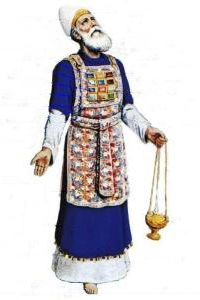
\includegraphics[width=50mm,scale=1.5]{Melchisedec.jpg}
\vspace{0.4in}

% Create a title for the document and write it in bold font
\LARGE{\textbf{\date}}
\linebreak

\vspace{0.5in}


\begin{flushleft}
\LARGE{Psalms 1-25 (Volume I)\\}\vspace{0.25in}
\LARGE{Notes, Outlines, Comments}
\end{flushleft}

% write in large letters
%\large{Free webservices and apps}

% Skip some space
\vspace{0.6in}

%\large{Documentation}
% Skip some space

\bigskip

\normalsize{Xenia, Oh.\\}
\normalsize{created: \today}

% Skip some space
\vspace{1.3in}

\end{flushright}
% End the title page
\end{titlepage}

%\titlehttps://www.overleaf.com/project/60d732302fc633866943c9d2JE

\newpage 

\tableofcontents\hypertarget{TOC}{}
\listoffigures
\listoftables

\hyphenation{A-bim-e-lech bre-thren E-phra-im  Gib-e-o-nites Jer-u-sa-lem through-out Phil-i-stines The-o-phil-us Am-a-le-kites ven-geance Mesh-el-e-mi-ah onan-ism Phar-a-oh Py-thon thoughts grev-ous-ness Hach-a-liah adul-ter-er Shad-rach}

%\fcolorbox{black}{bone}{TEXT}
%%%%%%%%%%%%%%%%% EXTRA COLORS
%%%%%%%%%%%%%%%%% EXTRA COLORS
%%%%%%%%%%%%%%%%% EXTRA COLORS
\definecolor{champagne}{rgb}{0.97,0.91,0.81}
\definecolor{bone}{rgb}{0.89,0.85,0.79}

\definecolor{ForestGreen}{rgb}{0.00,0.29,0.098}
\definecolor{GIVING}{cmyk}{1,0.0,0.72,.1}

\definecolor{MLPE}{cmyk}{1,1,0,.45}
\definecolor{SOCCER}{cmyk}{.77, 0, .42, .49}
\definecolor{PAYBILL}{cmyk}{0,0.83,0.76,0.07}
\definecolor{SERMON}{cmyk}{.14,.9,0,.30} % aka seance \href{http://www.flatuicolorpicker.com/purple-cmyk-color-model/}{seance}
\definecolor{BIBLE}{cmyk}{0,.17,.74,.17}
\definecolor{WORKBLUE}{cmyk}{1, .5, 0, .6}
\definecolor{myOrange}{cmyk}{0, .4, .98, .03}
\definecolor{myTan}{cmyk}{0.0,.07,.17,.10}
\definecolor{myRed}{cmyk}{0,1,1,0}
\definecolor{myWhite}{cmyk}{0,0,0,0}
\definecolor{BLUESoD}{cmyk}{.97,.84,0,.04}
\definecolor{WHITE}{cmyk}{0,0,0,0}
\definecolor{OLDGOLD}{cmyk}{0.05,0.3,1.00,0}
\definecolor{CASTLETON}{cmyk}{1,0,0.31,0.66}
\definecolor{cadmiumgreen}{rgb}{0.0, 0.42, 0.24}
\definecolor{jungle}{rgb}{0.203,0.4882,0.1718}
\definecolor{MYGOLD}{rgb}{1,.84,0}

\definecolor{MYLIGHTGRAY}{rgb}{.85,.85,.85}

\definecolor{codegreen}{rgb}{0,0.6,0}
\definecolor{codegray}{rgb}{0.5,0.5,0.5}
\definecolor{codepurple}{rgb}{0.58,0,0.82}
\definecolor{backcolour}{rgb}{0.95,0.95,0.92}



\mdfdefinestyle{MyFrame}{%
    linecolor=blue,
    outerlinewidth=2pt,
    roundcorner=5pt,
    innertopmargin=\baselineskip,
    innerbottommargin=\baselineskip,
    innerrightmargin=10pt,
    innerleftmargin=10pt,
    backgroundcolor=gray!25!white}


\mdfdefinestyle{MyFrame2}{%
    linecolor=black,
    outerlinewidth=2pt,
    roundcorner=5pt,
    innertopmargin=\baselineskip,
    innerbottommargin=\baselineskip,
    innerrightmargin=10pt,
    innerleftmargin=10pt,
    backgroundcolor=yellow!25!white}



%\input{PFTTIS}
%\input{WFTTIS}
%\input{WFITV}

%
%\newpage
%\begin{figure}
%\begin{center}
%\includegraphics[scale=.7, angle=0]{05OT-Deuteronomy/References/AndrewSmithDeuteronomyTimeline.png}
%\caption[Deuteronomy Timeline by Andrew Smith]{Deuteronomy Timeline by Andrew %Smith}
%\label{fig:Deuteronomy Timeline by Andrew Smith}
%\end{center}
%\end{figure}

\newpage
\begin{figure}
\begin{center}
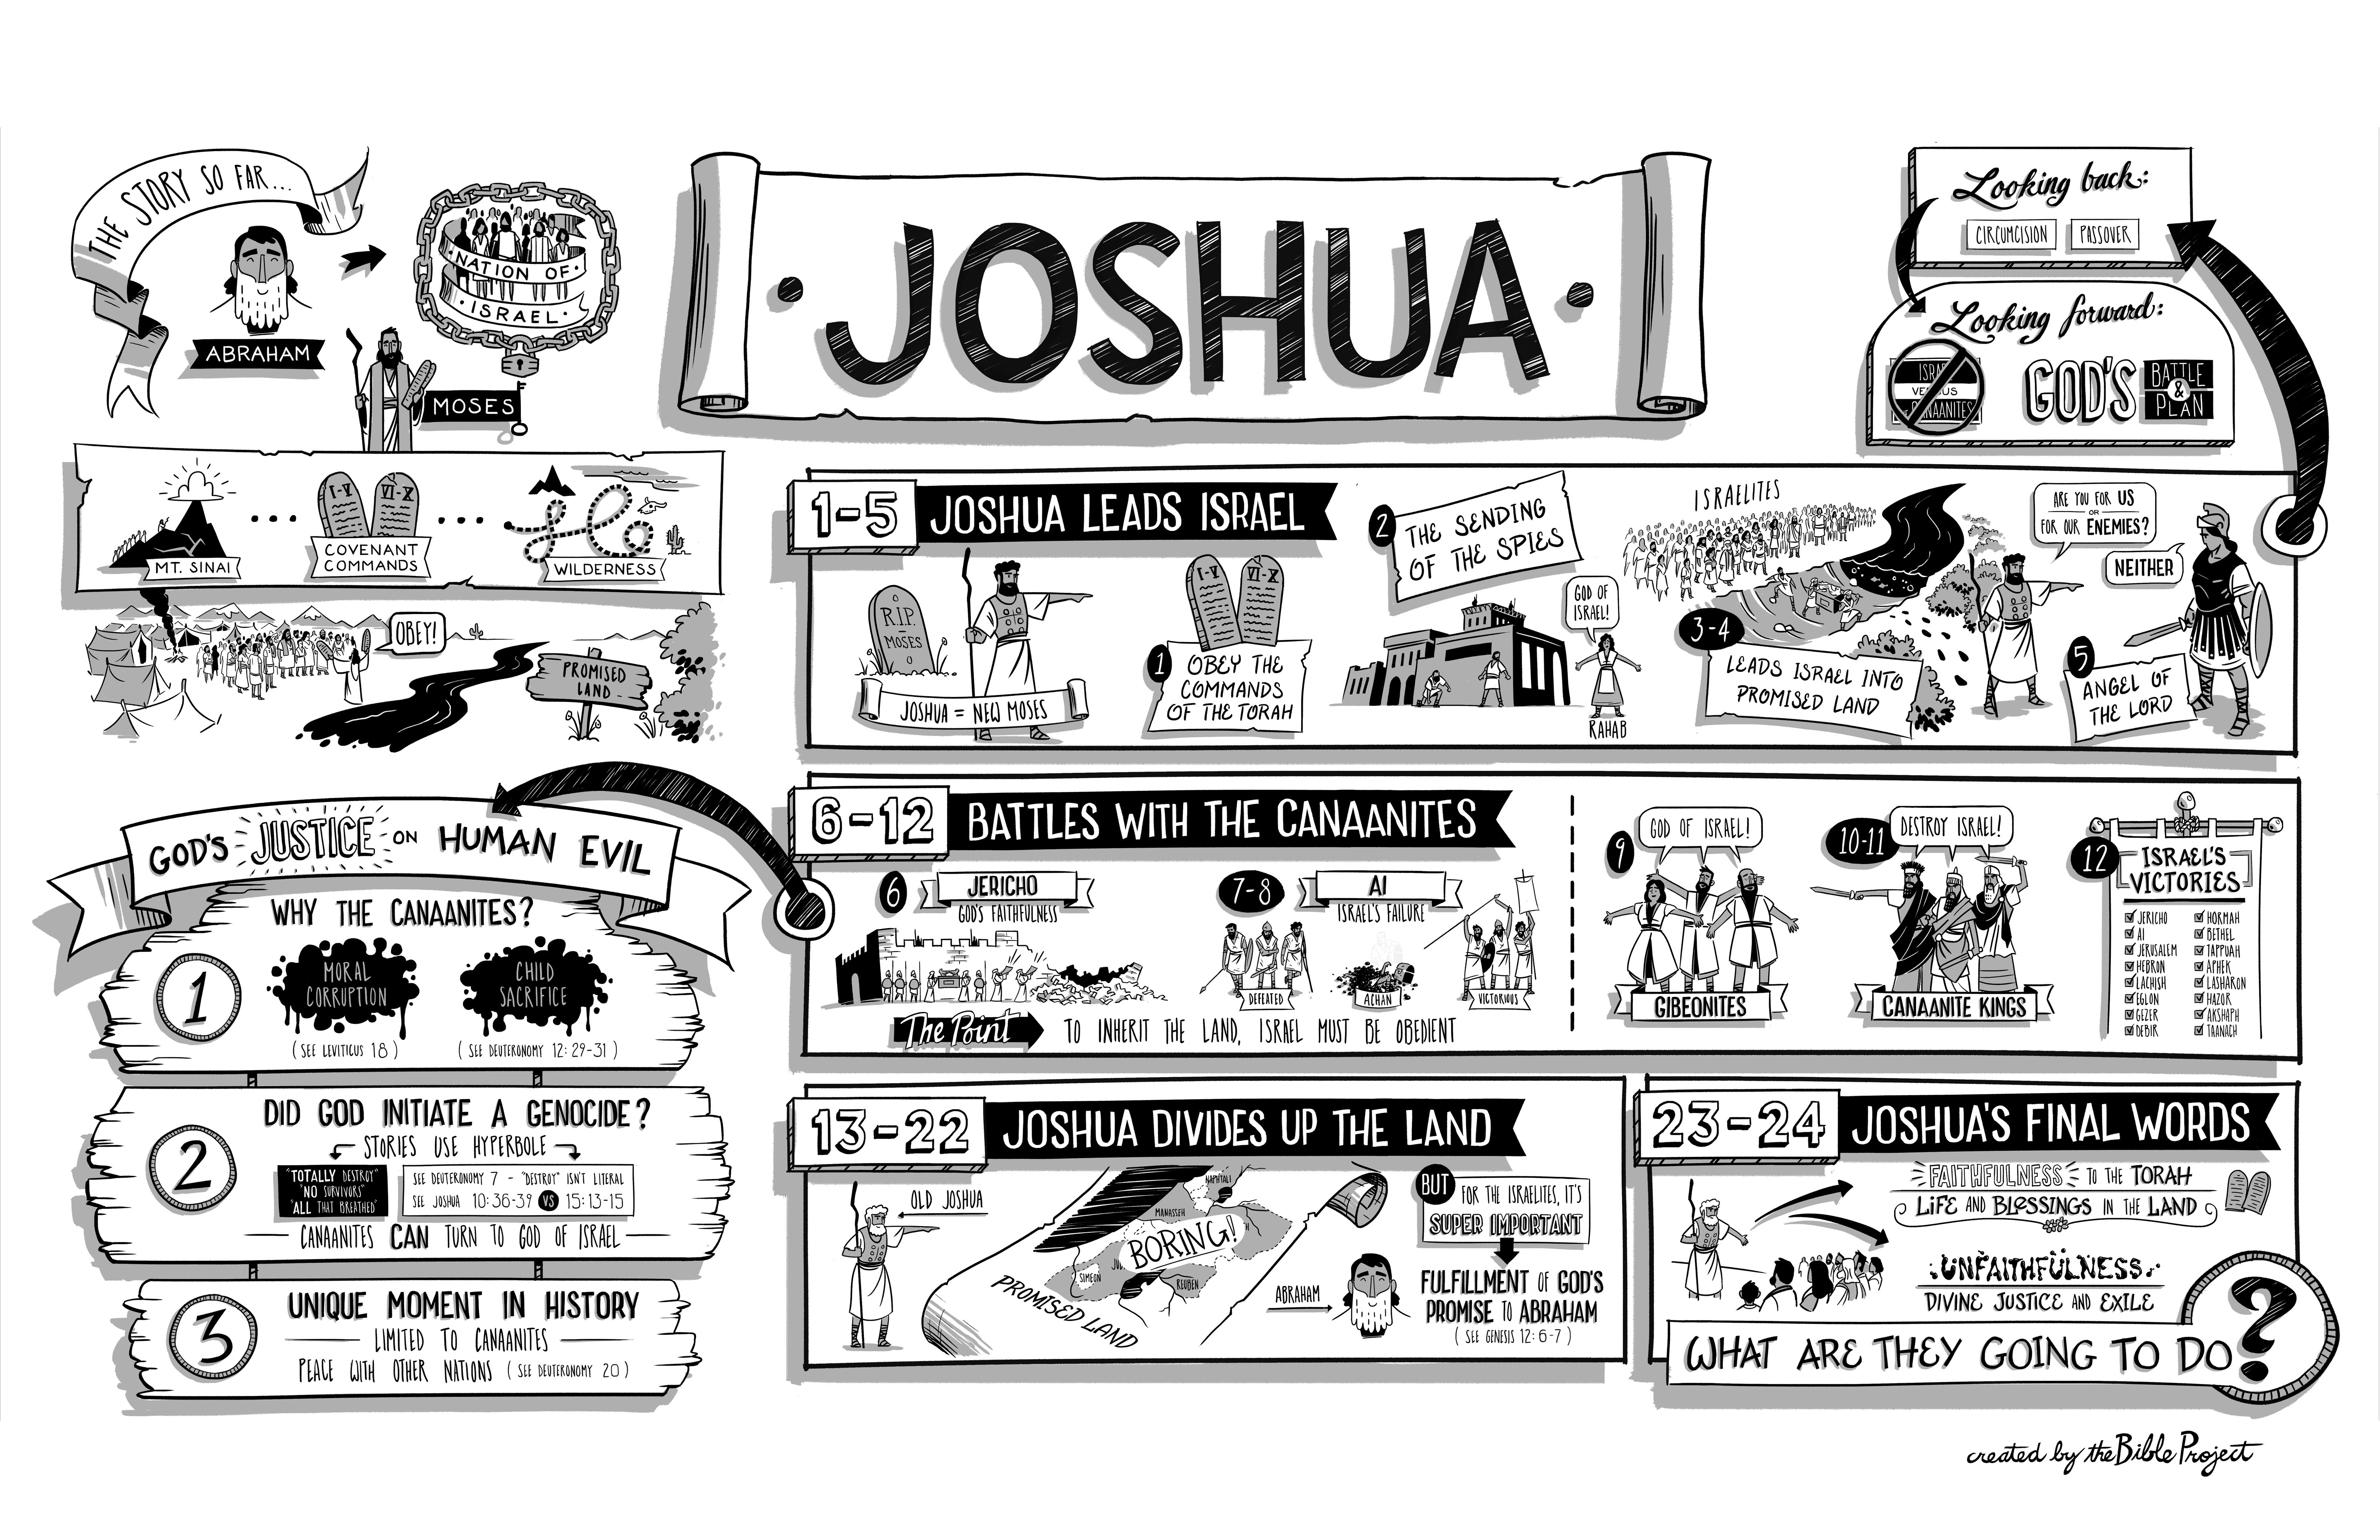
\includegraphics[scale=0.5, angle=90]{06OT-Joshua/References/1.BibleProject-Joshua.jpg}
\caption[Joshua from the Bible Project]{Joshua from the Bible Project}
\label{fig:Joshua from the Bible Project}
\end{center}
\end{figure}

\newpage
\begin{figure}
\begin{center}
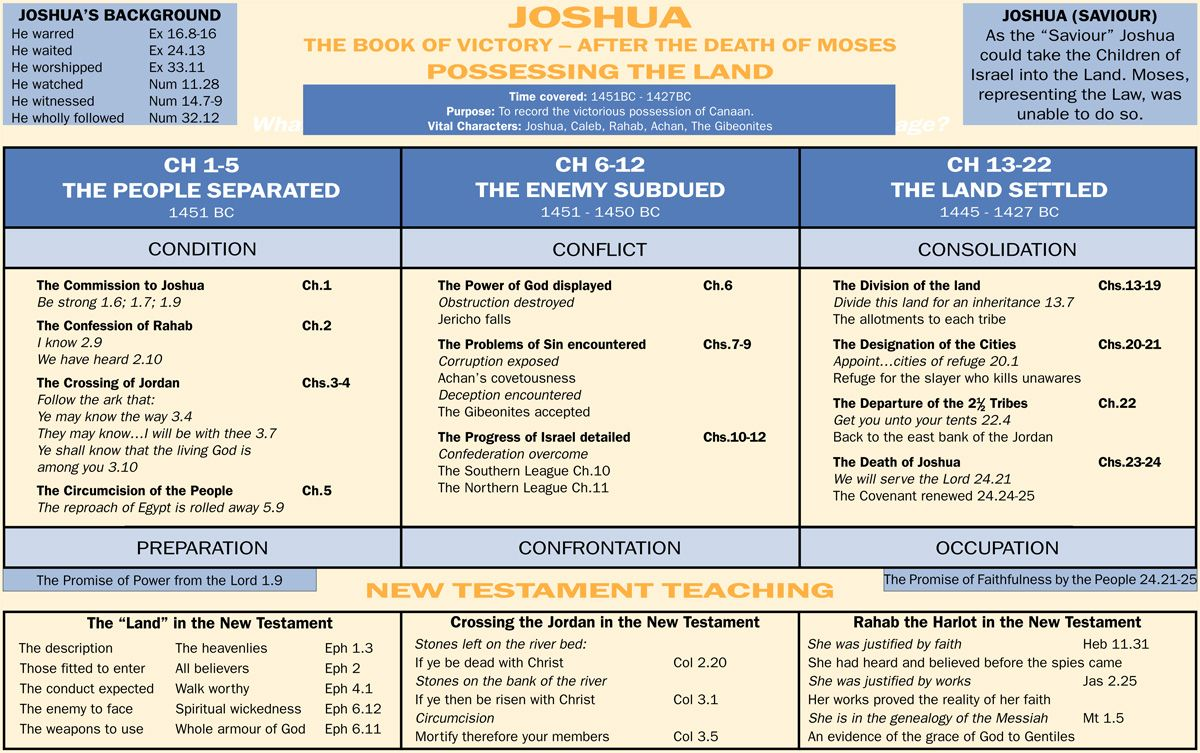
\includegraphics[scale=0.5, angle=90]{06OT-Joshua/References/2.JohnGrant-Joshua.jpg}
\caption[Joshua from John Grant]{Joshua from John Grant}
\label{fig:Joshua from John Grant}
\end{center}
\end{figure}

\newpage
\begin{figure}
\begin{center}
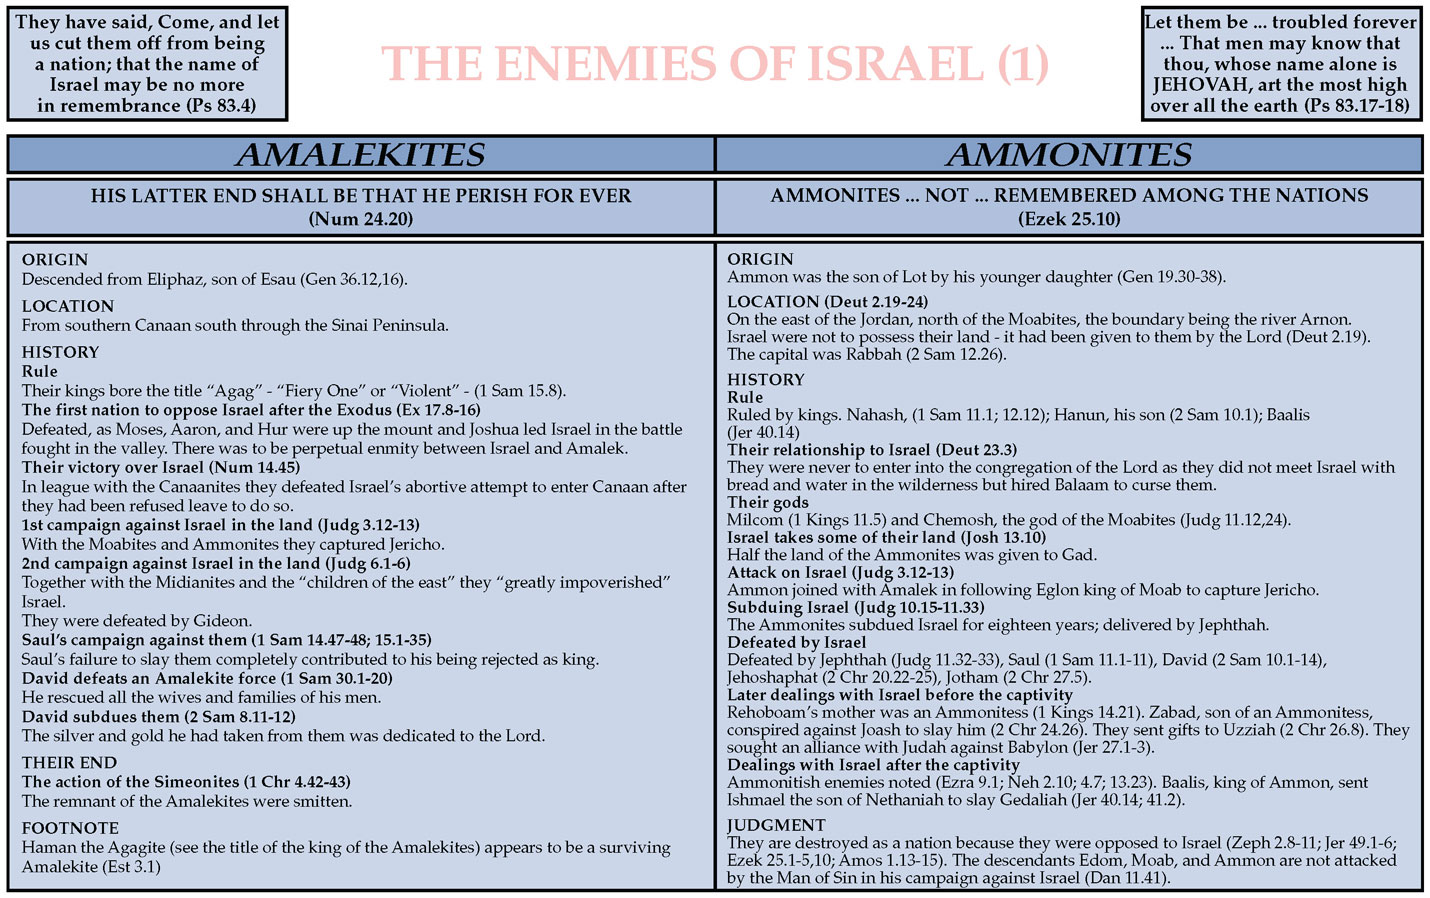
\includegraphics[scale=0.4, angle=90]{06OT-Joshua/References/3.EnemiesOfIsrael1.jpg}
\caption[Enemies of Israel 1]{Enemies of Israel 1}
\label{fig:Enemies of Israel 1}
\end{center}
\end{figure}

\newpage
\begin{figure}
\begin{center}
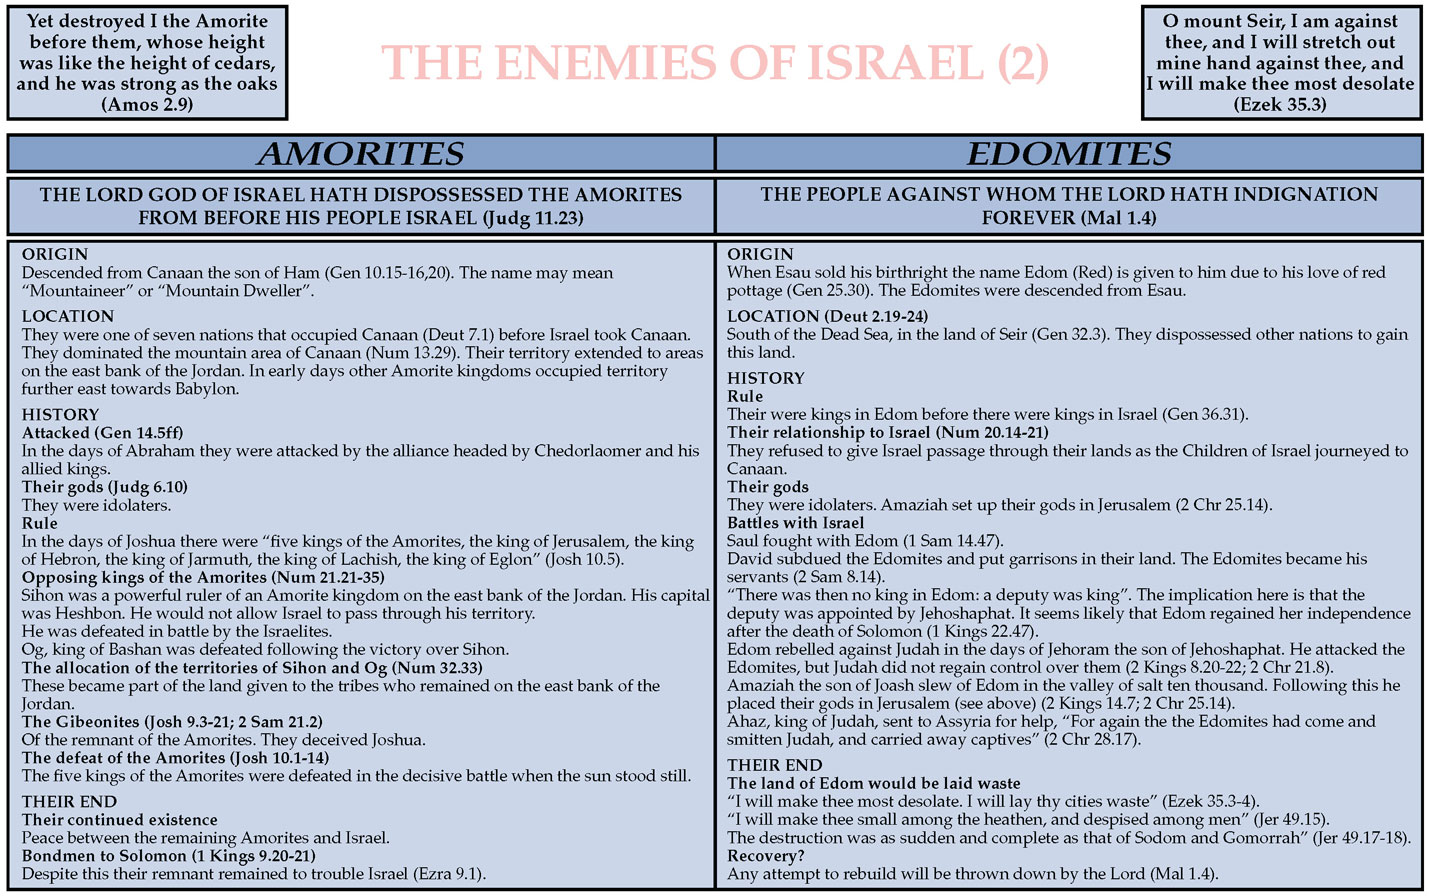
\includegraphics[scale=0.4, angle=90]{06OT-Joshua/References/4.EnemiesOfIsrael2.jpg}
\caption[Enemies of Israel 2]{Enemies of Israel 2}
\label{fig:Enemies of Israel 2}
\end{center}
\end{figure}

\newpage
\begin{figure}
\begin{center}
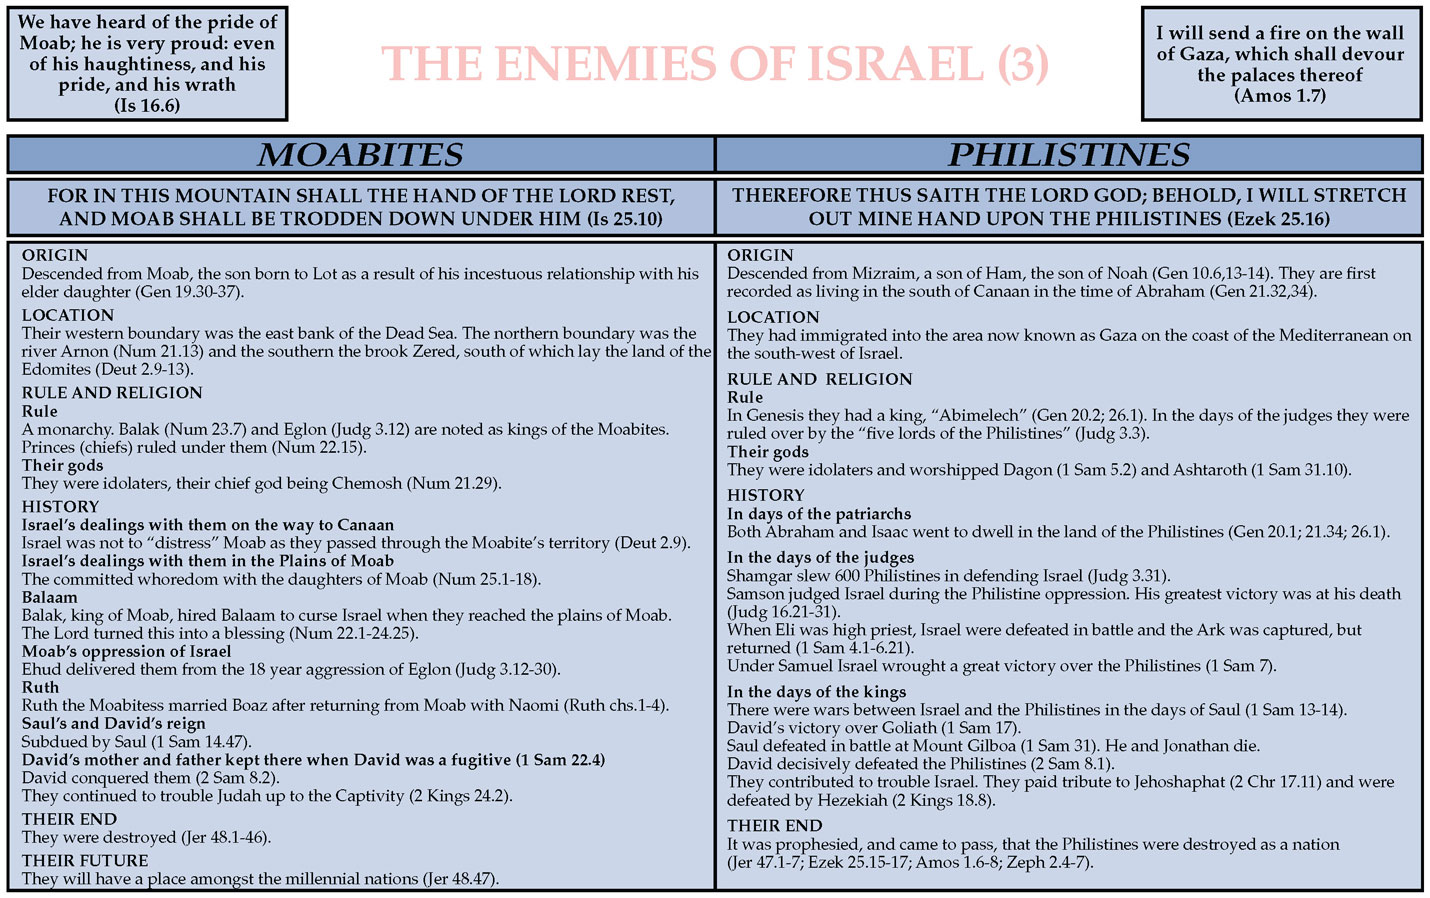
\includegraphics[scale=0.4, angle=90]{06OT-Joshua/References/5.EnemiesOfIsrael3.jpg}
\caption[Enemies of Israel 3]{Enemies of Israel 3}
\label{fig:Enemies of Israel 3}
\end{center}
\end{figure}

\newpage
\begin{figure}
\begin{center}
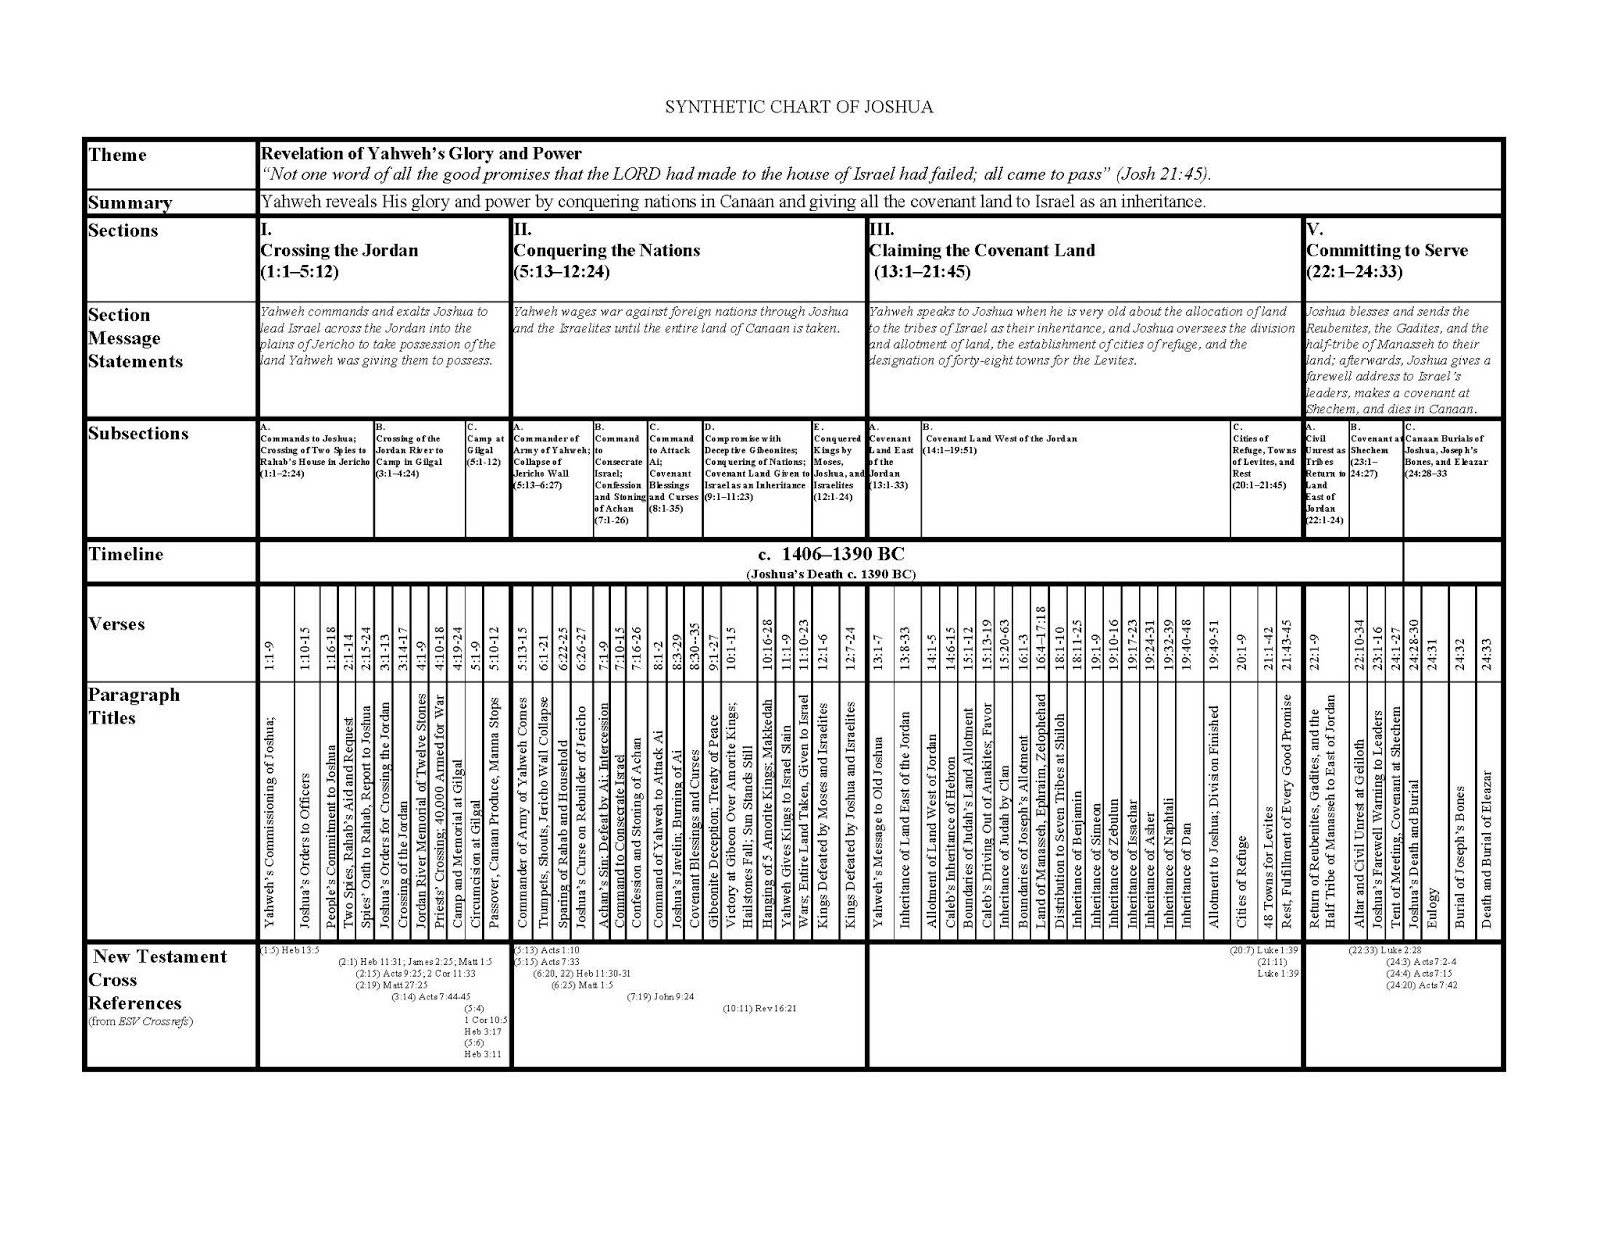
\includegraphics[scale=.4, angle=90]{06OT-Joshua/References/6.SyntheticChartofJoshua.jpg}
\caption[Synthetic Chart of Joshua]{Synthetic Chart of Joshua}
\label{fig:Synthetic Chart of Joshua}
\end{center}
\end{figure}


\newpage
\begin{figure}
\begin{center}
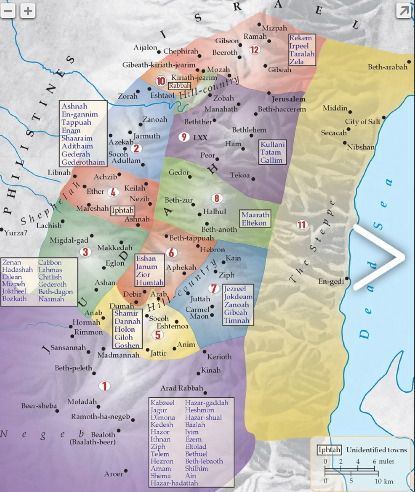
\includegraphics[scale=1, angle=0]{06OT-Joshua/References/7.WestSideOfDeadSea.jpg}
\caption[The West Side of the Dead Sea]{The West Side of the Dead Sea}
\label{fig:The West Side of the Dead Sea}
\end{center}
\end{figure}


\newpage
\begin{figure}
\begin{center}
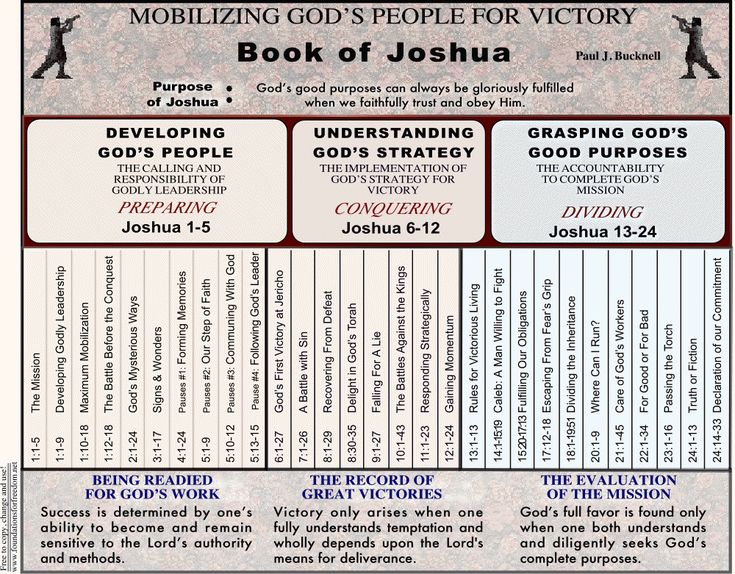
\includegraphics[scale=0.75, angle=90]{06OT-Joshua/References/8.Bucknell-Joshua.jpg}
\caption[Joshua from Bucknell]{Joshua from Bucknell}
\label{fig:Joshua from Bucknell}
\end{center}
\end{figure}


%\newpage
%\begin{figure}
%\begin{center}
%\includegraphics[scale=2, angle=90]{06OT-Joshua/References/9.Jensen-Joshua.png}
%\caption[Joshua from Jensen]{Joshua from Jensen}
%\label{fig:Joshua from Jensen}
%\end{center}
%\end{figure}


\newpage
\begin{figure}
\begin{center}
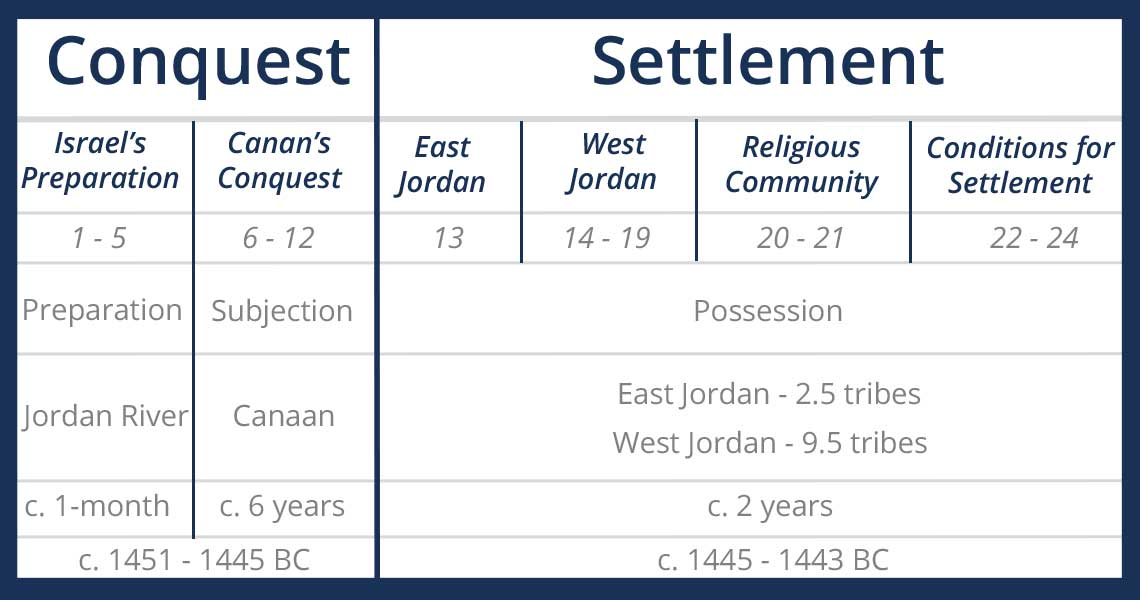
\includegraphics[scale=.5, angle=90]{06OT-Joshua/References/10.Bible-Brief-Joshua.jpg}
\caption[Bible Brief for Joshua]{Bible Brief for Joshua}
\label{fig:Bible Brief for Joshua}
\end{center}
\end{figure}

\newpage
\begin{figure}
\begin{center}
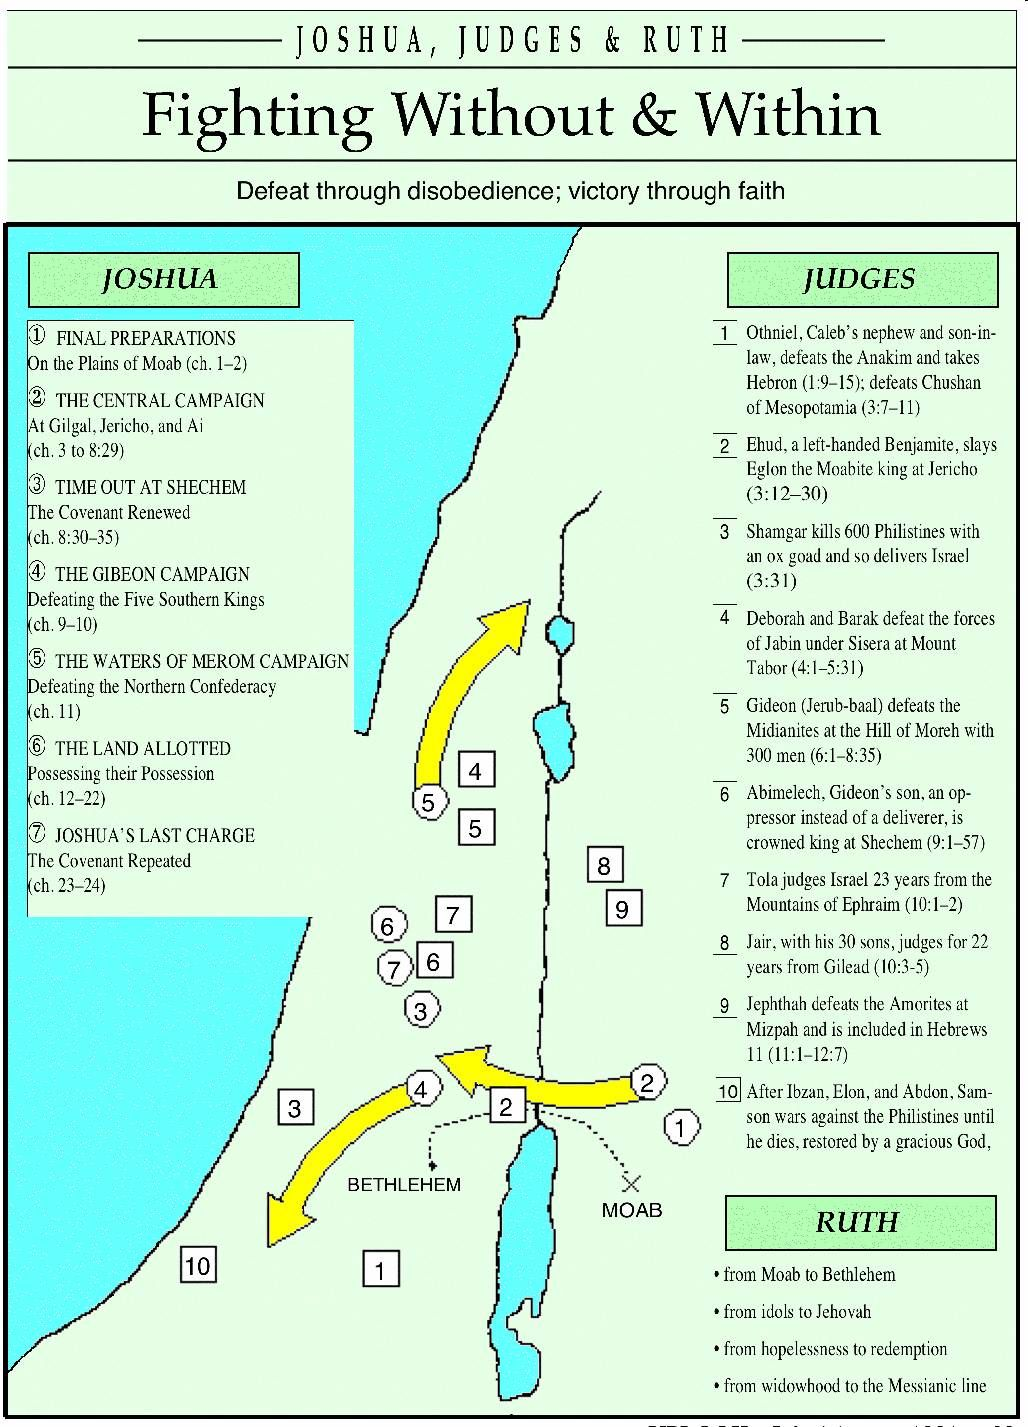
\includegraphics[scale=.5, angle=0]{06OT-Joshua/References/11.FightingInJoshuaAndJudges.jpg}
\caption[The Fighting in Joshua and Judges]{The Fighting in Joshua and Judges}
\label{fig:The Fighting in Joshua and Judges}
\end{center}
\end{figure}

\newpage
\begin{figure}
\begin{center}
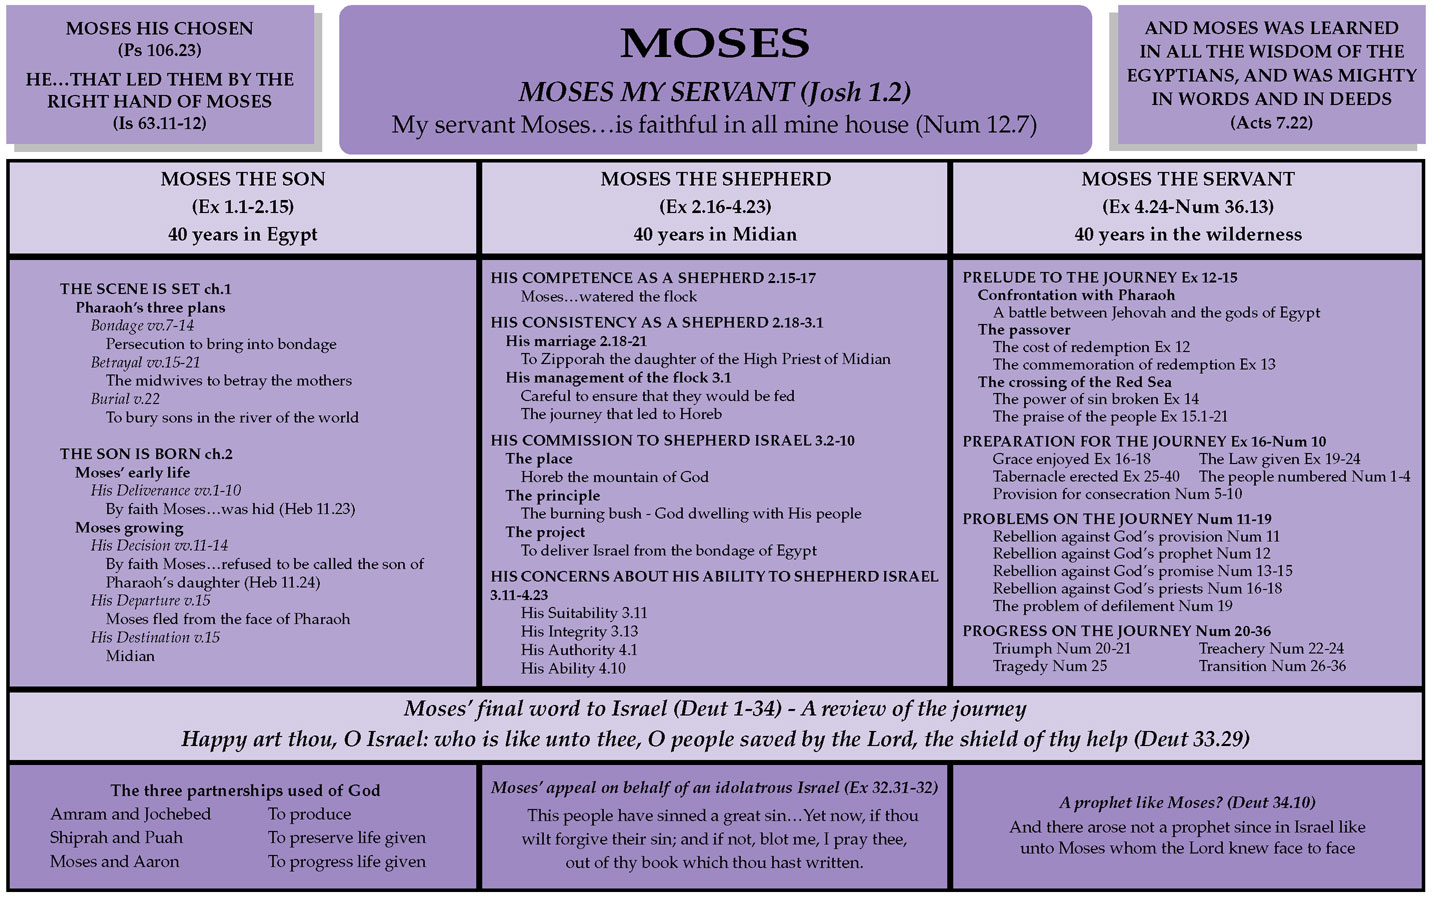
\includegraphics[scale=.4, angle=90]{06OT-Joshua/References/12.JohnGrantMoses.jpg}
\caption[Moses from John Grant]{Moses from John Grant}
\label{fig:Moses from John Grant}
\end{center}
\end{figure}







\chapter{Psalm 1}

\begin{figure}
  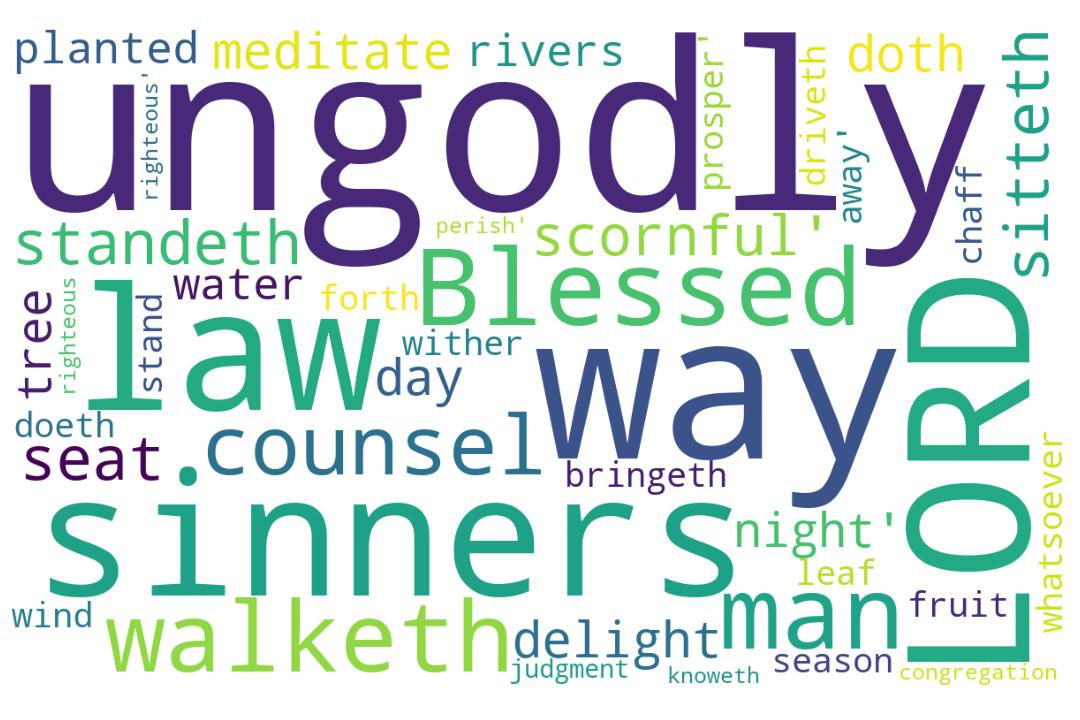
\includegraphics[width=\linewidth]{19OT-Psalms/Psalm1-WordCloud.jpg}
  \caption{Psalm 1 Word Cloud}
  \label{fig:Psalm 1 word Cloud}
\end{figure}


\marginpar{\scriptsize \centering \fcolorbox{bone}{lime}{\textbf{A PSALM OF COMPARISON}}\\ (Psalm 1) 
\begin{compactenum}[I.][8]
    \item A \textbf{Downward Cycle} \index[scripture]{Psalms!Psa 001:01}(Psa 1:1)
    \item A \textbf{Dialobical Counsel} \index[scripture]{Psalms!Psa 001:01}(Psa 1:1)
    \item \textbf{Diligent Consideration} \index[scripture]{Psalms!Psa 001:02}(Psa 1:2)
    \item A \textbf{Different Course} \index[scripture]{Psalms!Psa 001:02}(Psa 1:2)
    \item \textbf{Driven Chaff} \index[scripture]{Psalms!Psa 001:04}(Psa 1:4)
    \item \textbf{Distinguishing Characteristics}  \index[scripture]{Psalms!Psa 001:04}(Psa 1:4)
    \item A \textbf{Delivered Congregation} \index[scripture]{Psalms!Psa 001:05}(Psa 1:5)
    \item A \textbf{Definite Conclusion} \index[scripture]{Psalms!Psa 001:06}(Psa 1:6)
\end{compactenum} }

\marginpar{\scriptsize \centering \fcolorbox{bone}{yellow}{\textbf{THE PSALM 1 MAN}}\\ (Psalm 1) 
\begin{compactenum}[I.][8]
    \item \textbf{Shuns Fools} \index[scripture]{Psalms!Psa 001:01}(Psa 1:1)
    \item Has \textbf{Select Friends} \index[scripture]{Psalms!Psa 001:01}(Psa 1:1)
    \item Eats \textbf{Spiritual Food} \index[scripture]{Psalms!Psa 001:02}(Psa 1:2)
    \item Has \textbf{Special Fellowship} \index[scripture]{Psalms!Psa 001:02}(Psa 1:2)
    \item Exercises \textbf{Simple Faith} (All)
    \item Has his \textbf{Sins Forgiven} (All)
    \item He Can \textbf{Sense Falsehood}
    \item He \textbf{Sees the Future}
    \item Has a \textbf{Spectacular \& Secure Finish} \index[scripture]{Psalms!Psa 001:06}(Psa 1:6)
\end{compactenum}}



\marginpar{\scriptsize \centering \fcolorbox{bone}{black}{\textcolor{white}{\textbf{A COSMIC COMPARISON}}}\\ (Psalm 1) 
\begin{compactenum}[I.]
    \item They have Different \textbf{Objectives}
    \item They have Different \textbf{Orientations}
    \item They have Different \textbf{Obsessions}
    \item They have Different \textbf{Orientations}
    \item They have Different \textbf{Obstacles}
    \item They have Different \textbf{Outcomes}
\end{compactenum}}


\marginpar{\scriptsize \centering \fcolorbox{bone}{blue}{\textcolor{white}{\textbf{ON THE ROAD TO SCORN}}}\\ (Psalm 1) 
\begin{compactenum}[I.]
    \item Not \textbf{Recognizing Blessings}
    \item \textbf{Reviling the Brethren}
    \item Not \textbf{Reading the Book}
    \item \textbf{Revelling in Bitterness}
    \item Not \textbf{Remembering the Burdens}
    \item Not \textbf{Regarding the Body}
    \item Not Carrying the \textbf{Burdens of Believers}
\end{compactenum} }

\marginpar{\scriptsize \centering \fcolorbox{bone}{orange}{\textbf{THE UNGODLY}}\\ (Psalm 1) 

\begin{compactenum}[I.][8]
	\item ungodly \textbf{man} \index[scripture]{Psalms!Psa 001:01}  \index[scripture]{Psalms!Psa 001:04}  \index[scripture]{Psalms!Psa 001:05}  \index[scripture]{Psalms!Psa 003:07}  \index[scripture]{Psalms!Psa 018:04}  \index[scripture]{Proverbs!Pro 16:27} \index[scripture]{Romans!Rom 04:04} (Psa 1:1, 1:4, 1:5, 3:7, 18:4, Pro 16:27, Rom 4:4)
	\item ungoldy \textbf{men} \index[scripture]{2 Samuel!2Sam 22:05} \index[scripture]{2 Chronicles!2Chr 19:02} (2Sam 22:5, 2Chr 19:2, Job 16:11, Job 34:18, Psa 1:6, Psa 73:12, 1Tim 1:9, 1Pet 4:18, 2Pet 2:5, 2Pet 2:6, 2Pet 2:7, Jude 1:4, Jude 1:15)
	  \index[scripture]{Job!Job 16:11}\index[scripture]{Job!Job 34:18} \index[scripture]{Psalms!Psa 001:06} \index[scripture]{Psalms!Psa 073:12}\index[scripture]{1 Timothy!1Tim 01:09} \index[scripture]{1 Peter!1Pet 04:18}\index[scripture]{2 Peter!2Pet 02:05}\index[scripture]{2 Peter!2Pet 02:06}\index[scripture]{2 Peter!2Pet 02:07}\index[scripture]{Jude!Jude 01:15}
	\item ungodly \textbf{nation} \index[scripture]{Psalms!Psa 043:01} (Psa 43:1)
	\item ungodly \textbf{witness} \index[scripture]{Proverbs!Pro 19:28} (Pro 19:28)
	\item ungodly \textbf{deeds} \index[scripture]{Jude!Jude 01:15} (Jude 1:15)
	\item ungodly \textbf{actions} \index[scripture]{Jude!Jude 01:15} (Jude 1:15)
	\item ungodly \textbf{lusts} \index[scripture]{Jude!Jude 01:18} (Jude 1:18)
\end{compactenum}}



\footnote{\textcolor[cmyk]{0.99998,1,0,0}{\hyperlink{TOC}{Return to end of Table of Contents.}}}\footnote{\href{https://www.audioverse.org/english/audiobibles/books/ENGKJV/O/Ps/1}{\textcolor[cmyk]{0.99998,1,0,0}{Psalms Audio}}}\textcolor[cmyk]{0.99998,1,0,0}{Blessed is the man that \fcolorbox{bone}{lime}{walketh} not in the counsel of the \fcolorbox{bone}{lime}{ungodly}, nor \fcolorbox{bone}{lime}{standeth} in the way of sinners, nor \fcolorbox{bone}{lime}{sitteth} in the seat of the scornful.}
[2] \textcolor[cmyk]{0.99998,1,0,0}{But\textcolor{jungle}{$_{29}$} his delight is in the \fcolorbox{bone}{lime}{law of the LORD}; and in his law doth he meditate \fcolorbox{bone}{lime}{day and night}.}
[3] \textcolor[cmyk]{0.99998,1,0,0}{And\textcolor{jungle}{$_{49}$} he shall be like a tree planted by the rivers of water, that bringeth forth his fruit in his season; his leaf also shall not wither; and whatsoever he doeth shall prosper.}\footnote{\textbf{Jeremiah 17:8} -- For he shall be as a tree planted by the waters, and \emph{that} spreadeth out her roots by the river, and shall not see when heat cometh, but her leaf shall be green; and shall not be careful in the year of drought, neither shall cease from yielding fruit.}\footnote{The phrase ``rivers of water'' is found here in Psalm 1:3, Proverbs 21:1, Isaiah 32:2, and Lamentations 3:48. Interestingly, Isaiah 32:2 sets it in a Millennial context.}
[4] \textcolor[cmyk]{0.99998,1,0,0}{The\textcolor{jungle}{$_{82}$} ungodly are not so: but are \fcolorbox{bone}{lime}{like} the \fcolorbox{bone}{lime}{chaff} which the wind driveth away.}\footnote{The word ``chaff'' is found 14 times in 14 verses in scripture, only twice in the New Testament (Mathew 3:12 and Luke 3:17) speaking of the chaff which will be burnt up with unquenchable fire. See: (1) Job 21:18, (2)  Psalm 1:4 (here),  (3) Psalm 35:5, (4)  Isaiah 5:24, (5)  Isaiah 17:13, (6)  Isaiah 29:5, (7) Isaiah 33:11, (8)  Isaiah 41:15, (9) Jeremiah 23:28, (10) Daniel 2:35, (11) Hosea 13:3, (12) Zephaniah 2:2, (13) Matthew 3:12, and (14) Luke 3:17.} 
[5] \textcolor[cmyk]{0.99998,1,0,0}{Therefore\textcolor{jungle}{$_{113}$} the ungodly shall not stand in the judgment, nor sinners in the \fcolorbox{bone}{lime}{congregation} of the righteous.}
[6] \textcolor[cmyk]{0.99998,1,0,0}{For\textcolor{jungle}{$_{114}$} the LORD knoweth the way of the righteous: but the way of the ungodly \fcolorbox{bone}{lime}{shall perish}\textcolor{jungle}{$_{130}$}.}\footnote{\textbf{Psalm 49:12, 17--20} -- Nevertheless man being in honour abideth not: he is like the beasts that perish. [17]  For when he dieth he shall carry nothing away: his glory shall not descend after him.  [18]  Though while he lived he blessed his soul: and men will praise thee, when thou doest well to thyself. [19]  He shall go to the generation of his fathers; they shall never see light.  [20]  Man that is in honour, and understandeth not, is like the beasts that perish.}


\section{Psalm 1 Comments}

\subsection{Numeric Nuggets}
\textbf{13:} Verses 4 and 5 have 13 unique words.\\
\noindent \textbf{66:} There are 66 unique words in Psalm 1.

\subsection{Psalm 1 Introduction}
Note, there are (at least) seven distinct things spoken of in the psalm:
\begin{compactenum}
    \item The counsel of the ungodly [1]
    \item The way of sinners (equated with the way of the ungodly in verse 6) [1]
    \item The seat of the scornful [1]
    \item The Law of the LORD [2]
    \item A Tree planted by the rivers of water [3]
    \item The judgment [5]
    \item The congregation of the righteous [6]
\end{compactenum}


\subsection{Psalm 1:1}
Compare this to the opposite progression in Deuteronomy 5:1: Hear, learn, keep, and do.
%\index[NWIV]{28!Psalms!Psa 1:1}\index[AWIP]{Blessed!Psalms!Psa 1:1}\index[AWIP]{is!Psalms!Psa 1:1}\index[AWIP]{the!Psalms!Psa 1:1}\index[AWIP]{the!Psalms!Psa 1:1 (2)}\index[AWIP]{the!Psalms!Psa 1:1 (3)}\index[AWIP]{the!Psalms!Psa 1:1 (4)}\index[AWIP]{the!Psalms!Psa 1:1 (5)}\index[AWIP]{the!Psalms!Psa 1:1 (6)}\index[AWIP]{man!Psalms!Psa 1:1}\index[AWIP]{that!Psalms!Psa 1:1}\index[AWIP]{walketh!Psalms!Psa 1:1}\index[AWIP]{not!Psalms!Psa 1:1}\index[AWIP]{in!Psalms!Psa 1:1}\index[AWIP]{in!Psalms!Psa 1:1 (2)}\index[AWIP]{in!Psalms!Psa 1:1 (3)}\index[AWIP]{counsel!Psalms!Psa 1:1}\index[AWIP]{of!Psalms!Psa 1:1}\index[AWIP]{of!Psalms!Psa 1:1 (2)}\index[AWIP]{of!Psalms!Psa 1:1 (3)}\index[AWIP]{ungodly!Psalms!Psa 1:1}\index[AWIP]{nor!Psalms!Psa 1:1}\index[AWIP]{nor!Psalms!Psa 1:1 (2)}\index[AWIP]{standeth!Psalms!Psa 1:1}\index[AWIP]{way!Psalms!Psa 1:1}\index[AWIP]{sinners!Psalms!Psa 1:1}\index[AWIP]{sitteth!Psalms!Psa 1:1}\index[AWIP]{seat!Psalms!Psa 1:1}\index[AWIP]{scornful!Psalms!Psa 1:1}

\index[NWIV]{20!Psalms!Psa 1:2}\index[AWIP]{But!Psalms!Psa 1:2}\index[AWIP]{his!Psalms!Psa 1:2}\index[AWIP]{his!Psalms!Psa 1:2 (2)}\index[AWIP]{delight!Psalms!Psa 1:2}\index[AWIP]{is!Psalms!Psa 1:2}\index[AWIP]{in!Psalms!Psa 1:2}\index[AWIP]{in!Psalms!Psa 1:2 (2)}\index[AWIP]{the!Psalms!Psa 1:2}\index[AWIP]{the!Psalms!Psa 1:2 (2)}\index[AWIP]{law!Psalms!Psa 1:2}\index[AWIP]{law!Psalms!Psa 1:2 (2)}\index[AWIP]{of!Psalms!Psa 1:2}\index[AWIP]{LORD!Psalms!Psa 1:2}\index[AWIP]{and!Psalms!Psa 1:2}\index[AWIP]{and!Psalms!Psa 1:2 (2)}\index[AWIP]{doth!Psalms!Psa 1:2}\index[AWIP]{he!Psalms!Psa 1:2}\index[AWIP]{meditate!Psalms!Psa 1:2}\index[AWIP]{day!Psalms!Psa 1:2}\index[AWIP]{night!Psalms!Psa 1:2}

\index[NWIV]{33!Psalms!Psa 1:3}\index[AWIP]{And!Psalms!Psa 1:3}\index[AWIP]{he!Psalms!Psa 1:3}\index[AWIP]{he!Psalms!Psa 1:3 (2)}\index[AWIP]{shall!Psalms!Psa 1:3}\index[AWIP]{shall!Psalms!Psa 1:3 (2)}\index[AWIP]{shall!Psalms!Psa 1:3 (3)}\index[AWIP]{be!Psalms!Psa 1:3}\index[AWIP]{like!Psalms!Psa 1:3}\index[AWIP]{a!Psalms!Psa 1:3}\index[AWIP]{tree!Psalms!Psa 1:3}\index[AWIP]{planted!Psalms!Psa 1:3}\index[AWIP]{by!Psalms!Psa 1:3}\index[AWIP]{the!Psalms!Psa 1:3}\index[AWIP]{rivers!Psalms!Psa 1:3}\index[AWIP]{of!Psalms!Psa 1:3}\index[AWIP]{water!Psalms!Psa 1:3}\index[AWIP]{that!Psalms!Psa 1:3}\index[AWIP]{bringeth!Psalms!Psa 1:3}\index[AWIP]{forth!Psalms!Psa 1:3}\index[AWIP]{his!Psalms!Psa 1:3}\index[AWIP]{his!Psalms!Psa 1:3 (2)}\index[AWIP]{his!Psalms!Psa 1:3 (3)}\index[AWIP]{fruit!Psalms!Psa 1:3}\index[AWIP]{in!Psalms!Psa 1:3}\index[AWIP]{season!Psalms!Psa 1:3}\index[AWIP]{leaf!Psalms!Psa 1:3}\index[AWIP]{also!Psalms!Psa 1:3}\index[AWIP]{not!Psalms!Psa 1:3}\index[AWIP]{wither!Psalms!Psa 1:3}\index[AWIP]{and!Psalms!Psa 1:3}\index[AWIP]{whatsoever!Psalms!Psa 1:3}\index[AWIP]{doeth!Psalms!Psa 1:3}\index[AWIP]{prosper!Psalms!Psa 1:3}

\index[NWIV]{15!Psalms!Psa 1:4}\index[AWIP]{The!Psalms!Psa 1:4}\index[AWIP]{ungodly!Psalms!Psa 1:4}\index[AWIP]{are!Psalms!Psa 1:4}\index[AWIP]{are!Psalms!Psa 1:4 (2)}\index[AWIP]{not!Psalms!Psa 1:4}\index[AWIP]{so!Psalms!Psa 1:4}\index[AWIP]{but!Psalms!Psa 1:4}\index[AWIP]{like!Psalms!Psa 1:4}\index[AWIP]{the!Psalms!Psa 1:4}\index[AWIP]{the!Psalms!Psa 1:4 (2)}\index[AWIP]{chaff!Psalms!Psa 1:4}\index[AWIP]{which!Psalms!Psa 1:4}\index[AWIP]{wind!Psalms!Psa 1:4}\index[AWIP]{driveth!Psalms!Psa 1:4}\index[AWIP]{away!Psalms!Psa 1:4}

\index[NWIV]{17!Psalms!Psa 1:5}\index[AWIP]{Therefore!Psalms!Psa 1:5}\index[AWIP]{the!Psalms!Psa 1:5}\index[AWIP]{the!Psalms!Psa 1:5 (2)}\index[AWIP]{the!Psalms!Psa 1:5 (3)}\index[AWIP]{the!Psalms!Psa 1:5 (4)}\index[AWIP]{ungodly!Psalms!Psa 1:5}\index[AWIP]{shall!Psalms!Psa 1:5}\index[AWIP]{not!Psalms!Psa 1:5}\index[AWIP]{stand!Psalms!Psa 1:5}\index[AWIP]{in!Psalms!Psa 1:5}\index[AWIP]{in!Psalms!Psa 1:5 (2)}\index[AWIP]{judgment!Psalms!Psa 1:5}\index[AWIP]{nor!Psalms!Psa 1:5}\index[AWIP]{sinners!Psalms!Psa 1:5}\index[AWIP]{congregation!Psalms!Psa 1:5}\index[AWIP]{of!Psalms!Psa 1:5}\index[AWIP]{righteous!Psalms!Psa 1:5}

\index[NWIV]{17!Psalms!Psa 1:6}\index[AWIP]{For!Psalms!Psa 1:6}\index[AWIP]{the!Psalms!Psa 1:6}\index[AWIP]{the!Psalms!Psa 1:6 (2)}\index[AWIP]{the!Psalms!Psa 1:6 (3)}\index[AWIP]{the!Psalms!Psa 1:6 (4)}\index[AWIP]{the!Psalms!Psa 1:6 (5)}\index[AWIP]{LORD!Psalms!Psa 1:6}\index[AWIP]{knoweth!Psalms!Psa 1:6}\index[AWIP]{way!Psalms!Psa 1:6}\index[AWIP]{way!Psalms!Psa 1:6 (2)}\index[AWIP]{of!Psalms!Psa 1:6}\index[AWIP]{of!Psalms!Psa 1:6 (2)}\index[AWIP]{righteous!Psalms!Psa 1:6}\index[AWIP]{but!Psalms!Psa 1:6}\index[AWIP]{ungodly!Psalms!Psa 1:6}\index[AWIP]{shall!Psalms!Psa 1:6}\index[AWIP]{perish!Psalms!Psa 1:6}


\section{Psalm 1 Outlines}

\subsection{My Outlines}

\subsubsection{A Psalm of Comparisons}
\textbf{Introduction: }Psalm 1 compares the path of the righteous and the paths of the ungodly:
\index[speaker]{Keith Anthony!Psalm 001 (A Psalm of Comparisons)}
\index[series]{Psalms (Keith Anthony)!Psalm 001 (A Psalm of Comparisons)}
\index[date]{2015/08/24!Psalm 001 (A Psalm of Comparisons) (Keith Anthony)}
\begin{compactenum}[I.]
    \item A \textbf{Downward Cycle} \index[scripture]{Psalms!Psa 001:01}(Psa 1:1)
    \item A \textbf{Dialobical Counsel} \index[scripture]{Psalms!Psa 001:01}(Psa 1:1)
    \item \textbf{Diligent Consideration} \index[scripture]{Psalms!Psa 001:02}(Psa 1:2)
    \item A \textbf{Different Course} \index[scripture]{Psalms!Psa 001:02}(Psa 1:2)
    \item \textbf{Driven Chaff} \index[scripture]{Psalms!Psa 001:04}(Psa 1:4)
    \item \textbf{Distinguishing Characteristics}  \index[scripture]{Psalms!Psa 001:04}(Psa 1:4)
    \item A \textbf{Delivered Congregation} \index[scripture]{Psalms!Psa 001:05}(Psa 1:5)
    \item A \textbf{Definite Conclusion} \index[scripture]{Psalms!Psa 001:06}(Psa 1:6)
\end{compactenum}

\subsubsection{The Psalm 1 Man}
Psalm 1 provides a description of a different sort of man.  The man seeks God.  He seeks truth and righteousness.  He is radically different from the man of the world, and the man of the flesh, and the man who seeks the Devil. The Psalm 1 man: %\footnote{05 June 2015, Prepared for Lebanon Baptist Temple preaching class}
\index[speaker]{Keith Anthony!Psalm 001 (The Psalm 1 Man)}
\index[series]{Psalms (Keith Anthony)!Psalm 001 (The Psalm 1 Man)}
\index[date]{2015/06/05!Psalm 001 (The Psalm 1 Man) (Keith Anthony)}


\index[LOCATION]{Greene County Adult Detention Center!2022/01/11!Tuesday Night}

\begin{compactenum}[I.]
    \item \fcolorbox{bone}{yellow}{\textbf{Shuns Fools}} \index[scripture]{Psalms!Psa 001:01}(Psa 1:1) The word fool is used 66 times in the King James. The word ``fools'' is found another 42 times. ``Foolish'' is found 52 times! Foolishly, 12 times; foolishness, 20 times. That's 199 times that variants of the word are found (78 times in Proverbs).How about:
    \begin{compactenum}[A.]
		\item Psalm 14:1: The fool hath said in his heart, There is no God. They are corrupt, they have done abominable works, there is none that doeth good.
		\item Psalm 74:18:O LORD, and that the foolish people have blasphemed thy name.
		\item Proverb 27:3:  Though thou shouldest bray a fool in a mortar among wheat with a pestle, yet will not his foolishness depart from him. (stuck on folly)
	\end{compactenum}
    \item \fcolorbox{bone}{yellow}{Has \textbf{Select Friends}} \index[scripture]{Psalms!Psa 001:01}(Psa 1:1)
    \begin{compactenum}[A.]
    	\item 1 Corinthians 15:33 Be not deceived: evil communications corrupt good manners.
    	\item Proverb 12;26 The righteous is more excellent than his neighbour: but the way of the wicked seduceth them.
    	\item Proverb 13:20 He that walketh with wise men shall be wise: but a companion of fools shall be destroyed.
    	\item Proverb 20:19 He that goeth about as a talebearer revealeth secrets: therefore meddle not with him that flattereth with his lips.
    	\item Proverb 22:24-25 Make no friendship with an angry man; and with a furious man thou shalt not go: 25 Lest thou learn his ways, and get a snare to thy soul.
    	\item Proverb 24:6 For by wise counsel thou shalt make thy war: and in multitude of counsellors there is safety.
    	\item 2 Corinthians 6:14 Be ye not unequally yoked together with unbelievers: for what fellowship hath righteousness with unrighteousness? and what communion hath light with darkness?
    \end{compactenum}
	\item \fcolorbox{bone}{yellow}{Eats \textbf{Spiritual Food}} \index[scripture]{Psalms!Psa 001:02}(Psa 1:2) - Spiritual food is the blessings of God. It is typified by manna in the Old testament. Obedience is spiritual food. Doctrine is spiritual food. Worship is spiritual food. Prayer is spiritual food. Some verses:
    \begin{compactenum}[A.]
		\item 1 Corinthians 10:1-4 Moreover, brethren, I would not that ye should be ignorant, how that all our fathers were under the cloud, and all passed through the sea; 2 And were all baptized unto Moses in the cloud and in the sea; 3 And did all eat the same spiritual meat; 4 And did all drink the same spiritual drink: for they drank of that spiritual Rock that followed them: and that Rock was Christ.
		\item 1 Peter 2:2 As newborn babes, desire the sincere milk of the word, that ye may grow thereby:
		\item Hebrews 5:12-14 For when for the time ye ought to be teachers, ye have need that one teach you again which be the first principles of the oracles of God; and are become such as have need of milk, and not of strong meat. 13 For every one that useth milk is unskilful in the word of righteousness: for he is a babe. 14 But strong meat belongeth to them that are of full age, even those who by reason of use have their senses exercised to discern both good and evil.
		\item Jeremiah 3:15 And I will give you pastors according to mine heart, which shall feed you with knowledge and understanding.
		\item John 6:51 I am the living bread which came down from heaven: if any man eat of this bread, he shall live for ever: and the bread that I will give is my flesh, which I will give for the life of the world.
		\item Revealtion 2:7 He that hath an ear, let him hear what the Spirit saith unto the churches; To him that overcometh will I give to eat of the tree of life, which is in the midst of the paradise of God.
    \end{compactenum}
    \item \fcolorbox{bone}{yellow}{Has \textbf{Special Fellowship}} \index[scripture]{Psalms!Psa 001:02}(Psa 1:2) with God and with believers and with scripture
    \begin{compactenum}[A.]
    	\item Colossians 3:16 Let the word of Christ dwell in you richly in all wisdom; teaching and admonishing one another in psalms and hymns and spiritual songs, singing with grace in your hearts to the Lord.
		\item Romans 1:12 That is, that I may be comforted together with you by the mutual faith both of you and me.
		\item Hebrews 10:24-25 And let us consider one another to provoke unto love and to good works: 25 Not forsaking the assembling of ourselves together, as the manner of some is; but exhorting one another: and so much the more, as ye see the day approaching.
    \end{compactenum}
    \item \fcolorbox{bone}{yellow}{He Can \textbf{Sense Falsehood(s)} }
        \begin{compactenum}[A.]
        	\item 1 Chronicles 12:32 And of the children of Issachar, which were men that had understanding of the times, to know what Israel ought to do; the heads of them were two hundred; and all their brethren were at their commandment.
        	\item Psalm 119:105 Thy word is a lamp unto my feet, and a light unto my path.
        	\item Hebrews 5:15 But strong meat belongeth to them that are of full age, even those who by reason of use have their senses exercised to discern both good and evil.
           \end{compactenum}
     \item \fcolorbox{bone}{yellow}{He \textbf{Sees the Future}} Bible, carefully studied and rightly divided, records the essential human history and clearly lays out the future
    \begin{compactenum}[A.]
    	\item Amos 3:7 Surely the Lord GOD will do nothing, but he revealeth his secret unto his servants the prophets.
    	\item Acts 1:7-8 And he said unto them, It is not for you to know the times or the seasons, which the Father hath put in his own power. 8 But ye shall receive power, after that the Holy Ghost is come upon you: and ye shall be witnesses unto me both in Jerusalem, and in all Judæa, and in Samaria, and unto the uttermost part of the earth.
    \end{compactenum}
    \item \fcolorbox{bone}{yellow}{Has his \textbf{Sins Forgiven}} (All)
    \begin{compactenum}[A.]
    	\item Isaiah 1:18  Come now, and let us reason together, saith the LORD: though your sins be as scarlet, they shall be as white as snow; though they be red like crimson, they shall be as wool.
    	\item Isaiah 55:7  Let the wicked forsake his way, and the unrighteous man his thoughts: and let him return unto the LORD, and he will have mercy upon him; and to our God, for he will abundantly pardon.
    	\item John 3:1-17 For God so loved the world, that he gave his only begotten Son, that whosoever believeth in him should not perish, but have everlasting life. 17 For God sent not his Son into the world to condemn the world; but that the world through him might be saved.
    	\item Romans 6:23 For the wages of sin is death; but the gift of God is eternal life through Jesus Christ our Lord.
    	\item Romans 8:1 There is therefore now no condemnation to them which are in Christ Jesus, who walk not after the flesh, but after the Spirit.
		\item 1 John 1:9 If we confess our sins, he is faithful and just to forgive us our sins, and to cleanse us from all unrighteousness.
		\item 1 John 2:12 I write unto you, little children, because your sins are forgiven you for his name’s sake.
    \end{compactenum}
    \item \fcolorbox{bone}{yellow}{Has a \textbf{Spectacular \& Secure Finish}} \index[scripture]{Psalms!Psa 001:06}(Psa 1:6)
    \begin{compactenum}[A.]
		\item John 3:14-16 And as Moses lifted up the serpent in the wilderness, even so must the Son of man be lifted up: 15 That whosoever believeth in him should not perish, but have eternal life.
16 ¶ For God so loved the world, that he gave his only begotten Son, that whosoever believeth in him should not perish, but have everlasting life.
		\item Romans 6:23 For the wages of sin is death; but the gift of God is eternal life through Jesus Christ our Lord.
		\item John 4:14  But whosoever drinketh of the water that I shall give him shall never thirst; but the water that I shall give him shall be in him a well of water springing up into everlasting life.
		\item 1 John 2:25 And this is the promise that he hath promised us, even eternal life.
		\item Titus 3:3-7 For we ourselves also were sometimes foolish, disobedient, deceived, serving divers lusts and pleasures, living in malice and envy, hateful, and hating one another. 4 But after that the kindness and love of God our Saviour toward man appeared, 5 Not by works of righteousness which we have done, but according to his mercy he saved us, by the washing of regeneration, and renewing of the Holy Ghost; 6 Which he shed on us abundantly through Jesus Christ our Saviour; 7 That being justified by his grace, we should be made heirs according to the hope of eternal life. 
    \end{compactenum}
    \item Exercises \textbf{Simple Faith} (All)
    \begin{compactenum}[A.]
		\item Matthew 18:3 And said, Verily I say unto you, Except ye be converted, and become as little children, ye shall not enter into the kingdom of heaven
		\item Luke 18:17 Verily I say unto you, Whosoever shall not receive the kingdom of God as a little child shall in no wise enter therein
		\item Hebrews 11:6 ut without faith it is impossible to please him: for he that cometh to God must believe that he is, and that he is a rewarder of them that diligently seek him.
		\item Romans 10:17  So then faith cometh by hearing, and hearing by the word of God.
		\item Romans 1:17  For therein is the righteousness of God revealed from faith to faith: as it is written, The just shall live by faith.
    \end{compactenum}
\end{compactenum}

\subsubsection{A Cosmic Comparison}
Psalm 1 contrasts an ungodly man with one who seeks God Almighty. There are numerous differences.  Among them: %\footnote{04 June 2015, Prepared for Lebanon Baptist Temple preaching class}
\index[speaker]{Keith Anthony!Psalm 001 (A Cosmic Comparison)}
\index[series]{Psalms (Keith Anthony)!Psalm 001 (A Cosmic Comparison)}
\index[date]{2015/06/04!Psalm 001 (A Cosmic Comparison) (Keith Anthony)}
\begin{compactenum}[I.]
    \item They have Different \textbf{Objectives}
    \item They have Different \textbf{Orientations}
    \item They have Different \textbf{Obsessions}
    \item They have Different \textbf{Orientations}
    \item They have Different \textbf{Obstacles}
    \item They have Different \textbf{Outcomes}
\end{compactenum}

\subsubsection{Road-markers on the Road to Scorn}
I know a little bit about this, as does any Christian who has lived for more than a few years. Psalm 1 talks about the seat of the scornful.  Almost any Christian or every Christian has been abused by other Christians, mistreated by ministers, misunderstood, etc. Almost every Christian has been at one time or another on the wrong side of an apparent double-standard. These  are all dangerous place to be, as the response or rather how one decides to respond will make a world of difference. If you can picture Christianity as a highway, then there is also another parallel road, probably with a slow lane and a high-speed lane. At any point a Christian can exit off the Christian highway and get on this other road, going the opposite direction. Sometimes it is tough to recognize that you've done so. In Psalm 1, the destinations of these two roads are made known.  The place of blessing and the seat of the scornful. So, I got to thinking more about this road to this seat of the scornful.  What does the path look like?  What are the road-markers? This is just case you are seeing some of these road-markers of late.  Maybe you are on this road to the seat of the scornful. Maybe there are a few road signs that will tell you that you are: 
%\footnote{16 June 2015, Prepared for Lebanon Baptist Temple preaching class}
\index[speaker]{Keith Anthony!Psalm 001 (Road-markers on the Road to Scorn)}
\index[series]{Psalms (Keith Anthony)!Psalm 001 (Road-markers on the Road to Scorn)}
\index[date]{2015/06/16!Psalm 001 (Road-markers on the Road to Scorn) (Keith Anthony)}
\begin{compactenum}[I.]
    \item Not \textbf{Recognizing Blessings}
    \item \textbf{Reviling the Brethren}
    \item Not \textbf{Reading the Book}
    \item \textbf{Revelling in Bitterness}
    \item Not \textbf{Remembering the Burdens}
    \item Not \textbf{Regarding the Body}
    \item Not Carrying the \textbf{Burdens of Believers}
\end{compactenum}

\subsubsection{The Ungodly Man}
Psalm 1 provides insight into the ungodly man. The word ``ungodly'' is found 27 times in 24 verses in scripture, notably 4 times in Jude 15. Here is used in the corporate sense, as in ungodly people. Usages of the word: %\footnote{07 June 2016, Keith Anthony}
\index[speaker]{Keith Anthony!Psalm 001 (The Ungodly Man}
\index[series]{Psalms (Keith Anthony)!Psalm 001 (The Ungodly Man}
\index[date]{2016/06/07!Psalm 001 (The Ungodly Man (Keith Anthony)}
\begin{compactenum}[I.][8]
	\item ungodly \textbf{man} \index[scripture]{Psalms!Psa 001:01}  \index[scripture]{Psalms!Psa 001:04}  \index[scripture]{Psalms!Psa 001:05}  \index[scripture]{Psalms!Psa 003:07}  \index[scripture]{Psalms!Psa 018:04}  \index[scripture]{Proverbs!Pro 16:27} \index[scripture]{Romans!Rom 04:04} (Psa 1:1, 1:4, 1:5, 3:7, 18:4, Pro 16:27, Rom 4:4)
	\item ungoldy \textbf{men} \index[scripture]{2 Samuel!2Sam 22:05} \index[scripture]{2 Chronicles!2Chr 19:02} (2Sam 22:5, 2Chr 19:2, Job 16:11, Job 34:18, Psa 1:6, Psa 73:12, 1Tim 1:9, 1Pet 4:18, 2Pet 2:5, 2Pet 2:6, 2Pet 2:7, Jude 1:4, Jude 1:15)
	  \index[scripture]{Job!Job 16:11}\index[scripture]{Job!Job 34:18} \index[scripture]{Psalms!Psa 001:06} \index[scripture]{Psalms!Psa 073:12}\index[scripture]{1 Timothy!1Tim 01:09} \index[scripture]{1 Peter!1Pet 04:18}\index[scripture]{2 Peter!2Pet 02:05}\index[scripture]{2 Peter!2Pet 02:06}\index[scripture]{2 Peter!2Pet 02:07}\index[scripture]{Jude!Jude 01:15}
	\item ungodly \textbf{nation} \index[scripture]{Psalms!Psa 043:01} (Psa 43:1)
	\item ungodly \textbf{witness} \index[scripture]{Proverbs!Pro 19:28} (Pro 19:28)
	\item ungodly \textbf{deeds} \index[scripture]{Jude!Jude 01:15} (Jude 1:15)
	\item ungodly \textbf{actions} \index[scripture]{Jude!Jude 01:15} (Jude 1:15)
	\item ungodly \textbf{lusts} \index[scripture]{Jude!Jude 01:18} (Jude 1:18)
\end{compactenum}


\subsection{Outlines from Others}

\subsubsection{Bible Study as Worship}
Psalm 1 provides insight into the ungodly man. The word ``ungodly'' is found 27 times in 24 verses in scripture, notably 4 times in Jude 15. Here is used in the corporate sense, as in ungodly people. Usages of the word:\footnote{Kevin Cauley}\\ \\
\index[speaker]{Kevin Cauley!Psalm 001 (Bible Study as Worship}
\index[series]{Psalms (Kevin Cauley)!Psalm 001 (Bible Study as Worship}
\index[date]{2002/07/03!Psalm 001 (Bible Study as Worship) (Kevin Cauley)}
\noindent \textbf{Introduction: }A study of worship in the Bible. In this lesson we will look at Bible Study as Worship. Bible Study is worshiping God because we are 1) Reciting God's Will. 2) Respecting and Honoring God's Word. 3) Retaining God's thoughts in our hearts. 4) Retooling our lives in God's image.  Psalm 1:
\begin{compactenum}[1.][9]
	\item This first Psalm is a Psalm of introduction.
	\item It introduces us to the concept of studying God's word with the intention of applying it to life.
	\item A blessing is pronounced upon the one who does not progress in sin.
	\item He doesn't progress in sin because he has a delight in God's word.
	\item He meditates and thinks about God's word day and night.
	\item The beautiful results are that he is like a tree planted by the waters that brings forth fruit.
	\item This Psalm gives us a picture of worshiping God through the study of His word.
	\item Remember our definition of worship, to bend the knee and prostate oneself toward.
	\item How is this the case with Bible study?
\end{compactenum}
\textbf{\\Discussion: }Discussion: Christians worship God when we study His word because we are
\begin{compactenum}[I.][8]
	\item \textbf{Reciting God's Will} 
	\item  \textbf{Respecting and Honoring God's Words} 
	\item  \textbf{Retaining God's Words in Our Heart} 
	\item  \textbf{Retooling Our Lives in God's Image} 
\end{compactenum}

\subsubsection{Characteristics of the Successful Believer}
Psalm 1 provides insight into the ungodly man. The word ``ungodly'' is found 27 times in 24 verses in scripture, notably 4 times in Jude 15. Here is used in the corporate sense, as in ungodly people. Usages of the word: \\ \\
\index[speaker]{sermonnotebook.org!Psalm 001:01-06 (Characteristics of the Successful Believer}
\index[series]{Psalms (sermonnotebook.org)!Psalm 001 (Characteristics of the Successful Believer}
\index[date]{unknown!Psalm 001 (Characteristics of the Successful Believer) (sermonnotebook.org)}
\noindent \textbf{Introduction: }There are many yardsticks by which men measure success. Among them are: wealth, power, position, prestige, etc. These are all indicators of worldly success. However, measuring your spiritual success and your success as a Christian is a little more difficult. Often, there is little tangible, visible evidence, which you can put your hands on to prove you are living a successful Christian life. Generally, success for the believer is more internal that external. What I mean by that is this, the small amount of external evidence we produce is the result of much internal activity in our hearts and lives. That is why it is difficult for God’s children, who live in a materialistic world, to gauge their success in their walk with God. Thankfully Psalm 1 exists. In this worthy doorkeeper to the psalms, we find insight into what makes a believer successful. Tonight, as the plumbline of God’s Word moves alongside you life, see for yourself just how you measure up to God’s standard for successful Christian living. As we move through this Psalm, allow me to share with you The Characteristics Of The Successful Believer.

\begin{compactenum}[I.][8]
	\item The \textbf{Path} of the Successful Believer \index[scripture]{Psalms!Psa 001:01}(Psalm 1:1)
	\begin{compactenum}[A.]
		\item The Successful believer is separated in his walk of life.
		\item The downward progress – Walk, Stand, Sit. (This is the path Lot took – Gen. 19. It eventually led to his total downfall!)
		\item The successful believer realizes that there is a vast difference between himself and the world he was saved out of, and he lives accordingly!
	\end{compactenum}
	\item The \textbf{Pleasure} of the Successful Believer \index[scripture]{Psalms!Psa 001:02}(Psalm 1:2)
	\item The \textbf{Prosperity} of the Successful Believer \index[scripture]{Psalms!Psa 001:03}(Psalm 1:3)
	\begin{compactenum}[A.]
		\item His \textbf{Position} – By the River! Always close to the life giving resources. (ILLUSTRATION. This was meaningful to Israel with her mostly arid conditions.) The tree planted by the river is never dry and wilted, but is green, lush and lovely. (ILLUSTRATION. The believer who lives close to God will never be dry and wilted either. He will be vibrant, lively and productive.) (ILLUSTRATION. Many never know the joy of drawing off Christ daily! As a result, they are spiritually wilted and dead looking.) The droughts of life and the dry seasons never seem to affect the believer who is planted near the river. He is connected to an unfailing source of life and strength.
		\item His \textbf{Prominence} – ILLUSTRATION. A tree. The life of the successful believerstands heads above all those around him. It is easily seen when a man draws from the Lord. (Ill. Men will know when you have been with Jesus – Acts. 4:13)
		\item His \textbf{Permanence} – Planted – Unlike some plants, which live for a season and die out, this tree, has sunk its root deep and has a hidden source of life. (ILLUSTRATION. The value of private prayer and Bible Study.) (ILLUSTRATION. Planted – literally "transplanted." A tree cannot transplant itself, neither can a man transplant himself into the Kingdom of God. It is wholly a work of God’s grace. And, He always plants us in good soil, near the water supply. However, after we are planted, it is our responsibility to draw from the resources, which God has provided.)
		\item His \textbf{Productivity} – "Brings forth fruit" – The successful believer is a blessing to all those around him, because his fruit is plentiful. (ILLUSTRATION. John 7:38) (ILLUSTRATION. Old apple tree in the cow pasture. Man, cows, birds and insects all benefited from the fruit off this old tree.) (ILLUSTRATION. You may never know just who is feeding off your life!)
		\item His \textbf{Predictability} – "In his season" This tree isn’t a freak. Just as there are seasons of fruit bearing, so there are times of rest and growth. As believers, we aren’t to worry over the fruit. That is the Father’s business! When everything else is as it should be, then the fruit will come in its season – John 15:1-5.
		\item His \textbf{Perpetuity} – "leaf shall not fade" – The successful believer is like an evergreen. He is always surrounded by the green of life. (ILLUSTRATION. The trees in the wintertime. The hardwoods and leafy trees are look dead, but the evergreens stand out as islands of life in a sea of deadness. They are unaffected by winter or weather, but they are always the same.) (ILLUSTRATION. our lives should be lives of consistency! We are called on to be a stable, faithful and dependable people – 1 Cor. 15:58) The successful believer is consistent. The curve balls of life are unable to knock him off course. (ILLUSTRATION. Thank the Lord for consistent people!) (ILLUSTRATION. Life lived by this river in unchanging.)
		\item His \textbf{Prosperity} –"Whatsoever he doeth, it shall prosper" – In other words, God will bless the successful believer. His personal life, his family life, his business life, his church life, his spiritual life will all be blessed of the Lord. That isn’t to say that there won’t be stormy seas, but the successful believer will be able to sail them with Jesus until they are calm once again!
	\end{compactenum}
\end{compactenum}


\subsubsection{How to Identify a Blessed Man}
\index[speaker]{Clark Herring!Psalm 001 (How to Identify a Blessed Man}
\index[series]{Psalms (Clark Herring)!Psalm 001 (How to Identify a Blessed Man}
\index[date]{2018/01/10!Psalm 001 (How to Identify a Blessed Man) (Clark Herring)}
\begin{compactenum}[I.][6]
	\item His Decision \index[scripture]{Psalms!Psa 001:01}(Psalm 1:1)
	\begin{compactenum}[A.]
		\item Sprint (walk)
		\item Stand
		\item Seat
	\end{compactenum}	
	\item His Delight \index[scripture]{Psalms!Psa 001:02}(Psalm 1:2)
	\begin{compactenum}[A.]
		\item Law (2a)
		\item Lord (2b)
		\item Length (2c)
	\end{compactenum}	
	\item His Duration \index[scripture]{Psalms!Psa 001:03}(Psalm 1:3)
	\begin{compactenum}[A.]
		\item Fruitful (3a)
		\item Faithful (3b)
		\item Fortune (3c)
	\end{compactenum}	
	\item His Discouragement \index[scripture]{Psalms!Psa 001:04}(Psalm 1:4)
	\begin{compactenum}[A.]
		\item Satan
		\item Self
		\item Scorners
		\item Saints (jealousy)
	\end{compactenum}	
	\item His Destination \index[scripture]{Psalms!Psa 001:05}(Psalm 1:5)
	\begin{compactenum}[A.]
		\item We have a Place
		\item We have a Position
		\item We have a Pardon
	\end{compactenum}	
	\item His Direction \index[scripture]{Psalms!Psa 001:06}(Psalm 1:6)
	\begin{compactenum}[A.]
		\item Christ (6a)
		\item Confidence (6b)
		\item Comparison (6c)
	\end{compactenum}	
\end{compactenum}

\subsubsection{The Blessed Man}
\index[speaker]{Brian Eades!Psalm 01 (The Blessed Man)}
\index[series]{Psalm (Brian Eades)!Psalm 01 (The Blessed Man)}
\index[date]{2018/11/01!Psalm 01 (The Blessed Man) (Brian Eades)}
\textbf{Source}: Facebook, ``Sermon Hints'' group\\
\textbf{Introduction}: The Bible refers to the word "bless" 463 times; the word "curse" (being the antonym) which is mentioned only 183 times. What does it mean to be blessed? There are people on Earth who are blessed yet have no money or even health. Look at Job...His story is one of tragedy, yet he was the most blessed man on the face of the Earth!\\
\\
BLESSINGS-"Blissfully contented, definely or supremely favored, fortunate, that which brings thankfulness and appreciation."\\
\\
1 Timothy 6:6-10 (KJV) But godliness with contentment is great gain. For we brought nothing into this world, and it is certain we can carry nothing out. And having food and raiment let us be therewith content. But they that will be rich fall into temptation and a snare, and into many foolish and hurtful lusts, which drown men in destruction and perdition. For the love of money is the root of all evil: which while some coveted after, they have erred from the faith, and pierced themselves through with many sorrows.
\begin{compactenum}[I.][7]
	\item The \textbf{INTRODUCTION}   (of the entire Psalms) "Blessed"
	\item The \textbf{INDIVIDUALITY}   "is THE man"
	\item The \textbf{INSTRUCTIONS} 
	\begin{compactenum}[A.]
		\item AVOIDS BAD ADVICE
Walking not in the counsel of the ungodly
(backing)
		\item AVOIDS BAD ACTIONS
Standing not in the way of sinners (behavior)
		\item AVOIDS BAD ATTITUDES
Not sitting in the seat of the scornful (berating)
	\end{compactenum}
\item The \textbf{INSPIRATION} 
	\begin{compactenum}[A.]
		\item READING THE SCRIPTURES (comforted)
		\item ROOTED IN THE STREAM (consistent)
		\item REPRODUCTIVE IN THE SOIL (converting)
		\item READY FOR A SUCCESSFUL LIFE
	\end{compactenum}
\end{compactenum}
%\section{Psalm 1 Statistics}

%%%%%%%%%%%%%%%%%%%%%%%%%%%
%%%%%Word Statistics
%%%%%%%%%%%%%%%%%%%%%%%%%%%


\normalsize



\subsection{Chapter Word Statistics}


%%%%%%%%%%
%%%%%%%%%%
 
\begin{center}
\begin{longtable}{l|c|c|c|c}
\caption[Stats for Psalm 1]{Stats for Psalm 1} \label{table:Stats for Psalm 1} \\ 
\hline \multicolumn{1}{|c|}{\textbf{Verse(s)}} & \multicolumn{1}{|c|}{\textbf{Count}} & \multicolumn{1}{|c|}{\textbf{Unique}} & \multicolumn{1}{|c|}{\textbf{Italics}} & \multicolumn{1}{|c|}{\textbf{Uniq Italic}}  \\ \hline 
\endfirsthead
 
\multicolumn{5}{c}
{{\bfseries \tablename\ \thetable{} -- continued from previous page}} \\  
\hline \multicolumn{1}{|c|}{\textbf{Verse(s)}} & \multicolumn{1}{|c|}{\textbf{Count}} & \multicolumn{1}{|c|}{\textbf{Unique}} & \multicolumn{1}{|c|}{\textbf{Italics}} & \multicolumn{1}{|c|}{\textbf{Uniq Italic}}  \\ \hline 
\endhead
 
\hline \multicolumn{5}{|r|}{{Continued if needed}} \\ \hline
\endfoot 
1 & 28 & 18 & 0 & 0\\ \hline
2 & 20 & 15 & 0 & 0\\ \hline
3 & 33 & 28 & 0 & 0\\ \hline
4 & 15 & 13 & 0 & 0\\ \hline
5 & 17 & 13 & 0 & 0\\ \hline
6 & 17 & 11 & 0 & 0\\ \hline
\hline \hline
Total & 130 & 66 & 0 & 0



\end{longtable}
\end{center}

%%%%%%%%%%
%%%%%%%%%%
 
\subsection{Words by Frequency}

\begin{center}
\begin{longtable}{l|r}
\caption[Word Frequencies in Psalm 1]{Word Frequencies in Psalm 1} \label{table:WordsIn-Psalm-1} \\ 
\hline \multicolumn{1}{|c|}{\textbf{Word}} & \multicolumn{1}{c|}{\textbf{Frequency}} \\ \hline 
\endfirsthead
 
\multicolumn{2}{c}
{{\bfseries \tablename\ \thetable{} -- continued from previous page}} \\ 
\hline \multicolumn{1}{|c|}{\textbf{Word}} & \multicolumn{1}{c|}{\textbf{Frequency}} \\ \hline 
\endhead
 
\hline \multicolumn{2}{|r|}{{Continued if needed}} \\ \hline
\endfoot
 
\hline \hline
\endlastfoot
the & 20 \\ \hline
in & 8 \\ \hline
of & 8 \\ \hline
his & 5 \\ \hline
shall & 5 \\ \hline
not & 4 \\ \hline
ungodly & 4 \\ \hline
nor & 3 \\ \hline
way & 3 \\ \hline
and & 3 \\ \hline
he & 3 \\ \hline
is & 2 \\ \hline
that & 2 \\ \hline
sinners & 2 \\ \hline
law & 2 \\ \hline
LORD & 2 \\ \hline
like & 2 \\ \hline
are & 2 \\ \hline
but & 2 \\ \hline
righteous & 2 \\ \hline
Blessed & 1 \\ \hline
man & 1 \\ \hline
walketh & 1 \\ \hline
counsel & 1 \\ \hline
standeth & 1 \\ \hline
sitteth & 1 \\ \hline
seat & 1 \\ \hline
scornful & 1 \\ \hline
But & 1 \\ \hline
delight & 1 \\ \hline
doth & 1 \\ \hline
meditate & 1 \\ \hline
day & 1 \\ \hline
night & 1 \\ \hline
And & 1 \\ \hline
be & 1 \\ \hline
a & 1 \\ \hline
tree & 1 \\ \hline
planted & 1 \\ \hline
by & 1 \\ \hline
rivers & 1 \\ \hline
water & 1 \\ \hline
bringeth & 1 \\ \hline
forth & 1 \\ \hline
fruit & 1 \\ \hline
season & 1 \\ \hline
leaf & 1 \\ \hline
also & 1 \\ \hline
wither & 1 \\ \hline
whatsoever & 1 \\ \hline
doeth & 1 \\ \hline
prosper & 1 \\ \hline
The & 1 \\ \hline
so & 1 \\ \hline
chaff & 1 \\ \hline
which & 1 \\ \hline
wind & 1 \\ \hline
driveth & 1 \\ \hline
away & 1 \\ \hline
Therefore & 1 \\ \hline
stand & 1 \\ \hline
judgment & 1 \\ \hline
congregation & 1 \\ \hline
For & 1 \\ \hline
knoweth & 1 \\ \hline
perish & 1 \\ \hline
\end{longtable}
\end{center}



\normalsize



\subsection{Words Alphabetically}

\begin{center}
\begin{longtable}{l|r}
\caption[Word Alphabetically in Psalm 1]{Word Alphabetically in Psalm 1} \label{table:WordsIn-Psalm-1} \\ 
\hline \multicolumn{1}{|c|}{\textbf{Word}} & \multicolumn{1}{c|}{\textbf{Frequency}} \\ \hline 
\endfirsthead
 
\multicolumn{2}{c}
{{\bfseries \tablename\ \thetable{} -- continued from previous page}} \\ 
\hline \multicolumn{1}{|c|}{\textbf{Word}} & \multicolumn{1}{c|}{\textbf{Frequency}} \\ \hline 
\endhead
 
\hline \multicolumn{2}{|r|}{{Continued if needed}} \\ \hline
\endfoot
 
\hline \hline
\endlastfoot
And & 1 \\ \hline
Blessed & 1 \\ \hline
But & 1 \\ \hline
For & 1 \\ \hline
LORD & 2 \\ \hline
The & 1 \\ \hline
Therefore & 1 \\ \hline
a & 1 \\ \hline
also & 1 \\ \hline
and & 3 \\ \hline
are & 2 \\ \hline
away & 1 \\ \hline
be & 1 \\ \hline
bringeth & 1 \\ \hline
but & 2 \\ \hline
by & 1 \\ \hline
chaff & 1 \\ \hline
congregation & 1 \\ \hline
counsel & 1 \\ \hline
day & 1 \\ \hline
delight & 1 \\ \hline
doeth & 1 \\ \hline
doth & 1 \\ \hline
driveth & 1 \\ \hline
forth & 1 \\ \hline
fruit & 1 \\ \hline
he & 3 \\ \hline
his & 5 \\ \hline
in & 8 \\ \hline
is & 2 \\ \hline
judgment & 1 \\ \hline
knoweth & 1 \\ \hline
law & 2 \\ \hline
leaf & 1 \\ \hline
like & 2 \\ \hline
man & 1 \\ \hline
meditate & 1 \\ \hline
night & 1 \\ \hline
nor & 3 \\ \hline
not & 4 \\ \hline
of & 8 \\ \hline
perish & 1 \\ \hline
planted & 1 \\ \hline
prosper & 1 \\ \hline
righteous & 2 \\ \hline
rivers & 1 \\ \hline
scornful & 1 \\ \hline
season & 1 \\ \hline
seat & 1 \\ \hline
shall & 5 \\ \hline
sinners & 2 \\ \hline
sitteth & 1 \\ \hline
so & 1 \\ \hline
stand & 1 \\ \hline
standeth & 1 \\ \hline
that & 2 \\ \hline
the & 20 \\ \hline
tree & 1 \\ \hline
ungodly & 4 \\ \hline
walketh & 1 \\ \hline
water & 1 \\ \hline
way & 3 \\ \hline
whatsoever & 1 \\ \hline
which & 1 \\ \hline
wind & 1 \\ \hline
wither & 1 \\ \hline
\end{longtable}
\end{center}



\normalsize



\subsection{Word Lengths in Chapter}
\normalsize
\begin{longtable}{l|p{3.75in}}
\caption[Words by Length in Psalm 1]{Words by Length in Psalm 1} \label{table:WordsIn-Psalm-1} \\ 
\hline \multicolumn{1}{|c|}{\textbf{Length}} & \multicolumn{1}{c|}{\textbf{Words}} \\ \hline 
\endfirsthead
 
\multicolumn{2}{c}
{{\bfseries \tablename\ \thetable{} -- continued from previous page}} \\ 
\hline \multicolumn{1}{|c|}{\textbf{Length}} & \multicolumn{1}{c|}{\textbf{Words}} \\ \hline 
\endhead
 
\hline \multicolumn{2}{|r|}{{Continued if needed}} \\ \hline
\endfoot
 
\hline \hline
\endlastfoot
1 & a \\ \hline
2 & is, in, of, he, be, by, so \\ \hline
3 & the, man, not, nor, way, But, his, law, and, day, And, The, are, but, For \\ \hline
4 & that, seat, LORD, doth, like, tree, leaf, also, wind, away \\ \hline
5 & night, shall, water, forth, fruit, doeth, chaff, which, stand \\ \hline
6 & rivers, season, wither, perish \\ \hline
7 & Blessed, walketh, counsel, ungodly, sinners, sitteth, delight, planted, prosper, driveth, knoweth \\ \hline
8 & standeth, scornful, meditate, bringeth, judgment \\ \hline
9 & Therefore, righteous \\ \hline
10 & whatsoever \\ \hline
12 & congregation \\ \hline
\end{longtable}






%%%%%%%%%%
%%%%%%%%%%
\subsection{Psalm1 Repeated Phrases}


%%%%%%%%%%
%%%%%%%%%%
\normalsize
 
\begin{center}
\begin{longtable}{|p{3.0in}|p{0.5in}|}
\caption[Psalm1 Repeated Phrases]{Psalm1 Repeated Phrases}\label{table:Repeated Phrases Psalm1} \\
\hline \multicolumn{1}{|c|}{\textbf{Phrase}} & \multicolumn{1}{c|}{\textbf{Frequency}} \\ \hline 
\endfirsthead
 
\multicolumn{2}{c}
{{\bfseries \tablename\ \thetable{} -- continued from previous page}} \\  
\hline \multicolumn{1}{|c|}{\textbf{Phrase}} & \multicolumn{1}{c|}{\textbf{Frequency}} \\ \hline 
\endhead
 
\hline \multicolumn{2}{c}{{ }} \\ \hline
\endfoot 
in the & 6\\ \hline 
of the & 6\\ \hline 
the ungodly & 3\\ \hline 
the way & 3\\ \hline 
the way of & 3\\ \hline 
way of & 3\\ \hline 
\end{longtable}
\end{center}



%%%%%%%%%%
%%%%%%%%%%




\chapter{Psalm 2}

\begin{figure}
  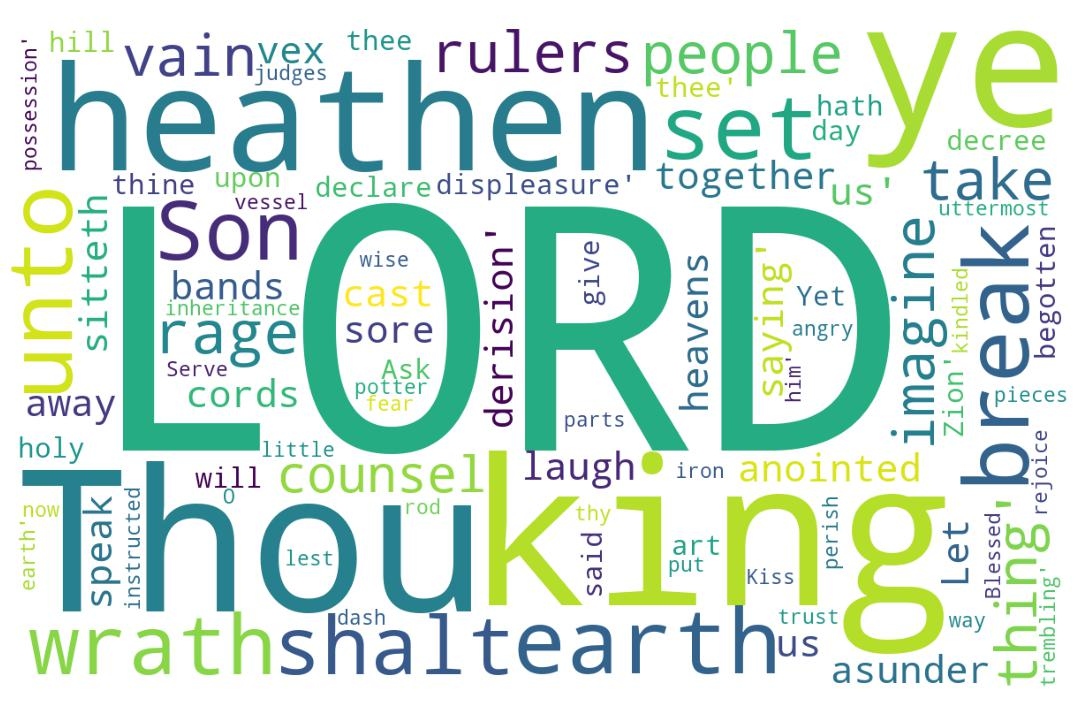
\includegraphics[width=\linewidth]{19OT-Psalms/Psalm2-WordCloud.jpg}
  \caption{Psalm 2 Word Cloud}
  \label{fig:Psalm 2 word Cloud}
\end{figure}


\marginpar{\scriptsize \centering \fcolorbox{bone}{lime}{\textbf{WHY THE HEATHEN RAGE (I)}}\\ (Psalm 2:1-12) 
\begin{compactenum}[I.][8]
    \item They have no \textbf{Savior}
    \item They have no \textbf{Seed}
    \item They have no \textbf{Seekers}
    \item They have no \textbf{Supplication}
    \item They have no \textbf{Security}
    \item They have no \textbf{Substance}
    \item They have no \textbf{Salvation}
\end{compactenum} }

\marginpar{\scriptsize \centering \fcolorbox{bone}{yellow}{\textbf{WHY THE HEATHEN RAGE (II)}}\\ (Psalm 2:1-12) 
\begin{compactenum}[I.][8]
    \item \textbf{Utter Rebellion} (Futility) \index[scripture]{Psalms!Psa 002:01-03} (Psa 2:1-3)
    \item \textbf{Undaunted Religion} (Ferocity) \index[scripture]{Psalms!Psa 002:04-06} (Psa 2:4-6)
    \item \textbf{Unrestrained Ridicule} \index[scripture]{Psalms!Psa 002:04} (Psa 2:4)
    \item \textbf{Ultimate Reign} (Finality) \index[scripture]{Psalms!Psa 002:07-09} (Psa 2:7-9)
    \item \textbf{Untimely Return} (Fire) \index[scripture]{Psalms!Psa 002:09} (Psa 2:9)
    \item \textbf{Unmitigated Ruin} (Finish) \index[scripture]{Psalms!Psa 002:09} (Psa 2:9)
    \item \textbf{Urgent Recommendation} (Fear) \index[scripture]{Psalms!Psa 002:10-12} (Psa 2:10-12)
    \item \textbf{Un-applied Repentance} (Forgiveness) \index[scripture]{Psalms!Psa 002:12} (Psa 2:12)
\end{compactenum} }

\marginpar{\scriptsize \centering \fcolorbox{bone}{black}{\textcolor{white}{\textbf{MAN, KNOWING HIS PLACE}}}\\ (Psalm 2:1-12) 
\begin{compactenum}[I.][8]
    \item The \textbf{Rage}  \index[scripture]{Psalms!Psa 002:01} (Psa 2:1)
    \item The \textbf{Rebellion}  \index[scripture]{Psalms!Psa 002:02} (Psa 2:2)
    \item The \textbf{Restraint}  \index[scripture]{Psalms!Psa 002:03} (Psa 2:3)
    \item The \textbf{Ruin}  \index[scripture]{Psalms!Psa 002:09} (Psa 2:9)
    \item The \textbf{Repentance}  \index[scripture]{Psalms!Psa 002:11} (Psa 2:11)
    \item The \textbf{Rejoicing}  \index[scripture]{Psalms!Psa 002:01} (Psa 2:1)
    \item The \textbf{Reality}  \index[scripture]{Psalms!Psa 002:12} (Psa 2:12)
\end{compactenum} }

\footnote{\textcolor[cmyk]{0.99998,1,0,0}{\hyperlink{TOC}{Return to end of Table of Contents.}}}\footnote{\href{https://www.audioverse.org/english/audiobibles/books/ENGKJV/O/Ps/1}{\textcolor[cmyk]{0.99998,1,0,0}{Psalms Audio}}}\textcolor[cmyk]{0.99998,1,0,0}{Why\textcolor{jungle}{$_{131}$} do the heathen rage, and the people imagine a vain thing?}
[2] \textcolor[cmyk]{0.99998,1,0,0}{The\textcolor{jungle}{$_{143}$} kings of the earth set themselves, and the rulers take \fcolorbox{bone}{yellow}{counsel} together, against the LORD, and against his anointed, \emph{saying},}
[3] \textcolor[cmyk]{0.99998,1,0,0}{Let\textcolor{jungle}{$_{164}$} us break their bands asunder, and cast away their cords from us.}
[4] \textcolor[cmyk]{0.99998,1,0,0}{He\textcolor{jungle}{$_{177}$} that sitteth in the heavens shall \fcolorbox{bone}{yellow}{laugh}: the Lord shall have them in \fcolorbox{bone}{yellow}{derision}.}
[5] \textcolor[cmyk]{0.99998,1,0,0}{Then\textcolor{jungle}{$_{192}$} shall he speak unto them in his \fcolorbox{bone}{yellow}{wrath}, and vex them in his sore displeasure.}
[6] \textcolor[cmyk]{0.99998,1,0,0}{Yet\textcolor{jungle}{$_{208}$} have I set my king upon my holy hill of Zion.}
[7] \textcolor[cmyk]{0.99998,1,0,0}{I\textcolor{jungle}{$_{220}$} will declare the decree: the LORD hath said unto me, Thou \emph{art} my Son; this day have I begotten thee.}
[8] \textcolor[cmyk]{0.99998,1,0,0}{Ask\textcolor{jungle}{$_{241}$} of me, and I shall give \emph{thee} the heathen \emph{for} \fcolorbox{bone}{yellow}{thine inheritance}, and the uttermost parts of the earth \emph{for} thy possession.}
[9] \textcolor[cmyk]{0.99998,1,0,0}{Thou\textcolor{jungle}{$_{264}$} shalt \fcolorbox{bone}{yellow}{break them} with a rod of iron; thou shalt \fcolorbox{bone}{yellow}{dash them} in pieces like a potter's vessel.}
[10] \textcolor[cmyk]{0.99998,1,0,0}{\fcolorbox{bone}{yellow}{Be}\textcolor{jungle}{$_{283}$} \fcolorbox{bone}{yellow}{wise} now therefore, O ye kings: be instructed, ye judges of the earth.}
[11] \textcolor[cmyk]{0.99998,1,0,0}{Serve\textcolor{jungle}{$_{297}$} the LORD with fear, and rejoice with trembling.}
[12] \textcolor[cmyk]{0.99998,1,0,0}{\fcolorbox{bone}{yellow}{Kiss\textcolor{jungle}{$_{306}$} the Son}, lest he be angry, and ye perish \emph{from} the way, when his wrath is kindled but a little. Blessed \emph{are} all they that put their trust in him\textcolor{jungle}{$_{336}$}.}


\section{Psalm 2 Comments}



\subsection{Psalm 2:1, 2}
Modern translations corrupt this verse.\footnote{\textbf{Isaiah 40:17} - All nations before him are as nothing; and they are counted to him less than nothing, and vanity.} But these heathen are everywhere.  The rage. They rule.  They rise up. They mostly reject. They ruin things.  Theses heathen are the ones to whome the gospel is to be preached in Galatians 1:16, 2:9, and 3:8.\footnote{\textbf{Galatians 1:16} - To reveal his Son in me, that I might preach him among the heathen; immediately I conferred not with flesh and blood:}\footnote{\textbf{Galatians 2:9} - And when James, Cephas, and John, who seemed to be pillars, perceived the grace that was given unto me, they gave to me and Barnabas the right hands of fellowship; that we should go unto the heathen, and they unto the circumcision.}\footnote{\textbf{Galatians 3:8} - And the scripture, foreseeing that God would justify the heathen through faith, preached before the gospel unto Abraham, saying, In thee shall all nations be blessed.}\\
\\
\noindent Verses 1 and 2 are used in Acts 4:27 to describe the collection of Pilate, Herod, the Gentiles, Christ-rejecting Israelites, organized religion, and organized politics, to rise up and destroy God's work on Earth.  But this rebellion was only partially fulfilled.\cite{Ruckman1992PsalmsV1} The future focus of united mankind (typified in Genesis 11) will be this rebellion.
%%%%%%%%%%%%%%%%%%%%%%%%%%%%%%%%%%%%%%%%%%%%%%%%%

%%%%%%%%%%%%%%%%%%%%%%%%%%%%%%%%%%%%%%%%%%%%%%%%

\begin{center}

\begin{table}[ht]
\centering
\begin{tabular}{|p{.5in}|p{3.5in}|}
\hline

\textcolor[rgb]{0.00,0.00,1.00}{AV} & \textcolor[rgb]{0.00,0.00,1.00}{Why do the heathen rage, and the people imagine a vain thing?} \\ 
\hline \hline

ASV &  Why do the nations rage, And the peoples meditate a vain thing? \\ \hline
%
CEB &  Why do the nations rant?   Why do the peoples rave uselessly?\\ \hline
%
ESV & Why do the nations rage and the peoples plot in vain? \\ \hline
%
NASV &  Why are the nations restless And the peoples plotting in vain? \\ \hline
%
MEV & Why do the nations rage,  and the peoples plot in vain?\\ \hline
%
NIV &  Why do the nations conspire  and the peoples plot in vain? \\ \hline
%
NKJV &  Why do the nations rage, And the people plot a vain thing? \\ \hline
%
RSV &  Why do the nations conspire, and the peoples plot in vain?\\ \hline \hline

\multicolumn{2}{|p{4.2in}|}{{\textcolor{jungle}{Modern translations soften and dilute the verse by changing the word `heathen'' to ``nations.'' It is almnost as if to say that only some of the ``nations'' are ``heathen.'' These nations are  identified in Isaiah 40:17.}}} \\ \hline

\end{tabular}
\caption[Corruption Alert: Psalm 2:1]{Corruption Alert: Psalm 2:1} \label{table:CorruptionPsalm-2-1}
\end{table}

\end{center}

%%%%%%%%%%%%%%%%%%%%%%%%%%%%%%%%%%%%%%%%%%%%%%%%





\subsection{Psalm 2:3}
There are some sort of ``bands'' and ``cords'' that are currently preventing the conclusion of this rage. Something like this is described in Isaiah 30:28 and Matthew 13:30. Something like this is described in 2 Thessalonians 2:6.\footnote{\textbf{Isaiah 30:28} - And his breath, as an overflowing stream, shall reach to the midst of the neck, to sift the nations with the sieve of vanity: and there shall be a bridle in the jaws of the people, causing them to err.}\footnote{\textbf{Matthew 13:30} - The field is the world; the good seed are the children of the kingdom; but the tares are the children of the wicked one;}\footnote{\textbf{2 Thessalonians 2:6} - And now ye know what withholdeth that he might be revealed in his time.} \cite{Ruckman1992PsalmsV1}

%\index[NWIV]{12!Psalms!Psa 2:1}\index[AWIP]{Why!Psalms!Psa 2:1}\index[AWIP]{do!Psalms!Psa 2:1}\index[AWIP]{the!Psalms!Psa 2:1}\index[AWIP]{the!Psalms!Psa 2:1 (2)}\index[AWIP]{heathen!Psalms!Psa 2:1}\index[AWIP]{rage!Psalms!Psa 2:1}\index[AWIP]{and!Psalms!Psa 2:1}\index[AWIP]{people!Psalms!Psa 2:1}\index[AWIP]{imagine!Psalms!Psa 2:1}\index[AWIP]{a!Psalms!Psa 2:1}\index[AWIP]{vain!Psalms!Psa 2:1}\index[AWIP]{thing?!Psalms!Psa 2:1}

\index[NWIV]{21!Psalms!Psa 2:2}\index[AWIP]{The!Psalms!Psa 2:2}\index[AWIP]{kings!Psalms!Psa 2:2}\index[AWIP]{of!Psalms!Psa 2:2}\index[AWIP]{the!Psalms!Psa 2:2}\index[AWIP]{the!Psalms!Psa 2:2 (2)}\index[AWIP]{the!Psalms!Psa 2:2 (3)}\index[AWIP]{earth!Psalms!Psa 2:2}\index[AWIP]{set!Psalms!Psa 2:2}\index[AWIP]{themselves!Psalms!Psa 2:2}\index[AWIP]{and!Psalms!Psa 2:2}\index[AWIP]{and!Psalms!Psa 2:2 (2)}\index[AWIP]{rulers!Psalms!Psa 2:2}\index[AWIP]{take!Psalms!Psa 2:2}\index[AWIP]{counsel!Psalms!Psa 2:2}\index[AWIP]{together!Psalms!Psa 2:2}\index[AWIP]{against!Psalms!Psa 2:2}\index[AWIP]{against!Psalms!Psa 2:2 (2)}\index[AWIP]{LORD!Psalms!Psa 2:2}\index[AWIP]{his!Psalms!Psa 2:2}\index[AWIP]{anointed!Psalms!Psa 2:2}\index[AWIP]{\emph{saying}!Psalms!Psa 2:2}\index[AWIP]{\emph{saying}!Psalms!Psa 2:2}

\index[NWIV]{13!Psalms!Psa 2:3}\index[AWIP]{Let!Psalms!Psa 2:3}\index[AWIP]{us!Psalms!Psa 2:3}\index[AWIP]{us!Psalms!Psa 2:3 (2)}\index[AWIP]{break!Psalms!Psa 2:3}\index[AWIP]{their!Psalms!Psa 2:3}\index[AWIP]{their!Psalms!Psa 2:3 (2)}\index[AWIP]{bands!Psalms!Psa 2:3}\index[AWIP]{asunder!Psalms!Psa 2:3}\index[AWIP]{and!Psalms!Psa 2:3}\index[AWIP]{cast!Psalms!Psa 2:3}\index[AWIP]{away!Psalms!Psa 2:3}\index[AWIP]{cords!Psalms!Psa 2:3}\index[AWIP]{from!Psalms!Psa 2:3}

\index[NWIV]{15!Psalms!Psa 2:4}\index[AWIP]{He!Psalms!Psa 2:4}\index[AWIP]{that!Psalms!Psa 2:4}\index[AWIP]{sitteth!Psalms!Psa 2:4}\index[AWIP]{in!Psalms!Psa 2:4}\index[AWIP]{in!Psalms!Psa 2:4 (2)}\index[AWIP]{the!Psalms!Psa 2:4}\index[AWIP]{the!Psalms!Psa 2:4 (2)}\index[AWIP]{heavens!Psalms!Psa 2:4}\index[AWIP]{shall!Psalms!Psa 2:4}\index[AWIP]{shall!Psalms!Psa 2:4 (2)}\index[AWIP]{laugh!Psalms!Psa 2:4}\index[AWIP]{Lord!Psalms!Psa 2:4}\index[AWIP]{have!Psalms!Psa 2:4}\index[AWIP]{them!Psalms!Psa 2:4}\index[AWIP]{derision!Psalms!Psa 2:4}

\index[NWIV]{16!Psalms!Psa 2:5}\index[AWIP]{Then!Psalms!Psa 2:5}\index[AWIP]{shall!Psalms!Psa 2:5}\index[AWIP]{he!Psalms!Psa 2:5}\index[AWIP]{speak!Psalms!Psa 2:5}\index[AWIP]{unto!Psalms!Psa 2:5}\index[AWIP]{them!Psalms!Psa 2:5}\index[AWIP]{them!Psalms!Psa 2:5 (2)}\index[AWIP]{in!Psalms!Psa 2:5}\index[AWIP]{in!Psalms!Psa 2:5 (2)}\index[AWIP]{his!Psalms!Psa 2:5}\index[AWIP]{his!Psalms!Psa 2:5 (2)}\index[AWIP]{wrath!Psalms!Psa 2:5}\index[AWIP]{and!Psalms!Psa 2:5}\index[AWIP]{vex!Psalms!Psa 2:5}\index[AWIP]{sore!Psalms!Psa 2:5}\index[AWIP]{displeasure!Psalms!Psa 2:5}

\index[NWIV]{12!Psalms!Psa 2:6}\index[AWIP]{Yet!Psalms!Psa 2:6}\index[AWIP]{have!Psalms!Psa 2:6}\index[AWIP]{I!Psalms!Psa 2:6}\index[AWIP]{set!Psalms!Psa 2:6}\index[AWIP]{my!Psalms!Psa 2:6}\index[AWIP]{my!Psalms!Psa 2:6 (2)}\index[AWIP]{king!Psalms!Psa 2:6}\index[AWIP]{upon!Psalms!Psa 2:6}\index[AWIP]{holy!Psalms!Psa 2:6}\index[AWIP]{hill!Psalms!Psa 2:6}\index[AWIP]{of!Psalms!Psa 2:6}\index[AWIP]{Zion!Psalms!Psa 2:6}

\index[NWIV]{21!Psalms!Psa 2:7}\index[AWIP]{I!Psalms!Psa 2:7}\index[AWIP]{I!Psalms!Psa 2:7 (2)}\index[AWIP]{will!Psalms!Psa 2:7}\index[AWIP]{declare!Psalms!Psa 2:7}\index[AWIP]{the!Psalms!Psa 2:7}\index[AWIP]{the!Psalms!Psa 2:7 (2)}\index[AWIP]{decree!Psalms!Psa 2:7}\index[AWIP]{LORD!Psalms!Psa 2:7}\index[AWIP]{hath!Psalms!Psa 2:7}\index[AWIP]{said!Psalms!Psa 2:7}\index[AWIP]{unto!Psalms!Psa 2:7}\index[AWIP]{me!Psalms!Psa 2:7}\index[AWIP]{Thou!Psalms!Psa 2:7}\index[AWIP]{\emph{art}!Psalms!Psa 2:7}\index[AWIP]{my!Psalms!Psa 2:7}\index[AWIP]{Son!Psalms!Psa 2:7}\index[AWIP]{this!Psalms!Psa 2:7}\index[AWIP]{day!Psalms!Psa 2:7}\index[AWIP]{have!Psalms!Psa 2:7}\index[AWIP]{begotten!Psalms!Psa 2:7}\index[AWIP]{thee!Psalms!Psa 2:7}\index[AWIP]{\emph{art}!Psalms!Psa 2:7}

\index[NWIV]{23!Psalms!Psa 2:8}\index[AWIP]{Ask!Psalms!Psa 2:8}\index[AWIP]{of!Psalms!Psa 2:8}\index[AWIP]{of!Psalms!Psa 2:8 (2)}\index[AWIP]{me!Psalms!Psa 2:8}\index[AWIP]{and!Psalms!Psa 2:8}\index[AWIP]{and!Psalms!Psa 2:8 (2)}\index[AWIP]{I!Psalms!Psa 2:8}\index[AWIP]{shall!Psalms!Psa 2:8}\index[AWIP]{give!Psalms!Psa 2:8}\index[AWIP]{\emph{thee}!Psalms!Psa 2:8}\index[AWIP]{the!Psalms!Psa 2:8}\index[AWIP]{the!Psalms!Psa 2:8 (2)}\index[AWIP]{the!Psalms!Psa 2:8 (3)}\index[AWIP]{heathen!Psalms!Psa 2:8}\index[AWIP]{\emph{for}!Psalms!Psa 2:8}\index[AWIP]{\emph{for}!Psalms!Psa 2:8 (2)}\index[AWIP]{thine!Psalms!Psa 2:8}\index[AWIP]{inheritance!Psalms!Psa 2:8}\index[AWIP]{uttermost!Psalms!Psa 2:8}\index[AWIP]{parts!Psalms!Psa 2:8}\index[AWIP]{earth!Psalms!Psa 2:8}\index[AWIP]{thy!Psalms!Psa 2:8}\index[AWIP]{possession!Psalms!Psa 2:8}\index[AWIP]{\emph{thee}!Psalms!Psa 2:8}\index[AWIP]{\emph{for}!Psalms!Psa 2:8}\index[AWIP]{\emph{for}!Psalms!Psa 2:8 (2)}

\index[NWIV]{19!Psalms!Psa 2:9}\index[AWIP]{Thou!Psalms!Psa 2:9}\index[AWIP]{shalt!Psalms!Psa 2:9}\index[AWIP]{shalt!Psalms!Psa 2:9 (2)}\index[AWIP]{break!Psalms!Psa 2:9}\index[AWIP]{them!Psalms!Psa 2:9}\index[AWIP]{them!Psalms!Psa 2:9 (2)}\index[AWIP]{with!Psalms!Psa 2:9}\index[AWIP]{a!Psalms!Psa 2:9}\index[AWIP]{a!Psalms!Psa 2:9 (2)}\index[AWIP]{rod!Psalms!Psa 2:9}\index[AWIP]{of!Psalms!Psa 2:9}\index[AWIP]{iron!Psalms!Psa 2:9}\index[AWIP]{thou!Psalms!Psa 2:9}\index[AWIP]{dash!Psalms!Psa 2:9}\index[AWIP]{in!Psalms!Psa 2:9}\index[AWIP]{pieces!Psalms!Psa 2:9}\index[AWIP]{like!Psalms!Psa 2:9}\index[AWIP]{potter's!Psalms!Psa 2:9}\index[AWIP]{vessel!Psalms!Psa 2:9}

\index[NWIV]{14!Psalms!Psa 2:10}\index[AWIP]{Be!Psalms!Psa 2:10}\index[AWIP]{wise!Psalms!Psa 2:10}\index[AWIP]{now!Psalms!Psa 2:10}\index[AWIP]{therefore!Psalms!Psa 2:10}\index[AWIP]{O!Psalms!Psa 2:10}\index[AWIP]{ye!Psalms!Psa 2:10}\index[AWIP]{ye!Psalms!Psa 2:10 (2)}\index[AWIP]{kings!Psalms!Psa 2:10}\index[AWIP]{be!Psalms!Psa 2:10}\index[AWIP]{instructed!Psalms!Psa 2:10}\index[AWIP]{judges!Psalms!Psa 2:10}\index[AWIP]{of!Psalms!Psa 2:10}\index[AWIP]{the!Psalms!Psa 2:10}\index[AWIP]{earth!Psalms!Psa 2:10}

\index[NWIV]{9!Psalms!Psa 2:11}\index[AWIP]{Serve!Psalms!Psa 2:11}\index[AWIP]{the!Psalms!Psa 2:11}\index[AWIP]{LORD!Psalms!Psa 2:11}\index[AWIP]{with!Psalms!Psa 2:11}\index[AWIP]{with!Psalms!Psa 2:11 (2)}\index[AWIP]{fear!Psalms!Psa 2:11}\index[AWIP]{and!Psalms!Psa 2:11}\index[AWIP]{rejoice!Psalms!Psa 2:11}\index[AWIP]{trembling!Psalms!Psa 2:11}

\index[NWIV]{31!Psalms!Psa 2:12}\index[AWIP]{Kiss!Psalms!Psa 2:12}\index[AWIP]{the!Psalms!Psa 2:12}\index[AWIP]{the!Psalms!Psa 2:12 (2)}\index[AWIP]{Son!Psalms!Psa 2:12}\index[AWIP]{lest!Psalms!Psa 2:12}\index[AWIP]{he!Psalms!Psa 2:12}\index[AWIP]{be!Psalms!Psa 2:12}\index[AWIP]{angry!Psalms!Psa 2:12}\index[AWIP]{and!Psalms!Psa 2:12}\index[AWIP]{ye!Psalms!Psa 2:12}\index[AWIP]{perish!Psalms!Psa 2:12}\index[AWIP]{\emph{from}!Psalms!Psa 2:12}\index[AWIP]{way!Psalms!Psa 2:12}\index[AWIP]{when!Psalms!Psa 2:12}\index[AWIP]{his!Psalms!Psa 2:12}\index[AWIP]{wrath!Psalms!Psa 2:12}\index[AWIP]{is!Psalms!Psa 2:12}\index[AWIP]{kindled!Psalms!Psa 2:12}\index[AWIP]{but!Psalms!Psa 2:12}\index[AWIP]{a!Psalms!Psa 2:12}\index[AWIP]{little!Psalms!Psa 2:12}\index[AWIP]{Blessed!Psalms!Psa 2:12}\index[AWIP]{\emph{are}!Psalms!Psa 2:12}\index[AWIP]{all!Psalms!Psa 2:12}\index[AWIP]{they!Psalms!Psa 2:12}\index[AWIP]{that!Psalms!Psa 2:12}\index[AWIP]{put!Psalms!Psa 2:12}\index[AWIP]{their!Psalms!Psa 2:12}\index[AWIP]{trust!Psalms!Psa 2:12}\index[AWIP]{in!Psalms!Psa 2:12}\index[AWIP]{him!Psalms!Psa 2:12}\index[AWIP]{\emph{from}!Psalms!Psa 2:12}\index[AWIP]{\emph{are}!Psalms!Psa 2:12}


\section{Psalm 2 Outlines}

\subsection{My Outlines}

\subsubsection{Why Do the Heathen Rage}
\index[speaker]{Keith Anthony!Psalm 002 (Why Do the Heathen Rage I)}
\index[series]{Psalms (Keith Anthony)!Psalm 002 (Why Do the Heathen Rage I)}
\index[date]{2016/06/08!Psalm 002 (Why Do the Heathen Rage I) (Keith Anthony)}
\begin{compactenum}[I.][19]
    \item They have no \textbf{Savior}
    \item They have no \textbf{Seed}
    \item They have no \textbf{Seekers}
    \item They have no \textbf{Supplication}
    \item They have no \textbf{Security}
    \item They have no \textbf{Substance}
    \item They have no \textbf{Salvation}
\end{compactenum}

\subsubsection{Why Do the Heathen Rage (II)}

\index[speaker]{Keith Anthony!Psalm 002 (Why Do the Heathen Rage II)}
\index[series]{Psalms (Keith Anthony)!Psalm 002 (Why Do the Heathen Rage II)}
\index[date]{2016/06/08!Psalm 002 (Why Do the Heathen Rage II) (Keith Anthony)}
\begin{compactenum}[I.][19]
    \item \textbf{Utter Rebellion} (Futility) \index[scripture]{Psalms!Psa 002:01-03} (Psa 2:1-3)
    \item \textbf{Undaunted Religion} (Ferocity) \index[scripture]{Psalms!Psa 002:04-06} (Psa 2:4-6)
    \item \textbf{Unrestrained Ridicule} \index[scripture]{Psalms!Psa 002:04} (Psa 2:4)
    \item \textbf{Ultimate Reign} (Finality) \index[scripture]{Psalms!Psa 002:07-09} (Psa 2:7-9)
    \item \textbf{Untimely Return} (Fire) \index[scripture]{Psalms!Psa 002:09} (Psa 2:9)
    \item \textbf{Unmitigated Ruin} (Finish) \index[scripture]{Psalms!Psa 002:09} (Psa 2:9)
    \item \textbf{Urgent Recommendation} (Fear) \index[scripture]{Psalms!Psa 002:10-12} (Psa 2:10-12)
    \item \textbf{Un-applied Repentance} (Forgiveness) \index[scripture]{Psalms!Psa 002:12} (Psa 2:12)
\end{compactenum}

\subsubsection{Man, Knowing His Place}

\index[speaker]{Keith Anthony!Psalm 002 (Man, Knowing His Place)}
\index[series]{Psalms (Keith Anthony)!Psalm 002 (Man, Knowing His Place)}
\index[date]{2021/01/02!Psalm 002 (Man, Knowing His Place) (Keith Anthony)}
\begin{compactenum}[I.][8]
    \item The \textbf{Rage}  \index[scripture]{Psalms!Psa 002:01} (Psa 2:1)
    \item The \textbf{Rebellion}  \index[scripture]{Psalms!Psa 002:02} (Psa 2:2)
    \item The \textbf{Restraint}  \index[scripture]{Psalms!Psa 002:03} (Psa 2:3)
    \item The \textbf{Ruin}  \index[scripture]{Psalms!Psa 002:09} (Psa 2:9)
    \item The \textbf{Repentance}  \index[scripture]{Psalms!Psa 002:11} (Psa 2:11)
    \item The \textbf{Rejoicing}  \index[scripture]{Psalms!Psa 002:01} (Psa 2:1)
    \item The \textbf{Reality}  \index[scripture]{Psalms!Psa 002:12} (Psa 2:12)
\end{compactenum} 


\subsection{Outlines from Others}

\subsubsection{The Program}
\textbf{Source: } Daniel The Prophet\cite{dehaan1995daniel}
\index[speaker]{M. R. Dehaan!Psalm 002 (The Program)}
\index[series]{Psalms (M. R. Dehaan)!Psalm 002 (The Program)}
\index[date]{M. R. Dehaan!Psalm 002 (The Program) (M. R. Dehaan)}
\begin{compactenum}[I.][19]
    \item \textbf{The Silent Lord on the Throne} \index[scripture]{Psalms!Psa 002:01-03} Psalm 2:1-3
    \item \textbf{The Laughing Lord of the Nations} \index[scripture]{Psalms!Psa 002:04} Psalm 2:4
    \item \textbf{The Speaking Lord from Heaven} \index[scripture]{Psalms!Psa 002:05} Psalm 2:5
    \item \textbf{The Judging Lord} \index[scripture]{Psalms!Psa 002:06--09} Psalm 2:6-9
    \item \textbf{The Reigning Lord of the Earth Heaven} \index[scripture]{Psalms!Psa 002:06--09} Psalm 2:6-9
    \item \textbf{The Warning Lord of Patience} \index[scripture]{Psalms!Psa 002:10--11} Psalm 2:10-11
    \item \textbf{The Saving Lord of Love} \index[scripture]{Psalms!Psa 002:12} Psalm 2:12
 \end{compactenum}




%\section{Psalm 2 Statistics}

%%%%%%%%%%%%%%%%%%%%%%%%%%%
%%%%%Word Statistics
%%%%%%%%%%%%%%%%%%%%%%%%%%%


\normalsize



\subsection{Chapter Word Statistics}


%%%%%%%%%%
%%%%%%%%%%
 
\begin{center}
\begin{longtable}{l|c|c|c|c}
\caption[Stats for Psalm 2]{Stats for Psalm 2} \label{table:Stats for Psalm 2} \\ 
\hline \multicolumn{1}{|c|}{\textbf{Verse(s)}} & \multicolumn{1}{|c|}{\textbf{Count}} & \multicolumn{1}{|c|}{\textbf{Unique}} & \multicolumn{1}{|c|}{\textbf{Italics}} & \multicolumn{1}{|c|}{\textbf{Uniq Italic}}  \\ \hline 
\endfirsthead
 
\multicolumn{5}{c}
{{\bfseries \tablename\ \thetable{} -- continued from previous page}} \\  
\hline \multicolumn{1}{|c|}{\textbf{Verse(s)}} & \multicolumn{1}{|c|}{\textbf{Count}} & \multicolumn{1}{|c|}{\textbf{Unique}} & \multicolumn{1}{|c|}{\textbf{Italics}} & \multicolumn{1}{|c|}{\textbf{Uniq Italic}}  \\ \hline 
\endhead
 
\hline \multicolumn{5}{|r|}{{Continued if needed}} \\ \hline
\endfoot 
1 & 12 & 11 & 0 & 0\\ \hline
2 & 21 & 17 & 1 & 1\\ \hline
3 & 13 & 11 & 0 & 0\\ \hline
4 & 15 & 12 & 0 & 0\\ \hline
5 & 16 & 13 & 0 & 0\\ \hline
6 & 12 & 11 & 0 & 0\\ \hline
7 & 21 & 19 & 1 & 1\\ \hline
8 & 23 & 18 & 3 & 2\\ \hline
9 & 19 & 16 & 0 & 0\\ \hline
10 & 14 & 13 & 0 & 0\\ \hline
11 & 9 & 8 & 0 & 0\\ \hline
12 & 31 & 30 & 2 & 2\\ \hline
\hline \hline
Total & 206 & 127 & 7 & 6



\end{longtable}
\end{center}

%%%%%%%%%%
%%%%%%%%%%
 
\subsection{Words by Frequency}

\begin{center}
\begin{longtable}{l|r}
\caption[Word Frequencies in Psalm 2]{Word Frequencies in Psalm 2} \label{table:WordsIn-Psalm-2} \\ 
\hline \multicolumn{1}{|c|}{\textbf{Word}} & \multicolumn{1}{c|}{\textbf{Frequency}} \\ \hline 
\endfirsthead
 
\multicolumn{2}{c}
{{\bfseries \tablename\ \thetable{} -- continued from previous page}} \\ 
\hline \multicolumn{1}{|c|}{\textbf{Word}} & \multicolumn{1}{c|}{\textbf{Frequency}} \\ \hline 
\endhead
 
\hline \multicolumn{2}{|r|}{{Continued if needed}} \\ \hline
\endfoot
 
\hline \hline
\endlastfoot
the & 16 \\ \hline
and & 9 \\ \hline
of & 6 \\ \hline
in & 6 \\ \hline
them & 5 \\ \hline
a & 4 \\ \hline
his & 4 \\ \hline
shall & 4 \\ \hline
I & 4 \\ \hline
earth & 3 \\ \hline
LORD & 3 \\ \hline
their & 3 \\ \hline
have & 3 \\ \hline
my & 3 \\ \hline
with & 3 \\ \hline
ye & 3 \\ \hline
heathen & 2 \\ \hline
kings & 2 \\ \hline
set & 2 \\ \hline
against & 2 \\ \hline
us & 2 \\ \hline
break & 2 \\ \hline
that & 2 \\ \hline
he & 2 \\ \hline
unto & 2 \\ \hline
wrath & 2 \\ \hline
me & 2 \\ \hline
Thou & 2 \\ \hline
Son & 2 \\ \hline
\emph{for} & 2 \\ \hline
shalt & 2 \\ \hline
be & 2 \\ \hline
Why & 1 \\ \hline
do & 1 \\ \hline
rage & 1 \\ \hline
people & 1 \\ \hline
imagine & 1 \\ \hline
vain & 1 \\ \hline
thing & 1 \\ \hline
The & 1 \\ \hline
themselves & 1 \\ \hline
rulers & 1 \\ \hline
take & 1 \\ \hline
counsel & 1 \\ \hline
together & 1 \\ \hline
anointed & 1 \\ \hline
\emph{saying} & 1 \\ \hline
Let & 1 \\ \hline
bands & 1 \\ \hline
asunder & 1 \\ \hline
cast & 1 \\ \hline
away & 1 \\ \hline
cords & 1 \\ \hline
from & 1 \\ \hline
He & 1 \\ \hline
sitteth & 1 \\ \hline
heavens & 1 \\ \hline
laugh & 1 \\ \hline
Lord & 1 \\ \hline
derision & 1 \\ \hline
Then & 1 \\ \hline
speak & 1 \\ \hline
vex & 1 \\ \hline
sore & 1 \\ \hline
displeasure & 1 \\ \hline
Yet & 1 \\ \hline
king & 1 \\ \hline
upon & 1 \\ \hline
holy & 1 \\ \hline
hill & 1 \\ \hline
Zion & 1 \\ \hline
will & 1 \\ \hline
declare & 1 \\ \hline
decree & 1 \\ \hline
hath & 1 \\ \hline
said & 1 \\ \hline
\emph{art} & 1 \\ \hline
this & 1 \\ \hline
day & 1 \\ \hline
begotten & 1 \\ \hline
thee & 1 \\ \hline
Ask & 1 \\ \hline
give & 1 \\ \hline
\emph{thee} & 1 \\ \hline
thine & 1 \\ \hline
inheritance & 1 \\ \hline
uttermost & 1 \\ \hline
parts & 1 \\ \hline
thy & 1 \\ \hline
possession & 1 \\ \hline
rod & 1 \\ \hline
iron & 1 \\ \hline
thou & 1 \\ \hline
dash & 1 \\ \hline
pieces & 1 \\ \hline
like & 1 \\ \hline
potter's & 1 \\ \hline
vessel & 1 \\ \hline
Be & 1 \\ \hline
wise & 1 \\ \hline
now & 1 \\ \hline
therefore & 1 \\ \hline
O & 1 \\ \hline
instructed & 1 \\ \hline
judges & 1 \\ \hline
Serve & 1 \\ \hline
fear & 1 \\ \hline
rejoice & 1 \\ \hline
trembling & 1 \\ \hline
Kiss & 1 \\ \hline
lest & 1 \\ \hline
angry & 1 \\ \hline
perish & 1 \\ \hline
\emph{from} & 1 \\ \hline
way & 1 \\ \hline
when & 1 \\ \hline
is & 1 \\ \hline
kindled & 1 \\ \hline
but & 1 \\ \hline
little & 1 \\ \hline
Blessed & 1 \\ \hline
\emph{are} & 1 \\ \hline
all & 1 \\ \hline
they & 1 \\ \hline
put & 1 \\ \hline
trust & 1 \\ \hline
him & 1 \\ \hline
\end{longtable}
\end{center}



\normalsize



\subsection{Words Alphabetically}

\begin{center}
\begin{longtable}{l|r}
\caption[Word Alphabetically in Psalm 2]{Word Alphabetically in Psalm 2} \label{table:WordsIn-Psalm-2} \\ 
\hline \multicolumn{1}{|c|}{\textbf{Word}} & \multicolumn{1}{c|}{\textbf{Frequency}} \\ \hline 
\endfirsthead
 
\multicolumn{2}{c}
{{\bfseries \tablename\ \thetable{} -- continued from previous page}} \\ 
\hline \multicolumn{1}{|c|}{\textbf{Word}} & \multicolumn{1}{c|}{\textbf{Frequency}} \\ \hline 
\endhead
 
\hline \multicolumn{2}{|r|}{{Continued if needed}} \\ \hline
\endfoot
 
\hline \hline
\endlastfoot
Ask & 1 \\ \hline
Be & 1 \\ \hline
Blessed & 1 \\ \hline
He & 1 \\ \hline
I & 4 \\ \hline
Kiss & 1 \\ \hline
LORD & 3 \\ \hline
Let & 1 \\ \hline
Lord & 1 \\ \hline
O & 1 \\ \hline
Serve & 1 \\ \hline
Son & 2 \\ \hline
The & 1 \\ \hline
Then & 1 \\ \hline
Thou & 2 \\ \hline
Why & 1 \\ \hline
Yet & 1 \\ \hline
Zion & 1 \\ \hline
\emph{are} & 1 \\ \hline
\emph{art} & 1 \\ \hline
\emph{for} & 2 \\ \hline
\emph{from} & 1 \\ \hline
\emph{saying} & 1 \\ \hline
\emph{thee} & 1 \\ \hline
a & 4 \\ \hline
against & 2 \\ \hline
all & 1 \\ \hline
and & 9 \\ \hline
angry & 1 \\ \hline
anointed & 1 \\ \hline
asunder & 1 \\ \hline
away & 1 \\ \hline
bands & 1 \\ \hline
be & 2 \\ \hline
begotten & 1 \\ \hline
break & 2 \\ \hline
but & 1 \\ \hline
cast & 1 \\ \hline
cords & 1 \\ \hline
counsel & 1 \\ \hline
dash & 1 \\ \hline
day & 1 \\ \hline
declare & 1 \\ \hline
decree & 1 \\ \hline
derision & 1 \\ \hline
displeasure & 1 \\ \hline
do & 1 \\ \hline
earth & 3 \\ \hline
fear & 1 \\ \hline
from & 1 \\ \hline
give & 1 \\ \hline
hath & 1 \\ \hline
have & 3 \\ \hline
he & 2 \\ \hline
heathen & 2 \\ \hline
heavens & 1 \\ \hline
hill & 1 \\ \hline
him & 1 \\ \hline
his & 4 \\ \hline
holy & 1 \\ \hline
imagine & 1 \\ \hline
in & 6 \\ \hline
inheritance & 1 \\ \hline
instructed & 1 \\ \hline
iron & 1 \\ \hline
is & 1 \\ \hline
judges & 1 \\ \hline
kindled & 1 \\ \hline
king & 1 \\ \hline
kings & 2 \\ \hline
laugh & 1 \\ \hline
lest & 1 \\ \hline
like & 1 \\ \hline
little & 1 \\ \hline
me & 2 \\ \hline
my & 3 \\ \hline
now & 1 \\ \hline
of & 6 \\ \hline
parts & 1 \\ \hline
people & 1 \\ \hline
perish & 1 \\ \hline
pieces & 1 \\ \hline
possession & 1 \\ \hline
potter's & 1 \\ \hline
put & 1 \\ \hline
rage & 1 \\ \hline
rejoice & 1 \\ \hline
rod & 1 \\ \hline
rulers & 1 \\ \hline
said & 1 \\ \hline
set & 2 \\ \hline
shall & 4 \\ \hline
shalt & 2 \\ \hline
sitteth & 1 \\ \hline
sore & 1 \\ \hline
speak & 1 \\ \hline
take & 1 \\ \hline
that & 2 \\ \hline
the & 16 \\ \hline
thee & 1 \\ \hline
their & 3 \\ \hline
them & 5 \\ \hline
themselves & 1 \\ \hline
therefore & 1 \\ \hline
they & 1 \\ \hline
thine & 1 \\ \hline
thing & 1 \\ \hline
this & 1 \\ \hline
thou & 1 \\ \hline
thy & 1 \\ \hline
together & 1 \\ \hline
trembling & 1 \\ \hline
trust & 1 \\ \hline
unto & 2 \\ \hline
upon & 1 \\ \hline
us & 2 \\ \hline
uttermost & 1 \\ \hline
vain & 1 \\ \hline
vessel & 1 \\ \hline
vex & 1 \\ \hline
way & 1 \\ \hline
when & 1 \\ \hline
will & 1 \\ \hline
wise & 1 \\ \hline
with & 3 \\ \hline
wrath & 2 \\ \hline
ye & 3 \\ \hline
\end{longtable}
\end{center}



\normalsize



\subsection{Word Lengths in Chapter}
\normalsize
\begin{longtable}{l|p{3.75in}}
\caption[Words by Length in Psalm 2]{Words by Length in Psalm 2} \label{table:WordsIn-Psalm-2} \\ 
\hline \multicolumn{1}{|c|}{\textbf{Length}} & \multicolumn{1}{c|}{\textbf{Words}} \\ \hline 
\endfirsthead
 
\multicolumn{2}{c}
{{\bfseries \tablename\ \thetable{} -- continued from previous page}} \\ 
\hline \multicolumn{1}{|c|}{\textbf{Length}} & \multicolumn{1}{c|}{\textbf{Words}} \\ \hline 
\endhead
 
\hline \multicolumn{2}{|r|}{{Continued if needed}} \\ \hline
\endfoot
 
\hline \hline
\endlastfoot
1 & a, I, O \\ \hline
2 & do, of, us, He, in, he, my, me, Be, ye, be, is \\ \hline
3 & Why, the, and, The, set, his, Let, vex, Yet, \emph{art}, Son, day, Ask, \emph{for}, thy, rod, now, way, but, \emph{are}, all, put, him \\ \hline
4 & rage, vain, take, LORD, cast, away, from, that, Lord, have, them, Then, unto, sore, king, upon, holy, hill, Zion, will, hath, said, Thou, this, thee, give, \emph{thee}, with, iron, thou, dash, like, wise, fear, Kiss, lest, \emph{from}, when, they \\ \hline
5 & thing, kings, earth, break, their, bands, cords, shall, laugh, speak, wrath, thine, parts, shalt, Serve, angry, trust \\ \hline
6 & people, rulers, \emph{saying}, decree, pieces, vessel, judges, perish, little \\ \hline
7 & heathen, imagine, counsel, against, asunder, sitteth, heavens, declare, rejoice, kindled, Blessed \\ \hline
8 & together, anointed, derision, begotten, potter's \\ \hline
9 & uttermost, therefore, trembling \\ \hline
10 & themselves, possession, instructed \\ \hline
11 & displeasure, inheritance \\ \hline
\end{longtable}






%%%%%%%%%%
%%%%%%%%%%
 



%%%%%%%%%%
%%%%%%%%%%
\subsection{Verses with 13 Words in Chapter}
\normalsize
\begin{longtable}{l|p{3.75in}}
\caption[Verses with 13 Words  in Psalm 2]{Verses with 13 Words  in Psalm 2} \label{table:Verses with 13 Words in-Psalm-2} \\ 
\hline \multicolumn{1}{|c|}{\textbf{Reference}} & \multicolumn{1}{c|}{\textbf{Verse}} \\ \hline 
\endfirsthead
 
\multicolumn{2}{c}
{{\bfseries \tablename\ \thetable{} -- continued from previous page}} \\ 
\hline \multicolumn{1}{|c|}{\textbf{Reference}} & \multicolumn{1}{c|}{\textbf{Verse}} \\ \hline 
\endhead
 
\hline \multicolumn{2}{|r|}{{Continued if needed}} \\ \hline
\endfoot
 
\hline \hline
\endlastfoot
Psalms 002:3 & Let us break their bands asunder, and cast away their cords from us. \\ \hline
\end{longtable}






%%%%%%%%%%
%%%%%%%%%%
\subsection{Psalm2 Repeated Phrases}


%%%%%%%%%%
%%%%%%%%%%
\normalsize
 
\begin{center}
\begin{longtable}{|p{3.0in}|p{0.5in}|}
\caption[Psalm2 Repeated Phrases]{Psalm2 Repeated Phrases}\label{table:Repeated Phrases Psalm2} \\
\hline \multicolumn{1}{|c|}{\textbf{Phrase}} & \multicolumn{1}{c|}{\textbf{Frequency}} \\ \hline 
\endfirsthead
 
\multicolumn{2}{c}
{{\bfseries \tablename\ \thetable{} -- continued from previous page}} \\  
\hline \multicolumn{1}{|c|}{\textbf{Phrase}} & \multicolumn{1}{c|}{\textbf{Frequency}} \\ \hline 
\endhead
 
\hline \multicolumn{2}{c}{{ }} \\ \hline
\endfoot 
them in & 4\\ \hline 
and the & 3\\ \hline 
of the & 3\\ \hline 
of the earth & 3\\ \hline 
the earth & 3\\ \hline 
the LORD & 3\\ \hline 
\end{longtable}
\end{center}



%%%%%%%%%%
%%%%%%%%%%




\chapter{Psalm 3}

\begin{figure}
  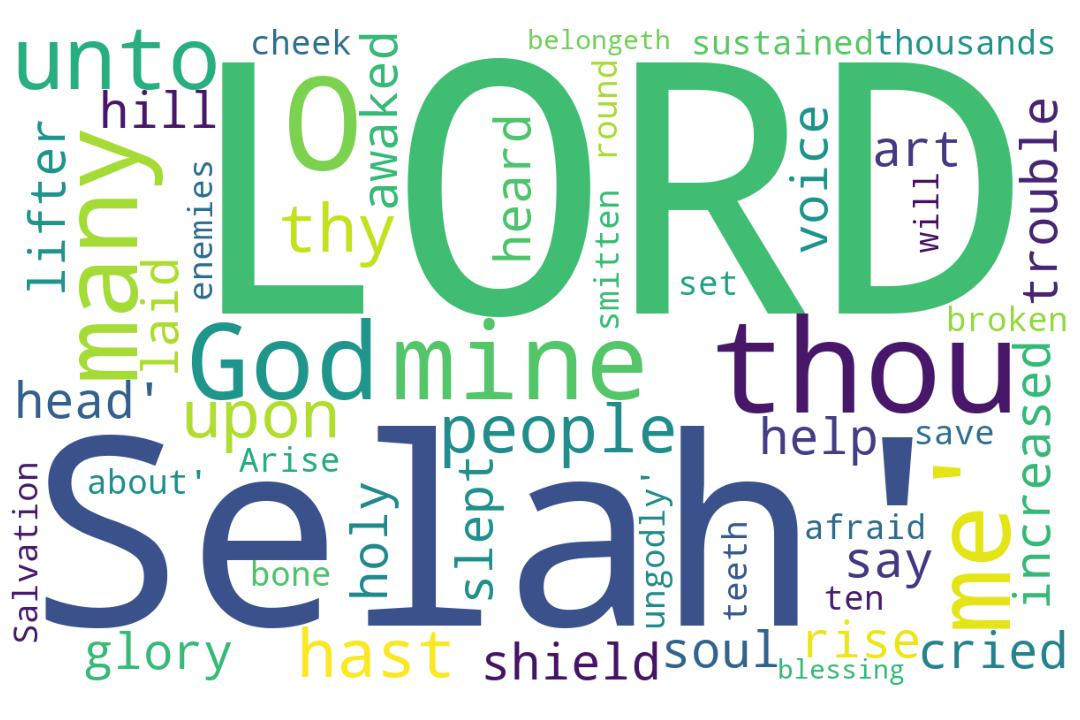
\includegraphics[width=\linewidth]{19OT-Psalms/Psalm3-WordCloud.jpg}
  \caption{Psalm 3 Word Cloud}
  \label{fig:Psalm 3 word Cloud}
\end{figure}

\marginpar{\scriptsize \centering \fcolorbox{bone}{lime}{\textbf{THE LORD, MY HELP}}\\ (Psalm 3:1-8) \begin{compactenum}[I.][8]
	\item A \textbf{Distressed Soul} \index [scripture]{Psalms!Psa 003:02} (Psa 3:2)
	\item A \textbf{Durable Shield} \index [scripture]{Psalms!Psa 003:03} (Psa 3:3)
	\item A \textbf{Defender \& Sustainer} \index[scripture]{Psalms!Psa 003:05} (Psa 3:5)
    \item \textbf{Delightful Sleep} of Peace \index[scripture]{Psalms!Psa 003:05} (Psa 3:5)
    \item One \textbf{Dependable \& Sure} \index[scripture]{Psalms!Psa 003:06} (Psa 3:6)
    \item \textbf{Determined \& Smiting} \index[scripture]{Psalms!Psa 003:07} (Psa 3:7)
   \item  \textbf{Deliverer of Salvation} \index[scripture]{Psalms!Psa 003:08} (Psa 3:8)
\end{compactenum} }

\marginpar{\scriptsize \centering \fcolorbox{bone}{yellow}{\textbf{WHAT GOD DID FOR DAVID}}\\ (Psalm 3:1-8) God:
\begin{compactenum}[I.][8] 
    \item \textbf{God Saw him Surrounded by Enemies} \index[scripture]{Psalms!Psa 003:01} (Psa 3:1)
    \item \textbf{God Secured Him Against Overwhelming Odds} \index[scripture]{Psalms!Psa 003:01} (Psa 3:1)
    \item \textbf{God Sent him Help} \index[scripture]{Psalms!Psa 003:02} (Psa 3:2)
    \item \textbf{God Shielded him from Hurt} \index[scripture]{Psalms!Psa 003:03} (Psa 3:3)
    \item \textbf{God Sustained Him} \index[scripture]{Psalms!Psa 003:05} (Psa 3:5)
    \item \textbf{God Smote the Heathen} \index[scripture]{Psalms!Psa 003:07} (Psa 3:7)
    \item \textbf{God Separated the Teeth of the ungodly} \index[scripture]{Psalms!Psa 003:07} (Psa 3:7)
\end{compactenum} }

\marginpar{\scriptsize \centering \fcolorbox{bone}{black}{\textbf{\textcolor[cmyk]{0,0,0,0}{A TIME OF ANGUISH}}}\\ (Psalm 3) 
\begin{compactenum}[I.]
    \item \textbf{Personal Heartache} - - and heartbreak, but by God's grace and mercy, it was also a time of:
    \item \textbf{Persistent Help} (verses 3, 4, 5, 7)
    \item \textbf{Protected Head} - - God protected both David's physical head and David's throne, the headship as king (verse 3)
    \item A \textbf{Penitential Heart} - - no doubt that David fully realized that Absalom's rebellion, along with many other family problems, results from his sin with Bathsheba. David was never the same after this succession of sin.  He lived with his sorrow.
    \item \textbf{Purifying and Healing} - - there is nothing like God letting us reap the seed we have sown to let us experience his mercy. It is both a purifying and healing process to go through this.  God delivers and cleanses, yet again. 
    \item \textbf{Preserved Honor} - - David gets restored back to the throne, and Absalom is killed by Joab
    \item An \textbf{Ever-Present Hope}
\end{compactenum} }

\marginpar{\scriptsize \centering \fcolorbox{bone}{blue}{\textbf{\textcolor[cmyk]{0,0,0,0}{READYING THE PLACE}}}\\
\fcolorbox{bone}{blue}{\textbf{\textcolor[cmyk]{0,0,0,0}{OF REFUGE}}} \\(Psalm 3) \\
Psalm 3 has the second mention of this word ``Selah''. The first is in 2 Kings 14:7, where it is captured and given the name ``Joktheel.''
\begin{compactenum}[I.]
    \item The \textbf{Capture} - \index[scripture]{2Kings!2Ki 14:07} (2 Kings 14:7)
    \item The \textbf{Coalition} - \index[scripture]{Psalms!Psa 003:01} (Psa 3:1)
    \item The \textbf{Condition} - \index[scripture]{Psalms!Psa 003:02} (Psa 3:2)
    \item The \textbf{Cry} - \index[scripture]{Psalms!Psa 003:04} (Psa 3:4)
    \item The \textbf{Care} - \index[scripture]{Psalms!Psa 003:04} (Psa 3:5)
     \item The \textbf{Conquest} - \index[scripture]{Psalms!Psa 003:07} (Psa 3:7)
   \item The \textbf{Consummation} - \index[scripture]{Psalms!Psa 003:08} (Psa 3:8)
\end{compactenum} }

\footnote{\textcolor[cmyk]{0.99998,1,0,0}{\hyperlink{TOC}{Return to end of Table of Contents.}}}\footnote{\href{https://www.audioverse.org/english/audiobibles/books/ENGKJV/O/Ps/1}{\textcolor[cmyk]{0.99998,1,0,0}{Psalms Audio}}}\textcolor[cmyk]{0.99998,1,0,0}{A Psalm of David, when he fled from Absalom his son.}\\
\\
\textcolor[cmyk]{0.99998,1,0,0}{LORD\textcolor{jungle}{$_{337}$}, how are they increased that trouble me! many \emph{are} they that rise up against me.}
[2] \textcolor[cmyk]{0.99998,1,0,0}{Many\textcolor{jungle}{$_{353}$} \emph{there} \emph{be} which say of my \fcolorbox{bone}{lime}{soul}, \emph{There} \emph{is} no help for him in God. Selah.}
[3] \textcolor[cmyk]{0.99998,1,0,0}{But\textcolor{jungle}{$_{370}$} thou, O LORD, \emph{art} a \fcolorbox{bone}{lime}{shield} for me; my glory, and the lifter up of mine head.}
[4] \textcolor[cmyk]{0.99998,1,0,0}{I\textcolor{jungle}{$_{388}$} cried unto the LORD with my voice, and he heard me out of his holy hill. Selah.}
[5] \textcolor[cmyk]{0.99998,1,0,0}{I\textcolor{jungle}{$_{406}$} laid me down and \fcolorbox{bone}{lime}{slept}; I awaked; for the LORD \fcolorbox{bone}{lime}{sustained} me.}
[6] \textcolor[cmyk]{0.99998,1,0,0}{I\textcolor{jungle}{$_{419}$} will \fcolorbox{bone}{lime}{not} be afraid of ten thousands of people, that have set \emph{themselves} against me round about.}
[7] \textcolor[cmyk]{0.99998,1,0,0}{Arise\textcolor{jungle}{$_{437}$}, O LORD; save me, O my God: for thou hast \fcolorbox{bone}{lime}{smitten} all mine enemies \emph{upon} the cheek bone; thou hast broken the teeth of the ungodly.}
[8] \textcolor[cmyk]{0.99998,1,0,0}{\fcolorbox{bone}{lime}{Salvation}\textcolor{jungle}{$_{464}$} \emph{belongeth} unto the LORD: thy blessing \emph{is} upon thy people. Selah\textcolor{jungle}{$_{475}$}.}



\section{Psalm 3 Comments}




%\index[NWIV]{16!Psalms!Psa 3:1}\index[AWIP]{LORD!Psalms!Psa 3:1}\index[AWIP]{how!Psalms!Psa 3:1}\index[AWIP]{are!Psalms!Psa 3:1}\index[AWIP]{they!Psalms!Psa 3:1}\index[AWIP]{they!Psalms!Psa 3:1 (2)}\index[AWIP]{increased!Psalms!Psa 3:1}\index[AWIP]{that!Psalms!Psa 3:1}\index[AWIP]{that!Psalms!Psa 3:1 (2)}\index[AWIP]{trouble!Psalms!Psa 3:1}\index[AWIP]{me!!Psalms!Psa 3:1}\index[AWIP]{many!Psalms!Psa 3:1}\index[AWIP]{\emph{are}!Psalms!Psa 3:1}\index[AWIP]{rise!Psalms!Psa 3:1}\index[AWIP]{up!Psalms!Psa 3:1}\index[AWIP]{against!Psalms!Psa 3:1}\index[AWIP]{me!Psalms!Psa 3:1}\index[AWIP]{\emph{are}!Psalms!Psa 3:1}

\index[NWIV]{17!Psalms!Psa 3:2}\index[AWIP]{Many!Psalms!Psa 3:2}\index[AWIP]{\emph{there}!Psalms!Psa 3:2}\index[AWIP]{\emph{be}!Psalms!Psa 3:2}\index[AWIP]{which!Psalms!Psa 3:2}\index[AWIP]{say!Psalms!Psa 3:2}\index[AWIP]{of!Psalms!Psa 3:2}\index[AWIP]{my!Psalms!Psa 3:2}\index[AWIP]{soul!Psalms!Psa 3:2}\index[AWIP]{\emph{There}!Psalms!Psa 3:2}\index[AWIP]{\emph{is}!Psalms!Psa 3:2}\index[AWIP]{no!Psalms!Psa 3:2}\index[AWIP]{help!Psalms!Psa 3:2}\index[AWIP]{for!Psalms!Psa 3:2}\index[AWIP]{him!Psalms!Psa 3:2}\index[AWIP]{in!Psalms!Psa 3:2}\index[AWIP]{God!Psalms!Psa 3:2}\index[AWIP]{Selah!Psalms!Psa 3:2}\index[AWIP]{\emph{there}!Psalms!Psa 3:2}\index[AWIP]{\emph{be}!Psalms!Psa 3:2}\index[AWIP]{\emph{There}!Psalms!Psa 3:2}\index[AWIP]{\emph{is}!Psalms!Psa 3:2}

\index[NWIV]{18!Psalms!Psa 3:3}\index[AWIP]{But!Psalms!Psa 3:3}\index[AWIP]{thou!Psalms!Psa 3:3}\index[AWIP]{O!Psalms!Psa 3:3}\index[AWIP]{LORD!Psalms!Psa 3:3}\index[AWIP]{\emph{art}!Psalms!Psa 3:3}\index[AWIP]{a!Psalms!Psa 3:3}\index[AWIP]{shield!Psalms!Psa 3:3}\index[AWIP]{for!Psalms!Psa 3:3}\index[AWIP]{me!Psalms!Psa 3:3}\index[AWIP]{my!Psalms!Psa 3:3}\index[AWIP]{glory!Psalms!Psa 3:3}\index[AWIP]{and!Psalms!Psa 3:3}\index[AWIP]{the!Psalms!Psa 3:3}\index[AWIP]{lifter!Psalms!Psa 3:3}\index[AWIP]{up!Psalms!Psa 3:3}\index[AWIP]{of!Psalms!Psa 3:3}\index[AWIP]{mine!Psalms!Psa 3:3}\index[AWIP]{head!Psalms!Psa 3:3}\index[AWIP]{\emph{art}!Psalms!Psa 3:3}

\index[NWIV]{18!Psalms!Psa 3:4}\index[AWIP]{I!Psalms!Psa 3:4}\index[AWIP]{cried!Psalms!Psa 3:4}\index[AWIP]{unto!Psalms!Psa 3:4}\index[AWIP]{the!Psalms!Psa 3:4}\index[AWIP]{LORD!Psalms!Psa 3:4}\index[AWIP]{with!Psalms!Psa 3:4}\index[AWIP]{my!Psalms!Psa 3:4}\index[AWIP]{voice!Psalms!Psa 3:4}\index[AWIP]{and!Psalms!Psa 3:4}\index[AWIP]{he!Psalms!Psa 3:4}\index[AWIP]{heard!Psalms!Psa 3:4}\index[AWIP]{me!Psalms!Psa 3:4}\index[AWIP]{out!Psalms!Psa 3:4}\index[AWIP]{of!Psalms!Psa 3:4}\index[AWIP]{his!Psalms!Psa 3:4}\index[AWIP]{holy!Psalms!Psa 3:4}\index[AWIP]{hill!Psalms!Psa 3:4}\index[AWIP]{Selah!Psalms!Psa 3:4}

\index[NWIV]{13!Psalms!Psa 3:5}\index[AWIP]{I!Psalms!Psa 3:5}\index[AWIP]{I!Psalms!Psa 3:5 (2)}\index[AWIP]{laid!Psalms!Psa 3:5}\index[AWIP]{me!Psalms!Psa 3:5}\index[AWIP]{me!Psalms!Psa 3:5 (2)}\index[AWIP]{down!Psalms!Psa 3:5}\index[AWIP]{and!Psalms!Psa 3:5}\index[AWIP]{slept!Psalms!Psa 3:5}\index[AWIP]{awaked!Psalms!Psa 3:5}\index[AWIP]{for!Psalms!Psa 3:5}\index[AWIP]{the!Psalms!Psa 3:5}\index[AWIP]{LORD!Psalms!Psa 3:5}\index[AWIP]{sustained!Psalms!Psa 3:5}

\index[NWIV]{18!Psalms!Psa 3:6}\index[AWIP]{I!Psalms!Psa 3:6}\index[AWIP]{will!Psalms!Psa 3:6}\index[AWIP]{not!Psalms!Psa 3:6}\index[AWIP]{be!Psalms!Psa 3:6}\index[AWIP]{afraid!Psalms!Psa 3:6}\index[AWIP]{of!Psalms!Psa 3:6}\index[AWIP]{of!Psalms!Psa 3:6 (2)}\index[AWIP]{ten!Psalms!Psa 3:6}\index[AWIP]{thousands!Psalms!Psa 3:6}\index[AWIP]{people!Psalms!Psa 3:6}\index[AWIP]{that!Psalms!Psa 3:6}\index[AWIP]{have!Psalms!Psa 3:6}\index[AWIP]{set!Psalms!Psa 3:6}\index[AWIP]{\emph{themselves}!Psalms!Psa 3:6}\index[AWIP]{against!Psalms!Psa 3:6}\index[AWIP]{me!Psalms!Psa 3:6}\index[AWIP]{round!Psalms!Psa 3:6}\index[AWIP]{about!Psalms!Psa 3:6}\index[AWIP]{\emph{themselves}!Psalms!Psa 3:6}

\index[NWIV]{27!Psalms!Psa 3:7}\index[AWIP]{Arise!Psalms!Psa 3:7}\index[AWIP]{O!Psalms!Psa 3:7}\index[AWIP]{O!Psalms!Psa 3:7 (2)}\index[AWIP]{LORD!Psalms!Psa 3:7}\index[AWIP]{save!Psalms!Psa 3:7}\index[AWIP]{me!Psalms!Psa 3:7}\index[AWIP]{my!Psalms!Psa 3:7}\index[AWIP]{God!Psalms!Psa 3:7}\index[AWIP]{for!Psalms!Psa 3:7}\index[AWIP]{thou!Psalms!Psa 3:7}\index[AWIP]{thou!Psalms!Psa 3:7 (2)}\index[AWIP]{hast!Psalms!Psa 3:7}\index[AWIP]{hast!Psalms!Psa 3:7 (2)}\index[AWIP]{smitten!Psalms!Psa 3:7}\index[AWIP]{all!Psalms!Psa 3:7}\index[AWIP]{mine!Psalms!Psa 3:7}\index[AWIP]{enemies!Psalms!Psa 3:7}\index[AWIP]{\emph{upon}!Psalms!Psa 3:7}\index[AWIP]{the!Psalms!Psa 3:7}\index[AWIP]{the!Psalms!Psa 3:7 (2)}\index[AWIP]{the!Psalms!Psa 3:7 (3)}\index[AWIP]{cheek!Psalms!Psa 3:7}\index[AWIP]{bone!Psalms!Psa 3:7}\index[AWIP]{broken!Psalms!Psa 3:7}\index[AWIP]{teeth!Psalms!Psa 3:7}\index[AWIP]{of!Psalms!Psa 3:7}\index[AWIP]{ungodly!Psalms!Psa 3:7}\index[AWIP]{\emph{upon}!Psalms!Psa 3:7}

\index[NWIV]{12!Psalms!Psa 3:8}\index[AWIP]{Salvation!Psalms!Psa 3:8}\index[AWIP]{\emph{belongeth}!Psalms!Psa 3:8}\index[AWIP]{unto!Psalms!Psa 3:8}\index[AWIP]{the!Psalms!Psa 3:8}\index[AWIP]{LORD!Psalms!Psa 3:8}\index[AWIP]{thy!Psalms!Psa 3:8}\index[AWIP]{thy!Psalms!Psa 3:8 (2)}\index[AWIP]{blessing!Psalms!Psa 3:8}\index[AWIP]{\emph{is}!Psalms!Psa 3:8}\index[AWIP]{upon!Psalms!Psa 3:8}\index[AWIP]{people!Psalms!Psa 3:8}\index[AWIP]{Selah!Psalms!Psa 3:8}\index[AWIP]{\emph{belongeth}!Psalms!Psa 3:8}\index[AWIP]{\emph{is}!Psalms!Psa 3:8}


\section{Psalm 3 Outlines}

\subsection{My Outlines}

\subsubsection{The Lord, My Help}
\index[speaker]{Keith Anthony!Psalm 003 (The Lord, My Help)}
\index[series]{Psalms (Keith Anthony)!Psalm 003 (The Lord, My Help)}
\index[date]{2014/11/03!Psalm 003 (The Lord, My Help) (Keith Anthony)}

\begin{compactenum}[I.][9]
	\item A \textbf{Distressed Soul} \index [scripture]{Psalms!Psa 003:02} (Psa 3:2)
	\item A \textbf{Durable Shield} \index [scripture]{Psalms!Psa 003:03} (Psa 3:3)
	\item A \textbf{Defender \& Sustainer} \index[scripture]{Psalms!Psa 003:05} (Psa 3:5)
    \item \textbf{The Delightful Sleep} of Peace \index[scripture]{Psalms!Psa 003:05} (Psa 3:5)
    \item One \textbf{Dependable \& Sure} \index[scripture]{Psalms!Psa 003:06} (Psa 3:6)
    \item A \textbf{Determined \& Smiting} \index[scripture]{Psalms!Psa 003:07} (Psa 3:7)
   \item The \textbf{Deliverer of Salvation} \index[scripture]{Psalms!Psa 003:08} (Psa 3:8)
\end{compactenum}

\subsubsection{What God Did for David}

\index[speaker]{Keith Anthony!Psalm 003 (What God Did for David)}
\index[series]{Psalms (Keith Anthony)!Psalm 003 (What God Did for David)}
\index[date]{2014/11/03!Psalm 003 (What God Did for David) (Keith Anthony)}
\textbf{Introduction: }Commentators remind us that Psalm 3 recounts God's protection of David during Absalom's rebellion: 

\begin{compactenum}[I.]
    \item \textbf{God Saw him Surrounded by Enemies} \index[scripture]{Psalms!Psa 003:01} (Psa 3:1)
    \item \textbf{God Secured Him Against Overwhelming Odds} \index[scripture]{Psalms!Psa 003:01} (Psa 3:1)
    \item \textbf{God Sent him Help} \index[scripture]{Psalms!Psa 003:02} (Psa 3:2)
    \item \textbf{God Shielded him from Hurt} \index[scripture]{Psalms!Psa 003:03} (Psa 3:3)
    \item \textbf{God Sustained Him} \index[scripture]{Psalms!Psa 003:05} (Psa 3:5)
    \item \textbf{God Smote the Heathen} \index[scripture]{Psalms!Psa 003:07} (Psa 3:7)
    \item \textbf{God Separated the Teeth of the ungodly} \index[scripture]{Psalms!Psa 003:07} (Psa 3:7)
\end{compactenum}

\subsubsection{A Time of Anguish}
\index[speaker]{Keith Anthony!Psalm 003 (A Time of Anguish)}
\index[series]{Psalms (Keith Anthony)!Psalm 003 (A Time of Anguish)}
\index[date]{2014/11/03!Psalm 003 (A Time of Anguish) (Keith Anthony)}
Commentators remind us that Psalm 3 recounts God's protection of David during Absalom's rebellion. (See the story in 2 Samuel 15:13-17:22). This was a time of: 

\begin{compactenum}[I.]
    \item \textbf{Personal Heartache} - - and heartbreak, but by God's grace and mercy, it was also a time of:
    \item \textbf{Persistent Help} (verses 3, 4, 5, 7)
    \item \textbf{Protected Head} - - God protected both David's physical head and David's throne, the headship as king (verse 3)
    \item A \textbf{Penitential Heart} - - no doubt that David fully realized that Absalom's rebellion, along with many other family problems, results from his sin with Bathsheba. David was never the same after this succession of sin.  He lived with his sorrow.
    \item \textbf{Purifying and Healing} - - there is nothing like God letting us reap the seed we have sown to let us experience his mercy. It is both a purifying and healing process to go through this.  God delivers and cleanses, yet again. 
    \item \textbf{Preserved Honor} - - David gets restored back to the throne, and Absalom is killed by Joab
    \item An \textbf{Ever-Present Hope}
\end{compactenum}


\subsubsection{Readying the Place of Refuge}
\index[speaker]{Keith Anthony!Psalm 003 (Readying the Place of Refuge)}
\index[series]{Psalms (Keith Anthony)!Psalm 003 (Readying the Place of Refuge)}
\index[date]{2021/01/03!Psalm 003 (Readying the Place of Refuge) (Keith Anthony)}

\begin{compactenum}[I.]
    \item The \textbf{Capture} - \index[scripture]{2Kings!2Ki 14:07} (2 Kings 14:7)
    \item The \textbf{Coalition} - \index[scripture]{Psalms!Psa 003:01} (Psa 3:1)
    \item The \textbf{Condition} - \index[scripture]{Psalms!Psa 003:02} (Psa 3:2)
    \item The \textbf{Cry} - \index[scripture]{Psalms!Psa 003:04} (Psa 3:4)
    \item The \textbf{Care} - \index[scripture]{Psalms!Psa 003:04} (Psa 3:5)
     \item The \textbf{Conquest} - \index[scripture]{Psalms!Psa 003:07} (Psa 3:7)
   \item The \textbf{Consummation} - \index[scripture]{Psalms!Psa 003:08} (Psa 3:8)
\end{compactenum} 

\subsection{Outlines from Others}

\subsubsection{David at Mananaim}\footnote{John Phillips}
From John Phillips\cite{Phillips2001ExploringPsalms1}
\begin{compactenum}[I.]
    \item \textbf{David's Trial} (Psalm 3:1-2)
    \begin{compactenum}[A.]
        \item The Multiplicity of His Foes (Psalm 3:1)
        \item The Malignity of His Foes (Psalm 3:1)
    \end{compactenum}
    \item \textbf{David's Trust} (Psalm 3:3-4)
    \begin{compactenum}[A.]
        \item His Assurance in God (Psalm 3:3)
        \item His Appeal to God (Psalm 3:4)
    \end{compactenum}
    \item \textbf{David's Triumph} (Psalm 3:5-8)
    \begin{compactenum}[A.]
        \item David's Vision (Psalm 3:5-6)
        \item David's Victory (Psalm 3:7-8)
    \end{compactenum}
\end{compactenum}
\newpage



%\section{Psalm 3 Statistics}

%%%%%%%%%%%%%%%%%%%%%%%%%%%
%%%%%Word Statistics
%%%%%%%%%%%%%%%%%%%%%%%%%%%


\normalsize



\subsection{Chapter Word Statistics}


%%%%%%%%%%
%%%%%%%%%%
 
\begin{center}
\begin{longtable}{l|c|c|c|c}
\caption[Stats for Psalm 3]{Stats for Psalm 3} \label{table:Stats for Psalm 3} \\ 
\hline \multicolumn{1}{|c|}{\textbf{Verse(s)}} & \multicolumn{1}{|c|}{\textbf{Count}} & \multicolumn{1}{|c|}{\textbf{Unique}} & \multicolumn{1}{|c|}{\textbf{Italics}} & \multicolumn{1}{|c|}{\textbf{Uniq Italic}}  \\ \hline 
\endfirsthead
 
\multicolumn{5}{c}
{{\bfseries \tablename\ \thetable{} -- continued from previous page}} \\  
\hline \multicolumn{1}{|c|}{\textbf{Verse(s)}} & \multicolumn{1}{|c|}{\textbf{Count}} & \multicolumn{1}{|c|}{\textbf{Unique}} & \multicolumn{1}{|c|}{\textbf{Italics}} & \multicolumn{1}{|c|}{\textbf{Uniq Italic}}  \\ \hline 
\endhead
 
\hline \multicolumn{5}{|r|}{{Continued if needed}} \\ \hline
\endfoot 
1 & 16 & 13 & 1 & 1\\ \hline
2 & 17 & 17 & 4 & 4\\ \hline
3 & 18 & 18 & 1 & 1\\ \hline
4 & 18 & 18 & 0 & 0\\ \hline
5 & 13 & 11 & 0 & 0\\ \hline
6 & 18 & 17 & 1 & 1\\ \hline
7 & 27 & 22 & 1 & 1\\ \hline
8 & 12 & 11 & 2 & 2\\ \hline
\hline \hline
Total & 139 & 87 & 10 & 9



\end{longtable}
\end{center}

%%%%%%%%%%
%%%%%%%%%%
 
\subsection{Words by Frequency}

\begin{center}
\begin{longtable}{l|r}
\caption[Word Frequencies in Psalm 3]{Word Frequencies in Psalm 3} \label{table:WordsIn-Psalm-3} \\ 
\hline \multicolumn{1}{|c|}{\textbf{Word}} & \multicolumn{1}{c|}{\textbf{Frequency}} \\ \hline 
\endfirsthead
 
\multicolumn{2}{c}
{{\bfseries \tablename\ \thetable{} -- continued from previous page}} \\ 
\hline \multicolumn{1}{|c|}{\textbf{Word}} & \multicolumn{1}{c|}{\textbf{Frequency}} \\ \hline 
\endhead
 
\hline \multicolumn{2}{|r|}{{Continued if needed}} \\ \hline
\endfoot
 
\hline \hline
\endlastfoot
me & 8 \\ \hline
the & 7 \\ \hline
LORD & 6 \\ \hline
of & 6 \\ \hline
my & 4 \\ \hline
for & 4 \\ \hline
I & 4 \\ \hline
that & 3 \\ \hline
Selah & 3 \\ \hline
thou & 3 \\ \hline
O & 3 \\ \hline
and & 3 \\ \hline
they & 2 \\ \hline
up & 2 \\ \hline
against & 2 \\ \hline
\emph{is} & 2 \\ \hline
God & 2 \\ \hline
mine & 2 \\ \hline
unto & 2 \\ \hline
people & 2 \\ \hline
hast & 2 \\ \hline
thy & 2 \\ \hline
how & 1 \\ \hline
are & 1 \\ \hline
increased & 1 \\ \hline
trouble & 1 \\ \hline
many & 1 \\ \hline
\emph{are} & 1 \\ \hline
rise & 1 \\ \hline
Many & 1 \\ \hline
\emph{there} & 1 \\ \hline
\emph{be} & 1 \\ \hline
which & 1 \\ \hline
say & 1 \\ \hline
soul & 1 \\ \hline
\emph{There} & 1 \\ \hline
no & 1 \\ \hline
help & 1 \\ \hline
him & 1 \\ \hline
in & 1 \\ \hline
But & 1 \\ \hline
\emph{art} & 1 \\ \hline
a & 1 \\ \hline
shield & 1 \\ \hline
glory & 1 \\ \hline
lifter & 1 \\ \hline
head & 1 \\ \hline
cried & 1 \\ \hline
with & 1 \\ \hline
voice & 1 \\ \hline
he & 1 \\ \hline
heard & 1 \\ \hline
out & 1 \\ \hline
his & 1 \\ \hline
holy & 1 \\ \hline
hill & 1 \\ \hline
laid & 1 \\ \hline
down & 1 \\ \hline
slept & 1 \\ \hline
awaked & 1 \\ \hline
sustained & 1 \\ \hline
will & 1 \\ \hline
not & 1 \\ \hline
be & 1 \\ \hline
afraid & 1 \\ \hline
ten & 1 \\ \hline
thousands & 1 \\ \hline
have & 1 \\ \hline
set & 1 \\ \hline
\emph{themselves} & 1 \\ \hline
round & 1 \\ \hline
about & 1 \\ \hline
Arise & 1 \\ \hline
save & 1 \\ \hline
smitten & 1 \\ \hline
all & 1 \\ \hline
enemies & 1 \\ \hline
\emph{upon} & 1 \\ \hline
cheek & 1 \\ \hline
bone & 1 \\ \hline
broken & 1 \\ \hline
teeth & 1 \\ \hline
ungodly & 1 \\ \hline
Salvation & 1 \\ \hline
\emph{belongeth} & 1 \\ \hline
blessing & 1 \\ \hline
upon & 1 \\ \hline
\end{longtable}
\end{center}



\normalsize



\subsection{Words Alphabetically}

\begin{center}
\begin{longtable}{l|r}
\caption[Word Alphabetically in Psalm 3]{Word Alphabetically in Psalm 3} \label{table:WordsIn-Psalm-3} \\ 
\hline \multicolumn{1}{|c|}{\textbf{Word}} & \multicolumn{1}{c|}{\textbf{Frequency}} \\ \hline 
\endfirsthead
 
\multicolumn{2}{c}
{{\bfseries \tablename\ \thetable{} -- continued from previous page}} \\ 
\hline \multicolumn{1}{|c|}{\textbf{Word}} & \multicolumn{1}{c|}{\textbf{Frequency}} \\ \hline 
\endhead
 
\hline \multicolumn{2}{|r|}{{Continued if needed}} \\ \hline
\endfoot
 
\hline \hline
\endlastfoot
Arise & 1 \\ \hline
But & 1 \\ \hline
God & 2 \\ \hline
I & 4 \\ \hline
LORD & 6 \\ \hline
Many & 1 \\ \hline
O & 3 \\ \hline
Salvation & 1 \\ \hline
Selah & 3 \\ \hline
\emph{There} & 1 \\ \hline
\emph{are} & 1 \\ \hline
\emph{art} & 1 \\ \hline
\emph{belongeth} & 1 \\ \hline
\emph{be} & 1 \\ \hline
\emph{is} & 2 \\ \hline
\emph{themselves} & 1 \\ \hline
\emph{there} & 1 \\ \hline
\emph{upon} & 1 \\ \hline
a & 1 \\ \hline
about & 1 \\ \hline
afraid & 1 \\ \hline
against & 2 \\ \hline
all & 1 \\ \hline
and & 3 \\ \hline
are & 1 \\ \hline
awaked & 1 \\ \hline
be & 1 \\ \hline
blessing & 1 \\ \hline
bone & 1 \\ \hline
broken & 1 \\ \hline
cheek & 1 \\ \hline
cried & 1 \\ \hline
down & 1 \\ \hline
enemies & 1 \\ \hline
for & 4 \\ \hline
glory & 1 \\ \hline
hast & 2 \\ \hline
have & 1 \\ \hline
he & 1 \\ \hline
head & 1 \\ \hline
heard & 1 \\ \hline
help & 1 \\ \hline
hill & 1 \\ \hline
him & 1 \\ \hline
his & 1 \\ \hline
holy & 1 \\ \hline
how & 1 \\ \hline
in & 1 \\ \hline
increased & 1 \\ \hline
laid & 1 \\ \hline
lifter & 1 \\ \hline
many & 1 \\ \hline
me & 8 \\ \hline
mine & 2 \\ \hline
my & 4 \\ \hline
no & 1 \\ \hline
not & 1 \\ \hline
of & 6 \\ \hline
out & 1 \\ \hline
people & 2 \\ \hline
rise & 1 \\ \hline
round & 1 \\ \hline
save & 1 \\ \hline
say & 1 \\ \hline
set & 1 \\ \hline
shield & 1 \\ \hline
slept & 1 \\ \hline
smitten & 1 \\ \hline
soul & 1 \\ \hline
sustained & 1 \\ \hline
teeth & 1 \\ \hline
ten & 1 \\ \hline
that & 3 \\ \hline
the & 7 \\ \hline
they & 2 \\ \hline
thou & 3 \\ \hline
thousands & 1 \\ \hline
thy & 2 \\ \hline
trouble & 1 \\ \hline
ungodly & 1 \\ \hline
unto & 2 \\ \hline
up & 2 \\ \hline
upon & 1 \\ \hline
voice & 1 \\ \hline
which & 1 \\ \hline
will & 1 \\ \hline
with & 1 \\ \hline
\end{longtable}
\end{center}



\normalsize



\subsection{Word Lengths in Chapter}
\normalsize
\begin{longtable}{l|p{3.75in}}
\caption[Words by Length in Psalm 3]{Words by Length in Psalm 3} \label{table:WordsIn-Psalm-3} \\ 
\hline \multicolumn{1}{|c|}{\textbf{Length}} & \multicolumn{1}{c|}{\textbf{Words}} \\ \hline 
\endfirsthead
 
\multicolumn{2}{c}
{{\bfseries \tablename\ \thetable{} -- continued from previous page}} \\ 
\hline \multicolumn{1}{|c|}{\textbf{Length}} & \multicolumn{1}{c|}{\textbf{Words}} \\ \hline 
\endhead
 
\hline \multicolumn{2}{|r|}{{Continued if needed}} \\ \hline
\endfoot
 
\hline \hline
\endlastfoot
1 & O, a, I \\ \hline
2 & me, up, \emph{be}, of, my, \emph{is}, no, in, he, be \\ \hline
3 & how, are, \emph{are}, say, for, him, God, But, \emph{art}, and, the, out, his, not, ten, set, all, thy \\ \hline
4 & LORD, they, that, many, rise, Many, soul, help, thou, mine, head, unto, with, holy, hill, laid, down, will, have, save, hast, \emph{upon}, bone, upon \\ \hline
5 & \emph{there}, which, \emph{There}, Selah, glory, cried, voice, heard, slept, round, about, Arise, cheek, teeth \\ \hline
6 & shield, lifter, awaked, afraid, people, broken \\ \hline
7 & trouble, against, smitten, enemies, ungodly \\ \hline
8 & blessing \\ \hline
9 & increased, sustained, thousands, Salvation, \emph{belongeth} \\ \hline
10 & \emph{themselves} \\ \hline
\end{longtable}






%%%%%%%%%%
%%%%%%%%%%
 



%%%%%%%%%%
%%%%%%%%%%
\subsection{Verses with 13 Words in Chapter}
\normalsize
\begin{longtable}{l|p{3.75in}}
\caption[Verses with 13 Words  in Psalm 3]{Verses with 13 Words  in Psalm 3} \label{table:Verses with 13 Words in-Psalm-3} \\ 
\hline \multicolumn{1}{|c|}{\textbf{Reference}} & \multicolumn{1}{c|}{\textbf{Verse}} \\ \hline 
\endfirsthead
 
\multicolumn{2}{c}
{{\bfseries \tablename\ \thetable{} -- continued from previous page}} \\ 
\hline \multicolumn{1}{|c|}{\textbf{Reference}} & \multicolumn{1}{c|}{\textbf{Verse}} \\ \hline 
\endhead
 
\hline \multicolumn{2}{|r|}{{Continued if needed}} \\ \hline
\endfoot
 
\hline \hline
\endlastfoot
Psalms 003:5 & I laid me down and slept; I awaked; for the LORD sustained me. \\ \hline
\end{longtable}






%%%%%%%%%%
%%%%%%%%%%
\subsection{Psalm3 Repeated Phrases}


%%%%%%%%%%
%%%%%%%%%%
\normalsize
 
\begin{center}
\begin{longtable}{|p{3.0in}|p{0.5in}|}
\caption[Psalm3 Repeated Phrases]{Psalm3 Repeated Phrases}\label{table:Repeated Phrases Psalm3} \\
\hline \multicolumn{1}{|c|}{\textbf{Phrase}} & \multicolumn{1}{c|}{\textbf{Frequency}} \\ \hline 
\endfirsthead
 
\multicolumn{2}{c}
{{\bfseries \tablename\ \thetable{} -- continued from previous page}} \\  
\hline \multicolumn{1}{|c|}{\textbf{Phrase}} & \multicolumn{1}{c|}{\textbf{Frequency}} \\ \hline 
\endhead
 
\hline \multicolumn{2}{c}{{ }} \\ \hline
\endfoot 
the LORD & 3\\ \hline 
\end{longtable}
\end{center}



%%%%%%%%%%
%%%%%%%%%%




\chapter{Psalm 4}

\begin{figure}
  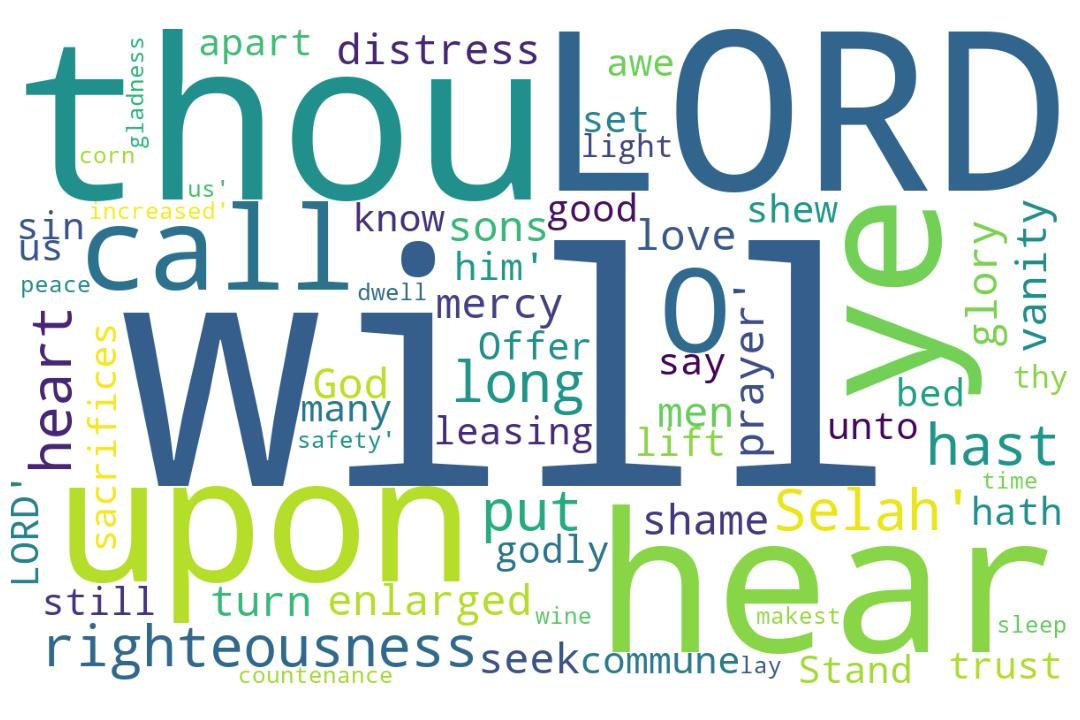
\includegraphics[width=\linewidth]{19OT-Psalms/Psalm4-WordCloud.jpg}
  \caption{Psalm 4 Word Cloud}
  \label{fig:Psalm 4 word Cloud}
\end{figure}

\marginpar{\scriptsize \centering \fcolorbox{bone}{lime}{\textbf{CONFIDENCE IN GOD}}\\ (Psalm 4) 
\begin{compactenum}[I.][8]
    \item \textbf{Consideration of God's Enemies} \index[scripture]{Psalms!Psa 004:01}(Psa 4:1)
    \item \textbf{Call to the Faithful One} \index[scripture]{Psalms!Psa 004:01}(Psa 4:1)
    \item \textbf{Confidence in God's Way} \index[scripture]{Psalms!Psa 004:01}(Psa 4:1)
    \item \textbf{Contentment in Heart} \index[scripture]{Psalms!Psa 004:07}(Psa 4:7)
    \item \textbf{Countenance Provided} \index[scripture]{Psalms!Psa 004:06}(Psa 4:6)
    \item \textbf{Confirmation of Presence} \index[scripture]{Psalms!Psa 004:08}(Psa 4:8)
    \item \textbf{Calmness and Peace} \index[scripture]{Psalms!Psa 004:08}(Psa 4:8)
\end{compactenum} } 

\marginpar{\scriptsize \centering \fcolorbox{bone}{yellow}{\textbf{THE MINISTRY OF LIES}}\\ (Psalm 4) 
\begin{compactenum}[I.][8]
	\item  \textbf{Insincere Boldness} -- Do you take a hard stand against something, but in  the details, one could see small compromises on the same issue
	\item \textbf{Imperfect Book} -- Do you really have a perfect book? Do you actually believe  the WORDS that it says?
	\item \textbf{Impure Bride} -- what ``little sins'' of convenience do you overlook (most likely, non-Christians are not overlooking them)
	\item \textbf{Insincere Brethren} -- Don't pretend to care, if you don't $\hdots$  don't say you pray or will pray when you don't or won't $\hdots$ And why do you not care  anyway?
	\item \textbf{Inordinate Bonds} - (Ezekiel 23:11) Who or what are you beholden to? Who are you secretly trying to be like?
	\item \textbf{Inconsistent Beliefs} -- How much or your beliefs actually are not scriptural? And how would you react when someone showed you?
	\item \textbf{Invisible Blessings} -- if you say you are a Christian, who are you being a blessing to?
	\item A\textbf{(Mis)Interpreted Bible} -- Do  you REALLY understand the Bible, or just take the word of the guy in the pulpit?
\end{compactenum} }

\footnote{\textcolor[cmyk]{0.99998,1,0,0}{\hyperlink{TOC}{Return to end of Table of Contents.}}}\footnote{\href{https://audiobible.com/bible/bible.html}{\textcolor[cmyk]{0.99998,1,0,0}{Psalms Audio}}}\textcolor[cmyk]{0.99998,1,0,0}{To the chief Musician on Neginoth, A Psalm of David.}\\
\\
\textcolor[cmyk]{0.99998,1,0,0}{Hear\textcolor{jungle}{$_{476}$} me when I \fcolorbox{bone}{lime}{call}, O \fcolorbox{bone}{lime}{God of my righteousness}: thou hast enlarged me \emph{when} \emph{I} \emph{was} in distress; have mercy upon me, and hear my prayer.}
[2] \textcolor[cmyk]{0.99998,1,0,0}{O\textcolor{jungle}{$_{503}$} ye sons of men, how long \emph{will} \emph{ye} \emph{turn} my glory into shame? \emph{how} \emph{long} will ye love vanity, \emph{and} seek after leasing? Selah.}
[3] \textcolor[cmyk]{0.99998,1,0,0}{But\textcolor{jungle}{$_{528}$} know that the LORD hath set apart him that is godly for himself: the LORD will hear when I call unto him.}
[4] \textcolor[cmyk]{0.99998,1,0,0}{Stand\textcolor{jungle}{$_{551}$} in awe, and sin not: commune with your own heart upon your bed, and be still. Selah.}
[5] \textcolor[cmyk]{0.99998,1,0,0}{Offer\textcolor{jungle}{$_{569}$} the sacrifices of righteousness, and put your trust in the LORD.}\footnote{\textbf{Deuteronomy 33:19} - They shall call the people unto the mountain; there they shall offer sacrifices of righteousness: for they shall suck of the abundance of the seas, and of treasures hid in the sand.}\footnote{\textbf{Psalm 51:19} - Then shalt thou be pleased with the sacrifices of righteousness, with burnt offering and whole burnt offering: then shall they offer bullocks upon thine altar.}
[6] \textcolor[cmyk]{0.99998,1,0,0}{\emph{There}\textcolor{jungle}{$_{581}$} \emph{be} many that say, Who will shew us \emph{any} good? LORD, lift thou up the light of thy \fcolorbox{bone}{lime}{countenance} upon us.}
[7] \textcolor[cmyk]{0.99998,1,0,0}{Thou\textcolor{jungle}{$_{603}$} hast put \fcolorbox{bone}{lime}{gladness in my heart}, more than in the time \emph{that} their corn and their wine increased.}
[8] \textcolor[cmyk]{0.99998,1,0,0}{I\textcolor{jungle}{$_{622}$} will both lay me down \fcolorbox{bone}{lime}{in peace}, and sleep: for thou, LORD, only makest me dwell \fcolorbox{bone}{lime}{in safety}\textcolor{jungle}{$_{640}$}.}




\section{Psalm 4 Comments}

\subsection{NUmeric Nuggets}
\textbf{13:} There are 13 words in italics in the psalm.

%\index[NWIV]{27!Psalms!Psa 4:1}\index[AWIP]{Hear!Psalms!Psa 4:1}\index[AWIP]{me!Psalms!Psa 4:1}\index[AWIP]{me!Psalms!Psa 4:1 (2)}\index[AWIP]{me!Psalms!Psa 4:1 (3)}\index[AWIP]{when!Psalms!Psa 4:1}\index[AWIP]{I!Psalms!Psa 4:1}\index[AWIP]{call!Psalms!Psa 4:1}\index[AWIP]{O!Psalms!Psa 4:1}\index[AWIP]{God!Psalms!Psa 4:1}\index[AWIP]{of!Psalms!Psa 4:1}\index[AWIP]{my!Psalms!Psa 4:1}\index[AWIP]{my!Psalms!Psa 4:1 (2)}\index[AWIP]{righteousness!Psalms!Psa 4:1}\index[AWIP]{thou!Psalms!Psa 4:1}\index[AWIP]{hast!Psalms!Psa 4:1}\index[AWIP]{enlarged!Psalms!Psa 4:1}\index[AWIP]{\emph{when}!Psalms!Psa 4:1}\index[AWIP]{\emph{I}!Psalms!Psa 4:1}\index[AWIP]{\emph{was}!Psalms!Psa 4:1}\index[AWIP]{in!Psalms!Psa 4:1}\index[AWIP]{distress!Psalms!Psa 4:1}\index[AWIP]{have!Psalms!Psa 4:1}\index[AWIP]{mercy!Psalms!Psa 4:1}\index[AWIP]{upon!Psalms!Psa 4:1}\index[AWIP]{and!Psalms!Psa 4:1}\index[AWIP]{hear!Psalms!Psa 4:1}\index[AWIP]{prayer!Psalms!Psa 4:1}\index[AWIP]{\emph{when}!Psalms!Psa 4:1}\index[AWIP]{\emph{I}!Psalms!Psa 4:1}\index[AWIP]{\emph{was}!Psalms!Psa 4:1}

\index[NWIV]{25!Psalms!Psa 4:2}\index[AWIP]{O!Psalms!Psa 4:2}\index[AWIP]{ye!Psalms!Psa 4:2}\index[AWIP]{ye!Psalms!Psa 4:2 (2)}\index[AWIP]{sons!Psalms!Psa 4:2}\index[AWIP]{of!Psalms!Psa 4:2}\index[AWIP]{men!Psalms!Psa 4:2}\index[AWIP]{how!Psalms!Psa 4:2}\index[AWIP]{long!Psalms!Psa 4:2}\index[AWIP]{\emph{will}!Psalms!Psa 4:2}\index[AWIP]{\emph{ye}!Psalms!Psa 4:2}\index[AWIP]{\emph{turn}!Psalms!Psa 4:2}\index[AWIP]{my!Psalms!Psa 4:2}\index[AWIP]{glory!Psalms!Psa 4:2}\index[AWIP]{into!Psalms!Psa 4:2}\index[AWIP]{shame?!Psalms!Psa 4:2}\index[AWIP]{\emph{how}!Psalms!Psa 4:2}\index[AWIP]{\emph{long}!Psalms!Psa 4:2}\index[AWIP]{will!Psalms!Psa 4:2}\index[AWIP]{love!Psalms!Psa 4:2}\index[AWIP]{vanity!Psalms!Psa 4:2}\index[AWIP]{\emph{and}!Psalms!Psa 4:2}\index[AWIP]{seek!Psalms!Psa 4:2}\index[AWIP]{after!Psalms!Psa 4:2}\index[AWIP]{leasing?!Psalms!Psa 4:2}\index[AWIP]{Selah!Psalms!Psa 4:2}\index[AWIP]{\emph{will}!Psalms!Psa 4:2}\index[AWIP]{\emph{ye}!Psalms!Psa 4:2}\index[AWIP]{\emph{turn}!Psalms!Psa 4:2}\index[AWIP]{\emph{how}!Psalms!Psa 4:2}\index[AWIP]{\emph{long}!Psalms!Psa 4:2}\index[AWIP]{\emph{and}!Psalms!Psa 4:2}

\index[NWIV]{23!Psalms!Psa 4:3}\index[AWIP]{But!Psalms!Psa 4:3}\index[AWIP]{know!Psalms!Psa 4:3}\index[AWIP]{that!Psalms!Psa 4:3}\index[AWIP]{that!Psalms!Psa 4:3 (2)}\index[AWIP]{the!Psalms!Psa 4:3}\index[AWIP]{the!Psalms!Psa 4:3 (2)}\index[AWIP]{LORD!Psalms!Psa 4:3}\index[AWIP]{LORD!Psalms!Psa 4:3 (2)}\index[AWIP]{hath!Psalms!Psa 4:3}\index[AWIP]{set!Psalms!Psa 4:3}\index[AWIP]{apart!Psalms!Psa 4:3}\index[AWIP]{him!Psalms!Psa 4:3}\index[AWIP]{him!Psalms!Psa 4:3 (2)}\index[AWIP]{is!Psalms!Psa 4:3}\index[AWIP]{godly!Psalms!Psa 4:3}\index[AWIP]{for!Psalms!Psa 4:3}\index[AWIP]{himself!Psalms!Psa 4:3}\index[AWIP]{will!Psalms!Psa 4:3}\index[AWIP]{hear!Psalms!Psa 4:3}\index[AWIP]{when!Psalms!Psa 4:3}\index[AWIP]{I!Psalms!Psa 4:3}\index[AWIP]{call!Psalms!Psa 4:3}\index[AWIP]{unto!Psalms!Psa 4:3}

\index[NWIV]{18!Psalms!Psa 4:4}\index[AWIP]{Stand!Psalms!Psa 4:4}\index[AWIP]{in!Psalms!Psa 4:4}\index[AWIP]{awe!Psalms!Psa 4:4}\index[AWIP]{and!Psalms!Psa 4:4}\index[AWIP]{and!Psalms!Psa 4:4 (2)}\index[AWIP]{sin!Psalms!Psa 4:4}\index[AWIP]{not!Psalms!Psa 4:4}\index[AWIP]{commune!Psalms!Psa 4:4}\index[AWIP]{with!Psalms!Psa 4:4}\index[AWIP]{your!Psalms!Psa 4:4}\index[AWIP]{your!Psalms!Psa 4:4 (2)}\index[AWIP]{own!Psalms!Psa 4:4}\index[AWIP]{heart!Psalms!Psa 4:4}\index[AWIP]{upon!Psalms!Psa 4:4}\index[AWIP]{bed!Psalms!Psa 4:4}\index[AWIP]{be!Psalms!Psa 4:4}\index[AWIP]{still!Psalms!Psa 4:4}\index[AWIP]{Selah!Psalms!Psa 4:4}

\index[NWIV]{12!Psalms!Psa 4:5}\index[AWIP]{Offer!Psalms!Psa 4:5}\index[AWIP]{the!Psalms!Psa 4:5}\index[AWIP]{the!Psalms!Psa 4:5 (2)}\index[AWIP]{sacrifices!Psalms!Psa 4:5}\index[AWIP]{of!Psalms!Psa 4:5}\index[AWIP]{righteousness!Psalms!Psa 4:5}\index[AWIP]{and!Psalms!Psa 4:5}\index[AWIP]{put!Psalms!Psa 4:5}\index[AWIP]{your!Psalms!Psa 4:5}\index[AWIP]{trust!Psalms!Psa 4:5}\index[AWIP]{in!Psalms!Psa 4:5}\index[AWIP]{LORD!Psalms!Psa 4:5}

\index[NWIV]{22!Psalms!Psa 4:6}\index[AWIP]{\emph{There}!Psalms!Psa 4:6}\index[AWIP]{\emph{be}!Psalms!Psa 4:6}\index[AWIP]{many!Psalms!Psa 4:6}\index[AWIP]{that!Psalms!Psa 4:6}\index[AWIP]{say!Psalms!Psa 4:6}\index[AWIP]{Who!Psalms!Psa 4:6}\index[AWIP]{will!Psalms!Psa 4:6}\index[AWIP]{shew!Psalms!Psa 4:6}\index[AWIP]{us!Psalms!Psa 4:6}\index[AWIP]{us!Psalms!Psa 4:6 (2)}\index[AWIP]{\emph{any}!Psalms!Psa 4:6}\index[AWIP]{good?!Psalms!Psa 4:6}\index[AWIP]{LORD!Psalms!Psa 4:6}\index[AWIP]{lift!Psalms!Psa 4:6}\index[AWIP]{thou!Psalms!Psa 4:6}\index[AWIP]{up!Psalms!Psa 4:6}\index[AWIP]{the!Psalms!Psa 4:6}\index[AWIP]{light!Psalms!Psa 4:6}\index[AWIP]{of!Psalms!Psa 4:6}\index[AWIP]{thy!Psalms!Psa 4:6}\index[AWIP]{countenance!Psalms!Psa 4:6}\index[AWIP]{upon!Psalms!Psa 4:6}\index[AWIP]{\emph{There}!Psalms!Psa 4:6}\index[AWIP]{\emph{be}!Psalms!Psa 4:6}\index[AWIP]{\emph{any}!Psalms!Psa 4:6}

\index[NWIV]{19!Psalms!Psa 4:7}\index[AWIP]{Thou!Psalms!Psa 4:7}\index[AWIP]{hast!Psalms!Psa 4:7}\index[AWIP]{put!Psalms!Psa 4:7}\index[AWIP]{gladness!Psalms!Psa 4:7}\index[AWIP]{in!Psalms!Psa 4:7}\index[AWIP]{in!Psalms!Psa 4:7 (2)}\index[AWIP]{my!Psalms!Psa 4:7}\index[AWIP]{heart!Psalms!Psa 4:7}\index[AWIP]{more!Psalms!Psa 4:7}\index[AWIP]{than!Psalms!Psa 4:7}\index[AWIP]{the!Psalms!Psa 4:7}\index[AWIP]{time!Psalms!Psa 4:7}\index[AWIP]{\emph{that}!Psalms!Psa 4:7}\index[AWIP]{their!Psalms!Psa 4:7}\index[AWIP]{their!Psalms!Psa 4:7 (2)}\index[AWIP]{corn!Psalms!Psa 4:7}\index[AWIP]{and!Psalms!Psa 4:7}\index[AWIP]{wine!Psalms!Psa 4:7}\index[AWIP]{increased!Psalms!Psa 4:7}\index[AWIP]{\emph{that}!Psalms!Psa 4:7}

\index[NWIV]{19!Psalms!Psa 4:8}\index[AWIP]{I!Psalms!Psa 4:8}\index[AWIP]{will!Psalms!Psa 4:8}\index[AWIP]{both!Psalms!Psa 4:8}\index[AWIP]{lay!Psalms!Psa 4:8}\index[AWIP]{me!Psalms!Psa 4:8}\index[AWIP]{me!Psalms!Psa 4:8 (2)}\index[AWIP]{down!Psalms!Psa 4:8}\index[AWIP]{in!Psalms!Psa 4:8}\index[AWIP]{in!Psalms!Psa 4:8 (2)}\index[AWIP]{peace!Psalms!Psa 4:8}\index[AWIP]{and!Psalms!Psa 4:8}\index[AWIP]{sleep!Psalms!Psa 4:8}\index[AWIP]{for!Psalms!Psa 4:8}\index[AWIP]{thou!Psalms!Psa 4:8}\index[AWIP]{LORD!Psalms!Psa 4:8}\index[AWIP]{only!Psalms!Psa 4:8}\index[AWIP]{makest!Psalms!Psa 4:8}\index[AWIP]{dwell!Psalms!Psa 4:8}\index[AWIP]{safety!Psalms!Psa 4:8}


\section{Psalm 4 Outlines}

\subsection{My Outlines}

\subsubsection{Confidence in God}

\index[speaker]{Keith Anthony!Psalm 004 (Confidence in God)}
\index[series]{Psalms (Keith Anthony)!Psalm 004 (Confidence in God)}
\index[date]{unknown!Psalm 004 (Confidence in God) (Keith Anthony)}
\begin{compactenum}[I.]
    \item \textbf{Consideration of God's Enemies} \index[scripture]{Psalms!Psa 004:01}(Psa 4:1)
    \item \textbf{Call to the Faithful One} \index[scripture]{Psalms!Psa 004:01}(Psa 4:1)
    \item \textbf{Confidence in God's Way} \index[scripture]{Psalms!Psa 004:01}(Psa 4:1)
    \item \textbf{Contentment in Heart} \index[scripture]{Psalms!Psa 004:07}(Psa 4:7)
    \item \textbf{Countenance Provided} \index[scripture]{Psalms!Psa 004:06}(Psa 4:6)
    \item \textbf{Confirmation of Presence} \index[scripture]{Psalms!Psa 004:08}(Psa 4:8)
    \item \textbf{Calmness and Peace} \index[scripture]{Psalms!Psa 004:08}(Psa 4:8)
\end{compactenum}

\subsubsection{The Ministry of Lies}

\index[speaker]{Keith Anthony!Psalm 004 (The Ministry of Lies)}
\index[series]{Psalms (Keith Anthony)!Psalm 004 (The Ministry of Lies)}
\index[date]{Keith Anthony!Psalm 004 (The Ministry of Lies) (Keith Anthony)}
\begin{compactenum}[I.]
	\item  \textbf{Insincere Boldness} -- Do you take a hard stand against something, but in  the details, one could see small compromises on the same issue
	\item \textbf{Imperfect Book} -- Do you really have a perfect book? Do you actually believe  the WORDS that it says?
	\item \textbf{Impure Bride} -- what ``little sins'' of convenience do you overlook (most likely, non-Christians are not overlooking them)
	\item \textbf{Insincere Brethren} -- Don't pretend to care, if you don't $\hdots$  don't say you pray or will pray when you don't or won't $\hdots$ And why do you not care  anyway?
	\item \textbf{Inordinate Bonds} - (Ezekiel 23:11) Who or what are you beholden to? Who are you secretly trying to be like?
	\item \textbf{Inconsistent Beliefs} -- How much or your beliefs actually are not scriptural? And how would you react when someone showed you?
	\item \textbf{Invisible Blessings} -- if you say you are a Christian, who are you being a blessing to?
	\item A\textbf{(Mis)Interpreted Bible} -- Do  you REALLY understand the Bible, or just take the word of the guy in the pulpit?
\end{compactenum}


\subsection{Outlines from Others}

%    \item God has prayers \textbf{Directed} to Him \index[scripture]{Psalms!Psa 005:03}(Psalm 5:3) 

%\section{Psalm 4 Statistics}

%%%%%%%%%%%%%%%%%%%%%%%%%%%
%%%%%Word Statistics
%%%%%%%%%%%%%%%%%%%%%%%%%%%


\normalsize



\subsection{Chapter Word Statistics}


%%%%%%%%%%
%%%%%%%%%%
 
\begin{center}
\begin{longtable}{l|c|c|c|c}
\caption[Stats for Psalm 4]{Stats for Psalm 4} \label{table:Stats for Psalm 4} \\ 
\hline \multicolumn{1}{|c|}{\textbf{Verse(s)}} & \multicolumn{1}{|c|}{\textbf{Count}} & \multicolumn{1}{|c|}{\textbf{Unique}} & \multicolumn{1}{|c|}{\textbf{Italics}} & \multicolumn{1}{|c|}{\textbf{Uniq Italic}}  \\ \hline 
\endfirsthead
 
\multicolumn{5}{c}
{{\bfseries \tablename\ \thetable{} -- continued from previous page}} \\  
\hline \multicolumn{1}{|c|}{\textbf{Verse(s)}} & \multicolumn{1}{|c|}{\textbf{Count}} & \multicolumn{1}{|c|}{\textbf{Unique}} & \multicolumn{1}{|c|}{\textbf{Italics}} & \multicolumn{1}{|c|}{\textbf{Uniq Italic}}  \\ \hline 
\endhead
 
\hline \multicolumn{5}{|r|}{{Continued if needed}} \\ \hline
\endfoot 
1 & 27 & 24 & 3 & 3\\ \hline
2 & 25 & 24 & 6 & 6\\ \hline
3 & 23 & 19 & 0 & 0\\ \hline
4 & 18 & 16 & 0 & 0\\ \hline
5 & 12 & 11 & 0 & 0\\ \hline
6 & 22 & 21 & 3 & 3\\ \hline
7 & 19 & 17 & 1 & 1\\ \hline
8 & 19 & 17 & 0 & 0\\ \hline
\hline \hline
Total & 165 & 108 & 13 & 13



\end{longtable}
\end{center}

%%%%%%%%%%
%%%%%%%%%%
 
\subsection{Words by Frequency}

\begin{center}
\begin{longtable}{l|r}
\caption[Word Frequencies in Psalm 4]{Word Frequencies in Psalm 4} \label{table:WordsIn-Psalm-4} \\ 
\hline \multicolumn{1}{|c|}{\textbf{Word}} & \multicolumn{1}{c|}{\textbf{Frequency}} \\ \hline 
\endfirsthead
 
\multicolumn{2}{c}
{{\bfseries \tablename\ \thetable{} -- continued from previous page}} \\ 
\hline \multicolumn{1}{|c|}{\textbf{Word}} & \multicolumn{1}{c|}{\textbf{Frequency}} \\ \hline 
\endhead
 
\hline \multicolumn{2}{|r|}{{Continued if needed}} \\ \hline
\endfoot
 
\hline \hline
\endlastfoot
in & 7 \\ \hline
and & 6 \\ \hline
the & 6 \\ \hline
me & 5 \\ \hline
LORD & 5 \\ \hline
of & 4 \\ \hline
my & 4 \\ \hline
will & 4 \\ \hline
I & 3 \\ \hline
thou & 3 \\ \hline
upon & 3 \\ \hline
that & 3 \\ \hline
your & 3 \\ \hline
when & 2 \\ \hline
call & 2 \\ \hline
O & 2 \\ \hline
righteousness & 2 \\ \hline
hast & 2 \\ \hline
hear & 2 \\ \hline
ye & 2 \\ \hline
Selah & 2 \\ \hline
him & 2 \\ \hline
for & 2 \\ \hline
heart & 2 \\ \hline
put & 2 \\ \hline
us & 2 \\ \hline
their & 2 \\ \hline
Hear & 1 \\ \hline
God & 1 \\ \hline
enlarged & 1 \\ \hline
\emph{when} & 1 \\ \hline
\emph{I} & 1 \\ \hline
\emph{was} & 1 \\ \hline
distress & 1 \\ \hline
have & 1 \\ \hline
mercy & 1 \\ \hline
prayer & 1 \\ \hline
sons & 1 \\ \hline
men & 1 \\ \hline
how & 1 \\ \hline
long & 1 \\ \hline
\emph{will} & 1 \\ \hline
\emph{ye} & 1 \\ \hline
\emph{turn} & 1 \\ \hline
glory & 1 \\ \hline
into & 1 \\ \hline
shame & 1 \\ \hline
\emph{how} & 1 \\ \hline
\emph{long} & 1 \\ \hline
love & 1 \\ \hline
vanity & 1 \\ \hline
\emph{and} & 1 \\ \hline
seek & 1 \\ \hline
after & 1 \\ \hline
leasing & 1 \\ \hline
But & 1 \\ \hline
know & 1 \\ \hline
hath & 1 \\ \hline
set & 1 \\ \hline
apart & 1 \\ \hline
is & 1 \\ \hline
godly & 1 \\ \hline
himself & 1 \\ \hline
unto & 1 \\ \hline
Stand & 1 \\ \hline
awe & 1 \\ \hline
sin & 1 \\ \hline
not & 1 \\ \hline
commune & 1 \\ \hline
with & 1 \\ \hline
own & 1 \\ \hline
bed & 1 \\ \hline
be & 1 \\ \hline
still & 1 \\ \hline
Offer & 1 \\ \hline
sacrifices & 1 \\ \hline
trust & 1 \\ \hline
\emph{There} & 1 \\ \hline
\emph{be} & 1 \\ \hline
many & 1 \\ \hline
say & 1 \\ \hline
Who & 1 \\ \hline
shew & 1 \\ \hline
\emph{any} & 1 \\ \hline
good & 1 \\ \hline
lift & 1 \\ \hline
up & 1 \\ \hline
light & 1 \\ \hline
thy & 1 \\ \hline
countenance & 1 \\ \hline
Thou & 1 \\ \hline
gladness & 1 \\ \hline
more & 1 \\ \hline
than & 1 \\ \hline
time & 1 \\ \hline
\emph{that} & 1 \\ \hline
corn & 1 \\ \hline
wine & 1 \\ \hline
increased & 1 \\ \hline
both & 1 \\ \hline
lay & 1 \\ \hline
down & 1 \\ \hline
peace & 1 \\ \hline
sleep & 1 \\ \hline
only & 1 \\ \hline
makest & 1 \\ \hline
dwell & 1 \\ \hline
safety & 1 \\ \hline
\end{longtable}
\end{center}



\normalsize



\subsection{Words Alphabetically}

\begin{center}
\begin{longtable}{l|r}
\caption[Word Alphabetically in Psalm 4]{Word Alphabetically in Psalm 4} \label{table:WordsIn-Psalm-4} \\ 
\hline \multicolumn{1}{|c|}{\textbf{Word}} & \multicolumn{1}{c|}{\textbf{Frequency}} \\ \hline 
\endfirsthead
 
\multicolumn{2}{c}
{{\bfseries \tablename\ \thetable{} -- continued from previous page}} \\ 
\hline \multicolumn{1}{|c|}{\textbf{Word}} & \multicolumn{1}{c|}{\textbf{Frequency}} \\ \hline 
\endhead
 
\hline \multicolumn{2}{|r|}{{Continued if needed}} \\ \hline
\endfoot
 
\hline \hline
\endlastfoot
But & 1 \\ \hline
God & 1 \\ \hline
Hear & 1 \\ \hline
I & 3 \\ \hline
LORD & 5 \\ \hline
O & 2 \\ \hline
Offer & 1 \\ \hline
Selah & 2 \\ \hline
Stand & 1 \\ \hline
Thou & 1 \\ \hline
Who & 1 \\ \hline
\emph{I} & 1 \\ \hline
\emph{There} & 1 \\ \hline
\emph{and} & 1 \\ \hline
\emph{any} & 1 \\ \hline
\emph{be} & 1 \\ \hline
\emph{how} & 1 \\ \hline
\emph{long} & 1 \\ \hline
\emph{that} & 1 \\ \hline
\emph{turn} & 1 \\ \hline
\emph{was} & 1 \\ \hline
\emph{when} & 1 \\ \hline
\emph{will} & 1 \\ \hline
\emph{ye} & 1 \\ \hline
after & 1 \\ \hline
and & 6 \\ \hline
apart & 1 \\ \hline
awe & 1 \\ \hline
be & 1 \\ \hline
bed & 1 \\ \hline
both & 1 \\ \hline
call & 2 \\ \hline
commune & 1 \\ \hline
corn & 1 \\ \hline
countenance & 1 \\ \hline
distress & 1 \\ \hline
down & 1 \\ \hline
dwell & 1 \\ \hline
enlarged & 1 \\ \hline
for & 2 \\ \hline
gladness & 1 \\ \hline
glory & 1 \\ \hline
godly & 1 \\ \hline
good & 1 \\ \hline
hast & 2 \\ \hline
hath & 1 \\ \hline
have & 1 \\ \hline
hear & 2 \\ \hline
heart & 2 \\ \hline
him & 2 \\ \hline
himself & 1 \\ \hline
how & 1 \\ \hline
in & 7 \\ \hline
increased & 1 \\ \hline
into & 1 \\ \hline
is & 1 \\ \hline
know & 1 \\ \hline
lay & 1 \\ \hline
leasing & 1 \\ \hline
lift & 1 \\ \hline
light & 1 \\ \hline
long & 1 \\ \hline
love & 1 \\ \hline
makest & 1 \\ \hline
many & 1 \\ \hline
me & 5 \\ \hline
men & 1 \\ \hline
mercy & 1 \\ \hline
more & 1 \\ \hline
my & 4 \\ \hline
not & 1 \\ \hline
of & 4 \\ \hline
only & 1 \\ \hline
own & 1 \\ \hline
peace & 1 \\ \hline
prayer & 1 \\ \hline
put & 2 \\ \hline
righteousness & 2 \\ \hline
sacrifices & 1 \\ \hline
safety & 1 \\ \hline
say & 1 \\ \hline
seek & 1 \\ \hline
set & 1 \\ \hline
shame & 1 \\ \hline
shew & 1 \\ \hline
sin & 1 \\ \hline
sleep & 1 \\ \hline
sons & 1 \\ \hline
still & 1 \\ \hline
than & 1 \\ \hline
that & 3 \\ \hline
the & 6 \\ \hline
their & 2 \\ \hline
thou & 3 \\ \hline
thy & 1 \\ \hline
time & 1 \\ \hline
trust & 1 \\ \hline
unto & 1 \\ \hline
up & 1 \\ \hline
upon & 3 \\ \hline
us & 2 \\ \hline
vanity & 1 \\ \hline
when & 2 \\ \hline
will & 4 \\ \hline
wine & 1 \\ \hline
with & 1 \\ \hline
ye & 2 \\ \hline
your & 3 \\ \hline
\end{longtable}
\end{center}



\normalsize



\subsection{Word Lengths in Chapter}
\normalsize
\begin{longtable}{l|p{3.75in}}
\caption[Words by Length in Psalm 4]{Words by Length in Psalm 4} \label{table:WordsIn-Psalm-4} \\ 
\hline \multicolumn{1}{|c|}{\textbf{Length}} & \multicolumn{1}{c|}{\textbf{Words}} \\ \hline 
\endfirsthead
 
\multicolumn{2}{c}
{{\bfseries \tablename\ \thetable{} -- continued from previous page}} \\ 
\hline \multicolumn{1}{|c|}{\textbf{Length}} & \multicolumn{1}{c|}{\textbf{Words}} \\ \hline 
\endhead
 
\hline \multicolumn{2}{|r|}{{Continued if needed}} \\ \hline
\endfoot
 
\hline \hline
\endlastfoot
1 & I, O, \emph{I} \\ \hline
2 & me, of, my, in, ye, \emph{ye}, is, be, \emph{be}, us, up \\ \hline
3 & God, \emph{was}, and, men, how, \emph{how}, \emph{and}, But, the, set, him, for, awe, sin, not, own, bed, put, say, Who, \emph{any}, thy, lay \\ \hline
4 & Hear, when, call, thou, hast, \emph{when}, have, upon, hear, sons, long, \emph{will}, \emph{turn}, into, \emph{long}, will, love, seek, know, that, LORD, hath, unto, with, your, many, shew, good, lift, Thou, more, than, time, \emph{that}, corn, wine, both, down, only \\ \hline
5 & mercy, glory, shame, after, Selah, apart, godly, Stand, heart, still, Offer, trust, \emph{There}, light, their, peace, sleep, dwell \\ \hline
6 & prayer, vanity, makest, safety \\ \hline
7 & leasing, himself, commune \\ \hline
8 & enlarged, distress, gladness \\ \hline
9 & increased \\ \hline
10 & sacrifices \\ \hline
11 & countenance \\ \hline
13 & righteousness \\ \hline
\end{longtable}






%%%%%%%%%%
%%%%%%%%%%
 



%%%%%%%%%%
%%%%%%%%%%
\subsection{Verses with 18 Words in Chapter}
\normalsize
\begin{longtable}{l|p{3.75in}}
\caption[Verses with 18 Words  in Psalm 4]{Verses with 18 Words  in Psalm 4} \label{table:Verses with 18 Words in-Psalm-4} \\ 
\hline \multicolumn{1}{|c|}{\textbf{Reference}} & \multicolumn{1}{c|}{\textbf{Verse}} \\ \hline 
\endfirsthead
 
\multicolumn{2}{c}
{{\bfseries \tablename\ \thetable{} -- continued from previous page}} \\ 
\hline \multicolumn{1}{|c|}{\textbf{Reference}} & \multicolumn{1}{c|}{\textbf{Verse}} \\ \hline 
\endhead
 
\hline \multicolumn{2}{|r|}{{Continued if needed}} \\ \hline
\endfoot
 
\hline \hline
\endlastfoot
Psalms 004:4 & Stand in awe, and sin not: commune with your own heart upon your bed, and be still. Selah. \\ \hline
\end{longtable}






%%%%%%%%%%
%%%%%%%%%%
\subsection{Psalm4 Repeated Phrases}


%%%%%%%%%%
%%%%%%%%%%
\normalsize
 
\begin{center}
\begin{longtable}{|p{3.0in}|p{0.5in}|}
\caption[Psalm4 Repeated Phrases]{Psalm4 Repeated Phrases}\label{table:Repeated Phrases Psalm4} \\
\hline \multicolumn{1}{|c|}{\textbf{Phrase}} & \multicolumn{1}{c|}{\textbf{Frequency}} \\ \hline 
\endfirsthead
 
\multicolumn{2}{c}
{{\bfseries \tablename\ \thetable{} -- continued from previous page}} \\  
\hline \multicolumn{1}{|c|}{\textbf{Phrase}} & \multicolumn{1}{c|}{\textbf{Frequency}} \\ \hline 
\endhead
 
\hline \multicolumn{2}{c}{{ }} \\ \hline
\endfoot 
the LORD & 3\\ \hline 
\end{longtable}
\end{center}



%%%%%%%%%%
%%%%%%%%%%




\chapter{Psalm 5}

\begin{figure}
  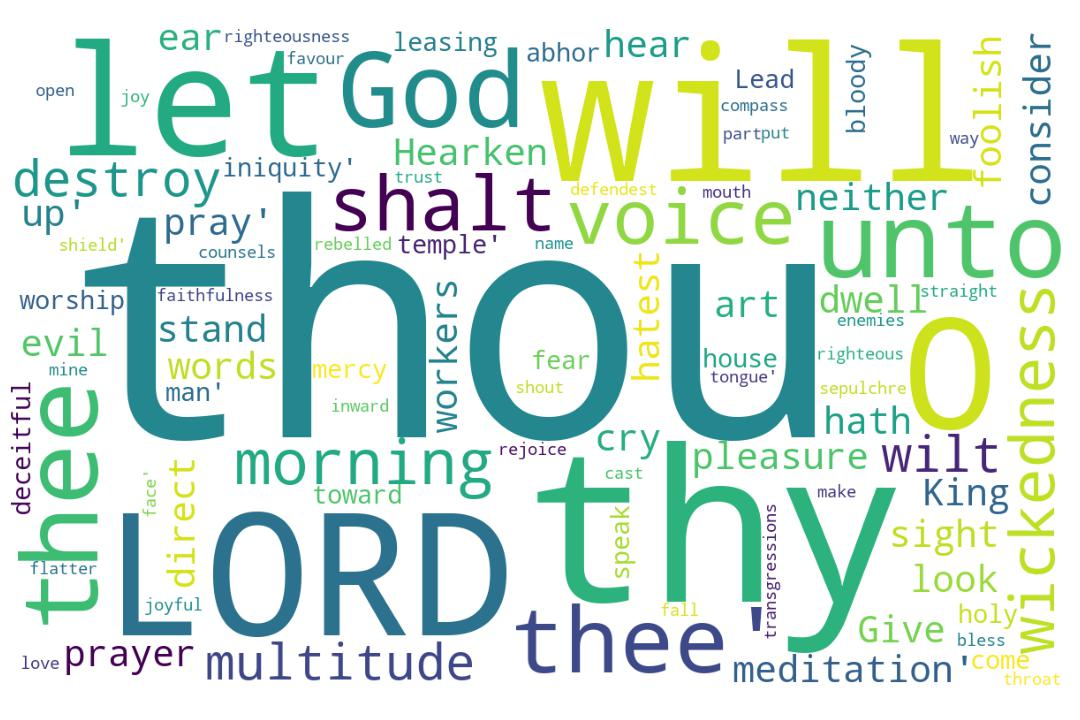
\includegraphics[width=\linewidth]{19OT-Psalms/Psalm5-WordCloud.jpg}
  \caption{Psalm 5 Word Cloud}
  \label{fig:Psalm 5 word Cloud}
\end{figure}

\marginpar{\scriptsize \centering \fcolorbox{bone}{lime}{\textbf{MEET GOD IN THE MORNING}}\\ (Psalm 5:1-12) 
\begin{compactenum}[I.][8]
    \item God has prayers \textbf{Directed} to Him \index[scripture]{Psalms!Psa 005:03}(Psa 5:3) 
    \item God \textbf{Dwells} away from Evil \index[scripture]{Psalms!Psa 005:04}(Psa 5:4)
    \item God \textbf{Detests} the Wicked \index[scripture]{Psalms!Psa 005:05}(Psa 5:5)
    \item God \textbf{Destroys} His Enemies (Psalm 5:6, 10)\index[scripture]{Psalms!Psa 005:06, 10}) 
    \item God \textbf{Describes} Rebellion \index[scripture]{Psalms!Psa 005:09}(Psa 5:9) 
    \item God \textbf{Defends} the Faithful \index[scripture]{Psalms!Psa 005:11}(Psa 5:11)
    \item God \textbf{Dispenses} Blessings \index[scripture]{Psalms!Psa 005:12}(Psa 5:12)
\end{compactenum} } 

\marginpar{\scriptsize \centering \fcolorbox{bone}{yellow}{\textbf{THOSE WHO CAN'T GO IN}}\\ (Psalm 5:1-12) 
\begin{compactenum}[I.][8]
    \item The \textbf{Foolish}  \index[scripture]{Psalms!Psa 005:5}(Psa 5:5) 
    \item The \textbf{Filthy}  \index[scripture]{Psalms!Psa 005:5}(Psa 5:5) 
    \item The \textbf{Unfearful}  \index[scripture]{Psalms!Psa 005:7}(Psa 5:7) 
    \item The \textbf{Flattering}  \index[scripture]{Psalms!Psa 005:9}(Psa 5:9) 
    \item The \textbf{Faithless}  \index[scripture]{Psalms!Psa 005:5}(Psa 5:5) 
    \item The \textbf{Unfavoured}  \index[scripture]{Psalms!Psa 005:12}(Psa 5:12) 
\end{compactenum} } 

\footnote{\textcolor[cmyk]{0.99998,1,0,0}{\hyperlink{TOC}{Return to end of Table of Contents.}}}\footnote{\href{https://audiobible.com/bible/bible.html}{\textcolor[cmyk]{0.99998,1,0,0}{Psalms Audio}}}\textcolor[cmyk]{0.99998,1,0,0}{Give\textcolor{jungle}{$_{641}$} ear to my words, O LORD, consider my meditation.}
[2] \textcolor[cmyk]{0.99998,1,0,0}{Hearken\textcolor{jungle}{$_{651}$} unto the voice of my cry, my King, and my God: for unto thee will I pray.}
[3] \textcolor[cmyk]{0.99998,1,0,0}{My\textcolor{jungle}{$_{669}$} voice shalt thou hear in the morning, O LORD; in the morning will I \fcolorbox{bone}{lime}{direct} \emph{my} \emph{prayer} unto thee, and will look up.}
[4] \textcolor[cmyk]{0.99998,1,0,0}{For\textcolor{jungle}{$_{693}$} thou \emph{art} not a God that hath pleasure in wickedness: neither shall evil \fcolorbox{bone}{lime}{dwell} with thee.}
[5] \textcolor[cmyk]{0.99998,1,0,0}{The\textcolor{jungle}{$_{710}$} foolish shall not stand in thy sight: thou \fcolorbox{bone}{lime}{hatest} all workers of iniquity.}
[6] \textcolor[cmyk]{0.99998,1,0,0}{Thou\textcolor{jungle}{$_{724}$} shalt \fcolorbox{bone}{lime}{destroy} them that speak leasing: the LORD will abhor the bloody and deceitful man.}
[7] \textcolor[cmyk]{0.99998,1,0,0}{But\textcolor{jungle}{$_{740}$} as for me, I will come \emph{into} thy house in the multitude of thy mercy: \emph{and} in thy fear will I worship toward thy holy temple.}
[8] \textcolor[cmyk]{0.99998,1,0,0}{Lead\textcolor{jungle}{$_{767}$} me, O LORD, in thy \fcolorbox{bone}{MYGOLD}{righteousness} because of mine enemies; make thy way straight before my face.}
[9] \textcolor[cmyk]{0.99998,1,0,0}{For\textcolor{jungle}{$_{785}$} \emph{there} \emph{is} no faithfulness in their mouth; their inward part \emph{is} very \fcolorbox{bone}{lime}{wickedness}; their throat \emph{is} an open \fcolorbox{bone}{lime}{sepulchre}; they flatter with their tongue.}
[10] \textcolor[cmyk]{0.99998,1,0,0}{\fcolorbox{bone}{lime}{Destroy\textcolor{jungle}{$_{810}$}} thou them, O God; let them fall by their own counsels; cast them out in the multitude of their transgressions; for they have rebelled against thee.}
[11] \textcolor[cmyk]{0.99998,1,0,0}{But\textcolor{jungle}{$_{837}$} let all those that put their trust in thee rejoice: let them ever shout for joy, because thou \fcolorbox{bone}{lime}{defendest} them: let them also that love thy name be joyful in thee.}
[12] \textcolor[cmyk]{0.99998,1,0,0}{For\textcolor{jungle}{$_{869}$} thou, LORD, wilt \fcolorbox{bone}{lime}{bless} the righteous; with favour wilt thou compass him as \emph{with} a shield\textcolor{jungle}{$_{885}$}.}




\section{Psalm 5 Comments}




%\index[NWIV]{10!Psalms!Psa 5:1}\index[AWIP]{Give!Psalms!Psa 5:1}\index[AWIP]{ear!Psalms!Psa 5:1}\index[AWIP]{to!Psalms!Psa 5:1}\index[AWIP]{my!Psalms!Psa 5:1}\index[AWIP]{my!Psalms!Psa 5:1 (2)}\index[AWIP]{words!Psalms!Psa 5:1}\index[AWIP]{O!Psalms!Psa 5:1}\index[AWIP]{LORD!Psalms!Psa 5:1}\index[AWIP]{consider!Psalms!Psa 5:1}\index[AWIP]{meditation!Psalms!Psa 5:1}

\index[NWIV]{18!Psalms!Psa 5:2}\index[AWIP]{Hearken!Psalms!Psa 5:2}\index[AWIP]{unto!Psalms!Psa 5:2}\index[AWIP]{unto!Psalms!Psa 5:2 (2)}\index[AWIP]{the!Psalms!Psa 5:2}\index[AWIP]{voice!Psalms!Psa 5:2}\index[AWIP]{of!Psalms!Psa 5:2}\index[AWIP]{my!Psalms!Psa 5:2}\index[AWIP]{my!Psalms!Psa 5:2 (2)}\index[AWIP]{my!Psalms!Psa 5:2 (3)}\index[AWIP]{cry!Psalms!Psa 5:2}\index[AWIP]{King!Psalms!Psa 5:2}\index[AWIP]{and!Psalms!Psa 5:2}\index[AWIP]{God!Psalms!Psa 5:2}\index[AWIP]{for!Psalms!Psa 5:2}\index[AWIP]{thee!Psalms!Psa 5:2}\index[AWIP]{will!Psalms!Psa 5:2}\index[AWIP]{I!Psalms!Psa 5:2}\index[AWIP]{pray!Psalms!Psa 5:2}

\index[NWIV]{24!Psalms!Psa 5:3}\index[AWIP]{My!Psalms!Psa 5:3}\index[AWIP]{voice!Psalms!Psa 5:3}\index[AWIP]{shalt!Psalms!Psa 5:3}\index[AWIP]{thou!Psalms!Psa 5:3}\index[AWIP]{hear!Psalms!Psa 5:3}\index[AWIP]{in!Psalms!Psa 5:3}\index[AWIP]{in!Psalms!Psa 5:3 (2)}\index[AWIP]{the!Psalms!Psa 5:3}\index[AWIP]{the!Psalms!Psa 5:3 (2)}\index[AWIP]{morning!Psalms!Psa 5:3}\index[AWIP]{morning!Psalms!Psa 5:3 (2)}\index[AWIP]{O!Psalms!Psa 5:3}\index[AWIP]{LORD!Psalms!Psa 5:3}\index[AWIP]{will!Psalms!Psa 5:3}\index[AWIP]{will!Psalms!Psa 5:3 (2)}\index[AWIP]{I!Psalms!Psa 5:3}\index[AWIP]{direct!Psalms!Psa 5:3}\index[AWIP]{\emph{my}!Psalms!Psa 5:3}\index[AWIP]{\emph{prayer}!Psalms!Psa 5:3}\index[AWIP]{unto!Psalms!Psa 5:3}\index[AWIP]{thee!Psalms!Psa 5:3}\index[AWIP]{and!Psalms!Psa 5:3}\index[AWIP]{look!Psalms!Psa 5:3}\index[AWIP]{up!Psalms!Psa 5:3}\index[AWIP]{\emph{my}!Psalms!Psa 5:3}\index[AWIP]{\emph{prayer}!Psalms!Psa 5:3}

\index[NWIV]{17!Psalms!Psa 5:4}\index[AWIP]{For!Psalms!Psa 5:4}\index[AWIP]{thou!Psalms!Psa 5:4}\index[AWIP]{\emph{art}!Psalms!Psa 5:4}\index[AWIP]{not!Psalms!Psa 5:4}\index[AWIP]{a!Psalms!Psa 5:4}\index[AWIP]{God!Psalms!Psa 5:4}\index[AWIP]{that!Psalms!Psa 5:4}\index[AWIP]{hath!Psalms!Psa 5:4}\index[AWIP]{pleasure!Psalms!Psa 5:4}\index[AWIP]{in!Psalms!Psa 5:4}\index[AWIP]{wickedness!Psalms!Psa 5:4}\index[AWIP]{neither!Psalms!Psa 5:4}\index[AWIP]{shall!Psalms!Psa 5:4}\index[AWIP]{evil!Psalms!Psa 5:4}\index[AWIP]{dwell!Psalms!Psa 5:4}\index[AWIP]{with!Psalms!Psa 5:4}\index[AWIP]{thee!Psalms!Psa 5:4}\index[AWIP]{\emph{art}!Psalms!Psa 5:4}

\index[NWIV]{14!Psalms!Psa 5:5}\index[AWIP]{The!Psalms!Psa 5:5}\index[AWIP]{foolish!Psalms!Psa 5:5}\index[AWIP]{shall!Psalms!Psa 5:5}\index[AWIP]{not!Psalms!Psa 5:5}\index[AWIP]{stand!Psalms!Psa 5:5}\index[AWIP]{in!Psalms!Psa 5:5}\index[AWIP]{thy!Psalms!Psa 5:5}\index[AWIP]{sight!Psalms!Psa 5:5}\index[AWIP]{thou!Psalms!Psa 5:5}\index[AWIP]{hatest!Psalms!Psa 5:5}\index[AWIP]{all!Psalms!Psa 5:5}\index[AWIP]{workers!Psalms!Psa 5:5}\index[AWIP]{of!Psalms!Psa 5:5}\index[AWIP]{iniquity!Psalms!Psa 5:5}

\index[NWIV]{16!Psalms!Psa 5:6}\index[AWIP]{Thou!Psalms!Psa 5:6}\index[AWIP]{shalt!Psalms!Psa 5:6}\index[AWIP]{destroy!Psalms!Psa 5:6}\index[AWIP]{them!Psalms!Psa 5:6}\index[AWIP]{that!Psalms!Psa 5:6}\index[AWIP]{speak!Psalms!Psa 5:6}\index[AWIP]{leasing!Psalms!Psa 5:6}\index[AWIP]{the!Psalms!Psa 5:6}\index[AWIP]{the!Psalms!Psa 5:6 (2)}\index[AWIP]{LORD!Psalms!Psa 5:6}\index[AWIP]{will!Psalms!Psa 5:6}\index[AWIP]{abhor!Psalms!Psa 5:6}\index[AWIP]{bloody!Psalms!Psa 5:6}\index[AWIP]{and!Psalms!Psa 5:6}\index[AWIP]{deceitful!Psalms!Psa 5:6}\index[AWIP]{man!Psalms!Psa 5:6}

\index[NWIV]{27!Psalms!Psa 5:7}\index[AWIP]{But!Psalms!Psa 5:7}\index[AWIP]{as!Psalms!Psa 5:7}\index[AWIP]{for!Psalms!Psa 5:7}\index[AWIP]{me!Psalms!Psa 5:7}\index[AWIP]{I!Psalms!Psa 5:7}\index[AWIP]{I!Psalms!Psa 5:7 (2)}\index[AWIP]{will!Psalms!Psa 5:7}\index[AWIP]{will!Psalms!Psa 5:7 (2)}\index[AWIP]{come!Psalms!Psa 5:7}\index[AWIP]{\emph{into}!Psalms!Psa 5:7}\index[AWIP]{thy!Psalms!Psa 5:7}\index[AWIP]{thy!Psalms!Psa 5:7 (2)}\index[AWIP]{thy!Psalms!Psa 5:7 (3)}\index[AWIP]{thy!Psalms!Psa 5:7 (4)}\index[AWIP]{house!Psalms!Psa 5:7}\index[AWIP]{in!Psalms!Psa 5:7}\index[AWIP]{in!Psalms!Psa 5:7 (2)}\index[AWIP]{the!Psalms!Psa 5:7}\index[AWIP]{multitude!Psalms!Psa 5:7}\index[AWIP]{of!Psalms!Psa 5:7}\index[AWIP]{mercy!Psalms!Psa 5:7}\index[AWIP]{\emph{and}!Psalms!Psa 5:7}\index[AWIP]{fear!Psalms!Psa 5:7}\index[AWIP]{worship!Psalms!Psa 5:7}\index[AWIP]{toward!Psalms!Psa 5:7}\index[AWIP]{holy!Psalms!Psa 5:7}\index[AWIP]{temple!Psalms!Psa 5:7}\index[AWIP]{\emph{into}!Psalms!Psa 5:7}\index[AWIP]{\emph{and}!Psalms!Psa 5:7}

\index[NWIV]{18!Psalms!Psa 5:8}\index[AWIP]{Lead!Psalms!Psa 5:8}\index[AWIP]{me!Psalms!Psa 5:8}\index[AWIP]{O!Psalms!Psa 5:8}\index[AWIP]{LORD!Psalms!Psa 5:8}\index[AWIP]{in!Psalms!Psa 5:8}\index[AWIP]{thy!Psalms!Psa 5:8}\index[AWIP]{thy!Psalms!Psa 5:8 (2)}\index[AWIP]{righteousness!Psalms!Psa 5:8}\index[AWIP]{because!Psalms!Psa 5:8}\index[AWIP]{of!Psalms!Psa 5:8}\index[AWIP]{mine!Psalms!Psa 5:8}\index[AWIP]{enemies!Psalms!Psa 5:8}\index[AWIP]{make!Psalms!Psa 5:8}\index[AWIP]{way!Psalms!Psa 5:8}\index[AWIP]{straight!Psalms!Psa 5:8}\index[AWIP]{before!Psalms!Psa 5:8}\index[AWIP]{my!Psalms!Psa 5:8}\index[AWIP]{face!Psalms!Psa 5:8}

\index[NWIV]{25!Psalms!Psa 5:9}\index[AWIP]{For!Psalms!Psa 5:9}\index[AWIP]{\emph{there}!Psalms!Psa 5:9}\index[AWIP]{\emph{is}!Psalms!Psa 5:9}\index[AWIP]{\emph{is}!Psalms!Psa 5:9 (2)}\index[AWIP]{\emph{is}!Psalms!Psa 5:9 (3)}\index[AWIP]{no!Psalms!Psa 5:9}\index[AWIP]{faithfulness!Psalms!Psa 5:9}\index[AWIP]{in!Psalms!Psa 5:9}\index[AWIP]{their!Psalms!Psa 5:9}\index[AWIP]{their!Psalms!Psa 5:9 (2)}\index[AWIP]{their!Psalms!Psa 5:9 (3)}\index[AWIP]{their!Psalms!Psa 5:9 (4)}\index[AWIP]{mouth!Psalms!Psa 5:9}\index[AWIP]{inward!Psalms!Psa 5:9}\index[AWIP]{part!Psalms!Psa 5:9}\index[AWIP]{very!Psalms!Psa 5:9}\index[AWIP]{wickedness!Psalms!Psa 5:9}\index[AWIP]{throat!Psalms!Psa 5:9}\index[AWIP]{an!Psalms!Psa 5:9}\index[AWIP]{open!Psalms!Psa 5:9}\index[AWIP]{sepulchre!Psalms!Psa 5:9}\index[AWIP]{they!Psalms!Psa 5:9}\index[AWIP]{flatter!Psalms!Psa 5:9}\index[AWIP]{with!Psalms!Psa 5:9}\index[AWIP]{tongue!Psalms!Psa 5:9}\index[AWIP]{\emph{there}!Psalms!Psa 5:9}\index[AWIP]{\emph{is}!Psalms!Psa 5:9}\index[AWIP]{\emph{is}!Psalms!Psa 5:9 (2)}\index[AWIP]{\emph{is}!Psalms!Psa 5:9 (3)}

\index[NWIV]{27!Psalms!Psa 5:10}\index[AWIP]{Destroy!Psalms!Psa 5:10}\index[AWIP]{thou!Psalms!Psa 5:10}\index[AWIP]{them!Psalms!Psa 5:10}\index[AWIP]{them!Psalms!Psa 5:10 (2)}\index[AWIP]{them!Psalms!Psa 5:10 (3)}\index[AWIP]{O!Psalms!Psa 5:10}\index[AWIP]{God!Psalms!Psa 5:10}\index[AWIP]{let!Psalms!Psa 5:10}\index[AWIP]{fall!Psalms!Psa 5:10}\index[AWIP]{by!Psalms!Psa 5:10}\index[AWIP]{their!Psalms!Psa 5:10}\index[AWIP]{their!Psalms!Psa 5:10 (2)}\index[AWIP]{own!Psalms!Psa 5:10}\index[AWIP]{counsels!Psalms!Psa 5:10}\index[AWIP]{cast!Psalms!Psa 5:10}\index[AWIP]{out!Psalms!Psa 5:10}\index[AWIP]{in!Psalms!Psa 5:10}\index[AWIP]{the!Psalms!Psa 5:10}\index[AWIP]{multitude!Psalms!Psa 5:10}\index[AWIP]{of!Psalms!Psa 5:10}\index[AWIP]{transgressions!Psalms!Psa 5:10}\index[AWIP]{for!Psalms!Psa 5:10}\index[AWIP]{they!Psalms!Psa 5:10}\index[AWIP]{have!Psalms!Psa 5:10}\index[AWIP]{rebelled!Psalms!Psa 5:10}\index[AWIP]{against!Psalms!Psa 5:10}\index[AWIP]{thee!Psalms!Psa 5:10}

\index[NWIV]{32!Psalms!Psa 5:11}\index[AWIP]{But!Psalms!Psa 5:11}\index[AWIP]{let!Psalms!Psa 5:11}\index[AWIP]{let!Psalms!Psa 5:11 (2)}\index[AWIP]{let!Psalms!Psa 5:11 (3)}\index[AWIP]{all!Psalms!Psa 5:11}\index[AWIP]{those!Psalms!Psa 5:11}\index[AWIP]{that!Psalms!Psa 5:11}\index[AWIP]{that!Psalms!Psa 5:11 (2)}\index[AWIP]{put!Psalms!Psa 5:11}\index[AWIP]{their!Psalms!Psa 5:11}\index[AWIP]{trust!Psalms!Psa 5:11}\index[AWIP]{in!Psalms!Psa 5:11}\index[AWIP]{in!Psalms!Psa 5:11 (2)}\index[AWIP]{thee!Psalms!Psa 5:11}\index[AWIP]{thee!Psalms!Psa 5:11 (2)}\index[AWIP]{rejoice!Psalms!Psa 5:11}\index[AWIP]{them!Psalms!Psa 5:11}\index[AWIP]{them!Psalms!Psa 5:11 (2)}\index[AWIP]{them!Psalms!Psa 5:11 (3)}\index[AWIP]{ever!Psalms!Psa 5:11}\index[AWIP]{shout!Psalms!Psa 5:11}\index[AWIP]{for!Psalms!Psa 5:11}\index[AWIP]{joy!Psalms!Psa 5:11}\index[AWIP]{because!Psalms!Psa 5:11}\index[AWIP]{thou!Psalms!Psa 5:11}\index[AWIP]{defendest!Psalms!Psa 5:11}\index[AWIP]{also!Psalms!Psa 5:11}\index[AWIP]{love!Psalms!Psa 5:11}\index[AWIP]{thy!Psalms!Psa 5:11}\index[AWIP]{name!Psalms!Psa 5:11}\index[AWIP]{be!Psalms!Psa 5:11}\index[AWIP]{joyful!Psalms!Psa 5:11}

\index[NWIV]{17!Psalms!Psa 5:12}\index[AWIP]{For!Psalms!Psa 5:12}\index[AWIP]{thou!Psalms!Psa 5:12}\index[AWIP]{thou!Psalms!Psa 5:12 (2)}\index[AWIP]{LORD!Psalms!Psa 5:12}\index[AWIP]{wilt!Psalms!Psa 5:12}\index[AWIP]{wilt!Psalms!Psa 5:12 (2)}\index[AWIP]{bless!Psalms!Psa 5:12}\index[AWIP]{the!Psalms!Psa 5:12}\index[AWIP]{righteous!Psalms!Psa 5:12}\index[AWIP]{with!Psalms!Psa 5:12}\index[AWIP]{favour!Psalms!Psa 5:12}\index[AWIP]{compass!Psalms!Psa 5:12}\index[AWIP]{him!Psalms!Psa 5:12}\index[AWIP]{as!Psalms!Psa 5:12}\index[AWIP]{\emph{with}!Psalms!Psa 5:12}\index[AWIP]{a!Psalms!Psa 5:12}\index[AWIP]{shield!Psalms!Psa 5:12}\index[AWIP]{\emph{with}!Psalms!Psa 5:12}


\section{Psalm 5 Outlines}

\subsection{My Outlines}

\subsubsection{Meet God in the Morning}
%\textbf{Introduction:} Psalm 5:\footnote{11 June 2016, Keith Anthony}
\index[speaker]{Keith Anthony!Psalm 005 (Meet God in the Morning)}
\index[series]{Psalms (Keith Anthony)!Psalm 005 (Meet God in the Morning)}
\index[date]{2016/06/11!Psalm 005 (Meet God in the Morning)}
\begin{compactenum}[I.]
    \item God has prayers \textbf{Directed} to Him \index[scripture]{Psalms!Psa 005:03}(Psa 5:3) 
    \item God \textbf{Dwells} away from Evil \index[scripture]{Psalms!Psa 005:04}(Psa 5:4)
    \item God \textbf{Detests} the Wicked \index[scripture]{Psalms!Psa 005:05}(Psa 5:5)
    \item God \textbf{Destroys} His Enemies (Psalm 5:6, 10)\index[scripture]{Psalms!Psa 005:06, 10}) 
    \item God \textbf{Describes} Rebellion \index[scripture]{Psalms!Psa 005:09}(Psa 5:9) 
    \item God \textbf{Defends} the Faithful \index[scripture]{Psalms!Psa 005:11}(Psa 5:11)
    \item God \textbf{Dispenses} Blessings \index[scripture]{Psalms!Psa 005:12}(Psa 5:12)
\end{compactenum}



\subsubsection{Those Who Can't Go In}
%\textbf{Introduction:} Psalm 5:\footnote{11 June 2016, Keith Anthony}
\index[speaker]{Keith Anthony!Psalm 005 (Those Who Can't Go In)}
\index[series]{Psalms (Keith Anthony)!Psalm 005 (Those Who Can't Go In)}
\index[date]{2020/06/25!Psalm 005 (Those Who Can't Go In)}

\begin{compactenum}[I.][8]
    \item The \textbf{Foolish}  \index[scripture]{Psalms!Psa 005:5}(Psa 5:5) 
    \item The \textbf{Filthy}  \index[scripture]{Psalms!Psa 005:5}(Psa 5:5) 
    \item The \textbf{Unfearful}  \index[scripture]{Psalms!Psa 005:7}(Psa 5:7) 
    \item The \textbf{Flattering}  \index[scripture]{Psalms!Psa 005:9}(Psa 5:9) 
    \item The \textbf{Faithless}  \index[scripture]{Psalms!Psa 005:5}(Psa 5:5) 
    \item The \textbf{Unfavoured}  \index[scripture]{Psalms!Psa 005:12}(Psa 5:12) 
\end{compactenum} 


\subsection{Outlines from Others}


%\section{Psalm 5 Statistics}

%%%%%%%%%%%%%%%%%%%%%%%%%%%
%%%%%Word Statistics
%%%%%%%%%%%%%%%%%%%%%%%%%%%


\normalsize



\subsection{Chapter Word Statistics}


%%%%%%%%%%
%%%%%%%%%%
 
\begin{center}
\begin{longtable}{l|c|c|c|c}
\caption[Stats for Psalm 5]{Stats for Psalm 5} \label{table:Stats for Psalm 5} \\ 
\hline \multicolumn{1}{|c|}{\textbf{Verse(s)}} & \multicolumn{1}{|c|}{\textbf{Count}} & \multicolumn{1}{|c|}{\textbf{Unique}} & \multicolumn{1}{|c|}{\textbf{Italics}} & \multicolumn{1}{|c|}{\textbf{Uniq Italic}}  \\ \hline 
\endfirsthead
 
\multicolumn{5}{c}
{{\bfseries \tablename\ \thetable{} -- continued from previous page}} \\  
\hline \multicolumn{1}{|c|}{\textbf{Verse(s)}} & \multicolumn{1}{|c|}{\textbf{Count}} & \multicolumn{1}{|c|}{\textbf{Unique}} & \multicolumn{1}{|c|}{\textbf{Italics}} & \multicolumn{1}{|c|}{\textbf{Uniq Italic}}  \\ \hline 
\endhead
 
\hline \multicolumn{5}{|r|}{{Continued if needed}} \\ \hline
\endfoot 
1 & 10 & 9 & 0 & 0\\ \hline
2 & 18 & 15 & 0 & 0\\ \hline
3 & 24 & 20 & 2 & 2\\ \hline
4 & 17 & 17 & 1 & 1\\ \hline
5 & 14 & 14 & 0 & 0\\ \hline
6 & 16 & 15 & 0 & 0\\ \hline
7 & 27 & 21 & 2 & 2\\ \hline
8 & 18 & 17 & 0 & 0\\ \hline
9 & 25 & 20 & 4 & 2\\ \hline
10 & 27 & 24 & 0 & 0\\ \hline
11 & 32 & 25 & 0 & 0\\ \hline
12 & 17 & 15 & 1 & 1\\ \hline
\hline \hline
Total & 245 & 138 & 10 & 8



\end{longtable}
\end{center}

%%%%%%%%%%
%%%%%%%%%%
 
\subsection{Words by Frequency}

\begin{center}
\begin{longtable}{l|r}
\caption[Word Frequencies in Psalm 5]{Word Frequencies in Psalm 5} \label{table:WordsIn-Psalm-5} \\ 
\hline \multicolumn{1}{|c|}{\textbf{Word}} & \multicolumn{1}{c|}{\textbf{Frequency}} \\ \hline 
\endfirsthead
 
\multicolumn{2}{c}
{{\bfseries \tablename\ \thetable{} -- continued from previous page}} \\ 
\hline \multicolumn{1}{|c|}{\textbf{Word}} & \multicolumn{1}{c|}{\textbf{Frequency}} \\ \hline 
\endhead
 
\hline \multicolumn{2}{|r|}{{Continued if needed}} \\ \hline
\endfoot
 
\hline \hline
\endlastfoot
in & 11 \\ \hline
the & 8 \\ \hline
thy & 8 \\ \hline
thou & 7 \\ \hline
them & 7 \\ \hline
their & 7 \\ \hline
my & 6 \\ \hline
thee & 6 \\ \hline
will & 6 \\ \hline
LORD & 5 \\ \hline
of & 5 \\ \hline
O & 4 \\ \hline
for & 4 \\ \hline
I & 4 \\ \hline
that & 4 \\ \hline
let & 4 \\ \hline
unto & 3 \\ \hline
and & 3 \\ \hline
God & 3 \\ \hline
For & 3 \\ \hline
with & 3 \\ \hline
\emph{is} & 3 \\ \hline
voice & 2 \\ \hline
shalt & 2 \\ \hline
morning & 2 \\ \hline
not & 2 \\ \hline
a & 2 \\ \hline
wickedness & 2 \\ \hline
shall & 2 \\ \hline
all & 2 \\ \hline
But & 2 \\ \hline
as & 2 \\ \hline
me & 2 \\ \hline
multitude & 2 \\ \hline
because & 2 \\ \hline
they & 2 \\ \hline
wilt & 2 \\ \hline
Give & 1 \\ \hline
ear & 1 \\ \hline
to & 1 \\ \hline
words & 1 \\ \hline
consider & 1 \\ \hline
meditation & 1 \\ \hline
Hearken & 1 \\ \hline
cry & 1 \\ \hline
King & 1 \\ \hline
pray & 1 \\ \hline
My & 1 \\ \hline
hear & 1 \\ \hline
direct & 1 \\ \hline
\emph{my} & 1 \\ \hline
\emph{prayer} & 1 \\ \hline
look & 1 \\ \hline
up & 1 \\ \hline
\emph{art} & 1 \\ \hline
hath & 1 \\ \hline
pleasure & 1 \\ \hline
neither & 1 \\ \hline
evil & 1 \\ \hline
dwell & 1 \\ \hline
The & 1 \\ \hline
foolish & 1 \\ \hline
stand & 1 \\ \hline
sight & 1 \\ \hline
hatest & 1 \\ \hline
workers & 1 \\ \hline
iniquity & 1 \\ \hline
Thou & 1 \\ \hline
destroy & 1 \\ \hline
speak & 1 \\ \hline
leasing & 1 \\ \hline
abhor & 1 \\ \hline
bloody & 1 \\ \hline
deceitful & 1 \\ \hline
man & 1 \\ \hline
come & 1 \\ \hline
\emph{into} & 1 \\ \hline
house & 1 \\ \hline
mercy & 1 \\ \hline
\emph{and} & 1 \\ \hline
fear & 1 \\ \hline
worship & 1 \\ \hline
toward & 1 \\ \hline
holy & 1 \\ \hline
temple & 1 \\ \hline
Lead & 1 \\ \hline
righteousness & 1 \\ \hline
mine & 1 \\ \hline
enemies & 1 \\ \hline
make & 1 \\ \hline
way & 1 \\ \hline
straight & 1 \\ \hline
before & 1 \\ \hline
face & 1 \\ \hline
\emph{there} & 1 \\ \hline
no & 1 \\ \hline
faithfulness & 1 \\ \hline
mouth & 1 \\ \hline
inward & 1 \\ \hline
part & 1 \\ \hline
very & 1 \\ \hline
throat & 1 \\ \hline
an & 1 \\ \hline
open & 1 \\ \hline
sepulchre & 1 \\ \hline
flatter & 1 \\ \hline
tongue & 1 \\ \hline
Destroy & 1 \\ \hline
fall & 1 \\ \hline
by & 1 \\ \hline
own & 1 \\ \hline
counsels & 1 \\ \hline
cast & 1 \\ \hline
out & 1 \\ \hline
transgressions & 1 \\ \hline
have & 1 \\ \hline
rebelled & 1 \\ \hline
against & 1 \\ \hline
those & 1 \\ \hline
put & 1 \\ \hline
trust & 1 \\ \hline
rejoice & 1 \\ \hline
ever & 1 \\ \hline
shout & 1 \\ \hline
joy & 1 \\ \hline
defendest & 1 \\ \hline
also & 1 \\ \hline
love & 1 \\ \hline
name & 1 \\ \hline
be & 1 \\ \hline
joyful & 1 \\ \hline
bless & 1 \\ \hline
righteous & 1 \\ \hline
favour & 1 \\ \hline
compass & 1 \\ \hline
him & 1 \\ \hline
\emph{with} & 1 \\ \hline
shield & 1 \\ \hline
\end{longtable}
\end{center}



\normalsize



\subsection{Words Alphabetically}

\begin{center}
\begin{longtable}{l|r}
\caption[Word Alphabetically in Psalm 5]{Word Alphabetically in Psalm 5} \label{table:WordsIn-Psalm-5} \\ 
\hline \multicolumn{1}{|c|}{\textbf{Word}} & \multicolumn{1}{c|}{\textbf{Frequency}} \\ \hline 
\endfirsthead
 
\multicolumn{2}{c}
{{\bfseries \tablename\ \thetable{} -- continued from previous page}} \\ 
\hline \multicolumn{1}{|c|}{\textbf{Word}} & \multicolumn{1}{c|}{\textbf{Frequency}} \\ \hline 
\endhead
 
\hline \multicolumn{2}{|r|}{{Continued if needed}} \\ \hline
\endfoot
 
\hline \hline
\endlastfoot
But & 2 \\ \hline
Destroy & 1 \\ \hline
For & 3 \\ \hline
Give & 1 \\ \hline
God & 3 \\ \hline
Hearken & 1 \\ \hline
I & 4 \\ \hline
King & 1 \\ \hline
LORD & 5 \\ \hline
Lead & 1 \\ \hline
My & 1 \\ \hline
O & 4 \\ \hline
The & 1 \\ \hline
Thou & 1 \\ \hline
\emph{and} & 1 \\ \hline
\emph{art} & 1 \\ \hline
\emph{into} & 1 \\ \hline
\emph{is} & 3 \\ \hline
\emph{my} & 1 \\ \hline
\emph{prayer} & 1 \\ \hline
\emph{there} & 1 \\ \hline
\emph{with} & 1 \\ \hline
a & 2 \\ \hline
abhor & 1 \\ \hline
against & 1 \\ \hline
all & 2 \\ \hline
also & 1 \\ \hline
an & 1 \\ \hline
and & 3 \\ \hline
as & 2 \\ \hline
be & 1 \\ \hline
because & 2 \\ \hline
before & 1 \\ \hline
bless & 1 \\ \hline
bloody & 1 \\ \hline
by & 1 \\ \hline
cast & 1 \\ \hline
come & 1 \\ \hline
compass & 1 \\ \hline
consider & 1 \\ \hline
counsels & 1 \\ \hline
cry & 1 \\ \hline
deceitful & 1 \\ \hline
defendest & 1 \\ \hline
destroy & 1 \\ \hline
direct & 1 \\ \hline
dwell & 1 \\ \hline
ear & 1 \\ \hline
enemies & 1 \\ \hline
ever & 1 \\ \hline
evil & 1 \\ \hline
face & 1 \\ \hline
faithfulness & 1 \\ \hline
fall & 1 \\ \hline
favour & 1 \\ \hline
fear & 1 \\ \hline
flatter & 1 \\ \hline
foolish & 1 \\ \hline
for & 4 \\ \hline
hatest & 1 \\ \hline
hath & 1 \\ \hline
have & 1 \\ \hline
hear & 1 \\ \hline
him & 1 \\ \hline
holy & 1 \\ \hline
house & 1 \\ \hline
in & 11 \\ \hline
iniquity & 1 \\ \hline
inward & 1 \\ \hline
joy & 1 \\ \hline
joyful & 1 \\ \hline
leasing & 1 \\ \hline
let & 4 \\ \hline
look & 1 \\ \hline
love & 1 \\ \hline
make & 1 \\ \hline
man & 1 \\ \hline
me & 2 \\ \hline
meditation & 1 \\ \hline
mercy & 1 \\ \hline
mine & 1 \\ \hline
morning & 2 \\ \hline
mouth & 1 \\ \hline
multitude & 2 \\ \hline
my & 6 \\ \hline
name & 1 \\ \hline
neither & 1 \\ \hline
no & 1 \\ \hline
not & 2 \\ \hline
of & 5 \\ \hline
open & 1 \\ \hline
out & 1 \\ \hline
own & 1 \\ \hline
part & 1 \\ \hline
pleasure & 1 \\ \hline
pray & 1 \\ \hline
put & 1 \\ \hline
rebelled & 1 \\ \hline
rejoice & 1 \\ \hline
righteous & 1 \\ \hline
righteousness & 1 \\ \hline
sepulchre & 1 \\ \hline
shall & 2 \\ \hline
shalt & 2 \\ \hline
shield & 1 \\ \hline
shout & 1 \\ \hline
sight & 1 \\ \hline
speak & 1 \\ \hline
stand & 1 \\ \hline
straight & 1 \\ \hline
temple & 1 \\ \hline
that & 4 \\ \hline
the & 8 \\ \hline
thee & 6 \\ \hline
their & 7 \\ \hline
them & 7 \\ \hline
they & 2 \\ \hline
those & 1 \\ \hline
thou & 7 \\ \hline
throat & 1 \\ \hline
thy & 8 \\ \hline
to & 1 \\ \hline
tongue & 1 \\ \hline
toward & 1 \\ \hline
transgressions & 1 \\ \hline
trust & 1 \\ \hline
unto & 3 \\ \hline
up & 1 \\ \hline
very & 1 \\ \hline
voice & 2 \\ \hline
way & 1 \\ \hline
wickedness & 2 \\ \hline
will & 6 \\ \hline
wilt & 2 \\ \hline
with & 3 \\ \hline
words & 1 \\ \hline
workers & 1 \\ \hline
worship & 1 \\ \hline
\end{longtable}
\end{center}



\normalsize



\subsection{Word Lengths in Chapter}
\normalsize
\begin{longtable}{l|p{3.75in}}
\caption[Words by Length in Psalm 5]{Words by Length in Psalm 5} \label{table:WordsIn-Psalm-5} \\ 
\hline \multicolumn{1}{|c|}{\textbf{Length}} & \multicolumn{1}{c|}{\textbf{Words}} \\ \hline 
\endfirsthead
 
\multicolumn{2}{c}
{{\bfseries \tablename\ \thetable{} -- continued from previous page}} \\ 
\hline \multicolumn{1}{|c|}{\textbf{Length}} & \multicolumn{1}{c|}{\textbf{Words}} \\ \hline 
\endhead
 
\hline \multicolumn{2}{|r|}{{Continued if needed}} \\ \hline
\endfoot
 
\hline \hline
\endlastfoot
1 & O, I, a \\ \hline
2 & to, my, of, My, in, \emph{my}, up, as, me, \emph{is}, no, an, by, be \\ \hline
3 & ear, the, cry, and, God, for, For, \emph{art}, not, The, thy, all, man, But, \emph{and}, way, let, own, out, put, joy, him \\ \hline
4 & Give, LORD, unto, King, thee, will, pray, thou, hear, look, that, hath, evil, with, Thou, them, come, \emph{into}, fear, holy, Lead, mine, make, face, part, very, open, they, fall, cast, have, ever, also, love, name, wilt, \emph{with} \\ \hline
5 & words, voice, shalt, shall, dwell, stand, sight, speak, abhor, house, mercy, \emph{there}, their, mouth, those, trust, shout, bless \\ \hline
6 & direct, \emph{prayer}, hatest, bloody, toward, temple, before, inward, throat, tongue, joyful, favour, shield \\ \hline
7 & Hearken, morning, neither, foolish, workers, destroy, leasing, worship, because, enemies, flatter, Destroy, against, rejoice, compass \\ \hline
8 & consider, pleasure, iniquity, straight, counsels, rebelled \\ \hline
9 & deceitful, multitude, sepulchre, defendest, righteous \\ \hline
10 & meditation, wickedness \\ \hline
12 & faithfulness \\ \hline
13 & righteousness \\ \hline
14 & transgressions \\ \hline
\end{longtable}






%%%%%%%%%%
%%%%%%%%%%
 



%%%%%%%%%%
%%%%%%%%%%
\subsection{Verses with 18 Words in Chapter}
\normalsize
\begin{longtable}{l|p{3.75in}}
\caption[Verses with 18 Words  in Psalm 5]{Verses with 18 Words  in Psalm 5} \label{table:Verses with 18 Words in-Psalm-5} \\ 
\hline \multicolumn{1}{|c|}{\textbf{Reference}} & \multicolumn{1}{c|}{\textbf{Verse}} \\ \hline 
\endfirsthead
 
\multicolumn{2}{c}
{{\bfseries \tablename\ \thetable{} -- continued from previous page}} \\ 
\hline \multicolumn{1}{|c|}{\textbf{Reference}} & \multicolumn{1}{c|}{\textbf{Verse}} \\ \hline 
\endhead
 
\hline \multicolumn{2}{|r|}{{Continued if needed}} \\ \hline
\endfoot
 
\hline \hline
\endlastfoot
Psalms 005:2 & Hearken unto the voice of my cry, my King, and my God: for unto thee will I pray. \\ \hline
Psalms 005:8 & Lead me, O LORD, in thy righteousness because of mine enemies; make thy way straight before my face. \\ \hline
\end{longtable}






%%%%%%%%%%
%%%%%%%%%%
\subsection{Psalm5 Repeated Phrases}


%%%%%%%%%%
%%%%%%%%%%
\normalsize
 
\begin{center}
\begin{longtable}{|p{3.0in}|p{0.5in}|}
\caption[Psalm5 Repeated Phrases]{Psalm5 Repeated Phrases}\label{table:Repeated Phrases Psalm5} \\
\hline \multicolumn{1}{|c|}{\textbf{Phrase}} & \multicolumn{1}{c|}{\textbf{Frequency}} \\ \hline 
\endfirsthead
 
\multicolumn{2}{c}
{{\bfseries \tablename\ \thetable{} -- continued from previous page}} \\  
\hline \multicolumn{1}{|c|}{\textbf{Phrase}} & \multicolumn{1}{c|}{\textbf{Frequency}} \\ \hline 
\endhead
 
\hline \multicolumn{2}{c}{{ }} \\ \hline
\endfoot 
in the & 4\\ \hline 
O LORD & 3\\ \hline 
will I & 3\\ \hline 
in thy & 3\\ \hline 
let them & 3\\ \hline 
\end{longtable}
\end{center}



%%%%%%%%%%
%%%%%%%%%%




\chapter{Psalm 6}

\begin{figure}
  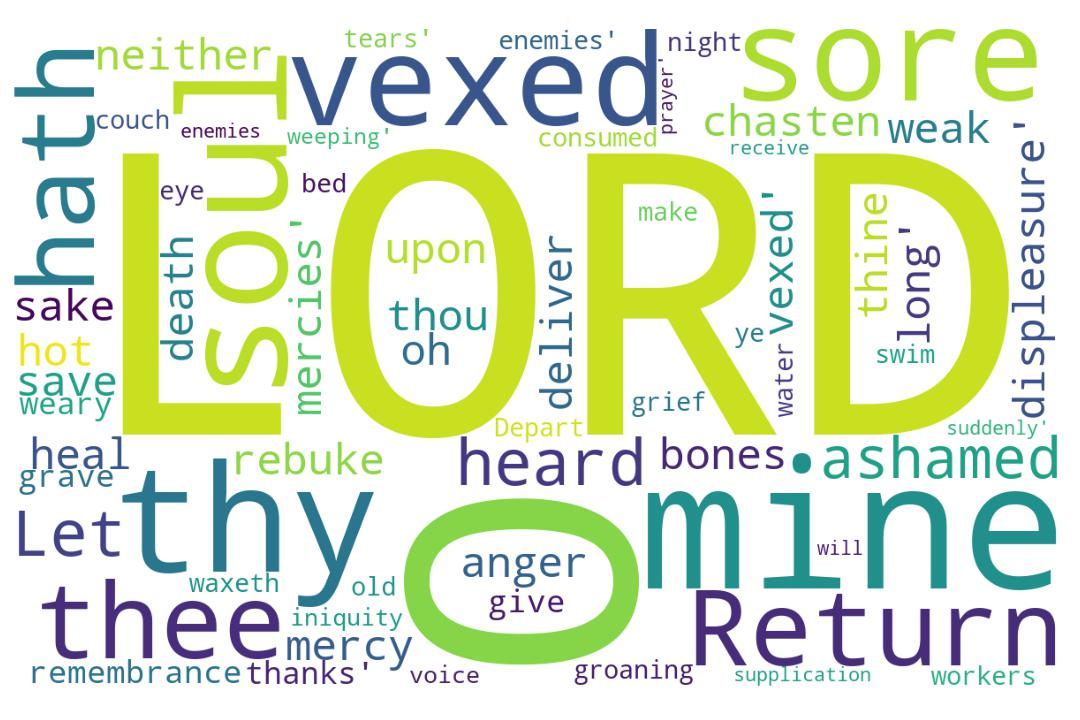
\includegraphics[width=\linewidth]{19OT-Psalms/Psalm6-WordCloud.jpg}
  \caption{Psalm 6 Word Cloud}
  \label{fig:Psalm 6 word Cloud}
\end{figure}

\marginpar{\scriptsize \centering \fcolorbox{bone}{lime}{\textbf{WHEN GOD IS NEAR}}\\ (Psalm 6:1-10) 
\begin{compactenum}[I.][8]
    \item \textbf{Recognize Sin and its Damage}  \index[scripture]{Psalms!Psa 006:02} (Psa 6:2)
    \item \textbf{Reach a State of Despair} \index[scripture]{Psalms!Psa 006:03} (Psa 6:3)
    \item \textbf{Remember the Source of his Deliverance} \index[scripture]{Psalms!Psa 006:04} (Psa 6:4)
    \item \textbf{Repeat his Sorrow and Distress} \index[scripture]{Psalms!Psa 006:06} (Psa 6:6)
    \item \textbf{Recount the Sum of Adversaries} \index[scripture]{Psalms!Psa 006:07} (Psa 6:7)
    \item \textbf{Request for Sinners to Depart} \index[scripture]{Psalms!Psa 006:08} (Psa 6:8)
    \item \textbf{Rejoice in the Savior and Deliverer} \index[scripture]{Psalms!Psa 006:09} (Psa 6:9)
\end{compactenum} } 

\marginpar{\scriptsize \centering \fcolorbox{bone}{yellow}{\textbf{THE PSALMIST'S SITUATION}}\\ (Psalm 6:1-10) 
\begin{compactenum}[I.][8]
     \item Acknowledges the \textbf{Sinner Deserves God's Anger}  \index[scripture]{Psalms!Psa 006:01} (Psa 6:1)
    \item Acknowledges the \textbf{Sinner has Earned God's Displeasure}  \index[scripture]{Psalms!Psa 006:01} (Psa 6:1)
    \item He \textbf{Is Desiring Mercy}  \index[scripture]{Psalms!Psa 006:02} (Psa 6:2)
    \item Knows God \textbf{Can Deliver Souls}  \index[scripture]{Psalms!Psa 006:04} (Psa 6:4)
    \item Knows The \textbf{Dead have no Hope}  \index[scripture]{Psalms!Psa 006:05} (Psa 6:5)
    \item Chooses to \textbf{Depart} from Sinners \index[scripture]{Psalms!Psa 006:08} (Psa 6:8)
    \item \textbf{Depends} on God's Reponses \index[scripture]{Psalms!Psa 006:09} (Psa 6:9)
\end{compactenum} } 

\footnote{\textcolor[cmyk]{0.99998,1,0,0}{\hyperlink{TOC}{Return to end of Table of Contents.}}}\footnote{\href{https://audiobible.com/bible/bible.html}{\textcolor[cmyk]{0.99998,1,0,0}{Psalms Audio}}}\textcolor[cmyk]{0.99998,1,0,0}{To the chief musician on Neginoth upon Sheminith. A Psalm of David.}\\
\\
\textcolor[cmyk]{0.99998,1,0,0}{O LORD, rebuke me not in thine anger, neither chasten me in thy hot displeasure.}
[2] \textcolor[cmyk]{0.99998,1,0,0}{Have mercy upon me, O LORD; for I \emph{am} weak: O LORD, heal me; for my bones are vexed.}
[3] \textcolor[cmyk]{0.99998,1,0,0}{My soul is also sore vexed: but thou, O LORD, how long?}
[4] \textcolor[cmyk]{0.99998,1,0,0}{Return, O LORD, deliver my soul: oh save me for thy mercies' sake.}
[5] \textcolor[cmyk]{0.99998,1,0,0}{For in death \emph{there} \emph{is} no remembrance of thee: in the grave who shall give thee thanks?}
[6] \textcolor[cmyk]{0.99998,1,0,0}{I am weary with my groaning; all the night make I my bed to swim; I water my couch with my tears.}
[7] \textcolor[cmyk]{0.99998,1,0,0}{Mine eye is consumed because of grief; it waxeth old because of all mine enemies.}
[8] \textcolor[cmyk]{0.99998,1,0,0}{Depart from me, all ye workers of iniquity; for the LORD hath heard the voice of my weeping.}
[9] \textcolor[cmyk]{0.99998,1,0,0}{The LORD hath heard my supplication; the LORD will receive my prayer.}
[10] \textcolor[cmyk]{0.99998,1,0,0}{Let all mine enemies be ashamed and sore vexed: let them return \emph{and} be ashamed suddenly.}




\section{Psalm 6 Comments}




%\index[NWIV]{15!Psalms!Psa 6:1}\index[AWIP]{O!Psalms!Psa 6:1}\index[AWIP]{LORD!Psalms!Psa 6:1}\index[AWIP]{rebuke!Psalms!Psa 6:1}\index[AWIP]{me!Psalms!Psa 6:1}\index[AWIP]{me!Psalms!Psa 6:1 (2)}\index[AWIP]{not!Psalms!Psa 6:1}\index[AWIP]{in!Psalms!Psa 6:1}\index[AWIP]{in!Psalms!Psa 6:1 (2)}\index[AWIP]{thine!Psalms!Psa 6:1}\index[AWIP]{anger!Psalms!Psa 6:1}\index[AWIP]{neither!Psalms!Psa 6:1}\index[AWIP]{chasten!Psalms!Psa 6:1}\index[AWIP]{thy!Psalms!Psa 6:1}\index[AWIP]{hot!Psalms!Psa 6:1}\index[AWIP]{displeasure!Psalms!Psa 6:1}

\index[NWIV]{19!Psalms!Psa 6:2}\index[AWIP]{Have!Psalms!Psa 6:2}\index[AWIP]{mercy!Psalms!Psa 6:2}\index[AWIP]{upon!Psalms!Psa 6:2}\index[AWIP]{me!Psalms!Psa 6:2}\index[AWIP]{me!Psalms!Psa 6:2 (2)}\index[AWIP]{O!Psalms!Psa 6:2}\index[AWIP]{O!Psalms!Psa 6:2 (2)}\index[AWIP]{LORD!Psalms!Psa 6:2}\index[AWIP]{LORD!Psalms!Psa 6:2 (2)}\index[AWIP]{for!Psalms!Psa 6:2}\index[AWIP]{for!Psalms!Psa 6:2 (2)}\index[AWIP]{I!Psalms!Psa 6:2}\index[AWIP]{\emph{am}!Psalms!Psa 6:2}\index[AWIP]{weak!Psalms!Psa 6:2}\index[AWIP]{heal!Psalms!Psa 6:2}\index[AWIP]{my!Psalms!Psa 6:2}\index[AWIP]{bones!Psalms!Psa 6:2}\index[AWIP]{are!Psalms!Psa 6:2}\index[AWIP]{vexed!Psalms!Psa 6:2}\index[AWIP]{\emph{am}!Psalms!Psa 6:2}

\index[NWIV]{12!Psalms!Psa 6:3}\index[AWIP]{My!Psalms!Psa 6:3}\index[AWIP]{soul!Psalms!Psa 6:3}\index[AWIP]{is!Psalms!Psa 6:3}\index[AWIP]{also!Psalms!Psa 6:3}\index[AWIP]{sore!Psalms!Psa 6:3}\index[AWIP]{vexed!Psalms!Psa 6:3}\index[AWIP]{but!Psalms!Psa 6:3}\index[AWIP]{thou!Psalms!Psa 6:3}\index[AWIP]{O!Psalms!Psa 6:3}\index[AWIP]{LORD!Psalms!Psa 6:3}\index[AWIP]{how!Psalms!Psa 6:3}\index[AWIP]{long?!Psalms!Psa 6:3}

\index[NWIV]{13!Psalms!Psa 6:4}\index[AWIP]{Return!Psalms!Psa 6:4}\index[AWIP]{O!Psalms!Psa 6:4}\index[AWIP]{LORD!Psalms!Psa 6:4}\index[AWIP]{deliver!Psalms!Psa 6:4}\index[AWIP]{my!Psalms!Psa 6:4}\index[AWIP]{soul!Psalms!Psa 6:4}\index[AWIP]{oh!Psalms!Psa 6:4}\index[AWIP]{save!Psalms!Psa 6:4}\index[AWIP]{me!Psalms!Psa 6:4}\index[AWIP]{for!Psalms!Psa 6:4}\index[AWIP]{thy!Psalms!Psa 6:4}\index[AWIP]{mercies'!Psalms!Psa 6:4}\index[AWIP]{sake!Psalms!Psa 6:4}

\index[NWIV]{17!Psalms!Psa 6:5}\index[AWIP]{For!Psalms!Psa 6:5}\index[AWIP]{in!Psalms!Psa 6:5}\index[AWIP]{in!Psalms!Psa 6:5 (2)}\index[AWIP]{death!Psalms!Psa 6:5}\index[AWIP]{\emph{there}!Psalms!Psa 6:5}\index[AWIP]{\emph{is}!Psalms!Psa 6:5}\index[AWIP]{no!Psalms!Psa 6:5}\index[AWIP]{remembrance!Psalms!Psa 6:5}\index[AWIP]{of!Psalms!Psa 6:5}\index[AWIP]{thee!Psalms!Psa 6:5}\index[AWIP]{thee!Psalms!Psa 6:5 (2)}\index[AWIP]{the!Psalms!Psa 6:5}\index[AWIP]{grave!Psalms!Psa 6:5}\index[AWIP]{who!Psalms!Psa 6:5}\index[AWIP]{shall!Psalms!Psa 6:5}\index[AWIP]{give!Psalms!Psa 6:5}\index[AWIP]{thanks?!Psalms!Psa 6:5}\index[AWIP]{\emph{there}!Psalms!Psa 6:5}\index[AWIP]{\emph{is}!Psalms!Psa 6:5}

\index[NWIV]{22!Psalms!Psa 6:6}\index[AWIP]{I!Psalms!Psa 6:6}\index[AWIP]{I!Psalms!Psa 6:6 (2)}\index[AWIP]{I!Psalms!Psa 6:6 (3)}\index[AWIP]{am!Psalms!Psa 6:6}\index[AWIP]{weary!Psalms!Psa 6:6}\index[AWIP]{with!Psalms!Psa 6:6}\index[AWIP]{with!Psalms!Psa 6:6 (2)}\index[AWIP]{my!Psalms!Psa 6:6}\index[AWIP]{my!Psalms!Psa 6:6 (2)}\index[AWIP]{my!Psalms!Psa 6:6 (3)}\index[AWIP]{my!Psalms!Psa 6:6 (4)}\index[AWIP]{groaning!Psalms!Psa 6:6}\index[AWIP]{all!Psalms!Psa 6:6}\index[AWIP]{the!Psalms!Psa 6:6}\index[AWIP]{night!Psalms!Psa 6:6}\index[AWIP]{make!Psalms!Psa 6:6}\index[AWIP]{bed!Psalms!Psa 6:6}\index[AWIP]{to!Psalms!Psa 6:6}\index[AWIP]{swim!Psalms!Psa 6:6}\index[AWIP]{water!Psalms!Psa 6:6}\index[AWIP]{couch!Psalms!Psa 6:6}\index[AWIP]{tears!Psalms!Psa 6:6}

\index[NWIV]{15!Psalms!Psa 6:7}\index[AWIP]{Mine!Psalms!Psa 6:7}\index[AWIP]{eye!Psalms!Psa 6:7}\index[AWIP]{is!Psalms!Psa 6:7}\index[AWIP]{consumed!Psalms!Psa 6:7}\index[AWIP]{because!Psalms!Psa 6:7}\index[AWIP]{because!Psalms!Psa 6:7 (2)}\index[AWIP]{of!Psalms!Psa 6:7}\index[AWIP]{of!Psalms!Psa 6:7 (2)}\index[AWIP]{grief!Psalms!Psa 6:7}\index[AWIP]{it!Psalms!Psa 6:7}\index[AWIP]{waxeth!Psalms!Psa 6:7}\index[AWIP]{old!Psalms!Psa 6:7}\index[AWIP]{all!Psalms!Psa 6:7}\index[AWIP]{mine!Psalms!Psa 6:7}\index[AWIP]{enemies!Psalms!Psa 6:7}

\index[NWIV]{18!Psalms!Psa 6:8}\index[AWIP]{Depart!Psalms!Psa 6:8}\index[AWIP]{from!Psalms!Psa 6:8}\index[AWIP]{me!Psalms!Psa 6:8}\index[AWIP]{all!Psalms!Psa 6:8}\index[AWIP]{ye!Psalms!Psa 6:8}\index[AWIP]{workers!Psalms!Psa 6:8}\index[AWIP]{of!Psalms!Psa 6:8}\index[AWIP]{of!Psalms!Psa 6:8 (2)}\index[AWIP]{iniquity!Psalms!Psa 6:8}\index[AWIP]{for!Psalms!Psa 6:8}\index[AWIP]{the!Psalms!Psa 6:8}\index[AWIP]{the!Psalms!Psa 6:8 (2)}\index[AWIP]{LORD!Psalms!Psa 6:8}\index[AWIP]{hath!Psalms!Psa 6:8}\index[AWIP]{heard!Psalms!Psa 6:8}\index[AWIP]{voice!Psalms!Psa 6:8}\index[AWIP]{my!Psalms!Psa 6:8}\index[AWIP]{weeping!Psalms!Psa 6:8}

\index[NWIV]{12!Psalms!Psa 6:9}\index[AWIP]{The!Psalms!Psa 6:9}\index[AWIP]{LORD!Psalms!Psa 6:9}\index[AWIP]{LORD!Psalms!Psa 6:9 (2)}\index[AWIP]{hath!Psalms!Psa 6:9}\index[AWIP]{heard!Psalms!Psa 6:9}\index[AWIP]{my!Psalms!Psa 6:9}\index[AWIP]{my!Psalms!Psa 6:9 (2)}\index[AWIP]{supplication!Psalms!Psa 6:9}\index[AWIP]{the!Psalms!Psa 6:9}\index[AWIP]{will!Psalms!Psa 6:9}\index[AWIP]{receive!Psalms!Psa 6:9}\index[AWIP]{prayer!Psalms!Psa 6:9}

\index[NWIV]{16!Psalms!Psa 6:10}\index[AWIP]{Let!Psalms!Psa 6:10}\index[AWIP]{all!Psalms!Psa 6:10}\index[AWIP]{mine!Psalms!Psa 6:10}\index[AWIP]{enemies!Psalms!Psa 6:10}\index[AWIP]{be!Psalms!Psa 6:10}\index[AWIP]{be!Psalms!Psa 6:10 (2)}\index[AWIP]{ashamed!Psalms!Psa 6:10}\index[AWIP]{ashamed!Psalms!Psa 6:10 (2)}\index[AWIP]{and!Psalms!Psa 6:10}\index[AWIP]{sore!Psalms!Psa 6:10}\index[AWIP]{vexed!Psalms!Psa 6:10}\index[AWIP]{let!Psalms!Psa 6:10}\index[AWIP]{them!Psalms!Psa 6:10}\index[AWIP]{return!Psalms!Psa 6:10}\index[AWIP]{\emph{and}!Psalms!Psa 6:10}\index[AWIP]{suddenly!Psalms!Psa 6:10}\index[AWIP]{\emph{and}!Psalms!Psa 6:10}


\section{Psalm 6 Outlines}

\subsection{My Outlines}

\subsubsection{When God is Near}
\index[speaker]{Keith Anthony!Psalm 006 (The Place Where God is Near)}
\index[series]{Psalms (Keith Anthony)!Psalm 006 (The Place Where God is Near)}
\index[date]{2014/11/11!Psalm 006 (The Place Where God is Near) (Keith Anthony)}
\begin{compactenum}[I.]
    \item \textbf{Recognize Sin and its Damage}  \index[scripture]{Psalms!Psa 006:02} (Psa 6:2)
    \item \textbf{Reach a State of Despair} \index[scripture]{Psalms!Psa 006:03} (Psa 6:3)
    \item \textbf{Remember the Source of his Deliverance} \index[scripture]{Psalms!Psa 006:04} (Psa 6:4)
    \item \textbf{Repeat his Sorrow and Distress} \index[scripture]{Psalms!Psa 006:06} (Psa 6:6)
    \item \textbf{Recount the Sum of Adversaries} \index[scripture]{Psalms!Psa 006:07} (Psa 6:7)
    \item \textbf{Request for Sinners to Depart} \index[scripture]{Psalms!Psa 006:08} (Psa 6:8)
    \item \textbf{Rejoice in the Savior and Deliverer} \index[scripture]{Psalms!Psa 006:09} (Psa 6:9)
\end{compactenum}

\subsubsection{The Psalmists's Situation Analyzed}
\index[speaker]{Keith Anthony!Psalm 006 (The Psalmists's Problem Analyzed)}
\index[series]{Psalms (Keith Anthony)!Psalm 006 (The Psalmists's Problem Analyzed)}
\index[date]{2016/06/12!Psalm 006 (The Psalmists's Problem Analyzed) (Keith Anthony)}
\begin{compactenum}[I.]
    \item Acknowledges the \textbf{Sinner Deserves God's Anger}  \index[scripture]{Psalms!Psa 006:01} (Psa 6:1)
    \item Acknowledges the \textbf{Sinner has Earned God's Displeasure}  \index[scripture]{Psalms!Psa 006:01} (Psa 6:1)
    \item He \textbf{Is Desiring Mercy}  \index[scripture]{Psalms!Psa 006:02} (Psa 6:2)
    \item Knows God \textbf{Can Deliver Souls}  \index[scripture]{Psalms!Psa 006:04} (Psa 6:4)
    \item Knows The \textbf{Dead have no Hope}  \index[scripture]{Psalms!Psa 006:05} (Psa 6:5)
    \item Chooses to \textbf{Depart} from Sinners \index[scripture]{Psalms!Psa 006:08} (Psa 6:8)
    \item \textbf{Depends} on God's Reponses \index[scripture]{Psalms!Psa 006:09} (Psa 6:9)
\end{compactenum}


\subsection{Outlines from Others}

\subsubsection{From Conviction to Confident Christianity}
%Psalm 6:\footnote{12 June 2016 -- \textcolor[rgb]{0.00,0.25,0.00}{\hyperlink{PsalmsTOC}{Return to end of Table of Contents.}}}
\textbf{Source: } Clark Herring, 01 March 2018, in Fund. Bap. Sermon Outlines\\
\textbf{Introduction: } Written during time of Sin, Separation and Suffering for David. Psalm 6 is a good reminder of somethings. And these we should rejoice over: (1) God Cares,
(2) God Chastises, and (3) God Convicts
\index[speaker]{Clark Herring!Psalm 006 (From Conviction to Confident Christianity)}
\index[series]{Psalms (Keith Anthony)!Psalm 006 (From Conviction to Confident Christianity)}
\index[date]{2016/06/12!Psalm 006 (From Conviction to Confident Christianity) (Clark Herring)}
\begin{compactenum}[I.]
    \item David’s \textbf{ Anxious Plea}  \index[scripture]{Psalms!Psa 006:01--05} (Psalm 6:1--5)
    \begin{compactenum}[A.]
    		\item \textbf{Weakness is Revealed}  \index[scripture]{Psalms!Psa 006:02} (Psalm 6:2)
    		\item \textbf{Wickedness is Revealed}  \index[scripture]{Psalms!Psa 006:03} (Psalm 6:3)
    		\item \textbf{Wants are Revealed}  \index[scripture]{Psalms!Psa 006:04} (Psalm 6:4)
	\end{compactenum}
	(Davids desire was to be right with God)
    \item David’s \textbf{Aching Problems}  \index[scripture]{Psalms!Psa 006:06--07} (Psalm 6:6--7)
    \begin{compactenum}[A.]
    		\item \textbf{Weariness} \index[scripture]{Psalms!Psa 006:06a} (Psalm 6:6a)
    		\item \textbf{Weeping} \index[scripture]{Psalms!Psa 006:06b} (Psalm 6:6b)
    		\item \textbf{Wasting} \index[scripture]{Psalms!Psa 006:07} (Psalm 6:7)
	\end{compactenum}
	* His Problems were Physical, Mental, Spiritual, Emotional\\
     * His Problems were Inward- (Conviction of Sin with Bathsheba \& Uriah)\\
     * His Problems were Outward- (Our enemies)
    \item David’s \textbf{Assured Proclamation}  \index[scripture]{Psalms!Psa 006:08--10} (Psalm 6:8--10)\\
    * Tone changes in vs 8 and so does David. We see our:
    \begin{compactenum}[I.]
    \item \textbf{Father is Shown}  \index[scripture]{Psalms!Psa 006:08} (Psalm 6:8)
    \item \textbf{Fear is Stilled}  \index[scripture]{Psalms!Psa 006:09} (Psalm 6:9)
    \item \textbf{Foe is Stopped}  \index[scripture]{Psalms!Psa 006:10} (Psalm 6:10)
\end{compactenum}
\end{compactenum}

%\section{Psalm 6 Statistics}

%%%%%%%%%%%%%%%%%%%%%%%%%%%
%%%%%Word Statistics
%%%%%%%%%%%%%%%%%%%%%%%%%%%


\normalsize



\subsection{Chapter Word Statistics}


%%%%%%%%%%
%%%%%%%%%%
 
\begin{center}
\begin{longtable}{l|c|c|c|c}
\caption[Stats for Psalm 6]{Stats for Psalm 6} \label{table:Stats for Psalm 6} \\ 
\hline \multicolumn{1}{|c|}{\textbf{Verse(s)}} & \multicolumn{1}{|c|}{\textbf{Count}} & \multicolumn{1}{|c|}{\textbf{Unique}} & \multicolumn{1}{|c|}{\textbf{Italics}} & \multicolumn{1}{|c|}{\textbf{Uniq Italic}}  \\ \hline 
\endfirsthead
 
\multicolumn{5}{c}
{{\bfseries \tablename\ \thetable{} -- continued from previous page}} \\  
\hline \multicolumn{1}{|c|}{\textbf{Verse(s)}} & \multicolumn{1}{|c|}{\textbf{Count}} & \multicolumn{1}{|c|}{\textbf{Unique}} & \multicolumn{1}{|c|}{\textbf{Italics}} & \multicolumn{1}{|c|}{\textbf{Uniq Italic}}  \\ \hline 
\endhead
 
\hline \multicolumn{5}{|r|}{{Continued if needed}} \\ \hline
\endfoot 
1 & 15 & 13 & 0 & 0\\ \hline
2 & 19 & 15 & 1 & 1\\ \hline
3 & 12 & 12 & 0 & 0\\ \hline
4 & 13 & 13 & 0 & 0\\ \hline
5 & 17 & 15 & 2 & 2\\ \hline
6 & 22 & 16 & 0 & 0\\ \hline
7 & 15 & 13 & 0 & 0\\ \hline
8 & 18 & 16 & 0 & 0\\ \hline
9 & 12 & 10 & 0 & 0\\ \hline
10 & 16 & 14 & 1 & 1\\ \hline
\hline \hline
Total & 159 & 100 & 4 & 4



\end{longtable}
\end{center}

%%%%%%%%%%
%%%%%%%%%%
 
\subsection{Words by Frequency}

\begin{center}
\begin{longtable}{l|r}
\caption[Word Frequencies in Psalm 6]{Word Frequencies in Psalm 6} \label{table:WordsIn-Psalm-6} \\ 
\hline \multicolumn{1}{|c|}{\textbf{Word}} & \multicolumn{1}{c|}{\textbf{Frequency}} \\ \hline 
\endfirsthead
 
\multicolumn{2}{c}
{{\bfseries \tablename\ \thetable{} -- continued from previous page}} \\ 
\hline \multicolumn{1}{|c|}{\textbf{Word}} & \multicolumn{1}{c|}{\textbf{Frequency}} \\ \hline 
\endhead
 
\hline \multicolumn{2}{|r|}{{Continued if needed}} \\ \hline
\endfoot
 
\hline \hline
\endlastfoot
my & 9 \\ \hline
LORD & 8 \\ \hline
me & 6 \\ \hline
O & 5 \\ \hline
of & 5 \\ \hline
the & 5 \\ \hline
in & 4 \\ \hline
for & 4 \\ \hline
I & 4 \\ \hline
all & 4 \\ \hline
vexed & 3 \\ \hline
thy & 2 \\ \hline
soul & 2 \\ \hline
is & 2 \\ \hline
sore & 2 \\ \hline
thee & 2 \\ \hline
with & 2 \\ \hline
because & 2 \\ \hline
mine & 2 \\ \hline
enemies & 2 \\ \hline
hath & 2 \\ \hline
heard & 2 \\ \hline
be & 2 \\ \hline
ashamed & 2 \\ \hline
rebuke & 1 \\ \hline
not & 1 \\ \hline
thine & 1 \\ \hline
anger & 1 \\ \hline
neither & 1 \\ \hline
chasten & 1 \\ \hline
hot & 1 \\ \hline
displeasure & 1 \\ \hline
Have & 1 \\ \hline
mercy & 1 \\ \hline
upon & 1 \\ \hline
\emph{am} & 1 \\ \hline
weak & 1 \\ \hline
heal & 1 \\ \hline
bones & 1 \\ \hline
are & 1 \\ \hline
My & 1 \\ \hline
also & 1 \\ \hline
but & 1 \\ \hline
thou & 1 \\ \hline
how & 1 \\ \hline
long & 1 \\ \hline
Return & 1 \\ \hline
deliver & 1 \\ \hline
oh & 1 \\ \hline
save & 1 \\ \hline
mercies' & 1 \\ \hline
sake & 1 \\ \hline
For & 1 \\ \hline
death & 1 \\ \hline
\emph{there} & 1 \\ \hline
\emph{is} & 1 \\ \hline
no & 1 \\ \hline
remembrance & 1 \\ \hline
grave & 1 \\ \hline
who & 1 \\ \hline
shall & 1 \\ \hline
give & 1 \\ \hline
thanks & 1 \\ \hline
am & 1 \\ \hline
weary & 1 \\ \hline
groaning & 1 \\ \hline
night & 1 \\ \hline
make & 1 \\ \hline
bed & 1 \\ \hline
to & 1 \\ \hline
swim & 1 \\ \hline
water & 1 \\ \hline
couch & 1 \\ \hline
tears & 1 \\ \hline
Mine & 1 \\ \hline
eye & 1 \\ \hline
consumed & 1 \\ \hline
grief & 1 \\ \hline
it & 1 \\ \hline
waxeth & 1 \\ \hline
old & 1 \\ \hline
Depart & 1 \\ \hline
from & 1 \\ \hline
ye & 1 \\ \hline
workers & 1 \\ \hline
iniquity & 1 \\ \hline
voice & 1 \\ \hline
weeping & 1 \\ \hline
The & 1 \\ \hline
supplication & 1 \\ \hline
will & 1 \\ \hline
receive & 1 \\ \hline
prayer & 1 \\ \hline
Let & 1 \\ \hline
and & 1 \\ \hline
let & 1 \\ \hline
them & 1 \\ \hline
return & 1 \\ \hline
\emph{and} & 1 \\ \hline
suddenly & 1 \\ \hline
\end{longtable}
\end{center}



\normalsize



\subsection{Words Alphabetically}

\begin{center}
\begin{longtable}{l|r}
\caption[Word Alphabetically in Psalm 6]{Word Alphabetically in Psalm 6} \label{table:WordsIn-Psalm-6} \\ 
\hline \multicolumn{1}{|c|}{\textbf{Word}} & \multicolumn{1}{c|}{\textbf{Frequency}} \\ \hline 
\endfirsthead
 
\multicolumn{2}{c}
{{\bfseries \tablename\ \thetable{} -- continued from previous page}} \\ 
\hline \multicolumn{1}{|c|}{\textbf{Word}} & \multicolumn{1}{c|}{\textbf{Frequency}} \\ \hline 
\endhead
 
\hline \multicolumn{2}{|r|}{{Continued if needed}} \\ \hline
\endfoot
 
\hline \hline
\endlastfoot
Depart & 1 \\ \hline
For & 1 \\ \hline
Have & 1 \\ \hline
I & 4 \\ \hline
LORD & 8 \\ \hline
Let & 1 \\ \hline
Mine & 1 \\ \hline
My & 1 \\ \hline
O & 5 \\ \hline
Return & 1 \\ \hline
The & 1 \\ \hline
\emph{am} & 1 \\ \hline
\emph{and} & 1 \\ \hline
\emph{is} & 1 \\ \hline
\emph{there} & 1 \\ \hline
all & 4 \\ \hline
also & 1 \\ \hline
am & 1 \\ \hline
and & 1 \\ \hline
anger & 1 \\ \hline
are & 1 \\ \hline
ashamed & 2 \\ \hline
be & 2 \\ \hline
because & 2 \\ \hline
bed & 1 \\ \hline
bones & 1 \\ \hline
but & 1 \\ \hline
chasten & 1 \\ \hline
consumed & 1 \\ \hline
couch & 1 \\ \hline
death & 1 \\ \hline
deliver & 1 \\ \hline
displeasure & 1 \\ \hline
enemies & 2 \\ \hline
eye & 1 \\ \hline
for & 4 \\ \hline
from & 1 \\ \hline
give & 1 \\ \hline
grave & 1 \\ \hline
grief & 1 \\ \hline
groaning & 1 \\ \hline
hath & 2 \\ \hline
heal & 1 \\ \hline
heard & 2 \\ \hline
hot & 1 \\ \hline
how & 1 \\ \hline
in & 4 \\ \hline
iniquity & 1 \\ \hline
is & 2 \\ \hline
it & 1 \\ \hline
let & 1 \\ \hline
long & 1 \\ \hline
make & 1 \\ \hline
me & 6 \\ \hline
mercies' & 1 \\ \hline
mercy & 1 \\ \hline
mine & 2 \\ \hline
my & 9 \\ \hline
neither & 1 \\ \hline
night & 1 \\ \hline
no & 1 \\ \hline
not & 1 \\ \hline
of & 5 \\ \hline
oh & 1 \\ \hline
old & 1 \\ \hline
prayer & 1 \\ \hline
rebuke & 1 \\ \hline
receive & 1 \\ \hline
remembrance & 1 \\ \hline
return & 1 \\ \hline
sake & 1 \\ \hline
save & 1 \\ \hline
shall & 1 \\ \hline
sore & 2 \\ \hline
soul & 2 \\ \hline
suddenly & 1 \\ \hline
supplication & 1 \\ \hline
swim & 1 \\ \hline
tears & 1 \\ \hline
thanks & 1 \\ \hline
the & 5 \\ \hline
thee & 2 \\ \hline
them & 1 \\ \hline
thine & 1 \\ \hline
thou & 1 \\ \hline
thy & 2 \\ \hline
to & 1 \\ \hline
upon & 1 \\ \hline
vexed & 3 \\ \hline
voice & 1 \\ \hline
water & 1 \\ \hline
waxeth & 1 \\ \hline
weak & 1 \\ \hline
weary & 1 \\ \hline
weeping & 1 \\ \hline
who & 1 \\ \hline
will & 1 \\ \hline
with & 2 \\ \hline
workers & 1 \\ \hline
ye & 1 \\ \hline
\end{longtable}
\end{center}



\normalsize



\subsection{Word Lengths in Chapter}
\normalsize
\begin{longtable}{l|p{3.75in}}
\caption[Words by Length in Psalm 6]{Words by Length in Psalm 6} \label{table:WordsIn-Psalm-6} \\ 
\hline \multicolumn{1}{|c|}{\textbf{Length}} & \multicolumn{1}{c|}{\textbf{Words}} \\ \hline 
\endfirsthead
 
\multicolumn{2}{c}
{{\bfseries \tablename\ \thetable{} -- continued from previous page}} \\ 
\hline \multicolumn{1}{|c|}{\textbf{Length}} & \multicolumn{1}{c|}{\textbf{Words}} \\ \hline 
\endhead
 
\hline \multicolumn{2}{|r|}{{Continued if needed}} \\ \hline
\endfoot
 
\hline \hline
\endlastfoot
1 & O, I \\ \hline
2 & me, in, \emph{am}, my, My, is, oh, \emph{is}, no, of, am, to, it, ye, be \\ \hline
3 & not, thy, hot, for, are, but, how, For, the, who, all, bed, eye, old, The, Let, and, let, \emph{and} \\ \hline
4 & LORD, Have, upon, weak, heal, soul, also, sore, thou, long, save, sake, thee, give, with, make, swim, Mine, mine, from, hath, will, them \\ \hline
5 & thine, anger, mercy, bones, vexed, death, \emph{there}, grave, shall, weary, night, water, couch, tears, grief, heard, voice \\ \hline
6 & rebuke, Return, thanks, waxeth, Depart, prayer, return \\ \hline
7 & neither, chasten, deliver, because, enemies, workers, weeping, receive, ashamed \\ \hline
8 & mercies', groaning, consumed, iniquity, suddenly \\ \hline
11 & displeasure, remembrance \\ \hline
12 & supplication \\ \hline
\end{longtable}






%%%%%%%%%%
%%%%%%%%%%
 



%%%%%%%%%%
%%%%%%%%%%
\subsection{Verses with 13 Words in Chapter}
\normalsize
\begin{longtable}{l|p{3.75in}}
\caption[Verses with 13 Words  in Psalm 6]{Verses with 13 Words  in Psalm 6} \label{table:Verses with 13 Words in-Psalm-6} \\ 
\hline \multicolumn{1}{|c|}{\textbf{Reference}} & \multicolumn{1}{c|}{\textbf{Verse}} \\ \hline 
\endfirsthead
 
\multicolumn{2}{c}
{{\bfseries \tablename\ \thetable{} -- continued from previous page}} \\ 
\hline \multicolumn{1}{|c|}{\textbf{Reference}} & \multicolumn{1}{c|}{\textbf{Verse}} \\ \hline 
\endhead
 
\hline \multicolumn{2}{|r|}{{Continued if needed}} \\ \hline
\endfoot
 
\hline \hline
\endlastfoot
Psalms 006:4 & Return, O LORD, deliver my soul: oh save me for thy mercies' sake. \\ \hline
\end{longtable}






%%%%%%%%%%
%%%%%%%%%%
 



%%%%%%%%%%
%%%%%%%%%%
\subsection{Verses with 18 Words in Chapter}
\normalsize
\begin{longtable}{l|p{3.75in}}
\caption[Verses with 18 Words  in Psalm 6]{Verses with 18 Words  in Psalm 6} \label{table:Verses with 18 Words in-Psalm-6} \\ 
\hline \multicolumn{1}{|c|}{\textbf{Reference}} & \multicolumn{1}{c|}{\textbf{Verse}} \\ \hline 
\endfirsthead
 
\multicolumn{2}{c}
{{\bfseries \tablename\ \thetable{} -- continued from previous page}} \\ 
\hline \multicolumn{1}{|c|}{\textbf{Reference}} & \multicolumn{1}{c|}{\textbf{Verse}} \\ \hline 
\endhead
 
\hline \multicolumn{2}{|r|}{{Continued if needed}} \\ \hline
\endfoot
 
\hline \hline
\endlastfoot
Psalms 006:8 & Depart from me, all ye workers of iniquity; for the LORD hath heard the voice of my weeping. \\ \hline
\end{longtable}






%%%%%%%%%%
%%%%%%%%%%
\subsection{Psalm 6 Repeated Phrases}


%%%%%%%%%%
%%%%%%%%%%
\normalsize
 
\begin{center}
\begin{longtable}{|p{3.0in}|p{0.5in}|}
\caption[Psalm 6 Repeated Phrases]{Psalm 6 Repeated Phrases}\label{table:Repeated Phrases Psalm 6} \\
\hline \multicolumn{1}{|c|}{\textbf{Phrase}} & \multicolumn{1}{c|}{\textbf{Frequency}} \\ \hline 
\endfirsthead
 
\multicolumn{2}{c}
{{\bfseries \tablename\ \thetable{} -- continued from previous page}} \\  
\hline \multicolumn{1}{|c|}{\textbf{Phrase}} & \multicolumn{1}{c|}{\textbf{Frequency}} \\ \hline 
\endhead
 
\hline \multicolumn{2}{c}{{ }} \\ \hline
\endfoot 
O LORD & 5\\ \hline 
\end{longtable}
\end{center}



%%%%%%%%%%
%%%%%%%%%%




\chapter{Psalm 7}


\begin{figure}
  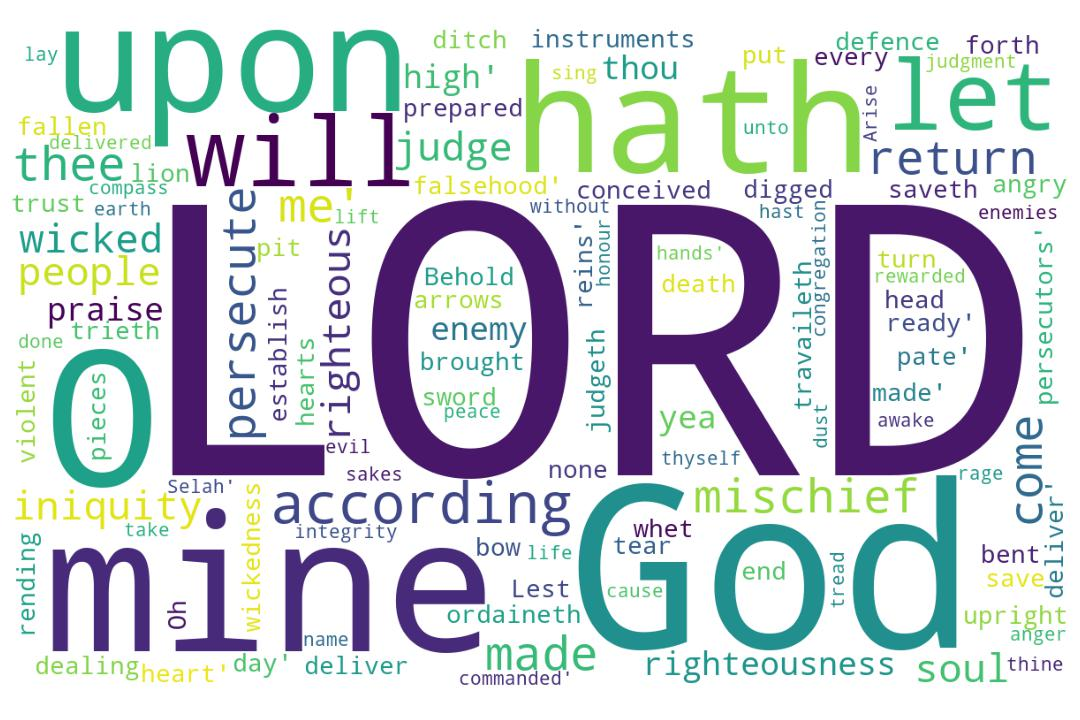
\includegraphics[width=\linewidth]{19OT-Psalms/Psalm7-WordCloud.jpg}
  \caption{Psalm 7 Word Cloud}
  \label{fig:Psalm 7 word Cloud}
\end{figure}



\marginpar{\scriptsize \centering \fcolorbox{bone}{lime}{\textbf{ABOUT DISTRESS}}\\
 \fcolorbox{bone}{lime}{\textbf{\& DELIVERANCE}} \\ (Psalm 7:1-17) \begin{compactenum}[I.][8]
    \item \textbf{Recognizes Sin and its Damage}
    \item \textbf{Reaches a State of Despair}
    \item \textbf{Remembers the Source of his Deliverance}
    \item \textbf{Repeats his Sorrow and Distress}
    \item \textbf{Recounts the Sum of Adversaries}
    \item \textbf{Requests Sinners to Departs}
    \item \textbf{Rejoices in his Savior and Deliverer}
\end{compactenum}}

\marginpar{\scriptsize \centering \fcolorbox{bone}{yellow}{\textbf{ACCUSED}}\\
 \fcolorbox{bone}{yellow}{\textbf{\& APPEALING}} \\ (Psalm 7:1-17) \begin{compactenum}[I.][8]
    \item The \textbf{First Appeal} \index[scripture]{Psalms!Psa 007:001} (Psa 7:1)
    \item A \textbf{False Accusation} \index[scripture]{Psalms!Psa 007:003} (Psa 7:3)
    \item \textbf{Fitting Amends} \index[scripture]{Psalms!Psa 007:005} (Psa 7:5)
    \item \textbf{Fierce Anger} \index[scripture]{Psalms!Psa 007:006} (Psa 7:6)
    \item A \textbf{Final Accounting} \index[scripture]{Psalms!Psa 007:008} (Psa 7:8)
    \item \textbf{Full Assurance} \index[scripture]{Psalms!Psa 007:010} (Psa 7:10)
    \item The \textbf{Final Annihilation} \index[scripture]{Psalms!Psa 007:016} (Psa 7:16)
\end{compactenum}}

\footnote{\textcolor[cmyk]{0.99998,1,0,0}{\hyperlink{TOC}{Return to end of Table of Contents.}}}\footnote{\href{https://audiobible.com/bible/bible.html}{\textcolor[cmyk]{0.99998,1,0,0}{Psalms Audio}}}\textcolor[cmyk]{0.99998,1,0,0}{Shiggaion of David, which he sang unto the LORD, concerning the words of Cush the Benjamite.}\\
\\
\textcolor[cmyk]{0.99998,1,0,0}{O LORD my God, in thee do I put my trust: save me from all them that persecute me, and deliver me:}
[2] \textcolor[cmyk]{0.99998,1,0,0}{Lest he tear my soul like a lion, rending \emph{it} in pieces, while \emph{there} \emph{is} none to deliver.}
[3] \textcolor[cmyk]{0.99998,1,0,0}{O LORD my God, if I have done this; if there be iniquity in my hands;}
[4] \textcolor[cmyk]{0.99998,1,0,0}{If I have rewarded evil unto him that was at peace with me; (yea, I have delivered him that without cause is mine enemy:)}
[5] \textcolor[cmyk]{0.99998,1,0,0}{Let the enemy persecute my soul, and take \emph{it}; yea, let him tread down my life upon the earth, and lay mine honour in the dust. Selah.}
[6] \textcolor[cmyk]{0.99998,1,0,0}{Arise, O LORD, in thine anger, lift up thyself because of the rage of mine enemies: and awake for me \emph{to} the judgment \emph{that} thou hast commanded.}
[7] \textcolor[cmyk]{0.99998,1,0,0}{So shall the congregation of the people compass thee about: for their sakes therefore return thou on high.}
[8] \textcolor[cmyk]{0.99998,1,0,0}{The LORD shall judge the people: judge me, O LORD, according to my righteousness, and according to mine integrity \emph{that} \emph{is} in me.}
[9] \textcolor[cmyk]{0.99998,1,0,0}{Oh\ let the wickedness of the wicked come to an end; but establish the just: for the righteous God trieth the hearts and reins.}
[10] \textcolor[cmyk]{0.99998,1,0,0}{My defence \emph{is} of God, which saveth the upright in heart.}
[11] \textcolor[cmyk]{0.99998,1,0,0}{God judgeth the righteous, and God is angry \emph{with} \emph{the} \emph{wicked} every day.}
[12] \textcolor[cmyk]{0.99998,1,0,0}{If he turn not, he will whet his sword; he hath bent his bow, and made it ready.}
[13] \textcolor[cmyk]{0.99998,1,0,0}{He hath also prepared for him the instruments of death; he ordaineth his arrows against the persecutors.}
[14] \textcolor[cmyk]{0.99998,1,0,0}{Behold, he travaileth with iniquity, and hath conceived mischief, and brought forth falsehood.}
[15] \textcolor[cmyk]{0.99998,1,0,0}{He made a pit, and digged it, and is fallen into the ditch \emph{which} he made.}
[16] \textcolor[cmyk]{0.99998,1,0,0}{His mischief shall return upon his own head, and his violent dealing shall come down upon his own pate.}\footnote{\textbf{Genesis 3:15} - And I will put enmity between thee and the woman, and between thy seed and her seed; it shall bruise thy head, and thou shalt bruise his heel.}
[17] \textcolor[cmyk]{0.99998,1,0,0}{I will praise the LORD according to his righteousness: and will sing praise to the name of the LORD most high.}


\section{Psalm 7 Comments}




%\input{19OT-Psalms/Psalm7-WordIndex}
\section{Psalm 7 Outlines}

\subsection{My Outlines}

\subsubsection{A Psalm about Distress and Deliverance}

\index[speaker]{Keith Anthony!Psalm 007 (A Psalm about Distress and Deliverance)}
\index[series]{Psalms (Keith Anthony)!Psalm 007 (A Psalm about Distress and Deliverance)}
\index[date]{unknown!Psalm 007 (A Psalm about Distress and Deliverance) (Keith Anthony)}
\begin{compactenum}[I.]
    \item \textbf{Recognizes Sin and its Damage}
    \item \textbf{Reaches a State of Despair}
    \item \textbf{Remembers the Source of his Deliverance}
    \item \textbf{Repeats his Sorrow and Distress}
    \item \textbf{Recounts the Sum of Adversaries}
    \item \textbf{Requests Sinners to Departs}
    \item \textbf{Rejoices in his Savior and Deliverer}
\end{compactenum}


\subsubsection{Accused and Appealing}

\index[speaker]{Keith Anthony!Psalm 007 (Accused and Appealing)}
\index[series]{Psalms (Keith Anthony)!Psalm 007 (Accused and Appealing)}
\index[date]{2020/06/27!Psalm 007 (Accused and Appealing) (Keith Anthony)}
\begin{compactenum}[I.]

    \item The \textbf{First Appeal} \index[scripture]{Psalms!Psa 007:001} (Psa 7:1)
    \item A \textbf{False Accusation} \index[scripture]{Psalms!Psa 007:003} (Psa 7:3)
    \item \textbf{Fitting Amends} \index[scripture]{Psalms!Psa 007:005} (Psa 7:5)
    \item \textbf{Fierce Anger} \index[scripture]{Psalms!Psa 007:006} (Psa 7:6)
    \item A \textbf{Final Accounting} \index[scripture]{Psalms!Psa 007:008} (Psa 7:8)
    \item \textbf{Full Assurance} \index[scripture]{Psalms!Psa 007:010} (Psa 7:10)
    \item The \textbf{Final Annihilation} \index[scripture]{Psalms!Psa 007:016} (Psa 7:16)
\end{compactenum}
\subsection{Outlines from Others}


%\section{Psalm 7 Statistics}

%%%%%%%%%%%%%%%%%%%%%%%%%%%
%%%%%Word Statistics
%%%%%%%%%%%%%%%%%%%%%%%%%%%


\normalsize



\subsection{Chapter Word Statistics}


%%%%%%%%%%
%%%%%%%%%%
 
\begin{center}
\begin{longtable}{l|c|c|c|c}
\caption[Stats for Psalm 7]{Stats for Psalm 7} \label{table:Stats for Psalm 7} \\ 
\hline \multicolumn{1}{|c|}{\textbf{Verse(s)}} & \multicolumn{1}{|c|}{\textbf{Count}} & \multicolumn{1}{|c|}{\textbf{Unique}} & \multicolumn{1}{|c|}{\textbf{Italics}} & \multicolumn{1}{|c|}{\textbf{Uniq Italic}}  \\ \hline 
\endfirsthead
 
\multicolumn{5}{c}
{{\bfseries \tablename\ \thetable{} -- continued from previous page}} \\  
\hline \multicolumn{1}{|c|}{\textbf{Verse(s)}} & \multicolumn{1}{|c|}{\textbf{Count}} & \multicolumn{1}{|c|}{\textbf{Unique}} & \multicolumn{1}{|c|}{\textbf{Italics}} & \multicolumn{1}{|c|}{\textbf{Uniq Italic}}  \\ \hline 
\endhead
 
\hline \multicolumn{5}{|r|}{{Continued if needed}} \\ \hline
\endfoot 
1 & 22 & 19 & 0 & 0\\ \hline
2 & 18 & 18 & 3 & 3\\ \hline
3 & 16 & 14 & 0 & 0\\ \hline
4 & 24 & 20 & 0 & 0\\ \hline
5 & 27 & 23 & 1 & 1\\ \hline
6 & 27 & 25 & 2 & 2\\ \hline
7 & 18 & 17 & 0 & 0\\ \hline
8 & 23 & 18 & 2 & 2\\ \hline
9 & 24 & 20 & 0 & 0\\ \hline
10 & 11 & 11 & 1 & 1\\ \hline
11 & 13 & 12 & 3 & 3\\ \hline
12 & 18 & 15 & 0 & 0\\ \hline
13 & 17 & 16 & 0 & 0\\ \hline
14 & 13 & 12 & 0 & 0\\ \hline
15 & 16 & 14 & 1 & 1\\ \hline
16 & 19 & 14 & 0 & 0\\ \hline
17 & 21 & 15 & 0 & 0\\ \hline
\hline \hline
Total & 327 & 176 & 13 & 9



\end{longtable}
\end{center}

%%%%%%%%%%
%%%%%%%%%%
 
\subsection{Words by Frequency}

\begin{center}
\begin{longtable}{l|r}
\caption[Word Frequencies in Psalm 7]{Word Frequencies in Psalm 7} \label{table:WordsIn-Psalm-7} \\ 
\hline \multicolumn{1}{|c|}{\textbf{Word}} & \multicolumn{1}{c|}{\textbf{Frequency}} \\ \hline 
\endfirsthead
 
\multicolumn{2}{c}
{{\bfseries \tablename\ \thetable{} -- continued from previous page}} \\ 
\hline \multicolumn{1}{|c|}{\textbf{Word}} & \multicolumn{1}{c|}{\textbf{Frequency}} \\ \hline 
\endhead
 
\hline \multicolumn{2}{|r|}{{Continued if needed}} \\ \hline
\endfoot
 
\hline \hline
\endlastfoot
the & 21 \\ \hline
and & 14 \\ \hline
my & 8 \\ \hline
LORD & 7 \\ \hline
in & 7 \\ \hline
me & 7 \\ \hline
he & 7 \\ \hline
of & 7 \\ \hline
his & 7 \\ \hline
God & 6 \\ \hline
to & 6 \\ \hline
I & 5 \\ \hline
O & 4 \\ \hline
him & 4 \\ \hline
mine & 4 \\ \hline
for & 4 \\ \hline
shall & 4 \\ \hline
that & 3 \\ \hline
\emph{is} & 3 \\ \hline
have & 3 \\ \hline
is & 3 \\ \hline
upon & 3 \\ \hline
according & 3 \\ \hline
will & 3 \\ \hline
hath & 3 \\ \hline
made & 3 \\ \hline
thee & 2 \\ \hline
persecute & 2 \\ \hline
deliver & 2 \\ \hline
soul & 2 \\ \hline
a & 2 \\ \hline
\emph{it} & 2 \\ \hline
if & 2 \\ \hline
iniquity & 2 \\ \hline
If & 2 \\ \hline
with & 2 \\ \hline
yea & 2 \\ \hline
enemy & 2 \\ \hline
let & 2 \\ \hline
down & 2 \\ \hline
\emph{that} & 2 \\ \hline
thou & 2 \\ \hline
people & 2 \\ \hline
return & 2 \\ \hline
high & 2 \\ \hline
judge & 2 \\ \hline
righteousness & 2 \\ \hline
come & 2 \\ \hline
righteous & 2 \\ \hline
it & 2 \\ \hline
He & 2 \\ \hline
mischief & 2 \\ \hline
own & 2 \\ \hline
praise & 2 \\ \hline
do & 1 \\ \hline
put & 1 \\ \hline
trust & 1 \\ \hline
save & 1 \\ \hline
from & 1 \\ \hline
all & 1 \\ \hline
them & 1 \\ \hline
Lest & 1 \\ \hline
tear & 1 \\ \hline
like & 1 \\ \hline
lion & 1 \\ \hline
rending & 1 \\ \hline
pieces & 1 \\ \hline
while & 1 \\ \hline
\emph{there} & 1 \\ \hline
none & 1 \\ \hline
done & 1 \\ \hline
this & 1 \\ \hline
there & 1 \\ \hline
be & 1 \\ \hline
hands & 1 \\ \hline
rewarded & 1 \\ \hline
evil & 1 \\ \hline
unto & 1 \\ \hline
was & 1 \\ \hline
at & 1 \\ \hline
peace & 1 \\ \hline
delivered & 1 \\ \hline
without & 1 \\ \hline
cause & 1 \\ \hline
Let & 1 \\ \hline
take & 1 \\ \hline
tread & 1 \\ \hline
life & 1 \\ \hline
earth & 1 \\ \hline
lay & 1 \\ \hline
honour & 1 \\ \hline
dust & 1 \\ \hline
Selah & 1 \\ \hline
Arise & 1 \\ \hline
thine & 1 \\ \hline
anger & 1 \\ \hline
lift & 1 \\ \hline
up & 1 \\ \hline
thyself & 1 \\ \hline
because & 1 \\ \hline
rage & 1 \\ \hline
enemies & 1 \\ \hline
awake & 1 \\ \hline
\emph{to} & 1 \\ \hline
judgment & 1 \\ \hline
hast & 1 \\ \hline
commanded & 1 \\ \hline
So & 1 \\ \hline
congregation & 1 \\ \hline
compass & 1 \\ \hline
about & 1 \\ \hline
their & 1 \\ \hline
sakes & 1 \\ \hline
therefore & 1 \\ \hline
on & 1 \\ \hline
The & 1 \\ \hline
integrity & 1 \\ \hline
Oh & 1 \\ \hline
wickedness & 1 \\ \hline
wicked & 1 \\ \hline
an & 1 \\ \hline
end & 1 \\ \hline
but & 1 \\ \hline
establish & 1 \\ \hline
just & 1 \\ \hline
trieth & 1 \\ \hline
hearts & 1 \\ \hline
reins & 1 \\ \hline
My & 1 \\ \hline
defence & 1 \\ \hline
which & 1 \\ \hline
saveth & 1 \\ \hline
upright & 1 \\ \hline
heart & 1 \\ \hline
judgeth & 1 \\ \hline
angry & 1 \\ \hline
\emph{with} & 1 \\ \hline
\emph{the} & 1 \\ \hline
\emph{wicked} & 1 \\ \hline
every & 1 \\ \hline
day & 1 \\ \hline
turn & 1 \\ \hline
not & 1 \\ \hline
whet & 1 \\ \hline
sword & 1 \\ \hline
bent & 1 \\ \hline
bow & 1 \\ \hline
ready & 1 \\ \hline
also & 1 \\ \hline
prepared & 1 \\ \hline
instruments & 1 \\ \hline
death & 1 \\ \hline
ordaineth & 1 \\ \hline
arrows & 1 \\ \hline
against & 1 \\ \hline
persecutors & 1 \\ \hline
Behold & 1 \\ \hline
travaileth & 1 \\ \hline
conceived & 1 \\ \hline
brought & 1 \\ \hline
forth & 1 \\ \hline
falsehood & 1 \\ \hline
pit & 1 \\ \hline
digged & 1 \\ \hline
fallen & 1 \\ \hline
into & 1 \\ \hline
ditch & 1 \\ \hline
\emph{which} & 1 \\ \hline
His & 1 \\ \hline
head & 1 \\ \hline
violent & 1 \\ \hline
dealing & 1 \\ \hline
pate & 1 \\ \hline
sing & 1 \\ \hline
name & 1 \\ \hline
most & 1 \\ \hline
\end{longtable}
\end{center}



\normalsize



\subsection{Words Alphabetically}

\begin{center}
\begin{longtable}{l|r}
\caption[Word Alphabetically in Psalm 7]{Word Alphabetically in Psalm 7} \label{table:WordsIn-Psalm-7} \\ 
\hline \multicolumn{1}{|c|}{\textbf{Word}} & \multicolumn{1}{c|}{\textbf{Frequency}} \\ \hline 
\endfirsthead
 
\multicolumn{2}{c}
{{\bfseries \tablename\ \thetable{} -- continued from previous page}} \\ 
\hline \multicolumn{1}{|c|}{\textbf{Word}} & \multicolumn{1}{c|}{\textbf{Frequency}} \\ \hline 
\endhead
 
\hline \multicolumn{2}{|r|}{{Continued if needed}} \\ \hline
\endfoot
 
\hline \hline
\endlastfoot
Arise & 1 \\ \hline
Behold & 1 \\ \hline
God & 6 \\ \hline
He & 2 \\ \hline
His & 1 \\ \hline
I & 5 \\ \hline
If & 2 \\ \hline
LORD & 7 \\ \hline
Lest & 1 \\ \hline
Let & 1 \\ \hline
My & 1 \\ \hline
O & 4 \\ \hline
Oh & 1 \\ \hline
Selah & 1 \\ \hline
So & 1 \\ \hline
The & 1 \\ \hline
\emph{is} & 3 \\ \hline
\emph{it} & 2 \\ \hline
\emph{that} & 2 \\ \hline
\emph{there} & 1 \\ \hline
\emph{the} & 1 \\ \hline
\emph{to} & 1 \\ \hline
\emph{which} & 1 \\ \hline
\emph{wicked} & 1 \\ \hline
\emph{with} & 1 \\ \hline
a & 2 \\ \hline
about & 1 \\ \hline
according & 3 \\ \hline
against & 1 \\ \hline
all & 1 \\ \hline
also & 1 \\ \hline
an & 1 \\ \hline
and & 14 \\ \hline
anger & 1 \\ \hline
angry & 1 \\ \hline
arrows & 1 \\ \hline
at & 1 \\ \hline
awake & 1 \\ \hline
be & 1 \\ \hline
because & 1 \\ \hline
bent & 1 \\ \hline
bow & 1 \\ \hline
brought & 1 \\ \hline
but & 1 \\ \hline
cause & 1 \\ \hline
come & 2 \\ \hline
commanded & 1 \\ \hline
compass & 1 \\ \hline
conceived & 1 \\ \hline
congregation & 1 \\ \hline
day & 1 \\ \hline
dealing & 1 \\ \hline
death & 1 \\ \hline
defence & 1 \\ \hline
deliver & 2 \\ \hline
delivered & 1 \\ \hline
digged & 1 \\ \hline
ditch & 1 \\ \hline
do & 1 \\ \hline
done & 1 \\ \hline
down & 2 \\ \hline
dust & 1 \\ \hline
earth & 1 \\ \hline
end & 1 \\ \hline
enemies & 1 \\ \hline
enemy & 2 \\ \hline
establish & 1 \\ \hline
every & 1 \\ \hline
evil & 1 \\ \hline
fallen & 1 \\ \hline
falsehood & 1 \\ \hline
for & 4 \\ \hline
forth & 1 \\ \hline
from & 1 \\ \hline
hands & 1 \\ \hline
hast & 1 \\ \hline
hath & 3 \\ \hline
have & 3 \\ \hline
he & 7 \\ \hline
head & 1 \\ \hline
heart & 1 \\ \hline
hearts & 1 \\ \hline
high & 2 \\ \hline
him & 4 \\ \hline
his & 7 \\ \hline
honour & 1 \\ \hline
if & 2 \\ \hline
in & 7 \\ \hline
iniquity & 2 \\ \hline
instruments & 1 \\ \hline
integrity & 1 \\ \hline
into & 1 \\ \hline
is & 3 \\ \hline
it & 2 \\ \hline
judge & 2 \\ \hline
judgeth & 1 \\ \hline
judgment & 1 \\ \hline
just & 1 \\ \hline
lay & 1 \\ \hline
let & 2 \\ \hline
life & 1 \\ \hline
lift & 1 \\ \hline
like & 1 \\ \hline
lion & 1 \\ \hline
made & 3 \\ \hline
me & 7 \\ \hline
mine & 4 \\ \hline
mischief & 2 \\ \hline
most & 1 \\ \hline
my & 8 \\ \hline
name & 1 \\ \hline
none & 1 \\ \hline
not & 1 \\ \hline
of & 7 \\ \hline
on & 1 \\ \hline
ordaineth & 1 \\ \hline
own & 2 \\ \hline
pate & 1 \\ \hline
peace & 1 \\ \hline
people & 2 \\ \hline
persecute & 2 \\ \hline
persecutors & 1 \\ \hline
pieces & 1 \\ \hline
pit & 1 \\ \hline
praise & 2 \\ \hline
prepared & 1 \\ \hline
put & 1 \\ \hline
rage & 1 \\ \hline
ready & 1 \\ \hline
reins & 1 \\ \hline
rending & 1 \\ \hline
return & 2 \\ \hline
rewarded & 1 \\ \hline
righteous & 2 \\ \hline
righteousness & 2 \\ \hline
sakes & 1 \\ \hline
save & 1 \\ \hline
saveth & 1 \\ \hline
shall & 4 \\ \hline
sing & 1 \\ \hline
soul & 2 \\ \hline
sword & 1 \\ \hline
take & 1 \\ \hline
tear & 1 \\ \hline
that & 3 \\ \hline
the & 21 \\ \hline
thee & 2 \\ \hline
their & 1 \\ \hline
them & 1 \\ \hline
there & 1 \\ \hline
therefore & 1 \\ \hline
thine & 1 \\ \hline
this & 1 \\ \hline
thou & 2 \\ \hline
thyself & 1 \\ \hline
to & 6 \\ \hline
travaileth & 1 \\ \hline
tread & 1 \\ \hline
trieth & 1 \\ \hline
trust & 1 \\ \hline
turn & 1 \\ \hline
unto & 1 \\ \hline
up & 1 \\ \hline
upon & 3 \\ \hline
upright & 1 \\ \hline
violent & 1 \\ \hline
was & 1 \\ \hline
whet & 1 \\ \hline
which & 1 \\ \hline
while & 1 \\ \hline
wicked & 1 \\ \hline
wickedness & 1 \\ \hline
will & 3 \\ \hline
with & 2 \\ \hline
without & 1 \\ \hline
yea & 2 \\ \hline
\end{longtable}
\end{center}



\normalsize



\subsection{Word Lengths in Chapter}
\normalsize
\begin{longtable}{l|p{3.75in}}
\caption[Words by Length in Psalm 7]{Words by Length in Psalm 7} \label{table:WordsIn-Psalm-7} \\ 
\hline \multicolumn{1}{|c|}{\textbf{Length}} & \multicolumn{1}{c|}{\textbf{Words}} \\ \hline 
\endfirsthead
 
\multicolumn{2}{c}
{{\bfseries \tablename\ \thetable{} -- continued from previous page}} \\ 
\hline \multicolumn{1}{|c|}{\textbf{Length}} & \multicolumn{1}{c|}{\textbf{Words}} \\ \hline 
\endhead
 
\hline \multicolumn{2}{|r|}{{Continued if needed}} \\ \hline
\endfoot
 
\hline \hline
\endlastfoot
1 & O, I, a \\ \hline
2 & my, in, do, me, he, \emph{it}, \emph{is}, to, if, be, If, at, is, up, of, \emph{to}, So, on, Oh, an, My, it, He \\ \hline
3 & God, put, all, and, him, was, yea, Let, the, let, lay, for, The, end, but, \emph{the}, day, not, his, bow, pit, His, own \\ \hline
4 & LORD, thee, save, from, them, that, Lest, tear, soul, like, lion, none, have, done, this, evil, unto, with, mine, take, down, life, upon, dust, lift, rage, \emph{that}, thou, hast, high, come, just, \emph{with}, turn, will, whet, hath, bent, made, also, into, head, pate, sing, name, most \\ \hline
5 & trust, while, \emph{there}, there, hands, peace, cause, enemy, tread, earth, Selah, Arise, thine, anger, awake, shall, about, their, sakes, judge, reins, which, heart, angry, every, sword, ready, death, forth, ditch, \emph{which} \\ \hline
6 & pieces, honour, people, return, wicked, trieth, hearts, saveth, \emph{wicked}, arrows, Behold, digged, fallen, praise \\ \hline
7 & deliver, rending, without, thyself, because, enemies, compass, defence, upright, judgeth, against, brought, violent, dealing \\ \hline
8 & iniquity, rewarded, judgment, prepared, mischief \\ \hline
9 & persecute, delivered, commanded, therefore, according, integrity, establish, righteous, ordaineth, conceived, falsehood \\ \hline
10 & wickedness, travaileth \\ \hline
11 & instruments, persecutors \\ \hline
12 & congregation \\ \hline
13 & righteousness \\ \hline
\end{longtable}






%%%%%%%%%%
%%%%%%%%%%
 



%%%%%%%%%%
%%%%%%%%%%
\subsection{Verses with 13 Words in Chapter}
\normalsize
\begin{longtable}{l|p{3.75in}}
\caption[Verses with 13 Words  in Psalm 7]{Verses with 13 Words  in Psalm 7} \label{table:Verses with 13 Words in-Psalm-7} \\ 
\hline \multicolumn{1}{|c|}{\textbf{Reference}} & \multicolumn{1}{c|}{\textbf{Verse}} \\ \hline 
\endfirsthead
 
\multicolumn{2}{c}
{{\bfseries \tablename\ \thetable{} -- continued from previous page}} \\ 
\hline \multicolumn{1}{|c|}{\textbf{Reference}} & \multicolumn{1}{c|}{\textbf{Verse}} \\ \hline 
\endhead
 
\hline \multicolumn{2}{|r|}{{Continued if needed}} \\ \hline
\endfoot
 
\hline \hline
\endlastfoot
Psalms 07:11 & God judgeth the righteous, and God is angry \emph{with} \emph{the} \emph{wicked} every day. \\ \hline
Psalms 07:14 & Behold, he travaileth with iniquity, and hath conceived mischief, and brought forth falsehood. \\ \hline
\end{longtable}






%%%%%%%%%%
%%%%%%%%%%
 



%%%%%%%%%%
%%%%%%%%%%
\subsection{Verses with 18 Words in Chapter}
\normalsize
\begin{longtable}{l|p{3.75in}}
\caption[Verses with 18 Words  in Psalm 7]{Verses with 18 Words  in Psalm 7} \label{table:Verses with 18 Words in-Psalm-7} \\ 
\hline \multicolumn{1}{|c|}{\textbf{Reference}} & \multicolumn{1}{c|}{\textbf{Verse}} \\ \hline 
\endfirsthead
 
\multicolumn{2}{c}
{{\bfseries \tablename\ \thetable{} -- continued from previous page}} \\ 
\hline \multicolumn{1}{|c|}{\textbf{Reference}} & \multicolumn{1}{c|}{\textbf{Verse}} \\ \hline 
\endhead
 
\hline \multicolumn{2}{|r|}{{Continued if needed}} \\ \hline
\endfoot
 
\hline \hline
\endlastfoot
Psalms 07:2 & Lest he tear my soul like a lion, rending \emph{it} in pieces, while \emph{there} \emph{is} none to deliver. \\ \hline
Psalms 07:7 & So shall the congregation of the people compass thee about: for their sakes therefore return thou on high. \\ \hline
Psalms 07:12 & If he turn not, he will whet his sword; he hath bent his bow, and made it ready. \\ \hline
\end{longtable}






%%%%%%%%%%
%%%%%%%%%%
\subsection{Psalm 7 Repeated Phrases}


%%%%%%%%%%
%%%%%%%%%%
\normalsize
 
\begin{center}
\begin{longtable}{|p{3.0in}|p{0.5in}|}
\caption[Psalm 7 Repeated Phrases]{Psalm 7 Repeated Phrases}\label{table:Repeated Phrases Psalm 7} \\
\hline \multicolumn{1}{|c|}{\textbf{Phrase}} & \multicolumn{1}{c|}{\textbf{Frequency}} \\ \hline 
\endfirsthead
 
\multicolumn{2}{c}
{{\bfseries \tablename\ \thetable{} -- continued from previous page}} \\  
\hline \multicolumn{1}{|c|}{\textbf{Phrase}} & \multicolumn{1}{c|}{\textbf{Frequency}} \\ \hline 
\endhead
 
\hline \multicolumn{2}{c}{{ }} \\ \hline
\endfoot 
O LORD & 4\\ \hline 
of the & 4\\ \hline 
I have & 3\\ \hline 
according to & 3\\ \hline 
\end{longtable}
\end{center}



%%%%%%%%%%
%%%%%%%%%%




\chapter{Psalm 8}

\begin{figure}
  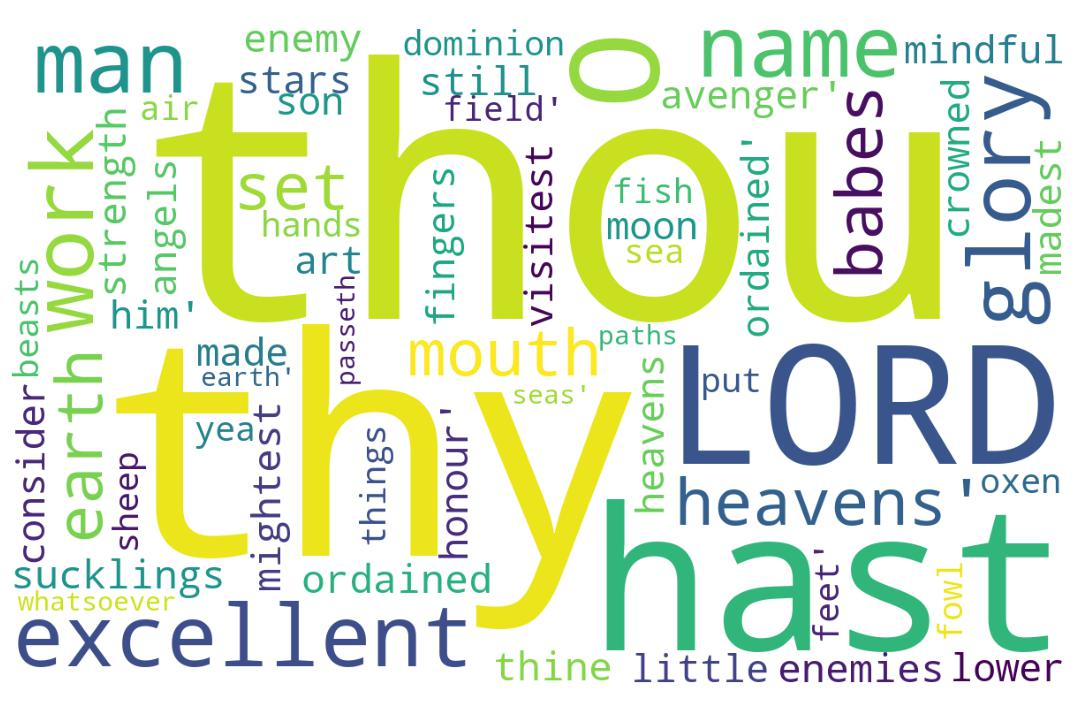
\includegraphics[width=\linewidth]{19OT-Psalms/Psalm8-WordCloud.jpg}
  \caption{Psalm 8 Word Cloud}
  \label{fig:Psalm 8 word Cloud}
\end{figure}

\marginpar{\scriptsize \centering \fcolorbox{bone}{lime}{\textbf{THAT EXCELLENT NAME}}\\ (Psalm 8:1-9) \begin{compactenum}[I.][8]
    \item The \textbf{Praise of Babes} \index[scripture]{Psalms!Psa 008:02} (Psa 8:2)
    \item \textbf{Power to Man} \index[scripture]{Psalms!Psa 008:02} (Psa 8:2)
    \item The \textbf{Place of Men} \index[scripture]{Psalms!Psa 008:04} (Psa 8:4)
    \item \textbf{Power over Creation} \index[scripture]{Psalms!Psa 008:06} (Psa 8:6)
    \item The \textbf{Paths of the Seas} \index[scripture]{Psalms!Psa 008:08} (Psa 8:8)
    \item The \textbf{Passing of Creatures} \index[scripture]{Psalms!Psa 008:08} (Psa 8:8)
    \item The \textbf{Presence of a Name} \index[scripture]{Psalms!Psa 008:09} (Psa 8:9)
\end{compactenum}}

% \textcolor{jungle}{$_{3112}^{207}$} TEMPLATE

\footnote{\textcolor[cmyk]{0.99998,1,0,0}{\hyperlink{TOC}{Return to end of Table of Contents.}}}\footnote{\href{https://audiobible.com/bible/bible.html}{\textcolor[cmyk]{0.99998,1,0,0}{Psalms Audio}}}\textcolor[cmyk]{0.99998,1,0,0}{To the chief Musician upon Gittith, A Psalm of David.}\\
\\
\textcolor[cmyk]{0.99998,1,0,0}{O\textcolor{jungle}{$_{1372}^{1}$} LORD our Lord, how excellent \emph{is} thy name in all the earth! who hast set thy glory above the heavens.}
[2] \textcolor[cmyk]{0.99998,1,0,0}{Out\textcolor{jungle}{$_{1393}^{22}$} of the \fcolorbox{bone}{lime}{mouth of babes} and sucklings hast thou ordained strength because of thine enemies, that thou mightest \fcolorbox{bone}{lime}{still the enemy} and the avenger.}\footnote{\textbf{Matthew 21:16} -  And said unto him, Hearest thou what these say? And Jesus saith unto them, Yea; have ye never read, Out of the mouth of babes and sucklings thou hast perfected praise?}
[3] \textcolor[cmyk]{0.99998,1,0,0}{When\textcolor{jungle}{$_{1418}^{27}$} I consider thy heavens, the work of thy fingers, the moon and the stars, which thou hast ordained;}\footnote{\textbf{Psalm 102:25} - Of old hast thou laid the foundation of the earth: and the heavens are the work of thy hands.}\footnote{\textbf{Psalm 143:5} - I remember the days of old; I meditate on all thy works; I muse on the work of thy hands.}\footnote{\textbf{Isaiah 64:8} - But now, O LORD, thou art our father; we are the clay, and thou our potter; and we all are the work of thy hand.}
[4] \textcolor[cmyk]{0.99998,1,0,0}{\fcolorbox{bone}{lime}{What\textcolor{jungle}{$_{1437}^{66}$} is man}, that thou art mindful of him? and the son of man, that thou visitest him?}\footnote{\textbf{Job 7:17} - What is man, that thou shouldest magnify him? and that thou shouldest set thine heart upon him?}\footnote{\textbf{Job 15:14} - What is man, that he should be clean? and he which is born of a woman, that he should be righteous?}\footnote{\textbf{Psalm 144:3} - LORD, what is man, that thou takest knowledge of him! or the son of man, that thou makest account of him!}\footnote{\textbf{Hebrews 2:6} - But one in a certain place testified, saying, What is man, that thou art mindful of him? or the son of man, that thou visitest him?}
[5] \textcolor[cmyk]{0.99998,1,0,0}{For\textcolor{jungle}{$_{1455}^{84}$} thou hast made him a little lower than the angels, and hast crowned him with glory and honour.}
[6] \textcolor[cmyk]{0.99998,1,0,0}{Thou\textcolor{jungle}{$_{1474}^{103}$} madest him to have dominion over the works of thy hands; thou hast put all \emph{things} \fcolorbox{bone}{lime}{under his feet}:}\footnote{\textbf{Genesis 1:26-28} - And God said, Let us make man in our image, after our likeness: and let them have dominion over the fish of the sea, and over the fowl of the air, and over the cattle, and over all the earth, and over every creeping thing that creepeth upon the earth. [27] So God created man in his own image, in the image of God created he him; male and female created he them. [28] And God blessed them, and God said unto them, Be fruitful, and multiply, and replenish the earth, and subdue it: and have dominion over the fish of the sea, and over the fowl of the air, and over every living thing that moveth upon the earth.}
[7] \textcolor[cmyk]{0.99998,1,0,0}{All\textcolor{jungle}{$_{1494}^{123}$} sheep and oxen, yea, and the beasts of the field;}
[8] \textcolor[cmyk]{0.99998,1,0,0}{The\textcolor{jungle}{$_{1505}^{134}$} fowl of the air, and the fish of the sea, \emph{and} \emph{whatsoever} \fcolorbox{bone}{lime}{passeth} through the \fcolorbox{bone}{lime}{paths of the seas}.}
[9] \textcolor[cmyk]{0.99998,1,0,0}{O\textcolor{jungle}{$_{1525}^{154}$} LORD our Lord, how excellent \emph{is} \fcolorbox{bone}{lime}{thy name} in all the earth\textcolor{jungle}{$_{1537}^{166}$}!}\footnote{But, putting things in perspective, God's word is magnified even above God's name: See Psalm 138:2 - I will worship toward thy holy temple, and praise thy name for thy lovingkindness and for thy truth: for thou hast magnified thy word above all thy name.}\footnote{\textbf{Job 37:23} - Touching the Almighty, we cannot find him out: he is excellent in power, and in judgment, and in plenty of justice: he will not afflict.}


\section{Psalm 8 Comments}


%\index[NWIV]{21!Psalms!Psa 8:1}\index[AWIP]{O!Psalms!Psa 8:1}\index[AWIP]{LORD!Psalms!Psa 8:1}\index[AWIP]{our!Psalms!Psa 8:1}\index[AWIP]{Lord!Psalms!Psa 8:1}\index[AWIP]{how!Psalms!Psa 8:1}\index[AWIP]{excellent!Psalms!Psa 8:1}\index[AWIP]{\emph{is}!Psalms!Psa 8:1}\index[AWIP]{thy!Psalms!Psa 8:1}\index[AWIP]{thy!Psalms!Psa 8:1 (2)}\index[AWIP]{name!Psalms!Psa 8:1}\index[AWIP]{in!Psalms!Psa 8:1}\index[AWIP]{all!Psalms!Psa 8:1}\index[AWIP]{the!Psalms!Psa 8:1}\index[AWIP]{the!Psalms!Psa 8:1 (2)}\index[AWIP]{earth!!Psalms!Psa 8:1}\index[AWIP]{who!Psalms!Psa 8:1}\index[AWIP]{hast!Psalms!Psa 8:1}\index[AWIP]{set!Psalms!Psa 8:1}\index[AWIP]{glory!Psalms!Psa 8:1}\index[AWIP]{above!Psalms!Psa 8:1}\index[AWIP]{heavens!Psalms!Psa 8:1}\index[AWIP]{\emph{is}!Psalms!Psa 8:1}

\index[NWIV]{25!Psalms!Psa 8:2}\index[AWIP]{Out!Psalms!Psa 8:2}\index[AWIP]{of!Psalms!Psa 8:2}\index[AWIP]{of!Psalms!Psa 8:2 (2)}\index[AWIP]{of!Psalms!Psa 8:2 (3)}\index[AWIP]{the!Psalms!Psa 8:2}\index[AWIP]{the!Psalms!Psa 8:2 (2)}\index[AWIP]{the!Psalms!Psa 8:2 (3)}\index[AWIP]{mouth!Psalms!Psa 8:2}\index[AWIP]{babes!Psalms!Psa 8:2}\index[AWIP]{and!Psalms!Psa 8:2}\index[AWIP]{and!Psalms!Psa 8:2 (2)}\index[AWIP]{sucklings!Psalms!Psa 8:2}\index[AWIP]{hast!Psalms!Psa 8:2}\index[AWIP]{thou!Psalms!Psa 8:2}\index[AWIP]{thou!Psalms!Psa 8:2 (2)}\index[AWIP]{ordained!Psalms!Psa 8:2}\index[AWIP]{strength!Psalms!Psa 8:2}\index[AWIP]{because!Psalms!Psa 8:2}\index[AWIP]{thine!Psalms!Psa 8:2}\index[AWIP]{enemies!Psalms!Psa 8:2}\index[AWIP]{that!Psalms!Psa 8:2}\index[AWIP]{mightest!Psalms!Psa 8:2}\index[AWIP]{still!Psalms!Psa 8:2}\index[AWIP]{enemy!Psalms!Psa 8:2}\index[AWIP]{avenger!Psalms!Psa 8:2}

\index[NWIV]{19!Psalms!Psa 8:3}\index[AWIP]{When!Psalms!Psa 8:3}\index[AWIP]{I!Psalms!Psa 8:3}\index[AWIP]{consider!Psalms!Psa 8:3}\index[AWIP]{thy!Psalms!Psa 8:3}\index[AWIP]{thy!Psalms!Psa 8:3 (2)}\index[AWIP]{heavens!Psalms!Psa 8:3}\index[AWIP]{the!Psalms!Psa 8:3}\index[AWIP]{the!Psalms!Psa 8:3 (2)}\index[AWIP]{the!Psalms!Psa 8:3 (3)}\index[AWIP]{work!Psalms!Psa 8:3}\index[AWIP]{of!Psalms!Psa 8:3}\index[AWIP]{fingers!Psalms!Psa 8:3}\index[AWIP]{moon!Psalms!Psa 8:3}\index[AWIP]{and!Psalms!Psa 8:3}\index[AWIP]{stars!Psalms!Psa 8:3}\index[AWIP]{which!Psalms!Psa 8:3}\index[AWIP]{thou!Psalms!Psa 8:3}\index[AWIP]{hast!Psalms!Psa 8:3}\index[AWIP]{ordained!Psalms!Psa 8:3}

\index[NWIV]{18!Psalms!Psa 8:4}\index[AWIP]{What!Psalms!Psa 8:4}\index[AWIP]{is!Psalms!Psa 8:4}\index[AWIP]{man!Psalms!Psa 8:4}\index[AWIP]{man!Psalms!Psa 8:4 (2)}\index[AWIP]{that!Psalms!Psa 8:4}\index[AWIP]{that!Psalms!Psa 8:4 (2)}\index[AWIP]{thou!Psalms!Psa 8:4}\index[AWIP]{thou!Psalms!Psa 8:4 (2)}\index[AWIP]{art!Psalms!Psa 8:4}\index[AWIP]{mindful!Psalms!Psa 8:4}\index[AWIP]{of!Psalms!Psa 8:4}\index[AWIP]{of!Psalms!Psa 8:4 (2)}\index[AWIP]{him?!Psalms!Psa 8:4}\index[AWIP]{him?!Psalms!Psa 8:4 (2)}\index[AWIP]{and!Psalms!Psa 8:4}\index[AWIP]{the!Psalms!Psa 8:4}\index[AWIP]{son!Psalms!Psa 8:4}\index[AWIP]{visitest!Psalms!Psa 8:4}

\index[NWIV]{19!Psalms!Psa 8:5}\index[AWIP]{For!Psalms!Psa 8:5}\index[AWIP]{thou!Psalms!Psa 8:5}\index[AWIP]{hast!Psalms!Psa 8:5}\index[AWIP]{hast!Psalms!Psa 8:5 (2)}\index[AWIP]{made!Psalms!Psa 8:5}\index[AWIP]{him!Psalms!Psa 8:5}\index[AWIP]{him!Psalms!Psa 8:5 (2)}\index[AWIP]{a!Psalms!Psa 8:5}\index[AWIP]{little!Psalms!Psa 8:5}\index[AWIP]{lower!Psalms!Psa 8:5}\index[AWIP]{than!Psalms!Psa 8:5}\index[AWIP]{the!Psalms!Psa 8:5}\index[AWIP]{angels!Psalms!Psa 8:5}\index[AWIP]{and!Psalms!Psa 8:5}\index[AWIP]{and!Psalms!Psa 8:5 (2)}\index[AWIP]{crowned!Psalms!Psa 8:5}\index[AWIP]{with!Psalms!Psa 8:5}\index[AWIP]{glory!Psalms!Psa 8:5}\index[AWIP]{honour!Psalms!Psa 8:5}

\index[NWIV]{20!Psalms!Psa 8:6}\index[AWIP]{Thou!Psalms!Psa 8:6}\index[AWIP]{madest!Psalms!Psa 8:6}\index[AWIP]{him!Psalms!Psa 8:6}\index[AWIP]{to!Psalms!Psa 8:6}\index[AWIP]{have!Psalms!Psa 8:6}\index[AWIP]{dominion!Psalms!Psa 8:6}\index[AWIP]{over!Psalms!Psa 8:6}\index[AWIP]{the!Psalms!Psa 8:6}\index[AWIP]{works!Psalms!Psa 8:6}\index[AWIP]{of!Psalms!Psa 8:6}\index[AWIP]{thy!Psalms!Psa 8:6}\index[AWIP]{hands!Psalms!Psa 8:6}\index[AWIP]{thou!Psalms!Psa 8:6}\index[AWIP]{hast!Psalms!Psa 8:6}\index[AWIP]{put!Psalms!Psa 8:6}\index[AWIP]{all!Psalms!Psa 8:6}\index[AWIP]{\emph{things}!Psalms!Psa 8:6}\index[AWIP]{under!Psalms!Psa 8:6}\index[AWIP]{his!Psalms!Psa 8:6}\index[AWIP]{feet!Psalms!Psa 8:6}\index[AWIP]{\emph{things}!Psalms!Psa 8:6}

\index[NWIV]{11!Psalms!Psa 8:7}\index[AWIP]{All!Psalms!Psa 8:7}\index[AWIP]{sheep!Psalms!Psa 8:7}\index[AWIP]{and!Psalms!Psa 8:7}\index[AWIP]{and!Psalms!Psa 8:7 (2)}\index[AWIP]{oxen!Psalms!Psa 8:7}\index[AWIP]{yea!Psalms!Psa 8:7}\index[AWIP]{the!Psalms!Psa 8:7}\index[AWIP]{the!Psalms!Psa 8:7 (2)}\index[AWIP]{beasts!Psalms!Psa 8:7}\index[AWIP]{of!Psalms!Psa 8:7}\index[AWIP]{field!Psalms!Psa 8:7}

\index[NWIV]{20!Psalms!Psa 8:8}\index[AWIP]{The!Psalms!Psa 8:8}\index[AWIP]{fowl!Psalms!Psa 8:8}\index[AWIP]{of!Psalms!Psa 8:8}\index[AWIP]{of!Psalms!Psa 8:8 (2)}\index[AWIP]{of!Psalms!Psa 8:8 (3)}\index[AWIP]{the!Psalms!Psa 8:8}\index[AWIP]{the!Psalms!Psa 8:8 (2)}\index[AWIP]{the!Psalms!Psa 8:8 (3)}\index[AWIP]{the!Psalms!Psa 8:8 (4)}\index[AWIP]{the!Psalms!Psa 8:8 (5)}\index[AWIP]{air!Psalms!Psa 8:8}\index[AWIP]{and!Psalms!Psa 8:8}\index[AWIP]{fish!Psalms!Psa 8:8}\index[AWIP]{sea!Psalms!Psa 8:8}\index[AWIP]{\emph{and}!Psalms!Psa 8:8}\index[AWIP]{\emph{whatsoever}!Psalms!Psa 8:8}\index[AWIP]{passeth!Psalms!Psa 8:8}\index[AWIP]{through!Psalms!Psa 8:8}\index[AWIP]{paths!Psalms!Psa 8:8}\index[AWIP]{seas!Psalms!Psa 8:8}\index[AWIP]{\emph{and}!Psalms!Psa 8:8}\index[AWIP]{\emph{whatsoever}!Psalms!Psa 8:8}

\index[NWIV]{13!Psalms!Psa 8:9}\index[AWIP]{O!Psalms!Psa 8:9}\index[AWIP]{LORD!Psalms!Psa 8:9}\index[AWIP]{our!Psalms!Psa 8:9}\index[AWIP]{Lord!Psalms!Psa 8:9}\index[AWIP]{how!Psalms!Psa 8:9}\index[AWIP]{excellent!Psalms!Psa 8:9}\index[AWIP]{\emph{is}!Psalms!Psa 8:9}\index[AWIP]{thy!Psalms!Psa 8:9}\index[AWIP]{name!Psalms!Psa 8:9}\index[AWIP]{in!Psalms!Psa 8:9}\index[AWIP]{all!Psalms!Psa 8:9}\index[AWIP]{the!Psalms!Psa 8:9}\index[AWIP]{earth!!Psalms!Psa 8:9}\index[AWIP]{\emph{is}!Psalms!Psa 8:9}


\section{Psalm 8 Outlines}

\subsection{My Outlines}

\subsubsection{That Excellent Name}

\index[speaker]{Keith Anthony!Psalm 008 (That Excellent Name)}
\index[series]{Psalms (Keith Anthony)!Psalm 008 (That Excellent Name)}
\index[date]{2016/06/15!Psalm 008 (That Excellent Name) (Keith Anthony)}
\begin{compactenum}[I.]
    \item The \textbf{Praise of Babes} \index[scripture]{Psalms!Psa 008:02} (Psa 8:2)
    \item \textbf{Power to Man} \index[scripture]{Psalms!Psa 008:02} (Psa 8:2)
    \item The \textbf{Place of Men} \index[scripture]{Psalms!Psa 008:04} (Psa 8:4)
    \item \textbf{Power over Creation} \index[scripture]{Psalms!Psa 008:06} (Psa 8:6)
    \item The \textbf{Paths of the Seas} \index[scripture]{Psalms!Psa 008:08} (Psa 8:8)
    \item The \textbf{Passing of Creatures} \index[scripture]{Psalms!Psa 008:08} (Psa 8:8)
    \item The \textbf{Presence of a Name} \index[scripture]{Psalms!Psa 008:09} (Psa 8:9)
\end{compactenum}


\subsection{Outlines from Others}



%\section{Psalm 8 Statistics}

%%%%%%%%%%%%%%%%%%%%%%%%%%%
%%%%%Word Statistics
%%%%%%%%%%%%%%%%%%%%%%%%%%%


\normalsize



\subsection{Chapter Word Statistics}


%%%%%%%%%%
%%%%%%%%%%
 
\begin{center}
\begin{longtable}{l|c|c|c|c}
\caption[Stats for Psalm 8]{Stats for Psalm 8} \label{table:Stats for Psalm 8} \\ 
\hline \multicolumn{1}{|c|}{\textbf{Verse(s)}} & \multicolumn{1}{|c|}{\textbf{Count}} & \multicolumn{1}{|c|}{\textbf{Unique}} & \multicolumn{1}{|c|}{\textbf{Italics}} & \multicolumn{1}{|c|}{\textbf{Uniq Italic}}  \\ \hline 
\endfirsthead
 
\multicolumn{5}{c}
{{\bfseries \tablename\ \thetable{} -- continued from previous page}} \\  
\hline \multicolumn{1}{|c|}{\textbf{Verse(s)}} & \multicolumn{1}{|c|}{\textbf{Count}} & \multicolumn{1}{|c|}{\textbf{Unique}} & \multicolumn{1}{|c|}{\textbf{Italics}} & \multicolumn{1}{|c|}{\textbf{Uniq Italic}}  \\ \hline 
\endhead
 
\hline \multicolumn{5}{|r|}{{Continued if needed}} \\ \hline
\endfoot 
1 & 21 & 19 & 1 & 1\\ \hline
2 & 25 & 19 & 0 & 0\\ \hline
3 & 19 & 16 & 0 & 0\\ \hline
4 & 18 & 13 & 0 & 0\\ \hline
5 & 19 & 16 & 0 & 0\\ \hline
6 & 20 & 20 & 1 & 1\\ \hline
7 & 11 & 9 & 0 & 0\\ \hline
8 & 20 & 14 & 2 & 2\\ \hline
9 & 13 & 13 & 1 & 1\\ \hline
\hline \hline
Total & 166 & 92 & 5 & 4



\end{longtable}
\end{center}

%%%%%%%%%%
%%%%%%%%%%
 
\subsection{Words by Frequency}

\begin{center}
\begin{longtable}{l|r}
\caption[Word Frequencies in Psalm 8]{Word Frequencies in Psalm 8} \label{table:WordsIn-Psalm-8} \\ 
\hline \multicolumn{1}{|c|}{\textbf{Word}} & \multicolumn{1}{c|}{\textbf{Frequency}} \\ \hline 
\endfirsthead
 
\multicolumn{2}{c}
{{\bfseries \tablename\ \thetable{} -- continued from previous page}} \\ 
\hline \multicolumn{1}{|c|}{\textbf{Word}} & \multicolumn{1}{c|}{\textbf{Frequency}} \\ \hline 
\endhead
 
\hline \multicolumn{2}{|r|}{{Continued if needed}} \\ \hline
\endfoot
 
\hline \hline
\endlastfoot
the & 19 \\ \hline
of & 11 \\ \hline
and & 9 \\ \hline
thou & 7 \\ \hline
thy & 6 \\ \hline
hast & 6 \\ \hline
him & 5 \\ \hline
all & 3 \\ \hline
that & 3 \\ \hline
O & 2 \\ \hline
LORD & 2 \\ \hline
our & 2 \\ \hline
Lord & 2 \\ \hline
how & 2 \\ \hline
excellent & 2 \\ \hline
\emph{is} & 2 \\ \hline
name & 2 \\ \hline
in & 2 \\ \hline
earth & 2 \\ \hline
glory & 2 \\ \hline
heavens & 2 \\ \hline
ordained & 2 \\ \hline
man & 2 \\ \hline
who & 1 \\ \hline
set & 1 \\ \hline
above & 1 \\ \hline
Out & 1 \\ \hline
mouth & 1 \\ \hline
babes & 1 \\ \hline
sucklings & 1 \\ \hline
strength & 1 \\ \hline
because & 1 \\ \hline
thine & 1 \\ \hline
enemies & 1 \\ \hline
mightest & 1 \\ \hline
still & 1 \\ \hline
enemy & 1 \\ \hline
avenger & 1 \\ \hline
When & 1 \\ \hline
I & 1 \\ \hline
consider & 1 \\ \hline
work & 1 \\ \hline
fingers & 1 \\ \hline
moon & 1 \\ \hline
stars & 1 \\ \hline
which & 1 \\ \hline
What & 1 \\ \hline
is & 1 \\ \hline
art & 1 \\ \hline
mindful & 1 \\ \hline
son & 1 \\ \hline
visitest & 1 \\ \hline
For & 1 \\ \hline
made & 1 \\ \hline
a & 1 \\ \hline
little & 1 \\ \hline
lower & 1 \\ \hline
than & 1 \\ \hline
angels & 1 \\ \hline
crowned & 1 \\ \hline
with & 1 \\ \hline
honour & 1 \\ \hline
Thou & 1 \\ \hline
madest & 1 \\ \hline
to & 1 \\ \hline
have & 1 \\ \hline
dominion & 1 \\ \hline
over & 1 \\ \hline
works & 1 \\ \hline
hands & 1 \\ \hline
put & 1 \\ \hline
\emph{things} & 1 \\ \hline
under & 1 \\ \hline
his & 1 \\ \hline
feet & 1 \\ \hline
All & 1 \\ \hline
sheep & 1 \\ \hline
oxen & 1 \\ \hline
yea & 1 \\ \hline
beasts & 1 \\ \hline
field & 1 \\ \hline
The & 1 \\ \hline
fowl & 1 \\ \hline
air & 1 \\ \hline
fish & 1 \\ \hline
sea & 1 \\ \hline
\emph{and} & 1 \\ \hline
\emph{whatsoever} & 1 \\ \hline
passeth & 1 \\ \hline
through & 1 \\ \hline
paths & 1 \\ \hline
seas & 1 \\ \hline
\end{longtable}
\end{center}



\normalsize



\subsection{Words Alphabetically}

\begin{center}
\begin{longtable}{l|r}
\caption[Word Alphabetically in Psalm 8]{Word Alphabetically in Psalm 8} \label{table:WordsIn-Psalm-8} \\ 
\hline \multicolumn{1}{|c|}{\textbf{Word}} & \multicolumn{1}{c|}{\textbf{Frequency}} \\ \hline 
\endfirsthead
 
\multicolumn{2}{c}
{{\bfseries \tablename\ \thetable{} -- continued from previous page}} \\ 
\hline \multicolumn{1}{|c|}{\textbf{Word}} & \multicolumn{1}{c|}{\textbf{Frequency}} \\ \hline 
\endhead
 
\hline \multicolumn{2}{|r|}{{Continued if needed}} \\ \hline
\endfoot
 
\hline \hline
\endlastfoot
All & 1 \\ \hline
For & 1 \\ \hline
I & 1 \\ \hline
LORD & 2 \\ \hline
Lord & 2 \\ \hline
O & 2 \\ \hline
Out & 1 \\ \hline
The & 1 \\ \hline
Thou & 1 \\ \hline
What & 1 \\ \hline
When & 1 \\ \hline
\emph{and} & 1 \\ \hline
\emph{is} & 2 \\ \hline
\emph{things} & 1 \\ \hline
\emph{whatsoever} & 1 \\ \hline
a & 1 \\ \hline
above & 1 \\ \hline
air & 1 \\ \hline
all & 3 \\ \hline
and & 9 \\ \hline
angels & 1 \\ \hline
art & 1 \\ \hline
avenger & 1 \\ \hline
babes & 1 \\ \hline
beasts & 1 \\ \hline
because & 1 \\ \hline
consider & 1 \\ \hline
crowned & 1 \\ \hline
dominion & 1 \\ \hline
earth & 2 \\ \hline
enemies & 1 \\ \hline
enemy & 1 \\ \hline
excellent & 2 \\ \hline
feet & 1 \\ \hline
field & 1 \\ \hline
fingers & 1 \\ \hline
fish & 1 \\ \hline
fowl & 1 \\ \hline
glory & 2 \\ \hline
hands & 1 \\ \hline
hast & 6 \\ \hline
have & 1 \\ \hline
heavens & 2 \\ \hline
him & 5 \\ \hline
his & 1 \\ \hline
honour & 1 \\ \hline
how & 2 \\ \hline
in & 2 \\ \hline
is & 1 \\ \hline
little & 1 \\ \hline
lower & 1 \\ \hline
made & 1 \\ \hline
madest & 1 \\ \hline
man & 2 \\ \hline
mightest & 1 \\ \hline
mindful & 1 \\ \hline
moon & 1 \\ \hline
mouth & 1 \\ \hline
name & 2 \\ \hline
of & 11 \\ \hline
ordained & 2 \\ \hline
our & 2 \\ \hline
over & 1 \\ \hline
oxen & 1 \\ \hline
passeth & 1 \\ \hline
paths & 1 \\ \hline
put & 1 \\ \hline
sea & 1 \\ \hline
seas & 1 \\ \hline
set & 1 \\ \hline
sheep & 1 \\ \hline
son & 1 \\ \hline
stars & 1 \\ \hline
still & 1 \\ \hline
strength & 1 \\ \hline
sucklings & 1 \\ \hline
than & 1 \\ \hline
that & 3 \\ \hline
the & 19 \\ \hline
thine & 1 \\ \hline
thou & 7 \\ \hline
through & 1 \\ \hline
thy & 6 \\ \hline
to & 1 \\ \hline
under & 1 \\ \hline
visitest & 1 \\ \hline
which & 1 \\ \hline
who & 1 \\ \hline
with & 1 \\ \hline
work & 1 \\ \hline
works & 1 \\ \hline
yea & 1 \\ \hline
\end{longtable}
\end{center}



\normalsize



\subsection{Word Lengths in Chapter}
\normalsize
\begin{longtable}{l|p{3.75in}}
\caption[Words by Length in Psalm 8]{Words by Length in Psalm 8} \label{table:WordsIn-Psalm-8} \\ 
\hline \multicolumn{1}{|c|}{\textbf{Length}} & \multicolumn{1}{c|}{\textbf{Words}} \\ \hline 
\endfirsthead
 
\multicolumn{2}{c}
{{\bfseries \tablename\ \thetable{} -- continued from previous page}} \\ 
\hline \multicolumn{1}{|c|}{\textbf{Length}} & \multicolumn{1}{c|}{\textbf{Words}} \\ \hline 
\endhead
 
\hline \multicolumn{2}{|r|}{{Continued if needed}} \\ \hline
\endfoot
 
\hline \hline
\endlastfoot
1 & O, I, a \\ \hline
2 & \emph{is}, in, of, is, to \\ \hline
3 & our, how, thy, all, the, who, set, Out, and, man, art, him, son, For, put, his, All, yea, The, air, sea, \emph{and} \\ \hline
4 & LORD, Lord, name, hast, thou, that, When, work, moon, What, made, than, with, Thou, have, over, feet, oxen, fowl, fish, seas \\ \hline
5 & earth, glory, above, mouth, babes, thine, still, enemy, stars, which, lower, works, hands, under, sheep, field, paths \\ \hline
6 & little, angels, honour, madest, \emph{things}, beasts \\ \hline
7 & heavens, because, enemies, avenger, fingers, mindful, crowned, passeth, through \\ \hline
8 & ordained, strength, mightest, consider, visitest, dominion \\ \hline
9 & excellent, sucklings \\ \hline
10 & \emph{whatsoever} \\ \hline
\end{longtable}






%%%%%%%%%%
%%%%%%%%%%
 



%%%%%%%%%%
%%%%%%%%%%
\subsection{Verses with 13 Words in Chapter}
\normalsize
\begin{longtable}{l|p{3.75in}}
\caption[Verses with 13 Words  in Psalm 8]{Verses with 13 Words  in Psalm 8} \label{table:Verses with 13 Words in-Psalm-8} \\ 
\hline \multicolumn{1}{|c|}{\textbf{Reference}} & \multicolumn{1}{c|}{\textbf{Verse}} \\ \hline 
\endfirsthead
 
\multicolumn{2}{c}
{{\bfseries \tablename\ \thetable{} -- continued from previous page}} \\ 
\hline \multicolumn{1}{|c|}{\textbf{Reference}} & \multicolumn{1}{c|}{\textbf{Verse}} \\ \hline 
\endhead
 
\hline \multicolumn{2}{|r|}{{Continued if needed}} \\ \hline
\endfoot
 
\hline \hline
\endlastfoot
Psalms 008:9 & O LORD our Lord, how excellent \emph{is} thy name in all the earth! \\ \hline
\end{longtable}






%%%%%%%%%%
%%%%%%%%%%
 



%%%%%%%%%%
%%%%%%%%%%
\subsection{Verses with 18 Words in Chapter}
\normalsize
\begin{longtable}{l|p{3.75in}}
\caption[Verses with 18 Words  in Psalm 8]{Verses with 18 Words  in Psalm 8} \label{table:Verses with 18 Words in-Psalm-8} \\ 
\hline \multicolumn{1}{|c|}{\textbf{Reference}} & \multicolumn{1}{c|}{\textbf{Verse}} \\ \hline 
\endfirsthead
 
\multicolumn{2}{c}
{{\bfseries \tablename\ \thetable{} -- continued from previous page}} \\ 
\hline \multicolumn{1}{|c|}{\textbf{Reference}} & \multicolumn{1}{c|}{\textbf{Verse}} \\ \hline 
\endhead
 
\hline \multicolumn{2}{|r|}{{Continued if needed}} \\ \hline
\endfoot
 
\hline \hline
\endlastfoot
Psalms 008:4 & What is man, that thou art mindful of him? and the son of man, that thou visitest him? \\ \hline
\end{longtable}






%%%%%%%%%%
%%%%%%%%%%
\subsection{Psalm 8 Repeated Phrases}


%%%%%%%%%%
%%%%%%%%%%
\normalsize
 
\begin{center}
\begin{longtable}{|p{3.0in}|p{0.5in}|}
\caption[Psalm 8 Repeated Phrases]{Psalm 8 Repeated Phrases}\label{table:Repeated Phrases Psalm 8} \\
\hline \multicolumn{1}{|c|}{\textbf{Phrase}} & \multicolumn{1}{c|}{\textbf{Frequency}} \\ \hline 
\endfirsthead
 
\multicolumn{2}{c}
{{\bfseries \tablename\ \thetable{} -- continued from previous page}} \\  
\hline \multicolumn{1}{|c|}{\textbf{Phrase}} & \multicolumn{1}{c|}{\textbf{Frequency}} \\ \hline 
\endhead
 
\hline \multicolumn{2}{c}{{ }} \\ \hline
\endfoot 
of the & 5\\ \hline 
and the & 5\\ \hline 
that thou & 3\\ \hline 
thou hast & 3\\ \hline 
\end{longtable}
\end{center}



%%%%%%%%%%
%%%%%%%%%%




\chapter{Psalm 9}

\begin{figure}
  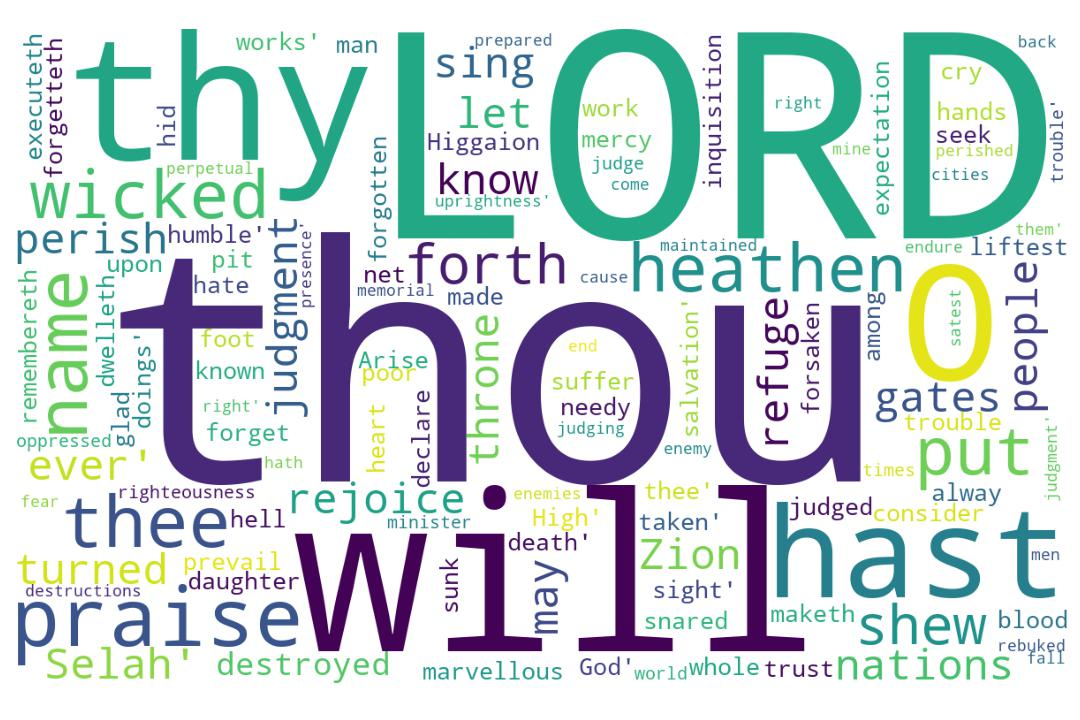
\includegraphics[width=\linewidth]{19OT-Psalms/Psalm9-WordCloud.jpg}
  \caption{Psalm 9 Word Cloud}
  \label{fig:Psalm 9 word Cloud}
\end{figure}

\marginpar{\scriptsize \centering \fcolorbox{bone}{lime}{\textbf{MANKIND AND HIS PLACE}}\\ (Psalm 9:1-20) \begin{compactenum}[I.][8]
    \item My \textbf{Rejoicing} \index[scripture]{Psalms!Psa 009:02}(Psa 9:2)
    \item God's \textbf{Rebuke} \index[scripture]{Psalms!Psa 009:05}(Psa 9:5)
    \item God's \textbf{Righteousness} \index[scripture]{Psalms!Psa 009:08}(Psa 9:8)
    \item God's \textbf{Remembrance} \index[scripture]{Psalms!Psa 009:12}(Psa 9:12)
    \item God's \textbf{Relief} \index[scripture]{Psalms!Psa 009:13}(Psa 9:13) (notably, a choice for man is available in verse 13.  Accept the mercy of God or perish in your own efforts to attain goodness)
    \item Human \textbf{Result} \index[scripture]{Psalms!Psa 009:15}(Psa 9:15) (mankind perishes in his own traps)
    \item Mankind's \textbf{Reality} \index[scripture]{Psalms!Psa 009:20}(Psa 9:20) (This is the Genesis 10 problem: man takes himself far too seriously. But he is just a human, made from  clay.)
    \item God's \textbf{Reminders} \index[scripture]{Psalms!Psa 009:20}(Psa 9:20) (It is God's mercy that reminds man of his place.)
\end{compactenum}}

\footnote{\textcolor[cmyk]{0.99998,1,0,0}{\hyperlink{TOC}{Return to end of Table of Contents.}}}\footnote{\href{https://audiobible.com/bible/bible.html}{\textcolor[cmyk]{0.99998,1,0,0}{Psalms Audio}}}\textcolor[cmyk]{0.99998,1,0,0}{To the chief Musician upon Muth-labben, A Psalm of David.}\\
\\
\textcolor[cmyk]{0.99998,1,0,0}{I will praise \emph{thee}, O LORD, with my whole heart; I will shew forth all thy marvellous works.}
[2] \textcolor[cmyk]{0.99998,1,0,0}{I will be glad and \fcolorbox{bone}{lime}{rejoice} in thee: I will sing praise to thy name, O thou most High.}
[3] \textcolor[cmyk]{0.99998,1,0,0}{When mine enemies are turned back, they shall fall and perish at thy presence.}
[4] \textcolor[cmyk]{0.99998,1,0,0}{For thou hast maintained my right and my cause; thou satest in the throne judging right.}
[5] \textcolor[cmyk]{0.99998,1,0,0}{Thou hast \fcolorbox{bone}{lime}{rebuked} the heathen, thou hast destroyed the wicked, thou hast put out their name for ever and ever.}
[6] \textcolor[cmyk]{0.99998,1,0,0}{O thou enemy, destructions are come to a perpetual end: and thou hast destroyed cities; their memorial is perished with them.}
[7] \textcolor[cmyk]{0.99998,1,0,0}{But the LORD shall endure for ever: he hath prepared his throne for judgment.}
[8] \textcolor[cmyk]{0.99998,1,0,0}{And he shall judge the world in \fcolorbox{bone}{lime}{righteousness}, he shall minister judgment to the people in uprightness.}
[9] \textcolor[cmyk]{0.99998,1,0,0}{The LORD also will be a refuge for the oppressed, a refuge in times of trouble.}
[10] \textcolor[cmyk]{0.99998,1,0,0}{And they that know thy name will put their trust in thee: for thou, LORD, hast not forsaken them that seek thee.}
[11] \textcolor[cmyk]{0.99998,1,0,0}{Sing praises to the LORD, which dwelleth in Zion: declare among the people his doings.}
[12] \textcolor[cmyk]{0.99998,1,0,0}{When he maketh inquisition for blood, he \fcolorbox{bone}{lime}{remembereth} them: he forgetteth not the cry of the humble.}
[13] \textcolor[cmyk]{0.99998,1,0,0}{Have mercy upon me, O LORD; consider my trouble \emph{which} \emph{I} \emph{suffer} of them that hate me, thou that liftest me up from the gates of death:}
[14] \textcolor[cmyk]{0.99998,1,0,0}{That I may shew forth all thy praise in the gates of the daughter of Zion: I will rejoice in thy salvation.}
[15] \textcolor[cmyk]{0.99998,1,0,0}{The heathen are sunk down in the pit \emph{that} they made: in \fcolorbox{bone}{lime}{the net which they hid} is their own foot taken.}
[16] \textcolor[cmyk]{0.99998,1,0,0}{The LORD is known \emph{by} the judgment \emph{which} he executeth: the wicked is snared in the work of his own hands. Higgaion. Selah.}
[17] \textcolor[cmyk]{0.99998,1,0,0}{The wicked shall be turned into hell, \emph{and} all the nations that forget God.}
[18] \textcolor[cmyk]{0.99998,1,0,0}{For the needy shall not alway be forgotten: the expectation of the poor shall \emph{not} perish for ever.}
[19] \textcolor[cmyk]{0.99998,1,0,0}{Arise, O LORD; \fcolorbox{bone}{lime}{let not man prevail}: let the heathen be judged in thy sight.}
[20] \textcolor[cmyk]{0.99998,1,0,0}{\fcolorbox{bone}{lime}{Put them in fear}, O LORD: \emph{that} the nations may know themselves \emph{to} \emph{be} \emph{but} men. Selah.}




\section{Psalm 9 Comments}


%\index[NWIV]{18!Psalms!Psa 9:1}\index[AWIP]{I!Psalms!Psa 9:1}\index[AWIP]{I!Psalms!Psa 9:1 (2)}\index[AWIP]{will!Psalms!Psa 9:1}\index[AWIP]{will!Psalms!Psa 9:1 (2)}\index[AWIP]{praise!Psalms!Psa 9:1}\index[AWIP]{\emph{thee}!Psalms!Psa 9:1}\index[AWIP]{O!Psalms!Psa 9:1}\index[AWIP]{LORD!Psalms!Psa 9:1}\index[AWIP]{with!Psalms!Psa 9:1}\index[AWIP]{my!Psalms!Psa 9:1}\index[AWIP]{whole!Psalms!Psa 9:1}\index[AWIP]{heart!Psalms!Psa 9:1}\index[AWIP]{shew!Psalms!Psa 9:1}\index[AWIP]{forth!Psalms!Psa 9:1}\index[AWIP]{all!Psalms!Psa 9:1}\index[AWIP]{thy!Psalms!Psa 9:1}\index[AWIP]{marvellous!Psalms!Psa 9:1}\index[AWIP]{works!Psalms!Psa 9:1}\index[AWIP]{\emph{thee}!Psalms!Psa 9:1}

\index[NWIV]{19!Psalms!Psa 9:2}\index[AWIP]{I!Psalms!Psa 9:2}\index[AWIP]{I!Psalms!Psa 9:2 (2)}\index[AWIP]{will!Psalms!Psa 9:2}\index[AWIP]{will!Psalms!Psa 9:2 (2)}\index[AWIP]{be!Psalms!Psa 9:2}\index[AWIP]{glad!Psalms!Psa 9:2}\index[AWIP]{and!Psalms!Psa 9:2}\index[AWIP]{rejoice!Psalms!Psa 9:2}\index[AWIP]{in!Psalms!Psa 9:2}\index[AWIP]{thee!Psalms!Psa 9:2}\index[AWIP]{sing!Psalms!Psa 9:2}\index[AWIP]{praise!Psalms!Psa 9:2}\index[AWIP]{to!Psalms!Psa 9:2}\index[AWIP]{thy!Psalms!Psa 9:2}\index[AWIP]{name!Psalms!Psa 9:2}\index[AWIP]{O!Psalms!Psa 9:2}\index[AWIP]{thou!Psalms!Psa 9:2}\index[AWIP]{most!Psalms!Psa 9:2}\index[AWIP]{High!Psalms!Psa 9:2}

\index[NWIV]{14!Psalms!Psa 9:3}\index[AWIP]{When!Psalms!Psa 9:3}\index[AWIP]{mine!Psalms!Psa 9:3}\index[AWIP]{enemies!Psalms!Psa 9:3}\index[AWIP]{are!Psalms!Psa 9:3}\index[AWIP]{turned!Psalms!Psa 9:3}\index[AWIP]{back!Psalms!Psa 9:3}\index[AWIP]{they!Psalms!Psa 9:3}\index[AWIP]{shall!Psalms!Psa 9:3}\index[AWIP]{fall!Psalms!Psa 9:3}\index[AWIP]{and!Psalms!Psa 9:3}\index[AWIP]{perish!Psalms!Psa 9:3}\index[AWIP]{at!Psalms!Psa 9:3}\index[AWIP]{thy!Psalms!Psa 9:3}\index[AWIP]{presence!Psalms!Psa 9:3}

\index[NWIV]{16!Psalms!Psa 9:4}\index[AWIP]{For!Psalms!Psa 9:4}\index[AWIP]{thou!Psalms!Psa 9:4}\index[AWIP]{thou!Psalms!Psa 9:4 (2)}\index[AWIP]{hast!Psalms!Psa 9:4}\index[AWIP]{maintained!Psalms!Psa 9:4}\index[AWIP]{my!Psalms!Psa 9:4}\index[AWIP]{my!Psalms!Psa 9:4 (2)}\index[AWIP]{right!Psalms!Psa 9:4}\index[AWIP]{right!Psalms!Psa 9:4 (2)}\index[AWIP]{and!Psalms!Psa 9:4}\index[AWIP]{cause!Psalms!Psa 9:4}\index[AWIP]{satest!Psalms!Psa 9:4}\index[AWIP]{in!Psalms!Psa 9:4}\index[AWIP]{the!Psalms!Psa 9:4}\index[AWIP]{throne!Psalms!Psa 9:4}\index[AWIP]{judging!Psalms!Psa 9:4}

\index[NWIV]{20!Psalms!Psa 9:5}\index[AWIP]{Thou!Psalms!Psa 9:5}\index[AWIP]{hast!Psalms!Psa 9:5}\index[AWIP]{hast!Psalms!Psa 9:5 (2)}\index[AWIP]{hast!Psalms!Psa 9:5 (3)}\index[AWIP]{rebuked!Psalms!Psa 9:5}\index[AWIP]{the!Psalms!Psa 9:5}\index[AWIP]{the!Psalms!Psa 9:5 (2)}\index[AWIP]{heathen!Psalms!Psa 9:5}\index[AWIP]{thou!Psalms!Psa 9:5}\index[AWIP]{thou!Psalms!Psa 9:5 (2)}\index[AWIP]{destroyed!Psalms!Psa 9:5}\index[AWIP]{wicked!Psalms!Psa 9:5}\index[AWIP]{put!Psalms!Psa 9:5}\index[AWIP]{out!Psalms!Psa 9:5}\index[AWIP]{their!Psalms!Psa 9:5}\index[AWIP]{name!Psalms!Psa 9:5}\index[AWIP]{for!Psalms!Psa 9:5}\index[AWIP]{ever!Psalms!Psa 9:5}\index[AWIP]{ever!Psalms!Psa 9:5 (2)}\index[AWIP]{and!Psalms!Psa 9:5}

\index[NWIV]{21!Psalms!Psa 9:6}\index[AWIP]{O!Psalms!Psa 9:6}\index[AWIP]{thou!Psalms!Psa 9:6}\index[AWIP]{thou!Psalms!Psa 9:6 (2)}\index[AWIP]{enemy!Psalms!Psa 9:6}\index[AWIP]{destructions!Psalms!Psa 9:6}\index[AWIP]{are!Psalms!Psa 9:6}\index[AWIP]{come!Psalms!Psa 9:6}\index[AWIP]{to!Psalms!Psa 9:6}\index[AWIP]{a!Psalms!Psa 9:6}\index[AWIP]{perpetual!Psalms!Psa 9:6}\index[AWIP]{end!Psalms!Psa 9:6}\index[AWIP]{and!Psalms!Psa 9:6}\index[AWIP]{hast!Psalms!Psa 9:6}\index[AWIP]{destroyed!Psalms!Psa 9:6}\index[AWIP]{cities!Psalms!Psa 9:6}\index[AWIP]{their!Psalms!Psa 9:6}\index[AWIP]{memorial!Psalms!Psa 9:6}\index[AWIP]{is!Psalms!Psa 9:6}\index[AWIP]{perished!Psalms!Psa 9:6}\index[AWIP]{with!Psalms!Psa 9:6}\index[AWIP]{them!Psalms!Psa 9:6}

\index[NWIV]{14!Psalms!Psa 9:7}\index[AWIP]{But!Psalms!Psa 9:7}\index[AWIP]{the!Psalms!Psa 9:7}\index[AWIP]{LORD!Psalms!Psa 9:7}\index[AWIP]{shall!Psalms!Psa 9:7}\index[AWIP]{endure!Psalms!Psa 9:7}\index[AWIP]{for!Psalms!Psa 9:7}\index[AWIP]{for!Psalms!Psa 9:7 (2)}\index[AWIP]{ever!Psalms!Psa 9:7}\index[AWIP]{he!Psalms!Psa 9:7}\index[AWIP]{hath!Psalms!Psa 9:7}\index[AWIP]{prepared!Psalms!Psa 9:7}\index[AWIP]{his!Psalms!Psa 9:7}\index[AWIP]{throne!Psalms!Psa 9:7}\index[AWIP]{judgment!Psalms!Psa 9:7}

\index[NWIV]{17!Psalms!Psa 9:8}\index[AWIP]{And!Psalms!Psa 9:8}\index[AWIP]{he!Psalms!Psa 9:8}\index[AWIP]{he!Psalms!Psa 9:8 (2)}\index[AWIP]{shall!Psalms!Psa 9:8}\index[AWIP]{shall!Psalms!Psa 9:8 (2)}\index[AWIP]{judge!Psalms!Psa 9:8}\index[AWIP]{the!Psalms!Psa 9:8}\index[AWIP]{the!Psalms!Psa 9:8 (2)}\index[AWIP]{world!Psalms!Psa 9:8}\index[AWIP]{in!Psalms!Psa 9:8}\index[AWIP]{in!Psalms!Psa 9:8 (2)}\index[AWIP]{righteousness!Psalms!Psa 9:8}\index[AWIP]{minister!Psalms!Psa 9:8}\index[AWIP]{judgment!Psalms!Psa 9:8}\index[AWIP]{to!Psalms!Psa 9:8}\index[AWIP]{people!Psalms!Psa 9:8}\index[AWIP]{uprightness!Psalms!Psa 9:8}

\index[NWIV]{16!Psalms!Psa 9:9}\index[AWIP]{The!Psalms!Psa 9:9}\index[AWIP]{LORD!Psalms!Psa 9:9}\index[AWIP]{also!Psalms!Psa 9:9}\index[AWIP]{will!Psalms!Psa 9:9}\index[AWIP]{be!Psalms!Psa 9:9}\index[AWIP]{a!Psalms!Psa 9:9}\index[AWIP]{a!Psalms!Psa 9:9 (2)}\index[AWIP]{refuge!Psalms!Psa 9:9}\index[AWIP]{refuge!Psalms!Psa 9:9 (2)}\index[AWIP]{for!Psalms!Psa 9:9}\index[AWIP]{the!Psalms!Psa 9:9}\index[AWIP]{oppressed!Psalms!Psa 9:9}\index[AWIP]{in!Psalms!Psa 9:9}\index[AWIP]{times!Psalms!Psa 9:9}\index[AWIP]{of!Psalms!Psa 9:9}\index[AWIP]{trouble!Psalms!Psa 9:9}

\index[NWIV]{22!Psalms!Psa 9:10}\index[AWIP]{And!Psalms!Psa 9:10}\index[AWIP]{they!Psalms!Psa 9:10}\index[AWIP]{that!Psalms!Psa 9:10}\index[AWIP]{that!Psalms!Psa 9:10 (2)}\index[AWIP]{know!Psalms!Psa 9:10}\index[AWIP]{thy!Psalms!Psa 9:10}\index[AWIP]{name!Psalms!Psa 9:10}\index[AWIP]{will!Psalms!Psa 9:10}\index[AWIP]{put!Psalms!Psa 9:10}\index[AWIP]{their!Psalms!Psa 9:10}\index[AWIP]{trust!Psalms!Psa 9:10}\index[AWIP]{in!Psalms!Psa 9:10}\index[AWIP]{thee!Psalms!Psa 9:10}\index[AWIP]{thee!Psalms!Psa 9:10 (2)}\index[AWIP]{for!Psalms!Psa 9:10}\index[AWIP]{thou!Psalms!Psa 9:10}\index[AWIP]{LORD!Psalms!Psa 9:10}\index[AWIP]{hast!Psalms!Psa 9:10}\index[AWIP]{not!Psalms!Psa 9:10}\index[AWIP]{forsaken!Psalms!Psa 9:10}\index[AWIP]{them!Psalms!Psa 9:10}\index[AWIP]{seek!Psalms!Psa 9:10}

\index[NWIV]{15!Psalms!Psa 9:11}\index[AWIP]{Sing!Psalms!Psa 9:11}\index[AWIP]{praises!Psalms!Psa 9:11}\index[AWIP]{to!Psalms!Psa 9:11}\index[AWIP]{the!Psalms!Psa 9:11}\index[AWIP]{the!Psalms!Psa 9:11 (2)}\index[AWIP]{LORD!Psalms!Psa 9:11}\index[AWIP]{which!Psalms!Psa 9:11}\index[AWIP]{dwelleth!Psalms!Psa 9:11}\index[AWIP]{in!Psalms!Psa 9:11}\index[AWIP]{Zion!Psalms!Psa 9:11}\index[AWIP]{declare!Psalms!Psa 9:11}\index[AWIP]{among!Psalms!Psa 9:11}\index[AWIP]{people!Psalms!Psa 9:11}\index[AWIP]{his!Psalms!Psa 9:11}\index[AWIP]{doings!Psalms!Psa 9:11}

\index[NWIV]{17!Psalms!Psa 9:12}\index[AWIP]{When!Psalms!Psa 9:12}\index[AWIP]{he!Psalms!Psa 9:12}\index[AWIP]{he!Psalms!Psa 9:12 (2)}\index[AWIP]{he!Psalms!Psa 9:12 (3)}\index[AWIP]{maketh!Psalms!Psa 9:12}\index[AWIP]{inquisition!Psalms!Psa 9:12}\index[AWIP]{for!Psalms!Psa 9:12}\index[AWIP]{blood!Psalms!Psa 9:12}\index[AWIP]{remembereth!Psalms!Psa 9:12}\index[AWIP]{them!Psalms!Psa 9:12}\index[AWIP]{forgetteth!Psalms!Psa 9:12}\index[AWIP]{not!Psalms!Psa 9:12}\index[AWIP]{the!Psalms!Psa 9:12}\index[AWIP]{the!Psalms!Psa 9:12 (2)}\index[AWIP]{cry!Psalms!Psa 9:12}\index[AWIP]{of!Psalms!Psa 9:12}\index[AWIP]{humble!Psalms!Psa 9:12}

\index[NWIV]{27!Psalms!Psa 9:13}\index[AWIP]{Have!Psalms!Psa 9:13}\index[AWIP]{mercy!Psalms!Psa 9:13}\index[AWIP]{upon!Psalms!Psa 9:13}\index[AWIP]{me!Psalms!Psa 9:13}\index[AWIP]{me!Psalms!Psa 9:13 (2)}\index[AWIP]{me!Psalms!Psa 9:13 (3)}\index[AWIP]{O!Psalms!Psa 9:13}\index[AWIP]{LORD!Psalms!Psa 9:13}\index[AWIP]{consider!Psalms!Psa 9:13}\index[AWIP]{my!Psalms!Psa 9:13}\index[AWIP]{trouble!Psalms!Psa 9:13}\index[AWIP]{\emph{which}!Psalms!Psa 9:13}\index[AWIP]{\emph{I}!Psalms!Psa 9:13}\index[AWIP]{\emph{suffer}!Psalms!Psa 9:13}\index[AWIP]{of!Psalms!Psa 9:13}\index[AWIP]{of!Psalms!Psa 9:13 (2)}\index[AWIP]{them!Psalms!Psa 9:13}\index[AWIP]{that!Psalms!Psa 9:13}\index[AWIP]{that!Psalms!Psa 9:13 (2)}\index[AWIP]{hate!Psalms!Psa 9:13}\index[AWIP]{thou!Psalms!Psa 9:13}\index[AWIP]{liftest!Psalms!Psa 9:13}\index[AWIP]{up!Psalms!Psa 9:13}\index[AWIP]{from!Psalms!Psa 9:13}\index[AWIP]{the!Psalms!Psa 9:13}\index[AWIP]{gates!Psalms!Psa 9:13}\index[AWIP]{death!Psalms!Psa 9:13}\index[AWIP]{\emph{which}!Psalms!Psa 9:13}\index[AWIP]{\emph{I}!Psalms!Psa 9:13}\index[AWIP]{\emph{suffer}!Psalms!Psa 9:13}

\index[NWIV]{22!Psalms!Psa 9:14}\index[AWIP]{That!Psalms!Psa 9:14}\index[AWIP]{I!Psalms!Psa 9:14}\index[AWIP]{I!Psalms!Psa 9:14 (2)}\index[AWIP]{may!Psalms!Psa 9:14}\index[AWIP]{shew!Psalms!Psa 9:14}\index[AWIP]{forth!Psalms!Psa 9:14}\index[AWIP]{all!Psalms!Psa 9:14}\index[AWIP]{thy!Psalms!Psa 9:14}\index[AWIP]{thy!Psalms!Psa 9:14 (2)}\index[AWIP]{praise!Psalms!Psa 9:14}\index[AWIP]{in!Psalms!Psa 9:14}\index[AWIP]{in!Psalms!Psa 9:14 (2)}\index[AWIP]{the!Psalms!Psa 9:14}\index[AWIP]{the!Psalms!Psa 9:14 (2)}\index[AWIP]{gates!Psalms!Psa 9:14}\index[AWIP]{of!Psalms!Psa 9:14}\index[AWIP]{of!Psalms!Psa 9:14 (2)}\index[AWIP]{daughter!Psalms!Psa 9:14}\index[AWIP]{Zion!Psalms!Psa 9:14}\index[AWIP]{will!Psalms!Psa 9:14}\index[AWIP]{rejoice!Psalms!Psa 9:14}\index[AWIP]{salvation!Psalms!Psa 9:14}

\index[NWIV]{22!Psalms!Psa 9:15}\index[AWIP]{The!Psalms!Psa 9:15}\index[AWIP]{heathen!Psalms!Psa 9:15}\index[AWIP]{are!Psalms!Psa 9:15}\index[AWIP]{sunk!Psalms!Psa 9:15}\index[AWIP]{down!Psalms!Psa 9:15}\index[AWIP]{in!Psalms!Psa 9:15}\index[AWIP]{in!Psalms!Psa 9:15 (2)}\index[AWIP]{the!Psalms!Psa 9:15}\index[AWIP]{the!Psalms!Psa 9:15 (2)}\index[AWIP]{pit!Psalms!Psa 9:15}\index[AWIP]{\emph{that}!Psalms!Psa 9:15}\index[AWIP]{they!Psalms!Psa 9:15}\index[AWIP]{they!Psalms!Psa 9:15 (2)}\index[AWIP]{made!Psalms!Psa 9:15}\index[AWIP]{net!Psalms!Psa 9:15}\index[AWIP]{which!Psalms!Psa 9:15}\index[AWIP]{hid!Psalms!Psa 9:15}\index[AWIP]{is!Psalms!Psa 9:15}\index[AWIP]{their!Psalms!Psa 9:15}\index[AWIP]{own!Psalms!Psa 9:15}\index[AWIP]{foot!Psalms!Psa 9:15}\index[AWIP]{taken!Psalms!Psa 9:15}\index[AWIP]{\emph{that}!Psalms!Psa 9:15}

\index[NWIV]{23!Psalms!Psa 9:16}\index[AWIP]{The!Psalms!Psa 9:16}\index[AWIP]{LORD!Psalms!Psa 9:16}\index[AWIP]{is!Psalms!Psa 9:16}\index[AWIP]{is!Psalms!Psa 9:16 (2)}\index[AWIP]{known!Psalms!Psa 9:16}\index[AWIP]{\emph{by}!Psalms!Psa 9:16}\index[AWIP]{the!Psalms!Psa 9:16}\index[AWIP]{the!Psalms!Psa 9:16 (2)}\index[AWIP]{the!Psalms!Psa 9:16 (3)}\index[AWIP]{judgment!Psalms!Psa 9:16}\index[AWIP]{\emph{which}!Psalms!Psa 9:16}\index[AWIP]{he!Psalms!Psa 9:16}\index[AWIP]{executeth!Psalms!Psa 9:16}\index[AWIP]{wicked!Psalms!Psa 9:16}\index[AWIP]{snared!Psalms!Psa 9:16}\index[AWIP]{in!Psalms!Psa 9:16}\index[AWIP]{work!Psalms!Psa 9:16}\index[AWIP]{of!Psalms!Psa 9:16}\index[AWIP]{his!Psalms!Psa 9:16}\index[AWIP]{own!Psalms!Psa 9:16}\index[AWIP]{hands!Psalms!Psa 9:16}\index[AWIP]{Higgaion!Psalms!Psa 9:16}\index[AWIP]{Selah!Psalms!Psa 9:16}\index[AWIP]{\emph{by}!Psalms!Psa 9:16}\index[AWIP]{\emph{which}!Psalms!Psa 9:16}

\index[NWIV]{14!Psalms!Psa 9:17}\index[AWIP]{The!Psalms!Psa 9:17}\index[AWIP]{wicked!Psalms!Psa 9:17}\index[AWIP]{shall!Psalms!Psa 9:17}\index[AWIP]{be!Psalms!Psa 9:17}\index[AWIP]{turned!Psalms!Psa 9:17}\index[AWIP]{into!Psalms!Psa 9:17}\index[AWIP]{hell!Psalms!Psa 9:17}\index[AWIP]{\emph{and}!Psalms!Psa 9:17}\index[AWIP]{all!Psalms!Psa 9:17}\index[AWIP]{the!Psalms!Psa 9:17}\index[AWIP]{nations!Psalms!Psa 9:17}\index[AWIP]{that!Psalms!Psa 9:17}\index[AWIP]{forget!Psalms!Psa 9:17}\index[AWIP]{God!Psalms!Psa 9:17}\index[AWIP]{\emph{and}!Psalms!Psa 9:17}

\index[NWIV]{18!Psalms!Psa 9:18}\index[AWIP]{For!Psalms!Psa 9:18}\index[AWIP]{the!Psalms!Psa 9:18}\index[AWIP]{the!Psalms!Psa 9:18 (2)}\index[AWIP]{the!Psalms!Psa 9:18 (3)}\index[AWIP]{needy!Psalms!Psa 9:18}\index[AWIP]{shall!Psalms!Psa 9:18}\index[AWIP]{shall!Psalms!Psa 9:18 (2)}\index[AWIP]{not!Psalms!Psa 9:18}\index[AWIP]{alway!Psalms!Psa 9:18}\index[AWIP]{be!Psalms!Psa 9:18}\index[AWIP]{forgotten!Psalms!Psa 9:18}\index[AWIP]{expectation!Psalms!Psa 9:18}\index[AWIP]{of!Psalms!Psa 9:18}\index[AWIP]{poor!Psalms!Psa 9:18}\index[AWIP]{\emph{not}!Psalms!Psa 9:18}\index[AWIP]{perish!Psalms!Psa 9:18}\index[AWIP]{for!Psalms!Psa 9:18}\index[AWIP]{ever!Psalms!Psa 9:18}\index[AWIP]{\emph{not}!Psalms!Psa 9:18}

\index[NWIV]{15!Psalms!Psa 9:19}\index[AWIP]{Arise!Psalms!Psa 9:19}\index[AWIP]{O!Psalms!Psa 9:19}\index[AWIP]{LORD!Psalms!Psa 9:19}\index[AWIP]{let!Psalms!Psa 9:19}\index[AWIP]{let!Psalms!Psa 9:19 (2)}\index[AWIP]{not!Psalms!Psa 9:19}\index[AWIP]{man!Psalms!Psa 9:19}\index[AWIP]{prevail!Psalms!Psa 9:19}\index[AWIP]{the!Psalms!Psa 9:19}\index[AWIP]{heathen!Psalms!Psa 9:19}\index[AWIP]{be!Psalms!Psa 9:19}\index[AWIP]{judged!Psalms!Psa 9:19}\index[AWIP]{in!Psalms!Psa 9:19}\index[AWIP]{thy!Psalms!Psa 9:19}\index[AWIP]{sight!Psalms!Psa 9:19}

\index[NWIV]{17!Psalms!Psa 9:20}\index[AWIP]{Put!Psalms!Psa 9:20}\index[AWIP]{them!Psalms!Psa 9:20}\index[AWIP]{in!Psalms!Psa 9:20}\index[AWIP]{fear!Psalms!Psa 9:20}\index[AWIP]{O!Psalms!Psa 9:20}\index[AWIP]{LORD!Psalms!Psa 9:20}\index[AWIP]{\emph{that}!Psalms!Psa 9:20}\index[AWIP]{the!Psalms!Psa 9:20}\index[AWIP]{nations!Psalms!Psa 9:20}\index[AWIP]{may!Psalms!Psa 9:20}\index[AWIP]{know!Psalms!Psa 9:20}\index[AWIP]{themselves!Psalms!Psa 9:20}\index[AWIP]{\emph{to}!Psalms!Psa 9:20}\index[AWIP]{\emph{be}!Psalms!Psa 9:20}\index[AWIP]{\emph{but}!Psalms!Psa 9:20}\index[AWIP]{men!Psalms!Psa 9:20}\index[AWIP]{Selah!Psalms!Psa 9:20}\index[AWIP]{\emph{that}!Psalms!Psa 9:20}\index[AWIP]{\emph{to}!Psalms!Psa 9:20}\index[AWIP]{\emph{be}!Psalms!Psa 9:20}\index[AWIP]{\emph{but}!Psalms!Psa 9:20}


\section{Psalm 9 Outlines}

\subsection{My Outlines}

\subsubsection{Mankind and his Place}

\index[speaker]{Keith Anthony!Psalm 009 (Mankind and his Place)}
\index[series]{Psalms (Keith Anthony)!Psalm 009 (Mankind and his Place)}
\index[date]{2017/01/09!Psalm 009 (Mankind and his Place) (Keith Anthony)}

\begin{compactenum}[I.]
    \item My \textbf{Rejoicing} \index[scripture]{Psalms!Psa 009:02}(Psa 9:2)
    \item God's \textbf{Rebuke} \index[scripture]{Psalms!Psa 009:05}(Psa 9:5)
    \item God's \textbf{Righteousness} \index[scripture]{Psalms!Psa 009:08}(Psa 9:8)
    \item God's \textbf{Remembrance} \index[scripture]{Psalms!Psa 009:12}(Psa 9:12)
    \item God's \textbf{Relief} \index[scripture]{Psalms!Psa 009:13}(Psa 9:13) (notably, a choice for man is available in verse 13.  Accept the mercy of God or perish in your own efforts to attain goodness)
    \item Human \textbf{Result} \index[scripture]{Psalms!Psa 009:15}(Psa 9:15) (mankind perishes in his own traps)
    \item Mankind's \textbf{Reality} \index[scripture]{Psalms!Psa 009:20}(Psa 9:20) (This is the Genesis 10 problem: man takes himself far too seriously. But he is just a human, made from  clay.)
    \item God's \textbf{Reminders} \index[scripture]{Psalms!Psa 009:20}(Psa 9:20) (It is God's mercy that reminds man of his place.)
\end{compactenum}


\subsection{Outlines from Others}

\subsubsection{Let's Just Praise the Lord}
Psalm 9:
\index[speaker]{unknown!Psalm 009 (Let's Just Praise the Lord)}
\index[series]{Psalms (unknown)!Psalm 009 (Let's Just Praise the Lord)}
\index[date]{unknown!Psalm 009 (Let's Just Praise the Lord) (unknown)}
% original {0.12, 0.3, 0.17},  forestgreen

\begin{compactenum}[I.][3]
    \item The Completeness of Praise \index[scripture]{Psalms!Psa 009:01}(Psalm 9:1)
    \begin{compactenum}[A.]
        \item ``$\hdots$ with my whole heart $\hdots$''
        \item ``$\hdots$ all thy marvelous works $\hdots$ ''
    \end{compactenum}
    \item The Concert of Praise \index[scripture]{Psalms!Psa 009:02}(Psalm 9:2)
    \begin{compactenum}[A.]
        \item ``$\hdots$ I will be glad and rejoice  $\hdots$''
        \item ``$\hdots$ I will sing praise to thy name $\hdots$ ''
    \end{compactenum}
    \item The Causes of Praise \index[scripture]{Psalms!Psa 009:03-04}(Psalm 9:3--4)
    \begin{compactenum}[A.]
        \item ``When my enemies are turned back, they shall fall and perish at thy presence.'' 
        \item `For thou hast maintained my right and my cause $\hdots$ ''
    \end{compactenum}
\end{compactenum} 


%\section{Psalm 9 Statistics}

%%%%%%%%%%%%%%%%%%%%%%%%%%%
%%%%% Word Statistics
%%%%%%%%%%%%%%%%%%%%%%%%%%


\normalsize



\subsection{Chapter Word Statistics}


%%%%%%%%%%
%%%%%%%%%%
 
\begin{center}
\begin{longtable}{l|c|c|c|c}
\caption[Stats for Psalm 9]{Stats for Psalm 9} \label{table:Stats for Psalm 9} \\ 
\hline \multicolumn{1}{|c|}{\textbf{Verse(s)}} & \multicolumn{1}{|c|}{\textbf{Count}} & \multicolumn{1}{|c|}{\textbf{Unique}} & \multicolumn{1}{|c|}{\textbf{Italics}} & \multicolumn{1}{|c|}{\textbf{Uniq Italic}}  \\ \hline 
\endfirsthead
 
\multicolumn{5}{c}
{{\bfseries \tablename\ \thetable{} -- continued from previous page}} \\  
\hline \multicolumn{1}{|c|}{\textbf{Verse(s)}} & \multicolumn{1}{|c|}{\textbf{Count}} & \multicolumn{1}{|c|}{\textbf{Unique}} & \multicolumn{1}{|c|}{\textbf{Italics}} & \multicolumn{1}{|c|}{\textbf{Uniq Italic}}  \\ \hline 
\endhead
 
\hline \multicolumn{5}{|r|}{{Continued if needed}} \\ \hline
\endfoot 
1 & 18 & 9 & 0 & 0\\ \hline
2 & 0 & 9 & 0 & 0\\ \hline
3 & 0 & 9 & 0 & 0\\ \hline
4 & 0 & 9 & 0 & 0\\ \hline
5 & 0 & 9 & 0 & 0\\ \hline
6 & 0 & 9 & 0 & 0\\ \hline
7 & 0 & 9 & 0 & 0\\ \hline
8 & 0 & 9 & 0 & 0\\ \hline
9 & 0 & 9 & 0 & 0\\ \hline
10 & 0 & 9 & 0 & 0\\ \hline
\hline \hline
Total & 534 & 231 & 16 & 14



\end{longtable}
\end{center}

%%%%%%%%%%
%%%%%%%%%%
 
\subsection{Words by Frequency}

\begin{center}
\begin{longtable}{l|r}
\caption[Word Frequencies in Psalm 109]{Word Frequencies in Psalm 109} \label{table:WordsIn-Psalm-109} \\ 
\hline \multicolumn{1}{|c|}{\textbf{Word}} & \multicolumn{1}{c|}{\textbf{Frequency}} \\ \hline 
\endfirsthead
 
\multicolumn{2}{c}
{{\bfseries \tablename\ \thetable{} -- continued from previous page}} \\ 
\hline \multicolumn{1}{|c|}{\textbf{Word}} & \multicolumn{1}{c|}{\textbf{Frequency}} \\ \hline 
\endhead
 
\hline \multicolumn{2}{|r|}{{Continued if needed}} \\ \hline
\endfoot
 
\hline \hline
\endlastfoot
the & 25 \\ \hline

those & 1 \\ \hline
condemn & 1 \\ \hline
\end{longtable}
\end{center}



\normalsize



\subsection{Words Alphabetically}

\begin{center}
\begin{longtable}{l|r}
\caption[Word Alphabetically in Psalm 9]{Word Alphabetically in Psalm 9} \label{table:WordsIn-Psalm-9} \\ 
\hline \multicolumn{1}{|c|}{\textbf{Word}} & \multicolumn{1}{c|}{\textbf{Frequency}} \\ \hline 
\endfirsthead
 
\multicolumn{2}{c}
{{\bfseries \tablename\ \thetable{} -- continued from previous page}} \\ 
\hline \multicolumn{1}{|c|}{\textbf{Word}} & \multicolumn{1}{c|}{\textbf{Frequency}} \\ \hline 
\endhead
 
\hline \multicolumn{2}{|r|}{{Continued if needed}} \\ \hline
\endfoot
 
\hline \hline
\endlastfoot
And & 1 \\ \hline
As & 2 \\ \hline
Because & 1 \\ \hline
But & 1 \\ \hline
For & 4 \\ \hline
GOD & 1 \\ \hline
God & 2 \\ \hline
Help & 1 \\ \hline
Hold & 1 \\ \hline
I & 7 \\ \hline
LORD & 6 \\ \hline
Let & 11 \\ \hline
Lord & 1 \\ \hline
My & 1 \\ \hline
O & 4 \\ \hline
Satan & 1 \\ \hline
Set & 1 \\ \hline
That & 1 \\ \hline
They & 1 \\ \hline
When & 1 \\ \hline
\emph{Let} & 1 \\ \hline
\emph{am} & 1 \\ \hline
\emph{and} & 2 \\ \hline
\emph{be} & 1 \\ \hline
\emph{bread} & 1 \\ \hline
\emph{give} & 1 \\ \hline
\emph{him} & 1 \\ \hline
\emph{is} & 2 \\ \hline
\emph{myself} & 1 \\ \hline
\emph{that} & 1 \\ \hline
\emph{their} & 1 \\ \hline
\emph{unto} & 1 \\ \hline
\emph{when} & 1 \\ \hline
\emph{which} & 1 \\ \hline
a & 7 \\ \hline
about & 1 \\ \hline
according & 1 \\ \hline
adversaries & 3 \\ \hline
against & 4 \\ \hline
all & 1 \\ \hline
also & 3 \\ \hline
am & 2 \\ \hline
among & 1 \\ \hline
and & 18 \\ \hline
another & 1 \\ \hline
any & 1 \\ \hline
are & 3 \\ \hline
arise & 1 \\ \hline
as & 5 \\ \hline
ashamed & 1 \\ \hline
at & 2 \\ \hline
be & 16 \\ \hline
became & 1 \\ \hline
because & 1 \\ \hline
become & 1 \\ \hline
before & 1 \\ \hline
beg & 1 \\ \hline
bless & 1 \\ \hline
blessing & 1 \\ \hline
blotted & 2 \\ \hline
bones & 1 \\ \hline
bowels & 1 \\ \hline
broken & 1 \\ \hline
but & 4 \\ \hline
catch & 1 \\ \hline
cause & 1 \\ \hline
children & 3 \\ \hline
clothed & 2 \\ \hline
come & 2 \\ \hline
compassed & 1 \\ \hline
condemn & 1 \\ \hline
condemned & 1 \\ \hline
confusion & 1 \\ \hline
continually & 3 \\ \hline
cover & 1 \\ \hline
covereth & 1 \\ \hline
curse & 1 \\ \hline
cursing & 2 \\ \hline
cut & 2 \\ \hline
days & 1 \\ \hline
deceitful & 1 \\ \hline
declineth & 1 \\ \hline
delighted & 1 \\ \hline
deliver & 1 \\ \hline
desolate & 1 \\ \hline
do & 1 \\ \hline
done & 1 \\ \hline
down & 1 \\ \hline
earth & 1 \\ \hline
even & 1 \\ \hline
evil & 2 \\ \hline
extend & 1 \\ \hline
extortioner & 1 \\ \hline
faileth & 1 \\ \hline
far & 1 \\ \hline
fasting & 1 \\ \hline
fatherless & 2 \\ \hline
fathers & 1 \\ \hline
fatness & 1 \\ \hline
favour & 1 \\ \hline
few & 1 \\ \hline
flesh & 1 \\ \hline
following & 1 \\ \hline
for & 5 \\ \hline
fought & 1 \\ \hline
from & 4 \\ \hline
garment & 2 \\ \hline
generation & 1 \\ \hline
girded & 1 \\ \hline
girdle & 1 \\ \hline
gone & 1 \\ \hline
good & 2 \\ \hline
greatly & 1 \\ \hline
hand & 3 \\ \hline
hast & 1 \\ \hline
hath & 1 \\ \hline
hatred & 2 \\ \hline
have & 2 \\ \hline
he & 10 \\ \hline
heads & 1 \\ \hline
heart & 2 \\ \hline
him & 8 \\ \hline
himself & 1 \\ \hline
his & 16 \\ \hline
in & 3 \\ \hline
iniquity & 1 \\ \hline
into & 2 \\ \hline
is & 2 \\ \hline
it & 6 \\ \hline
judged & 1 \\ \hline
knees & 1 \\ \hline
know & 1 \\ \hline
labour & 1 \\ \hline
let & 15 \\ \hline
like & 4 \\ \hline
locust & 1 \\ \hline
looked & 1 \\ \hline
love & 2 \\ \hline
loved & 1 \\ \hline
lying & 1 \\ \hline
man & 2 \\ \hline
mantle & 1 \\ \hline
may & 2 \\ \hline
me & 11 \\ \hline
memory & 1 \\ \hline
mercy & 4 \\ \hline
might & 1 \\ \hline
mine & 2 \\ \hline
mother & 1 \\ \hline
mouth & 3 \\ \hline
multitude & 1 \\ \hline
my & 9 \\ \hline
name & 1 \\ \hline
name's & 1 \\ \hline
needy & 2 \\ \hline
neither & 1 \\ \hline
none & 1 \\ \hline
not & 4 \\ \hline
of & 12 \\ \hline
off & 2 \\ \hline
office & 1 \\ \hline
oil & 1 \\ \hline
opened & 1 \\ \hline
out & 3 \\ \hline
over & 1 \\ \hline
own & 1 \\ \hline
peace & 1 \\ \hline
persecuted & 1 \\ \hline
places & 1 \\ \hline
poor & 3 \\ \hline
posterity & 1 \\ \hline
praise & 3 \\ \hline
prayer & 2 \\ \hline
rejoice & 1 \\ \hline
remembered & 2 \\ \hline
reproach & 1 \\ \hline
reward & 1 \\ \hline
rewarded & 1 \\ \hline
right & 2 \\ \hline
sake & 1 \\ \hline
save & 2 \\ \hline
seek & 1 \\ \hline
servant & 1 \\ \hline
shadow & 1 \\ \hline
shaked & 1 \\ \hline
shall & 2 \\ \hline
shame & 1 \\ \hline
shew & 1 \\ \hline
sin & 2 \\ \hline
slay & 1 \\ \hline
so & 3 \\ \hline
soul & 2 \\ \hline
speak & 1 \\ \hline
spoil & 1 \\ \hline
spoken & 1 \\ \hline
stand & 2 \\ \hline
strangers & 1 \\ \hline
take & 1 \\ \hline
that & 7 \\ \hline
the & 25 \\ \hline
their & 4 \\ \hline
them & 8 \\ \hline
themselves & 1 \\ \hline
there & 2 \\ \hline
they & 7 \\ \hline
this & 2 \\ \hline
those & 1 \\ \hline
thou & 5 \\ \hline
through & 1 \\ \hline
thy & 6 \\ \hline
to & 5 \\ \hline
tongue & 1 \\ \hline
tossed & 1 \\ \hline
unto & 4 \\ \hline
up & 1 \\ \hline
upon & 1 \\ \hline
vagabonds & 1 \\ \hline
water & 1 \\ \hline
weak & 1 \\ \hline
when & 2 \\ \hline
wherewith & 1 \\ \hline
wicked & 2 \\ \hline
widow & 1 \\ \hline
wife & 1 \\ \hline
will & 2 \\ \hline
with & 9 \\ \hline
within & 1 \\ \hline
without & 1 \\ \hline
words & 1 \\ \hline
wounded & 1 \\ \hline
yea & 1 \\ \hline
\end{longtable}
\end{center}



\normalsize



\subsection{Word Lengths in Chapter}
\normalsize
\begin{longtable}{l|p{3.75in}}
\caption[Words by Length in Psalm 9]{Words by Length in Psalm 9} \label{table:WordsIn-Psalm-9} \\ 
\hline \multicolumn{1}{|c|}{\textbf{Length}} & \multicolumn{1}{c|}{\textbf{Words}} \\ \hline 
\endfirsthead
 
\multicolumn{2}{c}
{{\bfseries \tablename\ \thetable{} -- continued from previous page}} \\ 
\hline \multicolumn{1}{|c|}{\textbf{Length}} & \multicolumn{1}{c|}{\textbf{Words}} \\ \hline 
\endhead
 
\hline \multicolumn{2}{|r|}{{Continued if needed}} \\ \hline
\endfoot
 
\hline \hline
\endlastfoot
1 & O, a, I \\ \hline
2 & of, my, me, at, he, be, to, in, As, so, it, as, is, \emph{be}, do, \emph{is}, \emph{am}, am, up, My \\ \hline
3 & not, thy, God, For, the, and, are, but, And, for, Set, man, him, let, his, sin, Let, few, \emph{and}, beg, out, all, any, cut, off, may, far, oil, \emph{Let}, But, GOD, own, yea, \emph{him} \\ \hline
4 & Hold, they, have, with, They, also, love, \emph{give}, \emph{unto}, evil, good, thou, over, hand, When, days, take, wife, them, seek, that, hath, none, unto, name, LORD, from, shew, poor, even, slay, come, like, into, this, mine, soul, Lord, sake, gone, when, down, weak, \emph{when}, upon, Help, save, That, know, \emph{that}, hast, done, will \\ \hline
5 & peace, mouth, lying, about, words, cause, Satan, stand, right, shall, widow, \emph{their}, \emph{bread}, their, catch, spoil, there, mercy, earth, needy, might, heart, loved, water, bones, \emph{which}, speak, knees, flesh, heads, curse, bless, arise, shame, cover, among, those \\ \hline
6 & praise, wicked, opened, spoken, tongue, hatred, fought, \emph{myself}, prayer, judged, become, office, places, labour, extend, favour, mother, before, memory, broken, bowels, girdle, girded, reward, name's, within, shadow, tossed, locust, became, looked, shaked, mantle \\ \hline
7 & against, without, another, neither, blotted, fathers, Because, cursing, clothed, himself, garment, because, deliver, wounded, through, fasting, faileth, fatness, ashamed, servant, rejoice, greatly, condemn \\ \hline
8 & rewarded, children, desolate, iniquity, blessing, covereth, reproach \\ \hline
9 & deceitful, compassed, condemned, vagabonds, strangers, posterity, following, delighted, wherewith, declineth, according, confusion, multitude \\ \hline
10 & fatherless, generation, remembered, persecuted, themselves \\ \hline
11 & adversaries, continually, extortioner \\ \hline
\end{longtable}






%%%%%%%%%%
%%%%%%%%%%
 



%%%%%%%%%%
%%%%%%%%%%
\subsection{Verses with 13 Words in Chapter}
\normalsize
\begin{longtable}{l|p{3.75in}}
\caption[Verses with 13 Words  in Psalm 9]{Verses with 13 Words  in Psalm 9} \label{table:Verses with 13 Words in-Psalm-9} \\ 
\hline \multicolumn{1}{|c|}{\textbf{Reference}} & \multicolumn{1}{c|}{\textbf{Verse}} \\ \hline 
\endfirsthead
 
\multicolumn{2}{c}
{{\bfseries \tablename\ \thetable{} -- continued from previous page}} \\ 
\hline \multicolumn{1}{|c|}{\textbf{Reference}} & \multicolumn{1}{c|}{\textbf{Verse}} \\ \hline 
\endhead
 
\hline \multicolumn{2}{|r|}{{Continued if needed}} \\ \hline
\endfoot
 
\hline \hline
\endlastfoot
Psalms 109:4 & For my love they are my adversaries: but I \emph{give} \emph{myself} \emph{unto} prayer. \\ \hline
Psalms 109:5 & And they have rewarded me evil for good, and hatred for my love. \\ \hline
Psalms 109:22 & For I \emph{am} poor and needy, and my heart is wounded within me. \\ \hline
Psalms 109:26 & Help me, O LORD my God: O save me according to thy mercy: \\ \hline
\end{longtable}






%%%%%%%%%%
%%%%%%%%%%
 



%%%%%%%%%%
%%%%%%%%%%
\subsection{Verses with 18 Words in Chapter}
\normalsize
\begin{longtable}{l|p{3.75in}}
\caption[Verses with 18 Words  in Psalm 9]{Verses with 18 Words  in Psalm 9} \label{table:Verses with 18 Words in-Psalm-9} \\ 
\hline \multicolumn{1}{|c|}{\textbf{Reference}} & \multicolumn{1}{c|}{\textbf{Verse}} \\ \hline 
\endfirsthead
 
\multicolumn{2}{c}
{{\bfseries \tablename\ \thetable{} -- continued from previous page}} \\ 
\hline \multicolumn{1}{|c|}{\textbf{Reference}} & \multicolumn{1}{c|}{\textbf{Verse}} \\ \hline 
\endhead
 
\hline \multicolumn{2}{|r|}{{Continued if needed}} \\ \hline
\endfoot
 
\hline \hline
\endlastfoot
Psalms 109:23 & I am gone like the shadow when it declineth: I am tossed up and down as the locust. \\ \hline
Psalms 109:28 & Let them curse, but bless thou: when they arise, let them be ashamed; but let thy servant rejoice. \\ \hline
\end{longtable}






%%%%%%%%%%
%%%%%%%%%%
\subsection{Psalm 9 Repeated Phrases}


%%%%%%%%%%
%%%%%%%%%%
\normalsize
 
\begin{center}
\begin{longtable}{|p{3.0in}|p{0.5in}|}
\caption[Psalm 9 Repeated Phrases]{Psalm 9 Repeated Phrases}\label{table:Repeated Phrases Psalm 9} \\
\hline \multicolumn{1}{|c|}{\textbf{Phrase}} & \multicolumn{1}{c|}{\textbf{Frequency}} \\ \hline 
\endfirsthead
 
\multicolumn{2}{c}
{{\bfseries \tablename\ \thetable{} -- continued from previous page}} \\  
\hline \multicolumn{1}{|c|}{\textbf{Phrase}} & \multicolumn{1}{c|}{\textbf{Frequency}} \\ \hline 
\endhead
 
\hline \multicolumn{2}{c}{{ }} \\ \hline
\endfoot 
I will & 5\\ \hline 
in the & 5\\ \hline 
O LORD & 4\\ \hline 
thou hast & 4\\ \hline 
for ever & 3\\ \hline 
of the & 3\\ \hline 
\end{longtable}
\end{center}



%%%%%%%%%%
%%%%%%%%%%




% COLORED HIGHLIGHT BEX -- \fcolorbox{bone}{lime}{Abib}
\chapter{Psalm 10}

\begin{figure}
  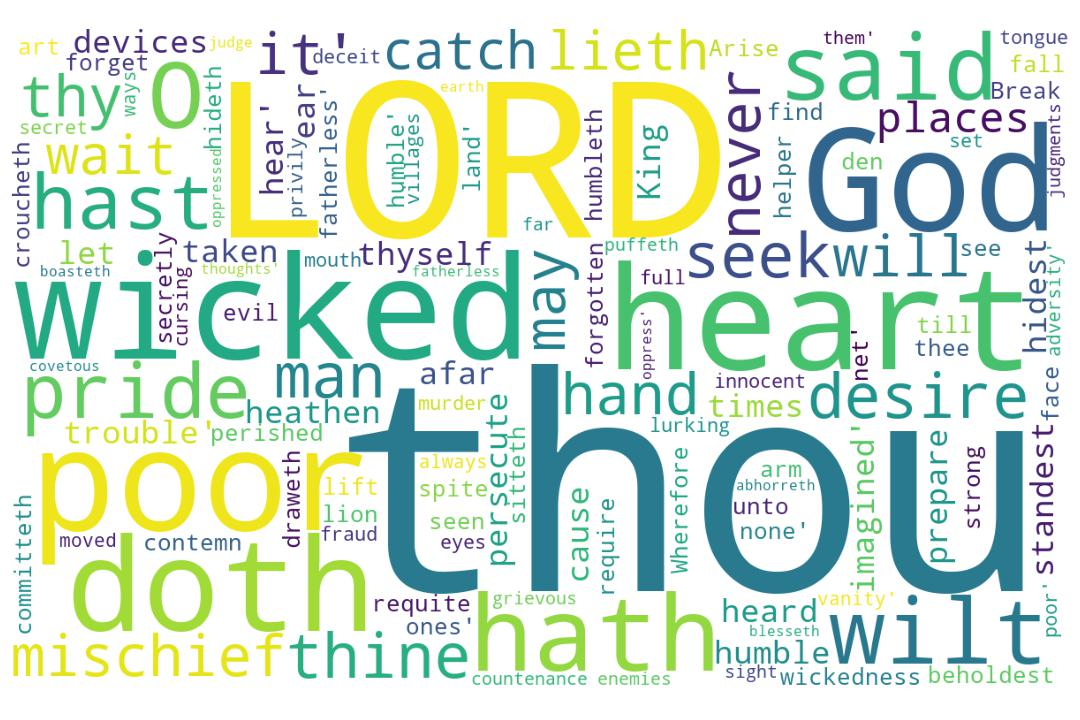
\includegraphics[width=\linewidth]{19OT-Psalms/Psalm10-WordCloud.jpg}
  \caption{Psalm 10 Word Cloud}
  \label{fig:Psalm 10 word Cloud}
\end{figure}


\marginpar{\scriptsize \centering \fcolorbox{bone}{lime}{\textbf{WHEN GOD SEEMS FAR AWAY}}\\ (Psalm 10:1-18)
\begin{compactenum}[I.][8]
    \item The \textbf{Evil Person} (Wicked) \index[scripture]{Psalms!Psa 010:02}\index[scripture]{Psalms!Psa 010:03}\index[scripture]{Psalms!Psa 010:04}\index[scripture]{Psalms!Psa 010:13}\index[scripture]{Psalms!Psa 010:15}(Psa 10:2, 3, 4, 13, 15) 
    \begin{compactenum}[A.]
	\item He persecutes \index[scripture]{Psalms!Psa 010:02}(Psa 10:2) 
    	\item He boasts \index[scripture]{Psalms!Psa 010:03}(Psa 10:3) 
   	\item He ignores God \index[scripture]{Psalms!Psa 010:04}(Psa 10:4) 
    	\item He curses \index[scripture]{Psalms!Psa 010:0}(Psa 10:7) 
    	\item He ambushes \index[scripture]{Psalms!Psa 010:08}(Psa 10:8) 
    	\item He Acts vindicated \index[scripture]{Psalms!Psa 010:11}(Psa 10:11) 
    \end{compactenum}
    \item An \textbf{Earnest Prayer} (Waiting) \index[scripture]{Psalms!Psa 010:12}(Psa 10:12) 
    \item An \textbf{Extended Preparation} (Withstand) \index[scripture]{Psalms!Psa 010:17}(Psa 10:17) 
    \item The \textbf{Enduring Promise} (Win) \index[scripture]{Psalms!Psa 010:18}(Psa 10:18) 
\end{compactenum}}


\marginpar{\scriptsize \centering \fcolorbox{bone}{yellow}{\textbf{10 MINUTES OF FAME}}\\ (Psalm 10:1-18)
\begin{compactenum}[I.][8]
    \item The \textbf{Strange Silence} \index[scripture]{Psalms!Psa 010:01}(Psa 10:1) 
    \item \textbf{Successful Sin} \index[scripture]{Psalms!Psa 010:02}(Psa 10:2) 
    \item \textbf{Scorning Statements Sin} \index[scripture]{Psalms!Psa 010:03}(Psa 10:3) 
    \item \textbf{Secret Seductions} \index[scripture]{Psalms!Psa 010:09}(Psa 10:9) 
    \item \textbf{Spiteful Speech} \index[scripture]{Psalms!Psa 010:13}(Psa 10:13) 
    \item The \textbf{Sweeping Slaughter} \index[scripture]{Psalms!Psa 010:15}(Psa 10:15) 
    \item A \textbf{Sovereign Supremacy} \index[scripture]{Psalms!Psa 010:16}(Psa 10:16) 
\end{compactenum}}

\footnote{\textcolor[cmyk]{0.99998,1,0,0}{\hyperlink{TOC}{Return to end of Table of Contents.}}}\footnote{\href{https://audiobible.com/bible/genesis_30.html}{\textcolor[cmyk]{0.99998,1,0,0}{Psalms Audio}}}\textcolor[cmyk]{0.99998,1,0,0}{Why\textcolor{jungle}{$_{2066}^{1}$} standest thou afar off, O LORD? \emph{why} hidest thou \emph{thyself} \underline{in} times of trouble?}\footnote{\textbf{Psalm 9:9} - The LORD also will be a refuge for the oppressed, a refuge in times of trouble.}
[2] \textcolor[cmyk]{0.99998,1,0,0}{The\textcolor{jungle}{$_{2081}^{16}$} \fcolorbox{bone}{lime}{wicked} \underline{in} \emph{his} pride doth persecute the poor: let them be taken \underline{in} the devices that they have imagined.}\footnote{\textbf{Job 41:34} - He beholdeth all high things: he is a king over all the children of pride.}
[3] \textcolor[cmyk]{0.99998,1,0,0}{For\textcolor{jungle}{$_{2101}^{36}$} the \fcolorbox{bone}{lime}{wicked} boasteth of his heart's desire, and blesseth the covetous, \emph{whom} the LORD abhorreth.}
[4] \textcolor[cmyk]{0.99998,1,0,0}{The\textcolor{jungle}{$_{2117}^{52}$} \fcolorbox{bone}{lime}{wicked}, through the pride of his countenance, will not seek \emph{after} \emph{God}: God \emph{is} not \underline{in} all his thoughts.}
[5] \textcolor[cmyk]{0.99998,1,0,0}{His\textcolor{jungle}{$_{2137}^{72}$} ways are always grievous; thy judgments \emph{are} far above out of his sight: \emph{as} \emph{for} all his enemies, he puffeth at them.}
[6] \textcolor[cmyk]{0.99998,1,0,0}{He\textcolor{jungle}{$_{2160}^{95}$} hath said \underline{in} his heart, I shall not be moved: for \emph{I} \emph{shall} never \emph{be} \underline{in} adversity.}
[7] \textcolor[cmyk]{0.99998,1,0,0}{His\textcolor{jungle}{$_{2178}^{113}$} mouth is full of cursing and deceit and fraud: under his tongue \emph{is} mischief and vanity.}
[8] \textcolor[cmyk]{0.99998,1,0,0}{He\textcolor{jungle}{$_{2195}^{130}$} sitteth \underline{in} the lurking places of the villages: \underline{in} the secret places doth he murder the innocent: his eyes are privily set against the poor.}
[9] \textcolor[cmyk]{0.99998,1,0,0}{He\textcolor{jungle}{$_{2221}^{156}$} lieth \underline{in} wait secretly as a lion \underline{in} his den: he lieth \underline{in} wait to catch the poor: he doth catch the poor, when he draweth him into his net.}\footnote{\textbf{1 Peter 5:8} - Be sober, be vigilant; because your adversary the devil, as a roaring lion, walketh about, seeking whom he may devour:}
[10] \textcolor[cmyk]{0.99998,1,0,0}{He\textcolor{jungle}{$_{2252}^{187}$} croucheth, \emph{and} humbleth himself, that the poor may fall by his strong ones.}
[11] \textcolor[cmyk]{0.99998,1,0,0}{He\textcolor{jungle}{$_{2266}^{201}$} hath said \underline{in} his heart, God hath forgotten: he hideth his face; he will never see \emph{it}.}
[12] \textcolor[cmyk]{0.99998,1,0,0}{Arise\textcolor{jungle}{$_{2284}^{219}$}, O LORD; O God, lift up thine hand: \fcolorbox{bone}{lime}{forget not the humble}.}
[13] \textcolor[cmyk]{0.99998,1,0,0}{Wherefore\textcolor{jungle}{$_{2297}^{232}$} doth the \fcolorbox{bone}{lime}{wicked} contemn God? he hath said \underline{in} his heart, Thou wilt not require \emph{it}.}
[14] \textcolor[cmyk]{0.99998,1,0,0}{Thou\textcolor{jungle}{$_{2314}^{249}$} hast seen \emph{it}; for thou beholdest mischief and spite, to requite \emph{it} with thy hand: the poor committeth himself unto thee; thou art the helper of the fatherless.}
[15] \textcolor[cmyk]{0.99998,1,0,0}{Break\textcolor{jungle}{$_{2343}^{278}$} thou the arm of the \fcolorbox{bone}{lime}{wicked} and the evil \emph{man}: seek out his wickedness \emph{till} thou find none.}\footnote{\textbf{Zechariah 11:17} -  Woe to the idol shepherd that leaveth the flock! the sword shall be upon his arm, and upon his right eye: his arm shall be clean dried up, and his right eye shall be utterly darkened.}
[16] \textcolor[cmyk]{0.99998,1,0,0}{The\textcolor{jungle}{$_{2362}^{297}$} LORD \emph{is} King for ever and ever: the heathen are perished out of his land.}
[17] \textcolor[cmyk]{0.99998,1,0,0}{LORD\textcolor{jungle}{$_{2378}^{313}$}, thou hast heard the desire of the humble: thou wilt \fcolorbox{bone}{lime}{prepare} their heart, thou wilt cause thine ear to hear:}
[18] \textcolor[cmyk]{0.99998,1,0,0}{To\textcolor{jungle}{$_{2399}^{334}$} judge the fatherless and the oppressed, that the man of the earth may \fcolorbox{bone}{lime}{no more oppress\textcolor{jungle}{$_{2415}^{350}$}}.}


\section{Psalm 10 Comments}
A recent conversation revealed to me that some read Psalms and individual  psalms merely as poetry. So, words can mean almost anything. However, scripture with scripture provides insight into Bible interpretation, since the Bible is not a normal book. Psalm 10 presents us with a choice: is  or are ``the wicked'' a specific individual or a group of people whose ways as characterized as wicked? Or is the first part of verse 2 speaking of an individual, and the second part a group of people.  For example, 2 Thessalonians 2:8 speaks of ``that Wicked'' while 2 Thesalonians 3:2 speaks ``wicked men.''  There are 344 occurrences of the word ``wicked'' in scripture, some referring to a specific wicked person.  Here in Psalm 10, after verse 1, there are 32 uses of the words \emph{his}, ``his'', ``his'', ``He'', ``he'',  and ``His'', there to remove confusion on the issue.\\
\\
\noindent Another choice would be the second part of verse 2 referring to 2 or 3 members of the Satanic Trinity (The Beast, the False Prophet, and the Antichrist). \\
\\
\noindent Several commentaries are of note. Ruckman wastes no time and dives straight into the essence of the psalm, the tribulation, the antichrist, and his ruin. Phillips is among the few that also recognize the focus of the psalm, even to the point of recognizing the individuals in the Satanic trinity.\cite{Phillips2001ExploringPsalms1}   Hodge, in his commentary (available on Google Books), provides references for this individual in Daniel 11:36,37, the Antichrist.\footnote{\textbf{Daniel 11:36-39} - And the king shall do according to his will; and he shall exalt himself, and magnify himself above every god, and shall speak marvellous things against the God of gods, and shall prosper till the indignation be accomplished: for that that is determined shall be done. [37] Neither shall he regard the God of his fathers, nor the desire of women, nor regard any god: for he shall magnify himself above all. [38] But in his estate shall he honour the God of forces: and a god whom his fathers knew not shall he honour with gold, and silver, and with precious stones, and pleasant things. [39] Thus shall he do in the most strong holds with a strange god, whom he shall acknowledge and increase with glory: and he shall cause them to rule over many, and shall divide the land for gain}.\cite{deBurgh1858PsalmCommentary}\\
\\
\noindent By avoiding, denying,  removing, or spiritualizing the reference to ``Wicked'' as the antichrist,  commentators feel free to make the ``wicked'' into a group of oppressors. See for example, the work in the Understanding the Bible Commentary series by Broyles. Broyles also points out the connections between Psalm 9 and 10, but jumps ship by claiming the two psalms are dealing mainly with social oppression. \cite{broyles2012psalms}. Walvoord at least stays safe and vague by discussing ``the oppressor'' and ``the wicked person'', but ends with the even more vague, ``the afflicted'' and ``the tyranny of the wicked.'' \cite{walvoord1985bibleknowledgeOT}\\
\\
Devotionally, Tim Keller in \emph{The Songs of Jesus} gives us some comfort. We can choose the noble and righteous path, despite outward appearances, or follow the self-indulgent and destructive ways of wickedness. At the end of the day, God hears the cries of the afflicted and oppressed and removes evil. Affliction is temporary, but judgment is permanent. \cite{keller2015songs}\\
\\
Commentators typically connect Psalm 9 and 10, as they are in the LXX, or even argue that the two together were part of a now lost bigger psalm. I argue that the separattion of the two psalms is one of the ``Dispensational Commas'' which separate the Old Testament from the time when Israel is tested, repents, and is reborn. This comma includes the Church Age.\cite{wilcock2001MessageOfPsalms1to72}

\subsection{Numeric Nuggets}
The word ``in'' in used 13 times in the psalm, the 13$^{th}$ reference in verse 13 (See Table~\ref{table:WhenAndWhereOfTheWicked}). Verse 12 contains 13 words. The word ``wicked'' shows up 5 times in the chapter, connecting this individual with death.


\begin{table}[]
\begin{center}
\begin{tabular}{|c|c|c|}
\hline 
\#(s) & verse(s) & text \\ \hline 
1 & 1 & ``in times of trouble'' \\ \hline 
2 & 2 & ``in his pride'' \\ \hline 
3 & 2 & ``in the devices'' \\ \hline 
4 & 4 & ``(not) in all his thoughts'' \\ \hline 
5, 12, 13 & 6, 11, 13 & ``in  his heart'' \\ \hline 
6 & 6 & ``in adversity'' \\ \hline 
7 & 8 & ``in the lurking places'' \\ \hline 
8 & 8 & ``in the secret places'' \\ \hline 
9,10 & 9, 9 & ``in wait'' \\ \hline 
11 & 11 & ``in his den'' \\ \hline 
\end{tabular}

\label{table:WhenAndWhereOfTheWicked}
\caption[The When and Where of the Wicked]{The When and Where of the Wicked}
\end{center}
\end{table}


\subsection{Psalm 10:1}
There is only one other occurrence of the phrase ``times of trouble'', in Psalm 9:9. But Time of trouble occurs eight times ((1) Job 38:23, (2) Psalms 27:5, (3) Psalms 37:39, (4) Psalms 41:1, (5) Proverbs 25:19, (6) Isaiah 33:2, (7) Jeremiah 14:8, and (8) Daniel 12:1). The verses speaks of God's provision for his people during this time. The ``time of Jacob's trouble'' is mentioned in Jeremiah 30:7.\footnote{\textbf{Jeremiah 30:7} - Alas! for that day is great, so that none is like it: it is even the time of Jacob’s trouble; but he shall be saved out of it.}

\subsection{Psalm 10:2}
The verse is corrupted in modern transaltions, as seen in Table~\ref{table:Corruption Psalm 10:2}.

\begin{center}

\begin{table}[ht]
\centering
\begin{tabular}{|p{.5in}|p{3.5in}|}
    \hline

\textcolor[rgb]{0.00,0.00,1.00}{AV} & \textcolor[rgb]{0.00,0.00,1.00}{The \fcolorbox{blue}{lime}{wicked} in \emph{his} pride doth persecute the poor: let them be taken in the devices that they have imagined.} \\ \hline
%
ASV &  In the pride of the wicked the poor is hotly pursued; Let them be taken in the devices that they have conceived. \\ \hline
%
CEB &  Meanwhile, the wicked are proudly   in hot pursuit of those who suffer. Let them get caught  in the very same schemes they’ve thought up!\\ \hline
%
ESV & In arrogance the wicked hotly pursue the poor; let them be caught in the schemes that they have devised. \\ \hline
%
NASV &  In pride the wicked hotly pursue the afflicted; Let them be caught in the plots which they have devised.\\ \hline
%
MEV & In arrogance the wicked persecutes the poor;   let them be caught in the devices they have planned.\\ \hline
%
NIV &  In his arrogance the wicked man hunts down the weak, who are caught in the schemes he devises. \\ \hline
%
NKJV &  The wicked in his pride persecutes the poor; Let them be caught in the plots which they have devised.\\ \hline
%
RSV &  In arrogance the wicked hotly pursue the poor;   let them be caught in the schemes which they have devised.\\ \hline \hline

\multicolumn{2}{|p{4.3in}|}{{\textcolor{jungle}{Modern translations obscure the reference to the Antichrist, identified elsewhere in scripture as the ``Wicked''.  Renderings in the modern versions seem to be speaking of a group, referred to as ``the wicked.'' Even the NIV can be read as a man in general or man in general as opposed to a specific person. The AV reading further refers to a singular man, but then a plural (``them'') is used. The second part of verse 2 could be about the followers of the man named in the first part. NIV completely botches the second part of the verse. Consider, further, the differences between devices, schemes, and plots.\cite{Ruckman1992PsalmsV1}.}}} \\ \hline

\end{tabular}
\caption[Corruption Alert: Psalm 10:2]{Corruption Alert: Psalm 10:2} \label{table:Corruption Psalm 10:2}

\end{table}

\end{center}


\subsection{Psalm 10:5}
The verse is also corrupted in modern transaltions, as seen in Table~\ref{table:Corruption Psalm 10:5}.

\begin{center}

\begin{table}[ht]
\centering
\begin{tabular}{|p{.5in}|p{3.5in}|}
    \hline

\textcolor[rgb]{0.00,0.00,1.00}{AV} & \textcolor[rgb]{0.00,0.00,1.00}{His ways are always grievous; thy judgments are far above out of his sight: as for all his enemies, he puffeth at them.} \\ \hline
%
ASV &  His ways are firm at all times; Thy judgments are far above out of his sight: As for all his adversaries, he puffeth at them. \\ \hline
%
CEB &  Their ways are always twisted.  Your rules are too lofty for them.   They snort at all their foes. \\ \hline
%
ESV & His ways prosper at all times;  your judgments are on high, out of his sight;   as for all his foes, he puffs at them. \\ \hline
%
NASV &  His ways prosper at all times; Your judgments are on high, out of his sight;  As for all his adversaries, he snorts at them.\\ \hline
%
MEV & His ways are always prosperous; Your judgments are high and distant from him;   as for all his enemies, they scoff at him. \\ \hline
%
NIV & His ways are always prosperous;   your laws are rejected by him;    he sneers at all his enemies. \\ \hline
%
NKJV &  His ways are always prospering; Your judgments are far above, out of his sight; As for all his enemies, he sneers at them.\\ \hline
%
RSV & His ways prosper at all times;   thy judgments are on high, out of his sight;  as for all his foes, he puffs at them.\\ \hline

\multicolumn{2}{p{4.3in}}{{Modern versions change the grievous works of ``the wicked'' to ``prosperous'', removing all the cross references in scripture (variants of grievous occur 47 times in the AV).  From the point of view of God's people, all the works of ``the Wicked'' are grievous, and not prosperous.}} \\ %\hline
\end{tabular}

\caption[Corruption Alert: Psalm 10:5]{Corruption Alert: Psalm 10:5} \label{table:Corruption Psalm 10:5}

\end{table}

\end{center}






\subsection{Psalm 10:9}
This lion is the lion of 1 Peter 5:8.\footnote{\textbf{1 Peter 5:8} - Be sober, be vigilant; because your adversary the devil, as a roaring lion, walketh about, seeking whom he may devour:} Here and in verse 10, the ``poor'' show up three times. At this point in time, then, it appears that the ``righteous'' and ``godly'' will be poor. We see this in numerous verses, such as Psalm 12:5\footnote{\textbf{Psalm 12:5} - For the oppression of the poor, for the sighing of the needy, now will I arise, saith the LORD; I will set him in safety from him that puffeth at him.}, Psalm 14:6\footnote{\textbf{Psalm 14:6} - Ye have shamed the counsel of the poor, because the LORD is his refuge.}, Proverb 14:21\footnote{\textbf{Proverb 14:21} - He that despiseth his neighbour sinneth: but he that hath mercy on the poor, happy is he.}, Proverb 19:1\footnote{\textbf{Proverb 19:1} - Better is the poor that walketh in his integrity, than he that is perverse in his lips, and is a fool.}, Ecclesiastes 5:8\footnote{\textbf{Ecclesiastes 5:8} - If thou seest the oppression of the poor, and violent perverting of judgment and justice in a province, marvel not at the matter: for he that is higher than the highest regardeth; and there be higher than they.}, Isaiah 32:7\footnote{\textbf{Isaiah 32:7} - The instruments also of the churl are evil: he deviseth wicked devices to destroy the poor with lying words, even when the needy speaketh right.}, Isaiah 66:2\footnote{\textbf{Isaiah 66:2} - For all those things hath mine hand made, and all those things have been, saith the LORD: but to this man will I look, even to him that is poor and of a contrite spirit, and trembleth at my word.}, Amos 8:4\footnote{\textbf{Amos 8:4} - Hear this, O ye that swallow up the needy, even to make the poor of the land to fail,}, and Zechariah 11:7, 11.\footnote{\textbf{Zechariah 11:7, 11} - And I will feed the flock of slaughter, even you, O poor of the flock. And I took unto me two staves; the one I called Beauty, and the other I called Bands; and I fed the flock. [11] And it was broken in that day: and so the poor of the flock that waited upon me knew that it was the word of the LORD.} This is certainly not the case in the present age, and certainly not true in the United States (although there is ``smoke on the horizon''). There are plenty who preach that ``gain is godliness'' (1 Timothy 6:5), and those who carry the ``health and wealth'' gospel. We see the `poor'' and ``fatherless'' again in verse 14.

\subsection{Psalm 10:15}
The reference is to the Antichrist in Zechariah 11;17, who is wounded and loses the use of his right eye. See also Jeremiah 48:25. The reference to the arm is alluded to also in Ezekiel 30:2 and 24, speaking of Pharaoh who typifies the Antichrist.\footnote{\textbf{Zechariah 11:17} -  Woe to the idol shepherd that leaveth the flock! the sword shall be upon his arm, and upon his right eye: his arm shall be clean dried up, and his right eye shall be utterly darkened.}\footnote{\textbf{Jeremiah 48:25} - The horn of Moab is cut off, and his arm is broken, saith the LORD.}\footnote{\textbf{Ezekiel 30:2, 24} Son of man, prophesy and say, Thus saith the Lord GOD; Howl ye, Woe worth the day! [24] And I will strengthen the arms of the king of Babylon, and put my sword in his hand: but I will break Pharaoh’s arms, and he shall groan before him with the groanings of a deadly wounded man.} The ``Wicked'' is spoken of in 2 Thessalonians 2:8.\footnote{\textbf{2 Thessalonians 2:8} - And then shall that Wicked be revealed, whom the Lord shall consume with the spirit of his mouth, and shall destroy with the brightness of his coming.} For further details, see the references in 1 John 2:13, 2:14, 3:12, and 5:18. One should study the 344 references to ``wicked'' in scripture. Pictures can be seen of this man as ``Popeye'' in media. In history, we see him as Moshe Dayan, as Napolean, as Kaiser Wilhelm, as Bob Dole, all with disabled right arms.\cite{Ruckman1992Psalms}



%\index[NWIV]{15!Psalms!Psa 10:1}\index[AWIP]{Why!Psalms!Psa 10:1}\index[AWIP]{standest!Psalms!Psa 10:1}\index[AWIP]{thou!Psalms!Psa 10:1}\index[AWIP]{thou!Psalms!Psa 10:1 (2)}\index[AWIP]{afar!Psalms!Psa 10:1}\index[AWIP]{off!Psalms!Psa 10:1}\index[AWIP]{O!Psalms!Psa 10:1}\index[AWIP]{LORD?!Psalms!Psa 10:1}\index[AWIP]{\emph{why}!Psalms!Psa 10:1}\index[AWIP]{hidest!Psalms!Psa 10:1}\index[AWIP]{\emph{thyself}!Psalms!Psa 10:1}\index[AWIP]{in!Psalms!Psa 10:1}\index[AWIP]{times!Psalms!Psa 10:1}\index[AWIP]{of!Psalms!Psa 10:1}\index[AWIP]{trouble?!Psalms!Psa 10:1}\index[AWIP]{\emph{why}!Psalms!Psa 10:1}\index[AWIP]{\emph{thyself}!Psalms!Psa 10:1}

\index[NWIV]{20!Psalms!Psa 10:2}\index[AWIP]{The!Psalms!Psa 10:2}\index[AWIP]{wicked!Psalms!Psa 10:2}\index[AWIP]{in!Psalms!Psa 10:2}\index[AWIP]{in!Psalms!Psa 10:2 (2)}\index[AWIP]{\emph{his}!Psalms!Psa 10:2}\index[AWIP]{pride!Psalms!Psa 10:2}\index[AWIP]{doth!Psalms!Psa 10:2}\index[AWIP]{persecute!Psalms!Psa 10:2}\index[AWIP]{the!Psalms!Psa 10:2}\index[AWIP]{the!Psalms!Psa 10:2 (2)}\index[AWIP]{poor!Psalms!Psa 10:2}\index[AWIP]{let!Psalms!Psa 10:2}\index[AWIP]{them!Psalms!Psa 10:2}\index[AWIP]{be!Psalms!Psa 10:2}\index[AWIP]{taken!Psalms!Psa 10:2}\index[AWIP]{devices!Psalms!Psa 10:2}\index[AWIP]{that!Psalms!Psa 10:2}\index[AWIP]{they!Psalms!Psa 10:2}\index[AWIP]{have!Psalms!Psa 10:2}\index[AWIP]{imagined!Psalms!Psa 10:2}\index[AWIP]{\emph{his}!Psalms!Psa 10:2}

\index[NWIV]{16!Psalms!Psa 10:3}\index[AWIP]{For!Psalms!Psa 10:3}\index[AWIP]{the!Psalms!Psa 10:3}\index[AWIP]{the!Psalms!Psa 10:3 (2)}\index[AWIP]{the!Psalms!Psa 10:3 (3)}\index[AWIP]{wicked!Psalms!Psa 10:3}\index[AWIP]{boasteth!Psalms!Psa 10:3}\index[AWIP]{of!Psalms!Psa 10:3}\index[AWIP]{his!Psalms!Psa 10:3}\index[AWIP]{heart's!Psalms!Psa 10:3}\index[AWIP]{desire!Psalms!Psa 10:3}\index[AWIP]{and!Psalms!Psa 10:3}\index[AWIP]{blesseth!Psalms!Psa 10:3}\index[AWIP]{covetous!Psalms!Psa 10:3}\index[AWIP]{\emph{whom}!Psalms!Psa 10:3}\index[AWIP]{LORD!Psalms!Psa 10:3}\index[AWIP]{abhorreth!Psalms!Psa 10:3}\index[AWIP]{\emph{whom}!Psalms!Psa 10:3}

\index[NWIV]{20!Psalms!Psa 10:4}\index[AWIP]{The!Psalms!Psa 10:4}\index[AWIP]{wicked!Psalms!Psa 10:4}\index[AWIP]{through!Psalms!Psa 10:4}\index[AWIP]{the!Psalms!Psa 10:4}\index[AWIP]{pride!Psalms!Psa 10:4}\index[AWIP]{of!Psalms!Psa 10:4}\index[AWIP]{his!Psalms!Psa 10:4}\index[AWIP]{his!Psalms!Psa 10:4 (2)}\index[AWIP]{countenance!Psalms!Psa 10:4}\index[AWIP]{will!Psalms!Psa 10:4}\index[AWIP]{not!Psalms!Psa 10:4}\index[AWIP]{not!Psalms!Psa 10:4 (2)}\index[AWIP]{seek!Psalms!Psa 10:4}\index[AWIP]{\emph{after}!Psalms!Psa 10:4}\index[AWIP]{\emph{God}!Psalms!Psa 10:4}\index[AWIP]{God!Psalms!Psa 10:4}\index[AWIP]{\emph{is}!Psalms!Psa 10:4}\index[AWIP]{in!Psalms!Psa 10:4}\index[AWIP]{all!Psalms!Psa 10:4}\index[AWIP]{thoughts!Psalms!Psa 10:4}\index[AWIP]{\emph{after}!Psalms!Psa 10:4}\index[AWIP]{\emph{God}!Psalms!Psa 10:4}\index[AWIP]{\emph{is}!Psalms!Psa 10:4}

\index[NWIV]{23!Psalms!Psa 10:5}\index[AWIP]{His!Psalms!Psa 10:5}\index[AWIP]{ways!Psalms!Psa 10:5}\index[AWIP]{are!Psalms!Psa 10:5}\index[AWIP]{always!Psalms!Psa 10:5}\index[AWIP]{grievous!Psalms!Psa 10:5}\index[AWIP]{thy!Psalms!Psa 10:5}\index[AWIP]{judgments!Psalms!Psa 10:5}\index[AWIP]{\emph{are}!Psalms!Psa 10:5}\index[AWIP]{far!Psalms!Psa 10:5}\index[AWIP]{above!Psalms!Psa 10:5}\index[AWIP]{out!Psalms!Psa 10:5}\index[AWIP]{of!Psalms!Psa 10:5}\index[AWIP]{his!Psalms!Psa 10:5}\index[AWIP]{his!Psalms!Psa 10:5 (2)}\index[AWIP]{sight!Psalms!Psa 10:5}\index[AWIP]{\emph{as}!Psalms!Psa 10:5}\index[AWIP]{\emph{for}!Psalms!Psa 10:5}\index[AWIP]{all!Psalms!Psa 10:5}\index[AWIP]{enemies!Psalms!Psa 10:5}\index[AWIP]{he!Psalms!Psa 10:5}\index[AWIP]{puffeth!Psalms!Psa 10:5}\index[AWIP]{at!Psalms!Psa 10:5}\index[AWIP]{them!Psalms!Psa 10:5}\index[AWIP]{\emph{are}!Psalms!Psa 10:5}\index[AWIP]{\emph{as}!Psalms!Psa 10:5}\index[AWIP]{\emph{for}!Psalms!Psa 10:5}

\index[NWIV]{18!Psalms!Psa 10:6}\index[AWIP]{He!Psalms!Psa 10:6}\index[AWIP]{hath!Psalms!Psa 10:6}\index[AWIP]{said!Psalms!Psa 10:6}\index[AWIP]{in!Psalms!Psa 10:6}\index[AWIP]{in!Psalms!Psa 10:6 (2)}\index[AWIP]{his!Psalms!Psa 10:6}\index[AWIP]{heart!Psalms!Psa 10:6}\index[AWIP]{I!Psalms!Psa 10:6}\index[AWIP]{shall!Psalms!Psa 10:6}\index[AWIP]{not!Psalms!Psa 10:6}\index[AWIP]{be!Psalms!Psa 10:6}\index[AWIP]{moved!Psalms!Psa 10:6}\index[AWIP]{for!Psalms!Psa 10:6}\index[AWIP]{\emph{I}!Psalms!Psa 10:6}\index[AWIP]{\emph{shall}!Psalms!Psa 10:6}\index[AWIP]{never!Psalms!Psa 10:6}\index[AWIP]{\emph{be}!Psalms!Psa 10:6}\index[AWIP]{adversity!Psalms!Psa 10:6}\index[AWIP]{\emph{I}!Psalms!Psa 10:6}\index[AWIP]{\emph{shall}!Psalms!Psa 10:6}\index[AWIP]{\emph{be}!Psalms!Psa 10:6}

\index[NWIV]{17!Psalms!Psa 10:7}\index[AWIP]{His!Psalms!Psa 10:7}\index[AWIP]{mouth!Psalms!Psa 10:7}\index[AWIP]{is!Psalms!Psa 10:7}\index[AWIP]{full!Psalms!Psa 10:7}\index[AWIP]{of!Psalms!Psa 10:7}\index[AWIP]{cursing!Psalms!Psa 10:7}\index[AWIP]{and!Psalms!Psa 10:7}\index[AWIP]{and!Psalms!Psa 10:7 (2)}\index[AWIP]{and!Psalms!Psa 10:7 (3)}\index[AWIP]{deceit!Psalms!Psa 10:7}\index[AWIP]{fraud!Psalms!Psa 10:7}\index[AWIP]{under!Psalms!Psa 10:7}\index[AWIP]{his!Psalms!Psa 10:7}\index[AWIP]{tongue!Psalms!Psa 10:7}\index[AWIP]{\emph{is}!Psalms!Psa 10:7}\index[AWIP]{mischief!Psalms!Psa 10:7}\index[AWIP]{vanity!Psalms!Psa 10:7}\index[AWIP]{\emph{is}!Psalms!Psa 10:7}

\index[NWIV]{26!Psalms!Psa 10:8}\index[AWIP]{He!Psalms!Psa 10:8}\index[AWIP]{sitteth!Psalms!Psa 10:8}\index[AWIP]{in!Psalms!Psa 10:8}\index[AWIP]{in!Psalms!Psa 10:8 (2)}\index[AWIP]{the!Psalms!Psa 10:8}\index[AWIP]{the!Psalms!Psa 10:8 (2)}\index[AWIP]{the!Psalms!Psa 10:8 (3)}\index[AWIP]{the!Psalms!Psa 10:8 (4)}\index[AWIP]{the!Psalms!Psa 10:8 (5)}\index[AWIP]{lurking!Psalms!Psa 10:8}\index[AWIP]{places!Psalms!Psa 10:8}\index[AWIP]{places!Psalms!Psa 10:8 (2)}\index[AWIP]{of!Psalms!Psa 10:8}\index[AWIP]{villages!Psalms!Psa 10:8}\index[AWIP]{secret!Psalms!Psa 10:8}\index[AWIP]{doth!Psalms!Psa 10:8}\index[AWIP]{he!Psalms!Psa 10:8}\index[AWIP]{murder!Psalms!Psa 10:8}\index[AWIP]{innocent!Psalms!Psa 10:8}\index[AWIP]{his!Psalms!Psa 10:8}\index[AWIP]{eyes!Psalms!Psa 10:8}\index[AWIP]{are!Psalms!Psa 10:8}\index[AWIP]{privily!Psalms!Psa 10:8}\index[AWIP]{set!Psalms!Psa 10:8}\index[AWIP]{against!Psalms!Psa 10:8}\index[AWIP]{poor!Psalms!Psa 10:8}

\index[NWIV]{31!Psalms!Psa 10:9}\index[AWIP]{He!Psalms!Psa 10:9}\index[AWIP]{lieth!Psalms!Psa 10:9}\index[AWIP]{lieth!Psalms!Psa 10:9 (2)}\index[AWIP]{in!Psalms!Psa 10:9}\index[AWIP]{in!Psalms!Psa 10:9 (2)}\index[AWIP]{in!Psalms!Psa 10:9 (3)}\index[AWIP]{wait!Psalms!Psa 10:9}\index[AWIP]{wait!Psalms!Psa 10:9 (2)}\index[AWIP]{secretly!Psalms!Psa 10:9}\index[AWIP]{as!Psalms!Psa 10:9}\index[AWIP]{a!Psalms!Psa 10:9}\index[AWIP]{lion!Psalms!Psa 10:9}\index[AWIP]{his!Psalms!Psa 10:9}\index[AWIP]{his!Psalms!Psa 10:9 (2)}\index[AWIP]{den!Psalms!Psa 10:9}\index[AWIP]{he!Psalms!Psa 10:9}\index[AWIP]{he!Psalms!Psa 10:9 (2)}\index[AWIP]{he!Psalms!Psa 10:9 (3)}\index[AWIP]{to!Psalms!Psa 10:9}\index[AWIP]{catch!Psalms!Psa 10:9}\index[AWIP]{catch!Psalms!Psa 10:9 (2)}\index[AWIP]{the!Psalms!Psa 10:9}\index[AWIP]{the!Psalms!Psa 10:9 (2)}\index[AWIP]{poor!Psalms!Psa 10:9}\index[AWIP]{poor!Psalms!Psa 10:9 (2)}\index[AWIP]{doth!Psalms!Psa 10:9}\index[AWIP]{when!Psalms!Psa 10:9}\index[AWIP]{draweth!Psalms!Psa 10:9}\index[AWIP]{him!Psalms!Psa 10:9}\index[AWIP]{into!Psalms!Psa 10:9}\index[AWIP]{net!Psalms!Psa 10:9}

\index[NWIV]{14!Psalms!Psa 10:10}\index[AWIP]{He!Psalms!Psa 10:10}\index[AWIP]{croucheth!Psalms!Psa 10:10}\index[AWIP]{\emph{and}!Psalms!Psa 10:10}\index[AWIP]{humbleth!Psalms!Psa 10:10}\index[AWIP]{himself!Psalms!Psa 10:10}\index[AWIP]{that!Psalms!Psa 10:10}\index[AWIP]{the!Psalms!Psa 10:10}\index[AWIP]{poor!Psalms!Psa 10:10}\index[AWIP]{may!Psalms!Psa 10:10}\index[AWIP]{fall!Psalms!Psa 10:10}\index[AWIP]{by!Psalms!Psa 10:10}\index[AWIP]{his!Psalms!Psa 10:10}\index[AWIP]{strong!Psalms!Psa 10:10}\index[AWIP]{ones!Psalms!Psa 10:10}\index[AWIP]{\emph{and}!Psalms!Psa 10:10}

\index[NWIV]{18!Psalms!Psa 10:11}\index[AWIP]{He!Psalms!Psa 10:11}\index[AWIP]{hath!Psalms!Psa 10:11}\index[AWIP]{hath!Psalms!Psa 10:11 (2)}\index[AWIP]{said!Psalms!Psa 10:11}\index[AWIP]{in!Psalms!Psa 10:11}\index[AWIP]{his!Psalms!Psa 10:11}\index[AWIP]{his!Psalms!Psa 10:11 (2)}\index[AWIP]{heart!Psalms!Psa 10:11}\index[AWIP]{God!Psalms!Psa 10:11}\index[AWIP]{forgotten!Psalms!Psa 10:11}\index[AWIP]{he!Psalms!Psa 10:11}\index[AWIP]{he!Psalms!Psa 10:11 (2)}\index[AWIP]{hideth!Psalms!Psa 10:11}\index[AWIP]{face!Psalms!Psa 10:11}\index[AWIP]{will!Psalms!Psa 10:11}\index[AWIP]{never!Psalms!Psa 10:11}\index[AWIP]{see!Psalms!Psa 10:11}\index[AWIP]{\emph{it}!Psalms!Psa 10:11}\index[AWIP]{\emph{it}!Psalms!Psa 10:11}

\index[NWIV]{13!Psalms!Psa 10:12}\index[AWIP]{Arise!Psalms!Psa 10:12}\index[AWIP]{O!Psalms!Psa 10:12}\index[AWIP]{O!Psalms!Psa 10:12 (2)}\index[AWIP]{LORD!Psalms!Psa 10:12}\index[AWIP]{God!Psalms!Psa 10:12}\index[AWIP]{lift!Psalms!Psa 10:12}\index[AWIP]{up!Psalms!Psa 10:12}\index[AWIP]{thine!Psalms!Psa 10:12}\index[AWIP]{hand!Psalms!Psa 10:12}\index[AWIP]{forget!Psalms!Psa 10:12}\index[AWIP]{not!Psalms!Psa 10:12}\index[AWIP]{the!Psalms!Psa 10:12}\index[AWIP]{humble!Psalms!Psa 10:12}

\index[NWIV]{17!Psalms!Psa 10:13}\index[AWIP]{Wherefore!Psalms!Psa 10:13}\index[AWIP]{doth!Psalms!Psa 10:13}\index[AWIP]{the!Psalms!Psa 10:13}\index[AWIP]{wicked!Psalms!Psa 10:13}\index[AWIP]{contemn!Psalms!Psa 10:13}\index[AWIP]{God?!Psalms!Psa 10:13}\index[AWIP]{he!Psalms!Psa 10:13}\index[AWIP]{hath!Psalms!Psa 10:13}\index[AWIP]{said!Psalms!Psa 10:13}\index[AWIP]{in!Psalms!Psa 10:13}\index[AWIP]{his!Psalms!Psa 10:13}\index[AWIP]{heart!Psalms!Psa 10:13}\index[AWIP]{Thou!Psalms!Psa 10:13}\index[AWIP]{wilt!Psalms!Psa 10:13}\index[AWIP]{not!Psalms!Psa 10:13}\index[AWIP]{require!Psalms!Psa 10:13}\index[AWIP]{\emph{it}!Psalms!Psa 10:13}\index[AWIP]{\emph{it}!Psalms!Psa 10:13}

\index[NWIV]{29!Psalms!Psa 10:14}\index[AWIP]{Thou!Psalms!Psa 10:14}\index[AWIP]{hast!Psalms!Psa 10:14}\index[AWIP]{seen!Psalms!Psa 10:14}\index[AWIP]{\emph{it}!Psalms!Psa 10:14}\index[AWIP]{\emph{it}!Psalms!Psa 10:14 (2)}\index[AWIP]{for!Psalms!Psa 10:14}\index[AWIP]{thou!Psalms!Psa 10:14}\index[AWIP]{thou!Psalms!Psa 10:14 (2)}\index[AWIP]{beholdest!Psalms!Psa 10:14}\index[AWIP]{mischief!Psalms!Psa 10:14}\index[AWIP]{and!Psalms!Psa 10:14}\index[AWIP]{spite!Psalms!Psa 10:14}\index[AWIP]{to!Psalms!Psa 10:14}\index[AWIP]{requite!Psalms!Psa 10:14}\index[AWIP]{with!Psalms!Psa 10:14}\index[AWIP]{thy!Psalms!Psa 10:14}\index[AWIP]{hand!Psalms!Psa 10:14}\index[AWIP]{the!Psalms!Psa 10:14}\index[AWIP]{the!Psalms!Psa 10:14 (2)}\index[AWIP]{the!Psalms!Psa 10:14 (3)}\index[AWIP]{poor!Psalms!Psa 10:14}\index[AWIP]{committeth!Psalms!Psa 10:14}\index[AWIP]{himself!Psalms!Psa 10:14}\index[AWIP]{unto!Psalms!Psa 10:14}\index[AWIP]{thee!Psalms!Psa 10:14}\index[AWIP]{art!Psalms!Psa 10:14}\index[AWIP]{helper!Psalms!Psa 10:14}\index[AWIP]{of!Psalms!Psa 10:14}\index[AWIP]{fatherless!Psalms!Psa 10:14}\index[AWIP]{\emph{it}!Psalms!Psa 10:14}\index[AWIP]{\emph{it}!Psalms!Psa 10:14 (2)}

\index[NWIV]{19!Psalms!Psa 10:15}\index[AWIP]{Break!Psalms!Psa 10:15}\index[AWIP]{thou!Psalms!Psa 10:15}\index[AWIP]{thou!Psalms!Psa 10:15 (2)}\index[AWIP]{the!Psalms!Psa 10:15}\index[AWIP]{the!Psalms!Psa 10:15 (2)}\index[AWIP]{the!Psalms!Psa 10:15 (3)}\index[AWIP]{arm!Psalms!Psa 10:15}\index[AWIP]{of!Psalms!Psa 10:15}\index[AWIP]{wicked!Psalms!Psa 10:15}\index[AWIP]{and!Psalms!Psa 10:15}\index[AWIP]{evil!Psalms!Psa 10:15}\index[AWIP]{\emph{man}!Psalms!Psa 10:15}\index[AWIP]{seek!Psalms!Psa 10:15}\index[AWIP]{out!Psalms!Psa 10:15}\index[AWIP]{his!Psalms!Psa 10:15}\index[AWIP]{wickedness!Psalms!Psa 10:15}\index[AWIP]{\emph{till}!Psalms!Psa 10:15}\index[AWIP]{find!Psalms!Psa 10:15}\index[AWIP]{none!Psalms!Psa 10:15}\index[AWIP]{\emph{man}!Psalms!Psa 10:15}\index[AWIP]{\emph{till}!Psalms!Psa 10:15}

\index[NWIV]{16!Psalms!Psa 10:16}\index[AWIP]{The!Psalms!Psa 10:16}\index[AWIP]{LORD!Psalms!Psa 10:16}\index[AWIP]{\emph{is}!Psalms!Psa 10:16}\index[AWIP]{King!Psalms!Psa 10:16}\index[AWIP]{for!Psalms!Psa 10:16}\index[AWIP]{ever!Psalms!Psa 10:16}\index[AWIP]{ever!Psalms!Psa 10:16 (2)}\index[AWIP]{and!Psalms!Psa 10:16}\index[AWIP]{the!Psalms!Psa 10:16}\index[AWIP]{heathen!Psalms!Psa 10:16}\index[AWIP]{are!Psalms!Psa 10:16}\index[AWIP]{perished!Psalms!Psa 10:16}\index[AWIP]{out!Psalms!Psa 10:16}\index[AWIP]{of!Psalms!Psa 10:16}\index[AWIP]{his!Psalms!Psa 10:16}\index[AWIP]{land!Psalms!Psa 10:16}\index[AWIP]{\emph{is}!Psalms!Psa 10:16}

\index[NWIV]{21!Psalms!Psa 10:17}\index[AWIP]{LORD!Psalms!Psa 10:17}\index[AWIP]{thou!Psalms!Psa 10:17}\index[AWIP]{thou!Psalms!Psa 10:17 (2)}\index[AWIP]{thou!Psalms!Psa 10:17 (3)}\index[AWIP]{hast!Psalms!Psa 10:17}\index[AWIP]{heard!Psalms!Psa 10:17}\index[AWIP]{the!Psalms!Psa 10:17}\index[AWIP]{the!Psalms!Psa 10:17 (2)}\index[AWIP]{desire!Psalms!Psa 10:17}\index[AWIP]{of!Psalms!Psa 10:17}\index[AWIP]{humble!Psalms!Psa 10:17}\index[AWIP]{wilt!Psalms!Psa 10:17}\index[AWIP]{wilt!Psalms!Psa 10:17 (2)}\index[AWIP]{prepare!Psalms!Psa 10:17}\index[AWIP]{their!Psalms!Psa 10:17}\index[AWIP]{heart!Psalms!Psa 10:17}\index[AWIP]{cause!Psalms!Psa 10:17}\index[AWIP]{thine!Psalms!Psa 10:17}\index[AWIP]{ear!Psalms!Psa 10:17}\index[AWIP]{to!Psalms!Psa 10:17}\index[AWIP]{hear!Psalms!Psa 10:17}

\index[NWIV]{17!Psalms!Psa 10:18}\index[AWIP]{To!Psalms!Psa 10:18}\index[AWIP]{judge!Psalms!Psa 10:18}\index[AWIP]{the!Psalms!Psa 10:18}\index[AWIP]{the!Psalms!Psa 10:18 (2)}\index[AWIP]{the!Psalms!Psa 10:18 (3)}\index[AWIP]{the!Psalms!Psa 10:18 (4)}\index[AWIP]{fatherless!Psalms!Psa 10:18}\index[AWIP]{and!Psalms!Psa 10:18}\index[AWIP]{oppressed!Psalms!Psa 10:18}\index[AWIP]{that!Psalms!Psa 10:18}\index[AWIP]{man!Psalms!Psa 10:18}\index[AWIP]{of!Psalms!Psa 10:18}\index[AWIP]{earth!Psalms!Psa 10:18}\index[AWIP]{may!Psalms!Psa 10:18}\index[AWIP]{no!Psalms!Psa 10:18}\index[AWIP]{more!Psalms!Psa 10:18}\index[AWIP]{oppress!Psalms!Psa 10:18}


\section{Psalm 10 Outlines}

\subsection{My Outlines}

\subsubsection{When God Seems Far Away}

\index[speaker]{Keith Anthony!Psalm 010 (When God Seems Far Away)}
\index[series]{Psalms (Keith Anthony)!Psalm 010 (When God Seems Far Away)}
\index[date]{2017/02/03!Psalm 010 (When God Seems Far Away )}

\begin{compactenum}[I.]
    \item The \textbf{Evil Person} (Wicked) \index[scripture]{Psalms!Psa 010:02}\index[scripture]{Psalms!Psa 010:03}\index[scripture]{Psalms!Psa 010:04}\index[scripture]{Psalms!Psa 010:13}\index[scripture]{Psalms!Psa 010:15}(Psa 10:2, 3, 4, 13, 15) 
    \begin{compactenum}[A.]
	\item He persecutes \index[scripture]{Psalms!Psa 010:02}(Psa 10:2) 
    	\item He boasts \index[scripture]{Psalms!Psa 010:03}(Psa 10:3) 
   	\item He ignores God \index[scripture]{Psalms!Psa 010:04}(Psa 10:4) 
    	\item He curses \index[scripture]{Psalms!Psa 010:0}(Psa 10:7) 
    	\item He ambushes \index[scripture]{Psalms!Psa 010:08}(Psa 10:8) 
    	\item He Acts vindicated \index[scripture]{Psalms!Psa 010:11}(Psa 10:11) 
    \end{compactenum}
    \item An \textbf{Earnest Prayer} (Waiting) \index[scripture]{Psalms!Psa 010:12}(Psa 10:12) 
    \item An \textbf{Extended Preparation} (Withstand) \index[scripture]{Psalms!Psa 010:17}(Psa 10:17) 
    \item The \textbf{Enduring Promise} (Win) \index[scripture]{Psalms!Psa 010:18}(Psa 10:18) 
\end{compactenum}


\subsubsection{10 Minutes of Fame}

\index[speaker]{Keith Anthony!Psalm 010 (10 Minutes of Fame)}
\index[series]{Psalms (Keith Anthony)!Psalm 010 (10 Minutes of Fame)}
\index[date]{2020/06/30!Psalm 010 (10 Minutes of Fame)}


\begin{compactenum}[I.][8]
    \item The \textbf{Strange Silence} \index[scripture]{Psalms!Psa 010:01}(Psa 10:1) 
    \item \textbf{Successful Sin} \index[scripture]{Psalms!Psa 010:02}(Psa 10:2) 
    \item \textbf{Scorning Statements Sin} \index[scripture]{Psalms!Psa 010:03}(Psa 10:3) 
    \item \textbf{Secret Seductions} \index[scripture]{Psalms!Psa 010:09}(Psa 10:9) 
    \item \textbf{Spiteful Speech} \index[scripture]{Psalms!Psa 010:13}(Psa 10:13) 
    \item The \textbf{Sweeping Slaughter} \index[scripture]{Psalms!Psa 010:15}(Psa 10:15) 
    \item A \textbf{Sovereign Supremacy} \index[scripture]{Psalms!Psa 010:16}(Psa 10:16) 
\end{compactenum}



\subsection{Outlines from Others}
%\section{Psalm 10 Statistics}

%%%%%%%%%%%%%%%%%%%%%%%%%%%
%%%%%Word Statistics
%%%%%%%%%%%%%%%%%%%%%%%%%%%


\normalsize



\subsection{Chapter Word Statistics}


%%%%%%%%%%
%%%%%%%%%%
 
\begin{center}
\begin{longtable}{l|c|c|c|c}
\caption[Stats for Psalm 10]{Stats for Psalm 10} \label{table:Stats for Psalm 10} \\ 
\hline \multicolumn{1}{|c|}{\textbf{Verse(s)}} & \multicolumn{1}{|c|}{\textbf{Count}} & \multicolumn{1}{|c|}{\textbf{Unique}} & \multicolumn{1}{|c|}{\textbf{Italics}} & \multicolumn{1}{|c|}{\textbf{Uniq Italic}}  \\ \hline 
\endfirsthead
 
\multicolumn{5}{c}
{{\bfseries \tablename\ \thetable{} -- continued from previous page}} \\  
\hline \multicolumn{1}{|c|}{\textbf{Verse(s)}} & \multicolumn{1}{|c|}{\textbf{Count}} & \multicolumn{1}{|c|}{\textbf{Unique}} & \multicolumn{1}{|c|}{\textbf{Italics}} & \multicolumn{1}{|c|}{\textbf{Uniq Italic}}  \\ \hline 
\endhead
 
\hline \multicolumn{5}{|r|}{{Continued if needed}} \\ \hline
\endfoot 
1 & 15 & 14 & 2 & 2\\ \hline
2 & 20 & 18 & 1 & 1\\ \hline
3 & 16 & 14 & 1 & 1\\ \hline
4 & 20 & 18 & 3 & 3\\ \hline
5 & 23 & 22 & 3 & 3\\ \hline
6 & 18 & 17 & 3 & 3\\ \hline
7 & 17 & 15 & 1 & 1\\ \hline
8 & 26 & 20 & 0 & 0\\ \hline
9 & 31 & 21 & 0 & 0\\ \hline
10 & 14 & 14 & 1 & 1\\ \hline
11 & 18 & 15 & 1 & 1\\ \hline
12 & 13 & 12 & 0 & 0\\ \hline
13 & 17 & 17 & 1 & 1\\ \hline
14 & 29 & 25 & 2 & 1\\ \hline
15 & 19 & 16 & 2 & 2\\ \hline
16 & 16 & 15 & 1 & 1\\ \hline
17 & 21 & 17 & 0 & 0\\ \hline
18 & 17 & 14 & 0 & 0\\ \hline
\hline \hline
Total & 350 & 183 & 22 & 17



\end{longtable}
\end{center}

%%%%%%%%%%
%%%%%%%%%%
 
\subsection{Words by Frequency}

\begin{center}
\begin{longtable}{l|r}
\caption[Word Frequencies in Psalm 10]{Word Frequencies in Psalm 10} \label{table:WordsIn-Psalm-10} \\ 
\hline \multicolumn{1}{|c|}{\textbf{Word}} & \multicolumn{1}{c|}{\textbf{Frequency}} \\ \hline 
\endfirsthead
 
\multicolumn{2}{c}
{{\bfseries \tablename\ \thetable{} -- continued from previous page}} \\ 
\hline \multicolumn{1}{|c|}{\textbf{Word}} & \multicolumn{1}{c|}{\textbf{Frequency}} \\ \hline 
\endhead
 
\hline \multicolumn{2}{|r|}{{Continued if needed}} \\ \hline
\endfoot
 
\hline \hline
\endlastfoot
the & 29 \\ \hline
his & 16 \\ \hline
in & 13 \\ \hline
of & 11 \\ \hline
thou & 9 \\ \hline
and & 8 \\ \hline
he & 8 \\ \hline
poor & 6 \\ \hline
LORD & 5 \\ \hline
wicked & 5 \\ \hline
not & 5 \\ \hline
He & 5 \\ \hline
doth & 4 \\ \hline
God & 4 \\ \hline
hath & 4 \\ \hline
heart & 4 \\ \hline
\emph{it} & 4 \\ \hline
O & 3 \\ \hline
The & 3 \\ \hline
that & 3 \\ \hline
\emph{is} & 3 \\ \hline
are & 3 \\ \hline
out & 3 \\ \hline
said & 3 \\ \hline
for & 3 \\ \hline
to & 3 \\ \hline
wilt & 3 \\ \hline
pride & 2 \\ \hline
them & 2 \\ \hline
be & 2 \\ \hline
desire & 2 \\ \hline
will & 2 \\ \hline
seek & 2 \\ \hline
all & 2 \\ \hline
His & 2 \\ \hline
thy & 2 \\ \hline
never & 2 \\ \hline
mischief & 2 \\ \hline
places & 2 \\ \hline
lieth & 2 \\ \hline
wait & 2 \\ \hline
catch & 2 \\ \hline
himself & 2 \\ \hline
may & 2 \\ \hline
thine & 2 \\ \hline
hand & 2 \\ \hline
humble & 2 \\ \hline
Thou & 2 \\ \hline
hast & 2 \\ \hline
fatherless & 2 \\ \hline
ever & 2 \\ \hline
Why & 1 \\ \hline
standest & 1 \\ \hline
afar & 1 \\ \hline
off & 1 \\ \hline
\emph{why} & 1 \\ \hline
hidest & 1 \\ \hline
\emph{thyself} & 1 \\ \hline
times & 1 \\ \hline
trouble & 1 \\ \hline
\emph{his} & 1 \\ \hline
persecute & 1 \\ \hline
let & 1 \\ \hline
taken & 1 \\ \hline
devices & 1 \\ \hline
they & 1 \\ \hline
have & 1 \\ \hline
imagined & 1 \\ \hline
For & 1 \\ \hline
boasteth & 1 \\ \hline
heart's & 1 \\ \hline
blesseth & 1 \\ \hline
covetous & 1 \\ \hline
\emph{whom} & 1 \\ \hline
abhorreth & 1 \\ \hline
through & 1 \\ \hline
countenance & 1 \\ \hline
\emph{after} & 1 \\ \hline
\emph{God} & 1 \\ \hline
thoughts & 1 \\ \hline
ways & 1 \\ \hline
always & 1 \\ \hline
grievous & 1 \\ \hline
judgments & 1 \\ \hline
\emph{are} & 1 \\ \hline
far & 1 \\ \hline
above & 1 \\ \hline
sight & 1 \\ \hline
\emph{as} & 1 \\ \hline
\emph{for} & 1 \\ \hline
enemies & 1 \\ \hline
puffeth & 1 \\ \hline
at & 1 \\ \hline
I & 1 \\ \hline
shall & 1 \\ \hline
moved & 1 \\ \hline
\emph{I} & 1 \\ \hline
\emph{shall} & 1 \\ \hline
\emph{be} & 1 \\ \hline
adversity & 1 \\ \hline
mouth & 1 \\ \hline
is & 1 \\ \hline
full & 1 \\ \hline
cursing & 1 \\ \hline
deceit & 1 \\ \hline
fraud & 1 \\ \hline
under & 1 \\ \hline
tongue & 1 \\ \hline
vanity & 1 \\ \hline
sitteth & 1 \\ \hline
lurking & 1 \\ \hline
villages & 1 \\ \hline
secret & 1 \\ \hline
murder & 1 \\ \hline
innocent & 1 \\ \hline
eyes & 1 \\ \hline
privily & 1 \\ \hline
set & 1 \\ \hline
against & 1 \\ \hline
secretly & 1 \\ \hline
as & 1 \\ \hline
a & 1 \\ \hline
lion & 1 \\ \hline
den & 1 \\ \hline
when & 1 \\ \hline
draweth & 1 \\ \hline
him & 1 \\ \hline
into & 1 \\ \hline
net & 1 \\ \hline
croucheth & 1 \\ \hline
\emph{and} & 1 \\ \hline
humbleth & 1 \\ \hline
fall & 1 \\ \hline
by & 1 \\ \hline
strong & 1 \\ \hline
ones & 1 \\ \hline
forgotten & 1 \\ \hline
hideth & 1 \\ \hline
face & 1 \\ \hline
see & 1 \\ \hline
Arise & 1 \\ \hline
lift & 1 \\ \hline
up & 1 \\ \hline
forget & 1 \\ \hline
Wherefore & 1 \\ \hline
contemn & 1 \\ \hline
require & 1 \\ \hline
seen & 1 \\ \hline
beholdest & 1 \\ \hline
spite & 1 \\ \hline
requite & 1 \\ \hline
with & 1 \\ \hline
committeth & 1 \\ \hline
unto & 1 \\ \hline
thee & 1 \\ \hline
art & 1 \\ \hline
helper & 1 \\ \hline
Break & 1 \\ \hline
arm & 1 \\ \hline
evil & 1 \\ \hline
\emph{man} & 1 \\ \hline
wickedness & 1 \\ \hline
\emph{till} & 1 \\ \hline
find & 1 \\ \hline
none & 1 \\ \hline
King & 1 \\ \hline
heathen & 1 \\ \hline
perished & 1 \\ \hline
land & 1 \\ \hline
heard & 1 \\ \hline
prepare & 1 \\ \hline
their & 1 \\ \hline
cause & 1 \\ \hline
ear & 1 \\ \hline
hear & 1 \\ \hline
To & 1 \\ \hline
judge & 1 \\ \hline
oppressed & 1 \\ \hline
man & 1 \\ \hline
earth & 1 \\ \hline
no & 1 \\ \hline
more & 1 \\ \hline
oppress & 1 \\ \hline
\end{longtable}
\end{center}



\normalsize



\subsection{Words Alphabetically}

\begin{center}
\begin{longtable}{l|r}
\caption[Word Alphabetically in Psalm 10]{Word Alphabetically in Psalm 10} \label{table:WordsIn-Psalm-10} \\ 
\hline \multicolumn{1}{|c|}{\textbf{Word}} & \multicolumn{1}{c|}{\textbf{Frequency}} \\ \hline 
\endfirsthead
 
\multicolumn{2}{c}
{{\bfseries \tablename\ \thetable{} -- continued from previous page}} \\ 
\hline \multicolumn{1}{|c|}{\textbf{Word}} & \multicolumn{1}{c|}{\textbf{Frequency}} \\ \hline 
\endhead
 
\hline \multicolumn{2}{|r|}{{Continued if needed}} \\ \hline
\endfoot
 
\hline \hline
\endlastfoot
Arise & 1 \\ \hline
Break & 1 \\ \hline
For & 1 \\ \hline
God & 4 \\ \hline
He & 5 \\ \hline
His & 2 \\ \hline
I & 1 \\ \hline
King & 1 \\ \hline
LORD & 5 \\ \hline
O & 3 \\ \hline
The & 3 \\ \hline
Thou & 2 \\ \hline
To & 1 \\ \hline
Wherefore & 1 \\ \hline
Why & 1 \\ \hline
\emph{God} & 1 \\ \hline
\emph{I} & 1 \\ \hline
\emph{after} & 1 \\ \hline
\emph{and} & 1 \\ \hline
\emph{are} & 1 \\ \hline
\emph{as} & 1 \\ \hline
\emph{be} & 1 \\ \hline
\emph{for} & 1 \\ \hline
\emph{his} & 1 \\ \hline
\emph{is} & 3 \\ \hline
\emph{it} & 4 \\ \hline
\emph{man} & 1 \\ \hline
\emph{shall} & 1 \\ \hline
\emph{thyself} & 1 \\ \hline
\emph{till} & 1 \\ \hline
\emph{whom} & 1 \\ \hline
\emph{why} & 1 \\ \hline
a & 1 \\ \hline
abhorreth & 1 \\ \hline
above & 1 \\ \hline
adversity & 1 \\ \hline
afar & 1 \\ \hline
against & 1 \\ \hline
all & 2 \\ \hline
always & 1 \\ \hline
and & 8 \\ \hline
are & 3 \\ \hline
arm & 1 \\ \hline
art & 1 \\ \hline
as & 1 \\ \hline
at & 1 \\ \hline
be & 2 \\ \hline
beholdest & 1 \\ \hline
blesseth & 1 \\ \hline
boasteth & 1 \\ \hline
by & 1 \\ \hline
catch & 2 \\ \hline
cause & 1 \\ \hline
committeth & 1 \\ \hline
contemn & 1 \\ \hline
countenance & 1 \\ \hline
covetous & 1 \\ \hline
croucheth & 1 \\ \hline
cursing & 1 \\ \hline
deceit & 1 \\ \hline
den & 1 \\ \hline
desire & 2 \\ \hline
devices & 1 \\ \hline
doth & 4 \\ \hline
draweth & 1 \\ \hline
ear & 1 \\ \hline
earth & 1 \\ \hline
enemies & 1 \\ \hline
ever & 2 \\ \hline
evil & 1 \\ \hline
eyes & 1 \\ \hline
face & 1 \\ \hline
fall & 1 \\ \hline
far & 1 \\ \hline
fatherless & 2 \\ \hline
find & 1 \\ \hline
for & 3 \\ \hline
forget & 1 \\ \hline
forgotten & 1 \\ \hline
fraud & 1 \\ \hline
full & 1 \\ \hline
grievous & 1 \\ \hline
hand & 2 \\ \hline
hast & 2 \\ \hline
hath & 4 \\ \hline
have & 1 \\ \hline
he & 8 \\ \hline
hear & 1 \\ \hline
heard & 1 \\ \hline
heart & 4 \\ \hline
heart's & 1 \\ \hline
heathen & 1 \\ \hline
helper & 1 \\ \hline
hidest & 1 \\ \hline
hideth & 1 \\ \hline
him & 1 \\ \hline
himself & 2 \\ \hline
his & 16 \\ \hline
humble & 2 \\ \hline
humbleth & 1 \\ \hline
imagined & 1 \\ \hline
in & 13 \\ \hline
innocent & 1 \\ \hline
into & 1 \\ \hline
is & 1 \\ \hline
judge & 1 \\ \hline
judgments & 1 \\ \hline
land & 1 \\ \hline
let & 1 \\ \hline
lieth & 2 \\ \hline
lift & 1 \\ \hline
lion & 1 \\ \hline
lurking & 1 \\ \hline
man & 1 \\ \hline
may & 2 \\ \hline
mischief & 2 \\ \hline
more & 1 \\ \hline
mouth & 1 \\ \hline
moved & 1 \\ \hline
murder & 1 \\ \hline
net & 1 \\ \hline
never & 2 \\ \hline
no & 1 \\ \hline
none & 1 \\ \hline
not & 5 \\ \hline
of & 11 \\ \hline
off & 1 \\ \hline
ones & 1 \\ \hline
oppress & 1 \\ \hline
oppressed & 1 \\ \hline
out & 3 \\ \hline
perished & 1 \\ \hline
persecute & 1 \\ \hline
places & 2 \\ \hline
poor & 6 \\ \hline
prepare & 1 \\ \hline
pride & 2 \\ \hline
privily & 1 \\ \hline
puffeth & 1 \\ \hline
require & 1 \\ \hline
requite & 1 \\ \hline
said & 3 \\ \hline
secret & 1 \\ \hline
secretly & 1 \\ \hline
see & 1 \\ \hline
seek & 2 \\ \hline
seen & 1 \\ \hline
set & 1 \\ \hline
shall & 1 \\ \hline
sight & 1 \\ \hline
sitteth & 1 \\ \hline
spite & 1 \\ \hline
standest & 1 \\ \hline
strong & 1 \\ \hline
taken & 1 \\ \hline
that & 3 \\ \hline
the & 29 \\ \hline
thee & 1 \\ \hline
their & 1 \\ \hline
them & 2 \\ \hline
they & 1 \\ \hline
thine & 2 \\ \hline
thou & 9 \\ \hline
thoughts & 1 \\ \hline
through & 1 \\ \hline
thy & 2 \\ \hline
times & 1 \\ \hline
to & 3 \\ \hline
tongue & 1 \\ \hline
trouble & 1 \\ \hline
under & 1 \\ \hline
unto & 1 \\ \hline
up & 1 \\ \hline
vanity & 1 \\ \hline
villages & 1 \\ \hline
wait & 2 \\ \hline
ways & 1 \\ \hline
when & 1 \\ \hline
wicked & 5 \\ \hline
wickedness & 1 \\ \hline
will & 2 \\ \hline
wilt & 3 \\ \hline
with & 1 \\ \hline
\end{longtable}
\end{center}



\normalsize



\subsection{Word Lengths in Chapter}
\normalsize
\begin{longtable}{l|p{3.75in}}
\caption[Words by Length in Psalm 10]{Words by Length in Psalm 10} \label{table:WordsIn-Psalm-10} \\ 
\hline \multicolumn{1}{|c|}{\textbf{Length}} & \multicolumn{1}{c|}{\textbf{Words}} \\ \hline 
\endfirsthead
 
\multicolumn{2}{c}
{{\bfseries \tablename\ \thetable{} -- continued from previous page}} \\ 
\hline \multicolumn{1}{|c|}{\textbf{Length}} & \multicolumn{1}{c|}{\textbf{Words}} \\ \hline 
\endhead
 
\hline \multicolumn{2}{|r|}{{Continued if needed}} \\ \hline
\endfoot
 
\hline \hline
\endlastfoot
1 & O, I, \emph{I}, a \\ \hline
2 & in, of, be, \emph{is}, \emph{as}, he, at, He, \emph{be}, is, as, to, by, \emph{it}, up, To, no \\ \hline
3 & Why, off, \emph{why}, The, \emph{his}, the, let, For, his, and, not, \emph{God}, God, all, His, are, thy, \emph{are}, far, out, \emph{for}, for, set, den, him, net, \emph{and}, may, see, art, arm, \emph{man}, ear, man \\ \hline
4 & thou, afar, LORD, doth, poor, them, that, they, have, \emph{whom}, will, seek, ways, hath, said, full, eyes, wait, lion, when, into, fall, ones, face, lift, hand, Thou, wilt, hast, seen, with, unto, thee, evil, \emph{till}, find, none, King, ever, land, hear, more \\ \hline
5 & times, pride, taken, \emph{after}, above, sight, heart, shall, moved, \emph{shall}, never, mouth, fraud, under, lieth, catch, Arise, thine, spite, Break, heard, their, cause, judge, earth \\ \hline
6 & hidest, wicked, desire, always, deceit, tongue, vanity, places, secret, murder, strong, hideth, forget, humble, helper \\ \hline
7 & \emph{thyself}, trouble, devices, heart's, through, enemies, puffeth, cursing, sitteth, lurking, privily, against, draweth, himself, contemn, require, requite, heathen, prepare, oppress \\ \hline
8 & standest, imagined, boasteth, blesseth, covetous, thoughts, grievous, mischief, villages, innocent, secretly, humbleth, perished \\ \hline
9 & persecute, abhorreth, judgments, adversity, croucheth, forgotten, Wherefore, beholdest, oppressed \\ \hline
10 & committeth, fatherless, wickedness \\ \hline
11 & countenance \\ \hline
\end{longtable}






%%%%%%%%%%
%%%%%%%%%%
 



%%%%%%%%%%
%%%%%%%%%%
\subsection{Verses with 13 Words in Chapter}
\normalsize
\begin{longtable}{l|p{3.75in}}
\caption[Verses with 13 Words  in Psalm 10]{Verses with 13 Words  in Psalm 10} \label{table:Verses with 13 Words in-Psalm-10} \\ 
\hline \multicolumn{1}{|c|}{\textbf{Reference}} & \multicolumn{1}{c|}{\textbf{Verse}} \\ \hline 
\endfirsthead
 
\multicolumn{2}{c}
{{\bfseries \tablename\ \thetable{} -- continued from previous page}} \\ 
\hline \multicolumn{1}{|c|}{\textbf{Reference}} & \multicolumn{1}{c|}{\textbf{Verse}} \\ \hline 
\endhead
 
\hline \multicolumn{2}{|r|}{{Continued if needed}} \\ \hline
\endfoot
 
\hline \hline
\endlastfoot
Psalms 010:12 & Arise, O LORD; O God, lift up thine hand: forget not the humble. \\ \hline
\end{longtable}






%%%%%%%%%%
%%%%%%%%%%
 



%%%%%%%%%%
%%%%%%%%%%
\subsection{Verses with 18 Words in Chapter}
\normalsize
\begin{longtable}{l|p{3.75in}}
\caption[Verses with 18 Words  in Psalm 10]{Verses with 18 Words  in Psalm 10} \label{table:Verses with 18 Words in-Psalm-10} \\ 
\hline \multicolumn{1}{|c|}{\textbf{Reference}} & \multicolumn{1}{c|}{\textbf{Verse}} \\ \hline 
\endfirsthead
 
\multicolumn{2}{c}
{{\bfseries \tablename\ \thetable{} -- continued from previous page}} \\ 
\hline \multicolumn{1}{|c|}{\textbf{Reference}} & \multicolumn{1}{c|}{\textbf{Verse}} \\ \hline 
\endhead
 
\hline \multicolumn{2}{|r|}{{Continued if needed}} \\ \hline
\endfoot
 
\hline \hline
\endlastfoot
Psalms 010:6 & He hath said in his heart, I shall not be moved: for \emph{I} \emph{shall} never \emph{be} in adversity. \\ \hline
Psalms 010:11 & He hath said in his heart, God hath forgotten: he hideth his face; he will never see \emph{it}. \\ \hline
\end{longtable}






%%%%%%%%%%
%%%%%%%%%%
\subsection{Psalm 10 Repeated Phrases}


%%%%%%%%%%
%%%%%%%%%%
\normalsize
 
\begin{center}
\begin{longtable}{|p{3.0in}|p{0.5in}|}
\caption[Psalm 10 Repeated Phrases]{Psalm 10 Repeated Phrases}\label{table:Repeated Phrases Psalm 10} \\
\hline \multicolumn{1}{|c|}{\textbf{Phrase}} & \multicolumn{1}{c|}{\textbf{Frequency}} \\ \hline 
\endfirsthead
 
\multicolumn{2}{c}
{{\bfseries \tablename\ \thetable{} -- continued from previous page}} \\  
\hline \multicolumn{1}{|c|}{\textbf{Phrase}} & \multicolumn{1}{c|}{\textbf{Frequency}} \\ \hline 
\endhead
 
\hline \multicolumn{2}{c}{{ }} \\ \hline
\endfoot 
the poor & 6\\ \hline 
of the & 5\\ \hline 
of his & 4\\ \hline 
in his & 4\\ \hline 
in the & 3\\ \hline 
the wicked & 3\\ \hline 
hath said & 3\\ \hline 
hath said in & 3\\ \hline 
hath said in his & 3\\ \hline 
hath said in his heart & 3\\ \hline 
said in & 3\\ \hline 
said in his & 3\\ \hline 
said in his heart & 3\\ \hline 
in his heart & 3\\ \hline 
his heart & 3\\ \hline 
\end{longtable}
\end{center}



%%%%%%%%%%
%%%%%%%%%%




\chapter{Psalm 11}

\begin{figure}
  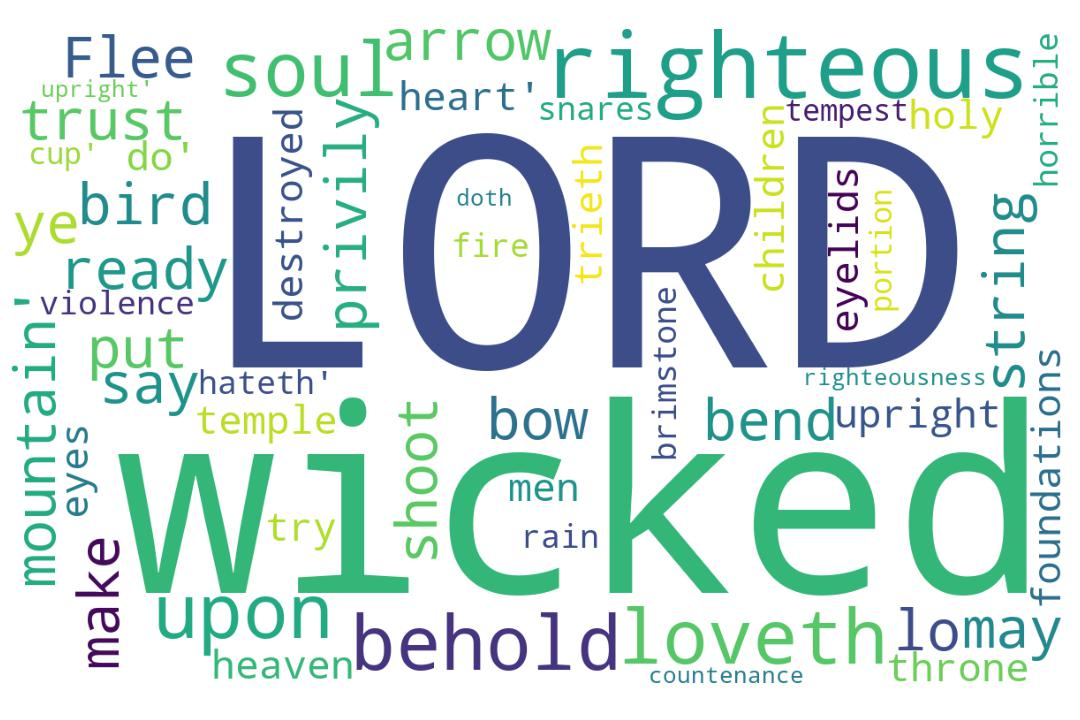
\includegraphics[width=\linewidth]{19OT-Psalms/Psalm11-WordCloud.jpg}
  \caption{Psalm 11 Word Cloud}
  \label{fig:Psalm 11 word Cloud}
\end{figure}

\marginpar{\scriptsize \centering \fcolorbox{bone}{lime}{\textbf{GOD IS WATCHING}}\\ (Psalm 11:1-7)     \begin{compactenum}[I.]
    \item He is \textbf{Interested in Paths of Mankind} \index[scripture]{Psalms!Psa 011:01}(Psa 11:1)
    \item He \textbf{Investigates the Manner of People} \index[scripture]{Psalms!Psa 011:01}(Psa 11:1)
    \item He \textbf{Intervenes is the Plans of Man} \index[scripture]{Psalms!Psa 011:02}(Psa 11:2)
    \item He \textbf{Interferes in the Programs of Evil} \index[scripture]{Psalms!Psa 011:02}(Psa 11:2)
    \item He is \textbf{Involved in the Progression of History} \index[scripture]{Psalms!Psa 011:04}(Psa 11:4)
    \item He \textbf{Invests in His Priorities}  \index[scripture]{Psalms!Psa 001:04}(Psa 11:4)
    \item He \textbf{Inhabits His Property} \index[scripture]{Psalms!Psa 011:06}(Psa 11:6)
\end{compactenum}}

\marginpar{\scriptsize \centering \fcolorbox{bone}{yellow}{\textbf{A TRIP TO SELAH PETRA}}\\ (Psalm 11:1-7)     
\begin{compactenum}[I.]
    \item The \textbf{Flight} \index[scripture]{Psalms!Psa 011:01}(Psa 11:1)
    \item The \textbf{Foe} \index[scripture]{Psalms!Psa 011:02}(Psa 11:2)
    \item The \textbf{Foundations} \index[scripture]{Psalms!Psa 011:03}(Psa 11:3)
    \item The \textbf{Fitness} Test \index[scripture]{Psalms!Psa 011:05}(Psa 11:5)
    \item The \textbf{Furor} Test \index[scripture]{Psalms!Psa 011:05}(Psa 11:5)
    \item The \textbf{Fire} \index[scripture]{Psalms!Psa 011:06}(Psa 11:6)
    \item The \textbf{Faithfulness} (of the Lord) \index[scripture]{Psalms!Psa 011:07}(Psa 11:7)
\end{compactenum}}



\footnote{\textcolor[cmyk]{0.99998,1,0,0}{\hyperlink{TOC}{Return to end of Table of Contents.}}}\footnote{\href{https://audiobible.com/bible}{\textcolor[cmyk]{0.99998,1,0,0}{Psalms Audio}}}\textcolor[cmyk]{0.99998,1,0,0}{To the chief Musician, \emph{A Psalm} of David.}\\
\\
\textcolor[cmyk]{0.99998,1,0,0}{In the LORD put I my trust: how say ye to my soul, \fcolorbox{bone}{lime}{Flee} \emph{as} a bird to your mountain?}\footnote{\textbf{Matthew 24:15-22} - \textcolor{red}{When ye therefore shall see the abomination of desolation, spoken of by Daniel the prophet, stand in the holy place, (whoso readeth, let him understand:)} [16] \textcolor{red}{Then let them which be in Judaea flee into the mountains:} [17] \textcolor{red}{Let him which is on the housetop not come down to take any thing out of his house:} [18] \textcolor{red}{Neither let him which is in the field return back to take his clothes.} [19] \textcolor{red}{And woe unto them that are with child, and to them that give suck in those days!} [20] \textcolor{red}{But pray ye that your flight be not in the winter, neither on the sabbath day:} [21] \textcolor{red}{For then shall be great tribulation, such as was not since the beginning of the world to this time, no, nor ever shall be.} [22] \textcolor{red}{And except those days should be shortened, there should no flesh be saved: but for the elect’s sake those days shall be shortened.}}\footnote{\textbf{Mark 13:14-20} - \textcolor{red}{But when ye shall see the abomination of desolation, spoken of by Daniel the prophet, standing where it ought not, (let him that readeth understand,) then let them that be in Judæa flee to the mountains:} [15] \textcolor{red}{And let him that is on the housetop not go down into the house, neither enter therein, to take any thing out of his house:} [16] \textcolor{red}{And let him that is in the field not turn back again for to take up his garment.} [17] \textcolor{red}{But woe to them that are with child, and to them that give suck in those days!} [18] \textcolor{red}{And pray ye that your flight be not in the winter.} [19] \textcolor{red}{For in those days shall be affliction, such as was not from the beginning of the creation which God created unto this time, neither shall be.} [20] \textcolor{red}{And except that the Lord had shortened those days, no flesh should be saved: but for the elect’s sake, whom he hath chosen, he hath shortened the days.}}
[2] \textcolor[cmyk]{0.99998,1,0,0}{For, lo, the wicked bend \emph{their} bow, they make ready their arrow upon the string, that they may privily shoot at the upright in heart.}
[3] \textcolor[cmyk]{0.99998,1,0,0}{If the foundations be destroyed, what can the righteous do?}
[4] \textcolor[cmyk]{0.99998,1,0,0}{The LORD \emph{is} \fcolorbox{bone}{lime}{in his holy temple}, the LORD'S throne \emph{is} in heaven: his eyes behold, \fcolorbox{bone}{lime}{his eyelids try}, the children of men.}
[5] \textcolor[cmyk]{0.99998,1,0,0}{The LORD trieth the righteous: but the wicked and him that loveth violence his soul hateth.}
[6] \textcolor[cmyk]{0.99998,1,0,0}{Upon the wicked he shall rain snares, fire and brimstone, and an horrible tempest: \emph{this} \emph{shall} \emph{be} the portion of their cup.}
[7] \textcolor[cmyk]{0.99998,1,0,0}{For the righteous LORD loveth righteousness; his countenance doth behold the upright.}


\section{Psalm 11 Comments}

\subsection{Numeric Nuggets}
\textbf{13:} The 13-letter word ``righteousness'' is found in the chapter.   
There are 13 words in Psalm 11:1b (after the colon). Those who exercise rebellion and do not flee will be destroyed.

\subsection{Psalm 11:1}
Why, if one is trusting in the Lord, does he need to flee the mountain? Because in Matthew 24:15, the Abomination of Desolation has just occurred, and Jews are told to flee. This event will kick off the second half of the Tribulation, when Antichrist unleashes terror on God's people. See also Psalm 55:6. This ``flight'' is pictured by the Exodus, when God carried Israel ``on eagles' wings'' (Exodus 19:4). \cite{Ruckman1992PsalmsV1}\footnote{\textbf{Exodus 19:4} - Ye have seen what I did unto the Egyptians, and how I bare you on eagles' wings, and brought you unto myself.}\footnote{\textbf{Psalm 55:6} - And I said, Oh that I had wings like a dove! for then would I fly away, and be at rest.}\footnote{\textbf{Matthew 24:15-16} - When ye therefore shall see the abomination of desolation, spoken of by Daniel the prophet, stand in the holy place, (whoso readeth, let him understand:) [16] Then let them which be in Judaea flee into the mountains:}


\subsection{Psalm 11:2}
These wicked are the same wicked as in Psalm 9 and 10.

\subsection{Psalm 11:3}

%\index[NWIV]{20!Psalms!Psa 11:1}\index[AWIP]{In!Psalms!Psa 11:1}\index[AWIP]{the!Psalms!Psa 11:1}\index[AWIP]{LORD!Psalms!Psa 11:1}\index[AWIP]{put!Psalms!Psa 11:1}\index[AWIP]{I!Psalms!Psa 11:1}\index[AWIP]{my!Psalms!Psa 11:1}\index[AWIP]{my!Psalms!Psa 11:1 (2)}\index[AWIP]{trust!Psalms!Psa 11:1}\index[AWIP]{how!Psalms!Psa 11:1}\index[AWIP]{say!Psalms!Psa 11:1}\index[AWIP]{ye!Psalms!Psa 11:1}\index[AWIP]{to!Psalms!Psa 11:1}\index[AWIP]{to!Psalms!Psa 11:1 (2)}\index[AWIP]{soul!Psalms!Psa 11:1}\index[AWIP]{Flee!Psalms!Psa 11:1}\index[AWIP]{\emph{as}!Psalms!Psa 11:1}\index[AWIP]{a!Psalms!Psa 11:1}\index[AWIP]{bird!Psalms!Psa 11:1}\index[AWIP]{your!Psalms!Psa 11:1}\index[AWIP]{mountain?!Psalms!Psa 11:1}\index[AWIP]{\emph{as}!Psalms!Psa 11:1}

\index[NWIV]{25!Psalms!Psa 11:2}\index[AWIP]{For!Psalms!Psa 11:2}\index[AWIP]{lo!Psalms!Psa 11:2}\index[AWIP]{the!Psalms!Psa 11:2}\index[AWIP]{the!Psalms!Psa 11:2 (2)}\index[AWIP]{the!Psalms!Psa 11:2 (3)}\index[AWIP]{wicked!Psalms!Psa 11:2}\index[AWIP]{bend!Psalms!Psa 11:2}\index[AWIP]{\emph{their}!Psalms!Psa 11:2}\index[AWIP]{bow!Psalms!Psa 11:2}\index[AWIP]{they!Psalms!Psa 11:2}\index[AWIP]{they!Psalms!Psa 11:2 (2)}\index[AWIP]{make!Psalms!Psa 11:2}\index[AWIP]{ready!Psalms!Psa 11:2}\index[AWIP]{their!Psalms!Psa 11:2}\index[AWIP]{arrow!Psalms!Psa 11:2}\index[AWIP]{upon!Psalms!Psa 11:2}\index[AWIP]{string!Psalms!Psa 11:2}\index[AWIP]{that!Psalms!Psa 11:2}\index[AWIP]{may!Psalms!Psa 11:2}\index[AWIP]{privily!Psalms!Psa 11:2}\index[AWIP]{shoot!Psalms!Psa 11:2}\index[AWIP]{at!Psalms!Psa 11:2}\index[AWIP]{upright!Psalms!Psa 11:2}\index[AWIP]{in!Psalms!Psa 11:2}\index[AWIP]{heart!Psalms!Psa 11:2}\index[AWIP]{\emph{their}!Psalms!Psa 11:2}

\index[NWIV]{10!Psalms!Psa 11:3}\index[AWIP]{If!Psalms!Psa 11:3}\index[AWIP]{the!Psalms!Psa 11:3}\index[AWIP]{the!Psalms!Psa 11:3 (2)}\index[AWIP]{foundations!Psalms!Psa 11:3}\index[AWIP]{be!Psalms!Psa 11:3}\index[AWIP]{destroyed!Psalms!Psa 11:3}\index[AWIP]{what!Psalms!Psa 11:3}\index[AWIP]{can!Psalms!Psa 11:3}\index[AWIP]{righteous!Psalms!Psa 11:3}\index[AWIP]{do?!Psalms!Psa 11:3}

\index[NWIV]{23!Psalms!Psa 11:4}\index[AWIP]{The!Psalms!Psa 11:4}\index[AWIP]{LORD!Psalms!Psa 11:4}\index[AWIP]{\emph{is}!Psalms!Psa 11:4}\index[AWIP]{\emph{is}!Psalms!Psa 11:4 (2)}\index[AWIP]{in!Psalms!Psa 11:4}\index[AWIP]{in!Psalms!Psa 11:4 (2)}\index[AWIP]{his!Psalms!Psa 11:4}\index[AWIP]{his!Psalms!Psa 11:4 (2)}\index[AWIP]{his!Psalms!Psa 11:4 (3)}\index[AWIP]{holy!Psalms!Psa 11:4}\index[AWIP]{temple!Psalms!Psa 11:4}\index[AWIP]{the!Psalms!Psa 11:4}\index[AWIP]{the!Psalms!Psa 11:4 (2)}\index[AWIP]{LORD'S!Psalms!Psa 11:4}\index[AWIP]{throne!Psalms!Psa 11:4}\index[AWIP]{heaven!Psalms!Psa 11:4}\index[AWIP]{eyes!Psalms!Psa 11:4}\index[AWIP]{behold!Psalms!Psa 11:4}\index[AWIP]{eyelids!Psalms!Psa 11:4}\index[AWIP]{try!Psalms!Psa 11:4}\index[AWIP]{children!Psalms!Psa 11:4}\index[AWIP]{of!Psalms!Psa 11:4}\index[AWIP]{men!Psalms!Psa 11:4}\index[AWIP]{\emph{is}!Psalms!Psa 11:4}\index[AWIP]{\emph{is}!Psalms!Psa 11:4 (2)}

\index[NWIV]{16!Psalms!Psa 11:5}\index[AWIP]{The!Psalms!Psa 11:5}\index[AWIP]{LORD!Psalms!Psa 11:5}\index[AWIP]{trieth!Psalms!Psa 11:5}\index[AWIP]{the!Psalms!Psa 11:5}\index[AWIP]{the!Psalms!Psa 11:5 (2)}\index[AWIP]{righteous!Psalms!Psa 11:5}\index[AWIP]{but!Psalms!Psa 11:5}\index[AWIP]{wicked!Psalms!Psa 11:5}\index[AWIP]{and!Psalms!Psa 11:5}\index[AWIP]{him!Psalms!Psa 11:5}\index[AWIP]{that!Psalms!Psa 11:5}\index[AWIP]{loveth!Psalms!Psa 11:5}\index[AWIP]{violence!Psalms!Psa 11:5}\index[AWIP]{his!Psalms!Psa 11:5}\index[AWIP]{soul!Psalms!Psa 11:5}\index[AWIP]{hateth!Psalms!Psa 11:5}

\index[NWIV]{22!Psalms!Psa 11:6}\index[AWIP]{Upon!Psalms!Psa 11:6}\index[AWIP]{the!Psalms!Psa 11:6}\index[AWIP]{the!Psalms!Psa 11:6 (2)}\index[AWIP]{wicked!Psalms!Psa 11:6}\index[AWIP]{he!Psalms!Psa 11:6}\index[AWIP]{shall!Psalms!Psa 11:6}\index[AWIP]{rain!Psalms!Psa 11:6}\index[AWIP]{snares!Psalms!Psa 11:6}\index[AWIP]{fire!Psalms!Psa 11:6}\index[AWIP]{and!Psalms!Psa 11:6}\index[AWIP]{and!Psalms!Psa 11:6 (2)}\index[AWIP]{brimstone!Psalms!Psa 11:6}\index[AWIP]{an!Psalms!Psa 11:6}\index[AWIP]{horrible!Psalms!Psa 11:6}\index[AWIP]{tempest!Psalms!Psa 11:6}\index[AWIP]{\emph{this}!Psalms!Psa 11:6}\index[AWIP]{\emph{shall}!Psalms!Psa 11:6}\index[AWIP]{\emph{be}!Psalms!Psa 11:6}\index[AWIP]{portion!Psalms!Psa 11:6}\index[AWIP]{of!Psalms!Psa 11:6}\index[AWIP]{their!Psalms!Psa 11:6}\index[AWIP]{cup!Psalms!Psa 11:6}\index[AWIP]{\emph{this}!Psalms!Psa 11:6}\index[AWIP]{\emph{shall}!Psalms!Psa 11:6}\index[AWIP]{\emph{be}!Psalms!Psa 11:6}

\index[NWIV]{12!Psalms!Psa 11:7}\index[AWIP]{For!Psalms!Psa 11:7}\index[AWIP]{the!Psalms!Psa 11:7}\index[AWIP]{the!Psalms!Psa 11:7 (2)}\index[AWIP]{righteous!Psalms!Psa 11:7}\index[AWIP]{LORD!Psalms!Psa 11:7}\index[AWIP]{loveth!Psalms!Psa 11:7}\index[AWIP]{righteousness!Psalms!Psa 11:7}\index[AWIP]{his!Psalms!Psa 11:7}\index[AWIP]{countenance!Psalms!Psa 11:7}\index[AWIP]{doth!Psalms!Psa 11:7}\index[AWIP]{behold!Psalms!Psa 11:7}\index[AWIP]{upright!Psalms!Psa 11:7}


\section{Psalm 11 Outlines}

\subsection{My Outlines}

\subsubsection{God is Watching}
\textbf{Introduction: }Remember the popular song a number of years back, ``God is Watching Us, from a Distance?'' This song has some bad theology, diestic theology, that God is sitting back, detached from mankind. The song echoes the mantra of universal-ism, where everyone is one of God's children, when only the redeemed are so. Psalm 11 tells a different story. God is at a distance, but that distance is the distance from our heads to our hearts, it is the distance of our fingers to the pages of a Bible.  God is (1) actually very near, (2) available for all who seek him, (3) apparent for those who do not choose to ignore Him:%\footnote{11 November 2014 -- \textcolor[rgb]{0.00,0.25,0.00}{\hyperlink{PsalmsTOC}{Return to end of Table of Contents.}}} 
\index[speaker]{Keith Anthony!Psalm 011 (God is Watching)}
\index[series]{Psalms (Keith Anthony)!Psalm 011 (God is Watching)}
\index[date]{2021/01/11!Psalm 011 (God is Watching) (Keith Anthony)}
\begin{compactenum}[I.]
    \item He is \textbf{Interested in Paths of Mankind} \index[scripture]{Psalms!Psa 011:01}(Psa 11:1)
    \item He \textbf{Investigates the Manner of People} \index[scripture]{Psalms!Psa 011:01}(Psa 11:1)
    \item He \textbf{Intervenes is the Plans of Man} \index[scripture]{Psalms!Psa 011:02}(Psa 11:2)
    \item He \textbf{Interferes in the Programs of Evil} \index[scripture]{Psalms!Psa 011:02}(Psa 11:2)
    \item He is \textbf{Involved in the Progression of History} \index[scripture]{Psalms!Psa 011:04}(Psa 11:4)
    \item He \textbf{Invests in His Priorities}  \index[scripture]{Psalms!Psa 001:04}(Psa 11:4)
    \item He \textbf{Inhabits His Property} \index[scripture]{Psalms!Psa 011:06}(Psa 11:6)
\end{compactenum}

\subsubsection{A Trip to Selah Petra}

\index[speaker]{Keith Anthony!Psalm 011 (A Trip to Selah Petra)}
\index[series]{Psalms (Keith Anthony)!Psalm 011 (A Trip to Selah Petra)}
\index[date]{2021/01/11!Psalm 011 (A Trip to Selah Petra) (Keith Anthony)}

\begin{compactenum}[I.]
    \item The \textbf{Flight} \index[scripture]{Psalms!Psa 011:01}(Psa 11:1)
    \item The \textbf{Foe} \index[scripture]{Psalms!Psa 011:02}(Psa 11:2)
    \item The \textbf{Foundations} \index[scripture]{Psalms!Psa 011:03}(Psa 11:3)
    \item The \textbf{Fitness} Test \index[scripture]{Psalms!Psa 011:05}(Psa 11:5)
    \item The \textbf{Furor} Test \index[scripture]{Psalms!Psa 011:05}(Psa 11:5)
    \item The \textbf{Fire} \index[scripture]{Psalms!Psa 011:06}(Psa 11:6)
    \item The \textbf{Faithfulness} (of the Lord) \index[scripture]{Psalms!Psa 011:07}(Psa 11:7)
\end{compactenum}


\subsection{Outlines from Others}

\subsubsection{The Early Life of David, in 3 Parts}
Psalm 11 can be seen the depict three phases of the early life of David.%\footnote{1 December 2014, of unknown origin}
\index[speaker]{unknown!Psalm 011 (The Early Life of David, in 3 Parts)}
\index[series]{Psalms (unknown)!Psalm 011 (The Early Life of David, in 3 Parts)}
\begin{compactenum}[I.]
    \item \textbf{The Country, The Formative Years, Learned to Worship} 
    \item \textbf{The Court, The Fateful Years, Learned Wisdom} 
    \item \textbf{The Cave, The Fugitive Years, Learned Warfare} 
\end{compactenum}


%\section{Psalm 11 Statistics}

%%%%%%%%%%%%%%%%%%%%%%%%%%%
%%%%%Word Statistics
%%%%%%%%%%%%%%%%%%%%%%%%%%%


\normalsize



\subsection{Chapter Word Statistics}


%%%%%%%%%%
%%%%%%%%%%
 
\begin{center}
\begin{longtable}{l|c|c|c|c}
\caption[Stats for Psalm 11]{Stats for Psalm 11} \label{table:Stats for Psalm 11} \\ 
\hline \multicolumn{1}{|c|}{\textbf{Verse(s)}} & \multicolumn{1}{|c|}{\textbf{Count}} & \multicolumn{1}{|c|}{\textbf{Unique}} & \multicolumn{1}{|c|}{\textbf{Italics}} & \multicolumn{1}{|c|}{\textbf{Uniq Italic}}  \\ \hline 
\endfirsthead
 
\multicolumn{5}{c}
{{\bfseries \tablename\ \thetable{} -- continued from previous page}} \\  
\hline \multicolumn{1}{|c|}{\textbf{Verse(s)}} & \multicolumn{1}{|c|}{\textbf{Count}} & \multicolumn{1}{|c|}{\textbf{Unique}} & \multicolumn{1}{|c|}{\textbf{Italics}} & \multicolumn{1}{|c|}{\textbf{Uniq Italic}}  \\ \hline 
\endhead
 
\hline \multicolumn{5}{|r|}{{Continued if needed}} \\ \hline
\endfoot 
1 & 20 & 18 & 1 & 1\\ \hline
2 & 25 & 22 & 1 & 1\\ \hline
3 & 10 & 9 & 0 & 0\\ \hline
4 & 23 & 18 & 2 & 1\\ \hline
5 & 16 & 15 & 0 & 0\\ \hline
6 & 22 & 20 & 3 & 3\\ \hline
7 & 12 & 11 & 0 & 0\\ \hline
\hline \hline
Total & 128 & 87 & 7 & 6



\end{longtable}
\end{center}

%%%%%%%%%%
%%%%%%%%%%
 
\subsection{Words by Frequency}

\begin{center}
\begin{longtable}{l|r}
\caption[Word Frequencies in Psalm 11]{Word Frequencies in Psalm 11} \label{table:WordsIn-Psalm-11} \\ 
\hline \multicolumn{1}{|c|}{\textbf{Word}} & \multicolumn{1}{c|}{\textbf{Frequency}} \\ \hline 
\endfirsthead
 
\multicolumn{2}{c}
{{\bfseries \tablename\ \thetable{} -- continued from previous page}} \\ 
\hline \multicolumn{1}{|c|}{\textbf{Word}} & \multicolumn{1}{c|}{\textbf{Frequency}} \\ \hline 
\endhead
 
\hline \multicolumn{2}{|r|}{{Continued if needed}} \\ \hline
\endfoot
 
\hline \hline
\endlastfoot
the & 14 \\ \hline
his & 5 \\ \hline
LORD & 4 \\ \hline
wicked & 3 \\ \hline
in & 3 \\ \hline
righteous & 3 \\ \hline
and & 3 \\ \hline
my & 2 \\ \hline
to & 2 \\ \hline
soul & 2 \\ \hline
For & 2 \\ \hline
they & 2 \\ \hline
their & 2 \\ \hline
that & 2 \\ \hline
upright & 2 \\ \hline
The & 2 \\ \hline
\emph{is} & 2 \\ \hline
behold & 2 \\ \hline
of & 2 \\ \hline
loveth & 2 \\ \hline
In & 1 \\ \hline
put & 1 \\ \hline
I & 1 \\ \hline
trust & 1 \\ \hline
how & 1 \\ \hline
say & 1 \\ \hline
ye & 1 \\ \hline
Flee & 1 \\ \hline
\emph{as} & 1 \\ \hline
a & 1 \\ \hline
bird & 1 \\ \hline
your & 1 \\ \hline
mountain & 1 \\ \hline
lo & 1 \\ \hline
bend & 1 \\ \hline
\emph{their} & 1 \\ \hline
bow & 1 \\ \hline
make & 1 \\ \hline
ready & 1 \\ \hline
arrow & 1 \\ \hline
upon & 1 \\ \hline
string & 1 \\ \hline
may & 1 \\ \hline
privily & 1 \\ \hline
shoot & 1 \\ \hline
at & 1 \\ \hline
heart & 1 \\ \hline
If & 1 \\ \hline
foundations & 1 \\ \hline
be & 1 \\ \hline
destroyed & 1 \\ \hline
what & 1 \\ \hline
can & 1 \\ \hline
do & 1 \\ \hline
holy & 1 \\ \hline
temple & 1 \\ \hline
LORD'S & 1 \\ \hline
throne & 1 \\ \hline
heaven & 1 \\ \hline
eyes & 1 \\ \hline
eyelids & 1 \\ \hline
try & 1 \\ \hline
children & 1 \\ \hline
men & 1 \\ \hline
trieth & 1 \\ \hline
but & 1 \\ \hline
him & 1 \\ \hline
violence & 1 \\ \hline
hateth & 1 \\ \hline
Upon & 1 \\ \hline
he & 1 \\ \hline
shall & 1 \\ \hline
rain & 1 \\ \hline
snares & 1 \\ \hline
fire & 1 \\ \hline
brimstone & 1 \\ \hline
an & 1 \\ \hline
horrible & 1 \\ \hline
tempest & 1 \\ \hline
\emph{this} & 1 \\ \hline
\emph{shall} & 1 \\ \hline
\emph{be} & 1 \\ \hline
portion & 1 \\ \hline
cup & 1 \\ \hline
righteousness & 1 \\ \hline
countenance & 1 \\ \hline
doth & 1 \\ \hline
\end{longtable}
\end{center}



\normalsize



\subsection{Words Alphabetically}

\begin{center}
\begin{longtable}{l|r}
\caption[Word Alphabetically in Psalm 11]{Word Alphabetically in Psalm 11} \label{table:WordsIn-Psalm-11} \\ 
\hline \multicolumn{1}{|c|}{\textbf{Word}} & \multicolumn{1}{c|}{\textbf{Frequency}} \\ \hline 
\endfirsthead
 
\multicolumn{2}{c}
{{\bfseries \tablename\ \thetable{} -- continued from previous page}} \\ 
\hline \multicolumn{1}{|c|}{\textbf{Word}} & \multicolumn{1}{c|}{\textbf{Frequency}} \\ \hline 
\endhead
 
\hline \multicolumn{2}{|r|}{{Continued if needed}} \\ \hline
\endfoot
 
\hline \hline
\endlastfoot
Flee & 1 \\ \hline
For & 2 \\ \hline
I & 1 \\ \hline
If & 1 \\ \hline
In & 1 \\ \hline
LORD & 4 \\ \hline
LORD'S & 1 \\ \hline
The & 2 \\ \hline
Upon & 1 \\ \hline
\emph{as} & 1 \\ \hline
\emph{be} & 1 \\ \hline
\emph{is} & 2 \\ \hline
\emph{shall} & 1 \\ \hline
\emph{their} & 1 \\ \hline
\emph{this} & 1 \\ \hline
a & 1 \\ \hline
an & 1 \\ \hline
and & 3 \\ \hline
arrow & 1 \\ \hline
at & 1 \\ \hline
be & 1 \\ \hline
behold & 2 \\ \hline
bend & 1 \\ \hline
bird & 1 \\ \hline
bow & 1 \\ \hline
brimstone & 1 \\ \hline
but & 1 \\ \hline
can & 1 \\ \hline
children & 1 \\ \hline
countenance & 1 \\ \hline
cup & 1 \\ \hline
destroyed & 1 \\ \hline
do & 1 \\ \hline
doth & 1 \\ \hline
eyelids & 1 \\ \hline
eyes & 1 \\ \hline
fire & 1 \\ \hline
foundations & 1 \\ \hline
hateth & 1 \\ \hline
he & 1 \\ \hline
heart & 1 \\ \hline
heaven & 1 \\ \hline
him & 1 \\ \hline
his & 5 \\ \hline
holy & 1 \\ \hline
horrible & 1 \\ \hline
how & 1 \\ \hline
in & 3 \\ \hline
lo & 1 \\ \hline
loveth & 2 \\ \hline
make & 1 \\ \hline
may & 1 \\ \hline
men & 1 \\ \hline
mountain & 1 \\ \hline
my & 2 \\ \hline
of & 2 \\ \hline
portion & 1 \\ \hline
privily & 1 \\ \hline
put & 1 \\ \hline
rain & 1 \\ \hline
ready & 1 \\ \hline
righteous & 3 \\ \hline
righteousness & 1 \\ \hline
say & 1 \\ \hline
shall & 1 \\ \hline
shoot & 1 \\ \hline
snares & 1 \\ \hline
soul & 2 \\ \hline
string & 1 \\ \hline
tempest & 1 \\ \hline
temple & 1 \\ \hline
that & 2 \\ \hline
the & 14 \\ \hline
their & 2 \\ \hline
they & 2 \\ \hline
throne & 1 \\ \hline
to & 2 \\ \hline
trieth & 1 \\ \hline
trust & 1 \\ \hline
try & 1 \\ \hline
upon & 1 \\ \hline
upright & 2 \\ \hline
violence & 1 \\ \hline
what & 1 \\ \hline
wicked & 3 \\ \hline
ye & 1 \\ \hline
your & 1 \\ \hline
\end{longtable}
\end{center}



\normalsize



\subsection{Word Lengths in Chapter}
\normalsize
\begin{longtable}{l|p{3.75in}}
\caption[Words by Length in Psalm 11]{Words by Length in Psalm 11} \label{table:WordsIn-Psalm-11} \\ 
\hline \multicolumn{1}{|c|}{\textbf{Length}} & \multicolumn{1}{c|}{\textbf{Words}} \\ \hline 
\endfirsthead
 
\multicolumn{2}{c}
{{\bfseries \tablename\ \thetable{} -- continued from previous page}} \\ 
\hline \multicolumn{1}{|c|}{\textbf{Length}} & \multicolumn{1}{c|}{\textbf{Words}} \\ \hline 
\endhead
 
\hline \multicolumn{2}{|r|}{{Continued if needed}} \\ \hline
\endfoot
 
\hline \hline
\endlastfoot
1 & I, a \\ \hline
2 & In, my, ye, to, \emph{as}, lo, at, in, If, be, do, \emph{is}, of, he, an, \emph{be} \\ \hline
3 & the, put, how, say, For, bow, may, can, The, his, try, men, but, and, him, cup \\ \hline
4 & LORD, soul, Flee, bird, your, bend, they, make, upon, that, what, holy, eyes, Upon, rain, fire, \emph{this}, doth \\ \hline
5 & trust, \emph{their}, ready, their, arrow, shoot, heart, shall, \emph{shall} \\ \hline
6 & wicked, string, temple, LORD'S, throne, heaven, behold, trieth, loveth, hateth, snares \\ \hline
7 & privily, upright, eyelids, tempest, portion \\ \hline
8 & mountain, children, violence, horrible \\ \hline
9 & destroyed, righteous, brimstone \\ \hline
11 & foundations, countenance \\ \hline
13 & righteousness \\ \hline
\end{longtable}






%%%%%%%%%%
%%%%%%%%%%
\subsection{Psalm 11 Repeated Phrases}


%%%%%%%%%%
%%%%%%%%%%
\normalsize
 
\begin{center}
\begin{longtable}{|p{3.0in}|p{0.5in}|}
\caption[Psalm 11 Repeated Phrases]{Psalm 11 Repeated Phrases}\label{table:Repeated Phrases Psalm 11} \\
\hline \multicolumn{1}{|c|}{\textbf{Phrase}} & \multicolumn{1}{c|}{\textbf{Frequency}} \\ \hline 
\endfirsthead
 
\multicolumn{2}{c}
{{\bfseries \tablename\ \thetable{} -- continued from previous page}} \\  
\hline \multicolumn{1}{|c|}{\textbf{Phrase}} & \multicolumn{1}{c|}{\textbf{Frequency}} \\ \hline 
\endhead
 
\hline \multicolumn{2}{c}{{ }} \\ \hline
\endfoot 
the wicked & 3\\ \hline 
the righteous & 3\\ \hline 
\end{longtable}
\end{center}



%%%%%%%%%%
%%%%%%%%%%




\chapter{Psalm 12}

\begin{figure}
  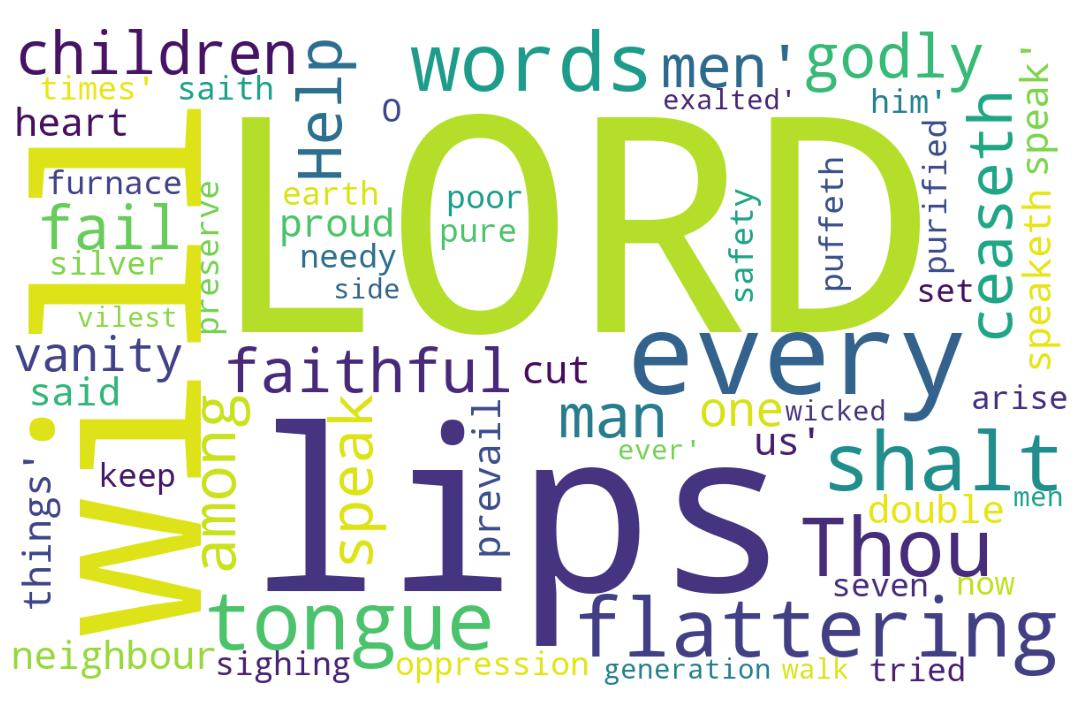
\includegraphics[width=\linewidth]{19OT-Psalms/Psalm12-WordCloud.jpg}
  \caption{Psalm 12 Word Cloud}
  \label{fig:Psalm 12 word Cloud}
\end{figure}


\marginpar{\scriptsize \centering \fcolorbox{bone}{lime}{\textbf{WORDS FROM THE LORD}}\\ (Psalm 12:1--8)     \begin{compactenum}[I.]
    \item \textbf{Provoked Words} \index[scripture]{Psalms!Psa 012:05}\index[scripture]{Psalms!Psa 012:01}(Psa 12:1, 5) (for the ...)
    \item \textbf{Proving Words} \index[scripture]{Psalms!Psa 012:05}(Psa 12:5) (now will I arise)
    \item \textbf{Protecting Words} \index[scripture]{Psalms!Psa 012:05}(Psa 12:5) (safety)
    \item \textbf{Prevailing Words} \index[scripture]{Psalms!Psa 012:05}(Psa 12:5) (Thou shall keep them)
    \item \textbf{Precious Words} \index[scripture]{Psalms!Psa 012:06}(Psa 12:6) (silver)
    \item \textbf{Preserved Words} \index[scripture]{Psalms!Psa 012:07}(Psa 12:7) (From this generation)
    \item \textbf{Permanent Words} \index[scripture]{Psalms!Psa 012:07}(Psa 12:7)
\end{compactenum}}

\textcolor[cmyk]{0.99998,1,0,0}{To the chief Musician upon Sheminith, A Psalm of David.}\\
\\
\footnote{\textcolor[cmyk]{0.99998,1,0,0}{\hyperlink{TOC}{Return to end of Table of Contents.}}}\footnote{\href{https://www.audioverse.org/english/audiobibles/books/ENGKJV/O/Ps/1}{\textcolor[cmyk]{0.99998,1,0,0}{Psalms Audio}}}\textcolor[cmyk]{0.99998,1,0,0}{Help, LORD; \fcolorbox{bone}{lime}{for the} godly man ceaseth; for the faithful fail from among the children of men.}
[2] \textcolor[cmyk]{0.99998,1,0,0}{They speak vanity every one with his neighbour: \emph{with} flattering lips \emph{and} with a double heart do they speak.}
[3] \textcolor[cmyk]{0.99998,1,0,0}{The LORD shall cut off all flattering lips, \emph{and} the tongue that speaketh proud things:}
[4] \textcolor[cmyk]{0.99998,1,0,0}{Who have said, With our tongue will we prevail; our lips \emph{are} our own: who \emph{is} lord over us?}
[5] \textcolor[cmyk]{0.99998,1,0,0}{\fcolorbox{bone}{lime}{For the} oppression of the poor, for the sighing of the needy, \fcolorbox{bone}{lime}{now will I arise}, saith the LORD; I will set \emph{him} in \fcolorbox{bone}{lime}{safety} \emph{from} \emph{him} \emph{that} puffeth at him.}\footnote{\textbf{Psalm 10:5} - His ways are always grievous; thy judgments are far above out of his sight: as for all his enemies, he puffeth at them.}\footnote{\textbf{1 Corinthians 8:1} - Now as touching things offered unto idols, we know that we all have knowledge. Knowledge puffeth up, but charity edifieth.}\footnote{\textbf{Job 3:24} - 
For my sighing cometh before I eat, and my roarings are poured out like the waters.}\footnote{\textbf{Psalm 31:10} - For my life is spent with grief, and my years with sighing: my strength faileth because of mine iniquity, and my bones are consumed.}\footnote{\textbf{Psalm 79:11} - Let the sighing of the prisoner come before thee; according to the greatness of thy power preserve thou those that are appointed to die;}\footnote{\textbf{Isaiah 35:1} - 
And the ransomed of the Lord shall return, and come to Zion with songs and everlasting joy upon their heads: they shall obtain joy and gladness, and sorrow and sighing shall flee away.}\footnote{\textbf{Jeremiah 45:3} - 
Thou didst say, Woe is me now! for the Lord hath added grief to my sorrow; I fainted in my sighing, and I find no rest.}
[6] \textcolor[cmyk]{0.99998,1,0,0}{The words of the LORD \emph{are} pure words: \emph{as} \fcolorbox{bone}{lime}{silver} tried in a furnace of earth, purified seven times.}
[7] \textcolor[cmyk]{0.99998,1,0,0}{Thou shalt keep them, O LORD, thou shalt \fcolorbox{bone}{lime}{preserve} them \fcolorbox{bone}{lime}{from this generation} for ever.}
[8] \textcolor[cmyk]{0.99998,1,0,0}{The wicked walk on every side, when the vilest men are exalted.}
\section{Psalm 12 Comments}

\subsection{Numeric Nuggets}
\textbf{13:} Verse 13 has 13 unique words.


\subsection{Psalm 12:7}
Modern version corrupt the verse as seen in Table~\ref{table:Corruption Psalm 12:7}

\begin{center}

\begin{table}[ht]
\centering
\begin{tabular}{|p{.5in}|p{3.5in}|}
    \hline
\textcolor[rgb]{0.00,0.00,1.00}{AV} & \textcolor[rgb]{0.00,0.00,1.00}{Thou shalt keep them, O LORD, thou shalt preserve them from this generation for ever.} \\ \hline
%%
ASV &  Thou wilt keep them, O Jehovah, Thou wilt preserve them from this generation for ever.\\ \hline
%
CEB &  You, Lord, will keep us, protecting us from this generation forever.\\ \hline
%&
ESV & You, O Lord, will keep them;  you will guard us from this generation forever.\\ \hline
%
NASV &  You, O Lord, will keep them; You will preserve him from this generation forever.\\ \hline
%
MEV & You will keep them, O Lord;  You will preserve them from this generation.\\ \hline
%
NIV &  You, Lord, will keep the needy safe  and will protect us forever from the wicked, \\ \hline
%
NKJV &  You shall keep them, O Lord, You shall preserve them from this generation forever.\\ \hline
%
RSV &  Do thou, O Lord, protect us,  guard us ever from this generation.\\ \hline
 \hline

\multicolumn{2}{|p{4.3in}|}{{\textcolor{jungle}{Some translation remove the pronoun ``them'', referring back to the ``words of the Lord'' in verse 6. This attacks the doctrine of scriptural preservation. Verses 6-7 reveal the attack on the word of God, something Paul warned about in 2 Corinthians 2:17.\cite{Ruckman1992PsalmsV1}.}}} \\ \hline

\end{tabular}
\caption[Corruption Alert: Psalm 12:7]{Corruption Alert: Psalm 12:7} \label{table:Corruption Psalm 12:7}

\end{table}

\end{center}


%\index[NWIV]{17!Psalms!Psa 12:1}\index[AWIP]{Help!Psalms!Psa 12:1}\index[AWIP]{LORD!Psalms!Psa 12:1}\index[AWIP]{for!Psalms!Psa 12:1}\index[AWIP]{for!Psalms!Psa 12:1 (2)}\index[AWIP]{the!Psalms!Psa 12:1}\index[AWIP]{the!Psalms!Psa 12:1 (2)}\index[AWIP]{the!Psalms!Psa 12:1 (3)}\index[AWIP]{godly!Psalms!Psa 12:1}\index[AWIP]{man!Psalms!Psa 12:1}\index[AWIP]{ceaseth!Psalms!Psa 12:1}\index[AWIP]{faithful!Psalms!Psa 12:1}\index[AWIP]{fail!Psalms!Psa 12:1}\index[AWIP]{from!Psalms!Psa 12:1}\index[AWIP]{among!Psalms!Psa 12:1}\index[AWIP]{children!Psalms!Psa 12:1}\index[AWIP]{of!Psalms!Psa 12:1}\index[AWIP]{men!Psalms!Psa 12:1}

\index[NWIV]{19!Psalms!Psa 12:2}\index[AWIP]{They!Psalms!Psa 12:2}\index[AWIP]{speak!Psalms!Psa 12:2}\index[AWIP]{speak!Psalms!Psa 12:2 (2)}\index[AWIP]{vanity!Psalms!Psa 12:2}\index[AWIP]{every!Psalms!Psa 12:2}\index[AWIP]{one!Psalms!Psa 12:2}\index[AWIP]{with!Psalms!Psa 12:2}\index[AWIP]{with!Psalms!Psa 12:2 (2)}\index[AWIP]{his!Psalms!Psa 12:2}\index[AWIP]{neighbour!Psalms!Psa 12:2}\index[AWIP]{\emph{with}!Psalms!Psa 12:2}\index[AWIP]{flattering!Psalms!Psa 12:2}\index[AWIP]{lips!Psalms!Psa 12:2}\index[AWIP]{\emph{and}!Psalms!Psa 12:2}\index[AWIP]{a!Psalms!Psa 12:2}\index[AWIP]{double!Psalms!Psa 12:2}\index[AWIP]{heart!Psalms!Psa 12:2}\index[AWIP]{do!Psalms!Psa 12:2}\index[AWIP]{they!Psalms!Psa 12:2}\index[AWIP]{\emph{with}!Psalms!Psa 12:2}\index[AWIP]{\emph{and}!Psalms!Psa 12:2}

\index[NWIV]{15!Psalms!Psa 12:3}\index[AWIP]{The!Psalms!Psa 12:3}\index[AWIP]{LORD!Psalms!Psa 12:3}\index[AWIP]{shall!Psalms!Psa 12:3}\index[AWIP]{cut!Psalms!Psa 12:3}\index[AWIP]{off!Psalms!Psa 12:3}\index[AWIP]{all!Psalms!Psa 12:3}\index[AWIP]{flattering!Psalms!Psa 12:3}\index[AWIP]{lips!Psalms!Psa 12:3}\index[AWIP]{\emph{and}!Psalms!Psa 12:3}\index[AWIP]{the!Psalms!Psa 12:3}\index[AWIP]{tongue!Psalms!Psa 12:3}\index[AWIP]{that!Psalms!Psa 12:3}\index[AWIP]{speaketh!Psalms!Psa 12:3}\index[AWIP]{proud!Psalms!Psa 12:3}\index[AWIP]{things!Psalms!Psa 12:3}\index[AWIP]{\emph{and}!Psalms!Psa 12:3}

\index[NWIV]{19!Psalms!Psa 12:4}\index[AWIP]{Who!Psalms!Psa 12:4}\index[AWIP]{have!Psalms!Psa 12:4}\index[AWIP]{said!Psalms!Psa 12:4}\index[AWIP]{With!Psalms!Psa 12:4}\index[AWIP]{our!Psalms!Psa 12:4}\index[AWIP]{our!Psalms!Psa 12:4 (2)}\index[AWIP]{our!Psalms!Psa 12:4 (3)}\index[AWIP]{tongue!Psalms!Psa 12:4}\index[AWIP]{will!Psalms!Psa 12:4}\index[AWIP]{we!Psalms!Psa 12:4}\index[AWIP]{prevail!Psalms!Psa 12:4}\index[AWIP]{lips!Psalms!Psa 12:4}\index[AWIP]{\emph{are}!Psalms!Psa 12:4}\index[AWIP]{own!Psalms!Psa 12:4}\index[AWIP]{who!Psalms!Psa 12:4}\index[AWIP]{\emph{is}!Psalms!Psa 12:4}\index[AWIP]{lord!Psalms!Psa 12:4}\index[AWIP]{over!Psalms!Psa 12:4}\index[AWIP]{us?!Psalms!Psa 12:4}\index[AWIP]{\emph{are}!Psalms!Psa 12:4}\index[AWIP]{\emph{is}!Psalms!Psa 12:4}

\index[NWIV]{31!Psalms!Psa 12:5}\index[AWIP]{For!Psalms!Psa 12:5}\index[AWIP]{the!Psalms!Psa 12:5}\index[AWIP]{the!Psalms!Psa 12:5 (2)}\index[AWIP]{the!Psalms!Psa 12:5 (3)}\index[AWIP]{the!Psalms!Psa 12:5 (4)}\index[AWIP]{the!Psalms!Psa 12:5 (5)}\index[AWIP]{oppression!Psalms!Psa 12:5}\index[AWIP]{of!Psalms!Psa 12:5}\index[AWIP]{of!Psalms!Psa 12:5 (2)}\index[AWIP]{poor!Psalms!Psa 12:5}\index[AWIP]{for!Psalms!Psa 12:5}\index[AWIP]{sighing!Psalms!Psa 12:5}\index[AWIP]{needy!Psalms!Psa 12:5}\index[AWIP]{now!Psalms!Psa 12:5}\index[AWIP]{will!Psalms!Psa 12:5}\index[AWIP]{will!Psalms!Psa 12:5 (2)}\index[AWIP]{I!Psalms!Psa 12:5}\index[AWIP]{I!Psalms!Psa 12:5 (2)}\index[AWIP]{arise!Psalms!Psa 12:5}\index[AWIP]{saith!Psalms!Psa 12:5}\index[AWIP]{LORD!Psalms!Psa 12:5}\index[AWIP]{set!Psalms!Psa 12:5}\index[AWIP]{\emph{him}!Psalms!Psa 12:5}\index[AWIP]{\emph{him}!Psalms!Psa 12:5 (2)}\index[AWIP]{in!Psalms!Psa 12:5}\index[AWIP]{safety!Psalms!Psa 12:5}\index[AWIP]{\emph{from}!Psalms!Psa 12:5}\index[AWIP]{\emph{that}!Psalms!Psa 12:5}\index[AWIP]{puffeth!Psalms!Psa 12:5}\index[AWIP]{at!Psalms!Psa 12:5}\index[AWIP]{him!Psalms!Psa 12:5}\index[AWIP]{\emph{him}!Psalms!Psa 12:5}\index[AWIP]{\emph{him}!Psalms!Psa 12:5 (2)}\index[AWIP]{\emph{from}!Psalms!Psa 12:5}\index[AWIP]{\emph{that}!Psalms!Psa 12:5}

\index[NWIV]{19!Psalms!Psa 12:6}\index[AWIP]{The!Psalms!Psa 12:6}\index[AWIP]{words!Psalms!Psa 12:6}\index[AWIP]{words!Psalms!Psa 12:6 (2)}\index[AWIP]{of!Psalms!Psa 12:6}\index[AWIP]{of!Psalms!Psa 12:6 (2)}\index[AWIP]{the!Psalms!Psa 12:6}\index[AWIP]{LORD!Psalms!Psa 12:6}\index[AWIP]{\emph{are}!Psalms!Psa 12:6}\index[AWIP]{pure!Psalms!Psa 12:6}\index[AWIP]{\emph{as}!Psalms!Psa 12:6}\index[AWIP]{silver!Psalms!Psa 12:6}\index[AWIP]{tried!Psalms!Psa 12:6}\index[AWIP]{in!Psalms!Psa 12:6}\index[AWIP]{a!Psalms!Psa 12:6}\index[AWIP]{furnace!Psalms!Psa 12:6}\index[AWIP]{earth!Psalms!Psa 12:6}\index[AWIP]{purified!Psalms!Psa 12:6}\index[AWIP]{seven!Psalms!Psa 12:6}\index[AWIP]{times!Psalms!Psa 12:6}\index[AWIP]{\emph{are}!Psalms!Psa 12:6}\index[AWIP]{\emph{as}!Psalms!Psa 12:6}

\index[NWIV]{15!Psalms!Psa 12:7}\index[AWIP]{Thou!Psalms!Psa 12:7}\index[AWIP]{shalt!Psalms!Psa 12:7}\index[AWIP]{shalt!Psalms!Psa 12:7 (2)}\index[AWIP]{keep!Psalms!Psa 12:7}\index[AWIP]{them!Psalms!Psa 12:7}\index[AWIP]{them!Psalms!Psa 12:7 (2)}\index[AWIP]{O!Psalms!Psa 12:7}\index[AWIP]{LORD!Psalms!Psa 12:7}\index[AWIP]{thou!Psalms!Psa 12:7}\index[AWIP]{preserve!Psalms!Psa 12:7}\index[AWIP]{from!Psalms!Psa 12:7}\index[AWIP]{this!Psalms!Psa 12:7}\index[AWIP]{generation!Psalms!Psa 12:7}\index[AWIP]{for!Psalms!Psa 12:7}\index[AWIP]{ever!Psalms!Psa 12:7}

\index[NWIV]{12!Psalms!Psa 12:8}\index[AWIP]{The!Psalms!Psa 12:8}\index[AWIP]{wicked!Psalms!Psa 12:8}\index[AWIP]{walk!Psalms!Psa 12:8}\index[AWIP]{on!Psalms!Psa 12:8}\index[AWIP]{every!Psalms!Psa 12:8}\index[AWIP]{side!Psalms!Psa 12:8}\index[AWIP]{when!Psalms!Psa 12:8}\index[AWIP]{the!Psalms!Psa 12:8}\index[AWIP]{vilest!Psalms!Psa 12:8}\index[AWIP]{men!Psalms!Psa 12:8}\index[AWIP]{are!Psalms!Psa 12:8}\index[AWIP]{exalted!Psalms!Psa 12:8}


\section{Psalm 12 Outlines}

\subsection{My Outlines}

\subsubsection{These Words from the Lord}
%Psalm 8:\footnote{unknown, Keith Anthony}
\index[speaker]{Keith Anthony!Psalm 012 (These Words from the Lord)}
\index[series]{Psalms (Keith Anthony)!Psalm 012 (These Words from the Lord)}
\index[date]{2016/11/23!Psalm 012 (These Words from the Lord) (Keith Anthony)}
\textbf{Introduction: }They are:\\
\begin{compactenum}[I.]
    \item \textbf{Provoked Words} \index[scripture]{Psalms!Psa 012:05}\index[scripture]{Psalms!Psa 012:01} (Psa 12:1, 5) (for the ...)
    \item \textbf{Proving Words} \index[scripture]{Psalms!Psa 012:05} (Psa 12:5) (now will I arise)
    \item \textbf{Protecting Words} \index[scripture]{Psalms!Psa 012:05} (Psa 12:5) (safety)
    \item \textbf{Prevailing Words} \index[scripture]{Psalms!Psa 012:05} (Psa 12:5) (Thou shall keep them)
    \item \textbf{Precious Words} \index[scripture]{Psalms!Psa 012:06} (Psa 12:6) (silver)
    \item \textbf{Preserved Words} \index[scripture]{Psalms!Psa 012:07} (Psa 12:7) (From this generation)
    \item \textbf{Permanent Words} \index[scripture]{Psalms!Psa 012:07} (Psa 12:7)
\end{compactenum}



\subsection{Outlines from Others}

\subsubsection{Perspectives of a Godly Man}
Psalm 12 gives us the perspectives of a godly man:
\begin{compactenum}[I.]
    \item We see the \textbf{Godly who seem to be Perishing in the Way} \index[scripture]{Psalms!Psa 012:01} (Psalm 12:1)
    \begin{compactenum}[A.]
    	\item David watched \textbf{Prevailing Wickedness} \index[scripture]{Psalms!Psa 012:03} (Psalm 12:3)
		\item David watched the \textbf{Proud Tongues Wagging} \index[scripture]{Psalms!Psa 012:03} (Psalm 12:3) \newline but, then, 
    \end{compactenum}	
    \item David saw a \textbf{Protected Walk} \index[scripture]{Psalms!Psa 012:05} (Psalm 12:5)
	\begin{compactenum}[A.]
    \item David saw the \textbf{Puffers walled off} \index[scripture]{Psalms!Psa 012:05} (Psalm 12:5)
    \item David saw the \textbf{Purified Words} \index[scripture]{Psalms!Psa 012:06} (Psalm 12:6)
    \item David saw the \textbf{Preserved Wisdom} \index[scripture]{Psalms!Psa 012:06} (Psalm 12:6)
    \end{compactenum}
\end{compactenum}






%\section{Psalm 12 Statistics}

%%%%%%%%%%%%%%%%%%%%%%%%%%%
%%%%%Word Statistics
%%%%%%%%%%%%%%%%%%%%%%%%%%%


\normalsize



\subsection{Chapter Word Statistics}


%%%%%%%%%%
%%%%%%%%%%
 
\begin{center}
\begin{longtable}{l|c|c|c|c}
\caption[Stats for Psalm 12]{Stats for Psalm 12} \label{table:Stats for Psalm 12} \\ 
\hline \multicolumn{1}{|c|}{\textbf{Verse(s)}} & \multicolumn{1}{|c|}{\textbf{Count}} & \multicolumn{1}{|c|}{\textbf{Unique}} & \multicolumn{1}{|c|}{\textbf{Italics}} & \multicolumn{1}{|c|}{\textbf{Uniq Italic}}  \\ \hline 
\endfirsthead
 
\multicolumn{5}{c}
{{\bfseries \tablename\ \thetable{} -- continued from previous page}} \\  
\hline \multicolumn{1}{|c|}{\textbf{Verse(s)}} & \multicolumn{1}{|c|}{\textbf{Count}} & \multicolumn{1}{|c|}{\textbf{Unique}} & \multicolumn{1}{|c|}{\textbf{Italics}} & \multicolumn{1}{|c|}{\textbf{Uniq Italic}}  \\ \hline 
\endhead
 
\hline \multicolumn{5}{|r|}{{Continued if needed}} \\ \hline
\endfoot 
1 & 17 & 14 & 0 & 0\\ \hline
2 & 19 & 17 & 2 & 2\\ \hline
3 & 15 & 15 & 1 & 1\\ \hline
4 & 19 & 17 & 2 & 2\\ \hline
5 & 31 & 23 & 4 & 3\\ \hline
6 & 19 & 17 & 2 & 2\\ \hline
7 & 15 & 13 & 0 & 0\\ \hline
8 & 12 & 12 & 0 & 0\\ \hline
\hline \hline
Total & 147 & 102 & 11 & 8



\end{longtable}
\end{center}

%%%%%%%%%%
%%%%%%%%%%
 
\subsection{Words by Frequency}

\begin{center}
\begin{longtable}{l|r}
\caption[Word Frequencies in Psalm 12]{Word Frequencies in Psalm 12} \label{table:WordsIn-Psalm-12} \\ 
\hline \multicolumn{1}{|c|}{\textbf{Word}} & \multicolumn{1}{c|}{\textbf{Frequency}} \\ \hline 
\endfirsthead
 
\multicolumn{2}{c}
{{\bfseries \tablename\ \thetable{} -- continued from previous page}} \\ 
\hline \multicolumn{1}{|c|}{\textbf{Word}} & \multicolumn{1}{c|}{\textbf{Frequency}} \\ \hline 
\endhead
 
\hline \multicolumn{2}{|r|}{{Continued if needed}} \\ \hline
\endfoot
 
\hline \hline
\endlastfoot
the & 11 \\ \hline
LORD & 5 \\ \hline
of & 5 \\ \hline
for & 4 \\ \hline
lips & 3 \\ \hline
The & 3 \\ \hline
our & 3 \\ \hline
will & 3 \\ \hline
from & 2 \\ \hline
men & 2 \\ \hline
speak & 2 \\ \hline
every & 2 \\ \hline
with & 2 \\ \hline
flattering & 2 \\ \hline
\emph{and} & 2 \\ \hline
a & 2 \\ \hline
tongue & 2 \\ \hline
\emph{are} & 2 \\ \hline
I & 2 \\ \hline
\emph{him} & 2 \\ \hline
in & 2 \\ \hline
words & 2 \\ \hline
shalt & 2 \\ \hline
them & 2 \\ \hline
Help & 1 \\ \hline
godly & 1 \\ \hline
man & 1 \\ \hline
ceaseth & 1 \\ \hline
faithful & 1 \\ \hline
fail & 1 \\ \hline
among & 1 \\ \hline
children & 1 \\ \hline
They & 1 \\ \hline
vanity & 1 \\ \hline
one & 1 \\ \hline
his & 1 \\ \hline
neighbour & 1 \\ \hline
\emph{with} & 1 \\ \hline
double & 1 \\ \hline
heart & 1 \\ \hline
do & 1 \\ \hline
they & 1 \\ \hline
shall & 1 \\ \hline
cut & 1 \\ \hline
off & 1 \\ \hline
all & 1 \\ \hline
that & 1 \\ \hline
speaketh & 1 \\ \hline
proud & 1 \\ \hline
things & 1 \\ \hline
Who & 1 \\ \hline
have & 1 \\ \hline
said & 1 \\ \hline
With & 1 \\ \hline
we & 1 \\ \hline
prevail & 1 \\ \hline
own & 1 \\ \hline
who & 1 \\ \hline
\emph{is} & 1 \\ \hline
lord & 1 \\ \hline
over & 1 \\ \hline
us & 1 \\ \hline
For & 1 \\ \hline
oppression & 1 \\ \hline
poor & 1 \\ \hline
sighing & 1 \\ \hline
needy & 1 \\ \hline
now & 1 \\ \hline
arise & 1 \\ \hline
saith & 1 \\ \hline
set & 1 \\ \hline
safety & 1 \\ \hline
\emph{from} & 1 \\ \hline
\emph{that} & 1 \\ \hline
puffeth & 1 \\ \hline
at & 1 \\ \hline
him & 1 \\ \hline
pure & 1 \\ \hline
\emph{as} & 1 \\ \hline
silver & 1 \\ \hline
tried & 1 \\ \hline
furnace & 1 \\ \hline
earth & 1 \\ \hline
purified & 1 \\ \hline
seven & 1 \\ \hline
times & 1 \\ \hline
Thou & 1 \\ \hline
keep & 1 \\ \hline
O & 1 \\ \hline
thou & 1 \\ \hline
preserve & 1 \\ \hline
this & 1 \\ \hline
generation & 1 \\ \hline
ever & 1 \\ \hline
wicked & 1 \\ \hline
walk & 1 \\ \hline
on & 1 \\ \hline
side & 1 \\ \hline
when & 1 \\ \hline
vilest & 1 \\ \hline
are & 1 \\ \hline
exalted & 1 \\ \hline
\end{longtable}
\end{center}



\normalsize



\subsection{Words Alphabetically}

\begin{center}
\begin{longtable}{l|r}
\caption[Word Alphabetically in Psalm 12]{Word Alphabetically in Psalm 12} \label{table:WordsIn-Psalm-12} \\ 
\hline \multicolumn{1}{|c|}{\textbf{Word}} & \multicolumn{1}{c|}{\textbf{Frequency}} \\ \hline 
\endfirsthead
 
\multicolumn{2}{c}
{{\bfseries \tablename\ \thetable{} -- continued from previous page}} \\ 
\hline \multicolumn{1}{|c|}{\textbf{Word}} & \multicolumn{1}{c|}{\textbf{Frequency}} \\ \hline 
\endhead
 
\hline \multicolumn{2}{|r|}{{Continued if needed}} \\ \hline
\endfoot
 
\hline \hline
\endlastfoot
For & 1 \\ \hline
Help & 1 \\ \hline
I & 2 \\ \hline
LORD & 5 \\ \hline
O & 1 \\ \hline
The & 3 \\ \hline
They & 1 \\ \hline
Thou & 1 \\ \hline
Who & 1 \\ \hline
With & 1 \\ \hline
\emph{and} & 2 \\ \hline
\emph{are} & 2 \\ \hline
\emph{as} & 1 \\ \hline
\emph{from} & 1 \\ \hline
\emph{him} & 2 \\ \hline
\emph{is} & 1 \\ \hline
\emph{that} & 1 \\ \hline
\emph{with} & 1 \\ \hline
a & 2 \\ \hline
all & 1 \\ \hline
among & 1 \\ \hline
are & 1 \\ \hline
arise & 1 \\ \hline
at & 1 \\ \hline
ceaseth & 1 \\ \hline
children & 1 \\ \hline
cut & 1 \\ \hline
do & 1 \\ \hline
double & 1 \\ \hline
earth & 1 \\ \hline
ever & 1 \\ \hline
every & 2 \\ \hline
exalted & 1 \\ \hline
fail & 1 \\ \hline
faithful & 1 \\ \hline
flattering & 2 \\ \hline
for & 4 \\ \hline
from & 2 \\ \hline
furnace & 1 \\ \hline
generation & 1 \\ \hline
godly & 1 \\ \hline
have & 1 \\ \hline
heart & 1 \\ \hline
him & 1 \\ \hline
his & 1 \\ \hline
in & 2 \\ \hline
keep & 1 \\ \hline
lips & 3 \\ \hline
lord & 1 \\ \hline
man & 1 \\ \hline
men & 2 \\ \hline
needy & 1 \\ \hline
neighbour & 1 \\ \hline
now & 1 \\ \hline
of & 5 \\ \hline
off & 1 \\ \hline
on & 1 \\ \hline
one & 1 \\ \hline
oppression & 1 \\ \hline
our & 3 \\ \hline
over & 1 \\ \hline
own & 1 \\ \hline
poor & 1 \\ \hline
preserve & 1 \\ \hline
prevail & 1 \\ \hline
proud & 1 \\ \hline
puffeth & 1 \\ \hline
pure & 1 \\ \hline
purified & 1 \\ \hline
safety & 1 \\ \hline
said & 1 \\ \hline
saith & 1 \\ \hline
set & 1 \\ \hline
seven & 1 \\ \hline
shall & 1 \\ \hline
shalt & 2 \\ \hline
side & 1 \\ \hline
sighing & 1 \\ \hline
silver & 1 \\ \hline
speak & 2 \\ \hline
speaketh & 1 \\ \hline
that & 1 \\ \hline
the & 11 \\ \hline
them & 2 \\ \hline
they & 1 \\ \hline
things & 1 \\ \hline
this & 1 \\ \hline
thou & 1 \\ \hline
times & 1 \\ \hline
tongue & 2 \\ \hline
tried & 1 \\ \hline
us & 1 \\ \hline
vanity & 1 \\ \hline
vilest & 1 \\ \hline
walk & 1 \\ \hline
we & 1 \\ \hline
when & 1 \\ \hline
who & 1 \\ \hline
wicked & 1 \\ \hline
will & 3 \\ \hline
with & 2 \\ \hline
words & 2 \\ \hline
\end{longtable}
\end{center}



\normalsize



\subsection{Word Lengths in Chapter}
\normalsize
\begin{longtable}{l|p{3.75in}}
\caption[Words by Length in Psalm 12]{Words by Length in Psalm 12} \label{table:WordsIn-Psalm-12} \\ 
\hline \multicolumn{1}{|c|}{\textbf{Length}} & \multicolumn{1}{c|}{\textbf{Words}} \\ \hline 
\endfirsthead
 
\multicolumn{2}{c}
{{\bfseries \tablename\ \thetable{} -- continued from previous page}} \\ 
\hline \multicolumn{1}{|c|}{\textbf{Length}} & \multicolumn{1}{c|}{\textbf{Words}} \\ \hline 
\endhead
 
\hline \multicolumn{2}{|r|}{{Continued if needed}} \\ \hline
\endfoot
 
\hline \hline
\endlastfoot
1 & a, I, O \\ \hline
2 & of, do, we, \emph{is}, us, in, at, \emph{as}, on \\ \hline
3 & for, the, man, men, one, his, \emph{and}, The, cut, off, all, Who, our, \emph{are}, own, who, For, now, set, \emph{him}, him, are \\ \hline
4 & Help, LORD, fail, from, They, with, \emph{with}, lips, they, that, have, said, With, will, lord, over, poor, \emph{from}, \emph{that}, pure, Thou, keep, them, thou, this, ever, walk, side, when \\ \hline
5 & godly, among, speak, every, heart, shall, proud, needy, arise, saith, words, tried, earth, seven, times, shalt \\ \hline
6 & vanity, double, tongue, things, safety, silver, wicked, vilest \\ \hline
7 & ceaseth, prevail, sighing, puffeth, furnace, exalted \\ \hline
8 & faithful, children, speaketh, purified, preserve \\ \hline
9 & neighbour \\ \hline
10 & flattering, oppression, generation \\ \hline
\end{longtable}






%%%%%%%%%%
%%%%%%%%%%
\subsection{Psalm 12 Repeated Phrases}


%%%%%%%%%%
%%%%%%%%%%
\normalsize
 
\begin{center}
\begin{longtable}{|p{3.0in}|p{0.5in}|}
\caption[Psalm 12 Repeated Phrases]{Psalm 12 Repeated Phrases}\label{table:Repeated Phrases Psalm 2} \\
\hline \multicolumn{1}{|c|}{\textbf{Phrase}} & \multicolumn{1}{c|}{\textbf{Frequency}} \\ \hline 
\endfirsthead
 
\multicolumn{2}{c}
{{\bfseries \tablename\ \thetable{} -- continued from previous page}} \\  
\hline \multicolumn{1}{|c|}{\textbf{Phrase}} & \multicolumn{1}{c|}{\textbf{Frequency}} \\ \hline 
\endhead
 
\hline \multicolumn{2}{c}{{ }} \\ \hline
\endfoot 
for the & 3\\ \hline 
of the & 3\\ \hline 
\end{longtable}
\end{center}



%%%%%%%%%%
%%%%%%%%%%




\chapter{Psalm 13}

\begin{figure}
  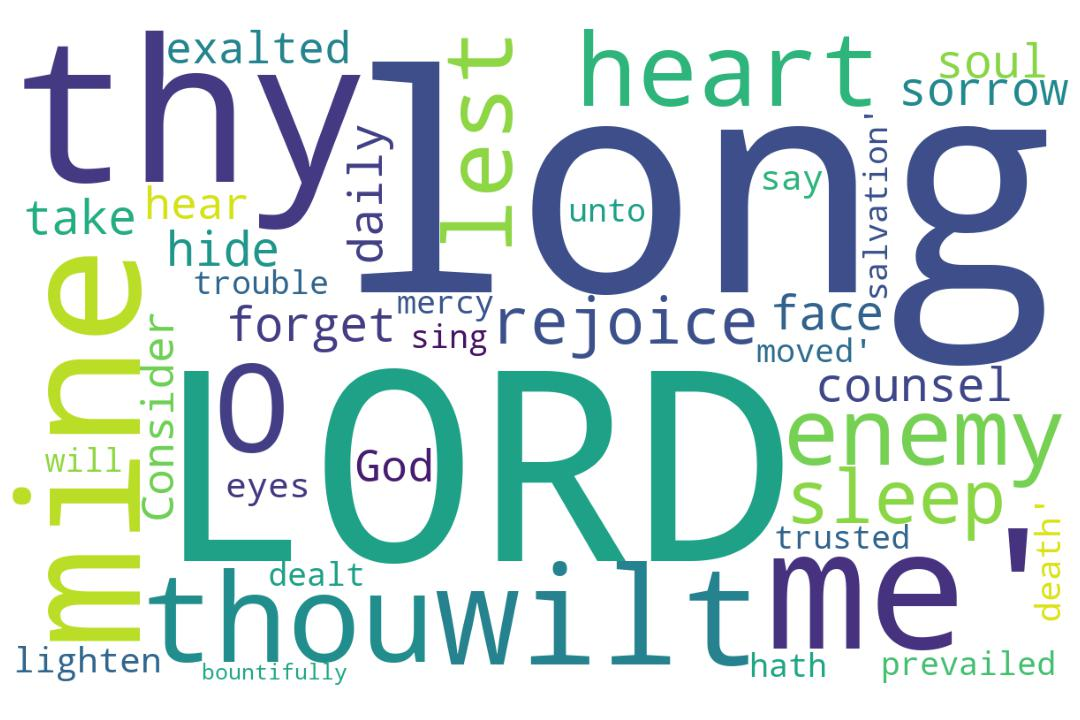
\includegraphics[width=\linewidth]{19OT-Psalms/Psalm13-WordCloud.jpg}
  \caption{Psalm 13 Word Cloud}
  \label{fig:Psalm 13 word Cloud}
\end{figure}


\marginpar{\scriptsize \centering \fcolorbox{bone}{lime}{\textbf{DAVID'S CONTEMPLATION}}\\ (Psalm 13:1-8) 
\begin{compactenum}[I.]
    \item David \textbf{Complains to God} \index[scripture]{Psalms!Psa 013:01}(Psa 13:1)
    \item David \textbf{Confides to God} 
    \item David \textbf{Counsels his Soul}   \index[scripture]{Psalms!Psa 013:02}(Psa 13:2)    
    \item David \textbf{Asks God to Consider him}   \index[scripture]{Psalms!Psa 013:03}(Psa 13:3)
    \item David \textbf{Compares Himself and his Enemies} \index[scripture]{Psalms!Psa 013:04}(Psa 13:4)
    \item David \textbf{Expresses Confidence in God}
    \item David \textbf{Becomes Content with God} \index[scripture]{Psalms!Psa 013:05}(Psa 13:5)
    \item David \textbf{Takes Comfort in God}  \index[scripture]{Psalms!Psa 013:05}(Psa 13:5)%    \item David \textbf{Corrects his Misgivings of God}  \index[scripture]{Psalms!Psa 013:06}(Psalm 13:6)
\end{compactenum}}

\marginpar{\scriptsize \centering \fcolorbox{bone}{yellow}{\textbf{A SONG IN THE HEART}}\\ (Psalm 13:1-8) 
\begin{compactenum}[I.]
    \item The \textbf{Soul} \index[scripture]{Psalms!Psa 013:02}(Psa 13:2)%
    \item The \textbf{Sorrows} \index[scripture]{Psalms!Psa 013:02}(Psa 13:2)%
    \item The \textbf{Supplication} \index[scripture]{Psalms!Psa 013:03}(Psa 13:3)%
    \item The \textbf{Salvation}  \index[scripture]{Psalms!Psa 013:05}(Psa 13:5)%
    \item The \textbf{Satisfaction}  \index[scripture]{Psalms!Psa 013:06}(Psa 13:6)%
    \item The \textbf{Songs} \index[scripture]{Psalms!Psa 013:06}(Psa 13:6)%
\end{compactenum}}

\footnote{\textcolor[cmyk]{0.99998,1,0,0}{\hyperlink{TOC}{Return to end of Table of Contents.}}}\footnote{\href{https://www.audioverse.org/english/audiobibles/books/ENGKJV/O/Ps/1}{\textcolor[cmyk]{0.99998,1,0,0}{Psalms Audio}}}\textcolor[cmyk]{0.99998,1,0,0}{To the chief Musician, A Psalm of David.} %\footnote{John Phillips, How Long? How Long? How Long?:\begin{compactenum}[I.][3]\item Sorrow (Psalm 13:1-2)\item Suplication (Psalm 13:3-4)\item Song  (Psalm 13:5-6)\end{compactenum} } 
\textcolor[cmyk]{0.99998,1,0,0}{\fcolorbox{bone}{lime}{How long} wilt thou forget me, O LORD? for ever? how long wilt thou hide thy face from me?}\footnote{\textbf{Deuteronomy 31:17} - Then my anger shall be kindled against them in that day, and I will forsake them, and I will hide my face from them, and they shall be devoured, and many evils and troubles shall befall them; so that they will say in that day, Are not these evils come upon us, because our God is not among us?}\footnote{\textbf{Job 13:24} - Wherefore hidest thou thy face, and holdest me for thine enemy?}
[2] \textcolor[cmyk]{0.99998,1,0,0}{How long shall I take \fcolorbox{bone}{lime}{counsel} in my soul, \emph{having} sorrow in my heart daily? how long shall mine enemy be exalted over me?}
[3] \textcolor[cmyk]{0.99998,1,0,0}{\fcolorbox{bone}{lime}{Consider} \emph{and} hear me, O LORD my God: lighten mine eyes, lest I sleep the \emph{sleep} \emph{of} death;}
[4] \textcolor[cmyk]{0.99998,1,0,0}{\fcolorbox{bone}{lime}{Lest mine enemy} say, I have prevailed against him; \emph{and} those that trouble me rejoice when I am moved.}\footnote{\textbf{Psalm 3:1} -  LORD, how are they increased that trouble me! many are they that rise up against me.}
[5] \textcolor[cmyk]{0.99998,1,0,0}{But I have trusted in thy mercy; my \fcolorbox{bone}{lime}{heart shall rejoice} in thy salvation.}
[6] \textcolor[cmyk]{0.99998,1,0,0}{\fcolorbox{bone}{lime}{I will sing} unto the LORD, because he hath dealt bountifully with me.}\footnote{\textbf{Psalm 116:7} - Return unto thy rest, O my soul; for the LORD hath dealt bountifully with thee.}\footnote{\textbf{Psalm 119;17} - Deal bountifully with thy servant, that I may live, and keep thy word.}\footnote{\textbf{Psalm 142:7} - Bring my soul out of prison, that I may praise thy name: the righteous shall compass me about; for thou shalt deal bountifully with me.}\footnote{\textbf{2 Corinthians 9:6} - But this I say, He which soweth sparingly shall reap also sparingly; and he which soweth bountifully shall reap also bountifully.}




\section{Psalm 13 Comments}

\subsection{Numeric Nuggets}
There are thirteen words in verse 6, which speaks of singing unto the Lord in response to his bountiful mercy and grace. There are 13 unique words in verse 6. Refusal to sing is rebellion, or evidence of no new birth.

\subsection{Psalm 13:2}
This question ``how long?'' is asked 4 times in this Psalm, 19 in Psalms, and 61 times in scripture.\footnote{Ryrie points out that the four-fold repetition of \emph{how long} indicates the extremity of David's misery.} The first of these is in Exodus 10:3, with Moses and Aaron asking Pharaoh how long would Pharaoh refuse to humble himself before God.\footnote{\textbf{Exodus 10:3} - And Moses and Aaron came in unto Pharaoh, and said unto him, Thus saith the LORD God of the Hebrews, How long wilt thou refuse to humble thyself before me? let my people go, that they may serve me.} We ought to be happy that the patience of God is longer than ours.


\subsection{Psalm 13:6}
See the references to ``fire and brimstone'' here and in Ezekiel 38:22, Luke 17:29, Revelation 14:10, 20:10, and 21:8. ``Fire and brimstone'' speaks of judgment.\\
\\
I have on occasion witnessed the phenomenon of a supposed Christian staying silent while hymns were sung in a church, for multiple years.  How can this be? I have a new song in my heart, and even if I could not carry a tune, I would lift my voice!   The saints are always singing in scripture! Consider the references to ``new song'' (there are nine references - the number of fruitfulness): Psalm 33:3, 40:3, 98:1, 144:9, 149:1, Isaiah 42:10, Revelation 5:9, and 14:4).
%\index[NWIV]{19!Psalms!Psa 13:1}\index[AWIP]{How!Psalms!Psa 13:1}\index[AWIP]{long!Psalms!Psa 13:1}\index[AWIP]{long!Psalms!Psa 13:1 (2)}\index[AWIP]{wilt!Psalms!Psa 13:1}\index[AWIP]{wilt!Psalms!Psa 13:1 (2)}\index[AWIP]{thou!Psalms!Psa 13:1}\index[AWIP]{thou!Psalms!Psa 13:1 (2)}\index[AWIP]{forget!Psalms!Psa 13:1}\index[AWIP]{me!Psalms!Psa 13:1}\index[AWIP]{O!Psalms!Psa 13:1}\index[AWIP]{LORD?!Psalms!Psa 13:1}\index[AWIP]{for!Psalms!Psa 13:1}\index[AWIP]{ever?!Psalms!Psa 13:1}\index[AWIP]{how!Psalms!Psa 13:1}\index[AWIP]{hide!Psalms!Psa 13:1}\index[AWIP]{thy!Psalms!Psa 13:1}\index[AWIP]{face!Psalms!Psa 13:1}\index[AWIP]{from!Psalms!Psa 13:1}\index[AWIP]{me?!Psalms!Psa 13:1}

\index[NWIV]{24!Psalms!Psa 13:2}\index[AWIP]{How!Psalms!Psa 13:2}\index[AWIP]{long!Psalms!Psa 13:2}\index[AWIP]{long!Psalms!Psa 13:2 (2)}\index[AWIP]{shall!Psalms!Psa 13:2}\index[AWIP]{shall!Psalms!Psa 13:2 (2)}\index[AWIP]{I!Psalms!Psa 13:2}\index[AWIP]{take!Psalms!Psa 13:2}\index[AWIP]{counsel!Psalms!Psa 13:2}\index[AWIP]{in!Psalms!Psa 13:2}\index[AWIP]{in!Psalms!Psa 13:2 (2)}\index[AWIP]{my!Psalms!Psa 13:2}\index[AWIP]{my!Psalms!Psa 13:2 (2)}\index[AWIP]{soul!Psalms!Psa 13:2}\index[AWIP]{\emph{having}!Psalms!Psa 13:2}\index[AWIP]{sorrow!Psalms!Psa 13:2}\index[AWIP]{heart!Psalms!Psa 13:2}\index[AWIP]{daily?!Psalms!Psa 13:2}\index[AWIP]{how!Psalms!Psa 13:2}\index[AWIP]{mine!Psalms!Psa 13:2}\index[AWIP]{enemy!Psalms!Psa 13:2}\index[AWIP]{be!Psalms!Psa 13:2}\index[AWIP]{exalted!Psalms!Psa 13:2}\index[AWIP]{over!Psalms!Psa 13:2}\index[AWIP]{me?!Psalms!Psa 13:2}\index[AWIP]{\emph{having}!Psalms!Psa 13:2}

\index[NWIV]{18!Psalms!Psa 13:3}\index[AWIP]{Consider!Psalms!Psa 13:3}\index[AWIP]{\emph{and}!Psalms!Psa 13:3}\index[AWIP]{hear!Psalms!Psa 13:3}\index[AWIP]{me!Psalms!Psa 13:3}\index[AWIP]{O!Psalms!Psa 13:3}\index[AWIP]{LORD!Psalms!Psa 13:3}\index[AWIP]{my!Psalms!Psa 13:3}\index[AWIP]{God!Psalms!Psa 13:3}\index[AWIP]{lighten!Psalms!Psa 13:3}\index[AWIP]{mine!Psalms!Psa 13:3}\index[AWIP]{eyes!Psalms!Psa 13:3}\index[AWIP]{lest!Psalms!Psa 13:3}\index[AWIP]{I!Psalms!Psa 13:3}\index[AWIP]{sleep!Psalms!Psa 13:3}\index[AWIP]{the!Psalms!Psa 13:3}\index[AWIP]{\emph{sleep}!Psalms!Psa 13:3}\index[AWIP]{\emph{of}!Psalms!Psa 13:3}\index[AWIP]{death!Psalms!Psa 13:3}\index[AWIP]{\emph{and}!Psalms!Psa 13:3}\index[AWIP]{\emph{sleep}!Psalms!Psa 13:3}\index[AWIP]{\emph{of}!Psalms!Psa 13:3}

\index[NWIV]{19!Psalms!Psa 13:4}\index[AWIP]{Lest!Psalms!Psa 13:4}\index[AWIP]{mine!Psalms!Psa 13:4}\index[AWIP]{enemy!Psalms!Psa 13:4}\index[AWIP]{say!Psalms!Psa 13:4}\index[AWIP]{I!Psalms!Psa 13:4}\index[AWIP]{I!Psalms!Psa 13:4 (2)}\index[AWIP]{have!Psalms!Psa 13:4}\index[AWIP]{prevailed!Psalms!Psa 13:4}\index[AWIP]{against!Psalms!Psa 13:4}\index[AWIP]{him!Psalms!Psa 13:4}\index[AWIP]{\emph{and}!Psalms!Psa 13:4}\index[AWIP]{those!Psalms!Psa 13:4}\index[AWIP]{that!Psalms!Psa 13:4}\index[AWIP]{trouble!Psalms!Psa 13:4}\index[AWIP]{me!Psalms!Psa 13:4}\index[AWIP]{rejoice!Psalms!Psa 13:4}\index[AWIP]{when!Psalms!Psa 13:4}\index[AWIP]{am!Psalms!Psa 13:4}\index[AWIP]{moved!Psalms!Psa 13:4}\index[AWIP]{\emph{and}!Psalms!Psa 13:4}

\index[NWIV]{14!Psalms!Psa 13:5}\index[AWIP]{But!Psalms!Psa 13:5}\index[AWIP]{I!Psalms!Psa 13:5}\index[AWIP]{have!Psalms!Psa 13:5}\index[AWIP]{trusted!Psalms!Psa 13:5}\index[AWIP]{in!Psalms!Psa 13:5}\index[AWIP]{in!Psalms!Psa 13:5 (2)}\index[AWIP]{thy!Psalms!Psa 13:5}\index[AWIP]{thy!Psalms!Psa 13:5 (2)}\index[AWIP]{mercy!Psalms!Psa 13:5}\index[AWIP]{my!Psalms!Psa 13:5}\index[AWIP]{heart!Psalms!Psa 13:5}\index[AWIP]{shall!Psalms!Psa 13:5}\index[AWIP]{rejoice!Psalms!Psa 13:5}\index[AWIP]{salvation!Psalms!Psa 13:5}

\index[NWIV]{13!Psalms!Psa 13:6}\index[AWIP]{I!Psalms!Psa 13:6}\index[AWIP]{will!Psalms!Psa 13:6}\index[AWIP]{sing!Psalms!Psa 13:6}\index[AWIP]{unto!Psalms!Psa 13:6}\index[AWIP]{the!Psalms!Psa 13:6}\index[AWIP]{LORD!Psalms!Psa 13:6}\index[AWIP]{because!Psalms!Psa 13:6}\index[AWIP]{he!Psalms!Psa 13:6}\index[AWIP]{hath!Psalms!Psa 13:6}\index[AWIP]{dealt!Psalms!Psa 13:6}\index[AWIP]{bountifully!Psalms!Psa 13:6}\index[AWIP]{with!Psalms!Psa 13:6}\index[AWIP]{me!Psalms!Psa 13:6}


\section{Psalm 13 Outlines}

\subsection{My Outlines}

\subsubsection{David's Contemplation}
\index[speaker]{Keith Anthony!Psalm 013 (David's Contemplation)}
\index[series]{Psalms (Keith Anthony)!Psalm 013 (David's Contemplation)}
\index[date]{unknown!Psalm 013 (David's Contemplation) (Keith Anthony)}
\begin{compactenum}[I.][9]
    \item David \textbf{Complains to God} \index[scripture]{Psalms!Psa 013:01}(Psalm 13:1)
    \item David \textbf{Confides to God} 
    \item David \textbf{Counsels his Soul}   \index[scripture]{Psalms!Psa 013:02}(Psalm 13:2)    
    \item David \textbf{Asks God to Consider him}   \index[scripture]{Psalms!Psa 013:03}(Psalm 13:3)
    \item David \textbf{Compares Himself and his Enemies} \index[scripture]{Psalms!Psa 013:04}(Psalm 13:4)
    \item David \textbf{Expresses Confidence in God}
    \item David \textbf{Becomes Content with God} \index[scripture]{Psalms!Psa 013:05}(Psalm 13:5)
    \item David \textbf{Takes Comfort in God}  \index[scripture]{Psalms!Psa 013:05}(Psalm 13:5)
    \item David \textbf{Corrects his Misgivings of God}  \index[scripture]{Psalms!Psa 013:06}(Psalm 13:6)
\end{compactenum}


\subsubsection{A Song in the Heart}
\index[speaker]{Keith Anthony!Psalm 013 (A Song in the Heart)}
\index[series]{Psalms (Keith Anthony)!Psalm 013 (A Song in the Heart)}
\index[date]{unknown!Psalm 013 (A Song in the Heart) (Keith Anthony)}
\begin{compactenum}[I.][9]    \item The \textbf{Soul} \index[scripture]{Psalms!Psa 013:02}(Psa 13:2)%
    \item The \textbf{Sorrows} \index[scripture]{Psalms!Psa 013:02}(Psa 13:2)%
    \item The \textbf{Supplication} \index[scripture]{Psalms!Psa 013:03}(Psa 13:3)%
    \item The \textbf{Salvation}  \index[scripture]{Psalms!Psa 013:05}(Psa 13:5)%
    \item The \textbf{Satisfaction}  \index[scripture]{Psalms!Psa 013:06}(Psa 13:6)%
    \item The \textbf{Songs} \index[scripture]{Psalms!Psa 013:06}(Psa 13:6)%
\end{compactenum}


\subsection{Outlines from Others}


%\section{Psalm 13 Statistics}

%%%%%%%%%%%%%%%%%%%%%%%%%%%
%%%%%Word Statistics
%%%%%%%%%%%%%%%%%%%%%%%%%%%


\normalsize



\subsection{Chapter Word Statistics}


%%%%%%%%%%
%%%%%%%%%%
 
\begin{center}
\begin{longtable}{l|c|c|c|c}
\caption[Stats for Psalm 13]{Stats for Psalm 13} \label{table:Stats for Psalm 13} \\ 
\hline \multicolumn{1}{|c|}{\textbf{Verse(s)}} & \multicolumn{1}{|c|}{\textbf{Count}} & \multicolumn{1}{|c|}{\textbf{Unique}} & \multicolumn{1}{|c|}{\textbf{Italics}} & \multicolumn{1}{|c|}{\textbf{Uniq Italic}}  \\ \hline 
\endfirsthead
 
\multicolumn{5}{c}
{{\bfseries \tablename\ \thetable{} -- continued from previous page}} \\  
\hline \multicolumn{1}{|c|}{\textbf{Verse(s)}} & \multicolumn{1}{|c|}{\textbf{Count}} & \multicolumn{1}{|c|}{\textbf{Unique}} & \multicolumn{1}{|c|}{\textbf{Italics}} & \multicolumn{1}{|c|}{\textbf{Uniq Italic}}  \\ \hline 
\endhead
 
\hline \multicolumn{5}{|r|}{{Continued if needed}} \\ \hline
\endfoot 
1 & 19 & 15 & 0 & 0\\ \hline
2 & 24 & 20 & 1 & 1\\ \hline
3 & 18 & 18 & 3 & 3\\ \hline
4 & 19 & 18 & 1 & 1\\ \hline
5 & 14 & 12 & 0 & 0\\ \hline
6 & 13 & 13 & 0 & 0\\ \hline
\hline \hline
Total & 107 & 69 & 5 & 4



\end{longtable}
\end{center}

%%%%%%%%%%
%%%%%%%%%%
 
\subsection{Words by Frequency}

\begin{center}
\begin{longtable}{l|r}
\caption[Word Frequencies in Psalm 13]{Word Frequencies in Psalm 13} \label{table:WordsIn-Psalm-13} \\ 
\hline \multicolumn{1}{|c|}{\textbf{Word}} & \multicolumn{1}{c|}{\textbf{Frequency}} \\ \hline 
\endfirsthead
 
\multicolumn{2}{c}
{{\bfseries \tablename\ \thetable{} -- continued from previous page}} \\ 
\hline \multicolumn{1}{|c|}{\textbf{Word}} & \multicolumn{1}{c|}{\textbf{Frequency}} \\ \hline 
\endhead
 
\hline \multicolumn{2}{|r|}{{Continued if needed}} \\ \hline
\endfoot
 
\hline \hline
\endlastfoot
me & 6 \\ \hline
I & 6 \\ \hline
long & 4 \\ \hline
in & 4 \\ \hline
my & 4 \\ \hline
LORD & 3 \\ \hline
thy & 3 \\ \hline
shall & 3 \\ \hline
mine & 3 \\ \hline
How & 2 \\ \hline
wilt & 2 \\ \hline
thou & 2 \\ \hline
O & 2 \\ \hline
how & 2 \\ \hline
heart & 2 \\ \hline
enemy & 2 \\ \hline
\emph{and} & 2 \\ \hline
the & 2 \\ \hline
have & 2 \\ \hline
rejoice & 2 \\ \hline
forget & 1 \\ \hline
for & 1 \\ \hline
ever & 1 \\ \hline
hide & 1 \\ \hline
face & 1 \\ \hline
from & 1 \\ \hline
take & 1 \\ \hline
counsel & 1 \\ \hline
soul & 1 \\ \hline
\emph{having} & 1 \\ \hline
sorrow & 1 \\ \hline
daily & 1 \\ \hline
be & 1 \\ \hline
exalted & 1 \\ \hline
over & 1 \\ \hline
Consider & 1 \\ \hline
hear & 1 \\ \hline
God & 1 \\ \hline
lighten & 1 \\ \hline
eyes & 1 \\ \hline
lest & 1 \\ \hline
sleep & 1 \\ \hline
\emph{sleep} & 1 \\ \hline
\emph{of} & 1 \\ \hline
death & 1 \\ \hline
Lest & 1 \\ \hline
say & 1 \\ \hline
prevailed & 1 \\ \hline
against & 1 \\ \hline
him & 1 \\ \hline
those & 1 \\ \hline
that & 1 \\ \hline
trouble & 1 \\ \hline
when & 1 \\ \hline
am & 1 \\ \hline
moved & 1 \\ \hline
But & 1 \\ \hline
trusted & 1 \\ \hline
mercy & 1 \\ \hline
salvation & 1 \\ \hline
will & 1 \\ \hline
sing & 1 \\ \hline
unto & 1 \\ \hline
because & 1 \\ \hline
he & 1 \\ \hline
hath & 1 \\ \hline
dealt & 1 \\ \hline
bountifully & 1 \\ \hline
with & 1 \\ \hline
\end{longtable}
\end{center}



\normalsize



\subsection{Words Alphabetically}

\begin{center}
\begin{longtable}{l|r}
\caption[Word Alphabetically in Psalm 13]{Word Alphabetically in Psalm 13} \label{table:WordsIn-Psalm-13} \\ 
\hline \multicolumn{1}{|c|}{\textbf{Word}} & \multicolumn{1}{c|}{\textbf{Frequency}} \\ \hline 
\endfirsthead
 
\multicolumn{2}{c}
{{\bfseries \tablename\ \thetable{} -- continued from previous page}} \\ 
\hline \multicolumn{1}{|c|}{\textbf{Word}} & \multicolumn{1}{c|}{\textbf{Frequency}} \\ \hline 
\endhead
 
\hline \multicolumn{2}{|r|}{{Continued if needed}} \\ \hline
\endfoot
 
\hline \hline
\endlastfoot
But & 1 \\ \hline
Consider & 1 \\ \hline
God & 1 \\ \hline
How & 2 \\ \hline
I & 6 \\ \hline
LORD & 3 \\ \hline
Lest & 1 \\ \hline
O & 2 \\ \hline
\emph{and} & 2 \\ \hline
\emph{having} & 1 \\ \hline
\emph{of} & 1 \\ \hline
\emph{sleep} & 1 \\ \hline
against & 1 \\ \hline
am & 1 \\ \hline
be & 1 \\ \hline
because & 1 \\ \hline
bountifully & 1 \\ \hline
counsel & 1 \\ \hline
daily & 1 \\ \hline
dealt & 1 \\ \hline
death & 1 \\ \hline
enemy & 2 \\ \hline
ever & 1 \\ \hline
exalted & 1 \\ \hline
eyes & 1 \\ \hline
face & 1 \\ \hline
for & 1 \\ \hline
forget & 1 \\ \hline
from & 1 \\ \hline
hath & 1 \\ \hline
have & 2 \\ \hline
he & 1 \\ \hline
hear & 1 \\ \hline
heart & 2 \\ \hline
hide & 1 \\ \hline
him & 1 \\ \hline
how & 2 \\ \hline
in & 4 \\ \hline
lest & 1 \\ \hline
lighten & 1 \\ \hline
long & 4 \\ \hline
me & 6 \\ \hline
mercy & 1 \\ \hline
mine & 3 \\ \hline
moved & 1 \\ \hline
my & 4 \\ \hline
over & 1 \\ \hline
prevailed & 1 \\ \hline
rejoice & 2 \\ \hline
salvation & 1 \\ \hline
say & 1 \\ \hline
shall & 3 \\ \hline
sing & 1 \\ \hline
sleep & 1 \\ \hline
sorrow & 1 \\ \hline
soul & 1 \\ \hline
take & 1 \\ \hline
that & 1 \\ \hline
the & 2 \\ \hline
those & 1 \\ \hline
thou & 2 \\ \hline
thy & 3 \\ \hline
trouble & 1 \\ \hline
trusted & 1 \\ \hline
unto & 1 \\ \hline
when & 1 \\ \hline
will & 1 \\ \hline
wilt & 2 \\ \hline
with & 1 \\ \hline
\end{longtable}
\end{center}



\normalsize



\subsection{Word Lengths in Chapter}
\normalsize
\begin{longtable}{l|p{3.75in}}
\caption[Words by Length in Psalm 13]{Words by Length in Psalm 13} \label{table:WordsIn-Psalm-13} \\ 
\hline \multicolumn{1}{|c|}{\textbf{Length}} & \multicolumn{1}{c|}{\textbf{Words}} \\ \hline 
\endfirsthead
 
\multicolumn{2}{c}
{{\bfseries \tablename\ \thetable{} -- continued from previous page}} \\ 
\hline \multicolumn{1}{|c|}{\textbf{Length}} & \multicolumn{1}{c|}{\textbf{Words}} \\ \hline 
\endhead
 
\hline \multicolumn{2}{|r|}{{Continued if needed}} \\ \hline
\endfoot
 
\hline \hline
\endlastfoot
1 & O, I \\ \hline
2 & me, in, my, be, \emph{of}, am, he \\ \hline
3 & How, for, how, thy, \emph{and}, God, the, say, him, But \\ \hline
4 & long, wilt, thou, LORD, ever, hide, face, from, take, soul, mine, over, hear, eyes, lest, Lest, have, that, when, will, sing, unto, hath, with \\ \hline
5 & shall, heart, daily, enemy, sleep, \emph{sleep}, death, those, moved, mercy, dealt \\ \hline
6 & forget, \emph{having}, sorrow \\ \hline
7 & counsel, exalted, lighten, against, trouble, rejoice, trusted, because \\ \hline
8 & Consider \\ \hline
9 & prevailed, salvation \\ \hline
11 & bountifully \\ \hline
\end{longtable}






%%%%%%%%%%
%%%%%%%%%%
 



%%%%%%%%%%
%%%%%%%%%%
\subsection{Verses with 13 Words in Chapter}
\normalsize
\begin{longtable}{l|p{3.75in}}
\caption[Verses with 13 Words  in Psalm 13]{Verses with 13 Words  in Psalm 13} \label{table:Verses with 13 Words in-Psalm-13} \\ 
\hline \multicolumn{1}{|c|}{\textbf{Reference}} & \multicolumn{1}{c|}{\textbf{Verse}} \\ \hline 
\endfirsthead
 
\multicolumn{2}{c}
{{\bfseries \tablename\ \thetable{} -- continued from previous page}} \\ 
\hline \multicolumn{1}{|c|}{\textbf{Reference}} & \multicolumn{1}{c|}{\textbf{Verse}} \\ \hline 
\endhead
 
\hline \multicolumn{2}{|r|}{{Continued if needed}} \\ \hline
\endfoot
 
\hline \hline
\endlastfoot
Psalms 13:6 & I will sing unto the LORD, because he hath dealt bountifully with me. \\ \hline
\end{longtable}






%%%%%%%%%%
%%%%%%%%%%
 



%%%%%%%%%%
%%%%%%%%%%
\subsection{Verses with 18 Words in Chapter}
\normalsize
\begin{longtable}{l|p{3.75in}}
\caption[Verses with 18 Words  in Psalm 13]{Verses with 18 Words  in Psalm 13} \label{table:Verses with 18 Words in-Psalm-13} \\ 
\hline \multicolumn{1}{|c|}{\textbf{Reference}} & \multicolumn{1}{c|}{\textbf{Verse}} \\ \hline 
\endfirsthead
 
\multicolumn{2}{c}
{{\bfseries \tablename\ \thetable{} -- continued from previous page}} \\ 
\hline \multicolumn{1}{|c|}{\textbf{Reference}} & \multicolumn{1}{c|}{\textbf{Verse}} \\ \hline 
\endhead
 
\hline \multicolumn{2}{|r|}{{Continued if needed}} \\ \hline
\endfoot
 
\hline \hline
\endlastfoot
Psalms 13:3 & Consider \emph{and} hear me, O LORD my God: lighten mine eyes, lest I sleep the \emph{sleep} \emph{of} death; \\ \hline
\end{longtable}






%%%%%%%%%%
%%%%%%%%%%
\subsection{Psalm 13 Repeated Phrases}


%%%%%%%%%%
%%%%%%%%%%
\normalsize
 
\begin{center}
\begin{longtable}{|p{3.0in}|p{0.5in}|}
\caption[Psalm 13 Repeated Phrases]{Psalm 13 Repeated Phrases}\label{table:Repeated Phrases Psalm 13} \\
\hline \multicolumn{1}{|c|}{\textbf{Phrase}} & \multicolumn{1}{c|}{\textbf{Frequency}} \\ \hline 
\endfirsthead
 
\multicolumn{2}{c}
{{\bfseries \tablename\ \thetable{} -- continued from previous page}} \\  
\hline \multicolumn{1}{|c|}{\textbf{Phrase}} & \multicolumn{1}{c|}{\textbf{Frequency}} \\ \hline 
\endhead
 
\hline \multicolumn{2}{c}{{ }} \\ \hline
\endfoot 
\end{longtable}
\end{center}



%%%%%%%%%%
%%%%%%%%%%




\chapter{Psalm 14}

\begin{figure}
  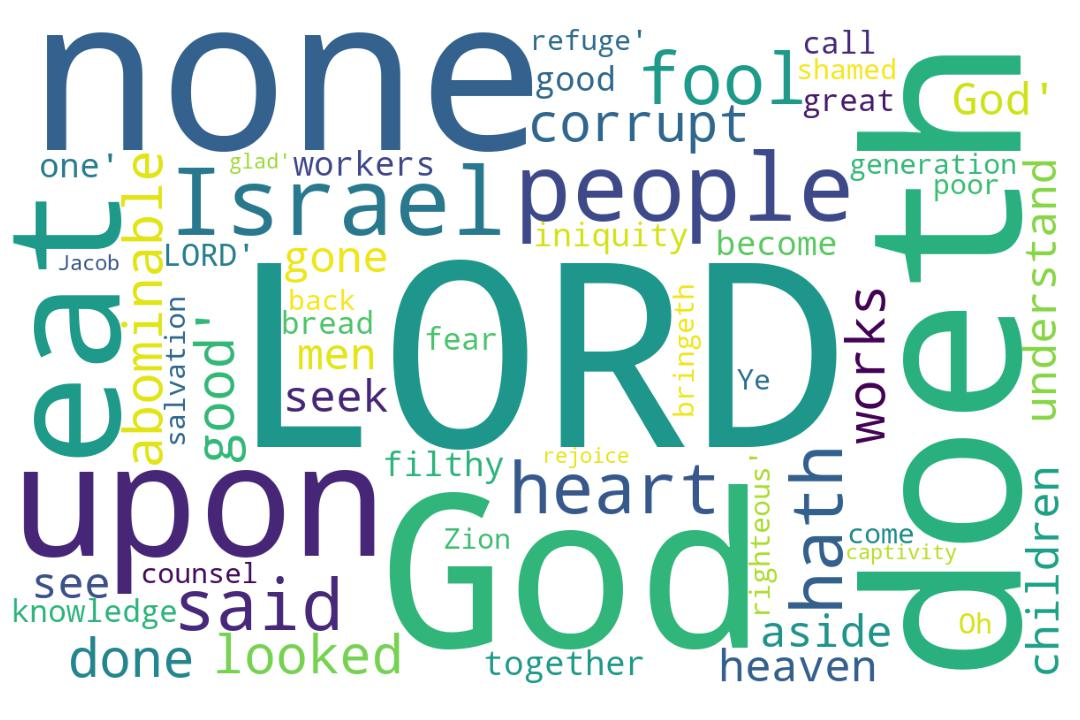
\includegraphics[width=\linewidth]{19OT-Psalms/Psalm14-WordCloud.jpg}
  \caption{Psalm 14 Word Cloud}
  \label{fig:Psalm 14 word Cloud}
\end{figure}



\marginpar{\scriptsize \centering \fcolorbox{bone}{lime}{\textbf{THINGS OF THE WICKED}}\\ (Psalm 14:1-7) \begin{compactenum}[I.][8]
    \item \textbf{Dwelling Place} of the Wicked (Job 08:22) 
	\item\textbf{Foolish Atheists} - They say this because they choose to believe it, as if saying so will make God disappear. It is like the ostrich burying his head in sand - if they can't see God, or won't, then God will go away for them. (Psa 14:1) 
	\item  \textbf{Full Abandonement}  (Psa 14:3)
	\item Man has become \textbf{Filthy Altogether} (Psa 14:3)
	\item Man has developed a \textbf{Fierce Appetite} (Psa 14:4)
	\item But they have a \textbf{Fearful Attitude} (Psa 14:5)
    \item David awaits the \textbf{Final Arrival} (Psa 14:7)
\end{compactenum}}

\marginpar{\scriptsize \centering \fcolorbox{bone}{yellow}{\textbf{LANGUISHING AND LONGING}}\\ (Psalm 14:1-7) \begin{compactenum}[I.][8]
    \item \textbf{Foul Activities} (Psa 14:1) 
	\item\textbf{Foolish Atheists} - They say this because they choose to believe it, as if saying so will make God disappear. It is like the ostrich burying his head in sand - if they can't see God, or won't, then God will go away for them. (Psa 14:1) 
	\item  \textbf{Full Abandonement}  (Psa 14:3)
	\item Man has become \textbf{Filthy Altogether} (Psa 14:3)
	\item Man has developed a \textbf{Fierce Appetite} (Psa 14:4)
	\item But they have a \textbf{Fearful Attitude} (Psa 14:5)
    \item David awaits the \textbf{Final Arrival} (Psa 14:7)
\end{compactenum}}

\footnote{\textcolor[cmyk]{0.99998,1,0,0}{\hyperlink{TOC}{Return to end of Table of Contents.}}}\footnote{\href{https://www.audioverse.org/english/audiobibles/books/ENGKJV/O/Ps/1}{\textcolor[cmyk]{0.99998,1,0,0}{Psalms Audio}}}\textcolor[cmyk]{0.99998,1,0,0}{To the chief Musician, \emph{A Psalm} of David.}\footnote{Ryrie notes that this psalm, with only slight changes in verse 5 and 6, is identical to Psalm 53. \cite{ryrie2008ryrieKJV}
\begin{compactenum}[I.][3]
\item (Psalm 14:1-6) David laments the moral foolishness and corruption of the whole human race  
\item (Psalm 14:7) David  longs for the establishment of the righteous kingdom of the Lord of earth (14:7)
\end{compactenum} }\\
\\
\textcolor[cmyk]{0.99998,1,0,0}{The fool hath said in his heart, \emph{There} \emph{is} no God. They are corrupt, they have done abominable works, \emph{there} \emph{is} none that doeth good.}\footnote{From Kidner, the spirit of godlessness reveals itself in two ways:  in flouting God's law (1-3) and oppressing His people (4-6); that is, in both direct and indirect contempt of heaven. It is the reckless folly (1a,2b, 4a) almost as much as the wickedness of it that energes in the psalm, which `looks down from heaven' on the scene as God views it. But the standpoint changes in the last verse to the earthly arena, where persecuted Israel waits longingly for the redress that will surely come. The psalm is almost exactly duplicated in Psalm 53, where, however, the term `God' replaces `The Lord'. \cite{kidner2014psalmsV1} } 
[2] \textcolor[cmyk]{0.99998,1,0,0}{The LORD looked down from heaven upon the children of men, to see if there were any that did understand, \emph{and} seek God.}\footnote{\textbf{Psalm 11:4} - The LORD is in his holy temple, the LORD'S throne is in heaven: his eyes behold, his eyelids try, the children of men.}\footnote{\textbf{Psalm 33:13} - The LORD looketh from heaven; he beholdeth all the sons of men.}\footnote{\textbf{Psalm 102:19} - For he hath looked down from the height of his sanctuary; from heaven did the LORD behold the earth;}
[3] \textcolor[cmyk]{0.99998,1,0,0}{They are all gone aside, they are \emph{all} together become filthy: \emph{there} \emph{is} none that doeth good, no, not one.}\footnote{\textbf{Romans 3:10-12} - }
[4] \textcolor[cmyk]{0.99998,1,0,0}{Have all the workers of iniquity no knowledge? who eat up my people \emph{as} they eat bread, and call not upon the LORD.}%\footnote{These are the people that say you cannot correct “the Hebrew’’ with the English. These are the people who swear by ``plenary, verbally inspired'' scraps of paper that contain a DEAD language on them. These are the people that would call you a ``heretic'' for correcting their banal, benighted, bewildered, tedious, misinformed BUNKO with the Authorized Version. Had enough? Ready for some Scripture instead of the ``original Hebrew''? \begin{compactenum}
%\item People in the Bible EAT people (Lam. 4:10; Deut. 28:53–56; 2 Kings 6:29). Is that clear? Do you understand that?
%\item Dragons eat people (Jer. 51:34). Do you understand that?
%\item Israelites will be eaten (Isa. 6:13). Do you understand THAT?
%\item Someone goes after a Jew to eat his flesh (Ps. 27:2).
%\item Someone who professed to drink literal blood every Sunday morning at eleven o’clock, offers drink offerings of blood (Ps. 16:4). Any trouble yet?
%\item When you sacrifice at an altar, you cut off the head of the victim (Lev. 1:12). When you sacrifice people (Rev. 6:9) you cut off their heads (Rev. 20:4). Any problem? What is the problem?
%\end{compactenum} }
\footnote{\textbf{Psalm 27:2} -- When the wicked, even mine enemies and my foes, came upon me to eat up my flesh, they stumbled and fell.}
[5] \textcolor[cmyk]{0.99998,1,0,0}{There were they in great fear: for God \emph{is} in the generation of the righteous.}
[6] \textcolor[cmyk]{0.99998,1,0,0}{Ye have shamed the counsel of the poor, because the LORD \emph{is} his refuge.}\footnote{\textbf{Psalm 9:9} - The LORD also will be a refuge for the oppressed, a refuge in times of trouble.}\footnote{\textbf{Hebrews 6:18} - That by two immutable things, in which it was impossible for God to lie, we might have a strong consolation, who have fled for refuge to lay hold upon the hope set before us:}\footnote{\textbf{Psalm 22:30} -- A seed shall serve him; it shall be accounted to the Lord for a generation.}\footnote{\textbf{Psalm 24:6} - This is the generation of them that seek him, that seek thy face, O Jacob. Selah.}\footnote{\textbf{PSalm 73:15} - If I say, I will speak thus; behold, I should offend against the generation of thy children.}\footnote{\textbf{Psalm 112:2} - His seed shall be mighty upon earth: the generation of the upright shall be blessed.}\footnote{\textbf{1 Peter 2:9} - But ye are a chosen generation, a royal priesthood, an holy nation, a peculiar people; that ye should shew forth the praises of him who hath called you out of darkness into his marvellous light:}
[7] \textcolor[cmyk]{0.99998,1,0,0}{Oh that the salvation of Israel \emph{were} \emph{come} out of Zion! when the LORD bringeth back the captivity of his people, Jacob shall rejoice, \emph{and} Israel shall be glad.}\footnote{\textbf{Psalm 53:6} - Oh that the salvation of Israel were come out of Zion! When God bringeth back the captivity of his people, Jacob shall rejoice, and Israel shall be glad.}

\section{Psalm 14 Comments}

\subsection{NUmeric Nuggets}
\textbf{13:} Verse 5 has 13 unique words.

\subsection{Psalm 14:3}

\begin{center}

\begin{table}[ht]
\centering
\begin{tabular}{|p{.5in}|p{3.5in}|}
    \hline

\textcolor[rgb]{0.00,0.00,1.00}{AV} & \textcolor[rgb]{0.00,0.00,1.00}{They are all gone aside, they are all together become filthy: there is none that doeth good, no, not one.} \\ \hline
%%
ASV & They are all gone aside; they are together become filthy;
There is none that doeth good, no, not one.\\ \hline
%
CEB &  but all of them have turned bad. Everyone is corrupt. No one does good -- not even one person!\\ \hline
%&
ESV & They have all turned aside; together they have become corrupt; there is none who does good, not even one.\\ \hline
%
NASV &  They have all turned aside, together they have become corrupt; There is no one who does good, not even one.\\ \hline
%
MEV & They all turn aside, together they become corrupt; there is none who does good, not even one. \\ \hline
%
NIV & All have turned away, all have become corrupt;  there is no one who does good,  not even one. \\ \hline
%
NKJV &  They have all turned aside, They have together become corrupt; \emph{There is} none who does good, No, not one.\\ \hline
%
RSV &   They have all gone astray, they are all alike corrupt; there is none that does good,  no, not one.\\ \hline

\multicolumn{2}{p{4.0in}}{{To start off with, here are Origen and his buddies sitting down in A.D. 200 and adding Romans 3:13 to Psalm 14:4 verbatim. After this, the stupid ``godly'' scholars pretend that Paul was reading a Greek Old Testament written more than one hundred years after he was dead.  Verse 3 in the LXX says, ``Their throat is an open sepulchre, with their tongues they have used deceit; the poison of asps ....''  The writer of this verse in the Psalms wrote it in A.D. 330 and copied it directly out of the New Testament into the Old Testament, thus adding to all of the Hebrew texts. To this day, every professor on the staff of every major Christian school in the world believes that Paul quoted a manuscript written AFTER the Council of Nicaea.\cite{Ruckman1992psalms}}} \\ \end{tabular}

\caption[Corruption Alert: Psalm 10:2]{Corruption Alert: Psalm 10:2} \label{table:Corruption Psalm 10:2}
\end{table}

\end{center}



%\hline \multicolumn{2}{|r|}{{Continued on next page}} \\ \hline
%\endfoot 
%\textcolor[rgb]{0.00,0.00,1.00}{AV} & \textcolor[rgb]{0.00,0.00,1.00}{They are all gone aside, they are all together %become filthy: there is none that doeth good, no, not one.}\\ \hline
%CEB &  but all of them have turned bad. Everyone is corrupt. No one does good -- not even one person!\\ \hline
%ESV &They have all turned aside; together they have become corrupt; there is none who does good, not even one. \\ \hline
%NASV &  They have all turned aside, together they have become corrupt; There is no one who does good, not even one.\\ \hline
%MEV & They all turn aside, together they become corrupt; there is none who does good, not even one.\\ \hline
%NIV &  All have turned away, all have become corrupt;  there is no one who does good,  not even one.\\ \hline
%NKJV &  They have all turned aside, They have together become corrupt; \emph{There is} none who does good, No, not one. \\ \hline
%RSV &  They have all gone astray, t

%%%%%%EXAMPLE Corruption Table
%\newpage
%\begin{mdframed}[style=MyFrame]
%\begin{center}
%\begin{longtable}{|p{.5in}|p{3.5in}|}

%\caption[Corruption Alert: Psalm 14:3]{Corruption Alert: Psalm 14:3} \label{table:CorruptionPsalm014003} \\ 

%\hline  
%\multicolumn{1}{|c|}{\textbf{Version}} & 
%\multicolumn{1}{c|}{\textbf{Corruption}}  \\ \hline 
%\endfirsthead
 
%\multicolumn{2}{c}
%{{\bfseries \tablename\ \thetable{} -- continued from previous page}} \%\  \hline  
%\multicolumn{1}{|c|}{\textbf{Version}} & 
%\multicolumn{1}{c|}{\textbf{Corruption}}  \\ \hline 
%\endhead
 
%\hline \multicolumn{2}{|r|}{{Continued on next page}} \\ \hline
%\endfoot 
%\textcolor[rgb]{0.00,0.00,1.00}{AV} & \textcolor[rgb]{0.00,0.00,1.00}{They are all gone aside, they are all together %become filthy: there is none that doeth good, no, not one.}\\ \hline
%CEB &  but all of them have turned bad. Everyone is corrupt. No one does good -- not even one person!\\ \hline
%ESV &They have all turned aside; together they have become corrupt;
%there is none who does good, not even one. \\ \hline
%NASV &  They have all turned aside, together they have become corrupt;
%There is no one who does good, not even one.\\ \hline
%MEV & They all turn aside, together they become corrupt;
%there is none who does good, not even one.\\ \hline
%NIV &  All have turned away, all have become corrupt;  there is no one who does good,  not even one.\\ \hline
%NKJV &  They have all turned aside, They have together become corrupt;
%\emph{There is} none who does good, No, not one. \\ \hline
%RSV &  They have all gone astray, they are all alike corrupt; there is none that does good,  no, not one. \\ %\hline

% \multicolumn{2}{p{4.0in}}{{To start off with, here are Origen and his buddies sitting down in A.D. 200 and adding %Romans 3:13 to Psalm 14:4 verbatim. After this, the stupid “godly” scholars pretend that Paul was reading a Greek Old %Testament written more than one hundred years after he was dead.  Verse 3 in the LXX says, “Their throat is an open %sepulchre, with their tongues they have used deceit; the poison of asps....”  The writer of this verse in the Psalms %wrote it in A.D. 330 and copied it directly out of the New Testament into the Old Testament, thus adding to all of the %Hebrew texts. To this day, every professor on the staff of every major Christian school in the world believes that Paul %quoted a manuscript written AFTER the Council of Nicaea.\cite{Ruckman1992psalms}}} \\ %\hline

%\hline

%\end{longtable}
%\end{center}

%\normalsize 
%\end{mdframed}
%\index[NWIV]{25!Psalms!Psa 14:1}\index[AWIP]{The!Psalms!Psa 14:1}\index[AWIP]{fool!Psalms!Psa 14:1}\index[AWIP]{hath!Psalms!Psa 14:1}\index[AWIP]{said!Psalms!Psa 14:1}\index[AWIP]{in!Psalms!Psa 14:1}\index[AWIP]{his!Psalms!Psa 14:1}\index[AWIP]{heart!Psalms!Psa 14:1}\index[AWIP]{\emph{There}!Psalms!Psa 14:1}\index[AWIP]{\emph{is}!Psalms!Psa 14:1}\index[AWIP]{\emph{is}!Psalms!Psa 14:1 (2)}\index[AWIP]{no!Psalms!Psa 14:1}\index[AWIP]{God!Psalms!Psa 14:1}\index[AWIP]{They!Psalms!Psa 14:1}\index[AWIP]{are!Psalms!Psa 14:1}\index[AWIP]{corrupt!Psalms!Psa 14:1}\index[AWIP]{they!Psalms!Psa 14:1}\index[AWIP]{have!Psalms!Psa 14:1}\index[AWIP]{done!Psalms!Psa 14:1}\index[AWIP]{abominable!Psalms!Psa 14:1}\index[AWIP]{works!Psalms!Psa 14:1}\index[AWIP]{\emph{there}!Psalms!Psa 14:1}\index[AWIP]{none!Psalms!Psa 14:1}\index[AWIP]{that!Psalms!Psa 14:1}\index[AWIP]{doeth!Psalms!Psa 14:1}\index[AWIP]{good!Psalms!Psa 14:1}\index[AWIP]{\emph{There}!Psalms!Psa 14:1}\index[AWIP]{\emph{is}!Psalms!Psa 14:1}\index[AWIP]{\emph{is}!Psalms!Psa 14:1 (2)}\index[AWIP]{\emph{there}!Psalms!Psa 14:1}

\index[NWIV]{23!Psalms!Psa 14:2}\index[AWIP]{The!Psalms!Psa 14:2}\index[AWIP]{LORD!Psalms!Psa 14:2}\index[AWIP]{looked!Psalms!Psa 14:2}\index[AWIP]{down!Psalms!Psa 14:2}\index[AWIP]{from!Psalms!Psa 14:2}\index[AWIP]{heaven!Psalms!Psa 14:2}\index[AWIP]{upon!Psalms!Psa 14:2}\index[AWIP]{the!Psalms!Psa 14:2}\index[AWIP]{children!Psalms!Psa 14:2}\index[AWIP]{of!Psalms!Psa 14:2}\index[AWIP]{men!Psalms!Psa 14:2}\index[AWIP]{to!Psalms!Psa 14:2}\index[AWIP]{see!Psalms!Psa 14:2}\index[AWIP]{if!Psalms!Psa 14:2}\index[AWIP]{there!Psalms!Psa 14:2}\index[AWIP]{were!Psalms!Psa 14:2}\index[AWIP]{any!Psalms!Psa 14:2}\index[AWIP]{that!Psalms!Psa 14:2}\index[AWIP]{did!Psalms!Psa 14:2}\index[AWIP]{understand!Psalms!Psa 14:2}\index[AWIP]{\emph{and}!Psalms!Psa 14:2}\index[AWIP]{seek!Psalms!Psa 14:2}\index[AWIP]{God!Psalms!Psa 14:2}\index[AWIP]{\emph{and}!Psalms!Psa 14:2}

\index[NWIV]{20!Psalms!Psa 14:3}\index[AWIP]{They!Psalms!Psa 14:3}\index[AWIP]{are!Psalms!Psa 14:3}\index[AWIP]{are!Psalms!Psa 14:3 (2)}\index[AWIP]{all!Psalms!Psa 14:3}\index[AWIP]{gone!Psalms!Psa 14:3}\index[AWIP]{aside!Psalms!Psa 14:3}\index[AWIP]{they!Psalms!Psa 14:3}\index[AWIP]{\emph{all}!Psalms!Psa 14:3}\index[AWIP]{together!Psalms!Psa 14:3}\index[AWIP]{become!Psalms!Psa 14:3}\index[AWIP]{filthy!Psalms!Psa 14:3}\index[AWIP]{\emph{there}!Psalms!Psa 14:3}\index[AWIP]{\emph{is}!Psalms!Psa 14:3}\index[AWIP]{none!Psalms!Psa 14:3}\index[AWIP]{that!Psalms!Psa 14:3}\index[AWIP]{doeth!Psalms!Psa 14:3}\index[AWIP]{good!Psalms!Psa 14:3}\index[AWIP]{no!Psalms!Psa 14:3}\index[AWIP]{not!Psalms!Psa 14:3}\index[AWIP]{one!Psalms!Psa 14:3}\index[AWIP]{\emph{all}!Psalms!Psa 14:3}\index[AWIP]{\emph{there}!Psalms!Psa 14:3}\index[AWIP]{\emph{is}!Psalms!Psa 14:3}

\index[NWIV]{23!Psalms!Psa 14:4}\index[AWIP]{Have!Psalms!Psa 14:4}\index[AWIP]{all!Psalms!Psa 14:4}\index[AWIP]{the!Psalms!Psa 14:4}\index[AWIP]{the!Psalms!Psa 14:4 (2)}\index[AWIP]{workers!Psalms!Psa 14:4}\index[AWIP]{of!Psalms!Psa 14:4}\index[AWIP]{iniquity!Psalms!Psa 14:4}\index[AWIP]{no!Psalms!Psa 14:4}\index[AWIP]{knowledge?!Psalms!Psa 14:4}\index[AWIP]{who!Psalms!Psa 14:4}\index[AWIP]{eat!Psalms!Psa 14:4}\index[AWIP]{eat!Psalms!Psa 14:4 (2)}\index[AWIP]{up!Psalms!Psa 14:4}\index[AWIP]{my!Psalms!Psa 14:4}\index[AWIP]{people!Psalms!Psa 14:4}\index[AWIP]{\emph{as}!Psalms!Psa 14:4}\index[AWIP]{they!Psalms!Psa 14:4}\index[AWIP]{bread!Psalms!Psa 14:4}\index[AWIP]{and!Psalms!Psa 14:4}\index[AWIP]{call!Psalms!Psa 14:4}\index[AWIP]{not!Psalms!Psa 14:4}\index[AWIP]{upon!Psalms!Psa 14:4}\index[AWIP]{LORD!Psalms!Psa 14:4}\index[AWIP]{\emph{as}!Psalms!Psa 14:4}

\index[NWIV]{15!Psalms!Psa 14:5}\index[AWIP]{There!Psalms!Psa 14:5}\index[AWIP]{were!Psalms!Psa 14:5}\index[AWIP]{they!Psalms!Psa 14:5}\index[AWIP]{in!Psalms!Psa 14:5}\index[AWIP]{in!Psalms!Psa 14:5 (2)}\index[AWIP]{great!Psalms!Psa 14:5}\index[AWIP]{fear!Psalms!Psa 14:5}\index[AWIP]{for!Psalms!Psa 14:5}\index[AWIP]{God!Psalms!Psa 14:5}\index[AWIP]{\emph{is}!Psalms!Psa 14:5}\index[AWIP]{the!Psalms!Psa 14:5}\index[AWIP]{the!Psalms!Psa 14:5 (2)}\index[AWIP]{generation!Psalms!Psa 14:5}\index[AWIP]{of!Psalms!Psa 14:5}\index[AWIP]{righteous!Psalms!Psa 14:5}\index[AWIP]{\emph{is}!Psalms!Psa 14:5}

\index[NWIV]{14!Psalms!Psa 14:6}\index[AWIP]{Ye!Psalms!Psa 14:6}\index[AWIP]{have!Psalms!Psa 14:6}\index[AWIP]{shamed!Psalms!Psa 14:6}\index[AWIP]{the!Psalms!Psa 14:6}\index[AWIP]{the!Psalms!Psa 14:6 (2)}\index[AWIP]{the!Psalms!Psa 14:6 (3)}\index[AWIP]{counsel!Psalms!Psa 14:6}\index[AWIP]{of!Psalms!Psa 14:6}\index[AWIP]{poor!Psalms!Psa 14:6}\index[AWIP]{because!Psalms!Psa 14:6}\index[AWIP]{LORD!Psalms!Psa 14:6}\index[AWIP]{\emph{is}!Psalms!Psa 14:6}\index[AWIP]{his!Psalms!Psa 14:6}\index[AWIP]{refuge!Psalms!Psa 14:6}\index[AWIP]{\emph{is}!Psalms!Psa 14:6}

\index[NWIV]{29!Psalms!Psa 14:7}\index[AWIP]{Oh!Psalms!Psa 14:7}\index[AWIP]{that!Psalms!Psa 14:7}\index[AWIP]{the!Psalms!Psa 14:7}\index[AWIP]{the!Psalms!Psa 14:7 (2)}\index[AWIP]{the!Psalms!Psa 14:7 (3)}\index[AWIP]{salvation!Psalms!Psa 14:7}\index[AWIP]{of!Psalms!Psa 14:7}\index[AWIP]{of!Psalms!Psa 14:7 (2)}\index[AWIP]{of!Psalms!Psa 14:7 (3)}\index[AWIP]{Israel!Psalms!Psa 14:7}\index[AWIP]{Israel!Psalms!Psa 14:7 (2)}\index[AWIP]{\emph{were}!Psalms!Psa 14:7}\index[AWIP]{\emph{come}!Psalms!Psa 14:7}\index[AWIP]{out!Psalms!Psa 14:7}\index[AWIP]{Zion!!Psalms!Psa 14:7}\index[AWIP]{when!Psalms!Psa 14:7}\index[AWIP]{LORD!Psalms!Psa 14:7}\index[AWIP]{bringeth!Psalms!Psa 14:7}\index[AWIP]{back!Psalms!Psa 14:7}\index[AWIP]{captivity!Psalms!Psa 14:7}\index[AWIP]{his!Psalms!Psa 14:7}\index[AWIP]{people!Psalms!Psa 14:7}\index[AWIP]{Jacob!Psalms!Psa 14:7}\index[AWIP]{shall!Psalms!Psa 14:7}\index[AWIP]{shall!Psalms!Psa 14:7 (2)}\index[AWIP]{rejoice!Psalms!Psa 14:7}\index[AWIP]{\emph{and}!Psalms!Psa 14:7}\index[AWIP]{be!Psalms!Psa 14:7}\index[AWIP]{glad!Psalms!Psa 14:7}\index[AWIP]{\emph{were}!Psalms!Psa 14:7}\index[AWIP]{\emph{come}!Psalms!Psa 14:7}\index[AWIP]{\emph{and}!Psalms!Psa 14:7}


\section{Psalm 14 Outlines}

\subsection{My Outlines}

\subsubsection{Things of the Wicked}
\index[speaker]{Keith Anthony!Psalm 014 (Things of the Wicked)}
\index[series]{Psalms (Keith Anthony)!Psalm 014 Things of the Wicked)}
\index[date]{2015/01/01!Psalm 014 (Things of the Wicked) (Keith Anthony)}
\begin{compactenum}[I.][7]
    \item \textbf{Dwelling Place} of the Wicked (Job 08:22) 
	\item\textbf{Foolish Atheists} - They say this because they choose to believe it, as if saying so will make God disappear. It is like the ostrich burying his head in sand - if they can't see God, or won't, then God will go away for them. (Psa 14:1) 
	\item  \textbf{Full Abandonement}  (Psa 14:3)
	\item Man has become \textbf{Filthy Altogether} (Psa 14:3)
	\item Man has developed a \textbf{Fierce Appetite} (Psa 14:4)
	\item But they have a \textbf{Fearful Attitude} (Psa 14:5)
    \item David awaits the \textbf{Final Arrival} (Psa 14:7)
\end{compactenum}

\subsubsection{The Languishing and the Longing}
\index[speaker]{Keith Anthony!Psalm 014 (The Languishing and the Longing)}
\index[series]{Psalms (Keith Anthony)!Psalm 014 (The Languishing and the Longin)}
\index[date]{2015/01/01!Psalm 014 (The Languishing and the Longing) (Keith Anthony)}
\begin{compactenum}[I.][9]
    \item \textbf{Foul Activities} (Psa 14:1) 
	\item\textbf{Foolish Atheists} - They say this because they choose to believe it, as if saying so will make God disappear. It is like the ostrich burying his head in sand - if they can't see God, or won't, then God will go away for them. (Psa 14:1) 
	\item  \textbf{Full Abandonement}  (Psa 14:3)
	\item Man has become \textbf{Filthy Altogether} (Psa 14:3)
	\item Man has developed a \textbf{Fierce Appetite} (Psa 14:4)
	\item But they have a \textbf{Fearful Attitude} (Psa 14:5)
    \item David awaits the \textbf{Final Arrival} (Psa 14:7)
\end{compactenum}
%\textbf{Conclusion:} 


\subsection{Sermons from Others}

\subsubsection{The Depravity of Man}
\textbf{Source:} John Phillips, Exploring the Psalms, Volume 1\\
\textbf{Notes:} compare with Psalm 53, consult Romans 3, see Isaiah 64:6
\index[speaker]{John Phillips!Psalm 014 (The Depravity of Man)}
\index[series]{Psalms (John Phillips)!Psalm 014 (The Depravity of Man)}
\index[date]{unknown!Psalm 014 (The Depravity of Man) (John Phillips)}
\begin{compactenum}[I.][9]
    \item The \textbf{Summons} \index[scripture]{Psalms!Psa 014:01-03}(Psalm 14:1-3)
	\begin{compactenum}[A.]
		\item The Case of the Prosecutor  \index[scripture]{Psalms!Psa 014:01}(Psalm 14:1)
		\item The Calling of the Witness  \index[scripture]{Psalms!Psa 014:02}(Psalm 14:2)
		\item The Conclusion of the Judge  \index[scripture]{Psalms!Psa 014:03}(Psalm 14:3)
	\end{compactenum}
    \item The \textbf{Summation} \index[scripture]{Psalms!Psa 014:04}(Psalm 14:4)
	\begin{compactenum}[A.]
		\item Man's Iniquity
		\item Man's Ignorance
		\item Man's Intolerance
		\item Man's Indifference
	\end{compactenum}
    \item The \textbf{Sentence} \index[scripture]{Psalms!Psa 014:05-06}(Psalm 14:5-6)
	\begin{compactenum}[A.]
		\item The Fear it Registered  \index[scripture]{Psalms!Psa 014:05a}(Psalm 14:5a)
		\item The Folly it Revealed  \index[scripture]{Psalms!Psa 014:05b}(Psalm 14:5b)
		\item The Facts it Rehearsed   \index[scripture]{Psalms!Psa 014:06}(Psalm 14:6)
	\end{compactenum}
    \item The \textbf{Suspension} \index[scripture]{Psalms!Psa 014:07}(Psalm 14:7)
	\begin{compactenum}[A.]
		\item A Note of Hope
		\item A Note of Happiness
	\end{compactenum}
\end{compactenum}


%\section{Psalm 14 Statistics}

%%%%%%%%%%%%%%%%%%%%%%%%%%%
%%%%%Word Statistics
%%%%%%%%%%%%%%%%%%%%%%%%%%%


\normalsize



\subsection{Chapter Word Statistics}


%%%%%%%%%%
%%%%%%%%%%
 
\begin{center}
\begin{longtable}{l|c|c|c|c}
\caption[Stats for Psalm 14]{Stats for Psalm 14} \label{table:Stats for Psalm 14} \\ 
\hline \multicolumn{1}{|c|}{\textbf{Verse(s)}} & \multicolumn{1}{|c|}{\textbf{Count}} & \multicolumn{1}{|c|}{\textbf{Unique}} & \multicolumn{1}{|c|}{\textbf{Italics}} & \multicolumn{1}{|c|}{\textbf{Uniq Italic}}  \\ \hline 
\endfirsthead
 
\multicolumn{5}{c}
{{\bfseries \tablename\ \thetable{} -- continued from previous page}} \\  
\hline \multicolumn{1}{|c|}{\textbf{Verse(s)}} & \multicolumn{1}{|c|}{\textbf{Count}} & \multicolumn{1}{|c|}{\textbf{Unique}} & \multicolumn{1}{|c|}{\textbf{Italics}} & \multicolumn{1}{|c|}{\textbf{Uniq Italic}}  \\ \hline 
\endhead
 
\hline \multicolumn{5}{|r|}{{Continued if needed}} \\ \hline
\endfoot 
1 & 25 & 24 & 4 & 3\\ \hline
2 & 23 & 23 & 1 & 1\\ \hline
3 & 20 & 19 & 3 & 3\\ \hline
4 & 23 & 21 & 1 & 1\\ \hline
5 & 15 & 13 & 1 & 1\\ \hline
6 & 14 & 12 & 1 & 1\\ \hline
7 & 29 & 23 & 3 & 3\\ \hline
\hline \hline
Total & 149 & 94 & 14 & 8



\end{longtable}
\end{center}

%%%%%%%%%%
%%%%%%%%%%
 
\subsection{Words by Frequency}

\begin{center}
\begin{longtable}{l|r}
\caption[Word Frequencies in Psalm 14]{Word Frequencies in Psalm 14} \label{table:WordsIn-Psalm-14} \\ 
\hline \multicolumn{1}{|c|}{\textbf{Word}} & \multicolumn{1}{c|}{\textbf{Frequency}} \\ \hline 
\endfirsthead
 
\multicolumn{2}{c}
{{\bfseries \tablename\ \thetable{} -- continued from previous page}} \\ 
\hline \multicolumn{1}{|c|}{\textbf{Word}} & \multicolumn{1}{c|}{\textbf{Frequency}} \\ \hline 
\endhead
 
\hline \multicolumn{2}{|r|}{{Continued if needed}} \\ \hline
\endfoot
 
\hline \hline
\endlastfoot
the & 11 \\ \hline
of & 7 \\ \hline
\emph{is} & 5 \\ \hline
they & 4 \\ \hline
that & 4 \\ \hline
LORD & 4 \\ \hline
in & 3 \\ \hline
his & 3 \\ \hline
no & 3 \\ \hline
God & 3 \\ \hline
are & 3 \\ \hline
The & 2 \\ \hline
They & 2 \\ \hline
have & 2 \\ \hline
\emph{there} & 2 \\ \hline
none & 2 \\ \hline
doeth & 2 \\ \hline
good & 2 \\ \hline
upon & 2 \\ \hline
were & 2 \\ \hline
\emph{and} & 2 \\ \hline
all & 2 \\ \hline
not & 2 \\ \hline
eat & 2 \\ \hline
people & 2 \\ \hline
Israel & 2 \\ \hline
shall & 2 \\ \hline
fool & 1 \\ \hline
hath & 1 \\ \hline
said & 1 \\ \hline
heart & 1 \\ \hline
\emph{There} & 1 \\ \hline
corrupt & 1 \\ \hline
done & 1 \\ \hline
abominable & 1 \\ \hline
works & 1 \\ \hline
looked & 1 \\ \hline
down & 1 \\ \hline
from & 1 \\ \hline
heaven & 1 \\ \hline
children & 1 \\ \hline
men & 1 \\ \hline
to & 1 \\ \hline
see & 1 \\ \hline
if & 1 \\ \hline
there & 1 \\ \hline
any & 1 \\ \hline
did & 1 \\ \hline
understand & 1 \\ \hline
seek & 1 \\ \hline
gone & 1 \\ \hline
aside & 1 \\ \hline
\emph{all} & 1 \\ \hline
together & 1 \\ \hline
become & 1 \\ \hline
filthy & 1 \\ \hline
one & 1 \\ \hline
Have & 1 \\ \hline
workers & 1 \\ \hline
iniquity & 1 \\ \hline
knowledge & 1 \\ \hline
who & 1 \\ \hline
up & 1 \\ \hline
my & 1 \\ \hline
\emph{as} & 1 \\ \hline
bread & 1 \\ \hline
and & 1 \\ \hline
call & 1 \\ \hline
There & 1 \\ \hline
great & 1 \\ \hline
fear & 1 \\ \hline
for & 1 \\ \hline
generation & 1 \\ \hline
righteous & 1 \\ \hline
Ye & 1 \\ \hline
shamed & 1 \\ \hline
counsel & 1 \\ \hline
poor & 1 \\ \hline
because & 1 \\ \hline
refuge & 1 \\ \hline
Oh & 1 \\ \hline
salvation & 1 \\ \hline
\emph{were} & 1 \\ \hline
\emph{come} & 1 \\ \hline
out & 1 \\ \hline
Zion & 1 \\ \hline
when & 1 \\ \hline
bringeth & 1 \\ \hline
back & 1 \\ \hline
captivity & 1 \\ \hline
Jacob & 1 \\ \hline
rejoice & 1 \\ \hline
be & 1 \\ \hline
glad & 1 \\ \hline
\end{longtable}
\end{center}



\normalsize



\subsection{Words Alphabetically}

\begin{center}
\begin{longtable}{l|r}
\caption[Word Alphabetically in Psalm 14]{Word Alphabetically in Psalm 14} \label{table:WordsIn-Psalm-14} \\ 
\hline \multicolumn{1}{|c|}{\textbf{Word}} & \multicolumn{1}{c|}{\textbf{Frequency}} \\ \hline 
\endfirsthead
 
\multicolumn{2}{c}
{{\bfseries \tablename\ \thetable{} -- continued from previous page}} \\ 
\hline \multicolumn{1}{|c|}{\textbf{Word}} & \multicolumn{1}{c|}{\textbf{Frequency}} \\ \hline 
\endhead
 
\hline \multicolumn{2}{|r|}{{Continued if needed}} \\ \hline
\endfoot
 
\hline \hline
\endlastfoot
God & 3 \\ \hline
Have & 1 \\ \hline
Israel & 2 \\ \hline
Jacob & 1 \\ \hline
LORD & 4 \\ \hline
Oh & 1 \\ \hline
The & 2 \\ \hline
There & 1 \\ \hline
They & 2 \\ \hline
Ye & 1 \\ \hline
Zion & 1 \\ \hline
\emph{There} & 1 \\ \hline
\emph{all} & 1 \\ \hline
\emph{and} & 2 \\ \hline
\emph{as} & 1 \\ \hline
\emph{come} & 1 \\ \hline
\emph{is} & 5 \\ \hline
\emph{there} & 2 \\ \hline
\emph{were} & 1 \\ \hline
abominable & 1 \\ \hline
all & 2 \\ \hline
and & 1 \\ \hline
any & 1 \\ \hline
are & 3 \\ \hline
aside & 1 \\ \hline
back & 1 \\ \hline
be & 1 \\ \hline
because & 1 \\ \hline
become & 1 \\ \hline
bread & 1 \\ \hline
bringeth & 1 \\ \hline
call & 1 \\ \hline
captivity & 1 \\ \hline
children & 1 \\ \hline
corrupt & 1 \\ \hline
counsel & 1 \\ \hline
did & 1 \\ \hline
doeth & 2 \\ \hline
done & 1 \\ \hline
down & 1 \\ \hline
eat & 2 \\ \hline
fear & 1 \\ \hline
filthy & 1 \\ \hline
fool & 1 \\ \hline
for & 1 \\ \hline
from & 1 \\ \hline
generation & 1 \\ \hline
glad & 1 \\ \hline
gone & 1 \\ \hline
good & 2 \\ \hline
great & 1 \\ \hline
hath & 1 \\ \hline
have & 2 \\ \hline
heart & 1 \\ \hline
heaven & 1 \\ \hline
his & 3 \\ \hline
if & 1 \\ \hline
in & 3 \\ \hline
iniquity & 1 \\ \hline
knowledge & 1 \\ \hline
looked & 1 \\ \hline
men & 1 \\ \hline
my & 1 \\ \hline
no & 3 \\ \hline
none & 2 \\ \hline
not & 2 \\ \hline
of & 7 \\ \hline
one & 1 \\ \hline
out & 1 \\ \hline
people & 2 \\ \hline
poor & 1 \\ \hline
refuge & 1 \\ \hline
rejoice & 1 \\ \hline
righteous & 1 \\ \hline
said & 1 \\ \hline
salvation & 1 \\ \hline
see & 1 \\ \hline
seek & 1 \\ \hline
shall & 2 \\ \hline
shamed & 1 \\ \hline
that & 4 \\ \hline
the & 11 \\ \hline
there & 1 \\ \hline
they & 4 \\ \hline
to & 1 \\ \hline
together & 1 \\ \hline
understand & 1 \\ \hline
up & 1 \\ \hline
upon & 2 \\ \hline
were & 2 \\ \hline
when & 1 \\ \hline
who & 1 \\ \hline
workers & 1 \\ \hline
works & 1 \\ \hline
\end{longtable}
\end{center}



\normalsize



\subsection{Word Lengths in Chapter}
\normalsize
\begin{longtable}{l|p{3.75in}}
\caption[Words by Length in Psalm 14]{Words by Length in Psalm 14} \label{table:WordsIn-Psalm-14} \\ 
\hline \multicolumn{1}{|c|}{\textbf{Length}} & \multicolumn{1}{c|}{\textbf{Words}} \\ \hline 
\endfirsthead
 
\multicolumn{2}{c}
{{\bfseries \tablename\ \thetable{} -- continued from previous page}} \\ 
\hline \multicolumn{1}{|c|}{\textbf{Length}} & \multicolumn{1}{c|}{\textbf{Words}} \\ \hline 
\endhead
 
\hline \multicolumn{2}{|r|}{{Continued if needed}} \\ \hline
\endfoot
 
\hline \hline
\endlastfoot
2 & in, \emph{is}, no, of, to, if, up, my, \emph{as}, Ye, Oh, be \\ \hline
3 & The, his, God, are, the, men, see, any, did, \emph{and}, all, \emph{all}, not, one, who, eat, and, for, out \\ \hline
4 & fool, hath, said, They, they, have, done, none, that, good, LORD, down, from, upon, were, seek, gone, Have, call, fear, poor, \emph{were}, \emph{come}, Zion, when, back, glad \\ \hline
5 & heart, \emph{There}, works, \emph{there}, doeth, there, aside, bread, There, great, Jacob, shall \\ \hline
6 & looked, heaven, become, filthy, people, shamed, refuge, Israel \\ \hline
7 & corrupt, workers, counsel, because, rejoice \\ \hline
8 & children, together, iniquity, bringeth \\ \hline
9 & knowledge, righteous, salvation, captivity \\ \hline
10 & abominable, understand, generation \\ \hline
\end{longtable}






%%%%%%%%%%
%%%%%%%%%%
\subsection{Psalm 14 Repeated Phrases}


%%%%%%%%%%
%%%%%%%%%%
\normalsize
 
\begin{center}
\begin{longtable}{|p{3.0in}|p{0.5in}|}
\caption[Psalm 14 Repeated Phrases]{Psalm 14 Repeated Phrases}\label{table:Repeated Phrases Psalm 14} \\
\hline \multicolumn{1}{|c|}{\textbf{Phrase}} & \multicolumn{1}{c|}{\textbf{Frequency}} \\ \hline 
\endfirsthead
 
\multicolumn{2}{c}
{{\bfseries \tablename\ \thetable{} -- continued from previous page}} \\  
\hline \multicolumn{1}{|c|}{\textbf{Phrase}} & \multicolumn{1}{c|}{\textbf{Frequency}} \\ \hline 
\endhead
 
\hline \multicolumn{2}{c}{{ }} \\ \hline
\endfoot 
the LORD & 3\\ \hline 
\end{longtable}
\end{center}



%%%%%%%%%%
%%%%%%%%%%




\chapter{Psalm 15}

\begin{figure}
  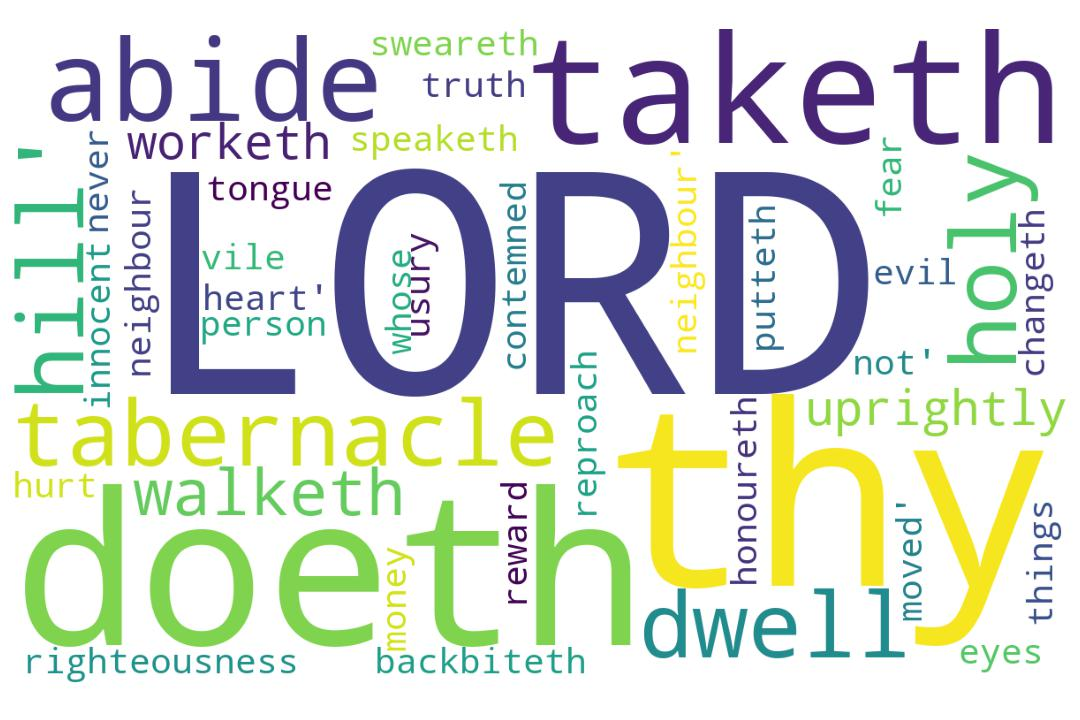
\includegraphics[width=\linewidth]{19OT-Psalms/Psalm15-WordCloud.jpg}
  \caption{Psalm 15 Word Cloud}
  \label{fig:Psalm 15 word Cloud}
\end{figure}



\marginpar{\scriptsize \centering \fcolorbox{bone}{lime}{\textbf{WHO DWELLS WITH GOD}}\\ (Psalm 15:1--5) \begin{compactenum}[I.][8]
    \item He who \textbf{Works Righteousness} \index[scripture]{Psalms!Psa 015:02} (Psa 15:2)
    \item He who \textbf{Meditates on Truth} \index[scripture]{Psalms!Psa 015:02} (Psa 15:2)
    \item He who \textbf{Does Not Backbite in Speech} -  (\index[scripture]{Psalms!Psa 015:03}Psa 15:3)
    \item He who \textbf{Treats his Neighbour Well} \index[scripture]{Psalms!Psa 015:03} \index[scripture]{Psalms!Psa 012:02} \index[scripture]{Psalms!Psa 101:05} (Psa 12:22, 15:3, and 101:5)
    \item He whose \textbf{Eyes Despise a Vile Man} \index[scripture]{Psalms!Psa 015:04} (Psa 15:4)
    \item He who \textbf{Does Not Put his Money Out to Usury} \index[scripture]{Psalms!Psa 015:05} (Psa 15:5) 
    \item He who \textbf{Does Not Betray the Brethren} \index[scripture]{Psalms!Psa 015:05} (Psa 15:5) 
\end{compactenum}}


\marginpar{\scriptsize \centering \fcolorbox{bone}{yellow}{\textbf{THE EVALUATION}}\\ (Psalm 15:1--5) \begin{compactenum}[I.][8]
    \item The \textbf{Everyday} Decisions 
    \item The \textbf{Eviction} Notice
    \item The \textbf{Event(s)} 
    \item The \textbf{Evidence} 
    \item The \textbf{Evil} Shunned and Avoided
    \item The \textbf{Evasion} from the Wicked
    \item The \textbf{Evaluation} 
\end{compactenum}}



\footnote{\textcolor[cmyk]{0.99998,1,0,0}{\hyperlink{TOC}{Return to end of Table of Contents.}}}\footnote{\href{https://www.audioverse.org/english/audiobibles/books/ENGKJV/O/Ps/1}{\textcolor[cmyk]{0.99998,1,0,0}{Psalms Audio}}}\textcolor[cmyk]{0.99998,1,0,0}{A Psalm of David.}\\
\\
\textcolor[cmyk]{0.99998,1,0,0}{LORD, who shall abide in thy tabernacle? who shall dwell in thy holy hill?}
[2] \textcolor[cmyk]{0.99998,1,0,0}{He that walketh uprightly, and \fcolorbox{bone}{lime}{worketh righteousness}, and \fcolorbox{bone}{lime}{speaketh the} \fcolorbox{bone}{lime}{truth in his} \fcolorbox{bone}{lime}{heart}.}
[3] \textcolor[cmyk]{0.99998,1,0,0}{\emph{He} \emph{that} \fcolorbox{bone}{lime}{backbiteth not} with his tongue, \fcolorbox{bone}{lime}{nor doeth} \fcolorbox{bone}{lime}{evil to his neighbour}, nor taketh up a reproach against his neighbour.}
[4] \textcolor[cmyk]{0.99998,1,0,0}{In whose eyes \fcolorbox{bone}{lime}{a vile person is} \fcolorbox{bone}{lime}{contemned}; but he honoureth them that fear the LORD. \emph{He} \emph{that} sweareth to \emph{his} \emph{own} hurt, and changeth not.}
[5] \textcolor[cmyk]{0.99998,1,0,0}{\emph{He} \emph{that} \fcolorbox{bone}{lime}{putteth not out his money} to usury, \fcolorbox{bone}{lime}{nor taketh reward} against the innocent. He that doeth these \emph{things} shall never be moved.}
\section{Psalm 15 Comments}

\subsection{Numeric Nuggets}
\textbf{5:} and \textbf{6:} Psalm 15 use the word ``his'' five times and adds the italic ``\emph{his}'' another time. In both cases, un-redeemed man (6 is the number of man) is destined for death (5 is the number of death).\\
\\
\textbf{13:} Verse 2 contains 13 unique words. The 13-letter word ``righteousness'' is found in the chapter. The word ``holy'' is the 13$^{th}$ word in the chapter.

\subsection{Psalm 15:1}
The fundamental problem the self-examining man must answer is verse 1. How do I get to God, or heaven? Who gets to go? Why? How? The answer, or answers, are found in scripture.  It is insufficient, arrogant, and vanity to come up with our own answers. We must seek out what God says about the matter. And just what if there are multiple, different, and even contradictory answers? Do you think it just might be wise to sort these out? Pretending there are no differences must just be a unwise approach, especially since getting this question wrong will land some body in Hell. Perhaps we ought to find out what God requires, and then meet that requirement. Evidently, from Psalm 15, someone, at sometime, has a different set of rules than I do, saved by grace through faith.\\
\\
Let's start out by pointing Ephesians 2:8-9, for the New Testament Christian. I am headed to heaven simply by belief. I am very likely guilt of things listed in Psalm 15, but I have a substitute, a replacement, who is not. I have admitted my guilt, acknowledged by deserved punishment, and accepted the payment of Jesus Christ on my behalf. Afterwards, I act as the new creature I have been made. The works come afterward. Here, in Psalm 15, the words come before. \footnote{\textbf{Ephesians 2:8-9} - For by grace are ye saved through faith; and that not of yourselves: it is the gift of God: [9] Not of works, lest any man should boast.}\\
\\
This psalm, though, presents a list of things one must do to get to the ``tabernacle'' and to the ``holy hill.'' The list:
\begin{compactenum}
    \item Walk uprightly [1],
    \item Work righteousness [1],
    \item Speaks the truth in his heart [1],
    \item Does not backbite [2],
    \item Does not do evil to his neighbour [2],
    \item Does not take up a reproach against his neighbour [2],
    \item Recognizes and condemns evil [3],
    \item Honours them that fear the Lord [3],
    \item Swears to his own hurt [3],
    \item Doesn't change [3] (endures),
    \item Does not loan with interest [4], and
    \item Does not take bribes [4].\\
\end{compactenum}
\noindent The same question is asked in Psalm 24:3.\footnote{\textbf{Psalm 24:3} - Who shall ascend into the hill of the LORD? or who shall stand in his holy place?} Psalm 24 is the parallel passage. In it, as here, the Lord is reigning on earth, and has a tabernacle, on a holy hill, as described in Psalm 2:6.\footnote{\textbf{Psalm 2:6} - Yet have I set my king upon my holy hill of Zion}. This is after God has spoken to the heathen in wrath (Psalm 2:5) and vexed them. The Lord is not currently reigning on earth, not in Jerusalem, or on any of the seven hills of Rome. The context is beautifully described in Isaiah 2:2-5 and 33:20-24.\footnote{\textbf{Isaiah 2:2-5} - And it shall come to pass in the last days, that the mountain of the LORD’S house shall be established in the top of the mountains, and shall be exalted above the hills; and all nations shall flow unto it. [3] And many people shall go and say, Come ye, and let us go up to the mountain of the LORD, to the house of the God of Jacob; and he will teach us of his ways, and we will walk in his paths: for out of Zion shall go forth the law, and the word of the LORD from Jerusalem. [4] And he shall judge among the nations, and shall rebuke many people: and they shall beat their swords into plowshares, and their spears into pruninghooks: nation shall not lift up sword against nation, neither shall they learn war any more. [5] O house of Jacob, come ye, and let us walk in the light of the LORD.}\footnote{\textbf{Isaiah 33:20-24} - Look upon Zion, the city of our solemnities: thine eyes shall see Jerusalem a quiet habitation, a tabernacle that shall not be taken down; not one of the stakes thereof shall ever be removed, neither shall any of the cords thereof be broken. [21] But there the glorious LORD will be unto us a place of broad rivers and streams; wherein shall go no galley with oars, neither shall gallant ship pass thereby. [22] For the LORD is our judge, the LORD is our lawgiver, the LORD is our king; he will save us. [23] Thy tacklings are loosed; they could not well strengthen their mast, they could not spread the sail: then is the prey of a great spoil divided; the lame take the prey. [24] And the inhabitant shall not say, I am sick: the people that dwell therein shall be forgiven their iniquity.}This temple is described in Ezekiel 4-46. It is a Jewish context. The Lord is on a throne in Jerusalem in the midst of a Jewish Millennial kingdom, a kingdom of righteousness. Remember John 4:22? Salvation is of the Jew.\footnote{\textbf{John 4:22} - \textcolor[cmyk]{0,1,0,0}{Ye worship ye know not what: we know what we worship: for salvation is of the Jews.}}\\
\\
Psalm 15 is describing the works necessary, the conditions, necessary to enter this rebuilt temple. Consider the warning passages, pointed out by Ruckman: Psalm 18:20\footnote{\textbf{Psalm 18:20} - The LORD rewarded me according to my righteousness; according to the cleanness of my hands hath he recompensed me.}, Matthew 24:13\footnote{\textbf{Matthew 24:13} - \textcolor[cmyk]{0,1,0,0}{But he that shall endure unto the end, the same shall be saved.}}, Hebrews 3:14\footnote{\textbf{Hebrews 3:14} - For we are made partakers of Christ, if we hold the beginning of our confidence stedfast unto the end;}, 6:6\footnote{\textbf{Hebrews 6:6} -  If they shall fall away, to renew them again unto repentance; seeing they crucify to themselves the Son of God afresh, and put him to an open shame.}, 10:23\footnote{\textbf{Hebrews 10:23} -  If they shall fall away, to renew them again unto repentance; seeing they crucify to themselves the Son of God afresh, and put him to an open shame.}, Revelation 12:11\footnote{\textbf{Revelation 12:11} - And they overcame him by the blood of the Lamb, and by the word of their testimony; and they loved not their lives unto the death.}, 14:4 \footnote{\textbf{Revelation 14:4} - These are they which were not defiled with women; for they are virgins. These are they which follow the Lamb whithersoever he goeth. These were redeemed from among men, being the firstfruits unto God and to the Lamb.}. \cite{Ruckman1992PsalmsV1} \\
\\
Kidner\cite{kidner2014psalmsV1} and Phillips have the psalm describing a ``guest in the Lord's house,'' and focusing on expected and proper behavior once inside. This is different, of course, than actual requirements to get in! Phillips does, though, describe the probable connection between Psalm 15 and the Sermon on the Mount.  \cite[121]{Phillips2001ExploringPsalms1}\\
\\
\noindent Boice comments on Psalm 15 by pointing out that David's answers were \emph{representative} - his list, here, was not all-inclusive. Other lists are provided in Psalm 24:3-4\footnote{\textbf{Psalm 24:3-4} - Who shall ascend into the hill of the LORD? or who shall stand in his holy place? [4] He that hath clean hands, and a pure heart; who hath not lifted up his soul unto vanity, nor sworn deceitfully.} and Isaiah 33:14-17.\footnote{\textbf{Isaiah 33:14-17} - The sinners in Zion are afraid; fearfulness hath surprised the hypocrites. Who among us shall dwell with the devouring fire? who among us shall dwell with everlasting burnings? 15 [He] that walketh righteously, and speaketh uprightly; he that despiseth the gain of oppressions, that shaketh his hands from holding of bribes, that stoppeth his ears from hearing of blood, and shutteth his eyes from seeing evil; [16] He shall dwell on high: his place of defence shall be the munitions of rocks: bread shall be given him; his waters shall be sure. [17] Thine eyes shall see the king in his beauty: they shall behold the land that is very far off.}\cite{boice2005psalmsV1} He continues with comments on the six couplets he sees in the psalm, which follow the parallelism in the Hebrew text. These couplets provide an outline for the psalm, ``The Person God Approves'':\\

\begin{compactenum}[I.]
    \item His character 
    \item His speech
    \item His conduct
    \item His values
    \item His integrity
    \item His use of money\\

\end{compactenum}

\noindent Psalm 15 is captured in the hymn by Isaac Watts:
\begin{quote}
Who shall ascend thy heav'nly place,\\
Great God, and dwell before thy face?\\
The man that minds religion now,\\
And humbly walks with God below;\\
\\
Whose hands are pure, whose heart is clean,\\
Whose lips still speak the thing they mean;\\
No slanders dwell upon his tongue;\\
He hates to do his neighbor wrong.\\
\\
- Scarce will he trust an ill report,\\
Nor vents it to his neighbor's hurt:\\
Sinners of state he can despise,\\
But saints are honored in his eyes. -\\
\\
- Firm to his word he ever stood,\\
And always makes his promise good;\\
Nor dares to change the thing he swears,\\
Whatever pain or loss he bears.- \\
\\
- He never deals in bribing gold,\\
And mourns that justice should be sold;\\
While others gripe and grind the poor,\\
Sweet charity attends his door. -\\
\\
He loves his enemies, and prays\\
For those that curse him to his face\\
And doth to all men still the same\\
That he would hope or wish from them.\\
\\
Yet, when his holiest works are done,\\
His soul depends on grace alone:\\
This is the man thy face shall see,\\
And dwell for ever, Lord, with thee.   \\
\end{quote}
%\index[NWIV]{14!Psalms!Psa 15:1}\index[AWIP]{LORD!Psalms!Psa 15:1}\index[AWIP]{who!Psalms!Psa 15:1}\index[AWIP]{who!Psalms!Psa 15:1 (2)}\index[AWIP]{shall!Psalms!Psa 15:1}\index[AWIP]{shall!Psalms!Psa 15:1 (2)}\index[AWIP]{abide!Psalms!Psa 15:1}\index[AWIP]{in!Psalms!Psa 15:1}\index[AWIP]{in!Psalms!Psa 15:1 (2)}\index[AWIP]{thy!Psalms!Psa 15:1}\index[AWIP]{thy!Psalms!Psa 15:1 (2)}\index[AWIP]{tabernacle?!Psalms!Psa 15:1}\index[AWIP]{dwell!Psalms!Psa 15:1}\index[AWIP]{holy!Psalms!Psa 15:1}\index[AWIP]{hill?!Psalms!Psa 15:1}

\index[NWIV]{14!Psalms!Psa 15:2}\index[AWIP]{He!Psalms!Psa 15:2}\index[AWIP]{that!Psalms!Psa 15:2}\index[AWIP]{walketh!Psalms!Psa 15:2}\index[AWIP]{uprightly!Psalms!Psa 15:2}\index[AWIP]{and!Psalms!Psa 15:2}\index[AWIP]{and!Psalms!Psa 15:2 (2)}\index[AWIP]{worketh!Psalms!Psa 15:2}\index[AWIP]{righteousness!Psalms!Psa 15:2}\index[AWIP]{speaketh!Psalms!Psa 15:2}\index[AWIP]{the!Psalms!Psa 15:2}\index[AWIP]{truth!Psalms!Psa 15:2}\index[AWIP]{in!Psalms!Psa 15:2}\index[AWIP]{his!Psalms!Psa 15:2}\index[AWIP]{heart!Psalms!Psa 15:2}

\index[NWIV]{21!Psalms!Psa 15:3}\index[AWIP]{\emph{He}!Psalms!Psa 15:3}\index[AWIP]{\emph{that}!Psalms!Psa 15:3}\index[AWIP]{backbiteth!Psalms!Psa 15:3}\index[AWIP]{not!Psalms!Psa 15:3}\index[AWIP]{with!Psalms!Psa 15:3}\index[AWIP]{his!Psalms!Psa 15:3}\index[AWIP]{his!Psalms!Psa 15:3 (2)}\index[AWIP]{his!Psalms!Psa 15:3 (3)}\index[AWIP]{tongue!Psalms!Psa 15:3}\index[AWIP]{nor!Psalms!Psa 15:3}\index[AWIP]{nor!Psalms!Psa 15:3 (2)}\index[AWIP]{doeth!Psalms!Psa 15:3}\index[AWIP]{evil!Psalms!Psa 15:3}\index[AWIP]{to!Psalms!Psa 15:3}\index[AWIP]{neighbour!Psalms!Psa 15:3}\index[AWIP]{neighbour!Psalms!Psa 15:3 (2)}\index[AWIP]{taketh!Psalms!Psa 15:3}\index[AWIP]{up!Psalms!Psa 15:3}\index[AWIP]{a!Psalms!Psa 15:3}\index[AWIP]{reproach!Psalms!Psa 15:3}\index[AWIP]{against!Psalms!Psa 15:3}\index[AWIP]{\emph{He}!Psalms!Psa 15:3}\index[AWIP]{\emph{that}!Psalms!Psa 15:3}

\index[NWIV]{26!Psalms!Psa 15:4}\index[AWIP]{In!Psalms!Psa 15:4}\index[AWIP]{whose!Psalms!Psa 15:4}\index[AWIP]{eyes!Psalms!Psa 15:4}\index[AWIP]{a!Psalms!Psa 15:4}\index[AWIP]{vile!Psalms!Psa 15:4}\index[AWIP]{person!Psalms!Psa 15:4}\index[AWIP]{is!Psalms!Psa 15:4}\index[AWIP]{contemned!Psalms!Psa 15:4}\index[AWIP]{but!Psalms!Psa 15:4}\index[AWIP]{he!Psalms!Psa 15:4}\index[AWIP]{honoureth!Psalms!Psa 15:4}\index[AWIP]{them!Psalms!Psa 15:4}\index[AWIP]{that!Psalms!Psa 15:4}\index[AWIP]{fear!Psalms!Psa 15:4}\index[AWIP]{the!Psalms!Psa 15:4}\index[AWIP]{LORD!Psalms!Psa 15:4}\index[AWIP]{\emph{He}!Psalms!Psa 15:4}\index[AWIP]{\emph{that}!Psalms!Psa 15:4}\index[AWIP]{sweareth!Psalms!Psa 15:4}\index[AWIP]{to!Psalms!Psa 15:4}\index[AWIP]{\emph{his}!Psalms!Psa 15:4}\index[AWIP]{\emph{own}!Psalms!Psa 15:4}\index[AWIP]{hurt!Psalms!Psa 15:4}\index[AWIP]{and!Psalms!Psa 15:4}\index[AWIP]{changeth!Psalms!Psa 15:4}\index[AWIP]{not!Psalms!Psa 15:4}\index[AWIP]{\emph{He}!Psalms!Psa 15:4}\index[AWIP]{\emph{that}!Psalms!Psa 15:4}\index[AWIP]{\emph{his}!Psalms!Psa 15:4}\index[AWIP]{\emph{own}!Psalms!Psa 15:4}

\index[NWIV]{24!Psalms!Psa 15:5}\index[AWIP]{\emph{He}!Psalms!Psa 15:5}\index[AWIP]{\emph{that}!Psalms!Psa 15:5}\index[AWIP]{putteth!Psalms!Psa 15:5}\index[AWIP]{not!Psalms!Psa 15:5}\index[AWIP]{out!Psalms!Psa 15:5}\index[AWIP]{his!Psalms!Psa 15:5}\index[AWIP]{money!Psalms!Psa 15:5}\index[AWIP]{to!Psalms!Psa 15:5}\index[AWIP]{usury!Psalms!Psa 15:5}\index[AWIP]{nor!Psalms!Psa 15:5}\index[AWIP]{taketh!Psalms!Psa 15:5}\index[AWIP]{reward!Psalms!Psa 15:5}\index[AWIP]{against!Psalms!Psa 15:5}\index[AWIP]{the!Psalms!Psa 15:5}\index[AWIP]{innocent!Psalms!Psa 15:5}\index[AWIP]{He!Psalms!Psa 15:5}\index[AWIP]{that!Psalms!Psa 15:5}\index[AWIP]{doeth!Psalms!Psa 15:5}\index[AWIP]{these!Psalms!Psa 15:5}\index[AWIP]{\emph{things}!Psalms!Psa 15:5}\index[AWIP]{shall!Psalms!Psa 15:5}\index[AWIP]{never!Psalms!Psa 15:5}\index[AWIP]{be!Psalms!Psa 15:5}\index[AWIP]{moved!Psalms!Psa 15:5}\index[AWIP]{\emph{He}!Psalms!Psa 15:5}\index[AWIP]{\emph{that}!Psalms!Psa 15:5}\index[AWIP]{\emph{things}!Psalms!Psa 15:5}


\section{Psalm 15 Outlines}

\subsection{My Outlines}

\subsubsection{Who Gets to Dwell with God?}
\textbf{Introduction:} Psalm 15 gives us a list of who gets to dwell with God, who gets to dwell in the holy hill of Zion? Note that in the Millennium, there will be a literal holy hill in Jerusalem!:
\index[speaker]{Keith Anthony!Psalm 015 (Who Gets to Dwell with God?)}
\index[series]{Psalms (Keith Anthony)!Psalm 015 (Who Gets to Dwell with God?)}
\index[date]{2015/11/15!Psalm 015 (Who Gets to Dwell with God?) (Keith Anthony)}
\begin{compactenum}
    \item He who \textbf{Works Righteousness} \index[scripture]{Psalms!Psa 015:02} (Psa 15:2)
    \item He who \textbf{Meditates on Truth} \index[scripture]{Psalms!Psa 015:02} (Psa 15:2)
    \item He who \textbf{Does Not Backbite in Speech} -  (\index[scripture]{Psalms!Psa 015:03}Psa 15:3)
    \item He who \textbf{Treats his Neighbour Well} \index[scripture]{Psalms!Psa 015:03} \index[scripture]{Psalms!Psa 012:02} \index[scripture]{Psalms!Psa 101:05} (Psa 12:22, 15:3, and 101:5)
    \item He whose \textbf{Eyes Despise a Vile Man} \index[scripture]{Psalms!Psa 015:04} (Psa 15:4)
    \item He who \textbf{Does Not Put his Money Out to Usury} \index[scripture]{Psalms!Psa 015:05} (Psa 15:5) 
    \item He who \textbf{Does Not Betray the Brethren} \index[scripture]{Psalms!Psa 015:05} (Psa 15:5) 
\end{compactenum}


\subsubsection{The Evaluation}
%\textbf{Introduction:} Psalm 15 gives us a list of who gets to dwell with God, who gets to dwell in the holy hill of Zion? Note that in the Millennium, there will be a literal holy hill in Jerusalem!:
\index[speaker]{Keith Anthony!Psalm 015 (The Evaluation)}
\index[series]{Psalms (Keith Anthony)!Psalm 015 (The Evaluation?)}
\index[date]{2022/01/15!Psalm 015 (The Evaluation) (Keith Anthony)}
\begin{compactenum} 
    \item The \textbf{Everyday} Decisions 
    \item The \textbf{Eviction} Notice
    \item The \textbf{Event(s)} 
    \item The \textbf{Evidence} 
    \item The \textbf{Evil} Shunned and Avoided
    \item The \textbf{Evasion} from the Wickws
    \item The \textbf{Evaluation} 
\end{compactenum}


\subsection{Outlines from Others}



%\section{Psalm 15 Statistics}

%%%%%%%%%%%%%%%%%%%%%%%%%%%
%%%%%Word Statistics
%%%%%%%%%%%%%%%%%%%%%%%%%%%


\normalsize



\subsection{Chapter Word Statistics}


%%%%%%%%%%
%%%%%%%%%%
 
\begin{center}
\begin{longtable}{l|c|c|c|c}
\caption[Stats for Psalm 15]{Stats for Psalm 15} \label{table:Stats for Psalm 15} \\ 
\hline \multicolumn{1}{|c|}{\textbf{Verse(s)}} & \multicolumn{1}{|c|}{\textbf{Count}} & \multicolumn{1}{|c|}{\textbf{Unique}} & \multicolumn{1}{|c|}{\textbf{Italics}} & \multicolumn{1}{|c|}{\textbf{Uniq Italic}}  \\ \hline 
\endfirsthead
 
\multicolumn{5}{c}
{{\bfseries \tablename\ \thetable{} -- continued from previous page}} \\  
\hline \multicolumn{1}{|c|}{\textbf{Verse(s)}} & \multicolumn{1}{|c|}{\textbf{Count}} & \multicolumn{1}{|c|}{\textbf{Unique}} & \multicolumn{1}{|c|}{\textbf{Italics}} & \multicolumn{1}{|c|}{\textbf{Uniq Italic}}  \\ \hline 
\endhead
 
\hline \multicolumn{5}{|r|}{{Continued if needed}} \\ \hline
\endfoot 
1 & 14 & 10 & 0 & 0\\ \hline
2 & 14 & 13 & 0 & 0\\ \hline
3 & 21 & 17 & 2 & 2\\ \hline
4 & 26 & 26 & 4 & 4\\ \hline
5 & 24 & 24 & 3 & 3\\ \hline
\hline \hline
Total & 99 & 66 & 9 & 5



\end{longtable}
\end{center}

%%%%%%%%%%
%%%%%%%%%%
 
\subsection{Words by Frequency}

\begin{center}
\begin{longtable}{l|r}
\caption[Word Frequencies in Psalm 15]{Word Frequencies in Psalm 15} \label{table:WordsIn-Psalm-15} \\ 
\hline \multicolumn{1}{|c|}{\textbf{Word}} & \multicolumn{1}{c|}{\textbf{Frequency}} \\ \hline 
\endfirsthead
 
\multicolumn{2}{c}
{{\bfseries \tablename\ \thetable{} -- continued from previous page}} \\ 
\hline \multicolumn{1}{|c|}{\textbf{Word}} & \multicolumn{1}{c|}{\textbf{Frequency}} \\ \hline 
\endhead
 
\hline \multicolumn{2}{|r|}{{Continued if needed}} \\ \hline
\endfoot
 
\hline \hline
\endlastfoot
his & 5 \\ \hline
shall & 3 \\ \hline
in & 3 \\ \hline
that & 3 \\ \hline
and & 3 \\ \hline
the & 3 \\ \hline
\emph{He} & 3 \\ \hline
\emph{that} & 3 \\ \hline
not & 3 \\ \hline
nor & 3 \\ \hline
to & 3 \\ \hline
LORD & 2 \\ \hline
who & 2 \\ \hline
thy & 2 \\ \hline
He & 2 \\ \hline
doeth & 2 \\ \hline
neighbour & 2 \\ \hline
taketh & 2 \\ \hline
a & 2 \\ \hline
against & 2 \\ \hline
abide & 1 \\ \hline
tabernacle & 1 \\ \hline
dwell & 1 \\ \hline
holy & 1 \\ \hline
hill & 1 \\ \hline
walketh & 1 \\ \hline
uprightly & 1 \\ \hline
worketh & 1 \\ \hline
righteousness & 1 \\ \hline
speaketh & 1 \\ \hline
truth & 1 \\ \hline
heart & 1 \\ \hline
backbiteth & 1 \\ \hline
with & 1 \\ \hline
tongue & 1 \\ \hline
evil & 1 \\ \hline
up & 1 \\ \hline
reproach & 1 \\ \hline
In & 1 \\ \hline
whose & 1 \\ \hline
eyes & 1 \\ \hline
vile & 1 \\ \hline
person & 1 \\ \hline
is & 1 \\ \hline
contemned & 1 \\ \hline
but & 1 \\ \hline
he & 1 \\ \hline
honoureth & 1 \\ \hline
them & 1 \\ \hline
fear & 1 \\ \hline
sweareth & 1 \\ \hline
\emph{his} & 1 \\ \hline
\emph{own} & 1 \\ \hline
hurt & 1 \\ \hline
changeth & 1 \\ \hline
putteth & 1 \\ \hline
out & 1 \\ \hline
money & 1 \\ \hline
usury & 1 \\ \hline
reward & 1 \\ \hline
innocent & 1 \\ \hline
these & 1 \\ \hline
\emph{things} & 1 \\ \hline
never & 1 \\ \hline
be & 1 \\ \hline
moved & 1 \\ \hline
\end{longtable}
\end{center}



\normalsize



\subsection{Words Alphabetically}

\begin{center}
\begin{longtable}{l|r}
\caption[Word Alphabetically in Psalm 15]{Word Alphabetically in Psalm 15} \label{table:WordsIn-Psalm-15} \\ 
\hline \multicolumn{1}{|c|}{\textbf{Word}} & \multicolumn{1}{c|}{\textbf{Frequency}} \\ \hline 
\endfirsthead
 
\multicolumn{2}{c}
{{\bfseries \tablename\ \thetable{} -- continued from previous page}} \\ 
\hline \multicolumn{1}{|c|}{\textbf{Word}} & \multicolumn{1}{c|}{\textbf{Frequency}} \\ \hline 
\endhead
 
\hline \multicolumn{2}{|r|}{{Continued if needed}} \\ \hline
\endfoot
 
\hline \hline
\endlastfoot
He & 2 \\ \hline
In & 1 \\ \hline
LORD & 2 \\ \hline
\emph{He} & 3 \\ \hline
\emph{his} & 1 \\ \hline
\emph{own} & 1 \\ \hline
\emph{that} & 3 \\ \hline
\emph{things} & 1 \\ \hline
a & 2 \\ \hline
abide & 1 \\ \hline
against & 2 \\ \hline
and & 3 \\ \hline
backbiteth & 1 \\ \hline
be & 1 \\ \hline
but & 1 \\ \hline
changeth & 1 \\ \hline
contemned & 1 \\ \hline
doeth & 2 \\ \hline
dwell & 1 \\ \hline
evil & 1 \\ \hline
eyes & 1 \\ \hline
fear & 1 \\ \hline
he & 1 \\ \hline
heart & 1 \\ \hline
hill & 1 \\ \hline
his & 5 \\ \hline
holy & 1 \\ \hline
honoureth & 1 \\ \hline
hurt & 1 \\ \hline
in & 3 \\ \hline
innocent & 1 \\ \hline
is & 1 \\ \hline
money & 1 \\ \hline
moved & 1 \\ \hline
neighbour & 2 \\ \hline
never & 1 \\ \hline
nor & 3 \\ \hline
not & 3 \\ \hline
out & 1 \\ \hline
person & 1 \\ \hline
putteth & 1 \\ \hline
reproach & 1 \\ \hline
reward & 1 \\ \hline
righteousness & 1 \\ \hline
shall & 3 \\ \hline
speaketh & 1 \\ \hline
sweareth & 1 \\ \hline
tabernacle & 1 \\ \hline
taketh & 2 \\ \hline
that & 3 \\ \hline
the & 3 \\ \hline
them & 1 \\ \hline
these & 1 \\ \hline
thy & 2 \\ \hline
to & 3 \\ \hline
tongue & 1 \\ \hline
truth & 1 \\ \hline
up & 1 \\ \hline
uprightly & 1 \\ \hline
usury & 1 \\ \hline
vile & 1 \\ \hline
walketh & 1 \\ \hline
who & 2 \\ \hline
whose & 1 \\ \hline
with & 1 \\ \hline
worketh & 1 \\ \hline
\end{longtable}
\end{center}



\normalsize



\subsection{Word Lengths in Chapter}
\normalsize
\begin{longtable}{l|p{3.75in}}
\caption[Words by Length in Psalm 15]{Words by Length in Psalm 15} \label{table:WordsIn-Psalm-15} \\ 
\hline \multicolumn{1}{|c|}{\textbf{Length}} & \multicolumn{1}{c|}{\textbf{Words}} \\ \hline 
\endfirsthead
 
\multicolumn{2}{c}
{{\bfseries \tablename\ \thetable{} -- continued from previous page}} \\ 
\hline \multicolumn{1}{|c|}{\textbf{Length}} & \multicolumn{1}{c|}{\textbf{Words}} \\ \hline 
\endhead
 
\hline \multicolumn{2}{|r|}{{Continued if needed}} \\ \hline
\endfoot
 
\hline \hline
\endlastfoot
1 & a \\ \hline
2 & in, He, \emph{He}, to, up, In, is, he, be \\ \hline
3 & who, thy, and, the, his, not, nor, but, \emph{his}, \emph{own}, out \\ \hline
4 & LORD, holy, hill, that, \emph{that}, with, evil, eyes, vile, them, fear, hurt \\ \hline
5 & shall, abide, dwell, truth, heart, doeth, whose, money, usury, these, never, moved \\ \hline
6 & tongue, taketh, person, reward, \emph{things} \\ \hline
7 & walketh, worketh, against, putteth \\ \hline
8 & speaketh, reproach, sweareth, changeth, innocent \\ \hline
9 & uprightly, neighbour, contemned, honoureth \\ \hline
10 & tabernacle, backbiteth \\ \hline
13 & righteousness \\ \hline
\end{longtable}






%%%%%%%%%%
%%%%%%%%%%
\subsection{Psalm 15 Repeated Phrases}


%%%%%%%%%%
%%%%%%%%%%
\normalsize
 
\begin{center}
\begin{longtable}{|p{3.0in}|p{0.5in}|}
\caption[Psalm 15 Repeated Phrases]{Psalm 15 Repeated Phrases}\label{table:Repeated Phrases Psalm 5} \\
\hline \multicolumn{1}{|c|}{\textbf{Phrase}} & \multicolumn{1}{c|}{\textbf{Frequency}} \\ \hline 
\endfirsthead
 
\multicolumn{2}{c}
{{\bfseries \tablename\ \thetable{} -- continued from previous page}} \\  
\hline \multicolumn{1}{|c|}{\textbf{Phrase}} & \multicolumn{1}{c|}{\textbf{Frequency}} \\ \hline 
\endhead
 
\hline \multicolumn{2}{c}{{ }} \\ \hline
\endfoot 
\emph{He} \emph{that} & 3\\ \hline 
\end{longtable}
\end{center}



%%%%%%%%%%
%%%%%%%%%%




\chapter{Psalm 16}

\begin{figure}
  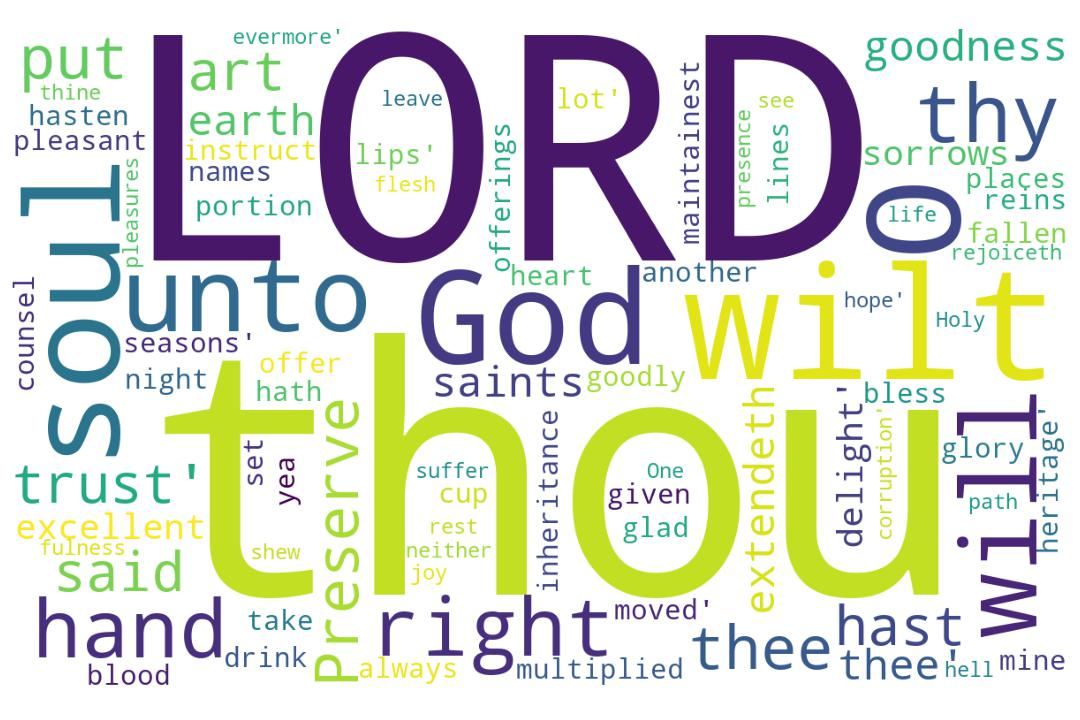
\includegraphics[width=\linewidth]{19OT-Psalms/Psalm16-WordCloud.jpg}
  \caption{Psalm 16 Word Cloud}
  \label{fig:Psalm 16 word Cloud}
\end{figure}



\marginpar{\scriptsize \centering \fcolorbox{bone}{lime}{\textbf{CONTRASTS}}\\ (Psalm 16:1--11) \begin{compactenum}[I.][8]
	\item Thirteen \textbf{Possession} \index[scripture]{Psalms!Psa 016:01}(Psa 16:1)
	\begin{compactenum}[A.]
	    \item My \textbf{trust} \index[scripture]{Psalms!Psa 016:01}(Psa 16:1)
	    \item My \textbf{soul} \index[scripture]{Psalms!Psa 016:02}(Psa 16:2)
	    \item My \textbf{Lord} \index[scripture]{Psalms!Psa 016:02}(Psa 16:2)
	    \item My \textbf{goodness} \index[scripture]{Psalms!Psa 016:02}(Psa 16:2)
	    \item My \textbf{delight} \index[scripture]{Psalms!Psa 016:03}(Psa 16:3)
	    \item My \textbf{lips} \index[scripture]{Psalms!Psa 016:04}(Psa 16:4)
	    \item My \textbf{cup} \index[scripture]{Psalms!Psa 016:05}(Psa 16:5)
	    \item My \textbf{lot} \index[scripture]{Psalms!Psa 016:05}(Psa 16:5)
	    \item My \textbf{right hand} \index[scripture]{Psalms!Psa 016:08}(Psa 16:8)
	    \item My \textbf{heart} \index[scripture]{Psalms!Psa 016:09}(Psa 16:9)
	    \item My \textbf{glory} \index[scripture]{Psalms!Psa 016:09}(Psa 16:9)
	    \item My \textbf{flesh} \index[scripture]{Psalms!Psa 016:09}(Psa 16:9)
	    \item My \textbf{soul} \index[scripture]{Psalms!Psa 016:10}(Psa 16:10)
	\end{compactenum}
	\item One \textbf{Provision} (thine Holy One) \index[scripture]{Psalms!Psa 016:10}(Psa 16:10)
	\item One \textbf{Promise} (mine inheritance) \index[scripture]{Psalms!Psa 016:05}(Psa 16:5)
\end{compactenum}}

\footnote{\textcolor[cmyk]{0.99998,1,0,0}{\hyperlink{TOC}{Return to end of Table of Contents.}}}\footnote{\href{https://www.audioverse.org/english/audiobibles/books/ENGKJV/O/Ps/1}{\textcolor[cmyk]{0.99998,1,0,0}{Psalms Audio}}}\textcolor[cmyk]{0.99998,1,0,0}{Michtam of David.}\\
\\
\textcolor[cmyk]{0.99998,1,0,0}{Preserve me, O God: for in thee do I put \fcolorbox{bone}{lime}{my trust}.}\footnote{\textbf{Psalm 17:5,8} - Hold up my goings in thy paths, that my footsteps slip not. [8] Keep me as the apple of the eye, hide me under the shadow of thy wings,}\footnote{\textbf{Psalm 31:23} - O love the LORD, all ye his saints: for the LORD preserveth the faithful, and plentifully rewardeth the proud doer.}\footnote{\textbf{Psalm 37:28} - For the LORD loveth judgment, and forsaketh not his saints; they are preserved for ever: but the seed of the wicked shall be cut off.}\footnote{\textbf{Psalm 56:1} - Be merciful unto me, O God: for man would swallow me up; he fighting daily oppresseth me.}\footnote{\textbf{Psalm 60:1} - O God, thou hast cast us off, thou hast scattered us, thou hast been displeased; O turn thyself to us again.}\footnote{\textbf{Psalm 97:10} - Ye that love the LORD, hate evil: he preserveth the souls of his saints; he delivereth them out of the hand of the wicked.}\footnote{\textbf{Psalm 116:6} - The LORD preserveth the simple: I was brought low, and he helped me.}\footnote{\textbf{Proverb 2:8} - He keepeth the paths of judgment, and preserveth the way of his saints.}\footnote{\textbf{Isaiah 26:3-4} - Thou wilt keep him in perfect peace, whose mind is stayed on thee: because he trusteth in thee. [4] Trust ye in the LORD for ever: for in the LORD JEHOVAH is everlasting strength:}\footnote{\textbf{2 Corinthians 1:9} - But we had the sentence of death in ourselves, that we should not trust in ourselves, but in God which raiseth the dead:}\footnote{\textbf{2 Timothy 1:12} - For the which cause I also suffer these things: nevertheless I am not ashamed: for I know whom I have believed, and am persuaded that he is able to keep that which I have committed unto him against that day.}
[2] \textcolor[cmyk]{0.99998,1,0,0}{\emph{O} \fcolorbox{bone}{lime}{\emph{my} \emph{soul}}, thou hast said unto the LORD, Thou \emph{art} \fcolorbox{bone}{lime}{my Lord}: \fcolorbox{bone}{lime}{my goodness} \emph{extendeth} not to thee;}\footnote{\textbf{Job 22:2-3} - Can a man be profitable unto God, as he that is wise may be profitable unto himself? [3] Is it any pleasure to the Almighty, that thou art righteous? or is it gain to him, that thou makest thy ways perfect?}\footnote{\textbf{Job 35:7-8} - If thou be righteous, what givest thou him? or what receiveth he of thine hand? [8] Thy wickedness may hurt a man as thou art; and thy righteousness may profit the son of man.}\footnote{\textbf{John 20:28} - And Thomas answered and said unto him, My Lord and my God.}
[3] \textcolor[cmyk]{0.99998,1,0,0}{\emph{But} to the saints that \emph{are} in the earth, and \emph{to} the excellent, in whom \emph{is} all \fcolorbox{bone}{lime}{my delight}.}\footnote{\textbf{Psalm 30:4} - Sing unto the LORD, O ye saints of his, and give thanks at the remembrance of his holiness.}
[4] \textcolor[cmyk]{0.99998,1,0,0}{Their sorrows shall be multiplied \emph{that} hasten \emph{after} another \emph{god}: their drink offerings of blood will I not offer, nor take up their names into \fcolorbox{bone}{lime}{my lips}.}\footnote{\textbf{Psalm 32:10} - Many sorrows shall be to the wicked: but he that trusteth in the LORD, mercy shall compass him about.}\footnote{\textbf{Psalm 97:7} - Confounded be all they that serve graven images, that boast themselves of idols: worship him, all ye gods.}\footnote{\textbf{Jonah 2:8} - They that observe lying vanities forsake their own mercy.}\footnote{\textbf{Genesis 35:14} - And Jacob set up a pillar in the place where he talked with him, even a pillar of stone: and he poured a drink offering thereon, and he poured oil thereon.}
[5] \textcolor[cmyk]{0.99998,1,0,0}{The LORD \emph{is} the portion of mine inheritance and of \fcolorbox{bone}{lime}{my cup}: thou maintainest \fcolorbox{bone}{lime}{my lot}.}\footnote{\textbf{Psalm 73:26} - My flesh and my heart faileth: but God is the strength of my heart, and my portion for ever.}\footnote{\textbf{Psalm 119:57} - Thou art my portion, O LORD: I have said that I would keep thy words.}\footnote{\textbf{Psalm 142:5} - I cried unto thee, O LORD: I said, Thou art my refuge and my portion in the land of the living.}\footnote{\textbf{Deuteronomy 32:9} - For the LORD'S portion is his people; Jacob is the lot of his inheritance.}\footnote{\textbf{Jeremiah 10:16} - The portion of Jacob is not like them: for he is the former of all things; and Israel is the rod of his inheritance: The LORD of hosts is his name.}\footnote{\textbf{Lamentations 3:24} - The LORD is my portion, saith my soul; therefore will I hope in him.}
[6] \textcolor[cmyk]{0.99998,1,0,0}{The lines are fallen unto me in pleasant \emph{places}; yea, I have a goodly heritage.}
[7] \textcolor[cmyk]{0.99998,1,0,0}{I will bless the LORD, who hath given me counsel: my reins also instruct me in the night seasons.}
[8] \textcolor[cmyk]{0.99998,1,0,0}{I have set the LORD always before me: because \emph{he} \emph{is} at \fcolorbox{bone}{lime}{my right hand}, I shall not be moved.}
[9] \textcolor[cmyk]{0.99998,1,0,0}{Therefore \fcolorbox{bone}{lime}{my heart} is glad, and \fcolorbox{bone}{lime}{my glory} rejoiceth: \fcolorbox{bone}{lime}{my flesh} also shall rest in hope.}
[10] \textcolor[cmyk]{0.99998,1,0,0}{For thou wilt not leave \fcolorbox{bone}{lime}{my soul} in hell; neither wilt thou suffer thine Holy One to see corruption.}\footnote{\textbf{Acts 2:27, 31} - Because thou wilt not leave my soul in hell, neither wilt thou suffer thine Holy One to see corruption. [31] He seeing this before spake of the resurrection of Christ, that his soul was not left in hell, neither his flesh did see corruption.}\footnote{\textbf{Acts 13:34-37} - And as concerning that he raised him up from the dead, now no more to return to corruption, he said on this wise, I will give you the sure mercies of David. [35] Wherefore he saith also in another psalm, Thou shalt not suffer thine Holy One to see corruption. [36] For David, after he had served his own generation by the will of God, fell on sleep, and was laid unto his fathers, and saw corruption: [37] But he, whom God raised again, saw no corruption.}
[11] \textcolor[cmyk]{0.99998,1,0,0}{Thou wilt shew me the path of life: in thy presence \emph{is} fulness of joy; at thy right hand \emph{there} \emph{are} pleasures for evermore.}


\section{Psalm 16 Comments}

\subsection{Numeric Nuggets}
\textbf{13:} The word ``my'' is used 13 times in Psalm 16.
%\index[NWIV]{12!Psalms!Psa 16:1}\index[AWIP]{Preserve!Psalms!Psa 16:1}\index[AWIP]{me!Psalms!Psa 16:1}\index[AWIP]{O!Psalms!Psa 16:1}\index[AWIP]{God!Psalms!Psa 16:1}\index[AWIP]{for!Psalms!Psa 16:1}\index[AWIP]{in!Psalms!Psa 16:1}\index[AWIP]{thee!Psalms!Psa 16:1}\index[AWIP]{do!Psalms!Psa 16:1}\index[AWIP]{I!Psalms!Psa 16:1}\index[AWIP]{put!Psalms!Psa 16:1}\index[AWIP]{my!Psalms!Psa 16:1}\index[AWIP]{trust!Psalms!Psa 16:1}

\index[NWIV]{19!Psalms!Psa 16:2}\index[AWIP]{\emph{O}!Psalms!Psa 16:2}\index[AWIP]{\emph{my}!Psalms!Psa 16:2}\index[AWIP]{\emph{soul}!Psalms!Psa 16:2}\index[AWIP]{thou!Psalms!Psa 16:2}\index[AWIP]{hast!Psalms!Psa 16:2}\index[AWIP]{said!Psalms!Psa 16:2}\index[AWIP]{unto!Psalms!Psa 16:2}\index[AWIP]{the!Psalms!Psa 16:2}\index[AWIP]{LORD!Psalms!Psa 16:2}\index[AWIP]{Thou!Psalms!Psa 16:2}\index[AWIP]{\emph{art}!Psalms!Psa 16:2}\index[AWIP]{my!Psalms!Psa 16:2}\index[AWIP]{my!Psalms!Psa 16:2 (2)}\index[AWIP]{Lord!Psalms!Psa 16:2}\index[AWIP]{goodness!Psalms!Psa 16:2}\index[AWIP]{\emph{extendeth}!Psalms!Psa 16:2}\index[AWIP]{not!Psalms!Psa 16:2}\index[AWIP]{to!Psalms!Psa 16:2}\index[AWIP]{thee!Psalms!Psa 16:2}\index[AWIP]{\emph{O}!Psalms!Psa 16:2}\index[AWIP]{\emph{my}!Psalms!Psa 16:2}\index[AWIP]{\emph{soul}!Psalms!Psa 16:2}\index[AWIP]{\emph{art}!Psalms!Psa 16:2}\index[AWIP]{\emph{extendeth}!Psalms!Psa 16:2}

\index[NWIV]{19!Psalms!Psa 16:3}\index[AWIP]{\emph{But}!Psalms!Psa 16:3}\index[AWIP]{to!Psalms!Psa 16:3}\index[AWIP]{the!Psalms!Psa 16:3}\index[AWIP]{the!Psalms!Psa 16:3 (2)}\index[AWIP]{the!Psalms!Psa 16:3 (3)}\index[AWIP]{saints!Psalms!Psa 16:3}\index[AWIP]{that!Psalms!Psa 16:3}\index[AWIP]{\emph{are}!Psalms!Psa 16:3}\index[AWIP]{in!Psalms!Psa 16:3}\index[AWIP]{in!Psalms!Psa 16:3 (2)}\index[AWIP]{earth!Psalms!Psa 16:3}\index[AWIP]{and!Psalms!Psa 16:3}\index[AWIP]{\emph{to}!Psalms!Psa 16:3}\index[AWIP]{excellent!Psalms!Psa 16:3}\index[AWIP]{whom!Psalms!Psa 16:3}\index[AWIP]{\emph{is}!Psalms!Psa 16:3}\index[AWIP]{all!Psalms!Psa 16:3}\index[AWIP]{my!Psalms!Psa 16:3}\index[AWIP]{delight!Psalms!Psa 16:3}\index[AWIP]{\emph{But}!Psalms!Psa 16:3}\index[AWIP]{\emph{are}!Psalms!Psa 16:3}\index[AWIP]{\emph{to}!Psalms!Psa 16:3}\index[AWIP]{\emph{is}!Psalms!Psa 16:3}

\index[NWIV]{27!Psalms!Psa 16:4}\index[AWIP]{Their!Psalms!Psa 16:4}\index[AWIP]{sorrows!Psalms!Psa 16:4}\index[AWIP]{shall!Psalms!Psa 16:4}\index[AWIP]{be!Psalms!Psa 16:4}\index[AWIP]{multiplied!Psalms!Psa 16:4}\index[AWIP]{\emph{that}!Psalms!Psa 16:4}\index[AWIP]{hasten!Psalms!Psa 16:4}\index[AWIP]{\emph{after}!Psalms!Psa 16:4}\index[AWIP]{another!Psalms!Psa 16:4}\index[AWIP]{\emph{god}!Psalms!Psa 16:4}\index[AWIP]{their!Psalms!Psa 16:4}\index[AWIP]{their!Psalms!Psa 16:4 (2)}\index[AWIP]{drink!Psalms!Psa 16:4}\index[AWIP]{offerings!Psalms!Psa 16:4}\index[AWIP]{of!Psalms!Psa 16:4}\index[AWIP]{blood!Psalms!Psa 16:4}\index[AWIP]{will!Psalms!Psa 16:4}\index[AWIP]{I!Psalms!Psa 16:4}\index[AWIP]{not!Psalms!Psa 16:4}\index[AWIP]{offer!Psalms!Psa 16:4}\index[AWIP]{nor!Psalms!Psa 16:4}\index[AWIP]{take!Psalms!Psa 16:4}\index[AWIP]{up!Psalms!Psa 16:4}\index[AWIP]{names!Psalms!Psa 16:4}\index[AWIP]{into!Psalms!Psa 16:4}\index[AWIP]{my!Psalms!Psa 16:4}\index[AWIP]{lips!Psalms!Psa 16:4}\index[AWIP]{\emph{that}!Psalms!Psa 16:4}\index[AWIP]{\emph{after}!Psalms!Psa 16:4}\index[AWIP]{\emph{god}!Psalms!Psa 16:4}

\index[NWIV]{16!Psalms!Psa 16:5}\index[AWIP]{The!Psalms!Psa 16:5}\index[AWIP]{LORD!Psalms!Psa 16:5}\index[AWIP]{\emph{is}!Psalms!Psa 16:5}\index[AWIP]{the!Psalms!Psa 16:5}\index[AWIP]{portion!Psalms!Psa 16:5}\index[AWIP]{of!Psalms!Psa 16:5}\index[AWIP]{of!Psalms!Psa 16:5 (2)}\index[AWIP]{mine!Psalms!Psa 16:5}\index[AWIP]{inheritance!Psalms!Psa 16:5}\index[AWIP]{and!Psalms!Psa 16:5}\index[AWIP]{my!Psalms!Psa 16:5}\index[AWIP]{my!Psalms!Psa 16:5 (2)}\index[AWIP]{cup!Psalms!Psa 16:5}\index[AWIP]{thou!Psalms!Psa 16:5}\index[AWIP]{maintainest!Psalms!Psa 16:5}\index[AWIP]{lot!Psalms!Psa 16:5}\index[AWIP]{\emph{is}!Psalms!Psa 16:5}

\index[NWIV]{15!Psalms!Psa 16:6}\index[AWIP]{The!Psalms!Psa 16:6}\index[AWIP]{lines!Psalms!Psa 16:6}\index[AWIP]{are!Psalms!Psa 16:6}\index[AWIP]{fallen!Psalms!Psa 16:6}\index[AWIP]{unto!Psalms!Psa 16:6}\index[AWIP]{me!Psalms!Psa 16:6}\index[AWIP]{in!Psalms!Psa 16:6}\index[AWIP]{pleasant!Psalms!Psa 16:6}\index[AWIP]{\emph{places}!Psalms!Psa 16:6}\index[AWIP]{yea!Psalms!Psa 16:6}\index[AWIP]{I!Psalms!Psa 16:6}\index[AWIP]{have!Psalms!Psa 16:6}\index[AWIP]{a!Psalms!Psa 16:6}\index[AWIP]{goodly!Psalms!Psa 16:6}\index[AWIP]{heritage!Psalms!Psa 16:6}\index[AWIP]{\emph{places}!Psalms!Psa 16:6}

\index[NWIV]{19!Psalms!Psa 16:7}\index[AWIP]{I!Psalms!Psa 16:7}\index[AWIP]{will!Psalms!Psa 16:7}\index[AWIP]{bless!Psalms!Psa 16:7}\index[AWIP]{the!Psalms!Psa 16:7}\index[AWIP]{the!Psalms!Psa 16:7 (2)}\index[AWIP]{LORD!Psalms!Psa 16:7}\index[AWIP]{who!Psalms!Psa 16:7}\index[AWIP]{hath!Psalms!Psa 16:7}\index[AWIP]{given!Psalms!Psa 16:7}\index[AWIP]{me!Psalms!Psa 16:7}\index[AWIP]{me!Psalms!Psa 16:7 (2)}\index[AWIP]{counsel!Psalms!Psa 16:7}\index[AWIP]{my!Psalms!Psa 16:7}\index[AWIP]{reins!Psalms!Psa 16:7}\index[AWIP]{also!Psalms!Psa 16:7}\index[AWIP]{instruct!Psalms!Psa 16:7}\index[AWIP]{in!Psalms!Psa 16:7}\index[AWIP]{night!Psalms!Psa 16:7}\index[AWIP]{seasons!Psalms!Psa 16:7}

\index[NWIV]{20!Psalms!Psa 16:8}\index[AWIP]{I!Psalms!Psa 16:8}\index[AWIP]{I!Psalms!Psa 16:8 (2)}\index[AWIP]{have!Psalms!Psa 16:8}\index[AWIP]{set!Psalms!Psa 16:8}\index[AWIP]{the!Psalms!Psa 16:8}\index[AWIP]{LORD!Psalms!Psa 16:8}\index[AWIP]{always!Psalms!Psa 16:8}\index[AWIP]{before!Psalms!Psa 16:8}\index[AWIP]{me!Psalms!Psa 16:8}\index[AWIP]{because!Psalms!Psa 16:8}\index[AWIP]{\emph{he}!Psalms!Psa 16:8}\index[AWIP]{\emph{is}!Psalms!Psa 16:8}\index[AWIP]{at!Psalms!Psa 16:8}\index[AWIP]{my!Psalms!Psa 16:8}\index[AWIP]{right!Psalms!Psa 16:8}\index[AWIP]{hand!Psalms!Psa 16:8}\index[AWIP]{shall!Psalms!Psa 16:8}\index[AWIP]{not!Psalms!Psa 16:8}\index[AWIP]{be!Psalms!Psa 16:8}\index[AWIP]{moved!Psalms!Psa 16:8}\index[AWIP]{\emph{he}!Psalms!Psa 16:8}\index[AWIP]{\emph{is}!Psalms!Psa 16:8}

\index[NWIV]{16!Psalms!Psa 16:9}\index[AWIP]{Therefore!Psalms!Psa 16:9}\index[AWIP]{my!Psalms!Psa 16:9}\index[AWIP]{my!Psalms!Psa 16:9 (2)}\index[AWIP]{my!Psalms!Psa 16:9 (3)}\index[AWIP]{heart!Psalms!Psa 16:9}\index[AWIP]{is!Psalms!Psa 16:9}\index[AWIP]{glad!Psalms!Psa 16:9}\index[AWIP]{and!Psalms!Psa 16:9}\index[AWIP]{glory!Psalms!Psa 16:9}\index[AWIP]{rejoiceth!Psalms!Psa 16:9}\index[AWIP]{flesh!Psalms!Psa 16:9}\index[AWIP]{also!Psalms!Psa 16:9}\index[AWIP]{shall!Psalms!Psa 16:9}\index[AWIP]{rest!Psalms!Psa 16:9}\index[AWIP]{in!Psalms!Psa 16:9}\index[AWIP]{hope!Psalms!Psa 16:9}

\index[NWIV]{19!Psalms!Psa 16:10}\index[AWIP]{For!Psalms!Psa 16:10}\index[AWIP]{thou!Psalms!Psa 16:10}\index[AWIP]{thou!Psalms!Psa 16:10 (2)}\index[AWIP]{wilt!Psalms!Psa 16:10}\index[AWIP]{wilt!Psalms!Psa 16:10 (2)}\index[AWIP]{not!Psalms!Psa 16:10}\index[AWIP]{leave!Psalms!Psa 16:10}\index[AWIP]{my!Psalms!Psa 16:10}\index[AWIP]{soul!Psalms!Psa 16:10}\index[AWIP]{in!Psalms!Psa 16:10}\index[AWIP]{hell!Psalms!Psa 16:10}\index[AWIP]{neither!Psalms!Psa 16:10}\index[AWIP]{suffer!Psalms!Psa 16:10}\index[AWIP]{thine!Psalms!Psa 16:10}\index[AWIP]{Holy!Psalms!Psa 16:10}\index[AWIP]{One!Psalms!Psa 16:10}\index[AWIP]{to!Psalms!Psa 16:10}\index[AWIP]{see!Psalms!Psa 16:10}\index[AWIP]{corruption!Psalms!Psa 16:10}

\index[NWIV]{24!Psalms!Psa 16:11}\index[AWIP]{Thou!Psalms!Psa 16:11}\index[AWIP]{wilt!Psalms!Psa 16:11}\index[AWIP]{shew!Psalms!Psa 16:11}\index[AWIP]{me!Psalms!Psa 16:11}\index[AWIP]{the!Psalms!Psa 16:11}\index[AWIP]{path!Psalms!Psa 16:11}\index[AWIP]{of!Psalms!Psa 16:11}\index[AWIP]{of!Psalms!Psa 16:11 (2)}\index[AWIP]{life!Psalms!Psa 16:11}\index[AWIP]{in!Psalms!Psa 16:11}\index[AWIP]{thy!Psalms!Psa 16:11}\index[AWIP]{thy!Psalms!Psa 16:11 (2)}\index[AWIP]{presence!Psalms!Psa 16:11}\index[AWIP]{\emph{is}!Psalms!Psa 16:11}\index[AWIP]{fulness!Psalms!Psa 16:11}\index[AWIP]{joy!Psalms!Psa 16:11}\index[AWIP]{at!Psalms!Psa 16:11}\index[AWIP]{right!Psalms!Psa 16:11}\index[AWIP]{hand!Psalms!Psa 16:11}\index[AWIP]{\emph{there}!Psalms!Psa 16:11}\index[AWIP]{\emph{are}!Psalms!Psa 16:11}\index[AWIP]{pleasures!Psalms!Psa 16:11}\index[AWIP]{for!Psalms!Psa 16:11}\index[AWIP]{evermore!Psalms!Psa 16:11}\index[AWIP]{\emph{is}!Psalms!Psa 16:11}\index[AWIP]{\emph{there}!Psalms!Psa 16:11}\index[AWIP]{\emph{are}!Psalms!Psa 16:11}


\section{Psalm 16 Outlines}

\subsection{My Outlines}

\subsubsection{Contrasts}
\textbf{Introduction:} Psalm 16 has a list of thirteen things that are mine, one thing that is from the Lord, and one thing that is promised:
\index[speaker]{Keith Anthony!Psalm 016 (Contrasts)}
\index[series]{Psalms (Keith Anthony)!Psalm 016 (Contrasts)}
\index[date]{2017/01/16!Psalm 016 (Contrasts) (Keith Anthony)}
\begin{compactenum}[I.][8]
	\item Thirteen \textbf{Possession} \index[scripture]{Psalms!Psa 016:01}(Psa 16:1)
	\begin{compactenum}[A.]
	    \item My \textbf{trust} \index[scripture]{Psalms!Psa 016:01}(Psa 16:1)
	    \item My \textbf{soul} \index[scripture]{Psalms!Psa 016:02}(Psa 16:2)
	    \item My \textbf{Lord} \index[scripture]{Psalms!Psa 016:02}(Psa 16:2)
	    \item My \textbf{goodness} \index[scripture]{Psalms!Psa 016:02}(Psa 16:2)
	    \item My \textbf{delight} \index[scripture]{Psalms!Psa 016:03}(Psa 16:3)
	    \item My \textbf{lips} \index[scripture]{Psalms!Psa 016:04}(Psa 16:4)
	    \item My \textbf{cup} \index[scripture]{Psalms!Psa 016:05}(Psa 16:5)
	    \item My \textbf{lot} \index[scripture]{Psalms!Psa 016:05}(Psa 16:5)
	    \item My \textbf{right hand} \index[scripture]{Psalms!Psa 016:08}(Psa 16:8)
	    \item My \textbf{heart} \index[scripture]{Psalms!Psa 016:09}(Psa 16:9)
	    \item My \textbf{glory} \index[scripture]{Psalms!Psa 016:09}(Psa 16:9)
	    \item My \textbf{flesh} \index[scripture]{Psalms!Psa 016:09}(Psa 16:9)
	    \item My \textbf{soul} \index[scripture]{Psalms!Psa 016:10}(Psa 16:10)
	\end{compactenum}
	\item One \textbf{Provision} (thine Holy One) \index[scripture]{Psalms!Psa 016:10}(Psa 16:10)
	\item One \textbf{Promise} (mine inheritance) \index[scripture]{Psalms!Psa 016:05}(Psa 16:5)
\end{compactenum}


\subsection{Outlines from Others}


%\section{Psalm 16 Statistics}

%%%%%%%%%%%%%%%%%%%%%%%%%%%
%%%%%Word Statistics
%%%%%%%%%%%%%%%%%%%%%%%%%%%


\normalsize



\subsection{Chapter Word Statistics}


%%%%%%%%%%
%%%%%%%%%%
 
\begin{center}
\begin{longtable}{l|c|c|c|c}
\caption[Stats for Psalm 16]{Stats for Psalm 16} \label{table:Stats for Psalm 16} \\ 
\hline \multicolumn{1}{|c|}{\textbf{Verse(s)}} & \multicolumn{1}{|c|}{\textbf{Count}} & \multicolumn{1}{|c|}{\textbf{Unique}} & \multicolumn{1}{|c|}{\textbf{Italics}} & \multicolumn{1}{|c|}{\textbf{Uniq Italic}}  \\ \hline 
\endfirsthead
 
\multicolumn{5}{c}
{{\bfseries \tablename\ \thetable{} -- continued from previous page}} \\  
\hline \multicolumn{1}{|c|}{\textbf{Verse(s)}} & \multicolumn{1}{|c|}{\textbf{Count}} & \multicolumn{1}{|c|}{\textbf{Unique}} & \multicolumn{1}{|c|}{\textbf{Italics}} & \multicolumn{1}{|c|}{\textbf{Uniq Italic}}  \\ \hline 
\endhead
 
\hline \multicolumn{5}{|r|}{{Continued if needed}} \\ \hline
\endfoot 
1 & 12 & 12 & 0 & 0\\ \hline
2 & 19 & 18 & 5 & 5\\ \hline
3 & 19 & 16 & 4 & 4\\ \hline
4 & 27 & 26 & 3 & 3\\ \hline
5 & 16 & 14 & 1 & 1\\ \hline
6 & 15 & 15 & 1 & 1\\ \hline
7 & 19 & 17 & 0 & 0\\ \hline
8 & 20 & 19 & 2 & 2\\ \hline
9 & 16 & 14 & 0 & 0\\ \hline
10 & 19 & 17 & 0 & 0\\ \hline
11 & 24 & 22 & 3 & 3\\ \hline
\hline \hline
Total & 206 & 130 & 19 & 15



\end{longtable}
\end{center}

%%%%%%%%%%
%%%%%%%%%%
 
\subsection{Words by Frequency}

\begin{center}
\begin{longtable}{l|r}
\caption[Word Frequencies in Psalm 16]{Word Frequencies in Psalm 16} \label{table:WordsIn-Psalm-16} \\ 
\hline \multicolumn{1}{|c|}{\textbf{Word}} & \multicolumn{1}{c|}{\textbf{Frequency}} \\ \hline 
\endfirsthead
 
\multicolumn{2}{c}
{{\bfseries \tablename\ \thetable{} -- continued from previous page}} \\ 
\hline \multicolumn{1}{|c|}{\textbf{Word}} & \multicolumn{1}{c|}{\textbf{Frequency}} \\ \hline 
\endhead
 
\hline \multicolumn{2}{|r|}{{Continued if needed}} \\ \hline
\endfoot
 
\hline \hline
\endlastfoot
my & 13 \\ \hline
the & 9 \\ \hline
in & 8 \\ \hline
me & 6 \\ \hline
I & 6 \\ \hline
of & 5 \\ \hline
thou & 4 \\ \hline
LORD & 4 \\ \hline
not & 4 \\ \hline
\emph{is} & 4 \\ \hline
to & 3 \\ \hline
and & 3 \\ \hline
shall & 3 \\ \hline
wilt & 3 \\ \hline
for & 2 \\ \hline
thee & 2 \\ \hline
unto & 2 \\ \hline
Thou & 2 \\ \hline
\emph{are} & 2 \\ \hline
be & 2 \\ \hline
their & 2 \\ \hline
will & 2 \\ \hline
The & 2 \\ \hline
have & 2 \\ \hline
also & 2 \\ \hline
at & 2 \\ \hline
right & 2 \\ \hline
hand & 2 \\ \hline
thy & 2 \\ \hline
Preserve & 1 \\ \hline
O & 1 \\ \hline
God & 1 \\ \hline
do & 1 \\ \hline
put & 1 \\ \hline
trust & 1 \\ \hline
\emph{O} & 1 \\ \hline
\emph{my} & 1 \\ \hline
\emph{soul} & 1 \\ \hline
hast & 1 \\ \hline
said & 1 \\ \hline
\emph{art} & 1 \\ \hline
Lord & 1 \\ \hline
goodness & 1 \\ \hline
\emph{extendeth} & 1 \\ \hline
\emph{But} & 1 \\ \hline
saints & 1 \\ \hline
that & 1 \\ \hline
earth & 1 \\ \hline
\emph{to} & 1 \\ \hline
excellent & 1 \\ \hline
whom & 1 \\ \hline
all & 1 \\ \hline
delight & 1 \\ \hline
Their & 1 \\ \hline
sorrows & 1 \\ \hline
multiplied & 1 \\ \hline
\emph{that} & 1 \\ \hline
hasten & 1 \\ \hline
\emph{after} & 1 \\ \hline
another & 1 \\ \hline
\emph{god} & 1 \\ \hline
drink & 1 \\ \hline
offerings & 1 \\ \hline
blood & 1 \\ \hline
offer & 1 \\ \hline
nor & 1 \\ \hline
take & 1 \\ \hline
up & 1 \\ \hline
names & 1 \\ \hline
into & 1 \\ \hline
lips & 1 \\ \hline
portion & 1 \\ \hline
mine & 1 \\ \hline
inheritance & 1 \\ \hline
cup & 1 \\ \hline
maintainest & 1 \\ \hline
lot & 1 \\ \hline
lines & 1 \\ \hline
are & 1 \\ \hline
fallen & 1 \\ \hline
pleasant & 1 \\ \hline
\emph{places} & 1 \\ \hline
yea & 1 \\ \hline
a & 1 \\ \hline
goodly & 1 \\ \hline
heritage & 1 \\ \hline
bless & 1 \\ \hline
who & 1 \\ \hline
hath & 1 \\ \hline
given & 1 \\ \hline
counsel & 1 \\ \hline
reins & 1 \\ \hline
instruct & 1 \\ \hline
night & 1 \\ \hline
seasons & 1 \\ \hline
set & 1 \\ \hline
always & 1 \\ \hline
before & 1 \\ \hline
because & 1 \\ \hline
\emph{he} & 1 \\ \hline
moved & 1 \\ \hline
Therefore & 1 \\ \hline
heart & 1 \\ \hline
is & 1 \\ \hline
glad & 1 \\ \hline
glory & 1 \\ \hline
rejoiceth & 1 \\ \hline
flesh & 1 \\ \hline
rest & 1 \\ \hline
hope & 1 \\ \hline
For & 1 \\ \hline
leave & 1 \\ \hline
soul & 1 \\ \hline
hell & 1 \\ \hline
neither & 1 \\ \hline
suffer & 1 \\ \hline
thine & 1 \\ \hline
Holy & 1 \\ \hline
One & 1 \\ \hline
see & 1 \\ \hline
corruption & 1 \\ \hline
shew & 1 \\ \hline
path & 1 \\ \hline
life & 1 \\ \hline
presence & 1 \\ \hline
fulness & 1 \\ \hline
joy & 1 \\ \hline
\emph{there} & 1 \\ \hline
pleasures & 1 \\ \hline
evermore & 1 \\ \hline
\end{longtable}
\end{center}



\normalsize



\subsection{Words Alphabetically}

\begin{center}
\begin{longtable}{l|r}
\caption[Word Alphabetically in Psalm 16]{Word Alphabetically in Psalm 16} \label{table:WordsIn-Psalm-16} \\ 
\hline \multicolumn{1}{|c|}{\textbf{Word}} & \multicolumn{1}{c|}{\textbf{Frequency}} \\ \hline 
\endfirsthead
 
\multicolumn{2}{c}
{{\bfseries \tablename\ \thetable{} -- continued from previous page}} \\ 
\hline \multicolumn{1}{|c|}{\textbf{Word}} & \multicolumn{1}{c|}{\textbf{Frequency}} \\ \hline 
\endhead
 
\hline \multicolumn{2}{|r|}{{Continued if needed}} \\ \hline
\endfoot
 
\hline \hline
\endlastfoot
For & 1 \\ \hline
God & 1 \\ \hline
Holy & 1 \\ \hline
I & 6 \\ \hline
LORD & 4 \\ \hline
Lord & 1 \\ \hline
O & 1 \\ \hline
One & 1 \\ \hline
Preserve & 1 \\ \hline
The & 2 \\ \hline
Their & 1 \\ \hline
Therefore & 1 \\ \hline
Thou & 2 \\ \hline
\emph{But} & 1 \\ \hline
\emph{O} & 1 \\ \hline
\emph{after} & 1 \\ \hline
\emph{are} & 2 \\ \hline
\emph{art} & 1 \\ \hline
\emph{extendeth} & 1 \\ \hline
\emph{god} & 1 \\ \hline
\emph{he} & 1 \\ \hline
\emph{is} & 4 \\ \hline
\emph{my} & 1 \\ \hline
\emph{places} & 1 \\ \hline
\emph{soul} & 1 \\ \hline
\emph{that} & 1 \\ \hline
\emph{there} & 1 \\ \hline
\emph{to} & 1 \\ \hline
a & 1 \\ \hline
all & 1 \\ \hline
also & 2 \\ \hline
always & 1 \\ \hline
and & 3 \\ \hline
another & 1 \\ \hline
are & 1 \\ \hline
at & 2 \\ \hline
be & 2 \\ \hline
because & 1 \\ \hline
before & 1 \\ \hline
bless & 1 \\ \hline
blood & 1 \\ \hline
corruption & 1 \\ \hline
counsel & 1 \\ \hline
cup & 1 \\ \hline
delight & 1 \\ \hline
do & 1 \\ \hline
drink & 1 \\ \hline
earth & 1 \\ \hline
evermore & 1 \\ \hline
excellent & 1 \\ \hline
fallen & 1 \\ \hline
flesh & 1 \\ \hline
for & 2 \\ \hline
fulness & 1 \\ \hline
given & 1 \\ \hline
glad & 1 \\ \hline
glory & 1 \\ \hline
goodly & 1 \\ \hline
goodness & 1 \\ \hline
hand & 2 \\ \hline
hast & 1 \\ \hline
hasten & 1 \\ \hline
hath & 1 \\ \hline
have & 2 \\ \hline
heart & 1 \\ \hline
hell & 1 \\ \hline
heritage & 1 \\ \hline
hope & 1 \\ \hline
in & 8 \\ \hline
inheritance & 1 \\ \hline
instruct & 1 \\ \hline
into & 1 \\ \hline
is & 1 \\ \hline
joy & 1 \\ \hline
leave & 1 \\ \hline
life & 1 \\ \hline
lines & 1 \\ \hline
lips & 1 \\ \hline
lot & 1 \\ \hline
maintainest & 1 \\ \hline
me & 6 \\ \hline
mine & 1 \\ \hline
moved & 1 \\ \hline
multiplied & 1 \\ \hline
my & 13 \\ \hline
names & 1 \\ \hline
neither & 1 \\ \hline
night & 1 \\ \hline
nor & 1 \\ \hline
not & 4 \\ \hline
of & 5 \\ \hline
offer & 1 \\ \hline
offerings & 1 \\ \hline
path & 1 \\ \hline
pleasant & 1 \\ \hline
pleasures & 1 \\ \hline
portion & 1 \\ \hline
presence & 1 \\ \hline
put & 1 \\ \hline
reins & 1 \\ \hline
rejoiceth & 1 \\ \hline
rest & 1 \\ \hline
right & 2 \\ \hline
said & 1 \\ \hline
saints & 1 \\ \hline
seasons & 1 \\ \hline
see & 1 \\ \hline
set & 1 \\ \hline
shall & 3 \\ \hline
shew & 1 \\ \hline
sorrows & 1 \\ \hline
soul & 1 \\ \hline
suffer & 1 \\ \hline
take & 1 \\ \hline
that & 1 \\ \hline
the & 9 \\ \hline
thee & 2 \\ \hline
their & 2 \\ \hline
thine & 1 \\ \hline
thou & 4 \\ \hline
thy & 2 \\ \hline
to & 3 \\ \hline
trust & 1 \\ \hline
unto & 2 \\ \hline
up & 1 \\ \hline
who & 1 \\ \hline
whom & 1 \\ \hline
will & 2 \\ \hline
wilt & 3 \\ \hline
yea & 1 \\ \hline
\end{longtable}
\end{center}



\normalsize



\subsection{Word Lengths in Chapter}
\normalsize
\begin{longtable}{l|p{3.75in}}
\caption[Words by Length in Psalm 16]{Words by Length in Psalm 16} \label{table:WordsIn-Psalm-16} \\ 
\hline \multicolumn{1}{|c|}{\textbf{Length}} & \multicolumn{1}{c|}{\textbf{Words}} \\ \hline 
\endfirsthead
 
\multicolumn{2}{c}
{{\bfseries \tablename\ \thetable{} -- continued from previous page}} \\ 
\hline \multicolumn{1}{|c|}{\textbf{Length}} & \multicolumn{1}{c|}{\textbf{Words}} \\ \hline 
\endhead
 
\hline \multicolumn{2}{|r|}{{Continued if needed}} \\ \hline
\endfoot
 
\hline \hline
\endlastfoot
1 & O, I, \emph{O}, a \\ \hline
2 & me, in, do, my, \emph{my}, to, \emph{to}, \emph{is}, be, of, up, \emph{he}, at, is \\ \hline
3 & God, for, put, the, \emph{art}, not, \emph{But}, \emph{are}, and, all, \emph{god}, nor, The, cup, lot, are, yea, who, set, For, One, see, thy, joy \\ \hline
4 & thee, \emph{soul}, thou, hast, said, unto, LORD, Thou, Lord, that, whom, \emph{that}, will, take, into, lips, mine, have, hath, also, hand, glad, rest, hope, wilt, soul, hell, Holy, shew, path, life \\ \hline
5 & trust, earth, Their, shall, \emph{after}, their, drink, blood, offer, names, lines, bless, given, reins, night, right, moved, heart, glory, flesh, leave, thine, \emph{there} \\ \hline
6 & saints, hasten, fallen, \emph{places}, goodly, always, before, suffer \\ \hline
7 & delight, sorrows, another, portion, counsel, seasons, because, neither, fulness \\ \hline
8 & Preserve, goodness, pleasant, heritage, instruct, presence, evermore \\ \hline
9 & \emph{extendeth}, excellent, offerings, Therefore, rejoiceth, pleasures \\ \hline
10 & multiplied, corruption \\ \hline
11 & inheritance, maintainest \\ \hline
\end{longtable}






%%%%%%%%%%
%%%%%%%%%%
\subsection{Psalm 16 Repeated Phrases}


%%%%%%%%%%
%%%%%%%%%%
\normalsize
 
\begin{center}
\begin{longtable}{|p{3.0in}|p{0.5in}|}
\caption[Psalm 16 Repeated Phrases]{Psalm 16 Repeated Phrases}\label{table:Repeated Phrases Psalm 16} \\
\hline \multicolumn{1}{|c|}{\textbf{Phrase}} & \multicolumn{1}{c|}{\textbf{Frequency}} \\ \hline 
\endfirsthead
 
\multicolumn{2}{c}
{{\bfseries \tablename\ \thetable{} -- continued from previous page}} \\  
\hline \multicolumn{1}{|c|}{\textbf{Phrase}} & \multicolumn{1}{c|}{\textbf{Frequency}} \\ \hline 
\endhead
 
\hline \multicolumn{2}{c}{{ }} \\ \hline
\endfoot 
the LORD & 3\\ \hline 
\end{longtable}
\end{center}



%%%%%%%%%%
%%%%%%%%%%




\chapter{Psalm 17}

\begin{figure}
  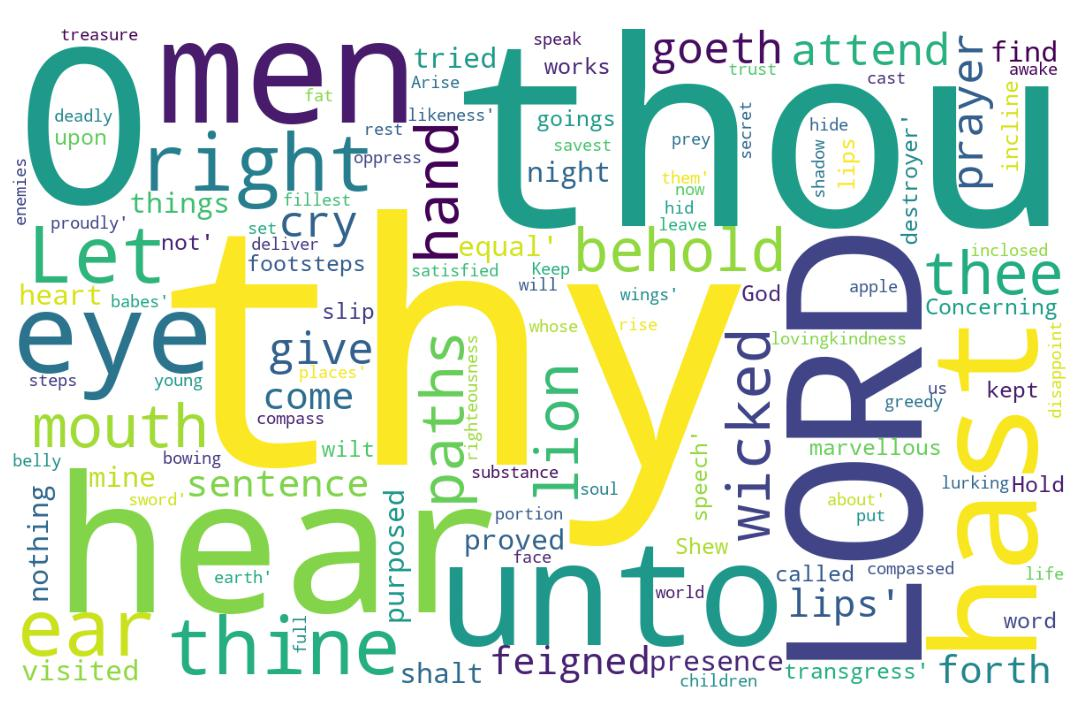
\includegraphics[width=\linewidth]{19OT-Psalms/Psalm17-WordCloud.jpg}
  \caption{Psalm 17 Word Cloud}
  \label{fig:Psalm 17 word Cloud}
\end{figure}


\marginpar{\scriptsize \centering \fcolorbox{bone}{lime}{\textbf{CONFLICTS}}\\ (Psalm 17:1--15) \begin{compactenum}[I.][8]
	\item The \textbf{Presence} of the Lord \index[scripture]{Psalms!Psa 017:01}(Psa 17:1)
	\item The \textbf{Proven} Heart \index[scripture]{Psalms!Psa 017:02}(Psa 17:2)
	\item Upheld \textbf{Paths} of the Wicked \index[scripture]{Psalms!Psa 017:05}(Psa 17:5)
	\item The \textbf{Pride} of Lost Mankind \index[scripture]{Psalms!Psa 017:10}(Psa 17:10)
	\item \textbf{Prey} for the Wicked \index[scripture]{Psalms!Psa 017:12}(Psa 17:12)
	\item The \textbf{Purpose} of the Wicked \index[scripture]{Psalms!Psa 017:13}(Psa 17:13)
	\item The \textbf{Portion} found only in this Life \index[scripture]{Psalms!Psa 017:14}(Psa 17:14)
\end{compactenum}}


\textcolor[cmyk]{0.99998,1,0,0}{A Prayer of David.}\\
\\
\footnote{\textcolor[cmyk]{0.99998,1,0,0}{\hyperlink{TOC}{Return to end of Table of Contents.}}}\footnote{\href{https://audiobible.com/bible/}{\textcolor[cmyk]{0.99998,1,0,0}{Psalms Audio}}}\textcolor[cmyk]{0.99998,1,0,0}{Hear the right,  LORD, attend unto my cry, give ear unto my prayer, \emph{that} \emph{goeth} not out of feigned lips.}\marginpar{\scriptsize \textcolor[rgb]{0.00,0.545,0.269}{$\rightarrow$Things of God (``thy'' used 11 times in chapter): 
\begin{compactenum}
	\item thy face [15],
	\item thy likeness [15],
	\item thy presence [2],
	\item thy lips [4],
	\item thy paths [5],
	\item thy marvelous lovingkindness [7],
	\item thy right hand [7],
	\item thy wings [8],
	\item thy sword [13],
	\item thy hand [14],
	\item thy hid treasure [14],
\end{compactenum}}}
[2] \textcolor[cmyk]{0.99998,1,0,0}{Let \fcolorbox{bone}{lime}{my sentence} come forth from \fcolorbox{bone}{bone}{thy} presence; let thine eyes behold the things that are equal.}
[3] \textcolor[cmyk]{0.99998,1,0,0}{Thou hast proved mine heart; thou hast visited \emph{me} in the night; thou hast tried me, \emph{and} shalt find nothing; I am purposed \emph{that} my mouth shall not transgress.}
[4] \textcolor[cmyk]{0.99998,1,0,0}{Concerning the works of men, by the word of \fcolorbox{bone}{bone}{thy} lips I have kept \emph{me} \emph{from} the paths of the destroyer.}
[5] \textcolor[cmyk]{0.99998,1,0,0}{Hold up \fcolorbox{bone}{lime}{my goings} in \fcolorbox{bone}{bone}{thy} paths, \emph{that} my footsteps slip not.}
[6] \textcolor[cmyk]{0.99998,1,0,0}{I have called upon thee, for thou wilt hear me, O God: incline thine ear unto me, \emph{and} \emph{hear} my speech.}
[7] \textcolor[cmyk]{0.99998,1,0,0}{Shew \fcolorbox{bone}{bone}{thy} marvellous lovingkindness, O thou that savest by \fcolorbox{bone}{bone}{thy} right hand them which put their trust \emph{in} \emph{thee} from those that rise up \emph{against} \emph{them}.}
[8] \textcolor[cmyk]{0.99998,1,0,0}{Keep me as the apple of the eye, hide me under the shadow of \fcolorbox{bone}{bone}{thy} wings,}
[9] \textcolor[cmyk]{0.99998,1,0,0}{From the wicked that oppress me, \emph{from} my deadly enemies, \emph{who} compass me about.}
[10] \textcolor[cmyk]{0.99998,1,0,0}{They are inclosed in their own fat: with their mouth \fcolorbox{bone}{lime}{they speak proudly}.}
[11] \textcolor[cmyk]{0.99998,1,0,0}{They have now compassed us in our steps: they have set their eyes bowing down to the earth;}
[12] \textcolor[cmyk]{0.99998,1,0,0}{Like as a lion \emph{that} is greedy of his \fcolorbox{bone}{lime}{prey}, and as it were a young lion lurking in secret places.}
[13] \textcolor[cmyk]{0.99998,1,0,0}{Arise, O LORD, disappoint him, cast him down: deliver my soul from \fcolorbox{bone}{lime}{the wicked}, \emph{which} \emph{is} \fcolorbox{bone}{bone}{thy} sword:}
[14] \textcolor[cmyk]{0.99998,1,0,0}{From men \emph{which} \emph{are} \fcolorbox{bone}{bone}{thy} hand, O LORD, from men of the world, \emph{which} \emph{have} their \fcolorbox{bone}{lime}{portion} in \emph{this} life, and whose belly thou fillest with \fcolorbox{bone}{bone}{thy} hid \emph{treasure}: they are full of children, and leave the rest of their \emph{substance} to their babes.}
[15] \textcolor[cmyk]{0.99998,1,0,0}{As for me, I will behold \fcolorbox{bone}{bone}{thy} face in \fcolorbox{bone}{MYGOLD}{righteousness}: I shall be satisfied, when I awake, with \fcolorbox{bone}{bone}{thy} likeness.}
\section{Psalm 17 Comments}

\subsection{Numeric Nuggets}
Verse 10 has 13 words. Verse 9 has 13 unique words.One called ``the wicked'' shows up in verse 13.

%\input{19OT-Psalms/Psalm17-WordIndex}
\section{Psalm 17 Outlines}

\subsection{My Outlines}

\subsubsection{Conflict}

\index[speaker]{Keith Anthony!Psalm 017 (Conflict)}
\index[series]{Psalms (Keith Anthony)!Psalm 017 (Conflict)}
\index[date]{2016/06/24!Psalm 017 (Conflict) (Keith Anthony)}
\begin{compactenum}[I.][8]
	\item The \textbf{Presence} of the Lord \index[scripture]{Psalms!Psa 017:01}(Psa 17:1)
	\item The \textbf{Proven} Heart \index[scripture]{Psalms!Psa 017:02}(Psa 17:2)
	\item Upheld \textbf{Paths} of the Wicked \index[scripture]{Psalms!Psa 017:05}(Psa 17:5)
	\item The \textbf{Pride} of Lost Mankind \index[scripture]{Psalms!Psa 017:10}(Psa 17:10)
	\item \textbf{Prey} for the Wicked \index[scripture]{Psalms!Psa 017:12}(Psa 17:12)
	\item The \textbf{Purpose} of the Wicked \index[scripture]{Psalms!Psa 017:13}(Psa 17:13)
	\item The \textbf{Portion} found only in this Life \index[scripture]{Psalms!Psa 017:14}(Psa 17:14)
\end{compactenum}


\subsection{Outlines from Others}


%\section{Psalm 17 Word Statistics}


%%%%%%%%%%
%%%%%%%%%%
\normalsize
 
\begin{center}
\begin{longtable}{l|c|c|c|c}
\caption[Psalm 17 Statistics]{Psalm 17 Statistics}\label{table:Statistics for Psalm 17} \\
\hline \multicolumn{1}{|c|}{\textbf{Verse(s)}} & \multicolumn{1}{|c|}{\textbf{Count}} & \multicolumn{1}{|c|}{\textbf{Unique}} & \multicolumn{1}{|c|}{\textbf{Italics}} & \multicolumn{1}{|c|}{\textbf{Uniq Italic}}  \\ \hline 
\endfirsthead
 
\multicolumn{5}{c}
{{\bfseries \tablename\ \thetable{} -- continued from previous page}} \\  
\hline \multicolumn{1}{|c|}{\textbf{Verse(s)}} & \multicolumn{1}{|c|}{\textbf{Count}} & \multicolumn{1}{|c|}{\textbf{Unique}} & \multicolumn{1}{|c|}{\textbf{Italics}} & \multicolumn{1}{|c|}{\textbf{Uniq Italic}}  \\ \hline 
\endhead
 
\hline \multicolumn{5}{|r|}{{Continued if needed}} \\ \hline
\endfoot 
1 & 20 & 18 & 2 & 2\\ \hline
2 & 17 & 17 & 0 & 0\\ \hline
3 & 29 & 26 & 3 & 3\\ \hline
4 & 21 & 16 & 2 & 2\\ \hline
5 & 12 & 11 & 1 & 1\\ \hline
6 & 21 & 20 & 2 & 2\\ \hline
7 & 26 & 24 & 4 & 4\\ \hline
8 & 16 & 12 & 0 & 0\\ \hline
9 & 14 & 13 & 2 & 2\\ \hline
10 & 13 & 12 & 0 & 0\\ \hline
11 & 18 & 17 & 0 & 0\\ \hline
12 & 21 & 18 & 1 & 1\\ \hline
13 & 18 & 17 & 2 & 2\\ \hline
14 & 44 & 35 & 7 & 6\\ \hline
15 & 20 & 17 & 0 & 0\\ \hline
Total & 310 & 180 & 26 & 18
\end{longtable}
\end{center}



%%%%%%%%%%
%%%%%%%%%%


\subsection{Psalm 17 Words by Frequency}


%%%%%%%%%%
%%%%%%%%%%
\normalsize
 
\begin{center}
\begin{longtable}{l|r}
\caption[Psalm 17 Words by Frequency]{Psalm 17 Words by Frequency}\label{table:WordsbyFrequency for Psalm 17} \\
\hline \multicolumn{1}{|c|}{\textbf{Word}} & \multicolumn{1}{c|}{\textbf{Frequency}} \\ \hline 
\endfirsthead
 
\multicolumn{2}{c}
{{\bfseries \tablename\ \thetable{} -- continued from previous page}} \\  
\hline \multicolumn{1}{|c|}{\textbf{Word}} & \multicolumn{1}{c|}{\textbf{Frequency}} \\ \hline 
\endhead
 
\hline \multicolumn{2}{c}{{ }} \\ \hline
\endfoot 
the & 15\\ \hline 
thy & 11\\ \hline 
of & 10\\ \hline 
my & 9\\ \hline 
me & 8\\ \hline 
in & 7\\ \hline 
their & 7\\ \hline 
I & 6\\ \hline 
thou & 5\\ \hline 
\emph{that} & 4\\ \hline 
from & 4\\ \hline 
that & 4\\ \hline 
have & 4\\ \hline 
O & 4\\ \hline 
LORD & 3\\ \hline 
unto & 3\\ \hline 
not & 3\\ \hline 
are & 3\\ \hline 
hast & 3\\ \hline 
men & 3\\ \hline 
as & 3\\ \hline 
with & 3\\ \hline 
they & 3\\ \hline 
and & 3\\ \hline 
\emph{which} & 3\\ \hline 
right & 2\\ \hline 
ear & 2\\ \hline 
lips & 2\\ \hline 
thine & 2\\ \hline 
eyes & 2\\ \hline 
behold & 2\\ \hline 
\emph{me} & 2\\ \hline 
\emph{and} & 2\\ \hline 
mouth & 2\\ \hline 
shall & 2\\ \hline 
by & 2\\ \hline 
\emph{from} & 2\\ \hline 
paths & 2\\ \hline 
up & 2\\ \hline 
for & 2\\ \hline 
hand & 2\\ \hline 
From & 2\\ \hline 
wicked & 2\\ \hline 
They & 2\\ \hline 
down & 2\\ \hline 
to & 2\\ \hline 
a & 2\\ \hline 
lion & 2\\ \hline 
him & 2\\ \hline 
Hear & 1\\ \hline 
attend & 1\\ \hline 
cry & 1\\ \hline 
give & 1\\ \hline 
prayer & 1\\ \hline 
\emph{goeth} & 1\\ \hline 
out & 1\\ \hline 
feigned & 1\\ \hline 
Let & 1\\ \hline 
sentence & 1\\ \hline 
come & 1\\ \hline 
forth & 1\\ \hline 
presence & 1\\ \hline 
let & 1\\ \hline 
things & 1\\ \hline 
equal & 1\\ \hline 
Thou & 1\\ \hline 
proved & 1\\ \hline 
mine & 1\\ \hline 
heart & 1\\ \hline 
visited & 1\\ \hline 
night & 1\\ \hline 
tried & 1\\ \hline 
shalt & 1\\ \hline 
find & 1\\ \hline 
nothing & 1\\ \hline 
am & 1\\ \hline 
purposed & 1\\ \hline 
transgress & 1\\ \hline 
Concerning & 1\\ \hline 
works & 1\\ \hline 
word & 1\\ \hline 
kept & 1\\ \hline 
destroyer & 1\\ \hline 
Hold & 1\\ \hline 
goings & 1\\ \hline 
footsteps & 1\\ \hline 
slip & 1\\ \hline 
called & 1\\ \hline 
upon & 1\\ \hline 
thee & 1\\ \hline 
wilt & 1\\ \hline 
hear & 1\\ \hline 
God & 1\\ \hline 
incline & 1\\ \hline 
\emph{hear} & 1\\ \hline 
speech & 1\\ \hline 
Shew & 1\\ \hline 
marvellous & 1\\ \hline 
lovingkindness & 1\\ \hline 
savest & 1\\ \hline 
them & 1\\ \hline 
which & 1\\ \hline 
put & 1\\ \hline 
trust & 1\\ \hline 
\emph{in} & 1\\ \hline 
\emph{thee} & 1\\ \hline 
those & 1\\ \hline 
rise & 1\\ \hline 
\emph{against} & 1\\ \hline 
\emph{them} & 1\\ \hline 
Keep & 1\\ \hline 
apple & 1\\ \hline 
eye & 1\\ \hline 
hide & 1\\ \hline 
under & 1\\ \hline 
shadow & 1\\ \hline 
wings & 1\\ \hline 
oppress & 1\\ \hline 
deadly & 1\\ \hline 
enemies & 1\\ \hline 
\emph{who} & 1\\ \hline 
compass & 1\\ \hline 
about & 1\\ \hline 
inclosed & 1\\ \hline 
own & 1\\ \hline 
fat & 1\\ \hline 
speak & 1\\ \hline 
proudly & 1\\ \hline 
now & 1\\ \hline 
compassed & 1\\ \hline 
us & 1\\ \hline 
our & 1\\ \hline 
steps & 1\\ \hline 
set & 1\\ \hline 
bowing & 1\\ \hline 
earth & 1\\ \hline 
Like & 1\\ \hline 
is & 1\\ \hline 
greedy & 1\\ \hline 
his & 1\\ \hline 
prey & 1\\ \hline 
it & 1\\ \hline 
were & 1\\ \hline 
young & 1\\ \hline 
lurking & 1\\ \hline 
secret & 1\\ \hline 
places & 1\\ \hline 
Arise & 1\\ \hline 
disappoint & 1\\ \hline 
cast & 1\\ \hline 
deliver & 1\\ \hline 
soul & 1\\ \hline 
\emph{is} & 1\\ \hline 
sword & 1\\ \hline 
\emph{are} & 1\\ \hline 
world & 1\\ \hline 
\emph{have} & 1\\ \hline 
portion & 1\\ \hline 
\emph{this} & 1\\ \hline 
life & 1\\ \hline 
whose & 1\\ \hline 
belly & 1\\ \hline 
fillest & 1\\ \hline 
hid & 1\\ \hline 
\emph{treasure} & 1\\ \hline 
full & 1\\ \hline 
children & 1\\ \hline 
leave & 1\\ \hline 
rest & 1\\ \hline 
\emph{substance} & 1\\ \hline 
babes & 1\\ \hline 
As & 1\\ \hline 
will & 1\\ \hline 
face & 1\\ \hline 
righteousness & 1\\ \hline 
be & 1\\ \hline 
satisfied & 1\\ \hline 
when & 1\\ \hline 
awake & 1\\ \hline 
likeness & 1\\ \hline 
\end{longtable}
\end{center}



%%%%%%%%%%
%%%%%%%%%%


\subsection{Psalm 17 Words Alphabetically}


%%%%%%%%%%
%%%%%%%%%%
\normalsize
 
\begin{center}
\begin{longtable}{l|r}
\caption[Psalm 17 Words Alphabetically]{Psalm 17 Words Alphabetically}\label{table:WordsAlphabetically for Psalm 17} \\
\hline \multicolumn{1}{|c|}{\textbf{Word}} & \multicolumn{1}{c|}{\textbf{Frequency}} \\ \hline 
\endfirsthead
 
\multicolumn{2}{c}
{{\bfseries \tablename\ \thetable{} -- continued from previous page}} \\  
\hline \multicolumn{1}{|c|}{\textbf{Word}} & \multicolumn{1}{c|}{\textbf{Frequency}} \\ \hline 
\endhead
 
\hline \multicolumn{2}{c}{{ }} \\ \hline
\endfoot 
Arise & 1\\ \hline 
As & 1\\ \hline 
Concerning & 1\\ \hline 
From & 2\\ \hline 
God & 1\\ \hline 
Hear & 1\\ \hline 
Hold & 1\\ \hline 
I & 6\\ \hline 
Keep & 1\\ \hline 
LORD & 3\\ \hline 
Let & 1\\ \hline 
Like & 1\\ \hline 
O & 4\\ \hline 
Shew & 1\\ \hline 
They & 2\\ \hline 
Thou & 1\\ \hline 
\emph{against} & 1\\ \hline 
\emph{and} & 2\\ \hline 
\emph{are} & 1\\ \hline 
\emph{from} & 2\\ \hline 
\emph{goeth} & 1\\ \hline 
\emph{have} & 1\\ \hline 
\emph{hear} & 1\\ \hline 
\emph{in} & 1\\ \hline 
\emph{is} & 1\\ \hline 
\emph{me} & 2\\ \hline 
\emph{substance} & 1\\ \hline 
\emph{that} & 4\\ \hline 
\emph{thee} & 1\\ \hline 
\emph{them} & 1\\ \hline 
\emph{this} & 1\\ \hline 
\emph{treasure} & 1\\ \hline 
\emph{which} & 3\\ \hline 
\emph{who} & 1\\ \hline 
a & 2\\ \hline 
about & 1\\ \hline 
am & 1\\ \hline 
and & 3\\ \hline 
apple & 1\\ \hline 
are & 3\\ \hline 
as & 3\\ \hline 
attend & 1\\ \hline 
awake & 1\\ \hline 
babes & 1\\ \hline 
be & 1\\ \hline 
behold & 2\\ \hline 
belly & 1\\ \hline 
bowing & 1\\ \hline 
by & 2\\ \hline 
called & 1\\ \hline 
cast & 1\\ \hline 
children & 1\\ \hline 
come & 1\\ \hline 
compass & 1\\ \hline 
compassed & 1\\ \hline 
cry & 1\\ \hline 
deadly & 1\\ \hline 
deliver & 1\\ \hline 
destroyer & 1\\ \hline 
disappoint & 1\\ \hline 
down & 2\\ \hline 
ear & 2\\ \hline 
earth & 1\\ \hline 
enemies & 1\\ \hline 
equal & 1\\ \hline 
eye & 1\\ \hline 
eyes & 2\\ \hline 
face & 1\\ \hline 
fat & 1\\ \hline 
feigned & 1\\ \hline 
fillest & 1\\ \hline 
find & 1\\ \hline 
footsteps & 1\\ \hline 
for & 2\\ \hline 
forth & 1\\ \hline 
from & 4\\ \hline 
full & 1\\ \hline 
give & 1\\ \hline 
goings & 1\\ \hline 
greedy & 1\\ \hline 
hand & 2\\ \hline 
hast & 3\\ \hline 
have & 4\\ \hline 
hear & 1\\ \hline 
heart & 1\\ \hline 
hid & 1\\ \hline 
hide & 1\\ \hline 
him & 2\\ \hline 
his & 1\\ \hline 
in & 7\\ \hline 
incline & 1\\ \hline 
inclosed & 1\\ \hline 
is & 1\\ \hline 
it & 1\\ \hline 
kept & 1\\ \hline 
leave & 1\\ \hline 
let & 1\\ \hline 
life & 1\\ \hline 
likeness & 1\\ \hline 
lion & 2\\ \hline 
lips & 2\\ \hline 
lovingkindness & 1\\ \hline 
lurking & 1\\ \hline 
marvellous & 1\\ \hline 
me & 8\\ \hline 
men & 3\\ \hline 
mine & 1\\ \hline 
mouth & 2\\ \hline 
my & 9\\ \hline 
night & 1\\ \hline 
not & 3\\ \hline 
nothing & 1\\ \hline 
now & 1\\ \hline 
of & 10\\ \hline 
oppress & 1\\ \hline 
our & 1\\ \hline 
out & 1\\ \hline 
own & 1\\ \hline 
paths & 2\\ \hline 
places & 1\\ \hline 
portion & 1\\ \hline 
prayer & 1\\ \hline 
presence & 1\\ \hline 
prey & 1\\ \hline 
proudly & 1\\ \hline 
proved & 1\\ \hline 
purposed & 1\\ \hline 
put & 1\\ \hline 
rest & 1\\ \hline 
right & 2\\ \hline 
righteousness & 1\\ \hline 
rise & 1\\ \hline 
satisfied & 1\\ \hline 
savest & 1\\ \hline 
secret & 1\\ \hline 
sentence & 1\\ \hline 
set & 1\\ \hline 
shadow & 1\\ \hline 
shall & 2\\ \hline 
shalt & 1\\ \hline 
slip & 1\\ \hline 
soul & 1\\ \hline 
speak & 1\\ \hline 
speech & 1\\ \hline 
steps & 1\\ \hline 
sword & 1\\ \hline 
that & 4\\ \hline 
the & 15\\ \hline 
thee & 1\\ \hline 
their & 7\\ \hline 
them & 1\\ \hline 
they & 3\\ \hline 
thine & 2\\ \hline 
things & 1\\ \hline 
those & 1\\ \hline 
thou & 5\\ \hline 
thy & 11\\ \hline 
to & 2\\ \hline 
transgress & 1\\ \hline 
tried & 1\\ \hline 
trust & 1\\ \hline 
under & 1\\ \hline 
unto & 3\\ \hline 
up & 2\\ \hline 
upon & 1\\ \hline 
us & 1\\ \hline 
visited & 1\\ \hline 
were & 1\\ \hline 
when & 1\\ \hline 
which & 1\\ \hline 
whose & 1\\ \hline 
wicked & 2\\ \hline 
will & 1\\ \hline 
wilt & 1\\ \hline 
wings & 1\\ \hline 
with & 3\\ \hline 
word & 1\\ \hline 
works & 1\\ \hline 
world & 1\\ \hline 
young & 1\\ \hline 
\end{longtable}
\end{center}



%%%%%%%%%%
%%%%%%%%%%


\subsection{Psalm 17 Words by Length}


%%%%%%%%%%
%%%%%%%%%%
\normalsize
 
\begin{center}
\begin{longtable}{l|p{3.75in}}
\caption[Psalm 17 Words by Length]{Psalm 17 Words by Length}\label{table:WordsAlphabetically for Psalm 17} \\
\hline \multicolumn{1}{|c|}{\textbf{Length}} & \multicolumn{1}{c|}{\textbf{Words}} \\ \hline 
\endfirsthead
\hline \multicolumn{1}{|c|}{\textbf{Length}} & \multicolumn{1}{c|}{\textbf{Words}} \\ \hline 
\multicolumn{2}{c}
{{\bfseries \tablename\ \thetable{} -- continued from previous page}} \\  
\hline \multicolumn{1}{|c|}{\textbf{Word}} & \multicolumn{1}{c|}{\textbf{Frequency}} \\ \hline 
\endhead
 
\hline \multicolumn{2}{c}{{ }} \\ \hline
\endfoot 
1 & I, O, a\\ \hline 
2 & my, of, \emph{me}, in, me, am, by, up, \emph{in}, as, us, to, is, it, \emph{is}, As, be\\ \hline 
3 & the, cry, ear, not, out, Let, thy, let, are, \emph{and}, men, for, God, put, eye, \emph{who}, own, fat, now, our, set, his, and, him, \emph{are}, hid\\ \hline 
4 & Hear, LORD, unto, give, \emph{that}, lips, come, from, eyes, that, Thou, hast, mine, thou, find, word, have, kept, \emph{from}, Hold, slip, upon, thee, wilt, hear, \emph{hear}, Shew, hand, them, \emph{thee}, rise, \emph{them}, Keep, hide, From, They, with, they, down, Like, lion, prey, were, cast, soul, \emph{have}, \emph{this}, life, full, rest, will, face, when\\ \hline 
5 & right, \emph{goeth}, forth, thine, equal, heart, night, tried, shalt, mouth, shall, works, paths, which, their, trust, those, apple, under, wings, about, speak, steps, earth, young, Arise, \emph{which}, sword, world, whose, belly, leave, babes, awake\\ \hline 
6 & attend, prayer, behold, things, proved, goings, called, speech, savest, shadow, wicked, deadly, bowing, greedy, secret, places\\ \hline 
7 & feigned, visited, nothing, incline, \emph{against}, oppress, enemies, compass, proudly, lurking, deliver, portion, fillest\\ \hline 
8 & sentence, presence, purposed, inclosed, \emph{treasure}, children, likeness\\ \hline 
9 & destroyer, footsteps, compassed, \emph{substance}, satisfied\\ \hline 
10 & transgress, Concerning, marvellous, disappoint\\ \hline 
13 & righteousness\\ \hline 
14 & lovingkindness\\ \hline 
\end{longtable}
\end{center}



%%%%%%%%%%
%%%%%%%%%%



\subsection{Psalm 17 Repeated Phrases}


%%%%%%%%%%
%%%%%%%%%%
\normalsize
 
\begin{center}
\begin{longtable}{|p{3.0in}|p{0.5in}|}
\caption[Psalm 17 Repeated Phrases]{Psalm 17 Repeated Phrases}\label{table:Repeated Phrases Psalm 17} \\
\hline \multicolumn{1}{|c|}{\textbf{Phrase}} & \multicolumn{1}{c|}{\textbf{Frequency}} \\ \hline 
\endfirsthead
 
\multicolumn{2}{c}
{{\bfseries \tablename\ \thetable{} -- continued from previous page}} \\  
\hline \multicolumn{1}{|c|}{\textbf{Phrase}} & \multicolumn{1}{c|}{\textbf{Frequency}} \\ \hline 
\endhead
 
\hline \multicolumn{2}{c}{{ }} \\ \hline
\endfoot 
of the & 3\\ \hline 
\end{longtable}
\end{center}



%%%%%%%%%%
%%%%%%%%%%




\chapter{Psalm 18}

\begin{figure}
  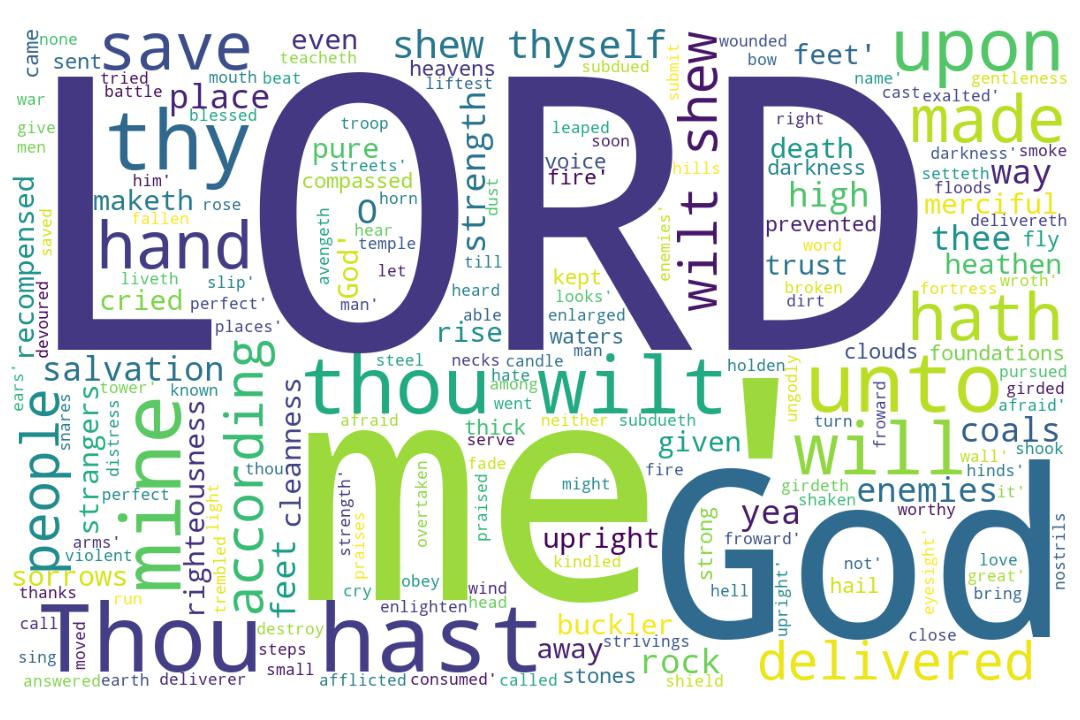
\includegraphics[width=\linewidth]{19OT-Psalms/Psalm18-WordCloud.jpg}
  \caption{Psalm 18 Word Cloud}
  \label{fig:Psalm 18 word Cloud}
\end{figure}

\marginpar{\scriptsize \centering \fcolorbox{bone}{lime}{\textbf{MY SOURCE}}\\ (Psalm 18:1--50) \begin{compactenum}[I.][8]
	\item My Source of \textbf{Strength} \index[scripture]{Psalms!Psa 018:01}(Psalm 18:1, \index[scripture]{Psalms!Psa 018:32}Psa 18:32, \index[scripture]{Psalms!Psa 018:39}Psalm 18:39)
	\item My Source of \textbf{Salvation} \index[scripture]{Psalms!Psa 018:02}(Psa 18:2)
	\item My Source of \textbf{Solace} \index[scripture]{Psalms!Psa 018:06}(Psa 18:6)
	\item My Source of \textbf{Security} \index[scripture]{Psalms!Psa 018:18}(Psa 18:18)
	\item My Source of \textbf{Sympathy} \index[scripture]{Psalms!Psa 018:25}(Psa 18:25)
	\item My Source of \textbf{Skill} \index[scripture]{Psalms!Psa 018:34}(Psa 18:34)
	\item My Source of \textbf{Song} \index[scripture]{Psalms!Psa 018:49}(Psa 18:49)
\end{compactenum}}

\marginpar{\scriptsize \centering \fcolorbox{bone}{yellow}{\textbf{A MAN OF WAR}}\\ (Psalm 18:1--50)\begin{compactenum}[I.][8]
	\item The Lord is a \textbf{Fortress} \index[scripture]{Psalms!Psa 018:02}(Psa 18:2)
	\item The Lord is a \textbf{Deliverer} \index[scripture]{Psalms!Psa 018:02}(Psa 18:2)
	\item The Lord is my \textbf{Strength} \index[scripture]{Psalms!Psa 018:02}(Psa 18:2)
	\item The Lord is a \textbf{Buckler} \index[scripture]{Psalms!Psa 018:02}(Psa 18:2)
	\item The Lord is a \textbf{High Tower} \index[scripture]{Psalms!Psa 018:02}(Psa 18:2)
	\item The Lord is a \textbf{Horn} \index[scripture]{Psalms!Psa 018:02}(Psa 18:2)
	\item The Lord is a \textbf{Rock} \index[scripture]{Numbers!Num 018:02}\index[scripture]{2 Chronicles!2Chr 13:14}\index[scripture]{Psalms!Psa 018:02}(Num 10:2, 2Chr 13:14, Psa 18:2)
\end{compactenum}}

\footnote{\textcolor[cmyk]{0.99998,1,0,0}{\hyperlink{TOC}{Return to end of Table of Contents.}}}\footnote{\href{https://www.audioverse.org/english/audiobibles/books/ENGKJV/O/Ps/1}{\textcolor[cmyk]{0.99998,1,0,0}{Psalms Audio}}}\textcolor[cmyk]{0.99998,1,0,0}{To the chief Musician, \emph{A Psalm} of David, the servant of the LORD, who spake unto the LORD the words of this song in the day \emph{that} the LORD delivered him from the hand of all his enemies, and from the hand of Saul: And he said,}\\
\\
\textcolor[cmyk]{0.99998,1,0,0}{I will love thee, O LORD, \fcolorbox{bone}{lime}{my strength}.}
[2] \textcolor[cmyk]{0.99998,1,0,0}{The LORD \emph{is} my rock, and my fortress, and my deliverer; my God, my strength, in whom I will trust; my buckler, and the \fcolorbox{bone}{lime}{horn of my salvation}, \emph{and} my high tower.}
[3] \textcolor[cmyk]{0.99998,1,0,0}{I will call upon the LORD, \emph{who} \emph{is} \emph{worthy} \fcolorbox{bone}{bone}{to} be praised: so shall I be saved from mine enemies.}
[4] \textcolor[cmyk]{0.99998,1,0,0}{The sorrows of death compassed me, and the floods of ungodly men made me afraid.}
[5] \textcolor[cmyk]{0.99998,1,0,0}{The sorrows of hell compassed me about: the snares of death prevented me.}
[6] \textcolor[cmyk]{0.99998,1,0,0}{In my distress I \fcolorbox{bone}{lime}{called upon the LORD}, and cried unto my God: he heard my voice out of his temple, and my cry came before him, \emph{even} into his ears.}
[7] \textcolor[cmyk]{0.99998,1,0,0}{Then the earth shook and trembled; the foundations also of the hills moved and were shaken, because he was wroth.}
[8] \textcolor[cmyk]{0.99998,1,0,0}{There went up a smoke out of his nostrils, and fire out of his mouth devoured: coals were kindled by it.}
[9] \textcolor[cmyk]{0.99998,1,0,0}{He bowed the heavens also, and came down: and darkness \emph{was} under his feet.}
[10] \textcolor[cmyk]{0.99998,1,0,0}{And he rode upon a cherub, and did fly: yea, he did fly upon the wings of the wind.}
[11] \textcolor[cmyk]{0.99998,1,0,0}{He made darkness his secret place; his pavilion round about him \emph{were} dark waters \emph{and} thick clouds of the skies.}
[12] \textcolor[cmyk]{0.99998,1,0,0}{At the brightness \emph{that} \emph{was} before him his thick clouds passed, hail \emph{stones} and coals of fire.}
[13] \textcolor[cmyk]{0.99998,1,0,0}{The LORD also thundered in the heavens, and the Highest gave his voice; hail \emph{stones} and coals of fire.}\footnote{\textbf{1 Samuel 7:1} - And as Samuel was offering up the burnt offering, the Philistines drew near to battle against Israel: but the LORD thundered with a great thunder on that day upon the Philistines, and discomfited them; and they were smitten before Israel.}\footnote{\textbf{2 Samuel 22:14} -  The LORD thundered from heaven, and the most High uttered his voice.}\footnote{\textbf{John 12:29} - The people therefore, that stood by, and heard it, said that it thundered: others said, An angel spake to him.}
[14] \textcolor[cmyk]{0.99998,1,0,0}{Yea, he sent out his arrows, and scattered them; and he shot out lightnings, and discomfited them.}
[15] \textcolor[cmyk]{0.99998,1,0,0}{Then the channels of waters were seen, and the foundations of the world were discovered at thy rebuke, O LORD, at the blast of the breath of thy nostrils.}
[16] \textcolor[cmyk]{0.99998,1,0,0}{He sent from above, he took me, he drew me out of many waters.}
[17] \textcolor[cmyk]{0.99998,1,0,0}{He delivered me from my strong enemy, and from them which hated me: for they were too strong for me.}
[18] \textcolor[cmyk]{0.99998,1,0,0}{They prevented me in the day of my calamity: but \fcolorbox{bone}{lime}{the LORD was my stay}.}
[19] \textcolor[cmyk]{0.99998,1,0,0}{He brought me forth also into a large place; he delivered me, because he delighted in me.}\footnote{\textbf{2 Samuel 22:20} - He brought me forth also into a large place: he delivered me, because he delighted in me.}\footnote{\textbf{Psalm 118:5} - I called upon the LORD in distress: the LORD answered me, and set me in a large place.}\footnote{\textbf{Hosea 4:16} - For Israel slideth back as a backsliding heifer: now the LORD will feed them as a lamb in a large place.}
[20] \textcolor[cmyk]{0.99998,1,0,0}{The LORD rewarded me according \fcolorbox{bone}{bone}{to} my righteousness; according \fcolorbox{bone}{bone}{to} the cleanness of my hands hath he recompensed me.}
[21] \textcolor[cmyk]{0.99998,1,0,0}{For I have kept the ways of the LORD, and have not wickedly departed from my God.}
[22] \textcolor[cmyk]{0.99998,1,0,0}{For all his judgments \emph{were} before me, and I did not put away his statutes from me.}
[23] \textcolor[cmyk]{0.99998,1,0,0}{I was also upright before him, and I kept myself from mine iniquity.}
[24] \textcolor[cmyk]{0.99998,1,0,0}{Therefore hath the LORD recompensed me according \fcolorbox{bone}{bone}{to} my righteousness, according \fcolorbox{bone}{bone}{to} the cleanness of my hands in his eyesight.}
[25] \textcolor[cmyk]{0.99998,1,0,0}{With the merciful thou wilt \fcolorbox{bone}{lime}{shew thyself merciful}; with an upright man thou wilt shew thyself upright;}
[26] \textcolor[cmyk]{0.99998,1,0,0}{With the pure thou wilt shew thyself pure; and with the froward thou wilt shew thyself froward.}
[27] \textcolor[cmyk]{0.99998,1,0,0}{For thou wilt save the afflicted people; but wilt bring down high looks.}
[28] \textcolor[cmyk]{0.99998,1,0,0}{For thou wilt light my candle: the LORD my God will enlighten my darkness.}
[29] \textcolor[cmyk]{0.99998,1,0,0}{For by thee I have run through a troop; and by my God have I leaped over a wall.}
[30] \textcolor[cmyk]{0.99998,1,0,0}{\emph{As} \emph{for} God, his way \emph{is} perfect: the word of the LORD is tried: he \emph{is} a buckler \fcolorbox{bone}{bone}{to} all those that trust in him.}\footnote{\textbf{Psalm 12:6} - The words of the LORD are pure words: as silver tried in a furnace of earth, purified seven times.}  
[31] \textcolor[cmyk]{0.99998,1,0,0}{For who \emph{is} God save the LORD? or who \emph{is} a rock save our God?}
[32] \textcolor[cmyk]{0.99998,1,0,0}{\emph{It} \emph{is} God that girdeth me with strength, and maketh my way perfect.}
[33] \textcolor[cmyk]{0.99998,1,0,0}{He maketh my feet like hinds' \emph{feet}, and setteth me upon my high places.}
[34] \textcolor[cmyk]{0.99998,1,0,0}{He \fcolorbox{bone}{lime}{teacheth my hands} \fcolorbox{bone}{bone}{to} war, so that a bow of steel is broken by mine arms.}
[35] \textcolor[cmyk]{0.99998,1,0,0}{Thou hast also given me the shield of thy salvation: and thy right hand hath holden me up, and thy gentleness hath made me great.}
[36] \textcolor[cmyk]{0.99998,1,0,0}{Thou hast enlarged my steps under me, that my feet did not slip.}
[37] \textcolor[cmyk]{0.99998,1,0,0}{I have pursued mine enemies, and overtaken them: neither did I turn again till they were consumed.}
[38] \textcolor[cmyk]{0.99998,1,0,0}{I have wounded them that they were not able \fcolorbox{bone}{bone}{to} rise: they are fallen under my feet.}
[39] \textcolor[cmyk]{0.99998,1,0,0}{For thou hast girded me with strength unto the battle: thou hast subdued under me those that rose up against me.}
[40] \textcolor[cmyk]{0.99998,1,0,0}{Thou hast also given me the necks of mine enemies; that I might destroy them that hate me.}
[41] \textcolor[cmyk]{0.99998,1,0,0}{They cried, but \emph{there} \emph{was} none \fcolorbox{bone}{bone}{to} save \emph{them:} \emph{even} unto the LORD, but he answered them not.}
[42] \textcolor[cmyk]{0.99998,1,0,0}{Then did I beat them small as the dust before the wind: I did cast them out as the dirt in the streets.}
[43] \textcolor[cmyk]{0.99998,1,0,0}{Thou hast delivered me from the strivings of the people; \emph{and} thou hast made me the head of the heathen: a people \emph{whom} I have not known shall serve me.}
[44] \textcolor[cmyk]{0.99998,1,0,0}{As soon as they hear of me, they shall obey me: the strangers shall submit themselves unto me.}
[45] \textcolor[cmyk]{0.99998,1,0,0}{The strangers shall fade away, and be afraid out of their close places.}
[46] \textcolor[cmyk]{0.99998,1,0,0}{The LORD liveth; and blessed \emph{be} my rock; and let the God of my salvation be exalted.}
[47] \textcolor[cmyk]{0.99998,1,0,0}{\emph{It} \emph{is} God that avengeth me, and subdueth the people under me.}
[48] \textcolor[cmyk]{0.99998,1,0,0}{He delivereth me from mine enemies: yea, thou liftest me up above those that rise up against me: thou hast delivered me from the violent man.}
[49] \textcolor[cmyk]{0.99998,1,0,0}{Therefore will I give thanks unto thee, O LORD, among the heathen, and \fcolorbox{bone}{lime}{sing praises} unto thy name.}
[50] \textcolor[cmyk]{0.99998,1,0,0}{Great deliverance giveth he \fcolorbox{bone}{bone}{to} his king; and sheweth mercy \fcolorbox{bone}{bone}{to} his anointed, \fcolorbox{bone}{bone}{to} David, and \fcolorbox{bone}{bone}{to} his seed for evermore.}






\section{Psalm 18 Comments}

\subsection{Numeric Nuggets}
Verses 5, 23, 27, 32, 36, and 45 use 13 words. Verses 4, 9, 18, 32, and 45 have 13 unique words. The word ``to'' is used 13 times in the chapter. The 13-letter word ``righteousness'' is found in the chapter.

\subsection{Psalm 18 Introduction}
This psalm is plainly messianic, and it's text parallels that of 2 Samuel 22, with slight variations. Consider this phenomena thoroughly. For example, there are numerous parallel accounts in Matthew, Mark, Luke, and John. Such instances are ripe fields for those who wish to read contradictions into scripture when (1) they do not start out with the assumptions (as we should) of inspiration and infallibility, (2) they (apparently) are not willing to figure out the resolution of these revelations,'' and (3) they cannot admit that they just do not know the answer. Ruckman points out that \cite{Ruckman1992PsalmsV1}:
\begin{compactenum}
    \item Two inspired accounts of the same event do not have to match word for word.
    \item The fact that two words in identical accounts do not match, doe snot mean there is a contradiction in either of them.
    \item A copyist can ``miscopy'' a word, and it still be inspired. Not only is the English text not word for word, but neither is any Massoretic text.
\end{compactenum}

\subsection{Psalm 18:2}
In verse 2, God is likened to seven things, and each of these has a characteristic which is true of Him \cite{Ruckman1992PsalmsV1}:
\begin{compactenum}
\item A Fortress is needed for defensive battle when one is besieged. 
\item A Deliverer is needed in the siege when food is running out.
\item Strength is needed to fight an aggressive warfare.
\item A Buckler is needed to hold your equipment together. 
\item An High Tower is needed for long distance observation.
\item The ``rock'' is the Rock of 1 Corinthians 10:4 and Deuteronomy 32:31. A Rock is needed for a stedfast, immovable foundation upon which to build the fortress. 
\item The seventh item is a ``horn,'' which is needed for mustering the troops to combat (Numbers 10:2), demoralizing the enemy (2 Chronicles 13:14), and celebrating the victory.
\end{compactenum}

\subsection{Psalm 18:4}
See the description of this ``king of terrors'' provided in Job 18:14,\footnote{\textbf{Job 18:14} - His confidence shall be rooted out of his tabernacle, and it shall bring him to the king of terrors.} and, hence, the connection with the book of Job. These ``ungodly men'' are described here, and in 2 Samuel 22:5\footnote{\textbf{2 Samuel 22:5} - When the waves of death compassed me, the floods of ungodly men made me afraid;}, 2 Peter 3:7\footnote{\textbf{2 Peter 3:7} - But the heavens and the earth, which are now, by the same word are kept in store, reserved unto fire against the day of judgment and perdition of ungodly men.}, and Jude 1:4.\footnote{\textbf{Jude 1:4} - For there are certain men crept in unawares, who were before of old ordained to this condemnation, ungodly men, turning the grace of our God into lasciviousness, and denying the only Lord God, and our Lord Jesus Christ.} These ungodly men are described with the attributes of a flood: (1) floods are common, (2) floods move with great speed and power, (3) Floods cannot be stopped, (4) floods have exceptional abilities to destroy lives and property, and (5) floods sweep away existing establishments, burying them. See references to ``a flood'' in scripture: Genesis 6:17, 9:11, 9>15, Job 22:16, Psalm 90:5, Isaiah 28:2, Isaiah 59:19, Jeremiah 46:7-8, Daniel 9:26, Amos 8:8, 9:5, and Revelation 12:5.

\subsection{Psalm 18:7}
Note the context in Revelation 6:12 and Revelation 11:19; it precedes the Advent. ``He bowed the heavens also, and came down'' literally. The Lord told Moses the day this would occur (Exod. 19:11, 18). And this time He will shake heaven and earth, according to Haggai 2:6 and Hebrews 12:25–26. ``He rode upon a cherub,'' so Ezekiel, chapter 1 is a picture of the Advent following the book immediately before it — Lamentations: a picture of the Jews in Uz in the land of Edom (Lam. 4:21). A storm and whirlwind accompany this appearance. ``Dark waters and thick clouds of the skies ... hail stones and coals of fire. The Lord also thundered in the heavens ... hail stones and coals of fire.'' The elements are listed in Job, chapter 37; Matthew 24:27, 29; Revelation 11:13; and Revelation 11:19. The hail stones are a repetition of Joshua 10:11, and that is why the Advent is likened to that battle in Habakkuk 3:7. \cite{Ruckman1992PsalmsV1}

\subsection{Psalm 18:20}
This cannot be the prayer of a Christian, because all of his righteousness is imputed. The same goes for verse 24.

\subsection{Psalm 18:50}
Here is another promotion: our Lord was singing praises to God ``in the midst of the church'' (Heb. 2:12), but now He is singing ``praises unto thy name'' among the heathen. Observe the subtle suggestion in verse 50 that there can be a King beside David. David is a type of ``the King,'' and so David’s seed is a type of Christ’s seed (see Ps. 22:30).\footnote{\textbf{Psalm 22:20} - Deliver my soul from the sword; my darling from the power of the dog.} In the Millennium, Jesus Christ is the King on the Throne of David (Luke 1:30–34), but David is a ``prince'' (Ezek. 44:3) among the people of Israel.\footnote{\textbf{Ezekiel 44:3} - It is for the prince; the prince, he shall sit in it to eat bread before the LORD; he shall enter by the way of the porch of that gate, and shall go out by the way of the same.}\footnote{\textbf{Luke 1:30-34} - And the angel said unto her, Fear not, Mary: for thou hast found favour with God. [31] And, behold, thou shalt conceive in thy womb, and bring forth a son, and shalt call his name JESUS. [32] He shall be great, and shall be called the Son of the Highest: and the Lord God shall give unto him the throne of his father David: [33] And he shall reign over the house of Jacob for ever; and of his kingdom there shall be no end. [34] Then said Mary unto the angel, How shall this be, seeing I know not a man?}\footnote{\textbf{Hebrews 2:12} - Saying, I will declare thy name unto my brethren, in the midst of the church will I sing praise unto thee.} \cite{Ruckman1992PsalmsV1}

%\index[NWIV]{8!Psalms!Psa 18:1}\index[AWIP]{I!Psalms!Psa 18:1}\index[AWIP]{will!Psalms!Psa 18:1}\index[AWIP]{love!Psalms!Psa 18:1}\index[AWIP]{thee!Psalms!Psa 18:1}\index[AWIP]{O!Psalms!Psa 18:1}\index[AWIP]{LORD!Psalms!Psa 18:1}\index[AWIP]{my!Psalms!Psa 18:1}\index[AWIP]{strength!Psalms!Psa 18:1}

\index[NWIV]{32!Psalms!Psa 18:2}\index[AWIP]{The!Psalms!Psa 18:2}\index[AWIP]{LORD!Psalms!Psa 18:2}\index[AWIP]{\emph{is}!Psalms!Psa 18:2}\index[AWIP]{my!Psalms!Psa 18:2}\index[AWIP]{my!Psalms!Psa 18:2 (2)}\index[AWIP]{my!Psalms!Psa 18:2 (3)}\index[AWIP]{my!Psalms!Psa 18:2 (4)}\index[AWIP]{my!Psalms!Psa 18:2 (5)}\index[AWIP]{my!Psalms!Psa 18:2 (6)}\index[AWIP]{my!Psalms!Psa 18:2 (7)}\index[AWIP]{my!Psalms!Psa 18:2 (8)}\index[AWIP]{rock!Psalms!Psa 18:2}\index[AWIP]{and!Psalms!Psa 18:2}\index[AWIP]{and!Psalms!Psa 18:2 (2)}\index[AWIP]{and!Psalms!Psa 18:2 (3)}\index[AWIP]{fortress!Psalms!Psa 18:2}\index[AWIP]{deliverer!Psalms!Psa 18:2}\index[AWIP]{God!Psalms!Psa 18:2}\index[AWIP]{strength!Psalms!Psa 18:2}\index[AWIP]{in!Psalms!Psa 18:2}\index[AWIP]{whom!Psalms!Psa 18:2}\index[AWIP]{I!Psalms!Psa 18:2}\index[AWIP]{will!Psalms!Psa 18:2}\index[AWIP]{trust!Psalms!Psa 18:2}\index[AWIP]{buckler!Psalms!Psa 18:2}\index[AWIP]{the!Psalms!Psa 18:2}\index[AWIP]{horn!Psalms!Psa 18:2}\index[AWIP]{of!Psalms!Psa 18:2}\index[AWIP]{salvation!Psalms!Psa 18:2}\index[AWIP]{\emph{and}!Psalms!Psa 18:2}\index[AWIP]{high!Psalms!Psa 18:2}\index[AWIP]{tower!Psalms!Psa 18:2}\index[AWIP]{\emph{is}!Psalms!Psa 18:2}\index[AWIP]{\emph{and}!Psalms!Psa 18:2}

\index[NWIV]{20!Psalms!Psa 18:3}\index[AWIP]{I!Psalms!Psa 18:3}\index[AWIP]{I!Psalms!Psa 18:3 (2)}\index[AWIP]{will!Psalms!Psa 18:3}\index[AWIP]{call!Psalms!Psa 18:3}\index[AWIP]{upon!Psalms!Psa 18:3}\index[AWIP]{the!Psalms!Psa 18:3}\index[AWIP]{LORD!Psalms!Psa 18:3}\index[AWIP]{\emph{who}!Psalms!Psa 18:3}\index[AWIP]{\emph{is}!Psalms!Psa 18:3}\index[AWIP]{\emph{worthy}!Psalms!Psa 18:3}\index[AWIP]{to!Psalms!Psa 18:3}\index[AWIP]{be!Psalms!Psa 18:3}\index[AWIP]{be!Psalms!Psa 18:3 (2)}\index[AWIP]{praised!Psalms!Psa 18:3}\index[AWIP]{so!Psalms!Psa 18:3}\index[AWIP]{shall!Psalms!Psa 18:3}\index[AWIP]{saved!Psalms!Psa 18:3}\index[AWIP]{from!Psalms!Psa 18:3}\index[AWIP]{mine!Psalms!Psa 18:3}\index[AWIP]{enemies!Psalms!Psa 18:3}\index[AWIP]{\emph{who}!Psalms!Psa 18:3}\index[AWIP]{\emph{is}!Psalms!Psa 18:3}\index[AWIP]{\emph{worthy}!Psalms!Psa 18:3}

\index[NWIV]{15!Psalms!Psa 18:4}\index[AWIP]{The!Psalms!Psa 18:4}\index[AWIP]{sorrows!Psalms!Psa 18:4}\index[AWIP]{of!Psalms!Psa 18:4}\index[AWIP]{of!Psalms!Psa 18:4 (2)}\index[AWIP]{death!Psalms!Psa 18:4}\index[AWIP]{compassed!Psalms!Psa 18:4}\index[AWIP]{me!Psalms!Psa 18:4}\index[AWIP]{me!Psalms!Psa 18:4 (2)}\index[AWIP]{and!Psalms!Psa 18:4}\index[AWIP]{the!Psalms!Psa 18:4}\index[AWIP]{floods!Psalms!Psa 18:4}\index[AWIP]{ungodly!Psalms!Psa 18:4}\index[AWIP]{men!Psalms!Psa 18:4}\index[AWIP]{made!Psalms!Psa 18:4}\index[AWIP]{afraid!Psalms!Psa 18:4}

\index[NWIV]{13!Psalms!Psa 18:5}\index[AWIP]{The!Psalms!Psa 18:5}\index[AWIP]{sorrows!Psalms!Psa 18:5}\index[AWIP]{of!Psalms!Psa 18:5}\index[AWIP]{of!Psalms!Psa 18:5 (2)}\index[AWIP]{hell!Psalms!Psa 18:5}\index[AWIP]{compassed!Psalms!Psa 18:5}\index[AWIP]{me!Psalms!Psa 18:5}\index[AWIP]{me!Psalms!Psa 18:5 (2)}\index[AWIP]{about!Psalms!Psa 18:5}\index[AWIP]{the!Psalms!Psa 18:5}\index[AWIP]{snares!Psalms!Psa 18:5}\index[AWIP]{death!Psalms!Psa 18:5}\index[AWIP]{prevented!Psalms!Psa 18:5}

\index[NWIV]{31!Psalms!Psa 18:6}\index[AWIP]{In!Psalms!Psa 18:6}\index[AWIP]{my!Psalms!Psa 18:6}\index[AWIP]{my!Psalms!Psa 18:6 (2)}\index[AWIP]{my!Psalms!Psa 18:6 (3)}\index[AWIP]{my!Psalms!Psa 18:6 (4)}\index[AWIP]{distress!Psalms!Psa 18:6}\index[AWIP]{I!Psalms!Psa 18:6}\index[AWIP]{called!Psalms!Psa 18:6}\index[AWIP]{upon!Psalms!Psa 18:6}\index[AWIP]{the!Psalms!Psa 18:6}\index[AWIP]{LORD!Psalms!Psa 18:6}\index[AWIP]{and!Psalms!Psa 18:6}\index[AWIP]{and!Psalms!Psa 18:6 (2)}\index[AWIP]{cried!Psalms!Psa 18:6}\index[AWIP]{unto!Psalms!Psa 18:6}\index[AWIP]{God!Psalms!Psa 18:6}\index[AWIP]{he!Psalms!Psa 18:6}\index[AWIP]{heard!Psalms!Psa 18:6}\index[AWIP]{voice!Psalms!Psa 18:6}\index[AWIP]{out!Psalms!Psa 18:6}\index[AWIP]{of!Psalms!Psa 18:6}\index[AWIP]{his!Psalms!Psa 18:6}\index[AWIP]{his!Psalms!Psa 18:6 (2)}\index[AWIP]{temple!Psalms!Psa 18:6}\index[AWIP]{cry!Psalms!Psa 18:6}\index[AWIP]{came!Psalms!Psa 18:6}\index[AWIP]{before!Psalms!Psa 18:6}\index[AWIP]{him!Psalms!Psa 18:6}\index[AWIP]{\emph{even}!Psalms!Psa 18:6}\index[AWIP]{into!Psalms!Psa 18:6}\index[AWIP]{ears!Psalms!Psa 18:6}\index[AWIP]{\emph{even}!Psalms!Psa 18:6}

\index[NWIV]{20!Psalms!Psa 18:7}\index[AWIP]{Then!Psalms!Psa 18:7}\index[AWIP]{the!Psalms!Psa 18:7}\index[AWIP]{the!Psalms!Psa 18:7 (2)}\index[AWIP]{the!Psalms!Psa 18:7 (3)}\index[AWIP]{earth!Psalms!Psa 18:7}\index[AWIP]{shook!Psalms!Psa 18:7}\index[AWIP]{and!Psalms!Psa 18:7}\index[AWIP]{and!Psalms!Psa 18:7 (2)}\index[AWIP]{trembled!Psalms!Psa 18:7}\index[AWIP]{foundations!Psalms!Psa 18:7}\index[AWIP]{also!Psalms!Psa 18:7}\index[AWIP]{of!Psalms!Psa 18:7}\index[AWIP]{hills!Psalms!Psa 18:7}\index[AWIP]{moved!Psalms!Psa 18:7}\index[AWIP]{were!Psalms!Psa 18:7}\index[AWIP]{shaken!Psalms!Psa 18:7}\index[AWIP]{because!Psalms!Psa 18:7}\index[AWIP]{he!Psalms!Psa 18:7}\index[AWIP]{was!Psalms!Psa 18:7}\index[AWIP]{wroth!Psalms!Psa 18:7}

\index[NWIV]{21!Psalms!Psa 18:8}\index[AWIP]{There!Psalms!Psa 18:8}\index[AWIP]{went!Psalms!Psa 18:8}\index[AWIP]{up!Psalms!Psa 18:8}\index[AWIP]{a!Psalms!Psa 18:8}\index[AWIP]{smoke!Psalms!Psa 18:8}\index[AWIP]{out!Psalms!Psa 18:8}\index[AWIP]{out!Psalms!Psa 18:8 (2)}\index[AWIP]{of!Psalms!Psa 18:8}\index[AWIP]{of!Psalms!Psa 18:8 (2)}\index[AWIP]{his!Psalms!Psa 18:8}\index[AWIP]{his!Psalms!Psa 18:8 (2)}\index[AWIP]{nostrils!Psalms!Psa 18:8}\index[AWIP]{and!Psalms!Psa 18:8}\index[AWIP]{fire!Psalms!Psa 18:8}\index[AWIP]{mouth!Psalms!Psa 18:8}\index[AWIP]{devoured!Psalms!Psa 18:8}\index[AWIP]{coals!Psalms!Psa 18:8}\index[AWIP]{were!Psalms!Psa 18:8}\index[AWIP]{kindled!Psalms!Psa 18:8}\index[AWIP]{by!Psalms!Psa 18:8}\index[AWIP]{it!Psalms!Psa 18:8}

\index[NWIV]{14!Psalms!Psa 18:9}\index[AWIP]{He!Psalms!Psa 18:9}\index[AWIP]{bowed!Psalms!Psa 18:9}\index[AWIP]{the!Psalms!Psa 18:9}\index[AWIP]{heavens!Psalms!Psa 18:9}\index[AWIP]{also!Psalms!Psa 18:9}\index[AWIP]{and!Psalms!Psa 18:9}\index[AWIP]{and!Psalms!Psa 18:9 (2)}\index[AWIP]{came!Psalms!Psa 18:9}\index[AWIP]{down!Psalms!Psa 18:9}\index[AWIP]{darkness!Psalms!Psa 18:9}\index[AWIP]{\emph{was}!Psalms!Psa 18:9}\index[AWIP]{under!Psalms!Psa 18:9}\index[AWIP]{his!Psalms!Psa 18:9}\index[AWIP]{feet!Psalms!Psa 18:9}\index[AWIP]{\emph{was}!Psalms!Psa 18:9}

\index[NWIV]{19!Psalms!Psa 18:10}\index[AWIP]{And!Psalms!Psa 18:10}\index[AWIP]{he!Psalms!Psa 18:10}\index[AWIP]{he!Psalms!Psa 18:10 (2)}\index[AWIP]{rode!Psalms!Psa 18:10}\index[AWIP]{upon!Psalms!Psa 18:10}\index[AWIP]{upon!Psalms!Psa 18:10 (2)}\index[AWIP]{a!Psalms!Psa 18:10}\index[AWIP]{cherub!Psalms!Psa 18:10}\index[AWIP]{and!Psalms!Psa 18:10}\index[AWIP]{did!Psalms!Psa 18:10}\index[AWIP]{did!Psalms!Psa 18:10 (2)}\index[AWIP]{fly!Psalms!Psa 18:10}\index[AWIP]{fly!Psalms!Psa 18:10 (2)}\index[AWIP]{yea!Psalms!Psa 18:10}\index[AWIP]{the!Psalms!Psa 18:10}\index[AWIP]{the!Psalms!Psa 18:10 (2)}\index[AWIP]{wings!Psalms!Psa 18:10}\index[AWIP]{of!Psalms!Psa 18:10}\index[AWIP]{wind!Psalms!Psa 18:10}

\index[NWIV]{20!Psalms!Psa 18:11}\index[AWIP]{He!Psalms!Psa 18:11}\index[AWIP]{made!Psalms!Psa 18:11}\index[AWIP]{darkness!Psalms!Psa 18:11}\index[AWIP]{his!Psalms!Psa 18:11}\index[AWIP]{his!Psalms!Psa 18:11 (2)}\index[AWIP]{secret!Psalms!Psa 18:11}\index[AWIP]{place!Psalms!Psa 18:11}\index[AWIP]{pavilion!Psalms!Psa 18:11}\index[AWIP]{round!Psalms!Psa 18:11}\index[AWIP]{about!Psalms!Psa 18:11}\index[AWIP]{him!Psalms!Psa 18:11}\index[AWIP]{\emph{were}!Psalms!Psa 18:11}\index[AWIP]{dark!Psalms!Psa 18:11}\index[AWIP]{waters!Psalms!Psa 18:11}\index[AWIP]{\emph{and}!Psalms!Psa 18:11}\index[AWIP]{thick!Psalms!Psa 18:11}\index[AWIP]{clouds!Psalms!Psa 18:11}\index[AWIP]{of!Psalms!Psa 18:11}\index[AWIP]{the!Psalms!Psa 18:11}\index[AWIP]{skies!Psalms!Psa 18:11}\index[AWIP]{\emph{were}!Psalms!Psa 18:11}\index[AWIP]{\emph{and}!Psalms!Psa 18:11}

\index[NWIV]{17!Psalms!Psa 18:12}\index[AWIP]{At!Psalms!Psa 18:12}\index[AWIP]{the!Psalms!Psa 18:12}\index[AWIP]{brightness!Psalms!Psa 18:12}\index[AWIP]{\emph{that}!Psalms!Psa 18:12}\index[AWIP]{\emph{was}!Psalms!Psa 18:12}\index[AWIP]{before!Psalms!Psa 18:12}\index[AWIP]{him!Psalms!Psa 18:12}\index[AWIP]{his!Psalms!Psa 18:12}\index[AWIP]{thick!Psalms!Psa 18:12}\index[AWIP]{clouds!Psalms!Psa 18:12}\index[AWIP]{passed!Psalms!Psa 18:12}\index[AWIP]{hail!Psalms!Psa 18:12}\index[AWIP]{\emph{stones}!Psalms!Psa 18:12}\index[AWIP]{and!Psalms!Psa 18:12}\index[AWIP]{coals!Psalms!Psa 18:12}\index[AWIP]{of!Psalms!Psa 18:12}\index[AWIP]{fire!Psalms!Psa 18:12}\index[AWIP]{\emph{that}!Psalms!Psa 18:12}\index[AWIP]{\emph{was}!Psalms!Psa 18:12}\index[AWIP]{\emph{stones}!Psalms!Psa 18:12}

\index[NWIV]{19!Psalms!Psa 18:13}\index[AWIP]{The!Psalms!Psa 18:13}\index[AWIP]{LORD!Psalms!Psa 18:13}\index[AWIP]{also!Psalms!Psa 18:13}\index[AWIP]{thundered!Psalms!Psa 18:13}\index[AWIP]{in!Psalms!Psa 18:13}\index[AWIP]{the!Psalms!Psa 18:13}\index[AWIP]{the!Psalms!Psa 18:13 (2)}\index[AWIP]{heavens!Psalms!Psa 18:13}\index[AWIP]{and!Psalms!Psa 18:13}\index[AWIP]{and!Psalms!Psa 18:13 (2)}\index[AWIP]{Highest!Psalms!Psa 18:13}\index[AWIP]{gave!Psalms!Psa 18:13}\index[AWIP]{his!Psalms!Psa 18:13}\index[AWIP]{voice!Psalms!Psa 18:13}\index[AWIP]{hail!Psalms!Psa 18:13}\index[AWIP]{\emph{stones}!Psalms!Psa 18:13}\index[AWIP]{coals!Psalms!Psa 18:13}\index[AWIP]{of!Psalms!Psa 18:13}\index[AWIP]{fire!Psalms!Psa 18:13}\index[AWIP]{\emph{stones}!Psalms!Psa 18:13}

\index[NWIV]{17!Psalms!Psa 18:14}\index[AWIP]{Yea!Psalms!Psa 18:14}\index[AWIP]{he!Psalms!Psa 18:14}\index[AWIP]{he!Psalms!Psa 18:14 (2)}\index[AWIP]{sent!Psalms!Psa 18:14}\index[AWIP]{out!Psalms!Psa 18:14}\index[AWIP]{out!Psalms!Psa 18:14 (2)}\index[AWIP]{his!Psalms!Psa 18:14}\index[AWIP]{arrows!Psalms!Psa 18:14}\index[AWIP]{and!Psalms!Psa 18:14}\index[AWIP]{and!Psalms!Psa 18:14 (2)}\index[AWIP]{and!Psalms!Psa 18:14 (3)}\index[AWIP]{scattered!Psalms!Psa 18:14}\index[AWIP]{them!Psalms!Psa 18:14}\index[AWIP]{them!Psalms!Psa 18:14 (2)}\index[AWIP]{shot!Psalms!Psa 18:14}\index[AWIP]{lightnings!Psalms!Psa 18:14}\index[AWIP]{discomfited!Psalms!Psa 18:14}

\index[NWIV]{29!Psalms!Psa 18:15}\index[AWIP]{Then!Psalms!Psa 18:15}\index[AWIP]{the!Psalms!Psa 18:15}\index[AWIP]{the!Psalms!Psa 18:15 (2)}\index[AWIP]{the!Psalms!Psa 18:15 (3)}\index[AWIP]{the!Psalms!Psa 18:15 (4)}\index[AWIP]{the!Psalms!Psa 18:15 (5)}\index[AWIP]{channels!Psalms!Psa 18:15}\index[AWIP]{of!Psalms!Psa 18:15}\index[AWIP]{of!Psalms!Psa 18:15 (2)}\index[AWIP]{of!Psalms!Psa 18:15 (3)}\index[AWIP]{of!Psalms!Psa 18:15 (4)}\index[AWIP]{waters!Psalms!Psa 18:15}\index[AWIP]{were!Psalms!Psa 18:15}\index[AWIP]{were!Psalms!Psa 18:15 (2)}\index[AWIP]{seen!Psalms!Psa 18:15}\index[AWIP]{and!Psalms!Psa 18:15}\index[AWIP]{foundations!Psalms!Psa 18:15}\index[AWIP]{world!Psalms!Psa 18:15}\index[AWIP]{discovered!Psalms!Psa 18:15}\index[AWIP]{at!Psalms!Psa 18:15}\index[AWIP]{at!Psalms!Psa 18:15 (2)}\index[AWIP]{thy!Psalms!Psa 18:15}\index[AWIP]{thy!Psalms!Psa 18:15 (2)}\index[AWIP]{rebuke!Psalms!Psa 18:15}\index[AWIP]{O!Psalms!Psa 18:15}\index[AWIP]{LORD!Psalms!Psa 18:15}\index[AWIP]{blast!Psalms!Psa 18:15}\index[AWIP]{breath!Psalms!Psa 18:15}\index[AWIP]{nostrils!Psalms!Psa 18:15}

\index[NWIV]{14!Psalms!Psa 18:16}\index[AWIP]{He!Psalms!Psa 18:16}\index[AWIP]{sent!Psalms!Psa 18:16}\index[AWIP]{from!Psalms!Psa 18:16}\index[AWIP]{above!Psalms!Psa 18:16}\index[AWIP]{he!Psalms!Psa 18:16}\index[AWIP]{he!Psalms!Psa 18:16 (2)}\index[AWIP]{took!Psalms!Psa 18:16}\index[AWIP]{me!Psalms!Psa 18:16}\index[AWIP]{me!Psalms!Psa 18:16 (2)}\index[AWIP]{drew!Psalms!Psa 18:16}\index[AWIP]{out!Psalms!Psa 18:16}\index[AWIP]{of!Psalms!Psa 18:16}\index[AWIP]{many!Psalms!Psa 18:16}\index[AWIP]{waters!Psalms!Psa 18:16}

\index[NWIV]{20!Psalms!Psa 18:17}\index[AWIP]{He!Psalms!Psa 18:17}\index[AWIP]{delivered!Psalms!Psa 18:17}\index[AWIP]{me!Psalms!Psa 18:17}\index[AWIP]{me!Psalms!Psa 18:17 (2)}\index[AWIP]{me!Psalms!Psa 18:17 (3)}\index[AWIP]{from!Psalms!Psa 18:17}\index[AWIP]{from!Psalms!Psa 18:17 (2)}\index[AWIP]{my!Psalms!Psa 18:17}\index[AWIP]{strong!Psalms!Psa 18:17}\index[AWIP]{strong!Psalms!Psa 18:17 (2)}\index[AWIP]{enemy!Psalms!Psa 18:17}\index[AWIP]{and!Psalms!Psa 18:17}\index[AWIP]{them!Psalms!Psa 18:17}\index[AWIP]{which!Psalms!Psa 18:17}\index[AWIP]{hated!Psalms!Psa 18:17}\index[AWIP]{for!Psalms!Psa 18:17}\index[AWIP]{for!Psalms!Psa 18:17 (2)}\index[AWIP]{they!Psalms!Psa 18:17}\index[AWIP]{were!Psalms!Psa 18:17}\index[AWIP]{too!Psalms!Psa 18:17}

\index[NWIV]{15!Psalms!Psa 18:18}\index[AWIP]{They!Psalms!Psa 18:18}\index[AWIP]{prevented!Psalms!Psa 18:18}\index[AWIP]{me!Psalms!Psa 18:18}\index[AWIP]{in!Psalms!Psa 18:18}\index[AWIP]{the!Psalms!Psa 18:18}\index[AWIP]{the!Psalms!Psa 18:18 (2)}\index[AWIP]{day!Psalms!Psa 18:18}\index[AWIP]{of!Psalms!Psa 18:18}\index[AWIP]{my!Psalms!Psa 18:18}\index[AWIP]{my!Psalms!Psa 18:18 (2)}\index[AWIP]{calamity!Psalms!Psa 18:18}\index[AWIP]{but!Psalms!Psa 18:18}\index[AWIP]{LORD!Psalms!Psa 18:18}\index[AWIP]{was!Psalms!Psa 18:18}\index[AWIP]{stay!Psalms!Psa 18:18}

\index[NWIV]{17!Psalms!Psa 18:19}\index[AWIP]{He!Psalms!Psa 18:19}\index[AWIP]{brought!Psalms!Psa 18:19}\index[AWIP]{me!Psalms!Psa 18:19}\index[AWIP]{me!Psalms!Psa 18:19 (2)}\index[AWIP]{me!Psalms!Psa 18:19 (3)}\index[AWIP]{forth!Psalms!Psa 18:19}\index[AWIP]{also!Psalms!Psa 18:19}\index[AWIP]{into!Psalms!Psa 18:19}\index[AWIP]{a!Psalms!Psa 18:19}\index[AWIP]{large!Psalms!Psa 18:19}\index[AWIP]{place!Psalms!Psa 18:19}\index[AWIP]{he!Psalms!Psa 18:19}\index[AWIP]{he!Psalms!Psa 18:19 (2)}\index[AWIP]{delivered!Psalms!Psa 18:19}\index[AWIP]{because!Psalms!Psa 18:19}\index[AWIP]{delighted!Psalms!Psa 18:19}\index[AWIP]{in!Psalms!Psa 18:19}

\index[NWIV]{19!Psalms!Psa 18:20}\index[AWIP]{The!Psalms!Psa 18:20}\index[AWIP]{LORD!Psalms!Psa 18:20}\index[AWIP]{rewarded!Psalms!Psa 18:20}\index[AWIP]{me!Psalms!Psa 18:20}\index[AWIP]{me!Psalms!Psa 18:20 (2)}\index[AWIP]{according!Psalms!Psa 18:20}\index[AWIP]{according!Psalms!Psa 18:20 (2)}\index[AWIP]{to!Psalms!Psa 18:20}\index[AWIP]{to!Psalms!Psa 18:20 (2)}\index[AWIP]{my!Psalms!Psa 18:20}\index[AWIP]{my!Psalms!Psa 18:20 (2)}\index[AWIP]{righteousness!Psalms!Psa 18:20}\index[AWIP]{the!Psalms!Psa 18:20}\index[AWIP]{cleanness!Psalms!Psa 18:20}\index[AWIP]{of!Psalms!Psa 18:20}\index[AWIP]{hands!Psalms!Psa 18:20}\index[AWIP]{hath!Psalms!Psa 18:20}\index[AWIP]{he!Psalms!Psa 18:20}\index[AWIP]{recompensed!Psalms!Psa 18:20}

\index[NWIV]{17!Psalms!Psa 18:21}\index[AWIP]{For!Psalms!Psa 18:21}\index[AWIP]{I!Psalms!Psa 18:21}\index[AWIP]{have!Psalms!Psa 18:21}\index[AWIP]{have!Psalms!Psa 18:21 (2)}\index[AWIP]{kept!Psalms!Psa 18:21}\index[AWIP]{the!Psalms!Psa 18:21}\index[AWIP]{the!Psalms!Psa 18:21 (2)}\index[AWIP]{ways!Psalms!Psa 18:21}\index[AWIP]{of!Psalms!Psa 18:21}\index[AWIP]{LORD!Psalms!Psa 18:21}\index[AWIP]{and!Psalms!Psa 18:21}\index[AWIP]{not!Psalms!Psa 18:21}\index[AWIP]{wickedly!Psalms!Psa 18:21}\index[AWIP]{departed!Psalms!Psa 18:21}\index[AWIP]{from!Psalms!Psa 18:21}\index[AWIP]{my!Psalms!Psa 18:21}\index[AWIP]{God!Psalms!Psa 18:21}

\index[NWIV]{17!Psalms!Psa 18:22}\index[AWIP]{For!Psalms!Psa 18:22}\index[AWIP]{all!Psalms!Psa 18:22}\index[AWIP]{his!Psalms!Psa 18:22}\index[AWIP]{his!Psalms!Psa 18:22 (2)}\index[AWIP]{judgments!Psalms!Psa 18:22}\index[AWIP]{\emph{were}!Psalms!Psa 18:22}\index[AWIP]{before!Psalms!Psa 18:22}\index[AWIP]{me!Psalms!Psa 18:22}\index[AWIP]{me!Psalms!Psa 18:22 (2)}\index[AWIP]{and!Psalms!Psa 18:22}\index[AWIP]{I!Psalms!Psa 18:22}\index[AWIP]{did!Psalms!Psa 18:22}\index[AWIP]{not!Psalms!Psa 18:22}\index[AWIP]{put!Psalms!Psa 18:22}\index[AWIP]{away!Psalms!Psa 18:22}\index[AWIP]{statutes!Psalms!Psa 18:22}\index[AWIP]{from!Psalms!Psa 18:22}\index[AWIP]{\emph{were}!Psalms!Psa 18:22}

\index[NWIV]{13!Psalms!Psa 18:23}\index[AWIP]{I!Psalms!Psa 18:23}\index[AWIP]{I!Psalms!Psa 18:23 (2)}\index[AWIP]{was!Psalms!Psa 18:23}\index[AWIP]{also!Psalms!Psa 18:23}\index[AWIP]{upright!Psalms!Psa 18:23}\index[AWIP]{before!Psalms!Psa 18:23}\index[AWIP]{him!Psalms!Psa 18:23}\index[AWIP]{and!Psalms!Psa 18:23}\index[AWIP]{kept!Psalms!Psa 18:23}\index[AWIP]{myself!Psalms!Psa 18:23}\index[AWIP]{from!Psalms!Psa 18:23}\index[AWIP]{mine!Psalms!Psa 18:23}\index[AWIP]{iniquity!Psalms!Psa 18:23}

\index[NWIV]{20!Psalms!Psa 18:24}\index[AWIP]{Therefore!Psalms!Psa 18:24}\index[AWIP]{hath!Psalms!Psa 18:24}\index[AWIP]{the!Psalms!Psa 18:24}\index[AWIP]{the!Psalms!Psa 18:24 (2)}\index[AWIP]{LORD!Psalms!Psa 18:24}\index[AWIP]{recompensed!Psalms!Psa 18:24}\index[AWIP]{me!Psalms!Psa 18:24}\index[AWIP]{according!Psalms!Psa 18:24}\index[AWIP]{according!Psalms!Psa 18:24 (2)}\index[AWIP]{to!Psalms!Psa 18:24}\index[AWIP]{to!Psalms!Psa 18:24 (2)}\index[AWIP]{my!Psalms!Psa 18:24}\index[AWIP]{my!Psalms!Psa 18:24 (2)}\index[AWIP]{righteousness!Psalms!Psa 18:24}\index[AWIP]{cleanness!Psalms!Psa 18:24}\index[AWIP]{of!Psalms!Psa 18:24}\index[AWIP]{hands!Psalms!Psa 18:24}\index[AWIP]{in!Psalms!Psa 18:24}\index[AWIP]{his!Psalms!Psa 18:24}\index[AWIP]{eyesight!Psalms!Psa 18:24}

\index[NWIV]{17!Psalms!Psa 18:25}\index[AWIP]{With!Psalms!Psa 18:25}\index[AWIP]{the!Psalms!Psa 18:25}\index[AWIP]{merciful!Psalms!Psa 18:25}\index[AWIP]{merciful!Psalms!Psa 18:25 (2)}\index[AWIP]{thou!Psalms!Psa 18:25}\index[AWIP]{thou!Psalms!Psa 18:25 (2)}\index[AWIP]{wilt!Psalms!Psa 18:25}\index[AWIP]{wilt!Psalms!Psa 18:25 (2)}\index[AWIP]{shew!Psalms!Psa 18:25}\index[AWIP]{shew!Psalms!Psa 18:25 (2)}\index[AWIP]{thyself!Psalms!Psa 18:25}\index[AWIP]{thyself!Psalms!Psa 18:25 (2)}\index[AWIP]{with!Psalms!Psa 18:25}\index[AWIP]{an!Psalms!Psa 18:25}\index[AWIP]{upright!Psalms!Psa 18:25}\index[AWIP]{upright!Psalms!Psa 18:25 (2)}\index[AWIP]{man!Psalms!Psa 18:25}

\index[NWIV]{17!Psalms!Psa 18:26}\index[AWIP]{With!Psalms!Psa 18:26}\index[AWIP]{the!Psalms!Psa 18:26}\index[AWIP]{the!Psalms!Psa 18:26 (2)}\index[AWIP]{pure!Psalms!Psa 18:26}\index[AWIP]{pure!Psalms!Psa 18:26 (2)}\index[AWIP]{thou!Psalms!Psa 18:26}\index[AWIP]{thou!Psalms!Psa 18:26 (2)}\index[AWIP]{wilt!Psalms!Psa 18:26}\index[AWIP]{wilt!Psalms!Psa 18:26 (2)}\index[AWIP]{shew!Psalms!Psa 18:26}\index[AWIP]{shew!Psalms!Psa 18:26 (2)}\index[AWIP]{thyself!Psalms!Psa 18:26}\index[AWIP]{thyself!Psalms!Psa 18:26 (2)}\index[AWIP]{and!Psalms!Psa 18:26}\index[AWIP]{with!Psalms!Psa 18:26}\index[AWIP]{froward!Psalms!Psa 18:26}\index[AWIP]{froward!Psalms!Psa 18:26 (2)}

\index[NWIV]{13!Psalms!Psa 18:27}\index[AWIP]{For!Psalms!Psa 18:27}\index[AWIP]{thou!Psalms!Psa 18:27}\index[AWIP]{wilt!Psalms!Psa 18:27}\index[AWIP]{wilt!Psalms!Psa 18:27 (2)}\index[AWIP]{save!Psalms!Psa 18:27}\index[AWIP]{the!Psalms!Psa 18:27}\index[AWIP]{afflicted!Psalms!Psa 18:27}\index[AWIP]{people!Psalms!Psa 18:27}\index[AWIP]{but!Psalms!Psa 18:27}\index[AWIP]{bring!Psalms!Psa 18:27}\index[AWIP]{down!Psalms!Psa 18:27}\index[AWIP]{high!Psalms!Psa 18:27}\index[AWIP]{looks!Psalms!Psa 18:27}

\index[NWIV]{14!Psalms!Psa 18:28}\index[AWIP]{For!Psalms!Psa 18:28}\index[AWIP]{thou!Psalms!Psa 18:28}\index[AWIP]{wilt!Psalms!Psa 18:28}\index[AWIP]{light!Psalms!Psa 18:28}\index[AWIP]{my!Psalms!Psa 18:28}\index[AWIP]{my!Psalms!Psa 18:28 (2)}\index[AWIP]{my!Psalms!Psa 18:28 (3)}\index[AWIP]{candle!Psalms!Psa 18:28}\index[AWIP]{the!Psalms!Psa 18:28}\index[AWIP]{LORD!Psalms!Psa 18:28}\index[AWIP]{God!Psalms!Psa 18:28}\index[AWIP]{will!Psalms!Psa 18:28}\index[AWIP]{enlighten!Psalms!Psa 18:28}\index[AWIP]{darkness!Psalms!Psa 18:28}

\index[NWIV]{19!Psalms!Psa 18:29}\index[AWIP]{For!Psalms!Psa 18:29}\index[AWIP]{by!Psalms!Psa 18:29}\index[AWIP]{by!Psalms!Psa 18:29 (2)}\index[AWIP]{thee!Psalms!Psa 18:29}\index[AWIP]{I!Psalms!Psa 18:29}\index[AWIP]{I!Psalms!Psa 18:29 (2)}\index[AWIP]{have!Psalms!Psa 18:29}\index[AWIP]{have!Psalms!Psa 18:29 (2)}\index[AWIP]{run!Psalms!Psa 18:29}\index[AWIP]{through!Psalms!Psa 18:29}\index[AWIP]{a!Psalms!Psa 18:29}\index[AWIP]{a!Psalms!Psa 18:29 (2)}\index[AWIP]{troop!Psalms!Psa 18:29}\index[AWIP]{and!Psalms!Psa 18:29}\index[AWIP]{my!Psalms!Psa 18:29}\index[AWIP]{God!Psalms!Psa 18:29}\index[AWIP]{leaped!Psalms!Psa 18:29}\index[AWIP]{over!Psalms!Psa 18:29}\index[AWIP]{wall!Psalms!Psa 18:29}

\index[NWIV]{25!Psalms!Psa 18:30}\index[AWIP]{\emph{As}!Psalms!Psa 18:30}\index[AWIP]{\emph{for}!Psalms!Psa 18:30}\index[AWIP]{God!Psalms!Psa 18:30}\index[AWIP]{his!Psalms!Psa 18:30}\index[AWIP]{way!Psalms!Psa 18:30}\index[AWIP]{\emph{is}!Psalms!Psa 18:30}\index[AWIP]{\emph{is}!Psalms!Psa 18:30 (2)}\index[AWIP]{perfect!Psalms!Psa 18:30}\index[AWIP]{the!Psalms!Psa 18:30}\index[AWIP]{the!Psalms!Psa 18:30 (2)}\index[AWIP]{word!Psalms!Psa 18:30}\index[AWIP]{of!Psalms!Psa 18:30}\index[AWIP]{LORD!Psalms!Psa 18:30}\index[AWIP]{is!Psalms!Psa 18:30}\index[AWIP]{tried!Psalms!Psa 18:30}\index[AWIP]{he!Psalms!Psa 18:30}\index[AWIP]{a!Psalms!Psa 18:30}\index[AWIP]{buckler!Psalms!Psa 18:30}\index[AWIP]{to!Psalms!Psa 18:30}\index[AWIP]{all!Psalms!Psa 18:30}\index[AWIP]{those!Psalms!Psa 18:30}\index[AWIP]{that!Psalms!Psa 18:30}\index[AWIP]{trust!Psalms!Psa 18:30}\index[AWIP]{in!Psalms!Psa 18:30}\index[AWIP]{him!Psalms!Psa 18:30}\index[AWIP]{\emph{As}!Psalms!Psa 18:30}\index[AWIP]{\emph{for}!Psalms!Psa 18:30}\index[AWIP]{\emph{is}!Psalms!Psa 18:30}\index[AWIP]{\emph{is}!Psalms!Psa 18:30 (2)}

\index[NWIV]{15!Psalms!Psa 18:31}\index[AWIP]{For!Psalms!Psa 18:31}\index[AWIP]{who!Psalms!Psa 18:31}\index[AWIP]{who!Psalms!Psa 18:31 (2)}\index[AWIP]{\emph{is}!Psalms!Psa 18:31}\index[AWIP]{\emph{is}!Psalms!Psa 18:31 (2)}\index[AWIP]{God!Psalms!Psa 18:31}\index[AWIP]{save!Psalms!Psa 18:31}\index[AWIP]{save!Psalms!Psa 18:31 (2)}\index[AWIP]{the!Psalms!Psa 18:31}\index[AWIP]{LORD?!Psalms!Psa 18:31}\index[AWIP]{or!Psalms!Psa 18:31}\index[AWIP]{a!Psalms!Psa 18:31}\index[AWIP]{rock!Psalms!Psa 18:31}\index[AWIP]{our!Psalms!Psa 18:31}\index[AWIP]{God?!Psalms!Psa 18:31}\index[AWIP]{\emph{is}!Psalms!Psa 18:31}\index[AWIP]{\emph{is}!Psalms!Psa 18:31 (2)}

\index[NWIV]{13!Psalms!Psa 18:32}\index[AWIP]{\emph{It}!Psalms!Psa 18:32}\index[AWIP]{\emph{is}!Psalms!Psa 18:32}\index[AWIP]{God!Psalms!Psa 18:32}\index[AWIP]{that!Psalms!Psa 18:32}\index[AWIP]{girdeth!Psalms!Psa 18:32}\index[AWIP]{me!Psalms!Psa 18:32}\index[AWIP]{with!Psalms!Psa 18:32}\index[AWIP]{strength!Psalms!Psa 18:32}\index[AWIP]{and!Psalms!Psa 18:32}\index[AWIP]{maketh!Psalms!Psa 18:32}\index[AWIP]{my!Psalms!Psa 18:32}\index[AWIP]{way!Psalms!Psa 18:32}\index[AWIP]{perfect!Psalms!Psa 18:32}\index[AWIP]{\emph{It}!Psalms!Psa 18:32}\index[AWIP]{\emph{is}!Psalms!Psa 18:32}

\index[NWIV]{14!Psalms!Psa 18:33}\index[AWIP]{He!Psalms!Psa 18:33}\index[AWIP]{maketh!Psalms!Psa 18:33}\index[AWIP]{my!Psalms!Psa 18:33}\index[AWIP]{my!Psalms!Psa 18:33 (2)}\index[AWIP]{feet!Psalms!Psa 18:33}\index[AWIP]{like!Psalms!Psa 18:33}\index[AWIP]{hinds'!Psalms!Psa 18:33}\index[AWIP]{\emph{feet}!Psalms!Psa 18:33}\index[AWIP]{and!Psalms!Psa 18:33}\index[AWIP]{setteth!Psalms!Psa 18:33}\index[AWIP]{me!Psalms!Psa 18:33}\index[AWIP]{upon!Psalms!Psa 18:33}\index[AWIP]{high!Psalms!Psa 18:33}\index[AWIP]{places!Psalms!Psa 18:33}\index[AWIP]{\emph{feet}!Psalms!Psa 18:33}

\index[NWIV]{17!Psalms!Psa 18:34}\index[AWIP]{He!Psalms!Psa 18:34}\index[AWIP]{teacheth!Psalms!Psa 18:34}\index[AWIP]{my!Psalms!Psa 18:34}\index[AWIP]{hands!Psalms!Psa 18:34}\index[AWIP]{to!Psalms!Psa 18:34}\index[AWIP]{war!Psalms!Psa 18:34}\index[AWIP]{so!Psalms!Psa 18:34}\index[AWIP]{that!Psalms!Psa 18:34}\index[AWIP]{a!Psalms!Psa 18:34}\index[AWIP]{bow!Psalms!Psa 18:34}\index[AWIP]{of!Psalms!Psa 18:34}\index[AWIP]{steel!Psalms!Psa 18:34}\index[AWIP]{is!Psalms!Psa 18:34}\index[AWIP]{broken!Psalms!Psa 18:34}\index[AWIP]{by!Psalms!Psa 18:34}\index[AWIP]{mine!Psalms!Psa 18:34}\index[AWIP]{arms!Psalms!Psa 18:34}

\index[NWIV]{25!Psalms!Psa 18:35}\index[AWIP]{Thou!Psalms!Psa 18:35}\index[AWIP]{hast!Psalms!Psa 18:35}\index[AWIP]{also!Psalms!Psa 18:35}\index[AWIP]{given!Psalms!Psa 18:35}\index[AWIP]{me!Psalms!Psa 18:35}\index[AWIP]{me!Psalms!Psa 18:35 (2)}\index[AWIP]{me!Psalms!Psa 18:35 (3)}\index[AWIP]{the!Psalms!Psa 18:35}\index[AWIP]{shield!Psalms!Psa 18:35}\index[AWIP]{of!Psalms!Psa 18:35}\index[AWIP]{thy!Psalms!Psa 18:35}\index[AWIP]{thy!Psalms!Psa 18:35 (2)}\index[AWIP]{thy!Psalms!Psa 18:35 (3)}\index[AWIP]{salvation!Psalms!Psa 18:35}\index[AWIP]{and!Psalms!Psa 18:35}\index[AWIP]{and!Psalms!Psa 18:35 (2)}\index[AWIP]{right!Psalms!Psa 18:35}\index[AWIP]{hand!Psalms!Psa 18:35}\index[AWIP]{hath!Psalms!Psa 18:35}\index[AWIP]{hath!Psalms!Psa 18:35 (2)}\index[AWIP]{holden!Psalms!Psa 18:35}\index[AWIP]{up!Psalms!Psa 18:35}\index[AWIP]{gentleness!Psalms!Psa 18:35}\index[AWIP]{made!Psalms!Psa 18:35}\index[AWIP]{great!Psalms!Psa 18:35}

\index[NWIV]{13!Psalms!Psa 18:36}\index[AWIP]{Thou!Psalms!Psa 18:36}\index[AWIP]{hast!Psalms!Psa 18:36}\index[AWIP]{enlarged!Psalms!Psa 18:36}\index[AWIP]{my!Psalms!Psa 18:36}\index[AWIP]{my!Psalms!Psa 18:36 (2)}\index[AWIP]{steps!Psalms!Psa 18:36}\index[AWIP]{under!Psalms!Psa 18:36}\index[AWIP]{me!Psalms!Psa 18:36}\index[AWIP]{that!Psalms!Psa 18:36}\index[AWIP]{feet!Psalms!Psa 18:36}\index[AWIP]{did!Psalms!Psa 18:36}\index[AWIP]{not!Psalms!Psa 18:36}\index[AWIP]{slip!Psalms!Psa 18:36}

\index[NWIV]{17!Psalms!Psa 18:37}\index[AWIP]{I!Psalms!Psa 18:37}\index[AWIP]{I!Psalms!Psa 18:37 (2)}\index[AWIP]{have!Psalms!Psa 18:37}\index[AWIP]{pursued!Psalms!Psa 18:37}\index[AWIP]{mine!Psalms!Psa 18:37}\index[AWIP]{enemies!Psalms!Psa 18:37}\index[AWIP]{and!Psalms!Psa 18:37}\index[AWIP]{overtaken!Psalms!Psa 18:37}\index[AWIP]{them!Psalms!Psa 18:37}\index[AWIP]{neither!Psalms!Psa 18:37}\index[AWIP]{did!Psalms!Psa 18:37}\index[AWIP]{turn!Psalms!Psa 18:37}\index[AWIP]{again!Psalms!Psa 18:37}\index[AWIP]{till!Psalms!Psa 18:37}\index[AWIP]{they!Psalms!Psa 18:37}\index[AWIP]{were!Psalms!Psa 18:37}\index[AWIP]{consumed!Psalms!Psa 18:37}

\index[NWIV]{17!Psalms!Psa 18:38}\index[AWIP]{I!Psalms!Psa 18:38}\index[AWIP]{have!Psalms!Psa 18:38}\index[AWIP]{wounded!Psalms!Psa 18:38}\index[AWIP]{them!Psalms!Psa 18:38}\index[AWIP]{that!Psalms!Psa 18:38}\index[AWIP]{they!Psalms!Psa 18:38}\index[AWIP]{they!Psalms!Psa 18:38 (2)}\index[AWIP]{were!Psalms!Psa 18:38}\index[AWIP]{not!Psalms!Psa 18:38}\index[AWIP]{able!Psalms!Psa 18:38}\index[AWIP]{to!Psalms!Psa 18:38}\index[AWIP]{rise!Psalms!Psa 18:38}\index[AWIP]{are!Psalms!Psa 18:38}\index[AWIP]{fallen!Psalms!Psa 18:38}\index[AWIP]{under!Psalms!Psa 18:38}\index[AWIP]{my!Psalms!Psa 18:38}\index[AWIP]{feet!Psalms!Psa 18:38}

\index[NWIV]{21!Psalms!Psa 18:39}\index[AWIP]{For!Psalms!Psa 18:39}\index[AWIP]{thou!Psalms!Psa 18:39}\index[AWIP]{thou!Psalms!Psa 18:39 (2)}\index[AWIP]{hast!Psalms!Psa 18:39}\index[AWIP]{hast!Psalms!Psa 18:39 (2)}\index[AWIP]{girded!Psalms!Psa 18:39}\index[AWIP]{me!Psalms!Psa 18:39}\index[AWIP]{me!Psalms!Psa 18:39 (2)}\index[AWIP]{me!Psalms!Psa 18:39 (3)}\index[AWIP]{with!Psalms!Psa 18:39}\index[AWIP]{strength!Psalms!Psa 18:39}\index[AWIP]{unto!Psalms!Psa 18:39}\index[AWIP]{the!Psalms!Psa 18:39}\index[AWIP]{battle!Psalms!Psa 18:39}\index[AWIP]{subdued!Psalms!Psa 18:39}\index[AWIP]{under!Psalms!Psa 18:39}\index[AWIP]{those!Psalms!Psa 18:39}\index[AWIP]{that!Psalms!Psa 18:39}\index[AWIP]{rose!Psalms!Psa 18:39}\index[AWIP]{up!Psalms!Psa 18:39}\index[AWIP]{against!Psalms!Psa 18:39}

\index[NWIV]{18!Psalms!Psa 18:40}\index[AWIP]{Thou!Psalms!Psa 18:40}\index[AWIP]{hast!Psalms!Psa 18:40}\index[AWIP]{also!Psalms!Psa 18:40}\index[AWIP]{given!Psalms!Psa 18:40}\index[AWIP]{me!Psalms!Psa 18:40}\index[AWIP]{me!Psalms!Psa 18:40 (2)}\index[AWIP]{the!Psalms!Psa 18:40}\index[AWIP]{necks!Psalms!Psa 18:40}\index[AWIP]{of!Psalms!Psa 18:40}\index[AWIP]{mine!Psalms!Psa 18:40}\index[AWIP]{enemies!Psalms!Psa 18:40}\index[AWIP]{that!Psalms!Psa 18:40}\index[AWIP]{that!Psalms!Psa 18:40 (2)}\index[AWIP]{I!Psalms!Psa 18:40}\index[AWIP]{might!Psalms!Psa 18:40}\index[AWIP]{destroy!Psalms!Psa 18:40}\index[AWIP]{them!Psalms!Psa 18:40}\index[AWIP]{hate!Psalms!Psa 18:40}

\index[NWIV]{18!Psalms!Psa 18:41}\index[AWIP]{They!Psalms!Psa 18:41}\index[AWIP]{cried!Psalms!Psa 18:41}\index[AWIP]{but!Psalms!Psa 18:41}\index[AWIP]{but!Psalms!Psa 18:41 (2)}\index[AWIP]{\emph{there}!Psalms!Psa 18:41}\index[AWIP]{\emph{was}!Psalms!Psa 18:41}\index[AWIP]{none!Psalms!Psa 18:41}\index[AWIP]{to!Psalms!Psa 18:41}\index[AWIP]{save!Psalms!Psa 18:41}\index[AWIP]{\emph{them}!Psalms!Psa 18:41}\index[AWIP]{\emph{even}!Psalms!Psa 18:41}\index[AWIP]{unto!Psalms!Psa 18:41}\index[AWIP]{the!Psalms!Psa 18:41}\index[AWIP]{LORD!Psalms!Psa 18:41}\index[AWIP]{he!Psalms!Psa 18:41}\index[AWIP]{answered!Psalms!Psa 18:41}\index[AWIP]{them!Psalms!Psa 18:41}\index[AWIP]{not!Psalms!Psa 18:41}\index[AWIP]{\emph{there}!Psalms!Psa 18:41}\index[AWIP]{\emph{was}!Psalms!Psa 18:41}\index[AWIP]{\emph{them}!Psalms!Psa 18:41}\index[AWIP]{\emph{even}!Psalms!Psa 18:41}

\index[NWIV]{23!Psalms!Psa 18:42}\index[AWIP]{Then!Psalms!Psa 18:42}\index[AWIP]{did!Psalms!Psa 18:42}\index[AWIP]{did!Psalms!Psa 18:42 (2)}\index[AWIP]{I!Psalms!Psa 18:42}\index[AWIP]{I!Psalms!Psa 18:42 (2)}\index[AWIP]{beat!Psalms!Psa 18:42}\index[AWIP]{them!Psalms!Psa 18:42}\index[AWIP]{them!Psalms!Psa 18:42 (2)}\index[AWIP]{small!Psalms!Psa 18:42}\index[AWIP]{as!Psalms!Psa 18:42}\index[AWIP]{as!Psalms!Psa 18:42 (2)}\index[AWIP]{the!Psalms!Psa 18:42}\index[AWIP]{the!Psalms!Psa 18:42 (2)}\index[AWIP]{the!Psalms!Psa 18:42 (3)}\index[AWIP]{the!Psalms!Psa 18:42 (4)}\index[AWIP]{dust!Psalms!Psa 18:42}\index[AWIP]{before!Psalms!Psa 18:42}\index[AWIP]{wind!Psalms!Psa 18:42}\index[AWIP]{cast!Psalms!Psa 18:42}\index[AWIP]{out!Psalms!Psa 18:42}\index[AWIP]{dirt!Psalms!Psa 18:42}\index[AWIP]{in!Psalms!Psa 18:42}\index[AWIP]{streets!Psalms!Psa 18:42}

\index[NWIV]{30!Psalms!Psa 18:43}\index[AWIP]{Thou!Psalms!Psa 18:43}\index[AWIP]{hast!Psalms!Psa 18:43}\index[AWIP]{hast!Psalms!Psa 18:43 (2)}\index[AWIP]{delivered!Psalms!Psa 18:43}\index[AWIP]{me!Psalms!Psa 18:43}\index[AWIP]{me!Psalms!Psa 18:43 (2)}\index[AWIP]{me!Psalms!Psa 18:43 (3)}\index[AWIP]{from!Psalms!Psa 18:43}\index[AWIP]{the!Psalms!Psa 18:43}\index[AWIP]{the!Psalms!Psa 18:43 (2)}\index[AWIP]{the!Psalms!Psa 18:43 (3)}\index[AWIP]{the!Psalms!Psa 18:43 (4)}\index[AWIP]{strivings!Psalms!Psa 18:43}\index[AWIP]{of!Psalms!Psa 18:43}\index[AWIP]{of!Psalms!Psa 18:43 (2)}\index[AWIP]{people!Psalms!Psa 18:43}\index[AWIP]{people!Psalms!Psa 18:43 (2)}\index[AWIP]{\emph{and}!Psalms!Psa 18:43}\index[AWIP]{thou!Psalms!Psa 18:43}\index[AWIP]{made!Psalms!Psa 18:43}\index[AWIP]{head!Psalms!Psa 18:43}\index[AWIP]{heathen!Psalms!Psa 18:43}\index[AWIP]{a!Psalms!Psa 18:43}\index[AWIP]{\emph{whom}!Psalms!Psa 18:43}\index[AWIP]{I!Psalms!Psa 18:43}\index[AWIP]{have!Psalms!Psa 18:43}\index[AWIP]{not!Psalms!Psa 18:43}\index[AWIP]{known!Psalms!Psa 18:43}\index[AWIP]{shall!Psalms!Psa 18:43}\index[AWIP]{serve!Psalms!Psa 18:43}\index[AWIP]{\emph{and}!Psalms!Psa 18:43}\index[AWIP]{\emph{whom}!Psalms!Psa 18:43}

\index[NWIV]{18!Psalms!Psa 18:44}\index[AWIP]{As!Psalms!Psa 18:44}\index[AWIP]{soon!Psalms!Psa 18:44}\index[AWIP]{as!Psalms!Psa 18:44}\index[AWIP]{they!Psalms!Psa 18:44}\index[AWIP]{they!Psalms!Psa 18:44 (2)}\index[AWIP]{hear!Psalms!Psa 18:44}\index[AWIP]{of!Psalms!Psa 18:44}\index[AWIP]{me!Psalms!Psa 18:44}\index[AWIP]{me!Psalms!Psa 18:44 (2)}\index[AWIP]{me!Psalms!Psa 18:44 (3)}\index[AWIP]{shall!Psalms!Psa 18:44}\index[AWIP]{shall!Psalms!Psa 18:44 (2)}\index[AWIP]{obey!Psalms!Psa 18:44}\index[AWIP]{the!Psalms!Psa 18:44}\index[AWIP]{strangers!Psalms!Psa 18:44}\index[AWIP]{submit!Psalms!Psa 18:44}\index[AWIP]{themselves!Psalms!Psa 18:44}\index[AWIP]{unto!Psalms!Psa 18:44}

\index[NWIV]{13!Psalms!Psa 18:45}\index[AWIP]{The!Psalms!Psa 18:45}\index[AWIP]{strangers!Psalms!Psa 18:45}\index[AWIP]{shall!Psalms!Psa 18:45}\index[AWIP]{fade!Psalms!Psa 18:45}\index[AWIP]{away!Psalms!Psa 18:45}\index[AWIP]{and!Psalms!Psa 18:45}\index[AWIP]{be!Psalms!Psa 18:45}\index[AWIP]{afraid!Psalms!Psa 18:45}\index[AWIP]{out!Psalms!Psa 18:45}\index[AWIP]{of!Psalms!Psa 18:45}\index[AWIP]{their!Psalms!Psa 18:45}\index[AWIP]{close!Psalms!Psa 18:45}\index[AWIP]{places!Psalms!Psa 18:45}

\index[NWIV]{17!Psalms!Psa 18:46}\index[AWIP]{The!Psalms!Psa 18:46}\index[AWIP]{LORD!Psalms!Psa 18:46}\index[AWIP]{liveth!Psalms!Psa 18:46}\index[AWIP]{and!Psalms!Psa 18:46}\index[AWIP]{and!Psalms!Psa 18:46 (2)}\index[AWIP]{blessed!Psalms!Psa 18:46}\index[AWIP]{\emph{be}!Psalms!Psa 18:46}\index[AWIP]{my!Psalms!Psa 18:46}\index[AWIP]{my!Psalms!Psa 18:46 (2)}\index[AWIP]{rock!Psalms!Psa 18:46}\index[AWIP]{let!Psalms!Psa 18:46}\index[AWIP]{the!Psalms!Psa 18:46}\index[AWIP]{God!Psalms!Psa 18:46}\index[AWIP]{of!Psalms!Psa 18:46}\index[AWIP]{salvation!Psalms!Psa 18:46}\index[AWIP]{be!Psalms!Psa 18:46}\index[AWIP]{exalted!Psalms!Psa 18:46}\index[AWIP]{\emph{be}!Psalms!Psa 18:46}

\index[NWIV]{12!Psalms!Psa 18:47}\index[AWIP]{\emph{It}!Psalms!Psa 18:47}\index[AWIP]{\emph{is}!Psalms!Psa 18:47}\index[AWIP]{God!Psalms!Psa 18:47}\index[AWIP]{that!Psalms!Psa 18:47}\index[AWIP]{avengeth!Psalms!Psa 18:47}\index[AWIP]{me!Psalms!Psa 18:47}\index[AWIP]{me!Psalms!Psa 18:47 (2)}\index[AWIP]{and!Psalms!Psa 18:47}\index[AWIP]{subdueth!Psalms!Psa 18:47}\index[AWIP]{the!Psalms!Psa 18:47}\index[AWIP]{people!Psalms!Psa 18:47}\index[AWIP]{under!Psalms!Psa 18:47}\index[AWIP]{\emph{It}!Psalms!Psa 18:47}\index[AWIP]{\emph{is}!Psalms!Psa 18:47}

\index[NWIV]{26!Psalms!Psa 18:48}\index[AWIP]{He!Psalms!Psa 18:48}\index[AWIP]{delivereth!Psalms!Psa 18:48}\index[AWIP]{me!Psalms!Psa 18:48}\index[AWIP]{me!Psalms!Psa 18:48 (2)}\index[AWIP]{me!Psalms!Psa 18:48 (3)}\index[AWIP]{me!Psalms!Psa 18:48 (4)}\index[AWIP]{from!Psalms!Psa 18:48}\index[AWIP]{from!Psalms!Psa 18:48 (2)}\index[AWIP]{mine!Psalms!Psa 18:48}\index[AWIP]{enemies!Psalms!Psa 18:48}\index[AWIP]{yea!Psalms!Psa 18:48}\index[AWIP]{thou!Psalms!Psa 18:48}\index[AWIP]{thou!Psalms!Psa 18:48 (2)}\index[AWIP]{liftest!Psalms!Psa 18:48}\index[AWIP]{up!Psalms!Psa 18:48}\index[AWIP]{up!Psalms!Psa 18:48 (2)}\index[AWIP]{above!Psalms!Psa 18:48}\index[AWIP]{those!Psalms!Psa 18:48}\index[AWIP]{that!Psalms!Psa 18:48}\index[AWIP]{rise!Psalms!Psa 18:48}\index[AWIP]{against!Psalms!Psa 18:48}\index[AWIP]{hast!Psalms!Psa 18:48}\index[AWIP]{delivered!Psalms!Psa 18:48}\index[AWIP]{the!Psalms!Psa 18:48}\index[AWIP]{violent!Psalms!Psa 18:48}\index[AWIP]{man!Psalms!Psa 18:48}

\index[NWIV]{18!Psalms!Psa 18:49}\index[AWIP]{Therefore!Psalms!Psa 18:49}\index[AWIP]{will!Psalms!Psa 18:49}\index[AWIP]{I!Psalms!Psa 18:49}\index[AWIP]{give!Psalms!Psa 18:49}\index[AWIP]{thanks!Psalms!Psa 18:49}\index[AWIP]{unto!Psalms!Psa 18:49}\index[AWIP]{unto!Psalms!Psa 18:49 (2)}\index[AWIP]{thee!Psalms!Psa 18:49}\index[AWIP]{O!Psalms!Psa 18:49}\index[AWIP]{LORD!Psalms!Psa 18:49}\index[AWIP]{among!Psalms!Psa 18:49}\index[AWIP]{the!Psalms!Psa 18:49}\index[AWIP]{heathen!Psalms!Psa 18:49}\index[AWIP]{and!Psalms!Psa 18:49}\index[AWIP]{sing!Psalms!Psa 18:49}\index[AWIP]{praises!Psalms!Psa 18:49}\index[AWIP]{thy!Psalms!Psa 18:49}\index[AWIP]{name!Psalms!Psa 18:49}

\index[NWIV]{21!Psalms!Psa 18:50}\index[AWIP]{Great!Psalms!Psa 18:50}\index[AWIP]{deliverance!Psalms!Psa 18:50}\index[AWIP]{giveth!Psalms!Psa 18:50}\index[AWIP]{he!Psalms!Psa 18:50}\index[AWIP]{to!Psalms!Psa 18:50}\index[AWIP]{to!Psalms!Psa 18:50 (2)}\index[AWIP]{to!Psalms!Psa 18:50 (3)}\index[AWIP]{to!Psalms!Psa 18:50 (4)}\index[AWIP]{his!Psalms!Psa 18:50}\index[AWIP]{his!Psalms!Psa 18:50 (2)}\index[AWIP]{his!Psalms!Psa 18:50 (3)}\index[AWIP]{king!Psalms!Psa 18:50}\index[AWIP]{and!Psalms!Psa 18:50}\index[AWIP]{and!Psalms!Psa 18:50 (2)}\index[AWIP]{sheweth!Psalms!Psa 18:50}\index[AWIP]{mercy!Psalms!Psa 18:50}\index[AWIP]{anointed!Psalms!Psa 18:50}\index[AWIP]{David!Psalms!Psa 18:50}\index[AWIP]{seed!Psalms!Psa 18:50}\index[AWIP]{for!Psalms!Psa 18:50}\index[AWIP]{evermore!Psalms!Psa 18:50}


\section{Psalm 18 Outlines}

\subsection{My Outlines}

\subsubsection{My Source}
%\textbf{Introduction:} Psalm 18: \footnote{24 June 2016, Keith Anthony}
\index[speaker]{Keith Anthony!Psalm 018 (My Source)}
\index[series]{Psalms (Keith Anthony)!Psalm 018 (My Source)}
\index[date]{2016/06/23!Psalm 018 (My Source) (Keith Anthony)}
\begin{compactenum}[I.][8]
	\item My Source of \textbf{Strength} \index[scripture]{Psalms!Psa 018:01}(Psalm 18:1, \index[scripture]{Psalms!Psa 018:32}Psa 18:32, \index[scripture]{Psalms!Psa 018:39}Psalm 18:39)
	\item My Source of \textbf{Salvation} \index[scripture]{Psalms!Psa 018:02}(Psa 18:2)
	\item My Source of \textbf{Solace} \index[scripture]{Psalms!Psa 018:06}(Psa 18:6)
	\item My Source of \textbf{Security} \index[scripture]{Psalms!Psa 018:18}(Psa 18:18)
	\item My Source of \textbf{Sympathy} \index[scripture]{Psalms!Psa 018:25}(Psa 18:25)
	\item My Source of \textbf{Skill} \index[scripture]{Psalms!Psa 018:34}(Psa 18:34)
	\item My Source of \textbf{Song} \index[scripture]{Psalms!Psa 018:49}(Psa 18:49)
\end{compactenum}

\subsubsection{The Lord, A Man of War}
%\textbf{Introduction:} Psalm 18:2.\footnote{24 June 2016, Keith Anthony}
\index[speaker]{Keith Anthony!Psalm 018 (The Lord, A Man of War)}
\index[series]{Psalms (Keith Anthony)!Psalm 018 (The Lord, A Man of War)}
\index[date]{2016/06/23!Psalm 018 (The Lord, A Man of War) (Keith Anthony)}
\begin{compactenum}[I.][8]
	\item The Lord is a \textbf{Fortress} \index[scripture]{Psalms!Psa 018:02}(Psa 18:2)
	\item The Lord is a \textbf{Deliverer} \index[scripture]{Psalms!Psa 018:02}(Psa 18:2)
	\item The Lord is my \textbf{Strength} \index[scripture]{Psalms!Psa 018:02}(Psa 18:2)
	\item The Lord is a \textbf{Buckler} \index[scripture]{Psalms!Psa 018:02}(Psa 18:2)
	\item The Lord is a \textbf{High Tower} \index[scripture]{Psalms!Psa 018:02}(Psa 18:2)
	\item The Lord is a \textbf{Horn} \index[scripture]{Psalms!Psa 018:02}(Psa 18:2)
	\item The Lord is a \textbf{Rock} \index[scripture]{Numbers!Num 018:02}\index[scripture]{2 Chronicles!2Chr 13:14}\index[scripture]{Psalms!Psa 018:02}(Num 10:2, 2Chr 13:14, Psa 18:2)
\end{compactenum}

\subsection{Outlines from Others}


%\section{Psalm 18 Statistics}

%%%%%%%%%%%%%%%%%%%%%%%%%%%
%%%%%Word Statistics
%%%%%%%%%%%%%%%%%%%%%%%%%%%


\normalsize



\subsection{Chapter Word Statistics}


%%%%%%%%%%
%%%%%%%%%%
 
\begin{center}
\begin{longtable}{l|c|c|c|c}
\caption[Stats for Psalm 18]{Stats for Psalm 18} \label{table:Stats for Psalm 18} \\ 
\hline \multicolumn{1}{|c|}{\textbf{Verse(s)}} & \multicolumn{1}{|c|}{\textbf{Count}} & \multicolumn{1}{|c|}{\textbf{Unique}} & \multicolumn{1}{|c|}{\textbf{Italics}} & \multicolumn{1}{|c|}{\textbf{Uniq Italic}}  \\ \hline 
\endfirsthead
 
\multicolumn{5}{c}
{{\bfseries \tablename\ \thetable{} -- continued from previous page}} \\  
\hline \multicolumn{1}{|c|}{\textbf{Verse(s)}} & \multicolumn{1}{|c|}{\textbf{Count}} & \multicolumn{1}{|c|}{\textbf{Unique}} & \multicolumn{1}{|c|}{\textbf{Italics}} & \multicolumn{1}{|c|}{\textbf{Uniq Italic}}  \\ \hline 
\endhead
 
\hline \multicolumn{5}{|r|}{{Continued if needed}} \\ \hline
\endfoot 
1 & 8 & 8 & 0 & 0\\ \hline
2 & 32 & 23 & 2 & 2\\ \hline
3 & 20 & 18 & 3 & 3\\ \hline
4 & 15 & 13 & 0 & 0\\ \hline
5 & 13 & 11 & 0 & 0\\ \hline
6 & 31 & 26 & 1 & 1\\ \hline
7 & 20 & 17 & 0 & 0\\ \hline
8 & 21 & 18 & 0 & 0\\ \hline
9 & 14 & 13 & 1 & 1\\ \hline
10 & 19 & 14 & 0 & 0\\ \hline
11 & 20 & 19 & 2 & 2\\ \hline
12 & 17 & 17 & 3 & 3\\ \hline
13 & 19 & 17 & 1 & 1\\ \hline
14 & 17 & 12 & 0 & 0\\ \hline
15 & 29 & 19 & 0 & 0\\ \hline
16 & 14 & 12 & 0 & 0\\ \hline
17 & 20 & 15 & 0 & 0\\ \hline
18 & 15 & 13 & 0 & 0\\ \hline
19 & 17 & 14 & 0 & 0\\ \hline
20 & 19 & 15 & 0 & 0\\ \hline
21 & 17 & 15 & 0 & 0\\ \hline
22 & 17 & 15 & 1 & 1\\ \hline
23 & 13 & 12 & 0 & 0\\ \hline
24 & 20 & 16 & 0 & 0\\ \hline
25 & 17 & 11 & 0 & 0\\ \hline
26 & 17 & 10 & 0 & 0\\ \hline
27 & 13 & 12 & 0 & 0\\ \hline
28 & 14 & 12 & 0 & 0\\ \hline
29 & 19 & 15 & 0 & 0\\ \hline
30 & 25 & 23 & 4 & 3\\ \hline
31 & 15 & 11 & 2 & 1\\ \hline
32 & 13 & 13 & 2 & 2\\ \hline
33 & 14 & 13 & 1 & 1\\ \hline
34 & 17 & 17 & 0 & 0\\ \hline
35 & 25 & 19 & 0 & 0\\ \hline
36 & 13 & 12 & 0 & 0\\ \hline
37 & 17 & 16 & 0 & 0\\ \hline
38 & 17 & 16 & 0 & 0\\ \hline
39 & 21 & 17 & 0 & 0\\ \hline
40 & 18 & 16 & 0 & 0\\ \hline
41 & 18 & 17 & 4 & 4\\ \hline
42 & 23 & 16 & 0 & 0\\ \hline
43 & 30 & 22 & 2 & 2\\ \hline
44 & 18 & 14 & 0 & 0\\ \hline
45 & 13 & 13 & 0 & 0\\ \hline
46 & 17 & 15 & 1 & 1\\ \hline
47 & 12 & 11 & 2 & 2\\ \hline
48 & 26 & 20 & 0 & 0\\ \hline
49 & 18 & 17 & 0 & 0\\ \hline
50 & 21 & 15 & 0 & 0\\ \hline
\hline \hline
Total & 918 & 330 & 32 & 17



\end{longtable}
\end{center}

%%%%%%%%%%
%%%%%%%%%%
 
\subsection{Words by Frequency}

\begin{center}
\begin{longtable}{l|r}
\caption[Word Frequencies in Psalm 18]{Word Frequencies in Psalm 18} \label{table:WordsIn-Psalm-18} \\ 
\hline \multicolumn{1}{|c|}{\textbf{Word}} & \multicolumn{1}{c|}{\textbf{Frequency}} \\ \hline 
\endfirsthead
 
\multicolumn{2}{c}
{{\bfseries \tablename\ \thetable{} -- continued from previous page}} \\ 
\hline \multicolumn{1}{|c|}{\textbf{Word}} & \multicolumn{1}{c|}{\textbf{Frequency}} \\ \hline 
\endhead
 
\hline \multicolumn{2}{|r|}{{Continued if needed}} \\ \hline
\endfoot
 
\hline \hline
\endlastfoot
the & 52 \\ \hline
me & 41 \\ \hline
and & 37 \\ \hline
my & 34 \\ \hline
of & 31 \\ \hline
I & 19 \\ \hline
his & 17 \\ \hline
LORD & 16 \\ \hline
he & 14 \\ \hline
to & 13 \\ \hline
God & 11 \\ \hline
thou & 11 \\ \hline
from & 10 \\ \hline
that & 10 \\ \hline
a & 9 \\ \hline
them & 9 \\ \hline
\emph{is} & 8 \\ \hline
out & 8 \\ \hline
He & 8 \\ \hline
hast & 8 \\ \hline
The & 7 \\ \hline
in & 7 \\ \hline
also & 7 \\ \hline
were & 7 \\ \hline
did & 7 \\ \hline
For & 7 \\ \hline
have & 7 \\ \hline
wilt & 7 \\ \hline
mine & 6 \\ \hline
unto & 6 \\ \hline
thy & 6 \\ \hline
they & 6 \\ \hline
not & 6 \\ \hline
will & 5 \\ \hline
upon & 5 \\ \hline
shall & 5 \\ \hline
before & 5 \\ \hline
him & 5 \\ \hline
up & 5 \\ \hline
under & 5 \\ \hline
strength & 4 \\ \hline
be & 4 \\ \hline
enemies & 4 \\ \hline
made & 4 \\ \hline
by & 4 \\ \hline
feet & 4 \\ \hline
delivered & 4 \\ \hline
but & 4 \\ \hline
according & 4 \\ \hline
hath & 4 \\ \hline
shew & 4 \\ \hline
thyself & 4 \\ \hline
with & 4 \\ \hline
save & 4 \\ \hline
people & 4 \\ \hline
Thou & 4 \\ \hline
thee & 3 \\ \hline
O & 3 \\ \hline
rock & 3 \\ \hline
salvation & 3 \\ \hline
\emph{and} & 3 \\ \hline
high & 3 \\ \hline
Then & 3 \\ \hline
was & 3 \\ \hline
fire & 3 \\ \hline
coals & 3 \\ \hline
darkness & 3 \\ \hline
\emph{was} & 3 \\ \hline
waters & 3 \\ \hline
for & 3 \\ \hline
hands & 3 \\ \hline
upright & 3 \\ \hline
those & 3 \\ \hline
as & 3 \\ \hline
trust & 2 \\ \hline
buckler & 2 \\ \hline
so & 2 \\ \hline
sorrows & 2 \\ \hline
death & 2 \\ \hline
compassed & 2 \\ \hline
afraid & 2 \\ \hline
about & 2 \\ \hline
prevented & 2 \\ \hline
cried & 2 \\ \hline
voice & 2 \\ \hline
came & 2 \\ \hline
\emph{even} & 2 \\ \hline
into & 2 \\ \hline
foundations & 2 \\ \hline
because & 2 \\ \hline
nostrils & 2 \\ \hline
heavens & 2 \\ \hline
down & 2 \\ \hline
fly & 2 \\ \hline
yea & 2 \\ \hline
wind & 2 \\ \hline
place & 2 \\ \hline
\emph{were} & 2 \\ \hline
thick & 2 \\ \hline
clouds & 2 \\ \hline
hail & 2 \\ \hline
\emph{stones} & 2 \\ \hline
sent & 2 \\ \hline
at & 2 \\ \hline
above & 2 \\ \hline
strong & 2 \\ \hline
They & 2 \\ \hline
righteousness & 2 \\ \hline
cleanness & 2 \\ \hline
recompensed & 2 \\ \hline
kept & 2 \\ \hline
all & 2 \\ \hline
away & 2 \\ \hline
Therefore & 2 \\ \hline
With & 2 \\ \hline
merciful & 2 \\ \hline
man & 2 \\ \hline
pure & 2 \\ \hline
froward & 2 \\ \hline
way & 2 \\ \hline
perfect & 2 \\ \hline
is & 2 \\ \hline
who & 2 \\ \hline
\emph{It} & 2 \\ \hline
maketh & 2 \\ \hline
places & 2 \\ \hline
given & 2 \\ \hline
rise & 2 \\ \hline
against & 2 \\ \hline
heathen & 2 \\ \hline
strangers & 2 \\ \hline
love & 1 \\ \hline
fortress & 1 \\ \hline
deliverer & 1 \\ \hline
whom & 1 \\ \hline
horn & 1 \\ \hline
tower & 1 \\ \hline
call & 1 \\ \hline
\emph{who} & 1 \\ \hline
\emph{worthy} & 1 \\ \hline
praised & 1 \\ \hline
saved & 1 \\ \hline
floods & 1 \\ \hline
ungodly & 1 \\ \hline
men & 1 \\ \hline
hell & 1 \\ \hline
snares & 1 \\ \hline
In & 1 \\ \hline
distress & 1 \\ \hline
called & 1 \\ \hline
heard & 1 \\ \hline
temple & 1 \\ \hline
cry & 1 \\ \hline
ears & 1 \\ \hline
earth & 1 \\ \hline
shook & 1 \\ \hline
trembled & 1 \\ \hline
hills & 1 \\ \hline
moved & 1 \\ \hline
shaken & 1 \\ \hline
wroth & 1 \\ \hline
There & 1 \\ \hline
went & 1 \\ \hline
smoke & 1 \\ \hline
mouth & 1 \\ \hline
devoured & 1 \\ \hline
kindled & 1 \\ \hline
it & 1 \\ \hline
bowed & 1 \\ \hline
And & 1 \\ \hline
rode & 1 \\ \hline
cherub & 1 \\ \hline
wings & 1 \\ \hline
secret & 1 \\ \hline
pavilion & 1 \\ \hline
round & 1 \\ \hline
dark & 1 \\ \hline
skies & 1 \\ \hline
At & 1 \\ \hline
brightness & 1 \\ \hline
\emph{that} & 1 \\ \hline
passed & 1 \\ \hline
thundered & 1 \\ \hline
Highest & 1 \\ \hline
gave & 1 \\ \hline
Yea & 1 \\ \hline
arrows & 1 \\ \hline
scattered & 1 \\ \hline
shot & 1 \\ \hline
lightnings & 1 \\ \hline
discomfited & 1 \\ \hline
channels & 1 \\ \hline
seen & 1 \\ \hline
world & 1 \\ \hline
discovered & 1 \\ \hline
rebuke & 1 \\ \hline
blast & 1 \\ \hline
breath & 1 \\ \hline
took & 1 \\ \hline
drew & 1 \\ \hline
many & 1 \\ \hline
enemy & 1 \\ \hline
which & 1 \\ \hline
hated & 1 \\ \hline
too & 1 \\ \hline
day & 1 \\ \hline
calamity & 1 \\ \hline
stay & 1 \\ \hline
brought & 1 \\ \hline
forth & 1 \\ \hline
large & 1 \\ \hline
delighted & 1 \\ \hline
rewarded & 1 \\ \hline
ways & 1 \\ \hline
wickedly & 1 \\ \hline
departed & 1 \\ \hline
judgments & 1 \\ \hline
put & 1 \\ \hline
statutes & 1 \\ \hline
myself & 1 \\ \hline
iniquity & 1 \\ \hline
eyesight & 1 \\ \hline
an & 1 \\ \hline
afflicted & 1 \\ \hline
bring & 1 \\ \hline
looks & 1 \\ \hline
light & 1 \\ \hline
candle & 1 \\ \hline
enlighten & 1 \\ \hline
run & 1 \\ \hline
through & 1 \\ \hline
troop & 1 \\ \hline
leaped & 1 \\ \hline
over & 1 \\ \hline
wall & 1 \\ \hline
\emph{As} & 1 \\ \hline
\emph{for} & 1 \\ \hline
word & 1 \\ \hline
tried & 1 \\ \hline
or & 1 \\ \hline
our & 1 \\ \hline
girdeth & 1 \\ \hline
like & 1 \\ \hline
hinds' & 1 \\ \hline
\emph{feet} & 1 \\ \hline
setteth & 1 \\ \hline
teacheth & 1 \\ \hline
war & 1 \\ \hline
bow & 1 \\ \hline
steel & 1 \\ \hline
broken & 1 \\ \hline
arms & 1 \\ \hline
shield & 1 \\ \hline
right & 1 \\ \hline
hand & 1 \\ \hline
holden & 1 \\ \hline
gentleness & 1 \\ \hline
great & 1 \\ \hline
enlarged & 1 \\ \hline
steps & 1 \\ \hline
slip & 1 \\ \hline
pursued & 1 \\ \hline
overtaken & 1 \\ \hline
neither & 1 \\ \hline
turn & 1 \\ \hline
again & 1 \\ \hline
till & 1 \\ \hline
consumed & 1 \\ \hline
wounded & 1 \\ \hline
able & 1 \\ \hline
are & 1 \\ \hline
fallen & 1 \\ \hline
girded & 1 \\ \hline
battle & 1 \\ \hline
subdued & 1 \\ \hline
rose & 1 \\ \hline
necks & 1 \\ \hline
might & 1 \\ \hline
destroy & 1 \\ \hline
hate & 1 \\ \hline
\emph{there} & 1 \\ \hline
none & 1 \\ \hline
\emph{them} & 1 \\ \hline
answered & 1 \\ \hline
beat & 1 \\ \hline
small & 1 \\ \hline
dust & 1 \\ \hline
cast & 1 \\ \hline
dirt & 1 \\ \hline
streets & 1 \\ \hline
strivings & 1 \\ \hline
head & 1 \\ \hline
\emph{whom} & 1 \\ \hline
known & 1 \\ \hline
serve & 1 \\ \hline
As & 1 \\ \hline
soon & 1 \\ \hline
hear & 1 \\ \hline
obey & 1 \\ \hline
submit & 1 \\ \hline
themselves & 1 \\ \hline
fade & 1 \\ \hline
their & 1 \\ \hline
close & 1 \\ \hline
liveth & 1 \\ \hline
blessed & 1 \\ \hline
\emph{be} & 1 \\ \hline
let & 1 \\ \hline
exalted & 1 \\ \hline
avengeth & 1 \\ \hline
subdueth & 1 \\ \hline
delivereth & 1 \\ \hline
liftest & 1 \\ \hline
violent & 1 \\ \hline
give & 1 \\ \hline
thanks & 1 \\ \hline
among & 1 \\ \hline
sing & 1 \\ \hline
praises & 1 \\ \hline
name & 1 \\ \hline
Great & 1 \\ \hline
deliverance & 1 \\ \hline
giveth & 1 \\ \hline
king & 1 \\ \hline
sheweth & 1 \\ \hline
mercy & 1 \\ \hline
anointed & 1 \\ \hline
David & 1 \\ \hline
seed & 1 \\ \hline
evermore & 1 \\ \hline
\end{longtable}
\end{center}



\normalsize



\subsection{Words Alphabetically}

\begin{center}
\begin{longtable}{l|r}
\caption[Word Alphabetically in Psalm 18]{Word Alphabetically in Psalm 18} \label{table:WordsIn-Psalm-18} \\ 
\hline \multicolumn{1}{|c|}{\textbf{Word}} & \multicolumn{1}{c|}{\textbf{Frequency}} \\ \hline 
\endfirsthead
 
\multicolumn{2}{c}
{{\bfseries \tablename\ \thetable{} -- continued from previous page}} \\ 
\hline \multicolumn{1}{|c|}{\textbf{Word}} & \multicolumn{1}{c|}{\textbf{Frequency}} \\ \hline 
\endhead
 
\hline \multicolumn{2}{|r|}{{Continued if needed}} \\ \hline
\endfoot
 
\hline \hline
\endlastfoot
And & 1 \\ \hline
As & 1 \\ \hline
At & 1 \\ \hline
David & 1 \\ \hline
For & 7 \\ \hline
God & 11 \\ \hline
Great & 1 \\ \hline
He & 8 \\ \hline
Highest & 1 \\ \hline
I & 19 \\ \hline
In & 1 \\ \hline
LORD & 16 \\ \hline
O & 3 \\ \hline
The & 7 \\ \hline
Then & 3 \\ \hline
There & 1 \\ \hline
Therefore & 2 \\ \hline
They & 2 \\ \hline
Thou & 4 \\ \hline
With & 2 \\ \hline
Yea & 1 \\ \hline
\emph{As} & 1 \\ \hline
\emph{It} & 2 \\ \hline
\emph{and} & 3 \\ \hline
\emph{be} & 1 \\ \hline
\emph{even} & 2 \\ \hline
\emph{feet} & 1 \\ \hline
\emph{for} & 1 \\ \hline
\emph{is} & 8 \\ \hline
\emph{stones} & 2 \\ \hline
\emph{that} & 1 \\ \hline
\emph{them} & 1 \\ \hline
\emph{there} & 1 \\ \hline
\emph{was} & 3 \\ \hline
\emph{were} & 2 \\ \hline
\emph{whom} & 1 \\ \hline
\emph{who} & 1 \\ \hline
\emph{worthy} & 1 \\ \hline
a & 9 \\ \hline
able & 1 \\ \hline
about & 2 \\ \hline
above & 2 \\ \hline
according & 4 \\ \hline
afflicted & 1 \\ \hline
afraid & 2 \\ \hline
again & 1 \\ \hline
against & 2 \\ \hline
all & 2 \\ \hline
also & 7 \\ \hline
among & 1 \\ \hline
an & 1 \\ \hline
and & 37 \\ \hline
anointed & 1 \\ \hline
answered & 1 \\ \hline
are & 1 \\ \hline
arms & 1 \\ \hline
arrows & 1 \\ \hline
as & 3 \\ \hline
at & 2 \\ \hline
avengeth & 1 \\ \hline
away & 2 \\ \hline
battle & 1 \\ \hline
be & 4 \\ \hline
beat & 1 \\ \hline
because & 2 \\ \hline
before & 5 \\ \hline
blast & 1 \\ \hline
blessed & 1 \\ \hline
bow & 1 \\ \hline
bowed & 1 \\ \hline
breath & 1 \\ \hline
brightness & 1 \\ \hline
bring & 1 \\ \hline
broken & 1 \\ \hline
brought & 1 \\ \hline
buckler & 2 \\ \hline
but & 4 \\ \hline
by & 4 \\ \hline
calamity & 1 \\ \hline
call & 1 \\ \hline
called & 1 \\ \hline
came & 2 \\ \hline
candle & 1 \\ \hline
cast & 1 \\ \hline
channels & 1 \\ \hline
cherub & 1 \\ \hline
cleanness & 2 \\ \hline
close & 1 \\ \hline
clouds & 2 \\ \hline
coals & 3 \\ \hline
compassed & 2 \\ \hline
consumed & 1 \\ \hline
cried & 2 \\ \hline
cry & 1 \\ \hline
dark & 1 \\ \hline
darkness & 3 \\ \hline
day & 1 \\ \hline
death & 2 \\ \hline
delighted & 1 \\ \hline
deliverance & 1 \\ \hline
delivered & 4 \\ \hline
deliverer & 1 \\ \hline
delivereth & 1 \\ \hline
departed & 1 \\ \hline
destroy & 1 \\ \hline
devoured & 1 \\ \hline
did & 7 \\ \hline
dirt & 1 \\ \hline
discomfited & 1 \\ \hline
discovered & 1 \\ \hline
distress & 1 \\ \hline
down & 2 \\ \hline
drew & 1 \\ \hline
dust & 1 \\ \hline
ears & 1 \\ \hline
earth & 1 \\ \hline
enemies & 4 \\ \hline
enemy & 1 \\ \hline
enlarged & 1 \\ \hline
enlighten & 1 \\ \hline
evermore & 1 \\ \hline
exalted & 1 \\ \hline
eyesight & 1 \\ \hline
fade & 1 \\ \hline
fallen & 1 \\ \hline
feet & 4 \\ \hline
fire & 3 \\ \hline
floods & 1 \\ \hline
fly & 2 \\ \hline
for & 3 \\ \hline
forth & 1 \\ \hline
fortress & 1 \\ \hline
foundations & 2 \\ \hline
from & 10 \\ \hline
froward & 2 \\ \hline
gave & 1 \\ \hline
gentleness & 1 \\ \hline
girded & 1 \\ \hline
girdeth & 1 \\ \hline
give & 1 \\ \hline
given & 2 \\ \hline
giveth & 1 \\ \hline
great & 1 \\ \hline
hail & 2 \\ \hline
hand & 1 \\ \hline
hands & 3 \\ \hline
hast & 8 \\ \hline
hate & 1 \\ \hline
hated & 1 \\ \hline
hath & 4 \\ \hline
have & 7 \\ \hline
he & 14 \\ \hline
head & 1 \\ \hline
hear & 1 \\ \hline
heard & 1 \\ \hline
heathen & 2 \\ \hline
heavens & 2 \\ \hline
hell & 1 \\ \hline
high & 3 \\ \hline
hills & 1 \\ \hline
him & 5 \\ \hline
hinds' & 1 \\ \hline
his & 17 \\ \hline
holden & 1 \\ \hline
horn & 1 \\ \hline
in & 7 \\ \hline
iniquity & 1 \\ \hline
into & 2 \\ \hline
is & 2 \\ \hline
it & 1 \\ \hline
judgments & 1 \\ \hline
kept & 2 \\ \hline
kindled & 1 \\ \hline
king & 1 \\ \hline
known & 1 \\ \hline
large & 1 \\ \hline
leaped & 1 \\ \hline
let & 1 \\ \hline
liftest & 1 \\ \hline
light & 1 \\ \hline
lightnings & 1 \\ \hline
like & 1 \\ \hline
liveth & 1 \\ \hline
looks & 1 \\ \hline
love & 1 \\ \hline
made & 4 \\ \hline
maketh & 2 \\ \hline
man & 2 \\ \hline
many & 1 \\ \hline
me & 41 \\ \hline
men & 1 \\ \hline
merciful & 2 \\ \hline
mercy & 1 \\ \hline
might & 1 \\ \hline
mine & 6 \\ \hline
mouth & 1 \\ \hline
moved & 1 \\ \hline
my & 34 \\ \hline
myself & 1 \\ \hline
name & 1 \\ \hline
necks & 1 \\ \hline
neither & 1 \\ \hline
none & 1 \\ \hline
nostrils & 2 \\ \hline
not & 6 \\ \hline
obey & 1 \\ \hline
of & 31 \\ \hline
or & 1 \\ \hline
our & 1 \\ \hline
out & 8 \\ \hline
over & 1 \\ \hline
overtaken & 1 \\ \hline
passed & 1 \\ \hline
pavilion & 1 \\ \hline
people & 4 \\ \hline
perfect & 2 \\ \hline
place & 2 \\ \hline
places & 2 \\ \hline
praised & 1 \\ \hline
praises & 1 \\ \hline
prevented & 2 \\ \hline
pure & 2 \\ \hline
pursued & 1 \\ \hline
put & 1 \\ \hline
rebuke & 1 \\ \hline
recompensed & 2 \\ \hline
rewarded & 1 \\ \hline
right & 1 \\ \hline
righteousness & 2 \\ \hline
rise & 2 \\ \hline
rock & 3 \\ \hline
rode & 1 \\ \hline
rose & 1 \\ \hline
round & 1 \\ \hline
run & 1 \\ \hline
salvation & 3 \\ \hline
save & 4 \\ \hline
saved & 1 \\ \hline
scattered & 1 \\ \hline
secret & 1 \\ \hline
seed & 1 \\ \hline
seen & 1 \\ \hline
sent & 2 \\ \hline
serve & 1 \\ \hline
setteth & 1 \\ \hline
shaken & 1 \\ \hline
shall & 5 \\ \hline
shew & 4 \\ \hline
sheweth & 1 \\ \hline
shield & 1 \\ \hline
shook & 1 \\ \hline
shot & 1 \\ \hline
sing & 1 \\ \hline
skies & 1 \\ \hline
slip & 1 \\ \hline
small & 1 \\ \hline
smoke & 1 \\ \hline
snares & 1 \\ \hline
so & 2 \\ \hline
soon & 1 \\ \hline
sorrows & 2 \\ \hline
statutes & 1 \\ \hline
stay & 1 \\ \hline
steel & 1 \\ \hline
steps & 1 \\ \hline
strangers & 2 \\ \hline
streets & 1 \\ \hline
strength & 4 \\ \hline
strivings & 1 \\ \hline
strong & 2 \\ \hline
subdued & 1 \\ \hline
subdueth & 1 \\ \hline
submit & 1 \\ \hline
teacheth & 1 \\ \hline
temple & 1 \\ \hline
thanks & 1 \\ \hline
that & 10 \\ \hline
the & 52 \\ \hline
thee & 3 \\ \hline
their & 1 \\ \hline
them & 9 \\ \hline
themselves & 1 \\ \hline
they & 6 \\ \hline
thick & 2 \\ \hline
those & 3 \\ \hline
thou & 11 \\ \hline
through & 1 \\ \hline
thundered & 1 \\ \hline
thy & 6 \\ \hline
thyself & 4 \\ \hline
till & 1 \\ \hline
to & 13 \\ \hline
too & 1 \\ \hline
took & 1 \\ \hline
tower & 1 \\ \hline
trembled & 1 \\ \hline
tried & 1 \\ \hline
troop & 1 \\ \hline
trust & 2 \\ \hline
turn & 1 \\ \hline
under & 5 \\ \hline
ungodly & 1 \\ \hline
unto & 6 \\ \hline
up & 5 \\ \hline
upon & 5 \\ \hline
upright & 3 \\ \hline
violent & 1 \\ \hline
voice & 2 \\ \hline
wall & 1 \\ \hline
war & 1 \\ \hline
was & 3 \\ \hline
waters & 3 \\ \hline
way & 2 \\ \hline
ways & 1 \\ \hline
went & 1 \\ \hline
were & 7 \\ \hline
which & 1 \\ \hline
who & 2 \\ \hline
whom & 1 \\ \hline
wickedly & 1 \\ \hline
will & 5 \\ \hline
wilt & 7 \\ \hline
wind & 2 \\ \hline
wings & 1 \\ \hline
with & 4 \\ \hline
word & 1 \\ \hline
world & 1 \\ \hline
wounded & 1 \\ \hline
wroth & 1 \\ \hline
yea & 2 \\ \hline
\end{longtable}
\end{center}



\normalsize



\subsection{Word Lengths in Chapter}
\normalsize
\begin{longtable}{l|p{3.75in}}
\caption[Words by Length in Psalm 18]{Words by Length in Psalm 18} \label{table:WordsIn-Psalm-18} \\ 
\hline \multicolumn{1}{|c|}{\textbf{Length}} & \multicolumn{1}{c|}{\textbf{Words}} \\ \hline 
\endfirsthead
 
\multicolumn{2}{c}
{{\bfseries \tablename\ \thetable{} -- continued from previous page}} \\ 
\hline \multicolumn{1}{|c|}{\textbf{Length}} & \multicolumn{1}{c|}{\textbf{Words}} \\ \hline 
\endhead
 
\hline \multicolumn{2}{|r|}{{Continued if needed}} \\ \hline
\endfoot
 
\hline \hline
\endlastfoot
1 & I, O, a \\ \hline
2 & my, \emph{is}, in, of, to, be, so, me, In, he, up, by, it, He, At, at, an, \emph{As}, is, or, \emph{It}, as, As, \emph{be} \\ \hline
3 & The, and, God, the, \emph{and}, \emph{who}, men, out, his, cry, him, was, \emph{was}, And, did, fly, yea, Yea, thy, for, too, day, but, For, not, all, put, man, run, \emph{for}, way, who, our, war, bow, are, let \\ \hline
4 & will, love, thee, LORD, rock, whom, horn, high, call, upon, from, mine, made, hell, unto, came, \emph{even}, into, ears, Then, also, were, went, fire, down, feet, rode, wind, \emph{were}, dark, \emph{that}, hail, gave, sent, them, shot, seen, took, drew, many, they, They, stay, hath, have, kept, ways, away, With, thou, wilt, shew, with, pure, save, over, wall, word, that, like, \emph{feet}, arms, Thou, hast, hand, slip, turn, till, able, rise, rose, hate, none, \emph{them}, beat, dust, cast, dirt, head, \emph{whom}, soon, hear, obey, fade, give, sing, name, king, seed \\ \hline
5 & trust, tower, shall, saved, death, about, cried, heard, voice, earth, shook, hills, moved, wroth, There, smoke, mouth, coals, bowed, under, wings, place, round, thick, skies, world, blast, above, enemy, which, hated, forth, large, hands, bring, looks, light, troop, tried, those, steel, given, right, great, steps, again, necks, might, \emph{there}, small, known, serve, their, close, among, Great, mercy, David \\ \hline
6 & \emph{worthy}, floods, afraid, snares, called, temple, before, shaken, cherub, secret, waters, clouds, passed, \emph{stones}, arrows, rebuke, breath, strong, myself, people, candle, leaped, maketh, hinds', places, broken, shield, holden, fallen, girded, battle, submit, liveth, thanks, giveth \\ \hline
7 & buckler, praised, enemies, sorrows, ungodly, because, kindled, heavens, Highest, brought, upright, thyself, froward, through, perfect, girdeth, setteth, pursued, neither, wounded, subdued, against, destroy, streets, heathen, blessed, exalted, liftest, violent, praises, sheweth \\ \hline
8 & strength, fortress, distress, trembled, nostrils, devoured, darkness, pavilion, channels, calamity, rewarded, wickedly, departed, statutes, iniquity, eyesight, merciful, teacheth, enlarged, consumed, answered, avengeth, subdueth, anointed, evermore \\ \hline
9 & deliverer, salvation, compassed, prevented, thundered, scattered, delivered, delighted, according, cleanness, judgments, Therefore, afflicted, enlighten, overtaken, strivings, strangers \\ \hline
10 & brightness, lightnings, discovered, gentleness, themselves, delivereth \\ \hline
11 & foundations, discomfited, recompensed, deliverance \\ \hline
13 & righteousness \\ \hline
\end{longtable}






%%%%%%%%%%
%%%%%%%%%%
 



%%%%%%%%%%
%%%%%%%%%%
\subsection{Verses with 13 Words in Chapter}
\normalsize
\begin{longtable}{l|p{3.75in}}
\caption[Verses with 13 Words  in Psalm 18]{Verses with 13 Words  in Psalm 18} \label{table:Verses with 13 Words in-Psalm-18} \\ 
\hline \multicolumn{1}{|c|}{\textbf{Reference}} & \multicolumn{1}{c|}{\textbf{Verse}} \\ \hline 
\endfirsthead
 
\multicolumn{2}{c}
{{\bfseries \tablename\ \thetable{} -- continued from previous page}} \\ 
\hline \multicolumn{1}{|c|}{\textbf{Reference}} & \multicolumn{1}{c|}{\textbf{Verse}} \\ \hline 
\endhead
 
\hline \multicolumn{2}{|r|}{{Continued if needed}} \\ \hline
\endfoot
 
\hline \hline
\endlastfoot
Psalms 018:5 & The sorrows of hell compassed me about: the snares of death prevented me. \\ \hline
Psalms 018:23 & I was also upright before him, and I kept myself from mine iniquity. \\ \hline
Psalms 018:27 & For thou wilt save the afflicted people; but wilt bring down high looks. \\ \hline
Psalms 018:32 & \emph{It} \emph{is} God that girdeth me with strength, and maketh my way perfect. \\ \hline
Psalms 018:36 & Thou hast enlarged my steps under me, that my feet did not slip. \\ \hline
Psalms 018:45 & The strangers shall fade away, and be afraid out of their close places. \\ \hline
\end{longtable}






%%%%%%%%%%
%%%%%%%%%%
 



%%%%%%%%%%
%%%%%%%%%%
\subsection{Verses with 18 Words in Chapter}
\normalsize
\begin{longtable}{l|p{3.75in}}
\caption[Verses with 18 Words  in Psalm 18]{Verses with 18 Words  in Psalm 18} \label{table:Verses with 18 Words in-Psalm-18} \\ 
\hline \multicolumn{1}{|c|}{\textbf{Reference}} & \multicolumn{1}{c|}{\textbf{Verse}} \\ \hline 
\endfirsthead
 
\multicolumn{2}{c}
{{\bfseries \tablename\ \thetable{} -- continued from previous page}} \\ 
\hline \multicolumn{1}{|c|}{\textbf{Reference}} & \multicolumn{1}{c|}{\textbf{Verse}} \\ \hline 
\endhead
 
\hline \multicolumn{2}{|r|}{{Continued if needed}} \\ \hline
\endfoot
 
\hline \hline
\endlastfoot
Psalms 018:40 & Thou hast also given me the necks of mine enemies; that I might destroy them that hate me. \\ \hline
Psalms 018:41 & They cried, but \emph{there} \emph{was} none to save \emph{them:} \emph{even} unto the LORD, but he answered them not. \\ \hline
Psalms 018:44 & As soon as they hear of me, they shall obey me: the strangers shall submit themselves unto me. \\ \hline
Psalms 018:49 & Therefore will I give thanks unto thee, O LORD, among the heathen, and sing praises unto thy name. \\ \hline
\end{longtable}






%%%%%%%%%%
%%%%%%%%%%
\subsection{Psalm 18 Repeated Phrases}


%%%%%%%%%%
%%%%%%%%%%
\normalsize
 
\begin{center}
\begin{longtable}{|p{3.0in}|p{0.5in}|}
\caption[Psalm 18 Repeated Phrases]{Psalm 18 Repeated Phrases}\label{table:Repeated Phrases Psalm 18} \\
\hline \multicolumn{1}{|c|}{\textbf{Phrase}} & \multicolumn{1}{c|}{\textbf{Frequency}} \\ \hline 
\endfirsthead
 
\multicolumn{2}{c}
{{\bfseries \tablename\ \thetable{} -- continued from previous page}} \\  
\hline \multicolumn{1}{|c|}{\textbf{Phrase}} & \multicolumn{1}{c|}{\textbf{Frequency}} \\ \hline 
\endhead
 
\hline \multicolumn{2}{c}{{ }} \\ \hline
\endfoot 
the LORD & 9\\ \hline 
of the & 9\\ \hline 
thou wilt & 6\\ \hline 
my God & 5\\ \hline 
of my & 5\\ \hline 
out of & 5\\ \hline 
I have & 5\\ \hline 
The LORD & 4\\ \hline 
and the & 4\\ \hline 
mine enemies & 4\\ \hline 
delivered me & 4\\ \hline 
me from & 4\\ \hline 
according to & 4\\ \hline 
thou wilt shew & 4\\ \hline 
thou wilt shew thyself & 4\\ \hline 
wilt shew & 4\\ \hline 
wilt shew thyself & 4\\ \hline 
shew thyself & 4\\ \hline 
Thou hast & 4\\ \hline 
me the & 4\\ \hline 
thou hast & 4\\ \hline 
I will & 3\\ \hline 
O LORD & 3\\ \hline 
and my & 3\\ \hline 
upon the & 3\\ \hline 
from mine & 3\\ \hline 
me and & 3\\ \hline 
made me & 3\\ \hline 
out of his & 3\\ \hline 
of his & 3\\ \hline 
before him & 3\\ \hline 
in the & 3\\ \hline 
delivered me from & 3\\ \hline 
they were & 3\\ \hline 
my hands & 3\\ \hline 
For thou & 3\\ \hline 
those that & 3\\ \hline 
\emph{is} God & 3\\ \hline 
my feet & 3\\ \hline 
under me & 3\\ \hline 
to his & 3\\ \hline 
\end{longtable}
\end{center}



%%%%%%%%%%
%%%%%%%%%%




\chapter{Psalm 19}

\begin{figure}
  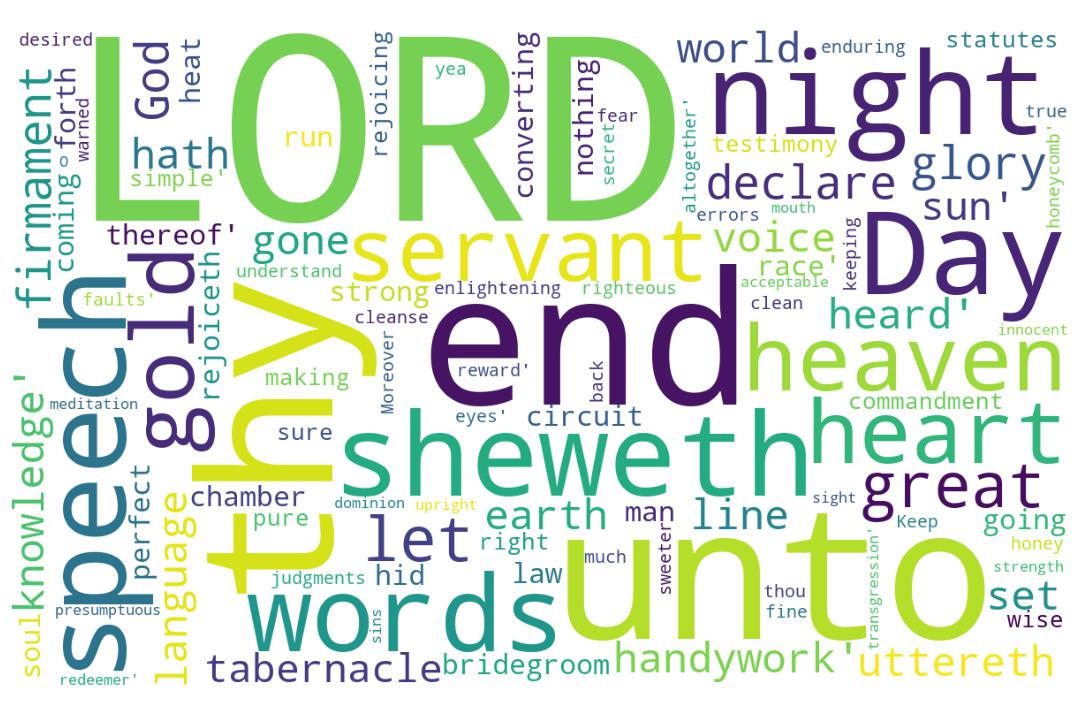
\includegraphics[width=\linewidth]{19OT-Psalms/Psalm19-WordCloud.jpg}
  \caption{Psalm 19 Word Cloud}
  \label{fig:Psalm 19 word Cloud}
\end{figure}

\marginpar{\scriptsize \centering \fcolorbox{bone}{lime}{\textbf{PROFITTING FROM REVELATION}}\\ Psalm 19:1-14) \begin{compactenum}[I.][8]
    \item \textbf{Revealing} \index[scripture]{Psalms!Psa 019:02}(Psa 19:2)
    \item \textbf{Redeeming} \index[scripture]{Psalms!Psa 019:07}(Psa 19:7)
    \item \textbf{Rejoicing} \index[scripture]{Psalms!Psa 019:08}(Psa 19:8)
    \item \textbf{Refreshing} \index[scripture]{Psalms!Psa 019:10}(Psa 19:10) (Sweet)
    \item \textbf{Rewarding} \index[scripture]{Psalms!Psa 019:11}(Psa 19:11)
    \item \textbf{Readying} \index[scripture]{Psalms!Psa 019:11}(Psa 19:11)
    \item \textbf{Refining} \index[scripture]{Psalms!Psa 019:12}(Psa 19:12)
\end{compactenum}}

\marginpar{\scriptsize \centering \fcolorbox{bone}{yellow}{\textbf{REVEALED TRUTH IS}}\\ Psalm 19:1-14) \begin{compactenum}[I.][8]
    \item \textbf{Communicated} \index[scripture]{Psalms!Psa 019:01}(Psa 19:1)
    \item \textbf{Continuous} \index[scripture]{Psalms!Psa 019:02}(Psa 19:2)
    \item \textbf{Indicative} \index[scripture]{Psalms!Psa 019:05}(Psa 19:5)
    \item \textbf{Climactic} \index[scripture]{Psalms!Psa 019:06}(Psa 19:6)
    \item \textbf{Converting} \index[scripture]{Psalms!Psa 019:07}(Psa 19:7)
    \item To be \textbf{Coveted} \index[scripture]{Psalms!Psa 019:10}(Psa 19:10)
    \item \textbf{Corrective} \index[scripture]{Psalms!Psa 019:11}(Psa 19:11)
\end{compactenum}}

\marginpar{\scriptsize \centering \fcolorbox{bone}{black}{\textbf{\textcolor[cmyk]{0,0,0,0}{WHAT HEAVENS DECLARE}}}\\ (Psalm 19:1-14)  
\begin{compactenum}[I.][8]
    \item \textbf{Reality}  -- hard to ignore!
    \item \textbf{Revelation} \index[scripture]{Psalms!Psa 019:01}(Psa 19:1)
    \item \textbf{A Return} \index[scripture]{Psalms!Psa 019:05}(Psa 19:5) -- bridegroom coming
    \item \textbf{A Requirement} \index[scripture]{Psalms!Psa 019:07-14}(Psa 19:7-14)
    \item \textbf{Rejoicing in God} \index[scripture]{Psalms!Psa 019:08}(Psa 19:8)
    \item \textbf{Righteousness} \index[scripture]{Psalms!Psa 019:09}(Psa 19:9)
    \item \textbf{A Reward for Obedience} \index[scripture]{Psalms!Psa 019:11}(Psa 19:11)
\end{compactenum}}

\marginpar{\scriptsize \centering \fcolorbox{bone}{blue}{\textbf{\textcolor[cmyk]{0,0,0,0}{REVELATION}}}\\ (Psalm 19:1-14)  
\begin{compactenum}[I.][8]
\item A Witness (Psa 19:3) 
\item Words (Psa 19:4)
\item Wisdom (Psa 19:7) 
\item A Warning (Psa 19:11)
\item Wonder
\end{compactenum}}

\footnote{\textcolor[cmyk]{0.99998,1,0,0}{\hyperlink{TOC}{Return to end of Table of Contents.}}}\footnote{\href{https://www.audioverse.org/english/audiobibles/books/ENGKJV/O/Ps/1}{\textcolor[cmyk]{0.99998,1,0,0}{Psalms Audio}}}\textcolor[cmyk]{0.99998,1,0,0}{To the chief Musician, A Psalm of David.}\\
\\
\textcolor[cmyk]{0.99998,1,0,0}{The heavens \fcolorbox{bone}{yellow}{declare} the glory of God; and the firmament sheweth his handywork.}\footnote{\textbf{Genesis 1:6-7} - And God said, Let there be a firmament in the midst of the waters, and let it divide the waters from the waters. [7] And God made the firmament, and divided the waters which were under the firmament from the waters which were above the firmament: and it was so. 8 And God called the firmament Heaven. And the evening and the morning were the second day.}
[2] \textcolor[cmyk]{0.99998,1,0,0}{\fcolorbox{bone}{yellow}{Day unto day} uttereth speech, and night unto night \fcolorbox{bone}{lime}{sheweth} \fcolorbox{bone}{lime}{knowledge}.}
[3] \textcolor[cmyk]{0.99998,1,0,0}{\emph{There} \emph{is} no speech nor language, \emph{where} their voice is not heard.}
[4] \textcolor[cmyk]{0.99998,1,0,0}{Their line is gone out through all the earth, and their words to the end of the world. In them hath he set a tabernacle for the sun,}
[5] \textcolor[cmyk]{0.99998,1,0,0}{Which \emph{is} \fcolorbox{bone}{yellow}{as a bridegroom} coming out of his chamber, \emph{and} rejoiceth as a strong man to run a race.}\footnote{\textbf{Joel 2:16} -  Gather the people, sanctify the congregation, assemble the elders, gather the children, and those that suck the breasts: let the bridegroom go forth of his chamber, and the bride out of her closet.}
[6] \textcolor[cmyk]{0.99998,1,0,0}{His going forth \emph{is} from the end of the heaven, and his circuit \fcolorbox{bone}{yellow}{unto the ends of it}: and there is nothing hid from the heat thereof.}
[7] \textcolor[cmyk]{0.99998,1,0,0}{The law of the LORD \emph{is} perfect, \fcolorbox{bone}{lime}{converting} the soul: the testimony of the LORD \emph{is} sure, making wise the simple.}
[8] \textcolor[cmyk]{0.99998,1,0,0}{The statutes of the LORD \emph{are} right, \fcolorbox{bone}{lime}{rejoicing} the heart: the commandment of the LORD \emph{is} pure, enlightening the eyes.}\footnote{\textbf{Ephesian 1:18} - The eyes of your understanding being enlightened; that ye may know what is the hope of his calling, and what the riches of the glory of his inheritance in the saints,}
[9] \textcolor[cmyk]{0.99998,1,0,0}{The fear of the LORD \emph{is} clean, enduring for ever: the judgments of the LORD \emph{are} true \emph{and} righteous altogether.}
[10] \textcolor[cmyk]{0.99998,1,0,0}{More \fcolorbox{bone}{yellow}{to be desired} \emph{are} \emph{they} than gold, yea, than much fine gold: \fcolorbox{bone}{lime}{sweeter} also than honey and the honeycomb.}
[11] \textcolor[cmyk]{0.99998,1,0,0}{Moreover by them is thy servant \fcolorbox{bone}{lime}{warned}: \emph{and} in keeping of them \emph{there} \emph{is} great \fcolorbox{bone}{lime}{reward}.}
[12] \textcolor[cmyk]{0.99998,1,0,0}{Who can understand \emph{his} errors? \fcolorbox{bone}{lime}{cleanse} thou me from secret \emph{faults}.}\footnote{\textbf{Jeremiah 17:9} - The heart is deceitful above all things, and desperately wicked: who can know it?}
[13] \textcolor[cmyk]{0.99998,1,0,0}{Keep back thy servant also from presumptuous \emph{sins}; let them not have dominion over me: then shall I be upright, and I shall be innocent from the great \fcolorbox{bone}{MYGOLD}{transgression}.}\marginpar{\scriptsize \textcolor[rgb]{0.00,0.545,0.269}{$\rightarrow$Described(1) law of the Lord (vs 7) (2) testimony of the Lord)  (vs 7) , (3) statutes of the Lord  (vs 8) , (4) commandment of the Lord  (vs 8) , (5) fear of the Lord  (vs 9) , and (6) judgments of the Lord (vs 9).}}
[14] \textcolor[cmyk]{0.99998,1,0,0}{Let the words of my mouth, and the meditation of my heart, be acceptable in thy sight, O LORD, my strength, and my redeemer.}
%\marginpar{\textcolor[rgb]{0.13, 0.55, 0.13}{\tiny What Creation Provides: \begin{compactenum}[I.][7]
%\end{compactenum} } } 


\section{Psalm 19 Comments}

\subsection{Numeric Nuggets}
\textbf{13:} Verse 1 has 13 words.  The 13-letter word ``trangression'' shows up in verse 13.

\subsection{Psalm 19 Introduction}

Seven items are listed in Psalm 19, as a logical follow-on to the revelation in the early part of the psalm (identified by the phrase ``of the Lord'', found in verses 7, 8, and 9, each at words number 3 and 13). These are the things that are doing the speaking in the psalm. But we must add one more, the heavens:\\
\begin{compactenum}
	\item The \textbf{heavens}  (verse 1)
	\item The \textbf{law} of the Lord (verse 7)
	\item The \textbf{testimony} of the Lord (verse 7)
	\item The \textbf{statutes} of the Lord (verse 8)
	\item The \textbf{commandments} of the Lord (verse 8)
	\item The \textbf{fear} of the Lord (verse 9)
	\item The \textbf{judgments} of the Lord (verse 9)	\\
\end{compactenum}
\noindent These point also to Psalm 119, where they are discussed in depth.

\subsection{Numeric Nuggets}
There are thirteen words in Psalm 19:1, suggesting in general, that mankind will rebel against the general revelation of creation. The thirteen-letter word ``transgression'' is used in Psalm 19, notably in verse 13. 

\subsection{Psalm 19:1}
This verse is corrupted in new translations (see Table~\ref{table:CorruptionPsalm-19-1}).

\begin{center}

\begin{table}[ht]
\centering
\begin{tabular}{|p{.5in}|p{3.5in}|}
\hline

\textcolor[rgb]{0.00,0.00,1.00}{AV} & \textcolor[rgb]{0.00,0.00,1.00}{The heavens declare the glory of God; and the \fcolorbox{black}{lime}{firmament} sheweth his handywork.} \\ \hline \hline

ASV &  The heavens declare the glory of God; And the firmament showeth his handiwork. \\ \hline
%
CEB &  Heaven is declaring God’s glory;  he sky is proclaiming his handiwork.\\ \hline
%
ESV & The heavens declare the glory of God, and the sky above proclaims his handiwork. \\ \hline
%
NASV &  The heavens are telling of the glory of God; And their expanse is declaring the work of His hands. \\ \hline
%
MEV & The heavens declare the glory of God,  and the firmament shows His handiwork.\\ \hline
%
NIV &  The heavens declare the glory of God; the skies proclaim the work of his hands. \\ \hline
%
NKJV &  The heavens declare the glory of God; And the firmament shows His handiwork.\\ \hline
%
RSV &  The heavens are telling the glory of God; and the firmament proclaims his handiwork.\\ \hline \hline

\multicolumn{2}{|p{4.2in}|}{{\textcolor{jungle}{Some modern translations, change the word ``firmament'' with ``sky'' or ``expanse'', removing the reference to a part of the creation in Genesis 1:6, and to the structure of the universe.}}} \\ \hline

\end{tabular}
\caption[Corruption Alert: Psalm 19:1]{Corruption Alert: Psalm 19:1} \label{table:CorruptionPsalm-19-1}
\end{table}

\end{center}





%%%%%%%%%%%%%%%%%%%



\subsection{Psalm 19:12}
The immediate cross-reference that comes to mind is Jeremiah 17:9,10.\footnote{\textbf{Jeremiah 17:9, 10} - The heart is deceitful above all things, and desperately wicked: who can know it? [10] I the LORD search the heart, I try the reins, even to give every man according to his ways, and according to the fruit of his doings.} This, though, is just one of the 44 references to the ``who can'' (both cases) phrase in scripture.

\include{WordsAndPhrasesInScripture/WAPFIS-whoCan}

\subsection{Psalm 19:13}
This verse is corrupted in new translations (see Table~\ref{table:CorruptionPsalm-19-13}).
%%%%%%%%%%%%%%%%%%%%%%%%%%%%%%%%%%%%%%%%%%%%%%%%

\begin{center}

\begin{table}[ht]
\centering
\begin{tabular}{|p{.5in}|p{3.5in}|}
\hline

\textcolor[rgb]{0.00,0.00,1.00}{AV} & \textcolor[rgb]{0.00,0.00,1.00}{Keep back thy servant also from presumptuous sins; let them not have dominion over me: then shall I be upright, and I shall be innocent from  \fcolorbox{black}{lime}{the} great transgression.} \\ \hline \hline

ASV &  Keep back thy servant also from presumptuous sins; Let them not have dominion over me: Then shall I be upright, And I shall be clear from great transgression. \\ \hline
%
CEB &  and save your servant from willful sins.  Don’t let them rule me. Then I’ll be completely blameless;  I’ll be innocent of great wrongdoing.\\ \hline
%
ESV & Keep back your servant also from presumptuous sins;   let them not have dominion over me! Then I shall be blameless,   and innocent of great transgression. \\ \hline
%
NASV &  Also keep back Your servant from presumptuous sins; Let them not rule over me; Then I will be blameless, And I shall be acquitted of great transgression. \\ \hline
%
MEV & Keep back Your servant also from presumptuous sins;   may they not rule over me. Then I will be upright   and innocent from great transgression.\\ \hline
%
NIV &  Keep your servant also from willful sins;  may they not rule over me. Then I will be blameless,  innocent of great transgression. \\ \hline
%
NKJV &  Keep back Your servant also from presumptuous sins; Let them not have dominion over me. Then I shall be blameless, And I shall be innocent of [a]great transgression. \\ \hline
%
RSV &  Keep back thy servant also from presumptuous sins;  let them not have dominion over me! Then I shall be blameless,  and innocent of great transgression.\\ \hline \hline

\multicolumn{2}{|p{4.2in}|}{{\textcolor{jungle}{Modern translations remove the definite article ``the'' which modifies ``great transgression'', thus destroying its clear definition. It it what is committed in John 19:15 and Matthew 12:31-32. The sin, the unforgivable sin, is that of rejecting the Lord Jesus Christ.}}} \\ \hline

\end{tabular}
\caption[Corruption Alert: Psalm 19:13]{Corruption Alert: Psalm 19:13} \label{table:CorruptionPsalm-19-13}
\end{table}

\end{center}

%%%%%%%%%%%%%%%%%%%%%%%%%%%%%%%%%%%%%%%%%%%%%%%%


%\index[NWIV]{13!Psalms!Psa 19:1}\index[AWIP]{The!Psalms!Psa 19:1}\index[AWIP]{heavens!Psalms!Psa 19:1}\index[AWIP]{declare!Psalms!Psa 19:1}\index[AWIP]{the!Psalms!Psa 19:1}\index[AWIP]{the!Psalms!Psa 19:1 (2)}\index[AWIP]{glory!Psalms!Psa 19:1}\index[AWIP]{of!Psalms!Psa 19:1}\index[AWIP]{God!Psalms!Psa 19:1}\index[AWIP]{and!Psalms!Psa 19:1}\index[AWIP]{firmament!Psalms!Psa 19:1}\index[AWIP]{sheweth!Psalms!Psa 19:1}\index[AWIP]{his!Psalms!Psa 19:1}\index[AWIP]{handywork!Psalms!Psa 19:1}

\index[NWIV]{11!Psalms!Psa 19:2}\index[AWIP]{Day!Psalms!Psa 19:2}\index[AWIP]{unto!Psalms!Psa 19:2}\index[AWIP]{unto!Psalms!Psa 19:2 (2)}\index[AWIP]{day!Psalms!Psa 19:2}\index[AWIP]{uttereth!Psalms!Psa 19:2}\index[AWIP]{speech!Psalms!Psa 19:2}\index[AWIP]{and!Psalms!Psa 19:2}\index[AWIP]{night!Psalms!Psa 19:2}\index[AWIP]{night!Psalms!Psa 19:2 (2)}\index[AWIP]{sheweth!Psalms!Psa 19:2}\index[AWIP]{knowledge!Psalms!Psa 19:2}

\index[NWIV]{12!Psalms!Psa 19:3}\index[AWIP]{\emph{There}!Psalms!Psa 19:3}\index[AWIP]{\emph{is}!Psalms!Psa 19:3}\index[AWIP]{no!Psalms!Psa 19:3}\index[AWIP]{speech!Psalms!Psa 19:3}\index[AWIP]{nor!Psalms!Psa 19:3}\index[AWIP]{language!Psalms!Psa 19:3}\index[AWIP]{\emph{where}!Psalms!Psa 19:3}\index[AWIP]{their!Psalms!Psa 19:3}\index[AWIP]{voice!Psalms!Psa 19:3}\index[AWIP]{is!Psalms!Psa 19:3}\index[AWIP]{not!Psalms!Psa 19:3}\index[AWIP]{heard!Psalms!Psa 19:3}\index[AWIP]{\emph{There}!Psalms!Psa 19:3}\index[AWIP]{\emph{is}!Psalms!Psa 19:3}\index[AWIP]{\emph{where}!Psalms!Psa 19:3}

\index[NWIV]{28!Psalms!Psa 19:4}\index[AWIP]{Their!Psalms!Psa 19:4}\index[AWIP]{line!Psalms!Psa 19:4}\index[AWIP]{is!Psalms!Psa 19:4}\index[AWIP]{gone!Psalms!Psa 19:4}\index[AWIP]{out!Psalms!Psa 19:4}\index[AWIP]{through!Psalms!Psa 19:4}\index[AWIP]{all!Psalms!Psa 19:4}\index[AWIP]{the!Psalms!Psa 19:4}\index[AWIP]{the!Psalms!Psa 19:4 (2)}\index[AWIP]{the!Psalms!Psa 19:4 (3)}\index[AWIP]{the!Psalms!Psa 19:4 (4)}\index[AWIP]{earth!Psalms!Psa 19:4}\index[AWIP]{and!Psalms!Psa 19:4}\index[AWIP]{their!Psalms!Psa 19:4}\index[AWIP]{words!Psalms!Psa 19:4}\index[AWIP]{to!Psalms!Psa 19:4}\index[AWIP]{end!Psalms!Psa 19:4}\index[AWIP]{of!Psalms!Psa 19:4}\index[AWIP]{world!Psalms!Psa 19:4}\index[AWIP]{In!Psalms!Psa 19:4}\index[AWIP]{them!Psalms!Psa 19:4}\index[AWIP]{hath!Psalms!Psa 19:4}\index[AWIP]{he!Psalms!Psa 19:4}\index[AWIP]{set!Psalms!Psa 19:4}\index[AWIP]{a!Psalms!Psa 19:4}\index[AWIP]{tabernacle!Psalms!Psa 19:4}\index[AWIP]{for!Psalms!Psa 19:4}\index[AWIP]{sun!Psalms!Psa 19:4}

\index[NWIV]{20!Psalms!Psa 19:5}\index[AWIP]{Which!Psalms!Psa 19:5}\index[AWIP]{\emph{is}!Psalms!Psa 19:5}\index[AWIP]{as!Psalms!Psa 19:5}\index[AWIP]{as!Psalms!Psa 19:5 (2)}\index[AWIP]{a!Psalms!Psa 19:5}\index[AWIP]{a!Psalms!Psa 19:5 (2)}\index[AWIP]{a!Psalms!Psa 19:5 (3)}\index[AWIP]{bridegroom!Psalms!Psa 19:5}\index[AWIP]{coming!Psalms!Psa 19:5}\index[AWIP]{out!Psalms!Psa 19:5}\index[AWIP]{of!Psalms!Psa 19:5}\index[AWIP]{his!Psalms!Psa 19:5}\index[AWIP]{chamber!Psalms!Psa 19:5}\index[AWIP]{\emph{and}!Psalms!Psa 19:5}\index[AWIP]{rejoiceth!Psalms!Psa 19:5}\index[AWIP]{strong!Psalms!Psa 19:5}\index[AWIP]{man!Psalms!Psa 19:5}\index[AWIP]{to!Psalms!Psa 19:5}\index[AWIP]{run!Psalms!Psa 19:5}\index[AWIP]{race!Psalms!Psa 19:5}\index[AWIP]{\emph{is}!Psalms!Psa 19:5}\index[AWIP]{\emph{and}!Psalms!Psa 19:5}

\index[NWIV]{27!Psalms!Psa 19:6}\index[AWIP]{His!Psalms!Psa 19:6}\index[AWIP]{going!Psalms!Psa 19:6}\index[AWIP]{forth!Psalms!Psa 19:6}\index[AWIP]{\emph{is}!Psalms!Psa 19:6}\index[AWIP]{from!Psalms!Psa 19:6}\index[AWIP]{from!Psalms!Psa 19:6 (2)}\index[AWIP]{the!Psalms!Psa 19:6}\index[AWIP]{the!Psalms!Psa 19:6 (2)}\index[AWIP]{the!Psalms!Psa 19:6 (3)}\index[AWIP]{the!Psalms!Psa 19:6 (4)}\index[AWIP]{end!Psalms!Psa 19:6}\index[AWIP]{of!Psalms!Psa 19:6}\index[AWIP]{of!Psalms!Psa 19:6 (2)}\index[AWIP]{heaven!Psalms!Psa 19:6}\index[AWIP]{and!Psalms!Psa 19:6}\index[AWIP]{and!Psalms!Psa 19:6 (2)}\index[AWIP]{his!Psalms!Psa 19:6}\index[AWIP]{circuit!Psalms!Psa 19:6}\index[AWIP]{unto!Psalms!Psa 19:6}\index[AWIP]{ends!Psalms!Psa 19:6}\index[AWIP]{it!Psalms!Psa 19:6}\index[AWIP]{there!Psalms!Psa 19:6}\index[AWIP]{is!Psalms!Psa 19:6}\index[AWIP]{nothing!Psalms!Psa 19:6}\index[AWIP]{hid!Psalms!Psa 19:6}\index[AWIP]{heat!Psalms!Psa 19:6}\index[AWIP]{thereof!Psalms!Psa 19:6}\index[AWIP]{\emph{is}!Psalms!Psa 19:6}

\index[NWIV]{21!Psalms!Psa 19:7}\index[AWIP]{The!Psalms!Psa 19:7}\index[AWIP]{law!Psalms!Psa 19:7}\index[AWIP]{of!Psalms!Psa 19:7}\index[AWIP]{of!Psalms!Psa 19:7 (2)}\index[AWIP]{the!Psalms!Psa 19:7}\index[AWIP]{the!Psalms!Psa 19:7 (2)}\index[AWIP]{the!Psalms!Psa 19:7 (3)}\index[AWIP]{the!Psalms!Psa 19:7 (4)}\index[AWIP]{the!Psalms!Psa 19:7 (5)}\index[AWIP]{LORD!Psalms!Psa 19:7}\index[AWIP]{LORD!Psalms!Psa 19:7 (2)}\index[AWIP]{\emph{is}!Psalms!Psa 19:7}\index[AWIP]{\emph{is}!Psalms!Psa 19:7 (2)}\index[AWIP]{perfect!Psalms!Psa 19:7}\index[AWIP]{converting!Psalms!Psa 19:7}\index[AWIP]{soul!Psalms!Psa 19:7}\index[AWIP]{testimony!Psalms!Psa 19:7}\index[AWIP]{sure!Psalms!Psa 19:7}\index[AWIP]{making!Psalms!Psa 19:7}\index[AWIP]{wise!Psalms!Psa 19:7}\index[AWIP]{simple!Psalms!Psa 19:7}\index[AWIP]{\emph{is}!Psalms!Psa 19:7}\index[AWIP]{\emph{is}!Psalms!Psa 19:7 (2)}

\index[NWIV]{20!Psalms!Psa 19:8}\index[AWIP]{The!Psalms!Psa 19:8}\index[AWIP]{statutes!Psalms!Psa 19:8}\index[AWIP]{of!Psalms!Psa 19:8}\index[AWIP]{of!Psalms!Psa 19:8 (2)}\index[AWIP]{the!Psalms!Psa 19:8}\index[AWIP]{the!Psalms!Psa 19:8 (2)}\index[AWIP]{the!Psalms!Psa 19:8 (3)}\index[AWIP]{the!Psalms!Psa 19:8 (4)}\index[AWIP]{the!Psalms!Psa 19:8 (5)}\index[AWIP]{LORD!Psalms!Psa 19:8}\index[AWIP]{LORD!Psalms!Psa 19:8 (2)}\index[AWIP]{\emph{are}!Psalms!Psa 19:8}\index[AWIP]{right!Psalms!Psa 19:8}\index[AWIP]{rejoicing!Psalms!Psa 19:8}\index[AWIP]{heart!Psalms!Psa 19:8}\index[AWIP]{commandment!Psalms!Psa 19:8}\index[AWIP]{\emph{is}!Psalms!Psa 19:8}\index[AWIP]{pure!Psalms!Psa 19:8}\index[AWIP]{enlightening!Psalms!Psa 19:8}\index[AWIP]{eyes!Psalms!Psa 19:8}\index[AWIP]{\emph{are}!Psalms!Psa 19:8}\index[AWIP]{\emph{is}!Psalms!Psa 19:8}

\index[NWIV]{20!Psalms!Psa 19:9}\index[AWIP]{The!Psalms!Psa 19:9}\index[AWIP]{fear!Psalms!Psa 19:9}\index[AWIP]{of!Psalms!Psa 19:9}\index[AWIP]{of!Psalms!Psa 19:9 (2)}\index[AWIP]{the!Psalms!Psa 19:9}\index[AWIP]{the!Psalms!Psa 19:9 (2)}\index[AWIP]{the!Psalms!Psa 19:9 (3)}\index[AWIP]{LORD!Psalms!Psa 19:9}\index[AWIP]{LORD!Psalms!Psa 19:9 (2)}\index[AWIP]{\emph{is}!Psalms!Psa 19:9}\index[AWIP]{clean!Psalms!Psa 19:9}\index[AWIP]{enduring!Psalms!Psa 19:9}\index[AWIP]{for!Psalms!Psa 19:9}\index[AWIP]{ever!Psalms!Psa 19:9}\index[AWIP]{judgments!Psalms!Psa 19:9}\index[AWIP]{\emph{are}!Psalms!Psa 19:9}\index[AWIP]{true!Psalms!Psa 19:9}\index[AWIP]{\emph{and}!Psalms!Psa 19:9}\index[AWIP]{righteous!Psalms!Psa 19:9}\index[AWIP]{altogether!Psalms!Psa 19:9}\index[AWIP]{\emph{is}!Psalms!Psa 19:9}\index[AWIP]{\emph{are}!Psalms!Psa 19:9}\index[AWIP]{\emph{and}!Psalms!Psa 19:9}

\index[NWIV]{20!Psalms!Psa 19:10}\index[AWIP]{More!Psalms!Psa 19:10}\index[AWIP]{to!Psalms!Psa 19:10}\index[AWIP]{be!Psalms!Psa 19:10}\index[AWIP]{desired!Psalms!Psa 19:10}\index[AWIP]{\emph{are}!Psalms!Psa 19:10}\index[AWIP]{\emph{they}!Psalms!Psa 19:10}\index[AWIP]{than!Psalms!Psa 19:10}\index[AWIP]{than!Psalms!Psa 19:10 (2)}\index[AWIP]{than!Psalms!Psa 19:10 (3)}\index[AWIP]{gold!Psalms!Psa 19:10}\index[AWIP]{gold!Psalms!Psa 19:10 (2)}\index[AWIP]{yea!Psalms!Psa 19:10}\index[AWIP]{much!Psalms!Psa 19:10}\index[AWIP]{fine!Psalms!Psa 19:10}\index[AWIP]{sweeter!Psalms!Psa 19:10}\index[AWIP]{also!Psalms!Psa 19:10}\index[AWIP]{honey!Psalms!Psa 19:10}\index[AWIP]{and!Psalms!Psa 19:10}\index[AWIP]{the!Psalms!Psa 19:10}\index[AWIP]{honeycomb!Psalms!Psa 19:10}\index[AWIP]{\emph{are}!Psalms!Psa 19:10}\index[AWIP]{\emph{they}!Psalms!Psa 19:10}

\index[NWIV]{16!Psalms!Psa 19:11}\index[AWIP]{Moreover!Psalms!Psa 19:11}\index[AWIP]{by!Psalms!Psa 19:11}\index[AWIP]{them!Psalms!Psa 19:11}\index[AWIP]{them!Psalms!Psa 19:11 (2)}\index[AWIP]{is!Psalms!Psa 19:11}\index[AWIP]{thy!Psalms!Psa 19:11}\index[AWIP]{servant!Psalms!Psa 19:11}\index[AWIP]{warned!Psalms!Psa 19:11}\index[AWIP]{\emph{and}!Psalms!Psa 19:11}\index[AWIP]{in!Psalms!Psa 19:11}\index[AWIP]{keeping!Psalms!Psa 19:11}\index[AWIP]{of!Psalms!Psa 19:11}\index[AWIP]{\emph{there}!Psalms!Psa 19:11}\index[AWIP]{\emph{is}!Psalms!Psa 19:11}\index[AWIP]{great!Psalms!Psa 19:11}\index[AWIP]{reward!Psalms!Psa 19:11}\index[AWIP]{\emph{and}!Psalms!Psa 19:11}\index[AWIP]{\emph{there}!Psalms!Psa 19:11}\index[AWIP]{\emph{is}!Psalms!Psa 19:11}

\index[NWIV]{11!Psalms!Psa 19:12}\index[AWIP]{Who!Psalms!Psa 19:12}\index[AWIP]{can!Psalms!Psa 19:12}\index[AWIP]{understand!Psalms!Psa 19:12}\index[AWIP]{\emph{his}!Psalms!Psa 19:12}\index[AWIP]{errors?!Psalms!Psa 19:12}\index[AWIP]{cleanse!Psalms!Psa 19:12}\index[AWIP]{thou!Psalms!Psa 19:12}\index[AWIP]{me!Psalms!Psa 19:12}\index[AWIP]{from!Psalms!Psa 19:12}\index[AWIP]{secret!Psalms!Psa 19:12}\index[AWIP]{\emph{faults}!Psalms!Psa 19:12}\index[AWIP]{\emph{his}!Psalms!Psa 19:12}\index[AWIP]{\emph{faults}!Psalms!Psa 19:12}

\index[NWIV]{29!Psalms!Psa 19:13}\index[AWIP]{Keep!Psalms!Psa 19:13}\index[AWIP]{back!Psalms!Psa 19:13}\index[AWIP]{thy!Psalms!Psa 19:13}\index[AWIP]{servant!Psalms!Psa 19:13}\index[AWIP]{also!Psalms!Psa 19:13}\index[AWIP]{from!Psalms!Psa 19:13}\index[AWIP]{from!Psalms!Psa 19:13 (2)}\index[AWIP]{presumptuous!Psalms!Psa 19:13}\index[AWIP]{\emph{sins}!Psalms!Psa 19:13}\index[AWIP]{let!Psalms!Psa 19:13}\index[AWIP]{them!Psalms!Psa 19:13}\index[AWIP]{not!Psalms!Psa 19:13}\index[AWIP]{have!Psalms!Psa 19:13}\index[AWIP]{dominion!Psalms!Psa 19:13}\index[AWIP]{over!Psalms!Psa 19:13}\index[AWIP]{me!Psalms!Psa 19:13}\index[AWIP]{then!Psalms!Psa 19:13}\index[AWIP]{shall!Psalms!Psa 19:13}\index[AWIP]{shall!Psalms!Psa 19:13 (2)}\index[AWIP]{I!Psalms!Psa 19:13}\index[AWIP]{I!Psalms!Psa 19:13 (2)}\index[AWIP]{be!Psalms!Psa 19:13}\index[AWIP]{be!Psalms!Psa 19:13 (2)}\index[AWIP]{upright!Psalms!Psa 19:13}\index[AWIP]{and!Psalms!Psa 19:13}\index[AWIP]{innocent!Psalms!Psa 19:13}\index[AWIP]{the!Psalms!Psa 19:13}\index[AWIP]{great!Psalms!Psa 19:13}\index[AWIP]{transgression!Psalms!Psa 19:13}\index[AWIP]{\emph{sins}!Psalms!Psa 19:13}

\index[NWIV]{24!Psalms!Psa 19:14}\index[AWIP]{Let!Psalms!Psa 19:14}\index[AWIP]{the!Psalms!Psa 19:14}\index[AWIP]{the!Psalms!Psa 19:14 (2)}\index[AWIP]{words!Psalms!Psa 19:14}\index[AWIP]{of!Psalms!Psa 19:14}\index[AWIP]{of!Psalms!Psa 19:14 (2)}\index[AWIP]{my!Psalms!Psa 19:14}\index[AWIP]{my!Psalms!Psa 19:14 (2)}\index[AWIP]{my!Psalms!Psa 19:14 (3)}\index[AWIP]{my!Psalms!Psa 19:14 (4)}\index[AWIP]{mouth!Psalms!Psa 19:14}\index[AWIP]{and!Psalms!Psa 19:14}\index[AWIP]{and!Psalms!Psa 19:14 (2)}\index[AWIP]{meditation!Psalms!Psa 19:14}\index[AWIP]{heart!Psalms!Psa 19:14}\index[AWIP]{be!Psalms!Psa 19:14}\index[AWIP]{acceptable!Psalms!Psa 19:14}\index[AWIP]{in!Psalms!Psa 19:14}\index[AWIP]{thy!Psalms!Psa 19:14}\index[AWIP]{sight!Psalms!Psa 19:14}\index[AWIP]{O!Psalms!Psa 19:14}\index[AWIP]{LORD!Psalms!Psa 19:14}\index[AWIP]{strength!Psalms!Psa 19:14}\index[AWIP]{redeemer!Psalms!Psa 19:14}


\section{Psalm 19 Outlines}

\subsection{My Outlines}

\subsubsection{Profiting from God's Revelation}
\index[speaker]{Keith Anthony!Psalm 019 (Profiting from God's Revelation)}
\index[series]{Psalms (Keith Anthony)!Psalm 019 (Profiting from God's Revelation)}
\index[date]{2017/01/19!Psalm 019 (Profiting from God's Revelation) (Keith Anthony)}
\begin{compactenum}[I.]
    \item \textbf{Revealing} \index[scripture]{Psalms!Psa 019:02}(Psa 19:2)
    \item \textbf{Redeeming} \index[scripture]{Psalms!Psa 019:07}(Psa 19:7)
    \item \textbf{Rejoicing} \index[scripture]{Psalms!Psa 019:08}(Psa 19:8)
    \item \textbf{Refreshing} \index[scripture]{Psalms!Psa 019:10}(Psa 19:10) (Sweet)
    \item \textbf{Rewarding} \index[scripture]{Psalms!Psa 019:11}(Psa 19:11)
    \item \textbf{Readying} \index[scripture]{Psalms!Psa 019:11}(Psa 19:11)
    \item \textbf{Refining} \index[scripture]{Psalms!Psa 019:12}(Psa 19:12)
\end{compactenum}
\subsubsection{God's Revealed Truth Is}
\index[speaker]{Keith Anthony!Psalm 019 (God's Revealed Truth Is)}
\index[series]{Psalms (Keith Anthony)!Psalm 019 (God's Revealed Truth Is)}
\index[date]{2016/06/25!Psalm 019 (God's Revealed Truth Is) (Keith Anthony)}
\begin{compactenum}[I.]
    \item \textbf{Communicated} \index[scripture]{Psalms!Psa 019:01}(Psa 19:1)
    \item \textbf{Continuous} \index[scripture]{Psalms!Psa 019:02}(Psa 19:2)
    \item \textbf{Indicative} \index[scripture]{Psalms!Psa 019:05}(Psa 19:5)
    \item \textbf{Climactic} \index[scripture]{Psalms!Psa 019:06}(Psa 19:6)
    \item \textbf{Converting} \index[scripture]{Psalms!Psa 019:07}(Psa 19:7)
    \item To be \textbf{Coveted} \index[scripture]{Psalms!Psa 019:10}(Psa 19:10)
    \item \textbf{Corrective} \index[scripture]{Psalms!Psa 019:11}(Psa 19:11)
\end{compactenum}

\subsubsection{What the Heavens Declare}
\index[speaker]{Keith Anthony!Psalm 019 (What the Heavens Declare)}
\index[series]{Psalms (Keith Anthony)!Psalm 019 (What the Heavens Declare)}
\index[date]{unknown!Psalm 019 (What the Heavens Declare) (Keith Anthony)}
\begin{compactenum}[I.]
    \item \textbf{Reality}  -- hard to ignore!
    \item \textbf{Revelation} \index[scripture]{Psalms!Psa 019:01}(Psa 19:1)
    \item \textbf{A Return} \index[scripture]{Psalms!Psa 019:05}(Psa 19:5) -- bridegroom coming
    \item \textbf{A Requirement} \index[scripture]{Psalms!Psa 019:07-14}(Psa 19:7-14)
    \item \textbf{Rejoicing in God} \index[scripture]{Psalms!Psa 019:08}(Psa 19:8)
    \item \textbf{Righteousness} \index[scripture]{Psalms!Psa 019:09}(Psa 19:9)
    \item \textbf{A Reward for Obedience} \index[scripture]{Psalms!Psa 019:11}(Psa 19:11)
\end{compactenum}

\subsubsection{Revelation}
\index[speaker]{Keith Anthony!Psalm 019 (Revelation)}
\index[series]{Psalms (Keith Anthony)!Psalm 019 (Revelation)}
\index[date]{2017/06/24!Psalm 019 (Revelation) (Keith Anthony)}
\begin{compactenum}[I.]
\item \textbf{Unusual} %\index[scripture]{Psalms!Psa 019:01}(Psalm 19:1)
\item \textbf{Unceasing} \index[scripture]{Psalms!Psa 019:02}(Psa 19:2)
\item \textbf{Universal} \index[scripture]{Psalms!Psa 019:03}(Psa 19:3)
\item \textbf{Un-escapable} %\index[scripture]{Psalms!Psa 019:01}(Psalm 19:1)
\item \textbf{Unavoidable} %\index[scripture]{Psalms!Psa 019:01}(Psalm 19:1)
\item \textbf{Unmistakeable} %\index[scripture]{Psalms!Psa 019:01}(Psalm 19:1)
\item \textbf{Unexplainable} %\index[scripture]{Psalms!Psa 019:01}(Psalm 19:1)
\end{compactenum}

\subsubsection{What Creation Provides}
\index[speaker]{Keith Anthony!Psalm 019 (What Creation Provides)}
\index[series]{Psalms (Keith Anthony)!Psalm 019 (What Creation Provides)}
\index[date]{2017/06/24!Psalm 019 (What Creation Provides) (Keith Anthony)}
\begin{compactenum}[I.]
\item \textbf{Wonder} \index[scripture]{Psalms!Psa 019:01}(Psa 19:1)
\item A \textbf{Witness} \index[scripture]{Psalms!Psa 019:03}(Psa 19:3) 
\item \textbf{Words} \index[scripture]{Psalms!Psa 019:04}(Psa 19:4)
\item \textbf{Wisdom} \index[scripture]{Psalms!Psa 019:07}(Psa 19:7) 
\item A \textbf{Warning} \index[scripture]{Psalms!Psa 019:11}(Psa 19:11)
\end{compactenum}

\subsection{Outlines from Others}
%\section{Psalm 19 Statistics}

%%%%%%%%%%%%%%%%%%%%%%%%%%%
%%%%%Word Statistics
%%%%%%%%%%%%%%%%%%%%%%%%%%%


\normalsize



\subsection{Chapter Word Statistics}


%%%%%%%%%%
%%%%%%%%%%
 
\begin{center}
\begin{longtable}{l|c|c|c|c}
\caption[Stats for Psalm 19]{Stats for Psalm 19} \label{table:Stats for Psalm 19} \\ 
\hline \multicolumn{1}{|c|}{\textbf{Verse(s)}} & \multicolumn{1}{|c|}{\textbf{Count}} & \multicolumn{1}{|c|}{\textbf{Unique}} & \multicolumn{1}{|c|}{\textbf{Italics}} & \multicolumn{1}{|c|}{\textbf{Uniq Italic}}  \\ \hline 
\endfirsthead
 
\multicolumn{5}{c}
{{\bfseries \tablename\ \thetable{} -- continued from previous page}} \\  
\hline \multicolumn{1}{|c|}{\textbf{Verse(s)}} & \multicolumn{1}{|c|}{\textbf{Count}} & \multicolumn{1}{|c|}{\textbf{Unique}} & \multicolumn{1}{|c|}{\textbf{Italics}} & \multicolumn{1}{|c|}{\textbf{Uniq Italic}}  \\ \hline 
\endhead
 
\hline \multicolumn{5}{|r|}{{Continued if needed}} \\ \hline
\endfoot 
1 & 13 & 12 & 0 & 0\\ \hline
2 & 11 & 9 & 0 & 0\\ \hline
3 & 12 & 12 & 3 & 3\\ \hline
4 & 28 & 25 & 0 & 0\\ \hline
5 & 20 & 17 & 2 & 2\\ \hline
6 & 27 & 21 & 1 & 1\\ \hline
7 & 21 & 14 & 2 & 1\\ \hline
8 & 20 & 14 & 2 & 2\\ \hline
9 & 20 & 16 & 3 & 3\\ \hline
10 & 20 & 17 & 2 & 2\\ \hline
11 & 16 & 15 & 3 & 3\\ \hline
12 & 11 & 11 & 2 & 2\\ \hline
13 & 29 & 25 & 1 & 1\\ \hline
14 & 24 & 18 & 0 & 0\\ \hline
\hline \hline
Total & 272 & 157 & 21 & 10



\end{longtable}
\end{center}

%%%%%%%%%%
%%%%%%%%%%
 
\subsection{Words by Frequency}

\begin{center}
\begin{longtable}{l|r}
\caption[Word Frequencies in Psalm 19]{Word Frequencies in Psalm 19} \label{table:WordsIn-Psalm-19} \\ 
\hline \multicolumn{1}{|c|}{\textbf{Word}} & \multicolumn{1}{c|}{\textbf{Frequency}} \\ \hline 
\endfirsthead
 
\multicolumn{2}{c}
{{\bfseries \tablename\ \thetable{} -- continued from previous page}} \\ 
\hline \multicolumn{1}{|c|}{\textbf{Word}} & \multicolumn{1}{c|}{\textbf{Frequency}} \\ \hline 
\endhead
 
\hline \multicolumn{2}{|r|}{{Continued if needed}} \\ \hline
\endfoot
 
\hline \hline
\endlastfoot
the & 27 \\ \hline
of & 14 \\ \hline
and & 9 \\ \hline
\emph{is} & 8 \\ \hline
LORD & 7 \\ \hline
from & 5 \\ \hline
The & 4 \\ \hline
is & 4 \\ \hline
them & 4 \\ \hline
a & 4 \\ \hline
be & 4 \\ \hline
my & 4 \\ \hline
his & 3 \\ \hline
unto & 3 \\ \hline
to & 3 \\ \hline
\emph{and} & 3 \\ \hline
\emph{are} & 3 \\ \hline
than & 3 \\ \hline
thy & 3 \\ \hline
sheweth & 2 \\ \hline
speech & 2 \\ \hline
night & 2 \\ \hline
their & 2 \\ \hline
not & 2 \\ \hline
out & 2 \\ \hline
words & 2 \\ \hline
end & 2 \\ \hline
for & 2 \\ \hline
as & 2 \\ \hline
heart & 2 \\ \hline
gold & 2 \\ \hline
also & 2 \\ \hline
servant & 2 \\ \hline
in & 2 \\ \hline
great & 2 \\ \hline
me & 2 \\ \hline
shall & 2 \\ \hline
I & 2 \\ \hline
heavens & 1 \\ \hline
declare & 1 \\ \hline
glory & 1 \\ \hline
God & 1 \\ \hline
firmament & 1 \\ \hline
handywork & 1 \\ \hline
Day & 1 \\ \hline
day & 1 \\ \hline
uttereth & 1 \\ \hline
knowledge & 1 \\ \hline
\emph{There} & 1 \\ \hline
no & 1 \\ \hline
nor & 1 \\ \hline
language & 1 \\ \hline
\emph{where} & 1 \\ \hline
voice & 1 \\ \hline
heard & 1 \\ \hline
Their & 1 \\ \hline
line & 1 \\ \hline
gone & 1 \\ \hline
through & 1 \\ \hline
all & 1 \\ \hline
earth & 1 \\ \hline
world & 1 \\ \hline
In & 1 \\ \hline
hath & 1 \\ \hline
he & 1 \\ \hline
set & 1 \\ \hline
tabernacle & 1 \\ \hline
sun & 1 \\ \hline
Which & 1 \\ \hline
bridegroom & 1 \\ \hline
coming & 1 \\ \hline
chamber & 1 \\ \hline
rejoiceth & 1 \\ \hline
strong & 1 \\ \hline
man & 1 \\ \hline
run & 1 \\ \hline
race & 1 \\ \hline
His & 1 \\ \hline
going & 1 \\ \hline
forth & 1 \\ \hline
heaven & 1 \\ \hline
circuit & 1 \\ \hline
ends & 1 \\ \hline
it & 1 \\ \hline
there & 1 \\ \hline
nothing & 1 \\ \hline
hid & 1 \\ \hline
heat & 1 \\ \hline
thereof & 1 \\ \hline
law & 1 \\ \hline
perfect & 1 \\ \hline
converting & 1 \\ \hline
soul & 1 \\ \hline
testimony & 1 \\ \hline
sure & 1 \\ \hline
making & 1 \\ \hline
wise & 1 \\ \hline
simple & 1 \\ \hline
statutes & 1 \\ \hline
right & 1 \\ \hline
rejoicing & 1 \\ \hline
commandment & 1 \\ \hline
pure & 1 \\ \hline
enlightening & 1 \\ \hline
eyes & 1 \\ \hline
fear & 1 \\ \hline
clean & 1 \\ \hline
enduring & 1 \\ \hline
ever & 1 \\ \hline
judgments & 1 \\ \hline
true & 1 \\ \hline
righteous & 1 \\ \hline
altogether & 1 \\ \hline
More & 1 \\ \hline
desired & 1 \\ \hline
\emph{they} & 1 \\ \hline
yea & 1 \\ \hline
much & 1 \\ \hline
fine & 1 \\ \hline
sweeter & 1 \\ \hline
honey & 1 \\ \hline
honeycomb & 1 \\ \hline
Moreover & 1 \\ \hline
by & 1 \\ \hline
warned & 1 \\ \hline
keeping & 1 \\ \hline
\emph{there} & 1 \\ \hline
reward & 1 \\ \hline
Who & 1 \\ \hline
can & 1 \\ \hline
understand & 1 \\ \hline
\emph{his} & 1 \\ \hline
errors & 1 \\ \hline
cleanse & 1 \\ \hline
thou & 1 \\ \hline
secret & 1 \\ \hline
\emph{faults} & 1 \\ \hline
Keep & 1 \\ \hline
back & 1 \\ \hline
presumptuous & 1 \\ \hline
\emph{sins} & 1 \\ \hline
let & 1 \\ \hline
have & 1 \\ \hline
dominion & 1 \\ \hline
over & 1 \\ \hline
then & 1 \\ \hline
upright & 1 \\ \hline
innocent & 1 \\ \hline
transgression & 1 \\ \hline
Let & 1 \\ \hline
mouth & 1 \\ \hline
meditation & 1 \\ \hline
acceptable & 1 \\ \hline
sight & 1 \\ \hline
O & 1 \\ \hline
strength & 1 \\ \hline
redeemer & 1 \\ \hline
\end{longtable}
\end{center}



\normalsize



\subsection{Words Alphabetically}

\begin{center}
\begin{longtable}{l|r}
\caption[Word Alphabetically in Psalm 19]{Word Alphabetically in Psalm 19} \label{table:WordsIn-Psalm-19} \\ 
\hline \multicolumn{1}{|c|}{\textbf{Word}} & \multicolumn{1}{c|}{\textbf{Frequency}} \\ \hline 
\endfirsthead
 
\multicolumn{2}{c}
{{\bfseries \tablename\ \thetable{} -- continued from previous page}} \\ 
\hline \multicolumn{1}{|c|}{\textbf{Word}} & \multicolumn{1}{c|}{\textbf{Frequency}} \\ \hline 
\endhead
 
\hline \multicolumn{2}{|r|}{{Continued if needed}} \\ \hline
\endfoot
 
\hline \hline
\endlastfoot
Day & 1 \\ \hline
God & 1 \\ \hline
His & 1 \\ \hline
I & 2 \\ \hline
In & 1 \\ \hline
Keep & 1 \\ \hline
LORD & 7 \\ \hline
Let & 1 \\ \hline
More & 1 \\ \hline
Moreover & 1 \\ \hline
O & 1 \\ \hline
The & 4 \\ \hline
Their & 1 \\ \hline
Which & 1 \\ \hline
Who & 1 \\ \hline
\emph{There} & 1 \\ \hline
\emph{and} & 3 \\ \hline
\emph{are} & 3 \\ \hline
\emph{faults} & 1 \\ \hline
\emph{his} & 1 \\ \hline
\emph{is} & 8 \\ \hline
\emph{sins} & 1 \\ \hline
\emph{there} & 1 \\ \hline
\emph{they} & 1 \\ \hline
\emph{where} & 1 \\ \hline
a & 4 \\ \hline
acceptable & 1 \\ \hline
all & 1 \\ \hline
also & 2 \\ \hline
altogether & 1 \\ \hline
and & 9 \\ \hline
as & 2 \\ \hline
back & 1 \\ \hline
be & 4 \\ \hline
bridegroom & 1 \\ \hline
by & 1 \\ \hline
can & 1 \\ \hline
chamber & 1 \\ \hline
circuit & 1 \\ \hline
clean & 1 \\ \hline
cleanse & 1 \\ \hline
coming & 1 \\ \hline
commandment & 1 \\ \hline
converting & 1 \\ \hline
day & 1 \\ \hline
declare & 1 \\ \hline
desired & 1 \\ \hline
dominion & 1 \\ \hline
earth & 1 \\ \hline
end & 2 \\ \hline
ends & 1 \\ \hline
enduring & 1 \\ \hline
enlightening & 1 \\ \hline
errors & 1 \\ \hline
ever & 1 \\ \hline
eyes & 1 \\ \hline
fear & 1 \\ \hline
fine & 1 \\ \hline
firmament & 1 \\ \hline
for & 2 \\ \hline
forth & 1 \\ \hline
from & 5 \\ \hline
glory & 1 \\ \hline
going & 1 \\ \hline
gold & 2 \\ \hline
gone & 1 \\ \hline
great & 2 \\ \hline
handywork & 1 \\ \hline
hath & 1 \\ \hline
have & 1 \\ \hline
he & 1 \\ \hline
heard & 1 \\ \hline
heart & 2 \\ \hline
heat & 1 \\ \hline
heaven & 1 \\ \hline
heavens & 1 \\ \hline
hid & 1 \\ \hline
his & 3 \\ \hline
honey & 1 \\ \hline
honeycomb & 1 \\ \hline
in & 2 \\ \hline
innocent & 1 \\ \hline
is & 4 \\ \hline
it & 1 \\ \hline
judgments & 1 \\ \hline
keeping & 1 \\ \hline
knowledge & 1 \\ \hline
language & 1 \\ \hline
law & 1 \\ \hline
let & 1 \\ \hline
line & 1 \\ \hline
making & 1 \\ \hline
man & 1 \\ \hline
me & 2 \\ \hline
meditation & 1 \\ \hline
mouth & 1 \\ \hline
much & 1 \\ \hline
my & 4 \\ \hline
night & 2 \\ \hline
no & 1 \\ \hline
nor & 1 \\ \hline
not & 2 \\ \hline
nothing & 1 \\ \hline
of & 14 \\ \hline
out & 2 \\ \hline
over & 1 \\ \hline
perfect & 1 \\ \hline
presumptuous & 1 \\ \hline
pure & 1 \\ \hline
race & 1 \\ \hline
redeemer & 1 \\ \hline
rejoiceth & 1 \\ \hline
rejoicing & 1 \\ \hline
reward & 1 \\ \hline
right & 1 \\ \hline
righteous & 1 \\ \hline
run & 1 \\ \hline
secret & 1 \\ \hline
servant & 2 \\ \hline
set & 1 \\ \hline
shall & 2 \\ \hline
sheweth & 2 \\ \hline
sight & 1 \\ \hline
simple & 1 \\ \hline
soul & 1 \\ \hline
speech & 2 \\ \hline
statutes & 1 \\ \hline
strength & 1 \\ \hline
strong & 1 \\ \hline
sun & 1 \\ \hline
sure & 1 \\ \hline
sweeter & 1 \\ \hline
tabernacle & 1 \\ \hline
testimony & 1 \\ \hline
than & 3 \\ \hline
the & 27 \\ \hline
their & 2 \\ \hline
them & 4 \\ \hline
then & 1 \\ \hline
there & 1 \\ \hline
thereof & 1 \\ \hline
thou & 1 \\ \hline
through & 1 \\ \hline
thy & 3 \\ \hline
to & 3 \\ \hline
transgression & 1 \\ \hline
true & 1 \\ \hline
understand & 1 \\ \hline
unto & 3 \\ \hline
upright & 1 \\ \hline
uttereth & 1 \\ \hline
voice & 1 \\ \hline
warned & 1 \\ \hline
wise & 1 \\ \hline
words & 2 \\ \hline
world & 1 \\ \hline
yea & 1 \\ \hline
\end{longtable}
\end{center}



\normalsize



\subsection{Word Lengths in Chapter}
\normalsize
\begin{longtable}{l|p{3.75in}}
\caption[Words by Length in Psalm 19]{Words by Length in Psalm 19} \label{table:WordsIn-Psalm-19} \\ 
\hline \multicolumn{1}{|c|}{\textbf{Length}} & \multicolumn{1}{c|}{\textbf{Words}} \\ \hline 
\endfirsthead
 
\multicolumn{2}{c}
{{\bfseries \tablename\ \thetable{} -- continued from previous page}} \\ 
\hline \multicolumn{1}{|c|}{\textbf{Length}} & \multicolumn{1}{c|}{\textbf{Words}} \\ \hline 
\endhead
 
\hline \multicolumn{2}{|r|}{{Continued if needed}} \\ \hline
\endfoot
 
\hline \hline
\endlastfoot
1 & a, I, O \\ \hline
2 & of, \emph{is}, no, is, to, In, he, as, it, be, by, in, me, my \\ \hline
3 & The, the, God, and, his, Day, day, nor, not, out, all, end, set, for, sun, \emph{and}, man, run, His, hid, law, \emph{are}, yea, thy, Who, can, \emph{his}, let, Let \\ \hline
4 & unto, line, gone, them, hath, race, from, ends, heat, LORD, soul, sure, wise, pure, eyes, fear, ever, true, More, \emph{they}, than, gold, much, fine, also, thou, Keep, back, \emph{sins}, have, over, then \\ \hline
5 & glory, night, \emph{There}, \emph{where}, their, voice, heard, Their, earth, words, world, Which, going, forth, there, right, heart, clean, honey, \emph{there}, great, shall, mouth, sight \\ \hline
6 & speech, coming, strong, heaven, making, simple, warned, reward, errors, secret, \emph{faults} \\ \hline
7 & heavens, declare, sheweth, through, chamber, circuit, nothing, thereof, perfect, desired, sweeter, servant, keeping, cleanse, upright \\ \hline
8 & uttereth, language, statutes, enduring, Moreover, dominion, innocent, strength, redeemer \\ \hline
9 & firmament, handywork, knowledge, rejoiceth, testimony, rejoicing, judgments, righteous, honeycomb \\ \hline
10 & tabernacle, bridegroom, converting, altogether, understand, meditation, acceptable \\ \hline
11 & commandment \\ \hline
12 & enlightening, presumptuous \\ \hline
13 & transgression \\ \hline
\end{longtable}






%%%%%%%%%%
%%%%%%%%%%
 



%%%%%%%%%%
%%%%%%%%%%
\subsection{Verses with 13 Words in Chapter}
\normalsize
\begin{longtable}{l|p{3.75in}}
\caption[Verses with 13 Words  in Psalm 19]{Verses with 13 Words  in Psalm 19} \label{table:Verses with 13 Words in-Psalm-19} \\ 
\hline \multicolumn{1}{|c|}{\textbf{Reference}} & \multicolumn{1}{c|}{\textbf{Verse}} \\ \hline 
\endfirsthead
 
\multicolumn{2}{c}
{{\bfseries \tablename\ \thetable{} -- continued from previous page}} \\ 
\hline \multicolumn{1}{|c|}{\textbf{Reference}} & \multicolumn{1}{c|}{\textbf{Verse}} \\ \hline 
\endhead
 
\hline \multicolumn{2}{|r|}{{Continued if needed}} \\ \hline
\endfoot
 
\hline \hline
\endlastfoot
Psalms 019:1 & The heavens declare the glory of God; and the firmament sheweth his handywork. \\ \hline
\end{longtable}






%%%%%%%%%%
%%%%%%%%%%
\subsection{Psalm 19 Repeated Phrases}


%%%%%%%%%%
%%%%%%%%%%
\normalsize
 
\begin{center}
\begin{longtable}{|p{3.0in}|p{0.5in}|}
\caption[Psalm 19 Repeated Phrases]{Psalm 19 Repeated Phrases}\label{table:Repeated Phrases Psalm 19} \\
\hline \multicolumn{1}{|c|}{\textbf{Phrase}} & \multicolumn{1}{c|}{\textbf{Frequency}} \\ \hline 
\endfirsthead
 
\multicolumn{2}{c}
{{\bfseries \tablename\ \thetable{} -- continued from previous page}} \\  
\hline \multicolumn{1}{|c|}{\textbf{Phrase}} & \multicolumn{1}{c|}{\textbf{Frequency}} \\ \hline 
\endhead
 
\hline \multicolumn{2}{c}{{ }} \\ \hline
\endfoot 
of the & 8\\ \hline 
of the LORD & 6\\ \hline 
the LORD & 6\\ \hline 
of the LORD \emph{is} & 4\\ \hline 
the LORD \emph{is} & 4\\ \hline 
LORD \emph{is} & 4\\ \hline 
and the & 3\\ \hline 
from the & 3\\ \hline 
\end{longtable}
\end{center}



%%%%%%%%%%
%%%%%%%%%%




\chapter{Psalm 20}

\begin{figure}
  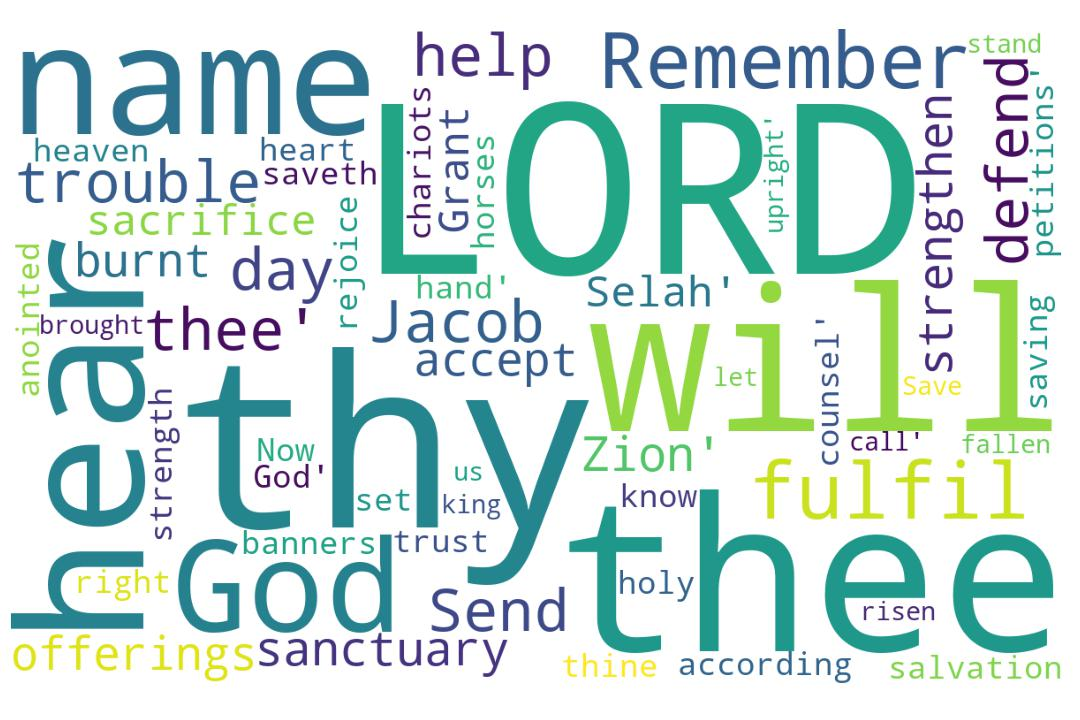
\includegraphics[width=\linewidth]{19OT-Psalms/Psalm20-WordCloud.jpg}
  \caption{Psalm 20 Word Cloud}
  \label{fig:Psalm 20 word Cloud}
\end{figure}

\marginpar{\scriptsize \centering \fcolorbox{bone}{lime}{\textbf{MY SAVIOUR}}\\ (Psalm 20:1-9) \begin{compactenum}[I.][8]
    \item Is a Savior that \textbf{Hears} \index[scripture]{Psalms!Psa 020:01}\index[scripture]{Psalms!Psa 020:09}(Psa 20:1,9)
    \item Is a Savior that \textbf{Helps} \index[scripture]{Psalms!Psa 020:02}(Psa 20:2)
    \item Is a Savior that \textbf{Honors} \index[scripture]{Psalms!Psa 020:03}(Psa 20:3)
    \item Is a Savior that has a \textbf{Heart} for his People \index[scripture]{Psalms!Psa 020:04}\index[scripture]{Psalms!Psa 020:04}(Psa 20:4)
    \item Is a Savior that provids \textbf{Hope} \index[scripture]{Psalms!Psa 020:05}(Psa 20:5)
    \item Is a Savior that has a \textbf{Heritage}  \index[scripture]{Psalms!Psa 020:06}(Psa 20:6)
    \item Is a Savior that is on \textbf{High}  \index[scripture]{Psalms!Psa 020:06}(Psa 20:6)
\end{compactenum}}

\footnote{\textcolor[cmyk]{0.99998,1,0,0}{\hyperlink{TOC}{Return to end of Table of Contents.}}}\footnote{\href{https://www.audioverse.org/english/audiobibles/books/ENGKJV/O/Ps/1}{\textcolor[cmyk]{0.99998,1,0,0}{Psalms Audio}}}\textcolor[cmyk]{0.99998,1,0,0}{To the chief Musician, A Psalm of David.}\\
\\
\textcolor[cmyk]{0.99998,1,0,0}{The LORD \fcolorbox{bone}{lime}{hear} thee in the day of trouble; the name of the God of Jacob defend thee;}\footnote{\textbf{Daniel 12:1} -- And at that time shall Michael stand up, the great prince which standeth for the children of thy people: and there shall be a time of trouble, such as never was since there was a nation \emph{even} to that same time: and at that time thy people shall be delivered, every one that shall be found written in the book.}\footnote{\textbf{Matthew 24:21} -- For then shall be great tribulation, such as was not since the beginning of the world to this time, no, nor ever shall be.}
[2] \textcolor[cmyk]{0.99998,1,0,0}{Send thee \fcolorbox{bone}{lime}{help} from the sanctuary, and strengthen thee out of Zion;}
[3] \textcolor[cmyk]{0.99998,1,0,0}{Remember all \fcolorbox{bone}{lime}{thy offerings}, and accept thy burnt sacrifice; Selah.}
[4] \textcolor[cmyk]{0.99998,1,0,0}{Grant thee according to thine own \fcolorbox{bone}{lime}{heart}, and fulfil all thy counsel.}
[5] \textcolor[cmyk]{0.99998,1,0,0}{We will rejoice in thy salvation, and in the name of our God we will set up \emph{our} banners: the LORD \fcolorbox{bone}{lime}{fulfil} all thy petitions.}
[6] \textcolor[cmyk]{0.99998,1,0,0}{Now know I that the LORD saveth his anointed; he will hear him from his holy heaven with the saving strength of his right hand.}\footnote{\textbf{Psalm 17:7} -- Shew thy marvellous lovingkindness, O thou that savest by thy right hand them which put their trust \emph{in thee} from those that rise up \emph{against them.}}\footnote{\textbf{Psalm 139:10} -- Even there shall thy hand lead me, and thy right hand shall hold me.}
[7] \textcolor[cmyk]{0.99998,1,0,0}{Some \emph{trust} in chariots, and some in horses: but we will remember the name of the LORD our God.}\footnote{Kidner points out that while chariots and horses were the most formidable force of ancient times, here the verse induces memories of Israel's vicotries at the Red Sea (Exodus 14) and at the river Kishon (Judges 4). but we will remember the name of the LORD our God. \cite{kidner2014psalmsV1} }\footnote{\textbf{Exodus 14:28-29} -- And the waters returned, and covered the chariots, and the horsemen, and all the host of Pharaoh that came into the sea after them; there remained not so much as one of them. [29] But the children of Israel walked upon dry land in the midst of the sea; and the waters were a wall unto them on their right hand, and on their left.}\footnote{\textbf{Judges 4:15-15} -- And the LORD discomfited Sisera, and all his chariots, and all his host, with the edge of the sword before Barak; so that Sisera lighted down off his chariot, and fled away on his feet. [16] But Barak pursued after the chariots, and after the host, unto Harosheth of the Gentiles: and all the host of Sisera fell upon the edge of the sword; and there was not a man left.} 
[8] \textcolor[cmyk]{0.99998,1,0,0}{They are brought down and fallen: but we are risen, and stand upright.}
[9] \textcolor[cmyk]{0.99998,1,0,0}{Save, LORD: let the king \fcolorbox{bone}{lime}{hear} us when we call.}

\section{Psalm 20 Comments}

\subsection{Numeric Nuggets}
\textbf{13:} Verse 8 has 13 words. Verse 1 has 13 unique words.


\subsection{Introduction}


From Ruckman, we get the synopsis of the chapter:
\begin{quote}
The entire Psalm is a Second Advent Psalm. “The day of trouble” (vs. 1) is the“time of trouble” (Dan. 12:1; Matt. 24:21) for Israel. And this time the “God of Jacob” is in business. Help must come from the Jewish sanctuary on Mount Zion (vs. 2), where “burnt sacrifices” (vs. 3) are being offered in the Tribulation (see Rev. 11:1–3). Again the word “Selah” shows up to tell us “where we are at.” “Our God,” and “our banners” show the Jewish context (vs. 5). “Thy petitions” can be aimed at a Gentile who is helping the Jew at this time; note the comments of the Holy Spirit on this matter in Deuteronomy 32:43 and Matthew 25:34–42. “His anointed” (vs. 6) has three applications (exactly  as many of the passages in Ps. 19). It is a reference to David personally and historically; it is a reference to the nation of Israel being delivered in the Tribulation. “His right hand” is a reference to the Lord Jesus (see Ps. 17:7, 139:10). The Antichrist is gathering his troops (vs. 7) for the last attack against Israel (see Zech. 14:1–6; Joel 3:11), but “they are brought down and fallen” (vs. 8) at Armageddon (Rev. 19:20), while it is Israel that rises and stands upright (Isa. 2, 9, 65–66). At that time, Deuteronomy 32:43 will be fulfilled to the jot and tittle. “Let the king hear us when we call” (vs. 9). It is the King of kings—a Jewish King— for “salvation is of the JEWS” (John 4:22). The “us” in the passage is the “us” of Psalm 122 and 124. Nothing is difficult anywhere in the Psalm. The Wycliffe commentator misses the import of every single verse in it, and so do the “New” Bible commentators (Yates and Motyer). \cite{Ruckman1992PsalmsV1}\\
\\
From a devotional standpoint: “May the Lord hear me and defend me’’ (vs. 1). “May the Lord strengthen me and send help”  (vs. 2). “May the Lord remember me and accept me” (vs. 3). And “May the Lord answer me and fulfil my request” (vs. 4. See 21:2). The “name” (vs. 7) has salvation in it (“Jesus”); what need then of “chariots and horses?” Some may substitute “fuel and energy” for “chariots and horses,” while others substitute “tanks and planes”; it comes out the same way. “Let the king hear us when we call.” We don’t want anyone else to answer the phone; we don’t want any “disconnections” while conversing; we don’t want to get a busy signal for twenty minutes at a time, and we do not want any “operator” interrupting our conversation. “Let the king hear us when we call.”
\end{quote}

%\index[NWIV]{18!Psalms!Psa 20:1}\index[AWIP]{The!Psalms!Psa 20:1}\index[AWIP]{LORD!Psalms!Psa 20:1}\index[AWIP]{hear!Psalms!Psa 20:1}\index[AWIP]{thee!Psalms!Psa 20:1}\index[AWIP]{thee!Psalms!Psa 20:1 (2)}\index[AWIP]{in!Psalms!Psa 20:1}\index[AWIP]{the!Psalms!Psa 20:1}\index[AWIP]{the!Psalms!Psa 20:1 (2)}\index[AWIP]{the!Psalms!Psa 20:1 (3)}\index[AWIP]{day!Psalms!Psa 20:1}\index[AWIP]{of!Psalms!Psa 20:1}\index[AWIP]{of!Psalms!Psa 20:1 (2)}\index[AWIP]{of!Psalms!Psa 20:1 (3)}\index[AWIP]{trouble!Psalms!Psa 20:1}\index[AWIP]{name!Psalms!Psa 20:1}\index[AWIP]{God!Psalms!Psa 20:1}\index[AWIP]{Jacob!Psalms!Psa 20:1}\index[AWIP]{defend!Psalms!Psa 20:1}

\index[NWIV]{12!Psalms!Psa 20:2}\index[AWIP]{Send!Psalms!Psa 20:2}\index[AWIP]{thee!Psalms!Psa 20:2}\index[AWIP]{thee!Psalms!Psa 20:2 (2)}\index[AWIP]{help!Psalms!Psa 20:2}\index[AWIP]{from!Psalms!Psa 20:2}\index[AWIP]{the!Psalms!Psa 20:2}\index[AWIP]{sanctuary!Psalms!Psa 20:2}\index[AWIP]{and!Psalms!Psa 20:2}\index[AWIP]{strengthen!Psalms!Psa 20:2}\index[AWIP]{out!Psalms!Psa 20:2}\index[AWIP]{of!Psalms!Psa 20:2}\index[AWIP]{Zion!Psalms!Psa 20:2}

\index[NWIV]{10!Psalms!Psa 20:3}\index[AWIP]{Remember!Psalms!Psa 20:3}\index[AWIP]{all!Psalms!Psa 20:3}\index[AWIP]{thy!Psalms!Psa 20:3}\index[AWIP]{thy!Psalms!Psa 20:3 (2)}\index[AWIP]{offerings!Psalms!Psa 20:3}\index[AWIP]{and!Psalms!Psa 20:3}\index[AWIP]{accept!Psalms!Psa 20:3}\index[AWIP]{burnt!Psalms!Psa 20:3}\index[AWIP]{sacrifice!Psalms!Psa 20:3}\index[AWIP]{Selah!Psalms!Psa 20:3}

\index[NWIV]{12!Psalms!Psa 20:4}\index[AWIP]{Grant!Psalms!Psa 20:4}\index[AWIP]{thee!Psalms!Psa 20:4}\index[AWIP]{according!Psalms!Psa 20:4}\index[AWIP]{to!Psalms!Psa 20:4}\index[AWIP]{thine!Psalms!Psa 20:4}\index[AWIP]{own!Psalms!Psa 20:4}\index[AWIP]{heart!Psalms!Psa 20:4}\index[AWIP]{and!Psalms!Psa 20:4}\index[AWIP]{fulfil!Psalms!Psa 20:4}\index[AWIP]{all!Psalms!Psa 20:4}\index[AWIP]{thy!Psalms!Psa 20:4}\index[AWIP]{counsel!Psalms!Psa 20:4}

\index[NWIV]{25!Psalms!Psa 20:5}\index[AWIP]{We!Psalms!Psa 20:5}\index[AWIP]{will!Psalms!Psa 20:5}\index[AWIP]{will!Psalms!Psa 20:5 (2)}\index[AWIP]{rejoice!Psalms!Psa 20:5}\index[AWIP]{in!Psalms!Psa 20:5}\index[AWIP]{in!Psalms!Psa 20:5 (2)}\index[AWIP]{thy!Psalms!Psa 20:5}\index[AWIP]{thy!Psalms!Psa 20:5 (2)}\index[AWIP]{salvation!Psalms!Psa 20:5}\index[AWIP]{and!Psalms!Psa 20:5}\index[AWIP]{the!Psalms!Psa 20:5}\index[AWIP]{the!Psalms!Psa 20:5 (2)}\index[AWIP]{name!Psalms!Psa 20:5}\index[AWIP]{of!Psalms!Psa 20:5}\index[AWIP]{our!Psalms!Psa 20:5}\index[AWIP]{God!Psalms!Psa 20:5}\index[AWIP]{we!Psalms!Psa 20:5}\index[AWIP]{set!Psalms!Psa 20:5}\index[AWIP]{up!Psalms!Psa 20:5}\index[AWIP]{\emph{our}!Psalms!Psa 20:5}\index[AWIP]{banners!Psalms!Psa 20:5}\index[AWIP]{LORD!Psalms!Psa 20:5}\index[AWIP]{fulfil!Psalms!Psa 20:5}\index[AWIP]{all!Psalms!Psa 20:5}\index[AWIP]{petitions!Psalms!Psa 20:5}\index[AWIP]{\emph{our}!Psalms!Psa 20:5}

\index[NWIV]{25!Psalms!Psa 20:6}\index[AWIP]{Now!Psalms!Psa 20:6}\index[AWIP]{know!Psalms!Psa 20:6}\index[AWIP]{I!Psalms!Psa 20:6}\index[AWIP]{that!Psalms!Psa 20:6}\index[AWIP]{the!Psalms!Psa 20:6}\index[AWIP]{the!Psalms!Psa 20:6 (2)}\index[AWIP]{LORD!Psalms!Psa 20:6}\index[AWIP]{saveth!Psalms!Psa 20:6}\index[AWIP]{his!Psalms!Psa 20:6}\index[AWIP]{his!Psalms!Psa 20:6 (2)}\index[AWIP]{his!Psalms!Psa 20:6 (3)}\index[AWIP]{anointed!Psalms!Psa 20:6}\index[AWIP]{he!Psalms!Psa 20:6}\index[AWIP]{will!Psalms!Psa 20:6}\index[AWIP]{hear!Psalms!Psa 20:6}\index[AWIP]{him!Psalms!Psa 20:6}\index[AWIP]{from!Psalms!Psa 20:6}\index[AWIP]{holy!Psalms!Psa 20:6}\index[AWIP]{heaven!Psalms!Psa 20:6}\index[AWIP]{with!Psalms!Psa 20:6}\index[AWIP]{saving!Psalms!Psa 20:6}\index[AWIP]{strength!Psalms!Psa 20:6}\index[AWIP]{of!Psalms!Psa 20:6}\index[AWIP]{right!Psalms!Psa 20:6}\index[AWIP]{hand!Psalms!Psa 20:6}

\index[NWIV]{19!Psalms!Psa 20:7}\index[AWIP]{Some!Psalms!Psa 20:7}\index[AWIP]{\emph{trust}!Psalms!Psa 20:7}\index[AWIP]{in!Psalms!Psa 20:7}\index[AWIP]{in!Psalms!Psa 20:7 (2)}\index[AWIP]{chariots!Psalms!Psa 20:7}\index[AWIP]{and!Psalms!Psa 20:7}\index[AWIP]{some!Psalms!Psa 20:7}\index[AWIP]{horses!Psalms!Psa 20:7}\index[AWIP]{but!Psalms!Psa 20:7}\index[AWIP]{we!Psalms!Psa 20:7}\index[AWIP]{will!Psalms!Psa 20:7}\index[AWIP]{remember!Psalms!Psa 20:7}\index[AWIP]{the!Psalms!Psa 20:7}\index[AWIP]{the!Psalms!Psa 20:7 (2)}\index[AWIP]{name!Psalms!Psa 20:7}\index[AWIP]{of!Psalms!Psa 20:7}\index[AWIP]{LORD!Psalms!Psa 20:7}\index[AWIP]{our!Psalms!Psa 20:7}\index[AWIP]{God!Psalms!Psa 20:7}\index[AWIP]{\emph{trust}!Psalms!Psa 20:7}

\index[NWIV]{13!Psalms!Psa 20:8}\index[AWIP]{They!Psalms!Psa 20:8}\index[AWIP]{are!Psalms!Psa 20:8}\index[AWIP]{are!Psalms!Psa 20:8 (2)}\index[AWIP]{brought!Psalms!Psa 20:8}\index[AWIP]{down!Psalms!Psa 20:8}\index[AWIP]{and!Psalms!Psa 20:8}\index[AWIP]{and!Psalms!Psa 20:8 (2)}\index[AWIP]{fallen!Psalms!Psa 20:8}\index[AWIP]{but!Psalms!Psa 20:8}\index[AWIP]{we!Psalms!Psa 20:8}\index[AWIP]{risen!Psalms!Psa 20:8}\index[AWIP]{stand!Psalms!Psa 20:8}\index[AWIP]{upright!Psalms!Psa 20:8}

\index[NWIV]{10!Psalms!Psa 20:9}\index[AWIP]{Save!Psalms!Psa 20:9}\index[AWIP]{LORD!Psalms!Psa 20:9}\index[AWIP]{let!Psalms!Psa 20:9}\index[AWIP]{the!Psalms!Psa 20:9}\index[AWIP]{king!Psalms!Psa 20:9}\index[AWIP]{hear!Psalms!Psa 20:9}\index[AWIP]{us!Psalms!Psa 20:9}\index[AWIP]{when!Psalms!Psa 20:9}\index[AWIP]{we!Psalms!Psa 20:9}\index[AWIP]{call!Psalms!Psa 20:9}


\section{Psalm 20 Outlines}

\subsection{My Outlines}

\subsubsection{My Savior}
%\textbf{Introduction:} Psalm 20:
\index[speaker]{Keith Anthony!Psalm 020 (My Savior)}
\index[series]{Psalms (Keith Anthony)!Psalm 020 (My Savior)}
\index[date]{2016/06/26!Psalm 020 (My Savior) (Keith Anthony)}

\begin{compactenum}[I.][7]
    \item Is a Savior that \textbf{Hears} \index[scripture]{Psalms!Psa 020:01}\index[scripture]{Psalms!Psa 020:09}(Psa 20:1,9)
    \item Is a Savior that \textbf{Helps} \index[scripture]{Psalms!Psa 020:02}(Psa 20:2)
    \item Is a Savior that \textbf{Honors} \index[scripture]{Psalms!Psa 020:03}(Psa 20:3)
    \item Is a Savior that has a \textbf{Heart} for his People \index[scripture]{Psalms!Psa 020:04}\index[scripture]{Psalms!Psa 020:04}(Psa 20:4)
    \item Is a Savior that provids \textbf{Hope} \index[scripture]{Psalms!Psa 020:05}(Psa 20:5)
    \item Is a Savior that has a \textbf{Heritage}  \index[scripture]{Psalms!Psa 020:06}(Psa 20:6)
    \item Is a Savior that is on \textbf{High}  \index[scripture]{Psalms!Psa 020:06}(Psa 20:6)
\end{compactenum} 



\subsection{Outlines from Others}

\subsubsection{Eight Words to Pray}
\index[speaker]{Jim Irwin!Psalm 020 (Eight Words to Pray)}
\index[series]{Psalms (Jim Irwin)!Psalm 020 (Eight Words to Pray)}
\index[date]{2016/04/16!Psalm 020 (Eight Words to Pray) (Jim Irwin)}
\textbf{Introduction: }Living next to the Gulf Coast has sensitized me to “the calm before the storm,” that eerie moment of silence just before the winds and rains crash in upon us. The skies become leaden. The wind subsides momentarily. The smell of rain is in the air. It is as if nature pauses before its holocaust breaks loose. Similarly, life has its moments of calm. Battlefields lie quiet; then the bombardment begins. Anxious reporters freeze as news of the president’s condition comes from the emergency room. Marital strain can grip a family in silence before the cracks appear. Psalm 20 is such a pause. Israel is ready for battle; the “day of trouble” has come. The legions with their banners are ordered for war. But while pagans trust in chariots and horses, God’s people trust in His name. In “the calm before the storm,” the commanders go up to the temple with their troops where the king offers his sacrifice and Israel is blessed for battle. Only when spiritual preparation is completed can the opposing forces be joined. Many people want to have victory in life. They want to see success in everything they do. Here, David prays for victory in the oncoming battle. He asks for God to hand him victory. He admits that other people trust in other things to gain victory. David only trusts God. But just because he doesn’t trust in other ways for success, that doesn’t prevent him from making the “big ask.” Eight times, David claims that God can do something for him to provide him victory. David prayed to God for victory in his circumstances. God helped him. David was in a very tight spot. But God helped him. Just as God helped David, He can also help you. I agree with John Calvin about this psalm. He said: Many interpreters view this prayer as offered up only on one particular occasion; but in this I cannot agree. The occasion of its composition at first may have arisen from some particular battle which was about to be fought, either against the Ammonites, or against some other enemies of Israel. But the design of the Holy Spirit, in my judgment, was to deliver to the Church a common form of prayer, which, as we may gather from the words, was to be used whenever she was threatened with any danger. These requests were from a king who was ready for battle against a national foe. I believe that we can personalize these requests from a child of a king who is ready for battle against a spiritual foe. So I want us to look at these prayers as petitions we can ask from God in our own lives. \href{http://www.patheos.com/blogs/jimerwin/2016/04/18/psalm-201-9-trusting-god-prayer/\#Mgi8KGIip8tAbGeA.99}{Read more.}
\begin{compactenum}[I.][8]
    \item \textbf{Answer} Me \index[scripture]{Psalms!Psa 020:01}\index[scripture]{Psalms!Psa 020:09}(Psalm 20:1,9)
    \item \textbf{Protect} Me \index[scripture]{Psalms!Psa 020:01}(Psalm 20:1)
    \item \textbf{Help} Me \index[scripture]{Psalms!Psa 020:02}(Psalm 20:2)
    \item \textbf{Sustain} Me \index[scripture]{Psalms!Psa 020:02}(Psalm 20:2)
    \item \textbf{Remember} Me \index[scripture]{Psalms!Psa 020:03}(Psalm 20:3)
    \item \textbf{Give} Me \index[scripture]{Psalms!Psa 020:04}(Psalm 20:4)
    \item \textbf{Fulfill} Me \index[scripture]{Psalms!Psa 020:04}(Psalm 20:4)
    \item \textbf{Lift} Me \index[scripture]{Psalms!Psa 020:05--08}(Psalm 20:5--8)
\end{compactenum} 

%\section{Psalm 20 Word Statistics}


%%%%%%%%%%
%%%%%%%%%%
\normalsize
 
\begin{center}
\begin{longtable}{l|c|c|c|c}
\caption[Psalm 20 Statistics]{Psalm 20 Statistics}\label{table:Statistics for Psalm 20} \\
\hline \multicolumn{1}{|c|}{\textbf{Verse(s)}} & \multicolumn{1}{|c|}{\textbf{Count}} & \multicolumn{1}{|c|}{\textbf{Unique}} & \multicolumn{1}{|c|}{\textbf{Italics}} & \multicolumn{1}{|c|}{\textbf{Uniq Italic}}  \\ \hline 
\endfirsthead
 
\multicolumn{5}{c}
{{\bfseries \tablename\ \thetable{} -- continued from previous page}} \\  
\hline \multicolumn{1}{|c|}{\textbf{Verse(s)}} & \multicolumn{1}{|c|}{\textbf{Count}} & \multicolumn{1}{|c|}{\textbf{Unique}} & \multicolumn{1}{|c|}{\textbf{Italics}} & \multicolumn{1}{|c|}{\textbf{Uniq Italic}}  \\ \hline 
\endhead
 
\hline \multicolumn{5}{|r|}{{Continued if needed}} \\ \hline
\endfoot 
1 & 18 & 13 & 0 & 0\\ \hline
2 & 12 & 11 & 0 & 0\\ \hline
3 & 10 & 9 & 0 & 0\\ \hline
4 & 12 & 12 & 0 & 0\\ \hline
5 & 25 & 21 & 1 & 1\\ \hline
6 & 25 & 22 & 0 & 0\\ \hline
7 & 19 & 17 & 1 & 1\\ \hline
8 & 13 & 11 & 0 & 0\\ \hline
9 & 10 & 10 & 0 & 0\\ \hline
Total & 144 & 85 & 2 & 2
\end{longtable}
\end{center}



%%%%%%%%%%
%%%%%%%%%%


\subsection{Psalm 20 Words by Frequency}


%%%%%%%%%%
%%%%%%%%%%
\normalsize
 
\begin{center}
\begin{longtable}{l|r}
\caption[Psalm 20 Words by Frequency]{Psalm 20 Words by Frequency}\label{table:WordsbyFrequency for Psalm 20} \\
\hline \multicolumn{1}{|c|}{\textbf{Word}} & \multicolumn{1}{c|}{\textbf{Frequency}} \\ \hline 
\endfirsthead
 
\multicolumn{2}{c}
{{\bfseries \tablename\ \thetable{} -- continued from previous page}} \\  
\hline \multicolumn{1}{|c|}{\textbf{Word}} & \multicolumn{1}{c|}{\textbf{Frequency}} \\ \hline 
\endhead
 
\hline \multicolumn{2}{c}{{ }} \\ \hline
\endfoot 
the & 11\\ \hline 
of & 7\\ \hline 
and & 7\\ \hline 
LORD & 5\\ \hline 
thee & 5\\ \hline 
in & 5\\ \hline 
thy & 5\\ \hline 
will & 4\\ \hline 
we & 4\\ \hline 
hear & 3\\ \hline 
name & 3\\ \hline 
God & 3\\ \hline 
all & 3\\ \hline 
his & 3\\ \hline 
from & 2\\ \hline 
fulfil & 2\\ \hline 
our & 2\\ \hline 
but & 2\\ \hline 
are & 2\\ \hline 
The & 1\\ \hline 
day & 1\\ \hline 
trouble & 1\\ \hline 
Jacob & 1\\ \hline 
defend & 1\\ \hline 
Send & 1\\ \hline 
help & 1\\ \hline 
sanctuary & 1\\ \hline 
strengthen & 1\\ \hline 
out & 1\\ \hline 
Zion & 1\\ \hline 
Remember & 1\\ \hline 
offerings & 1\\ \hline 
accept & 1\\ \hline 
burnt & 1\\ \hline 
sacrifice & 1\\ \hline 
Selah & 1\\ \hline 
Grant & 1\\ \hline 
according & 1\\ \hline 
to & 1\\ \hline 
thine & 1\\ \hline 
own & 1\\ \hline 
heart & 1\\ \hline 
counsel & 1\\ \hline 
We & 1\\ \hline 
rejoice & 1\\ \hline 
salvation & 1\\ \hline 
set & 1\\ \hline 
up & 1\\ \hline 
\emph{our} & 1\\ \hline 
banners & 1\\ \hline 
petitions & 1\\ \hline 
Now & 1\\ \hline 
know & 1\\ \hline 
I & 1\\ \hline 
that & 1\\ \hline 
saveth & 1\\ \hline 
anointed & 1\\ \hline 
he & 1\\ \hline 
him & 1\\ \hline 
holy & 1\\ \hline 
heaven & 1\\ \hline 
with & 1\\ \hline 
saving & 1\\ \hline 
strength & 1\\ \hline 
right & 1\\ \hline 
hand & 1\\ \hline 
Some & 1\\ \hline 
\emph{trust} & 1\\ \hline 
chariots & 1\\ \hline 
some & 1\\ \hline 
horses & 1\\ \hline 
remember & 1\\ \hline 
They & 1\\ \hline 
brought & 1\\ \hline 
down & 1\\ \hline 
fallen & 1\\ \hline 
risen & 1\\ \hline 
stand & 1\\ \hline 
upright & 1\\ \hline 
Save & 1\\ \hline 
let & 1\\ \hline 
king & 1\\ \hline 
us & 1\\ \hline 
when & 1\\ \hline 
call & 1\\ \hline 
\end{longtable}
\end{center}



%%%%%%%%%%
%%%%%%%%%%


\subsection{Psalm 20 Words Alphabetically}


%%%%%%%%%%
%%%%%%%%%%
\normalsize
 
\begin{center}
\begin{longtable}{l|r}
\caption[Psalm 20 Words Alphabetically]{Psalm 20 Words Alphabetically}\label{table:WordsAlphabetically for Psalm 20} \\
\hline \multicolumn{1}{|c|}{\textbf{Word}} & \multicolumn{1}{c|}{\textbf{Frequency}} \\ \hline 
\endfirsthead
 
\multicolumn{2}{c}
{{\bfseries \tablename\ \thetable{} -- continued from previous page}} \\  
\hline \multicolumn{1}{|c|}{\textbf{Word}} & \multicolumn{1}{c|}{\textbf{Frequency}} \\ \hline 
\endhead
 
\hline \multicolumn{2}{c}{{ }} \\ \hline
\endfoot 
God & 3\\ \hline 
Grant & 1\\ \hline 
I & 1\\ \hline 
Jacob & 1\\ \hline 
LORD & 5\\ \hline 
Now & 1\\ \hline 
Remember & 1\\ \hline 
Save & 1\\ \hline 
Selah & 1\\ \hline 
Send & 1\\ \hline 
Some & 1\\ \hline 
The & 1\\ \hline 
They & 1\\ \hline 
We & 1\\ \hline 
Zion & 1\\ \hline 
\emph{our} & 1\\ \hline 
\emph{trust} & 1\\ \hline 
accept & 1\\ \hline 
according & 1\\ \hline 
all & 3\\ \hline 
and & 7\\ \hline 
anointed & 1\\ \hline 
are & 2\\ \hline 
banners & 1\\ \hline 
brought & 1\\ \hline 
burnt & 1\\ \hline 
but & 2\\ \hline 
call & 1\\ \hline 
chariots & 1\\ \hline 
counsel & 1\\ \hline 
day & 1\\ \hline 
defend & 1\\ \hline 
down & 1\\ \hline 
fallen & 1\\ \hline 
from & 2\\ \hline 
fulfil & 2\\ \hline 
hand & 1\\ \hline 
he & 1\\ \hline 
hear & 3\\ \hline 
heart & 1\\ \hline 
heaven & 1\\ \hline 
help & 1\\ \hline 
him & 1\\ \hline 
his & 3\\ \hline 
holy & 1\\ \hline 
horses & 1\\ \hline 
in & 5\\ \hline 
king & 1\\ \hline 
know & 1\\ \hline 
let & 1\\ \hline 
name & 3\\ \hline 
of & 7\\ \hline 
offerings & 1\\ \hline 
our & 2\\ \hline 
out & 1\\ \hline 
own & 1\\ \hline 
petitions & 1\\ \hline 
rejoice & 1\\ \hline 
remember & 1\\ \hline 
right & 1\\ \hline 
risen & 1\\ \hline 
sacrifice & 1\\ \hline 
salvation & 1\\ \hline 
sanctuary & 1\\ \hline 
saveth & 1\\ \hline 
saving & 1\\ \hline 
set & 1\\ \hline 
some & 1\\ \hline 
stand & 1\\ \hline 
strength & 1\\ \hline 
strengthen & 1\\ \hline 
that & 1\\ \hline 
the & 11\\ \hline 
thee & 5\\ \hline 
thine & 1\\ \hline 
thy & 5\\ \hline 
to & 1\\ \hline 
trouble & 1\\ \hline 
up & 1\\ \hline 
upright & 1\\ \hline 
us & 1\\ \hline 
we & 4\\ \hline 
when & 1\\ \hline 
will & 4\\ \hline 
with & 1\\ \hline 
\end{longtable}
\end{center}



%%%%%%%%%%
%%%%%%%%%%


\subsection{Psalm 20 Words by Length}


%%%%%%%%%%
%%%%%%%%%%
\normalsize
 
\begin{center}
\begin{longtable}{l|p{3.75in}}
\caption[Psalm 20 Words by Length]{Psalm 20 Words by Length}\label{table:WordsAlphabetically for Psalm 20} \\
\hline \multicolumn{1}{|c|}{\textbf{Length}} & \multicolumn{1}{c|}{\textbf{Words}} \\ \hline 
\endfirsthead
\hline \multicolumn{1}{|c|}{\textbf{Length}} & \multicolumn{1}{c|}{\textbf{Words}} \\ \hline 
\multicolumn{2}{c}
{{\bfseries \tablename\ \thetable{} -- continued from previous page}} \\  
\hline \multicolumn{1}{|c|}{\textbf{Word}} & \multicolumn{1}{c|}{\textbf{Frequency}} \\ \hline 
\endhead
 
\hline \multicolumn{2}{c}{{ }} \\ \hline
\endfoot 
1 & I\\ \hline 
2 & in, of, to, We, we, up, he, us\\ \hline 
3 & The, the, day, God, and, out, all, thy, own, our, set, \emph{our}, Now, his, him, but, are, let\\ \hline 
4 & LORD, hear, thee, name, Send, help, from, Zion, will, know, that, holy, with, hand, Some, some, They, down, Save, king, when, call\\ \hline 
5 & Jacob, burnt, Selah, Grant, thine, heart, right, \emph{trust}, risen, stand\\ \hline 
6 & defend, accept, fulfil, saveth, heaven, saving, horses, fallen\\ \hline 
7 & trouble, counsel, rejoice, banners, brought, upright\\ \hline 
8 & Remember, anointed, strength, chariots, remember\\ \hline 
9 & sanctuary, offerings, sacrifice, according, salvation, petitions\\ \hline 
10 & strengthen\\ \hline 
\end{longtable}
\end{center}



%%%%%%%%%%
%%%%%%%%%%



\subsection{Psalm 20 Repeated Phrases}


%%%%%%%%%%
%%%%%%%%%%
\normalsize
 
\begin{center}
\begin{longtable}{|p{3.0in}|p{0.5in}|}
\caption[Psalm 20 Repeated Phrases]{Psalm 20 Repeated Phrases}\label{table:Repeated Phrases Psalm 20} \\
\hline \multicolumn{1}{|c|}{\textbf{Phrase}} & \multicolumn{1}{c|}{\textbf{Frequency}} \\ \hline 
\endfirsthead
 
\multicolumn{2}{c}
{{\bfseries \tablename\ \thetable{} -- continued from previous page}} \\  
\hline \multicolumn{1}{|c|}{\textbf{Phrase}} & \multicolumn{1}{c|}{\textbf{Frequency}} \\ \hline 
\endhead
 
\hline \multicolumn{2}{c}{{ }} \\ \hline
\endfoot 
the name & 3\\ \hline 
the name of & 3\\ \hline 
name of & 3\\ \hline 
all thy & 3\\ \hline 
the LORD & 3\\ \hline 
\end{longtable}
\end{center}



%%%%%%%%%%
%%%%%%%%%%




\chapter{Psalm 21}

\begin{figure}
  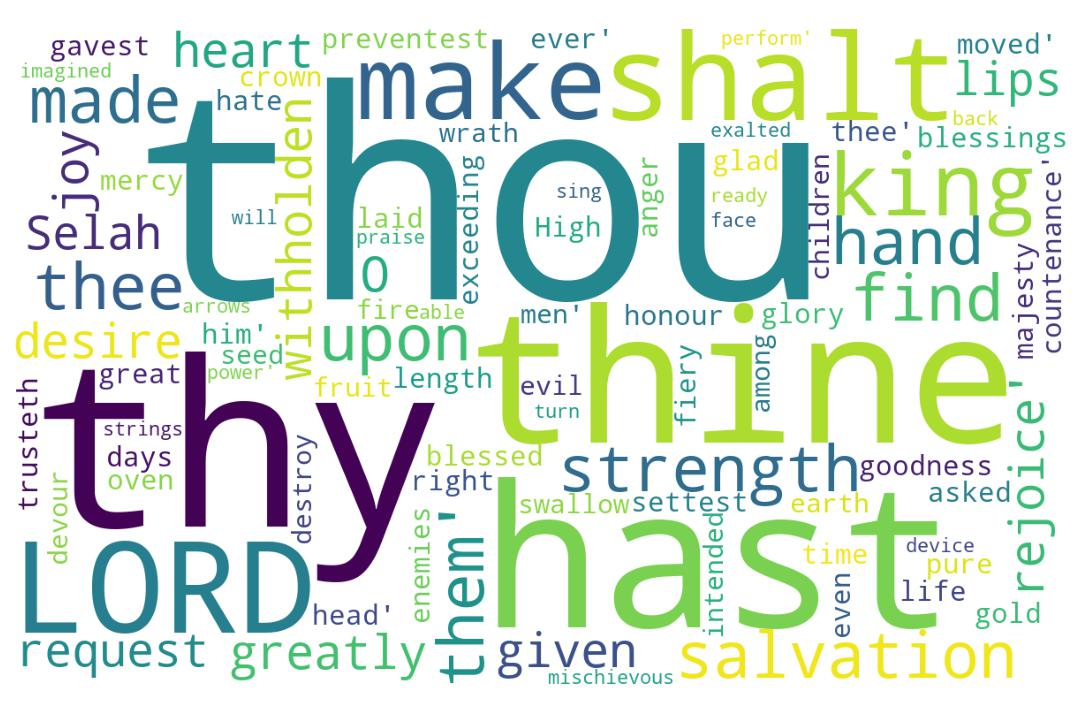
\includegraphics[width=\linewidth]{19OT-Psalms/Psalm21-WordCloud.jpg}
  \caption{Psalm 21 Word Cloud}
  \label{fig:Psalm 21 word Cloud}
\end{figure}

\marginpar{\scriptsize \centering \fcolorbox{bone}{lime}{\textbf{A GLIMPSE OF THE KING}}\\ (Psalm 21:1--13) \begin{compactenum}[I.][8]
    \item He has \textbf{Eternal Life} \index[scripture]{Psalms!Psa 021:04}(Psa 21:4)
    \item He has \textbf{Exceeding Glory} \index[scripture]{Psalms!Psa 021:05}(Psa 21:5)
    \item He has \textbf{Endless Majesty \& Honor} \index[scripture]{Psalms!Psa 021:05}(Psa 21:5)
    \item He has \textbf{Everlasting Blessing} \index[scripture]{Psalms!Psa 021:06}(Psa 21:6)
    \item He has \textbf{Enemies Destroyed} \index[scripture]{Psalms!Psa 021:08-10}(Psa 21:8-10)
    \item He has \textbf{Enormous Power} \index[scripture]{Psalms!Psa 021:13}(Psa 21:13)
\end{compactenum}}

\footnote{\textcolor[cmyk]{0.99998,1,0,0}{\hyperlink{TOC}{Return to end of Table of Contents.}}}\footnote{\href{https://www.audioverse.org/english/audiobibles/books/ENGKJV/O/Ps/1}{\textcolor[cmyk]{0.99998,1,0,0}{Psalms Audio}}}\textcolor[cmyk]{0.99998,1,0,0}{To the chief Musician, A Psalm of David.}\\
\\
\textcolor[cmyk]{0.99998,1,0,0}{The king shall joy in thy strength, O LORD; and in thy salvation how greatly shall he rejoice!}
[2] \textcolor[cmyk]{0.99998,1,0,0}{Thou hast given him his heart's desire, and hast not withholden the request of his lips. Selah.}\footnote{\textbf{Psalm 10:3} - For the wicked boasteth of his heart’s desire, and blesseth the covetous, whom the LORD abhorreth.}\footnote{\textbf{Romans 10:1} - Brethren, my heart’s desire and prayer to God for Israel is, that they might be saved.}
[3] \textcolor[cmyk]{0.99998,1,0,0}{For thou preventest him with the blessings of goodness: thou settest a crown of pure gold on his head.}
[4] \textcolor[cmyk]{0.99998,1,0,0}{He asked life of thee, \emph{and} thou gavest \emph{it} him, \emph{even} length of days \fcolorbox{bone}{lime}{for ever and ever}.}
[5] \textcolor[cmyk]{0.99998,1,0,0}{His \fcolorbox{bone}{lime}{glory} \emph{is} great in thy salvation: \fcolorbox{bone}{lime}{honour and} \fcolorbox{bone}{lime}{majesty} hast thou laid upon him.}
[6] \textcolor[cmyk]{0.99998,1,0,0}{For thou hast made him \fcolorbox{bone}{lime}{most blessed} for ever: thou hast made him exceeding glad with thy countenance.}
[7] \textcolor[cmyk]{0.99998,1,0,0}{For the king trusteth in the LORD, and through the mercy of the most High he shall not be moved.}
[8] \textcolor[cmyk]{0.99998,1,0,0}{Thine hand shall find out all thine \fcolorbox{bone}{lime}{enemies}: thy right hand shall find out those that hate thee.}
[9] \textcolor[cmyk]{0.99998,1,0,0}{Thou shalt make them as a fiery oven in the time of thine anger: the LORD shall swallow them up in his wrath, and the fire shall devour them.}
[10] \textcolor[cmyk]{0.99998,1,0,0}{Their fruit shalt thou destroy from the earth, and their seed from among the children of men.}
[11] \textcolor[cmyk]{0.99998,1,0,0}{For they intended evil against thee: they imagined a mischievous device, \emph{which} they are not able \emph{to} \emph{perform}.}\footnote{\textbf{Acts 13:10} - And said, O full of all subtilty and all mischief, thou child of the devil, thou enemy of all righteousness, wilt thou not cease to pervert the right ways of the Lord?}
[12] \textcolor[cmyk]{0.99998,1,0,0}{Therefore shalt thou make them turn their back, \emph{when} thou shalt make ready \emph{thine} \emph{arrows} upon thy strings against the face of them.}
[13] \textcolor[cmyk]{0.99998,1,0,0}{Be thou exalted, LORD, in \fcolorbox{bone}{lime}{thine own strength}: \emph{so} will we sing and praise thy power.}



\section{Psalm 21 Comments}

\subsection{Numeric Nuggets}
\textbf{18:} There are 13 verses in the psalm. Verses 1, 4, 6, 8, and 11 have 18 words. 

\subsection{Psalm 21 Introduction}
The psalm switches back and forth between David's kingship and Christ's kingship.

\subsection{Psalm 21:3}
Read the word ``preventest'' as ``pre-eventest'' - something that happens before something else. Here, the bestowing of goodness came first and then the crown.  Forms of the word ``prevent''a re found 17 times in the, AV, with the most famous probably being 1 Thessalonians 4:15, which speaks of the order of events at the Rapture of the Church.\footnote{\textbf{1 Thessalonians 4:15} - For this we say unto you by the word of the Lord, that we which are alive and remain unto the coming of the Lord shall not prevent them which are asleep.}

\subsection{Psalm 21:11}
The word ``mischievous'' is used 5 times in scripture: (1) Psalms 21:11, (2) Psalms 38:12, (3) Proverbs 24:8, (4) Ecclesiastes 10:13, and (5) Micah 7:3. The sources is identified in Acts 13:10.

%% Ruckman Notes
%% The whole Psalm is about the Lord Jesus Christ, most of it again dealing with His Second Coming and coronation as “King over all the earth” (Zech. 14:9; Ps. 47:2;  Ps.  72). As usual, David switches back and forth from his own kingship to Christ’s kingship. “The king” in verse 1 is David rejoicing in the Lord. He is trusting in the Lord in verse 7 (the theme of the first forty-one Psalms).  But there are overtones in verses 2, 3, and 4 that take us far beyond David. Now, we have spoken at length on verse 4 in The Commentary on the Pastoral Epistle (see Titus 1:1–2). The long and short of it is that in making an ETERNAL payment for sin (which required ETERNAL DEATH) the Lord Jesus Christ was promised ETERNAL LIFE—before Genesis 1:1. David’s “heart’s  desire” may have been to have a son on his throne, but when he is given the “sure promises” of an everlasting seed and throne (2 Sam. 7:16), it comes to him as a complete surprise (2 Sam. 7:18); evidently he had NOT asked for what was given. The words of Psalm 21 are literally true of one man, and one man only. Look at them: 1. He has eternal life (vs. 4). 2. His glory is great (vs. 5). 3. He has honour and majesty (vs. 5) 4. He is blessed forever (vs. 6) 5. God will destroy ALL of His enemies (vss. 8–10). David is speaking of “the King of the Jews” (John 19:19). So in the next Psalm he describes what took place when THAT inscription was placed over the King’s head. Devotionally, we may ask, “Do you ‘greatly rejoice,’ as David, who danced although he was a king?’’ (vs. 1) You need goodness (vs. 3) before you need wealth or health; goodness is a “blessing.” Imagine GOD crowning a MAN (vs. 3) (the only time this ever happened was when Pope Leo crowned Charlemagne, Christmas Eve, A.D. 800, and claimed that “God was doing the crowning.” Heil papa! Vatican über alles!). Note, in verse 4, that eternal life can be had for the ASKING; did you get that? Get it out of Romans 10:13 if you didn’t get it here. If God “ONLY hath immortality” (see 1 Tim. 6:16) then He can give it to sinners (1 Cor. 15:49– 55). “Glory...honour, and majesty” (vs. 5) are either fleshy or demoniac when they are not “sanctified.” Salvation sanctifies “glory...honour, and majesty.” Without salvation (“education without salvation is damnation”) glory, honour, and majesty turn out like they turned out when connected with Caesar Augustus, bloody Mary, Adolph Hitler, Pope Leo the Great, M. L. King Jr., Mandela, Castro, King Henry VIII, Napoleon, Tully, Wallenstein, Marx, Freud, Einstein, FDR, and Pope Paul VI: disruption, demolition, and catastrophe. Alexander  the Great had all three; so did Napoleon and Abraham Lincoln.
%%
%% Verse 9 matches Malachi 4:1–4 and 2 Thessalonians 2:8. John the Baptist makes reference to it in Matthew 3:10, 12. Verse 10 is commented on by the Holy Spirit in Isaiah 14:20, and has to do with the “seed” of the Son of Perdition (cf. also Job 18:19). “They intended evil against thee.” Like Joseph’s brothers (Gen. 50:20) they intended to annihilate the “heir” (see Matt. 21:38). “They imagined a mischievous device” according to Acts 3:14–15 and Acts 2:22–24, but they were “not able to perform” it because the “victim” didn’t stay dead. (“You can’t keep a good man down!”). He rose from the dead (see vs. 4). They planned to run the world without Him. “Evil,” in this case, means: The CFR, NAACP, NEA, AMA, CIA, FBI, HEW, NCCC, UN, League of Nations, Triple Entente, Holy Alliance, NATO Treaty, Warsaw Pact, planned economy, birth control, air conditioning, computers, Vatican politics, the Bilderbergers, Illuminati, Federal Reserve System, ASV, Democratic Party platform, urban renewal, the NASV, affirmative action, revenue sharing, agrarian reforms, the NIV, and “city hall.” All scientific, social, economic, educational, political, and religious “progress” is simply “man” trying to get rid of God (see The Commentary on Genesis: Gen. 3:16–19 and Gen. 9:1–3). They want to run the vineyard (Matt. 21:38). They will not have “this man” to reign over them (Luke 19:14). He will, anyway, for He will “make them turn their back” when He makes ready his arrows “against the face of them” (vs. 12). Jesus Christ will be exalted in His own strength (vs. 13), and then we, along with Israel, will “sing and praise” His power (vs. 13). If He could be exalted only through our strength, God would get no real praise.

%\input{19OT-Psalms/Psalm21WordIndex}
\section{Psalm 21 Outlines}

\subsection{My Outlines}

\subsubsection{A Glimpse of the King}

\index[speaker]{Keith Anthony!Psalm 021 (A Glimpse of the King)}
\index[series]{Psalms (Keith Anthony)!Psalm 021 (A Glimpse of the King)}
\index[date]{2016/06/27!Psalm 021 (A Glimpse of the King) (Keith Anthony)}

\begin{compactenum}[I.][7]
    \item He has \textbf{Eternal Life} \index[scripture]{Psalms!Psa 021:04}(Psa 21:4)
    \item He has \textbf{Exceeding Glory} \index[scripture]{Psalms!Psa 021:05}(Psa 21:5)
    \item He has \textbf{Endless Majesty \& Honor} \index[scripture]{Psalms!Psa 021:05}(Psa 21:5)
    \item He has \textbf{Everlasting Blessing} \index[scripture]{Psalms!Psa 021:06}(Psa 21:6)
    \item He has \textbf{Enemies Destroyed} \index[scripture]{Psalms!Psa 021:08-10}(Psa 21:8-10)
    \item He has \textbf{Enormous Power} \index[scripture]{Psalms!Psa 021:13}(Psa 21:13)
\end{compactenum} 


\subsection{Outlines from Others}

\subsubsection{Crown Him Lord of All}

\index[speaker]{John Phillips!Psalm 021 (Crown Him Lord of All)}
\index[series]{Psalms (John Phillips)!Psalm 021 (Crown Him Lord of All)}
\index[date]{2016/06/27!Psalm 021 (Crown Him Lord of All) (John Phillips)}

\begin{compactenum}[I.][7]
    \item The  \textbf{Secret} of the King's Strength (Expositional) \index[scripture]{Psalms!Psa 021:01-07}(Psalm 21:1-7)
    \begin{compactenum}[A.][2]
        \item The Secret is Disclosed \index[scripture]{Psalms!Psa 021:01-02}(Psalm 21:1-2)
        \begin{compactenum}[1.]
            \item The Publication of the Secret \index[scripture]{Psalms!Psa 021:01}(Psalm 21:1)\footnote{John Phillips}
            \item The Proof of the Secret \index[scripture]{Psalms!Psa 021:02}(Psalm 21:2)
        \end{compactenum}
        \item The Secret is Discussed \index[scripture]{Psalms!Psa 021:03-07}(Psalm 21:3-7) -- the King's Secret Strength Results in
        \begin{compactenum}[1.]
            \item Sovereignty \index[scripture]{Psalms!Psa 021:03}(Psalm 21:3)
            \item Salvation \index[scripture]{Psalms!Psa 021:04-06}(Psalm 21:4-6)
            \item Security \index[scripture]{Psalms!Psa 021:07}(Psalm 21:7)
        \end{compactenum}
    \end{compactenum}
    \item The  \textbf{Sufficiency} of the King's Strength (Experiential) \index[scripture]{Psalms!Psa 021:08-13}(Psalm 21:8-13)
    \begin{compactenum}[A.][2]
        \item A Kingdom Based on the Power of God \index[scripture]{Psalms!Psa 021:08-12}(Psalm 21:8-12)
            \begin{compactenum}[1.]
                \item God's Power to Discover His Foes \index[scripture]{Psalms!Psa 021:08}(Psalm 21:8)
                \item God's Power to Destroy His Foes  \index[scripture]{Psalms!Psa 021:09-12}(Psalm 21:9-12)
                \begin{compactenum}[a.]
                    \item In a Passionate Way \index[scripture]{Psalms!Psa 021:09}(Psalm 21:9) 
                    \item In a Permanent Way \index[scripture]{Psalms!Psa 021:10}(Psalm 21:10) 
                    \item In a Purposeful Way \index[scripture]{Psalms!Psa 021:11-12}(Psalm 21:11-12) 
                \end{compactenum}
            \end{compactenum}
        \item A Kingdom Based on the Preeminence of God \index[scripture]{Psalms!Psa 021:13}(Psalm 21:13)
    \end{compactenum}
\end{compactenum} 


%\section{Psalm 21 Statistics}

%%%%%%%%%%%%%%%%%%%%%%%%%%%
%%%%%Word Statistics
%%%%%%%%%%%%%%%%%%%%%%%%%%%


\normalsize



\subsection{Chapter Word Statistics}


%%%%%%%%%%
%%%%%%%%%%
 
\begin{center}
\begin{longtable}{l|c|c|c|c}
\caption[Stats for Psalm 21]{Stats for Psalm 21} \label{table:Stats for Psalm 21} \\ 
\hline \multicolumn{1}{|c|}{\textbf{Verse(s)}} & \multicolumn{1}{|c|}{\textbf{Count}} & \multicolumn{1}{|c|}{\textbf{Unique}} & \multicolumn{1}{|c|}{\textbf{Italics}} & \multicolumn{1}{|c|}{\textbf{Uniq Italic}}  \\ \hline 
\endfirsthead
 
\multicolumn{5}{c}
{{\bfseries \tablename\ \thetable{} -- continued from previous page}} \\  
\hline \multicolumn{1}{|c|}{\textbf{Verse(s)}} & \multicolumn{1}{|c|}{\textbf{Count}} & \multicolumn{1}{|c|}{\textbf{Unique}} & \multicolumn{1}{|c|}{\textbf{Italics}} & \multicolumn{1}{|c|}{\textbf{Uniq Italic}}  \\ \hline 
\endhead
 
\hline \multicolumn{5}{|r|}{{Continued if needed}} \\ \hline
\endfoot 
1 & 18 & 15 & 0 & 0\\ \hline
2 & 17 & 15 & 0 & 0\\ \hline
3 & 19 & 17 & 0 & 0\\ \hline
4 & 18 & 16 & 3 & 3\\ \hline
5 & 15 & 15 & 1 & 1\\ \hline
6 & 18 & 14 & 0 & 0\\ \hline
7 & 20 & 17 & 0 & 0\\ \hline
8 & 18 & 14 & 0 & 0\\ \hline
9 & 29 & 23 & 0 & 0\\ \hline
10 & 17 & 15 & 0 & 0\\ \hline
11 & 18 & 16 & 3 & 3\\ \hline
12 & 23 & 19 & 3 & 3\\ \hline
13 & 16 & 16 & 1 & 1\\ \hline
\hline \hline
Total & 246 & 138 & 11 & 11



\end{longtable}
\end{center}

%%%%%%%%%%
%%%%%%%%%%
 
\subsection{Words by Frequency}

\begin{center}
\begin{longtable}{l|r}
\caption[Word Frequencies in Psalm 21]{Word Frequencies in Psalm 21} \label{table:WordsIn-Psalm-21} \\ 
\hline \multicolumn{1}{|c|}{\textbf{Word}} & \multicolumn{1}{c|}{\textbf{Frequency}} \\ \hline 
\endfirsthead
 
\multicolumn{2}{c}
{{\bfseries \tablename\ \thetable{} -- continued from previous page}} \\ 
\hline \multicolumn{1}{|c|}{\textbf{Word}} & \multicolumn{1}{c|}{\textbf{Frequency}} \\ \hline 
\endhead
 
\hline \multicolumn{2}{|r|}{{Continued if needed}} \\ \hline
\endfoot
 
\hline \hline
\endlastfoot
the & 12 \\ \hline
thou & 10 \\ \hline
of & 9 \\ \hline
and & 8 \\ \hline
shall & 7 \\ \hline
in & 7 \\ \hline
thy & 7 \\ \hline
him & 6 \\ \hline
hast & 5 \\ \hline
them & 5 \\ \hline
LORD & 4 \\ \hline
his & 4 \\ \hline
For & 4 \\ \hline
shalt & 4 \\ \hline
not & 3 \\ \hline
a & 3 \\ \hline
thee & 3 \\ \hline
ever & 3 \\ \hline
thine & 3 \\ \hline
make & 3 \\ \hline
they & 3 \\ \hline
king & 2 \\ \hline
strength & 2 \\ \hline
salvation & 2 \\ \hline
he & 2 \\ \hline
Thou & 2 \\ \hline
with & 2 \\ \hline
for & 2 \\ \hline
upon & 2 \\ \hline
made & 2 \\ \hline
most & 2 \\ \hline
hand & 2 \\ \hline
find & 2 \\ \hline
out & 2 \\ \hline
from & 2 \\ \hline
their & 2 \\ \hline
against & 2 \\ \hline
The & 1 \\ \hline
joy & 1 \\ \hline
O & 1 \\ \hline
how & 1 \\ \hline
greatly & 1 \\ \hline
rejoice & 1 \\ \hline
given & 1 \\ \hline
heart's & 1 \\ \hline
desire & 1 \\ \hline
withholden & 1 \\ \hline
request & 1 \\ \hline
lips & 1 \\ \hline
Selah & 1 \\ \hline
preventest & 1 \\ \hline
blessings & 1 \\ \hline
goodness & 1 \\ \hline
settest & 1 \\ \hline
crown & 1 \\ \hline
pure & 1 \\ \hline
gold & 1 \\ \hline
on & 1 \\ \hline
head & 1 \\ \hline
He & 1 \\ \hline
asked & 1 \\ \hline
life & 1 \\ \hline
\emph{and} & 1 \\ \hline
gavest & 1 \\ \hline
\emph{it} & 1 \\ \hline
\emph{even} & 1 \\ \hline
length & 1 \\ \hline
days & 1 \\ \hline
His & 1 \\ \hline
glory & 1 \\ \hline
\emph{is} & 1 \\ \hline
great & 1 \\ \hline
honour & 1 \\ \hline
majesty & 1 \\ \hline
laid & 1 \\ \hline
blessed & 1 \\ \hline
exceeding & 1 \\ \hline
glad & 1 \\ \hline
countenance & 1 \\ \hline
trusteth & 1 \\ \hline
through & 1 \\ \hline
mercy & 1 \\ \hline
High & 1 \\ \hline
be & 1 \\ \hline
moved & 1 \\ \hline
Thine & 1 \\ \hline
all & 1 \\ \hline
enemies & 1 \\ \hline
right & 1 \\ \hline
those & 1 \\ \hline
that & 1 \\ \hline
hate & 1 \\ \hline
as & 1 \\ \hline
fiery & 1 \\ \hline
oven & 1 \\ \hline
time & 1 \\ \hline
anger & 1 \\ \hline
swallow & 1 \\ \hline
up & 1 \\ \hline
wrath & 1 \\ \hline
fire & 1 \\ \hline
devour & 1 \\ \hline
Their & 1 \\ \hline
fruit & 1 \\ \hline
destroy & 1 \\ \hline
earth & 1 \\ \hline
seed & 1 \\ \hline
among & 1 \\ \hline
children & 1 \\ \hline
men & 1 \\ \hline
intended & 1 \\ \hline
evil & 1 \\ \hline
imagined & 1 \\ \hline
mischievous & 1 \\ \hline
device & 1 \\ \hline
\emph{which} & 1 \\ \hline
are & 1 \\ \hline
able & 1 \\ \hline
\emph{to} & 1 \\ \hline
\emph{perform} & 1 \\ \hline
Therefore & 1 \\ \hline
turn & 1 \\ \hline
back & 1 \\ \hline
\emph{when} & 1 \\ \hline
ready & 1 \\ \hline
\emph{thine} & 1 \\ \hline
\emph{arrows} & 1 \\ \hline
strings & 1 \\ \hline
face & 1 \\ \hline
Be & 1 \\ \hline
exalted & 1 \\ \hline
own & 1 \\ \hline
\emph{so} & 1 \\ \hline
will & 1 \\ \hline
we & 1 \\ \hline
sing & 1 \\ \hline
praise & 1 \\ \hline
power & 1 \\ \hline
\end{longtable}
\end{center}



\normalsize



\subsection{Words Alphabetically}

\begin{center}
\begin{longtable}{l|r}
\caption[Word Alphabetically in Psalm 21]{Word Alphabetically in Psalm 21} \label{table:WordsIn-Psalm-21} \\ 
\hline \multicolumn{1}{|c|}{\textbf{Word}} & \multicolumn{1}{c|}{\textbf{Frequency}} \\ \hline 
\endfirsthead
 
\multicolumn{2}{c}
{{\bfseries \tablename\ \thetable{} -- continued from previous page}} \\ 
\hline \multicolumn{1}{|c|}{\textbf{Word}} & \multicolumn{1}{c|}{\textbf{Frequency}} \\ \hline 
\endhead
 
\hline \multicolumn{2}{|r|}{{Continued if needed}} \\ \hline
\endfoot
 
\hline \hline
\endlastfoot
Be & 1 \\ \hline
For & 4 \\ \hline
He & 1 \\ \hline
High & 1 \\ \hline
His & 1 \\ \hline
LORD & 4 \\ \hline
O & 1 \\ \hline
Selah & 1 \\ \hline
The & 1 \\ \hline
Their & 1 \\ \hline
Therefore & 1 \\ \hline
Thine & 1 \\ \hline
Thou & 2 \\ \hline
\emph{and} & 1 \\ \hline
\emph{arrows} & 1 \\ \hline
\emph{even} & 1 \\ \hline
\emph{is} & 1 \\ \hline
\emph{it} & 1 \\ \hline
\emph{perform} & 1 \\ \hline
\emph{so} & 1 \\ \hline
\emph{thine} & 1 \\ \hline
\emph{to} & 1 \\ \hline
\emph{when} & 1 \\ \hline
\emph{which} & 1 \\ \hline
a & 3 \\ \hline
able & 1 \\ \hline
against & 2 \\ \hline
all & 1 \\ \hline
among & 1 \\ \hline
and & 8 \\ \hline
anger & 1 \\ \hline
are & 1 \\ \hline
as & 1 \\ \hline
asked & 1 \\ \hline
back & 1 \\ \hline
be & 1 \\ \hline
blessed & 1 \\ \hline
blessings & 1 \\ \hline
children & 1 \\ \hline
countenance & 1 \\ \hline
crown & 1 \\ \hline
days & 1 \\ \hline
desire & 1 \\ \hline
destroy & 1 \\ \hline
device & 1 \\ \hline
devour & 1 \\ \hline
earth & 1 \\ \hline
enemies & 1 \\ \hline
ever & 3 \\ \hline
evil & 1 \\ \hline
exalted & 1 \\ \hline
exceeding & 1 \\ \hline
face & 1 \\ \hline
fiery & 1 \\ \hline
find & 2 \\ \hline
fire & 1 \\ \hline
for & 2 \\ \hline
from & 2 \\ \hline
fruit & 1 \\ \hline
gavest & 1 \\ \hline
given & 1 \\ \hline
glad & 1 \\ \hline
glory & 1 \\ \hline
gold & 1 \\ \hline
goodness & 1 \\ \hline
great & 1 \\ \hline
greatly & 1 \\ \hline
hand & 2 \\ \hline
hast & 5 \\ \hline
hate & 1 \\ \hline
he & 2 \\ \hline
head & 1 \\ \hline
heart's & 1 \\ \hline
him & 6 \\ \hline
his & 4 \\ \hline
honour & 1 \\ \hline
how & 1 \\ \hline
imagined & 1 \\ \hline
in & 7 \\ \hline
intended & 1 \\ \hline
joy & 1 \\ \hline
king & 2 \\ \hline
laid & 1 \\ \hline
length & 1 \\ \hline
life & 1 \\ \hline
lips & 1 \\ \hline
made & 2 \\ \hline
majesty & 1 \\ \hline
make & 3 \\ \hline
men & 1 \\ \hline
mercy & 1 \\ \hline
mischievous & 1 \\ \hline
most & 2 \\ \hline
moved & 1 \\ \hline
not & 3 \\ \hline
of & 9 \\ \hline
on & 1 \\ \hline
out & 2 \\ \hline
oven & 1 \\ \hline
own & 1 \\ \hline
power & 1 \\ \hline
praise & 1 \\ \hline
preventest & 1 \\ \hline
pure & 1 \\ \hline
ready & 1 \\ \hline
rejoice & 1 \\ \hline
request & 1 \\ \hline
right & 1 \\ \hline
salvation & 2 \\ \hline
seed & 1 \\ \hline
settest & 1 \\ \hline
shall & 7 \\ \hline
shalt & 4 \\ \hline
sing & 1 \\ \hline
strength & 2 \\ \hline
strings & 1 \\ \hline
swallow & 1 \\ \hline
that & 1 \\ \hline
the & 12 \\ \hline
thee & 3 \\ \hline
their & 2 \\ \hline
them & 5 \\ \hline
they & 3 \\ \hline
thine & 3 \\ \hline
those & 1 \\ \hline
thou & 10 \\ \hline
through & 1 \\ \hline
thy & 7 \\ \hline
time & 1 \\ \hline
trusteth & 1 \\ \hline
turn & 1 \\ \hline
up & 1 \\ \hline
upon & 2 \\ \hline
we & 1 \\ \hline
will & 1 \\ \hline
with & 2 \\ \hline
withholden & 1 \\ \hline
wrath & 1 \\ \hline
\end{longtable}
\end{center}



\normalsize



\subsection{Word Lengths in Chapter}
\normalsize
\begin{longtable}{l|p{3.75in}}
\caption[Words by Length in Psalm 21]{Words by Length in Psalm 21} \label{table:WordsIn-Psalm-21} \\ 
\hline \multicolumn{1}{|c|}{\textbf{Length}} & \multicolumn{1}{c|}{\textbf{Words}} \\ \hline 
\endfirsthead
 
\multicolumn{2}{c}
{{\bfseries \tablename\ \thetable{} -- continued from previous page}} \\ 
\hline \multicolumn{1}{|c|}{\textbf{Length}} & \multicolumn{1}{c|}{\textbf{Words}} \\ \hline 
\endhead
 
\hline \multicolumn{2}{|r|}{{Continued if needed}} \\ \hline
\endfoot
 
\hline \hline
\endlastfoot
1 & O, a \\ \hline
2 & in, he, of, on, He, \emph{it}, \emph{is}, be, as, up, \emph{to}, Be, \emph{so}, we \\ \hline
3 & The, joy, thy, and, how, him, his, not, the, For, \emph{and}, for, His, out, all, men, are, own \\ \hline
4 & king, LORD, Thou, hast, lips, thou, with, pure, gold, head, life, thee, \emph{even}, days, ever, laid, upon, made, most, glad, High, hand, find, that, hate, make, them, oven, time, fire, from, seed, they, evil, able, turn, back, \emph{when}, face, will, sing \\ \hline
5 & shall, given, Selah, crown, asked, glory, great, mercy, moved, Thine, thine, right, those, shalt, fiery, anger, wrath, Their, fruit, earth, their, among, \emph{which}, ready, \emph{thine}, power \\ \hline
6 & desire, gavest, length, honour, devour, device, \emph{arrows}, praise \\ \hline
7 & greatly, rejoice, heart's, request, settest, majesty, blessed, through, enemies, swallow, destroy, against, \emph{perform}, strings, exalted \\ \hline
8 & strength, goodness, trusteth, children, intended, imagined \\ \hline
9 & salvation, blessings, exceeding, Therefore \\ \hline
10 & withholden, preventest \\ \hline
11 & countenance, mischievous \\ \hline
\end{longtable}






%%%%%%%%%%
%%%%%%%%%%
 



%%%%%%%%%%
%%%%%%%%%%
\subsection{Verses with 18 Words in Chapter}
\normalsize
\begin{longtable}{l|p{3.75in}}
\caption[Verses with 18 Words  in Psalm 21]{Verses with 18 Words  in Psalm 21} \label{table:Verses with 18 Words in-Psalm-21} \\ 
\hline \multicolumn{1}{|c|}{\textbf{Reference}} & \multicolumn{1}{c|}{\textbf{Verse}} \\ \hline 
\endfirsthead
 
\multicolumn{2}{c}
{{\bfseries \tablename\ \thetable{} -- continued from previous page}} \\ 
\hline \multicolumn{1}{|c|}{\textbf{Reference}} & \multicolumn{1}{c|}{\textbf{Verse}} \\ \hline 
\endhead
 
\hline \multicolumn{2}{|r|}{{Continued if needed}} \\ \hline
\endfoot
 
\hline \hline
\endlastfoot
Psalms 021:1 & The king shall joy in thy strength, O LORD; and in thy salvation how greatly shall he rejoice! \\ \hline
Psalms 021:4 & He asked life of thee, \emph{and} thou gavest \emph{it} him, \emph{even} length of days for ever and ever. \\ \hline
Psalms 021:6 & For thou hast made him most blessed for ever: thou hast made him exceeding glad with thy countenance. \\ \hline
Psalms 021:8 & Thine hand shall find out all thine enemies: thy right hand shall find out those that hate thee. \\ \hline
Psalms 021:11 & For they intended evil against thee: they imagined a mischievous device, \emph{which} they are not able \emph{to} \emph{perform}. \\ \hline
\end{longtable}






%%%%%%%%%%
%%%%%%%%%%
\subsection{Psalm 21 Repeated Phrases}


%%%%%%%%%%
%%%%%%%%%%
\normalsize
 
\begin{center}
\begin{longtable}{|p{3.0in}|p{0.5in}|}
\caption[Psalm 21 Repeated Phrases]{Psalm 21 Repeated Phrases}\label{table:Repeated Phrases Psalm 21} \\
\hline \multicolumn{1}{|c|}{\textbf{Phrase}} & \multicolumn{1}{c|}{\textbf{Frequency}} \\ \hline 
\endfirsthead
 
\multicolumn{2}{c}
{{\bfseries \tablename\ \thetable{} -- continued from previous page}} \\  
\hline \multicolumn{1}{|c|}{\textbf{Phrase}} & \multicolumn{1}{c|}{\textbf{Frequency}} \\ \hline 
\endhead
 
\hline \multicolumn{2}{c}{{ }} \\ \hline
\endfoot 
in thy & 3\\ \hline 
\end{longtable}
\end{center}



%%%%%%%%%%
%%%%%%%%%%




\chapter{Psalm 22}

\begin{figure}
  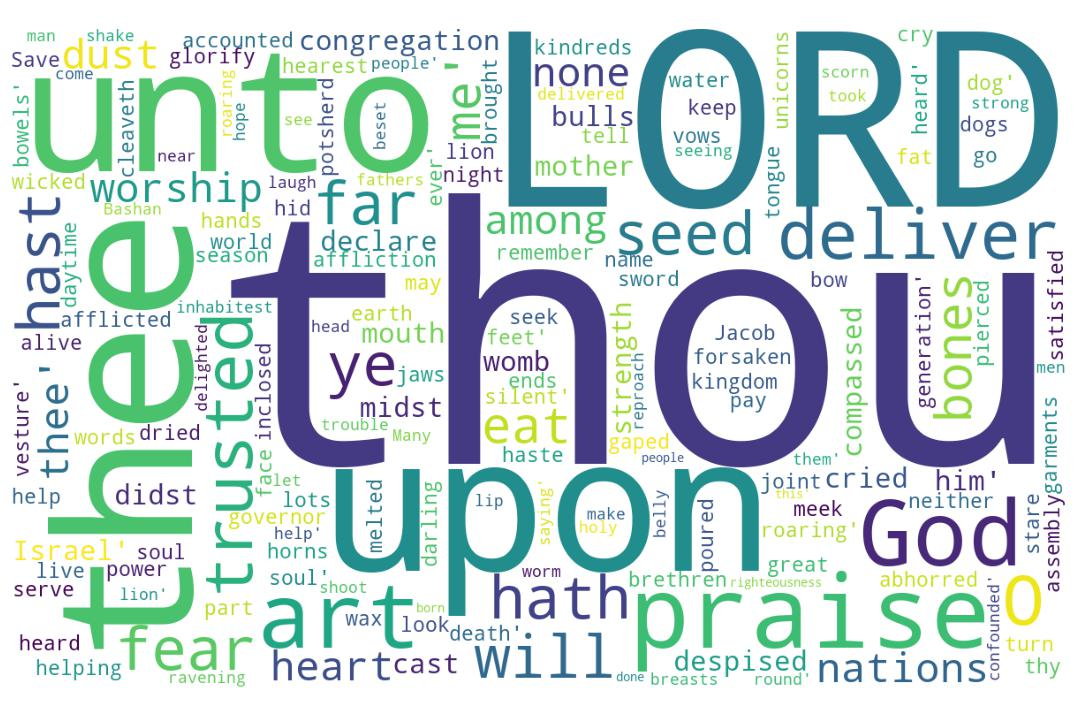
\includegraphics[width=\linewidth]{19OT-Psalms/Psalm22-WordCloud.jpg}
  \caption{Psalm 22 Word Cloud}
  \label{fig:Psalm 22 word Cloud}
\end{figure}

\marginpar{\scriptsize \centering \fcolorbox{bone}{lime}{\textbf{NOW COMES JESUS}}\\ (Psalm 22:1--31) \begin{compactenum}[I.][8]
    \item \textbf{Words of God's Roaring} \index[scripture]{Psalms!Psa 022:01} (Psa 22:1)
    \item The \textbf{Wounds of Suffering} 
    \item The \textbf{Worm of Sin} \index[scripture]{Psalms!Psa 022:06} (Psa  22:6)
    \item The \textbf{Womb of a Servant} \index[scripture]{Psalms!Psa 022:09--10} (Psal 22:9--10)
    \item The \textbf{Wicked that Encompassed him} \index[scripture]{Psalms!Psa 022:12}\index[scripture]{Psalms!Psa 022:16} (Psa 22:12, 16)
    \item The \textbf{World that will Remember} \index[scripture]{Psalms!Psa 022:27} (Psa 22:27)
    \item The \textbf{Ones who will Come} \index[scripture]{Psalms!Psa 022:30}\index[scripture]{Psalms!Psa 022:31} (Psa 22:30, 31)
\end{compactenum}}

\marginpar{\scriptsize \centering \fcolorbox{bone}{yellow}{\textbf{SEVEN LOOKS}}\\ (Psalm 22:1--31) \begin{compactenum}[I.][8]
    \item The \textbf{Upward Look} \index[scripture]{Psalms!Psa 022:01-03} (Psa 22:1--3) 
    \item The \textbf{Backward Look} \index[scripture]{Psalms!Psa 022:04-06} (Psa 22:4--6) 
    \item The \textbf{Outward Look} \index[scripture]{Psalms!Psa 022:07-08} (Psa 22:7--8) 
    \item The \textbf{Inward Look} \index[scripture]{Psalms!Psa 022:14-17} (Psa 22:14--17) 
    \item The \textbf{Downward Look} \index[scripture]{Psalms!Psa 022:18} (Psa 22:18) 
    \item The \textbf{Onward Look} \index[scripture]{Psalms!Psa 022:22} (Psa 22:22) 
    \item The \textbf{Millennial Look} %(Psalm) 
\end{compactenum}}

\marginpar{\scriptsize \centering \fcolorbox{bone}{black}{\textbf{\textcolor[cmyk]{0,0,0,0}{THE WORK ON THE CROSS}}}\\ (Psalm 22:1--31) 
\begin{compactenum}[I.][8]
    \item The \textbf{Separation}  \index[scripture]{Psalms!Psa 022:01}(Psa 22:1) 
    \item The \textbf{Sin} \index[scripture]{Psalms!Psa 022:06}(Psa 22:6)
    \item The \textbf{Scorn} \index[scripture]{Psalms!Psa 022:07}(Psa 22:7)
    \item The \textbf{Strength} \index[scripture]{Psalms!Psa 022:15}(Psa 22:15) 
    \item The \textbf{Season} 
    \item The \textbf{Speech} \index[scripture]{Psalms!Psa 022:22}(Psa 22:22) 
    \item The \textbf{Satisfaction} \index[scripture]{Psalms!Psa 022:26}(Psa 22:26) 
    \item The \textbf{Seed} \index[scripture]{Psalms!Psa 022:30}\index[scripture]{Psalms!Psa 022:31}(Psa 22:30, 31) 
\end{compactenum}}

\marginpar{\scriptsize \centering \fcolorbox{bone}{blue}{\textbf{\textcolor[cmyk]{0,0,0,0}{THE SALVATION NARRATIVE}}}\\ (Psalm 22:1--31) 
\begin{compactenum}[I.][8]
    \item \textbf{Cry of Separation} - (Psa 22:1-5)
    \item \textbf{Cost of Sin} - (Psa 22: 6)  
    \item \textbf{Compassion Seen} - (Psa 22:12, 16)
    \item \textbf{Congregation of the Saints} - (Psa 22: 22, 25)
    \item \textbf{Call of the Saved} - (Psa 22: 23)
    \item \textbf{Concern of the Sovereign} \index[scripture]{Psalms!Psa 022:24} (Psa 22:24)
    \item \textbf{Conclusion of the Story}  - (Psa 22:27-31)
\end{compactenum}}

\marginpar{\scriptsize \centering \fcolorbox{bone}{orange}{\textbf{\textcolor[cmyk]{0,0,0,0}{THE PERSON OF CHRIST}}}\\ (Psalm 22:1--31) \begin{compactenum}[I.][8]
    \item was \textbf{Devoid of God's help} - - completely abandoned by God as he became sin
    \item was on \textbf{Display to the mockers} 
    \item was \textbf{Despised by the people} -- as a fool
    \item was \textbf{Disrobed and naked}  (completed dishonored)
    \item was \textbf{Depleted of energy, emotions, and dignity} 
    \item was \textbf{Distressed and pierced} (Verse 11)
    \item was \textbf{Dying for all sin, past and future} 
\end{compactenum}}

\footnote{\textcolor[cmyk]{0.99998,1,0,0}{\hyperlink{TOC}{Return to end of Table of Contents.}}}\footnote{\href{https://www.audioverse.org/english/audiobibles/books/ENGKJV/O/Ps/1}{\textcolor[cmyk]{0.99998,1,0,0}{Psalms Audio}}}\textcolor[cmyk]{0.99998,1,0,0}{To the chief Musician upon Aijeleth Shahar, A Psalm of David.}\\
\\
\textcolor[cmyk]{0.99998,1,0,0}{My God, my God, why hast thou forsaken me? \emph{why} \emph{art} \emph{thou} \emph{so} far from helping me, \emph{and} \emph{from} the \fcolorbox{bone}{lime}{words of my roaring}?}\footnote{\textbf{Matthew 27:46} - And about the ninth hour Jesus cried with a loud voice, saying, Eli, Eli, lama sabachthani? that is to say, My God, my God, why hast thou forsaken me?}\footnote{\textbf{Mark 15:34} - And at the ninth hour Jesus cried with a loud voice, saying, Eloi, Eloi, lama sabachthani? which is, being interpreted, My God, my God, why hast thou forsaken me?}
[2] \textcolor[cmyk]{0.99998,1,0,0}{O my God, I cry in the daytime, but thou hearest not; and in the night season, and am not silent.}\footnote{\textbf{Psalm 42:3} - My tears have been my meat day and night, while they continually say unto me, Where is thy God?}\footnote{\textbf{Psalm 55:16-17} - As for me, I will call upon God; and the LORD shall save me. [17] Evening, and morning, and at noon, will I pray, and cry aloud: and he shall hear my voice.}\footnote{\textbf{Psalm 88:1} - O LORD God of my salvation, I have cried day and night before thee:}\footnote{\textbf{Luke 18:7} -And shall not God avenge his own elect, which cry day and night unto him, though he bear long with them?}\footnote{\textbf{1 Thessalonians 3:10} - Night and day praying exceedingly that we might see your face, and might perfect that which is lacking in your faith?}\footnote{\textbf{2 Timothy 1:3} - I thank God, whom I serve from my forefathers with pure conscience, that without ceasing I have remembrance of thee in my prayers night and day;}
[3] \textcolor[cmyk]{0.99998,1,0,0}{But thou \emph{art} holy, \emph{O} \emph{thou} that inhabitest the praises of Israel.}\footnote{\textbf{Psalm 145:17} - The LORD is righteous in all his ways, and holy in all his works.}\footnote{\textbf{Isaiah 6:3} - And one cried unto another, and said, Holy, holy, holy, is the LORD of hosts: the whole earth is full of his glory.}\footnote{\textbf{Revelation 4:8} - And the four beasts had each of them six wings about him; and they were full of eyes within: and they rest not day and night, saying, Holy, holy, holy, Lord God Almighty, which was, and is, and is to come.}
[4] \textcolor[cmyk]{0.99998,1,0,0}{Our fathers trusted in thee: they trusted, and thou didst deliver them.}\footnote{\textbf{Genesis 15:6} - And he believed in the LORD; and he counted it to him for righteousness.}
[5] \textcolor[cmyk]{0.99998,1,0,0}{They cried unto thee, and were delivered: they trusted in thee, and were not confounded.}\footnote{\textbf{Psalm 25:2-3} - O my God, I trust in thee: let me not be ashamed, let not mine enemies triumph over me. [3] Yea, let none that wait on thee be ashamed: let them be ashamed which transgress without cause.}\footnote{\textbf{Isaiah 45:17} - But Israel shall be saved in the LORD with an everlasting salvation: ye shall not be ashamed nor confounded world without end.}\footnote{\textbf{1 Peter 2:6} - Wherefore also it is contained in the scripture, Behold, I lay in Sion a chief corner stone, elect, precious: and he that believeth on him shall not be confounded.}
[6] \textcolor[cmyk]{0.99998,1,0,0}{But I \emph{am} \fcolorbox{bone}{lime}{a worm}, and no man; a reproach of men, and despised of the people.}\footnote{\textbf{Job 25:6} - How much less man, that is a worm? and the son of man, which is a worm?}\footnote{\textbf{Isaiah 41:14} - Fear not, thou worm Jacob, and ye men of Israel; I will help thee, saith the LORD, and thy redeemer, the Holy One of Israel.}\footnote{\textbf{Lamentations 3:30} - He giveth his cheek to him that smiteth him: he is filled full with reproach.}
[7] \textcolor[cmyk]{0.99998,1,0,0}{All they that see me laugh me to scorn: they shoot out the lip, they shake the head, \emph{saying},}\footnote{\textbf{Job 16:10} - They have gaped upon me with their mouth; they have smitten me upon the cheek reproachfully; they have gathered themselves together against me.}\footnote{\textbf{Job 30:9-11} - And now am I their song, yea, I am their byword. [10] They abhor me, they flee far from me, and spare not to spit in my face. [11] Because he hath loosed my cord, and afflicted me, they have also let loose the bridle before me.}\footnote{\textbf{Psalm 44:14} - Thou makest us a byword among the heathen, a shaking of the head among the people.}\footnote{\textbf{Psalm 109:25} - I became also a reproach unto them: when they looked upon me they shaked their heads.}\footnote{\textbf{Isaiah 37:22-23} - This is the word which the LORD hath spoken concerning him; The virgin, the daughter of Zion, hath despised thee, and laughed thee to scorn; the daughter of Jerusalem hath shaken her head at thee. [23] Whom hast thou reproached and blasphemed? and against whom hast thou exalted thy voice, and lifted up thine eyes on high? even against the Holy One of Israel.}
[8] \textcolor[cmyk]{0.99998,1,0,0}{He trusted on the LORD \emph{that} he would deliver black{him}: let \fcolorbox{bone}{bone}{him} deliver \fcolorbox{bone}{bone}{him}, seeing he delighted in \fcolorbox{bone}{bone}{him}.}\footnote{\textbf{Psalm 42:10} - As with a sword in my bones, mine enemies reproach me; while they say daily unto me, Where is thy God?}\footnote{\textbf{Isaiah 42:1} - Behold my servant, whom I uphold; mine elect, in whom my soul delighteth; I have put my spirit upon him: he shall bring forth judgment to the Gentiles.}\footnote{\textbf{Matthew 27:42-43} - He saved others; himself he cannot save. If he be the King of Israel, let him now come down from the cross, and we will believe him. [43] He trusted in God; let him deliver him now, if he will have him: for he said, I am the Son of God.}
[9] \textcolor[cmyk]{0.99998,1,0,0}{But thou \emph{art} he that took me out of the \fcolorbox{bone}{lime}{womb}: thou didst make me hope \emph{when} \emph{I} \emph{was} upon my mother's breasts.}\footnote{\textbf{Psalm 7:16} - By thee have I been holden up from the womb: thou art he that took me out of my mother's bowels: my praise shall be continually of thee.}
[10] \textcolor[cmyk]{0.99998,1,0,0}{I was cast upon thee from the womb: thou \emph{art} my God from my mother's belly.}\footnote{\textbf{Isaiah 46:3-4} - Hearken unto me, O house of Jacob, and all the remnant of the house of Israel, which are borne by me from the belly, which are carried from the womb: [4] And even to your old age I am he; and even to hoar hairs will I carry you: I have made, and I will bear; even I will carry, and will deliver you.}
[11] \textcolor[cmyk]{0.99998,1,0,0}{Be not far from me; for trouble \emph{is} near; for \emph{there} \emph{is} none to help.}\footnote{\textbf{Psalm 10:1} - Why standest thou afar off, O LORD? why hidest thou thyself in times of trouble?}\footnote{\textbf{Psalm 13:1-3} - How long wilt thou forget me, O LORD? for ever? how long wilt thou hide thy face from me? [2] How long shall I take counsel in my soul, having sorrow in my heart daily? how long shall mine enemy be exalted over me? [3] Consider and hear me, O LORD my God: lighten mine eyes, lest I sleep the sleep of death;}
[12] \textcolor[cmyk]{0.99998,1,0,0}{Many \fcolorbox{bone}{lime}{bulls} have compassed me: strong \emph{bulls} of Bashan have beset me round.}\footnote{\textbf{Deuteronomy 32:1-15} - Butter of kine, and milk of sheep, with fat of lambs, and rams of the breed of Bashan, and goats, with the fat of kidneys of wheat; and thou didst drink the pure blood of the grape. [15] But Jeshurun waxed fat, and kicked: thou art waxen fat, thou art grown thick, thou art covered with fatness; then he forsook God which made him, and lightly esteemed the Rock of his salvation.}\footnote{\textbf{Ezekiel 39:18} - Ye shall eat the flesh of the mighty, and drink the blood of the princes of the earth, of rams, of lambs, and of goats, of bullocks, all of them fatlings of Bashan.}\footnote{\textbf{Amos 4:1-3} - Hear this word, ye kine of Bashan, that are in the mountain of Samaria, which oppress the poor, which crush the needy, which say to their masters, Bring, and let us drink. [2] The Lord GOD hath sworn by his holiness, that, lo, the days shall come upon you, that he will take you away with hooks, and your posterity with fishhooks. [3] And ye shall go out at the breaches, every cow at that which is before her; and ye shall cast them into the palace, saith the LORD.}
[13] \textcolor[cmyk]{0.99998,1,0,0}{They gaped upon me \emph{with} their mouths, \emph{as} a ravening and a roaring lion.}\footnote{\textbf{Psalm 35:21} - Yea, they opened their mouth wide against me, and said, Aha, aha, our eye hath seen it.}\footnote{\textbf{Job 16:10} - They have gaped upon me with their mouth; they have smitten me upon the cheek reproachfully; they have gathered themselves together against me.}\footnote{\textbf{Lamentations 2:16} - All thine enemies have opened their mouth against thee: they hiss and gnash the teeth: they say, We have swallowed her up: certainly this is the day that we looked for; we have found, we have seen it.}\footnote{\textbf{Lamentations 3:46} - All our enemies have opened their mouths against us.}\footnote{\textbf{1 Peter 5:8} - Be sober, be vigilant; because your adversary the devil, as a roaring lion, walketh about, seeking whom he may devour:}
[14] \textcolor[cmyk]{0.99998,1,0,0}{I am poured out like water, and all my bones are out of joint: my heart is like wax; it is melted in the midst of my bowels.}
[15] \textcolor[cmyk]{0.99998,1,0,0}{My strength is dried up like a potsherd; and my tongue cleaveth to my jaws; and thou hast brought me into the dust of death.}\footnote{\textbf{Psalm 69:3, 21} - I am weary of my crying: my throat is dried: mine eyes fail while I wait for my God. [21] They gave me also gall for my meat; and in my thirst they gave me vinegar to drink.}\footnote{\textbf{Job 29:10} - The nobles held their peace, and their tongue cleaved to the roof of their mouth.}\footnote{\textbf{Lamentations 4:4} - The tongue of the sucking child cleaveth to the roof of his mouth for thirst: the young children ask bread, and no man breaketh it unto them.}\footnote{\textbf{Job 7:21} - And why dost thou not pardon my transgression, and take away mine iniquity? for now shall I sleep in the dust; and thou shalt seek me in the morning, but I shall not be.}\footnote{\textbf{Job 10:9} -  Remember, I beseech thee, that thou hast made me as the clay; and wilt thou bring me into dust again?}\footnote{\textbf{Job 34:15} - All flesh shall perish together, and man shall turn again unto dust.}
[16] \textcolor[cmyk]{0.99998,1,0,0}{For dogs have compassed me: the assembly of the wicked have inclosed me: they pierced my hands and my feet.}\footnote{\textbf{Zechariah 12:10} - And I will pour upon the house of David, and upon the inhabitants of Jerusalem, the spirit of grace and of supplications: and they shall look upon me whom they have pierced, and they shall mourn for him, as one mourneth for his only son, and shall be in bitterness for him, as one that is in bitterness for his firstborn.}\footnote{\textbf{Matthew 27:35} - And they crucified him, and parted his garments, casting lots: that it might be fulfilled which was spoken by the prophet, They parted my garments among them, and upon my vesture did they cast lots.}
[17] \textcolor[cmyk]{0.99998,1,0,0}{I may tell all my bones: they look \emph{and} stare upon me.}\footnote{\textbf{Psalm 102:3-5} - For my days are consumed like smoke, and my bones are burned as an hearth. [4] My heart is smitten, and withered like grass; so that I forget to eat my bread. [5] By reason of the voice of my groaning my bones cleave to my skin.}\footnote{\textbf{Job 33:21} - His flesh is consumed away, that it cannot be seen; and his bones that were not seen stick out.}\footnote{\textbf{Isaiah 52:14} - As many were astonied at thee; his visage was so marred more than any man, and his form more than the sons of men:}
[18] \textcolor[cmyk]{0.99998,1,0,0}{They part my garments among them, and cast lots upon my vesture.}\footnote{\textbf{Matthew 27:35} - And they crucified him, and parted his garments, casting lots: that it might be fulfilled which was spoken by the prophet, They parted my garments among them, and upon my vesture did they cast lots.}\footnote{\textbf{Mark 15:24} - And when they had crucified him, they parted his garments, casting lots upon them, what every man should take.}\footnote{\textbf{Luke 23:34} - Then said Jesus, Father, forgive them; for they know not what they do. And they parted his raiment, and cast lots.}\footnote{\textbf{John 19:23-24} - Then the soldiers, when they had crucified Jesus, took his garments, and made four parts, to every soldier a part; and also his coat: now the coat was without seam, woven from the top throughout. [24] They said therefore among themselves, Let us not rend it, but cast lots for it, whose it shall be: that the scripture might be fulfilled, which saith, They parted my raiment among them, and for my vesture they did cast lots. These things therefore the soldiers did.}
[19] \textcolor[cmyk]{0.99998,1,0,0}{But be not thou far from me, O LORD: O my strength, haste thee to help me.}\footnote{\textbf{Psalm 18:1} - I will love thee, O LORD, my strength.}\footnote{\textbf{Psalm 21:1} - The king shall joy in thy strength, O LORD; and in thy salvation how greatly shall he rejoice!}\footnote{\textbf{Psalm 40:17} - But I am poor and needy; yet the Lord thinketh upon me: thou art my help and my deliverer; make no tarrying, O my God.}
[20] \textcolor[cmyk]{0.99998,1,0,0}{Deliver my soul from the sword; my darling from the power of the dog.}\footnote{\textbf{Psalm 17:13} - Arise, O LORD, disappoint him, cast him down: deliver my soul from the wicked, which is thy sword:}\footnote{\textbf{Zechariah 13:7} - Awake, O sword, against my shepherd, and against the man that is my fellow, saith the LORD of hosts: smite the shepherd, and the sheep shall be scattered: and I will turn mine hand upon the little ones.}\footnote{\textbf{Psalm 35:17} - Lord, how long wilt thou look on? rescue my soul from their destructions, my darling from the lions.}
[21] \textcolor[cmyk]{0.99998,1,0,0}{Save me from the lion's mouth: for thou hast heard me from the horns of the unicorns.}\footnote{\textbf{Numbers 23:22} - God brought them out of Egypt; he hath as it were the strength of an unicorn.}\footnote{\textbf{Deuteronomy 33:17} - His glory is like the firstling of his bullock, and his horns are like the horns of unicorns: with them he shall push the people together to the ends of the earth: and they are the ten thousands of Ephraim, and they are the thousands of Manasseh.}
[22] \textcolor[cmyk]{0.99998,1,0,0}{I will declare thy name unto my brethren: in the midst of the congregation will praise thee.}\footnote{\textbf{Psalm 40:9-10} - I have preached righteousness in the great congregation: lo, I have not refrained my lips, O LORD, thou knowest. [10] I have not hid thy righteousness within my heart; I have declared thy faithfulness and thy salvation: I have not concealed thy lovingkindness and thy truth from the great congregation.}
[23] \textcolor[cmyk]{0.99998,1,0,0}{Ye that fear the LORD, praise \fcolorbox{bone}{bone}{him}; all ye the seed of Jacob, glorify \fcolorbox{bone}{bone}{him}; and fear \fcolorbox{bone}{bone}{him}, all ye the seed of Israel.}\footnote{\textbf{Psalm 115:11} - Ye that fear the LORD, trust in the LORD: he is their help and their shield.}
[24] \textcolor[cmyk]{0.99998,1,0,0}{For he hath not despised nor abhorred the affliction of the afflicted; neither hath he hid his face from \fcolorbox{bone}{bone}{him}; but when he cried unto \fcolorbox{bone}{bone}{him}, he heard.}\footnote{\textbf{Isaiah 50:6-9} - I gave my back to the smiters, and my cheeks to them that plucked off the hair: I hid not my face from shame and spitting. [7] For the Lord GOD will help me; therefore shall I not be confounded: therefore have I set my face like a flint, and I know that I shall not be ashamed. [8] He is near that justifieth me; who will contend with me? let us stand together: who is mine adversary? let him come near to me. [9] Behold, the Lord GOD will help me; who is he that shall condemn me? lo, they all shall wax old as a garment; the moth shall eat them up.}
[25] \textcolor[cmyk]{0.99998,1,0,0}{My praise \emph{shall} \emph{be} of thee in the great congregation: I will pay my vows before them that fear \fcolorbox{bone}{bone}{him}.}\footnote{\textbf{Psalm 56:12} - Thy vows are upon me, O God: I will render praises unto thee.}\footnote{\textbf{Psalm 65:1} - Praise waiteth for thee, O God, in Sion: and unto thee shall the vow be performed.}\footnote{\textbf{Psalm 66:13, 16} - I will go into thy house with burnt offerings: I will pay thee my vows, [16] Come and hear, all ye that fear God, and I will declare what he hath done for my soul.}\footnote{\textbf{Ecclesiastes 5:4-5} - When thou vowest a vow unto God, defer not to pay it; for he hath no pleasure in fools: pay that which thou hast vowed. [5] Better is it that thou shouldest not vow, than that thou shouldest vow and not pay.}\footnote{\textbf{1 Kings 8:65} - And at that time Solomon held a feast, and all Israel with him, a great congregation, from the entering in of Hamath unto the river of Egypt, before the LORD our God, seven days and seven days, even fourteen days.}\footnote{\textbf{2 Chronicles 7:8} - Also at the same time Solomon kept the feast seven days, and all Israel with him, a very great congregation, from the entering in of Hamath unto the river of Egypt.}\footnote{\textbf{2 Choronciles 30:13} - And there assembled at Jerusalem much people to keep the feast of unleavened bread in the second month, a very great congregation.}\footnote{\textbf{Ezra 10:1} - Now when Ezra had prayed, and when he had confessed, weeping and casting himself down before the house of God, there assembled unto him out of Israel a very great congregation of men and women and children: for the people wept very sore.}
[26] \textcolor[cmyk]{0.99998,1,0,0}{The meek shall eat and be satisfied: they shall praise the LORD that seek \fcolorbox{bone}{bone}{him}: your heart shall live for ever.}\footnote{\textbf{Psalm 69:32} - The humble shall see this, and be glad: and your heart shall live that seek God.}
[27] \textcolor[cmyk]{0.99998,1,0,0}{All the ends of the \fcolorbox{bone}{lime}{world} shall remember and turn unto the LORD: and all the kindreds of the nations shall worship before thee.}\footnote{\textbf{Acts 14:15} - And saying, Sirs, why do ye these things? We also are men of like passions with you, and preach unto you that ye should turn from these vanities unto the living God, which made heaven, and earth, and the sea, and all things that are therein:}\footnote{\textbf{Acts 20:21} - Testifying both to the Jews, and also to the Greeks, repentance toward God, and faith toward our Lord Jesus Christ.}\footnote{\textbf{Acts 26:18-20} - To open their eyes, and to turn them from darkness to light, and from the power of Satan unto God, that they may receive forgiveness of sins, and inheritance among them which are sanctified by faith that is in me. [19] Whereupon, O king Agrippa, I was not disobedient unto the heavenly vision: [20] But shewed first unto them of Damascus, and at Jerusalem, and throughout all the coasts of Judaea, and then to the Gentiles, that they should repent and turn to God, and do works meet for repentance.}\footnote{\textbf{1 Thessalonians 1:9} - For they themselves shew of us what manner of entering in we had unto you, and how ye turned to God from idols to serve the living and true God;}
[28] \textcolor[cmyk]{0.99998,1,0,0}{For the kingdom \emph{is} the LORD'S: and he \emph{is} the governor among the nations.}\footnote{\textbf{Psalm 47:7-8} - For God is the King of all the earth: sing ye praises with understanding. [8] God reigneth over the heathen: God sitteth upon the throne of his holiness.}\footnote{\textbf{Daniel 7:14} -And there was given him dominion, and glory, and a kingdom, that all people, nations, and languages, should serve him: his dominion is an everlasting dominion, which shall not pass away, and his kingdom that which shall not be destroyed.}\footnote{\textbf{Obadiah 1:21} - And saviours shall come up on mount Zion to judge the mount of Esau; and the kingdom shall be the LORD'S.}\footnote{\textbf{Zechariah 14:9} - And the LORD shall be king over all the earth: in that day shall there be one LORD, and his name one.}\footnote{\textbf{Matthew 6:13} - And lead us not into temptation, but deliver us from evil: For thine is the kingdom, and the power, and the glory, for ever. Amen.}\footnote{\textbf{Revelation 11:15} - And the seventh angel sounded; and there were great voices in heaven, saying, The kingdoms of this world are become the kingdoms of our Lord, and of his Christ; and he shall reign for ever and ever.}
[29] \textcolor[cmyk]{0.99998,1,0,0}{All \emph{they} \emph{that} \emph{be} fat upon earth shall eat and worship: all they that go down to the dust shall bow before \fcolorbox{bone}{bone}{him}: and none can keep alive his own soul.}
[30] \textcolor[cmyk]{0.99998,1,0,0}{A seed shall serve \fcolorbox{bone}{bone}{him}; it shall be \fcolorbox{bone}{lime}{accounted} to the Lord for a generation.}\footnote{\textbf{1 Peter 2:9} - But ye are a chosen generation, a royal priesthood, an holy nation, a peculiar people; that ye should shew forth the praises of him who hath called you out of darkness into his marvellous light:}
[31] \textcolor[cmyk]{0.99998,1,0,0}{They shall come, and shall declare his righteousness unto a people that shall be born, that he hath done \emph{this}.}


\section{Psalm 22 Comments}

\subsection{Numeric Nuggets}
Psalm 22 is the 500$^{th}$ chapter in the Bible. The word ``him'' is used 13 times in the chapter.

\subsection{Psalm 22:3}
God also is said to inhabit eternity in Isaiah 57:15.\footnote{\textbf{Isaiah 57:15} - For thus saith the high and lofty One that inhabiteth eternity, whose name is Holy; I dwell in the high and holy place, with him also that is of a contrite and humble spirit, to revive the spirit of the humble, and to revive the heart of the contrite ones.}

\subsection{Psalm 22:22}
This is further called ``the great congregation'' in verse 25. This ``great congregation'' first shows up in 1 Kings 8:65, at the dedication of Solomon's Temple.


%\input{19OT-Psalms/Psalm22WordIndex}
\section{Psalm 22 Outlines}

\subsection{My Outlines}

\subsubsection{Now Comes Jesus}
\index[speaker]{Keith Anthony!Psalm 022 (Now Comes Jesus)}
\index[series]{Psalms (Keith Anthony)!Psalm 022 (Now Comes Jesus)}
\index[date]{2014/11/22!Psalm 022 (Now Comes Jesus) (Keith Anthony)}
\textbf{Introduction: }Psalm 22 depicts the first advent of Jesus and his role as the rejected prophet and lamb of God. Consider the parts of that story:
\begin{compactenum}[I.][8]
    \item \textbf{Words of God's Roaring} \index[scripture]{Psalms!Psa 022:01} (Psa 22:1)
    \item The \textbf{Wounds of Suffering} 
    \item The \textbf{Worm of Sin} \index[scripture]{Psalms!Psa 022:06} (Psa 22:6)
    \item The \textbf{Womb of a Servant} \index[scripture]{Psalms!Psa 022:09--10} (Psa 22:9--10)
    \item The \textbf{Wicked that Encompassed Him}  \index[scripture]{Psalms!Psa 022:12}\index[scripture]{Psalms!Psa 022:16} (Psa 22:12, 16)
    \item The \textbf{World that will Remember} \index[scripture]{Psalms!Psa 022:27} (Psa 22:27)
    \item The \textbf{Ones who will Come}  \index[scripture]{Psalms!Psa 022:30}\index[scripture]{Psalms!Psa 022:31} (Psa 22:30, 31)
\end{compactenum}

\subsubsection{Seven Looks from the Cross}
\index[speaker]{Keith Anthony!Psalm 022 (Seven Looks from the Cross)}
\index[series]{Psalms (Keith Anthony)!Psalm 022 (Seven Looks from the Cross)}
\index[date]{Keith Anthony!Psalm 022 (Seven Looks from the Cross) (Keith Anthony)}
%Different Looks:\footnote{05 January 2015}
\begin{compactenum}[I.][8]
    \item The \textbf{Upward Look} (Psa 22:1--3) 
    \item The \textbf{Backward Look} (Psa 22:4--6) 
    \item The \textbf{Outward Look} (Psa 22:7--8) 
    \item The \textbf{Inward Look} (Psa 22:14--17) 
    \item The \textbf{Downward Look} (Psa 22:18) 
    \item The \textbf{Onward Look} (Psa 22:22) 
    \item The \textbf{Millennial Look} %(Psalm) 
\end{compactenum}

\subsubsection{The Work on the Cross}
\index[speaker]{Keith Anthony!Psalm 022 (The Work on the Cross)}
\index[series]{Psalms (Keith Anthony)!Psalm 022 (The Work on the Cross)}
\index[date]{2016/06/27!Psalm 022 (The Work on the Cross) (Keith Anthony)}
%\textbf{Introduction:} Psalm 22 depicts the first advent of Jesus and his role as the rejected prophet and lamb of God. Consider the parts of that story:
\begin{compactenum}[I.][8]
    \item The \textbf{Separation}  \index[scripture]{Psalms!Psa 022:01}(Psa 22:1) 
    \item The \textbf{Sin} \index[scripture]{Psalms!Psa 022:06}(Psa 22:6)
    \item The \textbf{Scorn} \index[scripture]{Psalms!Psa 022:07}(Psa 22:7)
    \item The \textbf{Strength}  \index[scripture]{Psalms!Psa 022:15}(Psa 22:15) 
    \item The \textbf{Season} 
    \item The \textbf{Speech}  \index[scripture]{Psalms!Psa 022:22}(Psa 22:22) 
    \item The \textbf{Satisfaction}  \index[scripture]{Psalms!Psa 022:26}(Psa 22:26) 
    \item The \textbf{Seed}  \index[scripture]{Psalms!Psa 022:30}\index[scripture]{Psalms!Psa 022:31}(Psa 22:30, 31) 
\end{compactenum}

\subsubsection{The Salvation Narrative}
\index[speaker]{Keith Anthony!Psalm 022 (The Salvation Narrative)}
\index[series]{Psalms (Keith Anthony)!Psalm 022 (The Salvation Narrative)}
\index[date]{2014/11/24!Psalm 022 (The Salvation Narrative) (Keith Anthony)}
\textbf{Introduction: }Psalm 22 depicts the first Seen another way, Psalm 22 depicts the parts and purpose of the first advent. Consider the parts of that story:
\begin{compactenum}[I.][8]
    \item The \textbf{Cry of Separation} - (Psa 22:1-5)
    \begin{compactenum}[A.]
        \item Separation from God's presence
        \item Separation from God's place
        \item Separation from God's people
        \item Separation from God's performance
        \item Separation from God's preservation
    \end{compactenum}
    \item The \textbf{Cost of Sin} - (Psa 22: 6)  
    \item The \textbf{Compassion Seen} - (Psa 22:12, 16)
    \item The \textbf{Congregation of the Saints} - (Psa 22: 22, 25)
    \item The \textbf{Call of the Saved} - (Psa 22: 23)
    \item The \textbf{Concern of the Sovereign} \index[scripture]{Psalms!Psa 022:24} (Psa 22:24)
    \item The \textbf{Conclusion of the Story}  - (Psa 22:27-31)
\end{compactenum}

\subsubsection{The Person of Christ as Prophet}
\index[speaker]{Keith Anthony!Psalm 022 (The Person of Christ as Prophet)}
\index[series]{Psalms (Keith Anthony)!Psalm 022 (The Person of Christ as Prophet)}
\index[date]{2014/11/03!Psalm 022 (The Person of Christ as Prophet) (Keith Anthony)}
\textbf{Introduction: }Psalm 22 depicts the first Psalm 22 is the first of the trinity of Psalms (22-24) which depict the triune mission of Jesus Christ as Prophet, Priest, and King. No interpretation of Psalm 22 fits better, or more completely, than Christ's experience on the cross, where he:

\begin{compactenum}[I.][8]
    \item was \textbf{Devoid of God's help} - - completely abandoned by God as he became sin
    \item was on \textbf{Display to the mockers} 
    \item was \textbf{Despised by the people} -- as a fool
    \item was \textbf{Disrobed and naked}  (completed dishonored)
    \item was \textbf{Depleted of energy, emotions, and dignity} 
    \item was \textbf{Distressed and pierced} (Verse 11)
    \item was \textbf{Dying for all sin, past and future} 
\end{compactenum}

\subsection{Outlines from Others}


%\section{Psalm 22 Statistics}

%%%%%%%%%%%%%%%%%%%%%%%%%%%
%%%%% Word Statistics
%%%%%%%%%%%%%%%%%%%%%%%%%%


\normalsize



\subsection{Chapter Word Statistics}


%%%%%%%%%%
%%%%%%%%%%
 
\begin{center}
\begin{longtable}{l|c|c|c|c}
\caption[Stats for Psalm 22]{Stats for Psalm 22} \label{table:Stats for Psalm 22} \\ 
\hline \multicolumn{1}{|c|}{\textbf{Verse(s)}} & \multicolumn{1}{|c|}{\textbf{Count}} & \multicolumn{1}{|c|}{\textbf{Unique}} & \multicolumn{1}{|c|}{\textbf{Italics}} & \multicolumn{1}{|c|}{\textbf{Uniq Italic}}  \\ \hline 
\endfirsthead
 
\multicolumn{5}{c}
{{\bfseries \tablename\ \thetable{} -- continued from previous page}} \\  
\hline \multicolumn{1}{|c|}{\textbf{Verse(s)}} & \multicolumn{1}{|c|}{\textbf{Count}} & \multicolumn{1}{|c|}{\textbf{Unique}} & \multicolumn{1}{|c|}{\textbf{Italics}} & \multicolumn{1}{|c|}{\textbf{Uniq Italic}}  \\ \hline 
\endhead
 
\hline \multicolumn{5}{|r|}{{Continued if needed}} \\ \hline
\endfoot 
1 & 24 & 21 & 6 & 6\\ \hline
2 & 21 & 17 & 0 & 0\\ \hline
3 & 12 & 12 & 3 & 3\\ \hline
4 & 12 & 11 & 0 & 0\\ \hline
5 & 15 & 12 & 0 & 0\\ \hline
6 & 17 & 14 & 1 & 1\\ \hline
7 & 19 & 15 & 1 & 1\\ \hline
8 & 19 & 14 & 1 & 1\\ \hline
9 & 23 & 21 & 4 & 4\\ \hline
10 & 16 & 14 & 1 & 1\\ \hline
11 & 15 & 13 & 3 & 2\\ \hline
12 & 13 & 11 & 1 & 1\\ \hline
13 & 14 & 13 & 2 & 2\\ \hline
14 & 28 & 22 & 0 & 0\\ \hline
15 & 25 & 23 & 0 & 0\\ \hline
16 & 20 & 16 & 0 & 0\\ \hline
17 & 12 & 12 & 1 & 1\\ \hline
18 & 12 & 11 & 0 & 0\\ \hline
19 & 17 & 15 & 0 & 0\\ \hline
20 & 14 & 10 & 0 & 0\\ \hline
21 & 17 & 13 & 0 & 0\\ \hline
22 & 18 & 15 & 0 & 0\\ \hline
23 & 24 & 15 & 0 & 0\\ \hline
24 & 28 & 22 & 0 & 0\\ \hline
25 & 20 & 20 & 2 & 2\\ \hline
26 & 21 & 19 & 0 & 0\\ \hline
27 & 24 & 17 & 0 & 0\\ \hline
28 & 14 & 10 & 2 & 1\\ \hline
29 & 31 & 29 & 3 & 3\\ \hline
30 & 15 & 14 & 0 & 0\\ \hline
31 & 20 & 17 & 1 & 1\\ \hline
\hline \hline
Total & 580 & 246 & 32 & 22



\end{longtable}
\end{center}

%%%%%%%%%%
%%%%%%%%%%
 
\subsection{Words by Frequency}

\begin{center}
\begin{longtable}{l|r}
\caption[Word Frequencies in Psalm 22]{Word Frequencies in Psalm 22} \label{table:WordsIn-Psalm-22} \\ 
\hline \multicolumn{1}{|c|}{\textbf{Word}} & \multicolumn{1}{c|}{\textbf{Frequency}} \\ \hline 
\endfirsthead
 
\multicolumn{2}{c}
{{\bfseries \tablename\ \thetable{} -- continued from previous page}} \\ 
\hline \multicolumn{1}{|c|}{\textbf{Word}} & \multicolumn{1}{c|}{\textbf{Frequency}} \\ \hline 
\endhead
 
\hline \multicolumn{2}{|r|}{{Continued if needed}} \\ \hline
\endfoot
 
\hline \hline
\endlastfoot
the & 40 \\ \hline
my & 21 \\ \hline
and & 21 \\ \hline
of & 19 \\ \hline
me & 18 \\ \hline
him & 13 \\ \hline
shall & 12 \\ \hline
thou & 10 \\ \hline
from & 10 \\ \hline
that & 9 \\ \hline
they & 9 \\ \hline
he & 9 \\ \hline
I & 8 \\ \hline
in & 8 \\ \hline
thee & 8 \\ \hline
a & 7 \\ \hline
not & 6 \\ \hline
to & 6 \\ \hline
upon & 6 \\ \hline
all & 6 \\ \hline
unto & 5 \\ \hline
LORD & 5 \\ \hline
for & 5 \\ \hline
God & 4 \\ \hline
\emph{art} & 4 \\ \hline
But & 4 \\ \hline
trusted & 4 \\ \hline
They & 4 \\ \hline
out & 4 \\ \hline
\emph{is} & 4 \\ \hline
have & 4 \\ \hline
be & 4 \\ \hline
praise & 4 \\ \hline
My & 3 \\ \hline
hast & 3 \\ \hline
far & 3 \\ \hline
O & 3 \\ \hline
deliver & 3 \\ \hline
them & 3 \\ \hline
All & 3 \\ \hline
like & 3 \\ \hline
is & 3 \\ \hline
For & 3 \\ \hline
will & 3 \\ \hline
fear & 3 \\ \hline
seed & 3 \\ \hline
hath & 3 \\ \hline
his & 3 \\ \hline
before & 3 \\ \hline
\emph{thou} & 2 \\ \hline
\emph{and} & 2 \\ \hline
roaring & 2 \\ \hline
but & 2 \\ \hline
am & 2 \\ \hline
Israel & 2 \\ \hline
didst & 2 \\ \hline
cried & 2 \\ \hline
were & 2 \\ \hline
despised & 2 \\ \hline
people & 2 \\ \hline
\emph{that} & 2 \\ \hline
womb & 2 \\ \hline
mother's & 2 \\ \hline
cast & 2 \\ \hline
none & 2 \\ \hline
help & 2 \\ \hline
compassed & 2 \\ \hline
bones & 2 \\ \hline
heart & 2 \\ \hline
it & 2 \\ \hline
midst & 2 \\ \hline
strength & 2 \\ \hline
dust & 2 \\ \hline
among & 2 \\ \hline
soul & 2 \\ \hline
heard & 2 \\ \hline
declare & 2 \\ \hline
congregation & 2 \\ \hline
ye & 2 \\ \hline
\emph{be} & 2 \\ \hline
eat & 2 \\ \hline
nations & 2 \\ \hline
worship & 2 \\ \hline
why & 1 \\ \hline
forsaken & 1 \\ \hline
\emph{why} & 1 \\ \hline
\emph{so} & 1 \\ \hline
helping & 1 \\ \hline
\emph{from} & 1 \\ \hline
words & 1 \\ \hline
cry & 1 \\ \hline
daytime & 1 \\ \hline
hearest & 1 \\ \hline
night & 1 \\ \hline
season & 1 \\ \hline
silent & 1 \\ \hline
holy & 1 \\ \hline
\emph{O} & 1 \\ \hline
inhabitest & 1 \\ \hline
praises & 1 \\ \hline
Our & 1 \\ \hline
fathers & 1 \\ \hline
delivered & 1 \\ \hline
confounded & 1 \\ \hline
\emph{am} & 1 \\ \hline
worm & 1 \\ \hline
no & 1 \\ \hline
man & 1 \\ \hline
reproach & 1 \\ \hline
men & 1 \\ \hline
see & 1 \\ \hline
laugh & 1 \\ \hline
scorn & 1 \\ \hline
shoot & 1 \\ \hline
lip & 1 \\ \hline
shake & 1 \\ \hline
head & 1 \\ \hline
\emph{saying} & 1 \\ \hline
He & 1 \\ \hline
on & 1 \\ \hline
would & 1 \\ \hline
let & 1 \\ \hline
seeing & 1 \\ \hline
delighted & 1 \\ \hline
took & 1 \\ \hline
make & 1 \\ \hline
hope & 1 \\ \hline
\emph{when} & 1 \\ \hline
\emph{I} & 1 \\ \hline
\emph{was} & 1 \\ \hline
breasts & 1 \\ \hline
was & 1 \\ \hline
belly & 1 \\ \hline
Be & 1 \\ \hline
trouble & 1 \\ \hline
near & 1 \\ \hline
\emph{there} & 1 \\ \hline
Many & 1 \\ \hline
bulls & 1 \\ \hline
strong & 1 \\ \hline
\emph{bulls} & 1 \\ \hline
Bashan & 1 \\ \hline
beset & 1 \\ \hline
round & 1 \\ \hline
gaped & 1 \\ \hline
\emph{with} & 1 \\ \hline
their & 1 \\ \hline
mouths & 1 \\ \hline
\emph{as} & 1 \\ \hline
ravening & 1 \\ \hline
lion & 1 \\ \hline
poured & 1 \\ \hline
water & 1 \\ \hline
are & 1 \\ \hline
joint & 1 \\ \hline
wax & 1 \\ \hline
melted & 1 \\ \hline
bowels & 1 \\ \hline
dried & 1 \\ \hline
up & 1 \\ \hline
potsherd & 1 \\ \hline
tongue & 1 \\ \hline
cleaveth & 1 \\ \hline
jaws & 1 \\ \hline
brought & 1 \\ \hline
into & 1 \\ \hline
death & 1 \\ \hline
dogs & 1 \\ \hline
assembly & 1 \\ \hline
wicked & 1 \\ \hline
inclosed & 1 \\ \hline
pierced & 1 \\ \hline
hands & 1 \\ \hline
feet & 1 \\ \hline
may & 1 \\ \hline
tell & 1 \\ \hline
look & 1 \\ \hline
stare & 1 \\ \hline
part & 1 \\ \hline
garments & 1 \\ \hline
lots & 1 \\ \hline
vesture & 1 \\ \hline
haste & 1 \\ \hline
Deliver & 1 \\ \hline
sword & 1 \\ \hline
darling & 1 \\ \hline
power & 1 \\ \hline
dog & 1 \\ \hline
Save & 1 \\ \hline
lion's & 1 \\ \hline
mouth & 1 \\ \hline
horns & 1 \\ \hline
unicorns & 1 \\ \hline
thy & 1 \\ \hline
name & 1 \\ \hline
brethren & 1 \\ \hline
Ye & 1 \\ \hline
Jacob & 1 \\ \hline
glorify & 1 \\ \hline
nor & 1 \\ \hline
abhorred & 1 \\ \hline
affliction & 1 \\ \hline
afflicted & 1 \\ \hline
neither & 1 \\ \hline
hid & 1 \\ \hline
face & 1 \\ \hline
when & 1 \\ \hline
\emph{shall} & 1 \\ \hline
great & 1 \\ \hline
pay & 1 \\ \hline
vows & 1 \\ \hline
The & 1 \\ \hline
meek & 1 \\ \hline
satisfied & 1 \\ \hline
seek & 1 \\ \hline
your & 1 \\ \hline
live & 1 \\ \hline
ever & 1 \\ \hline
ends & 1 \\ \hline
world & 1 \\ \hline
remember & 1 \\ \hline
turn & 1 \\ \hline
kindreds & 1 \\ \hline
kingdom & 1 \\ \hline
LORD'S & 1 \\ \hline
governor & 1 \\ \hline
\emph{they} & 1 \\ \hline
fat & 1 \\ \hline
earth & 1 \\ \hline
go & 1 \\ \hline
down & 1 \\ \hline
bow & 1 \\ \hline
can & 1 \\ \hline
keep & 1 \\ \hline
alive & 1 \\ \hline
own & 1 \\ \hline
A & 1 \\ \hline
serve & 1 \\ \hline
accounted & 1 \\ \hline
Lord & 1 \\ \hline
generation & 1 \\ \hline
come & 1 \\ \hline
righteousness & 1 \\ \hline
born & 1 \\ \hline
done & 1 \\ \hline
\emph{this} & 1 \\ \hline
\end{longtable}
\end{center}



\normalsize



\subsection{Words Alphabetically}

\begin{center}
\begin{longtable}{l|r}
\caption[Word Alphabetically in Psalm 22]{Word Alphabetically in Psalm 22} \label{table:WordsIn-Psalm-22} \\ 
\hline \multicolumn{1}{|c|}{\textbf{Word}} & \multicolumn{1}{c|}{\textbf{Frequency}} \\ \hline 
\endfirsthead
 
\multicolumn{2}{c}
{{\bfseries \tablename\ \thetable{} -- continued from previous page}} \\ 
\hline \multicolumn{1}{|c|}{\textbf{Word}} & \multicolumn{1}{c|}{\textbf{Frequency}} \\ \hline 
\endhead
 
\hline \multicolumn{2}{|r|}{{Continued if needed}} \\ \hline
\endfoot
 
\hline \hline
\endlastfoot
A & 1 \\ \hline
All & 3 \\ \hline
Bashan & 1 \\ \hline
Be & 1 \\ \hline
But & 4 \\ \hline
Deliver & 1 \\ \hline
For & 3 \\ \hline
God & 4 \\ \hline
He & 1 \\ \hline
I & 8 \\ \hline
Israel & 2 \\ \hline
Jacob & 1 \\ \hline
LORD & 5 \\ \hline
LORD'S & 1 \\ \hline
Lord & 1 \\ \hline
Many & 1 \\ \hline
My & 3 \\ \hline
O & 3 \\ \hline
Our & 1 \\ \hline
Save & 1 \\ \hline
The & 1 \\ \hline
They & 4 \\ \hline
Ye & 1 \\ \hline
\emph{I} & 1 \\ \hline
\emph{O} & 1 \\ \hline
\emph{am} & 1 \\ \hline
\emph{and} & 2 \\ \hline
\emph{art} & 4 \\ \hline
\emph{as} & 1 \\ \hline
\emph{be} & 2 \\ \hline
\emph{bulls} & 1 \\ \hline
\emph{from} & 1 \\ \hline
\emph{is} & 4 \\ \hline
\emph{saying} & 1 \\ \hline
\emph{shall} & 1 \\ \hline
\emph{so} & 1 \\ \hline
\emph{that} & 2 \\ \hline
\emph{there} & 1 \\ \hline
\emph{they} & 1 \\ \hline
\emph{this} & 1 \\ \hline
\emph{thou} & 2 \\ \hline
\emph{was} & 1 \\ \hline
\emph{when} & 1 \\ \hline
\emph{why} & 1 \\ \hline
\emph{with} & 1 \\ \hline
a & 7 \\ \hline
abhorred & 1 \\ \hline
accounted & 1 \\ \hline
afflicted & 1 \\ \hline
affliction & 1 \\ \hline
alive & 1 \\ \hline
all & 6 \\ \hline
am & 2 \\ \hline
among & 2 \\ \hline
and & 21 \\ \hline
are & 1 \\ \hline
assembly & 1 \\ \hline
be & 4 \\ \hline
before & 3 \\ \hline
belly & 1 \\ \hline
beset & 1 \\ \hline
bones & 2 \\ \hline
born & 1 \\ \hline
bow & 1 \\ \hline
bowels & 1 \\ \hline
breasts & 1 \\ \hline
brethren & 1 \\ \hline
brought & 1 \\ \hline
bulls & 1 \\ \hline
but & 2 \\ \hline
can & 1 \\ \hline
cast & 2 \\ \hline
cleaveth & 1 \\ \hline
come & 1 \\ \hline
compassed & 2 \\ \hline
confounded & 1 \\ \hline
congregation & 2 \\ \hline
cried & 2 \\ \hline
cry & 1 \\ \hline
darling & 1 \\ \hline
daytime & 1 \\ \hline
death & 1 \\ \hline
declare & 2 \\ \hline
delighted & 1 \\ \hline
deliver & 3 \\ \hline
delivered & 1 \\ \hline
despised & 2 \\ \hline
didst & 2 \\ \hline
dog & 1 \\ \hline
dogs & 1 \\ \hline
done & 1 \\ \hline
down & 1 \\ \hline
dried & 1 \\ \hline
dust & 2 \\ \hline
earth & 1 \\ \hline
eat & 2 \\ \hline
ends & 1 \\ \hline
ever & 1 \\ \hline
face & 1 \\ \hline
far & 3 \\ \hline
fat & 1 \\ \hline
fathers & 1 \\ \hline
fear & 3 \\ \hline
feet & 1 \\ \hline
for & 5 \\ \hline
forsaken & 1 \\ \hline
from & 10 \\ \hline
gaped & 1 \\ \hline
garments & 1 \\ \hline
generation & 1 \\ \hline
glorify & 1 \\ \hline
go & 1 \\ \hline
governor & 1 \\ \hline
great & 1 \\ \hline
hands & 1 \\ \hline
hast & 3 \\ \hline
haste & 1 \\ \hline
hath & 3 \\ \hline
have & 4 \\ \hline
he & 9 \\ \hline
head & 1 \\ \hline
heard & 2 \\ \hline
hearest & 1 \\ \hline
heart & 2 \\ \hline
help & 2 \\ \hline
helping & 1 \\ \hline
hid & 1 \\ \hline
him & 13 \\ \hline
his & 3 \\ \hline
holy & 1 \\ \hline
hope & 1 \\ \hline
horns & 1 \\ \hline
in & 8 \\ \hline
inclosed & 1 \\ \hline
inhabitest & 1 \\ \hline
into & 1 \\ \hline
is & 3 \\ \hline
it & 2 \\ \hline
jaws & 1 \\ \hline
joint & 1 \\ \hline
keep & 1 \\ \hline
kindreds & 1 \\ \hline
kingdom & 1 \\ \hline
laugh & 1 \\ \hline
let & 1 \\ \hline
like & 3 \\ \hline
lion & 1 \\ \hline
lion's & 1 \\ \hline
lip & 1 \\ \hline
live & 1 \\ \hline
look & 1 \\ \hline
lots & 1 \\ \hline
make & 1 \\ \hline
man & 1 \\ \hline
may & 1 \\ \hline
me & 18 \\ \hline
meek & 1 \\ \hline
melted & 1 \\ \hline
men & 1 \\ \hline
midst & 2 \\ \hline
mother's & 2 \\ \hline
mouth & 1 \\ \hline
mouths & 1 \\ \hline
my & 21 \\ \hline
name & 1 \\ \hline
nations & 2 \\ \hline
near & 1 \\ \hline
neither & 1 \\ \hline
night & 1 \\ \hline
no & 1 \\ \hline
none & 2 \\ \hline
nor & 1 \\ \hline
not & 6 \\ \hline
of & 19 \\ \hline
on & 1 \\ \hline
out & 4 \\ \hline
own & 1 \\ \hline
part & 1 \\ \hline
pay & 1 \\ \hline
people & 2 \\ \hline
pierced & 1 \\ \hline
potsherd & 1 \\ \hline
poured & 1 \\ \hline
power & 1 \\ \hline
praise & 4 \\ \hline
praises & 1 \\ \hline
ravening & 1 \\ \hline
remember & 1 \\ \hline
reproach & 1 \\ \hline
righteousness & 1 \\ \hline
roaring & 2 \\ \hline
round & 1 \\ \hline
satisfied & 1 \\ \hline
scorn & 1 \\ \hline
season & 1 \\ \hline
see & 1 \\ \hline
seed & 3 \\ \hline
seeing & 1 \\ \hline
seek & 1 \\ \hline
serve & 1 \\ \hline
shake & 1 \\ \hline
shall & 12 \\ \hline
shoot & 1 \\ \hline
silent & 1 \\ \hline
soul & 2 \\ \hline
stare & 1 \\ \hline
strength & 2 \\ \hline
strong & 1 \\ \hline
sword & 1 \\ \hline
tell & 1 \\ \hline
that & 9 \\ \hline
the & 40 \\ \hline
thee & 8 \\ \hline
their & 1 \\ \hline
them & 3 \\ \hline
they & 9 \\ \hline
thou & 10 \\ \hline
thy & 1 \\ \hline
to & 6 \\ \hline
tongue & 1 \\ \hline
took & 1 \\ \hline
trouble & 1 \\ \hline
trusted & 4 \\ \hline
turn & 1 \\ \hline
unicorns & 1 \\ \hline
unto & 5 \\ \hline
up & 1 \\ \hline
upon & 6 \\ \hline
vesture & 1 \\ \hline
vows & 1 \\ \hline
was & 1 \\ \hline
water & 1 \\ \hline
wax & 1 \\ \hline
were & 2 \\ \hline
when & 1 \\ \hline
why & 1 \\ \hline
wicked & 1 \\ \hline
will & 3 \\ \hline
womb & 2 \\ \hline
words & 1 \\ \hline
world & 1 \\ \hline
worm & 1 \\ \hline
worship & 2 \\ \hline
would & 1 \\ \hline
ye & 2 \\ \hline
your & 1 \\ \hline
\end{longtable}
\end{center}



\normalsize



\subsection{Word Lengths in Chapter}
\normalsize
\begin{longtable}{l|p{3.75in}}
\caption[Words by Length in Psalm 22]{Words by Length in Psalm 22} \label{table:WordsIn-Psalm-22} \\ 
\hline \multicolumn{1}{|c|}{\textbf{Length}} & \multicolumn{1}{c|}{\textbf{Words}} \\ \hline 
\endfirsthead
 
\multicolumn{2}{c}
{{\bfseries \tablename\ \thetable{} -- continued from previous page}} \\ 
\hline \multicolumn{1}{|c|}{\textbf{Length}} & \multicolumn{1}{c|}{\textbf{Words}} \\ \hline 
\endhead
 
\hline \multicolumn{2}{|r|}{{Continued if needed}} \\ \hline
\endfoot
 
\hline \hline
\endlastfoot
1 & O, I, \emph{O}, a, \emph{I}, A \\ \hline
2 & My, my, me, \emph{so}, of, in, am, \emph{am}, no, to, He, on, he, Be, \emph{is}, \emph{as}, is, it, up, be, Ye, ye, \emph{be}, go \\ \hline
3 & God, why, \emph{why}, \emph{art}, far, \emph{and}, the, cry, but, not, and, But, Our, man, men, All, see, out, lip, him, let, \emph{was}, was, for, all, are, wax, For, may, dog, thy, nor, hid, his, pay, The, eat, fat, bow, can, own \\ \hline
4 & hast, thou, \emph{thou}, from, \emph{from}, holy, that, thee, they, them, They, unto, were, worm, head, LORD, \emph{that}, took, womb, make, hope, \emph{when}, upon, cast, near, none, help, Many, have, \emph{with}, lion, like, jaws, into, dust, dogs, feet, tell, look, part, lots, soul, Save, will, name, fear, seed, hath, face, when, vows, meek, seek, your, live, ever, ends, turn, \emph{they}, down, keep, Lord, come, born, done, \emph{this} \\ \hline
5 & words, night, didst, cried, laugh, scorn, shoot, shake, would, belly, \emph{there}, bulls, \emph{bulls}, beset, round, gaped, their, water, bones, joint, heart, midst, dried, death, hands, stare, among, haste, sword, power, mouth, heard, horns, Jacob, \emph{shall}, great, shall, world, earth, alive, serve \\ \hline
6 & season, silent, Israel, people, \emph{saying}, seeing, strong, Bashan, mouths, poured, melted, bowels, tongue, wicked, lion's, praise, before, LORD'S \\ \hline
7 & helping, roaring, daytime, hearest, praises, fathers, trusted, deliver, breasts, trouble, brought, pierced, vesture, Deliver, darling, declare, glorify, neither, nations, worship, kingdom \\ \hline
8 & forsaken, reproach, despised, mother's, ravening, strength, potsherd, cleaveth, assembly, inclosed, garments, unicorns, brethren, abhorred, remember, kindreds, governor \\ \hline
9 & delivered, delighted, compassed, afflicted, satisfied, accounted \\ \hline
10 & inhabitest, confounded, affliction, generation \\ \hline
12 & congregation \\ \hline
13 & righteousness \\ \hline
\end{longtable}






%%%%%%%%%%
%%%%%%%%%%
 



%%%%%%%%%%
%%%%%%%%%%
\subsection{Verses with 13 Words in Chapter}
\normalsize
\begin{longtable}{l|p{3.75in}}
\caption[Verses with 13 Words  in Psalm 22]{Verses with 13 Words  in Psalm 22} \label{table:Verses with 13 Words in-Psalm-22} \\ 
\hline \multicolumn{1}{|c|}{\textbf{Reference}} & \multicolumn{1}{c|}{\textbf{Verse}} \\ \hline 
\endfirsthead
 
\multicolumn{2}{c}
{{\bfseries \tablename\ \thetable{} -- continued from previous page}} \\ 
\hline \multicolumn{1}{|c|}{\textbf{Reference}} & \multicolumn{1}{c|}{\textbf{Verse}} \\ \hline 
\endhead
 
\hline \multicolumn{2}{|r|}{{Continued if needed}} \\ \hline
\endfoot
 
\hline \hline
\endlastfoot
Psalms 022:12 & Many bulls have compassed me: strong \emph{bulls} of Bashan have beset me round. \\ \hline
\end{longtable}






%%%%%%%%%%
%%%%%%%%%%
 



%%%%%%%%%%
%%%%%%%%%%
\subsection{Verses with 18 Words in Chapter}
\normalsize
\begin{longtable}{l|p{3.75in}}
\caption[Verses with 18 Words  in Psalm 22]{Verses with 18 Words  in Psalm 22} \label{table:Verses with 18 Words in-Psalm-22} \\ 
\hline \multicolumn{1}{|c|}{\textbf{Reference}} & \multicolumn{1}{c|}{\textbf{Verse}} \\ \hline 
\endfirsthead
 
\multicolumn{2}{c}
{{\bfseries \tablename\ \thetable{} -- continued from previous page}} \\ 
\hline \multicolumn{1}{|c|}{\textbf{Reference}} & \multicolumn{1}{c|}{\textbf{Verse}} \\ \hline 
\endhead
 
\hline \multicolumn{2}{|r|}{{Continued if needed}} \\ \hline
\endfoot
 
\hline \hline
\endlastfoot
Psalms 022:22 & I will declare thy name unto my brethren: in the midst of the congregation will I praise thee. \\ \hline
\end{longtable}






%%%%%%%%%%
%%%%%%%%%%
\subsection{Psalm 22 Repeated Phrases}


%%%%%%%%%%
%%%%%%%%%%
\normalsize
 
\begin{center}
\begin{longtable}{|p{3.0in}|p{0.5in}|}
\caption[Psalm 22 Repeated Phrases]{Psalm 22 Repeated Phrases}\label{table:Repeated Phrases Psalm 22} \\
\hline \multicolumn{1}{|c|}{\textbf{Phrase}} & \multicolumn{1}{c|}{\textbf{Frequency}} \\ \hline 
\endfirsthead
 
\multicolumn{2}{c}
{{\bfseries \tablename\ \thetable{} -- continued from previous page}} \\  
\hline \multicolumn{1}{|c|}{\textbf{Phrase}} & \multicolumn{1}{c|}{\textbf{Frequency}} \\ \hline 
\endhead
 
\hline \multicolumn{2}{c}{{ }} \\ \hline
\endfoot 
of the & 9\\ \hline 
in the & 5\\ \hline 
from the & 5\\ \hline 
the LORD & 4\\ \hline 
my God & 3\\ \hline 
far from & 3\\ \hline 
thou \emph{art} & 3\\ \hline 
\end{longtable}
\end{center}



%%%%%%%%%%
%%%%%%%%%%




\chapter{Psalm 23}

\begin{figure}
  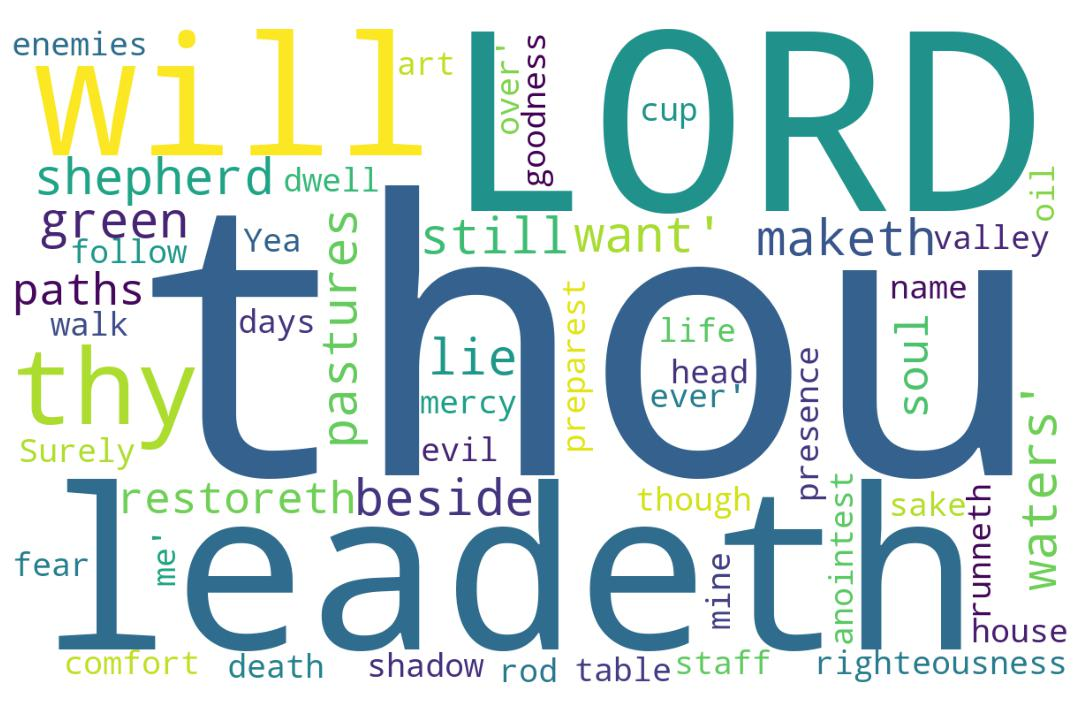
\includegraphics[width=\linewidth]{19OT-Psalms/Psalm23-WordCloud.jpg}
  \caption{Psalm 23 Word Cloud}
  \label{fig:Psalm 23 word Cloud}
\end{figure}

\marginpar{\scriptsize \centering \fcolorbox{bone}{lime}{\textbf{MY SHEPHERD GIVES ME}}\\ (Psalm 23:1--06) \begin{compactenum}[I.][8]
    \item \textbf{Provision} \index[scripture]{Psalms!Psa 023:01}(Psa 23:1)
    \item \textbf{Pastures} \index[scripture]{Psalms!Psa 023:02}(Psa 23:2)
    \item \textbf{Paths} \index[scripture]{Psalms!Psa 023:03}(Psa 23:3)
    \item \textbf{Protection} \index[scripture]{Psalms!Psa 023:04}(Psa 23:4)
    \item \textbf{Presence} \index[scripture]{Psalms!Psa 023:05}(Psa 23:5)
    \item A \textbf{Prepared} Table \index[scripture]{Psalms!Psa 023:05}(Psa 23:5)
    \item \textbf{Preservation} \index[scripture]{Psalms!Psa 023:06}(Psa 23:6)
\end{compactenum}}

\marginpar{\scriptsize \centering \fcolorbox{bone}{yellow}{\textbf{I SHALL NOT WANT}}\\ (Psalm 23:1--06) \begin{compactenum}[I.][8]

    \item \textbf{Still Waters} \index[scripture]{Psalms!Psa 023:02}(Psa 23:2)
    \item \textbf{Serene Pastures} \index[scripture]{Psalms!Psa 023:03}(Psa 23:3)
    \item \textbf{Restored Soul} \index[scripture]{Psalms!Psa 023:03}(Psa 23:3)
    \item \textbf{Supporting Staff} \index[scripture]{Psalms!Psa 023:04}(Psa 23:4)
    \item \textbf{Set Table} \index[scripture]{Psalms!Psa 023:05}(Psa 23:5)
    \item \textbf{Sure Goodness} \index[scripture]{Psalms!Psa 023:06}(Psa 23:6)
    \item \textbf{Certain Mercy} \index[scripture]{Psalms!Psa 023:06}(Psa 23:6)
\end{compactenum}}

\marginpar{\scriptsize \centering \fcolorbox{bone}{black}{\textbf{\textcolor{white}{SHEPHERD IN THE WILDERNESS}}}\\ (Psalm 23:1--06)
%\marginpar{\scriptsize \centering \fcolorbox{bone}{black}{\textbf{\textcolor{white}{SHEPHERD IN THE}\\\fcolorbox{bone}{black}{\textbf{\textcolor{white}{WILDERNESS}}}\\ (Psalm 23:1--06) 
 \begin{compactenum}[I.][8]
    \item The \textbf{Ruggedness} %\index[scripture]{Psalms!Psa 023:02}(Psa 23:2)
    \item The \textbf{Rocks} %\index[scripture]{Psalms!Psa 023:02}(Psa 23:2)
    \item The \textbf{Route} %\index[scripture]{Psalms!Psa 023:02}(Psa 23:2)
    \item The \textbf{Rain} %\index[scripture]{Psalms!Psa 023:02}(Psa 23:2)
    \item The \textbf{Rod} %\index[scripture]{Psalms!Psa 023:02}(Psa 23:2)
    \item The \textbf{Recognition} %\index[scripture]{Psalms!Psa 023:02}(Psa 23:2)
\end{compactenum}}

%% Wanting, Waters, Walk, War, Wellness
%% residence [6], restoration [3], righteousness [3], running cup [5], the rod [4], rest [2], 

\footnote{\textcolor[cmyk]{0.99998,1,0,0}{\hyperlink{TOC}{Return to end of Table of Contents.}}}\footnote{\href{https://audiobible.com/bible}{\textcolor[cmyk]{0.99998,1,0,0}{Psalm 23 Audio}}}\textcolor[cmyk]{0.99998,1,0,0}{The LORD \emph{is} my shepherd; I \fcolorbox{bone}{lime}{shall not want}.}
[2] \textcolor[cmyk]{0.99998,1,0,0}{He maketh me to lie down in green \fcolorbox{bone}{lime}{pastures}: he leadeth me beside the still waters.}
[3] \textcolor[cmyk]{0.99998,1,0,0}{He restoreth my soul: he leadeth me in the \fcolorbox{bone}{lime}{paths} of righteousness for his name's sake.}
[4] \textcolor[cmyk]{0.99998,1,0,0}{Yea, though I walk through the valley of the shadow of death, I will \fcolorbox{bone}{lime}{fear no evil}: for thou \emph{art} with me; thy rod and thy staff they comfort me.}
[5] \textcolor[cmyk]{0.99998,1,0,0}{Thou \fcolorbox{bone}{lime}{preparest} a table before me in the \fcolorbox{bone}{lime}{presence} of mine enemies: thou anointest my head with oil; my cup runneth over.}
[6] \textcolor[cmyk]{0.99998,1,0,0}{Surely goodness and mercy shall follow me all the days of my life: and I will dwell in the house of the LORD \fcolorbox{bone}{lime}{for ever}.}
\section{Psalm 23 Comments}

\subsection{Numeric Nuggets}
\textbf{13:} The 13-letter word ``righteousness'' is used in the chapter.
%\input{19OT-Psalms/Psalm23WordIndex}
\section{Psalm 23 Outlines}

\subsection{My Outlines}

\subsubsection{My Shepherd Gives Me}

\index[speaker]{Keith Anthony!Psalm 023 (My Shepherd Gives Me)}
\index[series]{Psalms (Keith Anthony)!Psalm 023 (My Shepherd Gives Me)}
\index[date]{2016/06/29!Psalm 023 (My Shepherd Gives Me) (Keith Anthony)}

\begin{compactenum}[I.]
    \item \textbf{Provision} \index[scripture]{Psalms!Psa 023:01}(Psa 23:1)
    \item \textbf{Pastures} \index[scripture]{Psalms!Psa 023:02}(Psa 23:2)
    \item \textbf{Paths} \index[scripture]{Psalms!Psa 023:03}(Psa 23:3)
    \item \textbf{Protection} \index[scripture]{Psalms!Psa 023:04}(Psa 23:4)
    \item \textbf{Presence} \index[scripture]{Psalms!Psa 023:05}(Psa 23:5)
    \item A \textbf{Prepared} Table \index[scripture]{Psalms!Psa 023:05}(Psa 23:5)
    \item \textbf{Preservation} \index[scripture]{Psalms!Psa 023:06}(Psa 23:6)
\end{compactenum}

\subsubsection{I Shall Not Want}

\index[speaker]{Keith Anthony!Psalm 023 (I Shall Not Want)}
\index[series]{Psalms (Keith Anthony)!Psalm 023 (I Shall Not Want)}
\index[date]{2018/0520/06!Psalm 023 (I Shall Not Want) (Keith Anthony)}
\begin{compactenum}[I.]
    \item \textbf{Still Waters} \index[scripture]{Psalms!Psa 023:02}(Psa 23:2)
    \item \textbf{Serene Pastures} \index[scripture]{Psalms!Psa 023:03}(Psa 23:3)
    \item \textbf{Restored Soul} \index[scripture]{Psalms!Psa 023:03}(Psa 23:3)
    \item \textbf{Supporting Staff} \index[scripture]{Psalms!Psa 023:04}(Psa 23:4)
    \item \textbf{Set Table} \index[scripture]{Psalms!Psa 023:05}(Psa 23:5)
    \item \textbf{Sure Goodness} \index[scripture]{Psalms!Psa 023:06}(Psa 23:6)
    \item \textbf{Certain Mercy} \index[scripture]{Psalms!Psa 023:06}(Psa 23:6)
\end{compactenum}


\subsubsection{The Shepherd in the Wilderness}

\index[speaker]{Keith Anthony!Psalm 023 (The Shepherd in the Wilderness)}
\index[series]{Psalms (Keith Anthony)!Psalm 023 (The Shepherd in the Wilderness)}
\index[date]{2017/08/06!Psalm 023 (The Shepherd in the Wilderness) (Keith Anthony)}

\begin{compactenum}[I.]
    \item The \textbf{Ruggedness} -- rugged wilderness covers much of Israel. The two most prominent deserts are the Judea Wilderness running along the eastern edge of the Judea Mountains, and the Negev lying in southern Israel. Israel's wilderness abounds with rocks, hills, and canyons. The climate is one of extremes swith scorching hot temperatures by day turn to near-freezing temperatures at night. Though it receives little rainfall, the wilderness can sustain the flocks of nomadic shepherds. The Negev desert where David would have grazed his sheep is a far cry from the abundantly grassy meadows of Sunday school paintings. It is a desert after all. From time to time our bus would pass by a hill covered in sparse grass and we would see Bedouin shepherds grazing their flocks on it. Then miles would pass, miles of hills covered in nothing but dust and rock, before another hill would appear which sported the tiny patches of green.
	\item The \textbf{Rocks} -- Westerners imagine lush, green meadows when they hear the word ``pasture,'' but ``green pastures'' in Israel actually look like rocky, barren hillsides. Scattered amidst the rocks are blades of grass. Where a drop of rain fell or dew collected beneath a rock, a single tuft of grass can sprout up. %\index[scripture]{Psalms!Psalm 023:01}(Psalm 23:1)
    \item The \textbf{Route} -- When you look at the hills in the Negev, you see what looks like ``terraces'' on them.  These are the grazing paths where the shepherds have led their flocks.
    \item The \textbf{Rain} -- There hardly ever is rain in the Negev desert. Instead, sometimes a slightly damp breeze blows in from the sea to the west.  From these breezes, moisture condenses on the hills allowing grass to grow.  What about the still waters? As other travelers could tell you, the climate in Israel is typically hot and dry, but my group had the opportunity to visit during the brief rainy season. It rained almost every day, soaking us to the bone and pushing our cheap tourist umbrellas to their limits. During this season, the wadis are suddenly filled with water. A wadi is a stream bed in the desert that is dry all year `round until the rainy season comes. During this season, all the water that falls on the hills is channeled down into the wadis and they burst violently into life, rushing angrily down the hills into the Dead Sea.  If a shepherd led his sheep to drink in a wadi, they would be dragged in and under. They would be carried along by the merciless current and smashed repeatedly against the rocks until their drowned and broken bodies reached the wadi's destination. ``A good shepherd is a shepherd who can find still waters in the midst of a desert, from which his sheep can drink in safety.''
    \item The \textbf{Rod} -- The shepherd has a rod and a staff. These are used mainly to put wayward sheep back on the correct path. The wrong path (1) will not have enough food, and (2) will be a place of predators.
    \item The \textbf{Recognition} -- Over time, sheep in a flock will comes to recognize the voice of their shepherd. Another aspect of recognition is that the shepherd is aware that the sheep he is watching belong to someone else!
\end{compactenum}


\subsection{Outlines from Others}

%\section{Psalm 23 Statistics}

%%%%%%%%%%%%%%%%%%%%%%%%%%%
%%%%%Word Statistics
%%%%%%%%%%%%%%%%%%%%%%%%%%%


\normalsize



\subsection{Chapter Word Statistics}


%%%%%%%%%%
%%%%%%%%%%
 
\begin{center}
\begin{longtable}{l|c|c|c|c}
\caption[Stats for Psalm 23]{Stats for Psalm 23} \label{table:Stats for Psalm 23} \\ 
\hline \multicolumn{1}{|c|}{\textbf{Verse(s)}} & \multicolumn{1}{|c|}{\textbf{Count}} & \multicolumn{1}{|c|}{\textbf{Unique}} & \multicolumn{1}{|c|}{\textbf{Italics}} & \multicolumn{1}{|c|}{\textbf{Uniq Italic}}  \\ \hline 
\endfirsthead
 
\multicolumn{5}{c}
{{\bfseries \tablename\ \thetable{} -- continued from previous page}} \\  
\hline \multicolumn{1}{|c|}{\textbf{Verse(s)}} & \multicolumn{1}{|c|}{\textbf{Count}} & \multicolumn{1}{|c|}{\textbf{Unique}} & \multicolumn{1}{|c|}{\textbf{Italics}} & \multicolumn{1}{|c|}{\textbf{Uniq Italic}}  \\ \hline 
\endhead
 
\hline \multicolumn{5}{|r|}{{Continued if needed}} \\ \hline
\endfoot 
1 & 9 & 9 & 1 & 1\\ \hline
2 & 16 & 15 & 0 & 0\\ \hline
3 & 16 & 16 & 0 & 0\\ \hline
4 & 30 & 25 & 1 & 1\\ \hline
5 & 22 & 21 & 0 & 0\\ \hline
6 & 25 & 21 & 0 & 0\\ \hline
\hline \hline
Total & 118 & 77 & 2 & 2



\end{longtable}
\end{center}

%%%%%%%%%%
%%%%%%%%%%
 
\subsection{Words by Frequency}

\begin{center}
\begin{longtable}{l|r}
\caption[Word Frequencies in Psalm 23]{Word Frequencies in Psalm 23} \label{table:WordsIn-Psalm-23} \\ 
\hline \multicolumn{1}{|c|}{\textbf{Word}} & \multicolumn{1}{c|}{\textbf{Frequency}} \\ \hline 
\endfirsthead
 
\multicolumn{2}{c}
{{\bfseries \tablename\ \thetable{} -- continued from previous page}} \\ 
\hline \multicolumn{1}{|c|}{\textbf{Word}} & \multicolumn{1}{c|}{\textbf{Frequency}} \\ \hline 
\endhead
 
\hline \multicolumn{2}{|r|}{{Continued if needed}} \\ \hline
\endfoot
 
\hline \hline
\endlastfoot
the & 8 \\ \hline
me & 7 \\ \hline
of & 6 \\ \hline
my & 5 \\ \hline
I & 4 \\ \hline
in & 4 \\ \hline
for & 3 \\ \hline
and & 3 \\ \hline
LORD & 2 \\ \hline
shall & 2 \\ \hline
He & 2 \\ \hline
he & 2 \\ \hline
leadeth & 2 \\ \hline
will & 2 \\ \hline
thou & 2 \\ \hline
with & 2 \\ \hline
thy & 2 \\ \hline
The & 1 \\ \hline
\emph{is} & 1 \\ \hline
shepherd & 1 \\ \hline
not & 1 \\ \hline
want & 1 \\ \hline
maketh & 1 \\ \hline
to & 1 \\ \hline
lie & 1 \\ \hline
down & 1 \\ \hline
green & 1 \\ \hline
pastures & 1 \\ \hline
beside & 1 \\ \hline
still & 1 \\ \hline
waters & 1 \\ \hline
restoreth & 1 \\ \hline
soul & 1 \\ \hline
paths & 1 \\ \hline
righteousness & 1 \\ \hline
his & 1 \\ \hline
name's & 1 \\ \hline
sake & 1 \\ \hline
Yea & 1 \\ \hline
though & 1 \\ \hline
walk & 1 \\ \hline
through & 1 \\ \hline
valley & 1 \\ \hline
shadow & 1 \\ \hline
death & 1 \\ \hline
fear & 1 \\ \hline
no & 1 \\ \hline
evil & 1 \\ \hline
\emph{art} & 1 \\ \hline
rod & 1 \\ \hline
staff & 1 \\ \hline
they & 1 \\ \hline
comfort & 1 \\ \hline
Thou & 1 \\ \hline
preparest & 1 \\ \hline
a & 1 \\ \hline
table & 1 \\ \hline
before & 1 \\ \hline
presence & 1 \\ \hline
mine & 1 \\ \hline
enemies & 1 \\ \hline
anointest & 1 \\ \hline
head & 1 \\ \hline
oil & 1 \\ \hline
cup & 1 \\ \hline
runneth & 1 \\ \hline
over & 1 \\ \hline
Surely & 1 \\ \hline
goodness & 1 \\ \hline
mercy & 1 \\ \hline
follow & 1 \\ \hline
all & 1 \\ \hline
days & 1 \\ \hline
life & 1 \\ \hline
dwell & 1 \\ \hline
house & 1 \\ \hline
ever & 1 \\ \hline
\end{longtable}
\end{center}



\normalsize



\subsection{Words Alphabetically}

\begin{center}
\begin{longtable}{l|r}
\caption[Word Alphabetically in Psalm 23]{Word Alphabetically in Psalm 23} \label{table:WordsIn-Psalm-23} \\ 
\hline \multicolumn{1}{|c|}{\textbf{Word}} & \multicolumn{1}{c|}{\textbf{Frequency}} \\ \hline 
\endfirsthead
 
\multicolumn{2}{c}
{{\bfseries \tablename\ \thetable{} -- continued from previous page}} \\ 
\hline \multicolumn{1}{|c|}{\textbf{Word}} & \multicolumn{1}{c|}{\textbf{Frequency}} \\ \hline 
\endhead
 
\hline \multicolumn{2}{|r|}{{Continued if needed}} \\ \hline
\endfoot
 
\hline \hline
\endlastfoot
He & 2 \\ \hline
I & 4 \\ \hline
LORD & 2 \\ \hline
Surely & 1 \\ \hline
The & 1 \\ \hline
Thou & 1 \\ \hline
Yea & 1 \\ \hline
\emph{art} & 1 \\ \hline
\emph{is} & 1 \\ \hline
a & 1 \\ \hline
all & 1 \\ \hline
and & 3 \\ \hline
anointest & 1 \\ \hline
before & 1 \\ \hline
beside & 1 \\ \hline
comfort & 1 \\ \hline
cup & 1 \\ \hline
days & 1 \\ \hline
death & 1 \\ \hline
down & 1 \\ \hline
dwell & 1 \\ \hline
enemies & 1 \\ \hline
ever & 1 \\ \hline
evil & 1 \\ \hline
fear & 1 \\ \hline
follow & 1 \\ \hline
for & 3 \\ \hline
goodness & 1 \\ \hline
green & 1 \\ \hline
he & 2 \\ \hline
head & 1 \\ \hline
his & 1 \\ \hline
house & 1 \\ \hline
in & 4 \\ \hline
leadeth & 2 \\ \hline
lie & 1 \\ \hline
life & 1 \\ \hline
maketh & 1 \\ \hline
me & 7 \\ \hline
mercy & 1 \\ \hline
mine & 1 \\ \hline
my & 5 \\ \hline
name's & 1 \\ \hline
no & 1 \\ \hline
not & 1 \\ \hline
of & 6 \\ \hline
oil & 1 \\ \hline
over & 1 \\ \hline
pastures & 1 \\ \hline
paths & 1 \\ \hline
preparest & 1 \\ \hline
presence & 1 \\ \hline
restoreth & 1 \\ \hline
righteousness & 1 \\ \hline
rod & 1 \\ \hline
runneth & 1 \\ \hline
sake & 1 \\ \hline
shadow & 1 \\ \hline
shall & 2 \\ \hline
shepherd & 1 \\ \hline
soul & 1 \\ \hline
staff & 1 \\ \hline
still & 1 \\ \hline
table & 1 \\ \hline
the & 8 \\ \hline
they & 1 \\ \hline
thou & 2 \\ \hline
though & 1 \\ \hline
through & 1 \\ \hline
thy & 2 \\ \hline
to & 1 \\ \hline
valley & 1 \\ \hline
walk & 1 \\ \hline
want & 1 \\ \hline
waters & 1 \\ \hline
will & 2 \\ \hline
with & 2 \\ \hline
\end{longtable}
\end{center}



\normalsize



\subsection{Word Lengths in Chapter}
\normalsize
\begin{longtable}{l|p{3.75in}}
\caption[Words by Length in Psalm 23]{Words by Length in Psalm 23} \label{table:WordsIn-Psalm-23} \\ 
\hline \multicolumn{1}{|c|}{\textbf{Length}} & \multicolumn{1}{c|}{\textbf{Words}} \\ \hline 
\endfirsthead
 
\multicolumn{2}{c}
{{\bfseries \tablename\ \thetable{} -- continued from previous page}} \\ 
\hline \multicolumn{1}{|c|}{\textbf{Length}} & \multicolumn{1}{c|}{\textbf{Words}} \\ \hline 
\endhead
 
\hline \multicolumn{2}{|r|}{{Continued if needed}} \\ \hline
\endfoot
 
\hline \hline
\endlastfoot
1 & I, a \\ \hline
2 & \emph{is}, my, He, me, to, in, he, of, no \\ \hline
3 & The, not, lie, the, for, his, Yea, \emph{art}, thy, rod, and, oil, cup, all \\ \hline
4 & LORD, want, down, soul, sake, walk, will, fear, evil, thou, with, they, Thou, mine, head, over, days, life, ever \\ \hline
5 & shall, green, still, paths, death, staff, table, mercy, dwell, house \\ \hline
6 & maketh, beside, waters, name's, though, valley, shadow, before, Surely, follow \\ \hline
7 & leadeth, through, comfort, enemies, runneth \\ \hline
8 & shepherd, pastures, presence, goodness \\ \hline
9 & restoreth, preparest, anointest \\ \hline
13 & righteousness \\ \hline
\end{longtable}






%%%%%%%%%%
%%%%%%%%%%
\subsection{Psalm 23 Repeated Phrases}


%%%%%%%%%%
%%%%%%%%%%
\normalsize
 
\begin{center}
\begin{longtable}{|p{3.0in}|p{0.5in}|}
\caption[Psalm 23 Repeated Phrases]{Psalm 23 Repeated Phrases}\label{table:Repeated Phrases Psalm 23} \\
\hline \multicolumn{1}{|c|}{\textbf{Phrase}} & \multicolumn{1}{c|}{\textbf{Frequency}} \\ \hline 
\endfirsthead
 
\multicolumn{2}{c}
{{\bfseries \tablename\ \thetable{} -- continued from previous page}} \\  
\hline \multicolumn{1}{|c|}{\textbf{Phrase}} & \multicolumn{1}{c|}{\textbf{Frequency}} \\ \hline 
\endhead
 
\hline \multicolumn{2}{c}{{ }} \\ \hline
\endfoot 
in the & 3\\ \hline 
\end{longtable}
\end{center}



%%%%%%%%%%
%%%%%%%%%%




\chapter{Psalm 24}

\begin{figure}
  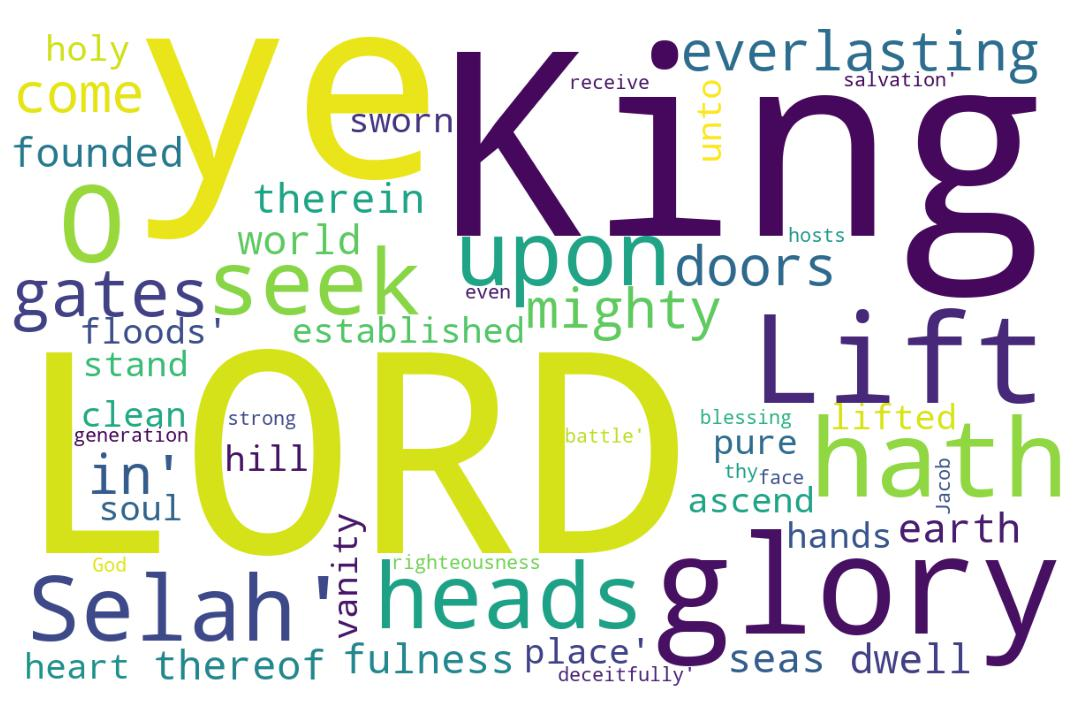
\includegraphics[width=\linewidth]{19OT-Psalms/Psalm24-WordCloud.jpg}
  \caption{Psalm 24 Word Cloud}
  \label{fig:Psalm 24 word Cloud}
\end{figure}


\marginpar{\scriptsize \centering \fcolorbox{bone}{lime}{\textbf{THE COMING KING}}\\ (Psalm 24:1-6) \begin{compactenum}[I.][8]
    \item \textbf{Going} to the King \index[scripture]{Psalms!Psa 024:03}(Psa 24:3)
    \item The \textbf{Godliness} of his Followers \index[scripture]{Psalms!Psa 024:04}(Psa 24:4)
    \item The \textbf{Grace} He Dispenses \index[scripture]{Psalms!Psa 024:05}(Psa 24:5)
    \item The \textbf{Generation} that seeks Him  \index[scripture]{Psalms!Psa 024:06}(Psa 24:6)
    \item A \textbf{Glimpse} of Him \index[scripture]{Psalms!Psa 024:07}\index[scripture]{John!John 18:01}(Psa 24:7, John 18:1)
    \item The \textbf{Gates} of New Jerusalem \index[scripture]{Psalms!Psa 024:07}\index[scripture]{Psalms!Psa 024:09}(Psa 24:7,9), pictured in \index[scripture]{Nehemiah!Neh 02}\index[scripture]{Nehemiah!Neh 003} (Neh 2-3)
    \item His \textbf{Glory} \index[scripture]{Psalms!Psa 024:07}\index[scripture]{Psalms!Psa 024:10}(Psa 24:7,10)
\end{compactenum}}

\marginpar{\scriptsize \centering \fcolorbox{bone}{yellow}{\textbf{REIGNING}}\\ (Psalm 24:1-6) \begin{compactenum}[I.][8]
    \item The \textbf{Hill} \index[scripture]{Psalms!Psa 024:03}(Psa 24:3)
    \item The \textbf{Holy Place} \index[scripture]{Psalms!Psa 024:03}(Psa 24:3)
    \item The \textbf{Heart} \index[scripture]{Psalms!Psa 024:04}(Psa 24:4)
    \item The \textbf{Hands} \index[scripture]{Psalms!Psa 024:04}(Psa 24:4)
    \item The \textbf{Heads} \index[scripture]{Psalms!Psa 024:07}\index[scripture]{Psalms!Psa 024:09}(Psa 24:7 9)
    \item The \textbf{Hosts} \index[scripture]{Psalms!Psa 024:10}(Psa 24:10)
\end{compactenum}}

\marginpar{\scriptsize \centering \fcolorbox{bone}{black}{\textbf{\textcolor[cmyk]{0,0,0,0}{PSALM 24}}}\\ (Psalm 24:1-6) \begin{compactenum}[I.][8]
    \item  \textbf{Existence} of the King \index[scripture]{Psalms!Psa 024:01-02}(Psa 24:1-2)
    \item  \textbf{Elligibility} for the Kingdom \index[scripture]{Psalms!Psa 024:05-06}(Psa 24:5-6)
    \item  \textbf{Entrance} of the King \index[scripture]{Psalms!Psa 024:07-09}(Psa 24:7-9)
    \item  \textbf{Excellence} of the King \index[scripture]{Psalms!Psa 024:10}(Psa 24:10)
\end{compactenum}}

\footnote{\textcolor[cmyk]{0.99998,1,0,0}{\hyperlink{TOC}{Return to end of Table of Contents.}}}\footnote{\href{https://www.audioverse.org/english/audiobibles/books/ENGKJV/O/Ps/1}{\textcolor[cmyk]{0.99998,1,0,0}{Psalms Audio}}}\textcolor[cmyk]{0.99998,1,0,0}{A Psalm of David.}\\
\\
\textcolor[cmyk]{0.99998,1,0,0}{The earth \emph{is} the LORD'S, and the fulness thereof; the world, and they that dwell therein.}\footnote{\textbf{1 Corinthians 10:26, 28} - For the earth is the Lord’s, and the fulness thereof. [28] But if any man say unto you, This is offered in sacrifice unto idols, eat not for his sake that shewed it, and for conscience sake: for the earth is the Lord’s, and the fulness thereof:}\footnote{\textbf{2 Corinthians 4:4} - In whom the god of this world hath blinded the minds of them which believe not, lest the light of the glorious gospel of Christ, who is the image of God, should shine unto them.}
[2] \textcolor[cmyk]{0.99998,1,0,0}{For he hath founded it upon the seas, and established it upon the floods.}
[3] \textcolor[cmyk]{0.99998,1,0,0}{Who shall \fcolorbox{bone}{lime}{ascend} into the hill of the LORD? or who shall stand in his holy place?}\footnote{\textbf{Psalm 2:6} - Yet have I set my king upon my holy hill of Zion.}\footnote{\textbf{Psalm 15:1-5} - LORD, who shall abide in thy tabernacle? who shall dwell in thy holy hill? [2] He that walketh uprightly, and worketh righteousness, and speaketh the truth in his heart. [3] He that backbiteth not with his tongue, nor doeth evil to his neighbour, nor taketh up a reproach against his neighbour. [4] In whose eyes a vile person is contemned; but he honoureth them that fear the LORD. He that sweareth to his own hurt, and changeth not. [5] He that putteth not out his money to usury, nor taketh reward against the innocent. He that doeth these things shall never be moved.}
[4] \textcolor[cmyk]{0.99998,1,0,0}{He that hath \fcolorbox{bone}{lime}{clean hands}, and a \fcolorbox{bone}{lime}{pure heart}; who hath \fcolorbox{bone}{lime}{not lifted up his soul} unto vanity, nor \fcolorbox{bone}{lime}{sworn deceitfully}.}
[5] \textcolor[cmyk]{0.99998,1,0,0}{He shall receive the \fcolorbox{bone}{lime}{blessing} from the LORD, and \fcolorbox{bone}{MYGOLD}{righteousness} from the God of his salvation.}
[6] \textcolor[cmyk]{0.99998,1,0,0}{This \emph{is} the generation of them that \fcolorbox{bone}{lime}{seek} him, that \fcolorbox{bone}{lime}{seek} thy face, O Jacob. Selah.}
[7] \textcolor[cmyk]{0.99998,1,0,0}{\fcolorbox{bone}{lime}{Lift up} your heads, O ye gates; and be ye lift up, ye everlasting \fcolorbox{bone}{lime}{doors}; and the King of \fcolorbox{bone}{lime}{glory} shall come in.}
[8] \textcolor[cmyk]{0.99998,1,0,0}{Who \emph{is} this King of \fcolorbox{bone}{lime}{glory}? The LORD strong and mighty, the LORD mighty in battle.}
[9] \textcolor[cmyk]{0.99998,1,0,0}{Lift up your heads, O ye gates; even lift \emph{them} up, ye everlasting \fcolorbox{bone}{lime}{doors}; and the King of glory shall come in.}
[10] \textcolor[cmyk]{0.99998,1,0,0}{Who is this King of \fcolorbox{bone}{lime}{glory}? The LORD of hosts, he \emph{is} the King of \fcolorbox{bone}{lime}{glory}. Selah.}
\section{Psalm 24 Comments}

\subsection{Numeric Nuggets}
\textbf{4:} The phrase ``king of glory'' is used 4 times (in verses 7, 8, 9, and 10).\\
\\
\textbf{5:} The phrase ``King of glory'' is found 5 times. With 5 being the number of death, this hints at a substitutionary death. All five instances occur after the first of two uses of ``Selah.''\\
\\
\textbf{13:} Verses 1, 5, and 10 have 13 unique words. The 13-letter word ``righteousness'' is used in the chapter.


\subsection{Psalm 24:1}
Verse 1 is a point of theological departure, if one addresses the question, Is the earth the lord's and the fulness thereof?  Obviously, now, if the answer is no, or if it actually was, the Lord would be a spectacularly ineffective ruler in righteousness. The earth is the Lord's, but it is temporarily being ruled by someone else. This is to change.


\subsection{Psalm 24:8-10}

So, who exactly is the ``King of Glory"? Verse 10 answers the question -- the LORD of hosts.  But, for further enlightenment, scripture provides more answers to the ``who is'' question:
\begin{compactenum}
	\item Exodus 15:11 -- Tells us that the ``who is'' is glorious in holiness, fearful in praises, doing wonders,
	\item 1 Samuel 22:4 -- Tells us that the ``who is'' worthy to be praised.
	\item Isaiah 63:1 -- Tells us that the ``who is''  is this that cometh from Edom, with dyed garments from Bozrah? this that is glorious in his apparel, travelling in the greatness of his strength? I that speak in righteousness, mighty to save.
	\item 2 Corinthians 4:4 -- Tells us that the ``who is'' is the image of God, should shine unto them.
	\item Colossians 1:18-20 -- Tells us that the ``who is'' s the beginning, the firstborn from the dead; that in all things he might have the preeminence. [19] For it pleased the Father that in him should all fulness dwell; [20] And, having made peace through the blood of his cross, by him to reconcile all things unto himself; by him, I say, whether they be things in earth, or things in heaven.
	\item Colossians 3:4 -- Tells us that the ``who is'' is our life.
	\item 1 Timothy 6:15 -- Tells us that the ``who is'' is the blessed and only Potentate, the King of kings, and Lord of lords; 16 Who only hath immortality, dwelling in the light which no man can approach unto; whom no man hath seen, nor can see: to whom be honour and power everlasting. Amen. 
	\item Hebrews 7:16 --Tells us that the ``who is'' is made, not after the law of a carnal commandment, but after the power of an endless life.
	\item Hebrews 7:26 -- Tells us that the ``who is'' is holy, harmless, undefiled, separate from sinners, and made higher than the heavens;
	\item Hebrews 7:28 -- Tells us that the ``who is''  is is consecrated for evermore.
	\item Hebrews 8:1 -- Tells us that the ``who is''  is set on the right hand of the throne of the Majesty in the heavens;
	\item Hebrews 11:27 -- Tells us that the ``who is'' is the invisible but omnipotent God.
	\item 1 Peter 3:22 -- Tells us that the ``who is'' is on the right hand of God; angels and authorities and powers being made subject unto him..
	\item Revelation 5:2 -- Tells us that the ``who is'' is the only one worthy to open the book
\end{compactenum}

Consider the popular song, The Little Boy from the Carpenter Shop:

\begin{verbatim}
He was born in a stable, His [Am]mother a virgin; 
raised in a carpenter shop.
His people were slaves, His parents were poor; 
His friends were a lowly lot.
His chances in life, seemed so slim; why, 
He's expected to be a slave.
But the people in darkness saw light in Him; 
as hope for freedom He gave.

[C]All of the power of [Am]heaven and earth;[F] 
God has invested in[C]Him.
[C]He's to die on the cross, [Am]descend into hell; 
meet the [F]devil, take the keys from [G7]him.
He [F]yielded His life to the [G7]death on the cross; 
cried it's [F]finished and then He [G7]died.
In the [C]regions of hell, the [F]devil celebrated; 
we've [C]destroyed the [G7]King, he [C]cried.

In the [C]midst of the celebration, [Am]footsteps were heard; 
walk-[F]ing the corridors of [C]hell.
Then the [C]shouting stopped, as a [Am]voice rang out; 
a [F]voice as clear as a [G7]bell.
[F]Satan then trembled as he [G7]recognized Him; 
who [F]came to deliver His [G7]own.

Oh, [C]shut and lock the [F]gates he cried; 
don't [C]let Him [G7]ascend to His [C]Throne.
Then the [C]gates swung shut in the [Am]face of our LORD; 
to [F]prove salvation [C]untrue.
But, He [C]shook hell's gates, cried [Am]lift up your heads; 
the [F]King is coming [G7]through.

Then out of the devil's prison house 
came a procession led by our King.
Crying out oh grave, where [F]is thy victory; 
and death where is thy [C]sting?
Who is the [F]King of Glory? 
The LORD GOD ALMIGHTY; that is He.
Who is the King of Glory? 
He's the master of the host of heaven supreme.

[C]Who is the [F]King of Glory? 
He's the one that not even death could [C]stop!
[C]Who [G7]is the King of Glory? 
The Little Boy from the Carpenter [C]Shop[~F~C]
[C]The Little [G7]Boy from the Carpenter [F]Shop![~~C]
\end{verbatim}
%\input{19OT-Psalms/Psalm24WordIndex}
\section{Psalm 24 Outlines}

\subsection{My Outlines}

\subsubsection{The Coming King}

\index[speaker]{Keith Anthony!Psalm 024 (The Coming King)}
\index[series]{Psalms (Keith Anthony)!Psalm 024 (The Coming King)}
\index[date]{2016/06/30!Psalm 024 (The Coming King) (Keith Anthony)}
\index[EVENTS]{Xenia Rest Home!Psalm 24 - The Coming King!2019 May 19}

\begin{compactenum}[I.]
    \item \textbf{Going} to the King \index[scripture]{Psalms!Psa 024:03}(Psa 24:3)
    \item The \textbf{Godliness} of his Followers \index[scripture]{Psalms!Psa 024:04}(Psa 24:4)
    \item The \textbf{Grace} He Dispenses \index[scripture]{Psalms!Psa 024:05}(Psa 24:5)
    \item The \textbf{Generation} that sees Him take the Throne \index[scripture]{Psalms!Psa 024:06}(Psa 24:6)
    \item A \textbf{Glimpse} of Him \index[scripture]{Psalms!Psa 024:07}\index[scripture]{John!John 18:01}(Psa 24:7, John 18:1)
    \item The \textbf{Gates} of New Jerusalem \index[scripture]{Psalms!Psa 024:07}\index[scripture]{Psalms!Psa 024:09}(Psalm 24:7,9), pictured in \index[scripture]{Nehemiah!Neh 02}\index[scripture]{Nehemiah!Neh 003}Neh 2-3
    \item His \textbf{Glory} \index[scripture]{Psalms!Psa 024:07}\index[scripture]{Psalms!Psa 024:10}(Psa 24:7,10)
\end{compactenum}

\subsubsection{Reigning}
\index[speaker]{Keith Anthony!Psalm 024 (Reigning)}
\index[series]{Psalms (Keith Anthony)!Psalm 024 (Reigning)}
\index[date]{2019/01/24!Psalm 024 (Reigning) (Keith Anthony)}
\begin{compactenum}[I.]
    \item The \textbf{Hill} \index[scripture]{Psalms!Psa 024:03}(Psalm 24:3)
    \item The \textbf{Holy Place} \index[scripture]{Psalms!Psa 024:03}(Psa 24:3)
    \item The \textbf{Heart} \index[scripture]{Psalms!Psa 024:04}(Psa 24:4)
    \item The \textbf{Hands} \index[scripture]{Psalms!Psa 024:04}(Psa 24:4)
    \item The \textbf{Heads} \index[scripture]{Psalms!Psa 024:07}\index[scripture]{Psalms!Psa 024:09}(Psa 24:7, 9)
    \item The \textbf{Hosts} \index[scripture]{Psalms!Psa 024:10}(Psa 24:10)
\end{compactenum}

\subsubsection{Psalm 24}
\index[speaker]{Keith Anthony!Psalm 024 (Psalm 24)}
\index[series]{Psalms (Keith Anthony)!Psalm 024 (Psalm 24)}
\index[date]{2019/01/24!Psalm 024 (Psalm 24) (Keith Anthony)} \begin{compactenum}[I.][8]
    \item  \textbf{Existence} of the King \index[scripture]{Psalms!Psa 024:01-02}(Psa 24:1-2)
    \item  \textbf{Elligibility} for the Kingdom \index[scripture]{Psalms!Psa 024:05-06}(Psa 24:5-6)
    \item  \textbf{Entrance} of the King \index[scripture]{Psalms!Psa 024:07-09}(Psa 24:7-9)
    \item  \textbf{Excellence} of the King \index[scripture]{Psalms!Psa 024:10}(Psa 24:10)
\end{compactenum}

\subsection{Outlines from Others}




%\section{Psalm 24 Statistics}

%%%%%%%%%%%%%%%%%%%%%%%%%%%
%%%%% Word Statistics
%%%%%%%%%%%%%%%%%%%%%%%%%%


\normalsize



\subsection{Chapter Word Statistics}


%%%%%%%%%%
%%%%%%%%%%
 
\begin{center}
\begin{longtable}{l|c|c|c|c}
\caption[Stats for Psalm 24]{Stats for Psalm 24} \label{table:Stats for Psalm 24} \\ 
\hline \multicolumn{1}{|c|}{\textbf{Verse(s)}} & \multicolumn{1}{|c|}{\textbf{Count}} & \multicolumn{1}{|c|}{\textbf{Unique}} & \multicolumn{1}{|c|}{\textbf{Italics}} & \multicolumn{1}{|c|}{\textbf{Uniq Italic}}  \\ \hline 
\endfirsthead
 
\multicolumn{5}{c}
{{\bfseries \tablename\ \thetable{} -- continued from previous page}} \\  
\hline \multicolumn{1}{|c|}{\textbf{Verse(s)}} & \multicolumn{1}{|c|}{\textbf{Count}} & \multicolumn{1}{|c|}{\textbf{Unique}} & \multicolumn{1}{|c|}{\textbf{Italics}} & \multicolumn{1}{|c|}{\textbf{Uniq Italic}}  \\ \hline 
\endhead
 
\hline \multicolumn{5}{|r|}{{Continued if needed}} \\ \hline
\endfoot 
1 & 16 & 13 & 1 & 1\\ \hline
2 & 14 & 11 & 0 & 0\\ \hline
3 & 17 & 15 & 0 & 0\\ \hline
4 & 21 & 20 & 0 & 0\\ \hline
5 & 16 & 13 & 0 & 0\\ \hline
6 & 16 & 14 & 1 & 1\\ \hline
7 & 23 & 19 & 0 & 0\\ \hline
8 & 16 & 14 & 1 & 1\\ \hline
9 & 22 & 20 & 1 & 1\\ \hline
10 & 17 & 13 & 1 & 1\\ \hline
\hline \hline
Total & 178 & 87 & 5 & 2



\end{longtable}
\end{center}

%%%%%%%%%%
%%%%%%%%%%
 
\subsection{Words by Frequency}


\begin{center}
\begin{longtable}{l|r}
\caption[Word Frequencies in Psalm 24]{Word Frequencies in Psalm 24} \label{table:WordsIn-Psalm-24} \\ 
\hline \multicolumn{1}{|c|}{\textbf{Word}} & \multicolumn{1}{c|}{\textbf{Frequency}} \\ \hline 
\endfirsthead
 
\multicolumn{2}{c}
{{\bfseries \tablename\ \thetable{} -- continued from previous page}} \\ 
\hline \multicolumn{1}{|c|}{\textbf{Word}} & \multicolumn{1}{c|}{\textbf{Frequency}} \\ \hline 
\endhead
 
\hline \multicolumn{2}{|r|}{{Continued if needed}} \\ \hline
\endfoot
 
\hline \hline
\endlastfoot
the & 15 \\ \hline
and & 9 \\ \hline
of & 9 \\ \hline
shall & 5 \\ \hline
LORD & 5 \\ \hline
up & 5 \\ \hline
ye & 5 \\ \hline
King & 5 \\ \hline
glory & 5 \\ \hline
\emph{is} & 4 \\ \hline
that & 4 \\ \hline
in & 4 \\ \hline
The & 3 \\ \hline
hath & 3 \\ \hline
Who & 3 \\ \hline
his & 3 \\ \hline
O & 3 \\ \hline
he & 2 \\ \hline
it & 2 \\ \hline
upon & 2 \\ \hline
who & 2 \\ \hline
He & 2 \\ \hline
from & 2 \\ \hline
seek & 2 \\ \hline
Selah & 2 \\ \hline
Lift & 2 \\ \hline
your & 2 \\ \hline
heads & 2 \\ \hline
gates & 2 \\ \hline
lift & 2 \\ \hline
everlasting & 2 \\ \hline
doors & 2 \\ \hline
come & 2 \\ \hline
this & 2 \\ \hline
mighty & 2 \\ \hline
earth & 1 \\ \hline
LORD'S & 1 \\ \hline
fulness & 1 \\ \hline
thereof & 1 \\ \hline
world & 1 \\ \hline
they & 1 \\ \hline
dwell & 1 \\ \hline
therein & 1 \\ \hline
For & 1 \\ \hline
founded & 1 \\ \hline
seas & 1 \\ \hline
established & 1 \\ \hline
floods & 1 \\ \hline
ascend & 1 \\ \hline
into & 1 \\ \hline
hill & 1 \\ \hline
or & 1 \\ \hline
stand & 1 \\ \hline
holy & 1 \\ \hline
place & 1 \\ \hline
clean & 1 \\ \hline
hands & 1 \\ \hline
a & 1 \\ \hline
pure & 1 \\ \hline
heart & 1 \\ \hline
not & 1 \\ \hline
lifted & 1 \\ \hline
soul & 1 \\ \hline
unto & 1 \\ \hline
vanity & 1 \\ \hline
nor & 1 \\ \hline
sworn & 1 \\ \hline
deceitfully & 1 \\ \hline
receive & 1 \\ \hline
blessing & 1 \\ \hline
righteousness & 1 \\ \hline
God & 1 \\ \hline
salvation & 1 \\ \hline
This & 1 \\ \hline
generation & 1 \\ \hline
them & 1 \\ \hline
him & 1 \\ \hline
thy & 1 \\ \hline
face & 1 \\ \hline
Jacob & 1 \\ \hline
be & 1 \\ \hline
strong & 1 \\ \hline
battle & 1 \\ \hline
even & 1 \\ \hline
\emph{them} & 1 \\ \hline
is & 1 \\ \hline
hosts & 1 \\ \hline
\end{longtable}
\end{center}



\normalsize



\subsection{Words Alphabetically}


\begin{center}
\begin{longtable}{l|r}
\caption[Word Alphabetically in Psalm 24]{Word Alphabetically in Psalm 24} \label{table:WordsIn-Psalm-24} \\ 
\hline \multicolumn{1}{|c|}{\textbf{Word}} & \multicolumn{1}{c|}{\textbf{Frequency}} \\ \hline 
\endfirsthead
 
\multicolumn{2}{c}
{{\bfseries \tablename\ \thetable{} -- continued from previous page}} \\ 
\hline \multicolumn{1}{|c|}{\textbf{Word}} & \multicolumn{1}{c|}{\textbf{Frequency}} \\ \hline 
\endhead
 
\hline \multicolumn{2}{|r|}{{Continued if needed}} \\ \hline
\endfoot
 
\hline \hline
\endlastfoot
For & 1 \\ \hline
God & 1 \\ \hline
He & 2 \\ \hline
Jacob & 1 \\ \hline
King & 5 \\ \hline
LORD & 5 \\ \hline
LORD'S & 1 \\ \hline
Lift & 2 \\ \hline
O & 3 \\ \hline
Selah & 2 \\ \hline
The & 3 \\ \hline
This & 1 \\ \hline
Who & 3 \\ \hline
\emph{is} & 4 \\ \hline
\emph{them} & 1 \\ \hline
a & 1 \\ \hline
and & 9 \\ \hline
ascend & 1 \\ \hline
battle & 1 \\ \hline
be & 1 \\ \hline
blessing & 1 \\ \hline
clean & 1 \\ \hline
come & 2 \\ \hline
deceitfully & 1 \\ \hline
doors & 2 \\ \hline
dwell & 1 \\ \hline
earth & 1 \\ \hline
established & 1 \\ \hline
even & 1 \\ \hline
everlasting & 2 \\ \hline
face & 1 \\ \hline
floods & 1 \\ \hline
founded & 1 \\ \hline
from & 2 \\ \hline
fulness & 1 \\ \hline
gates & 2 \\ \hline
generation & 1 \\ \hline
glory & 5 \\ \hline
hands & 1 \\ \hline
hath & 3 \\ \hline
he & 2 \\ \hline
heads & 2 \\ \hline
heart & 1 \\ \hline
hill & 1 \\ \hline
him & 1 \\ \hline
his & 3 \\ \hline
holy & 1 \\ \hline
hosts & 1 \\ \hline
in & 4 \\ \hline
into & 1 \\ \hline
is & 1 \\ \hline
it & 2 \\ \hline
lift & 2 \\ \hline
lifted & 1 \\ \hline
mighty & 2 \\ \hline
nor & 1 \\ \hline
not & 1 \\ \hline
of & 9 \\ \hline
or & 1 \\ \hline
place & 1 \\ \hline
pure & 1 \\ \hline
receive & 1 \\ \hline
righteousness & 1 \\ \hline
salvation & 1 \\ \hline
seas & 1 \\ \hline
seek & 2 \\ \hline
shall & 5 \\ \hline
soul & 1 \\ \hline
stand & 1 \\ \hline
strong & 1 \\ \hline
sworn & 1 \\ \hline
that & 4 \\ \hline
the & 15 \\ \hline
them & 1 \\ \hline
therein & 1 \\ \hline
thereof & 1 \\ \hline
they & 1 \\ \hline
this & 2 \\ \hline
thy & 1 \\ \hline
unto & 1 \\ \hline
up & 5 \\ \hline
upon & 2 \\ \hline
vanity & 1 \\ \hline
who & 2 \\ \hline
world & 1 \\ \hline
ye & 5 \\ \hline
your & 2 \\ \hline
\end{longtable}
\end{center}



\normalsize



\subsection{Word Lengths in Chapter}
\normalsize
\begin{longtable}{l|p{3.75in}}
\caption[Words by Length in Psalm 24]{Words by Length in Psalm 24} \label{table:WordsIn-Psalm-24} \\ 
\hline \multicolumn{1}{|c|}{\textbf{Length}} & \multicolumn{1}{c|}{\textbf{Words}} \\ \hline 
\endfirsthead
 
\multicolumn{2}{c}
{{\bfseries \tablename\ \thetable{} -- continued from previous page}} \\ 
\hline \multicolumn{1}{|c|}{\textbf{Length}} & \multicolumn{1}{c|}{\textbf{Words}} \\ \hline 
\endhead
 
\hline \multicolumn{2}{|r|}{{Continued if needed}} \\ \hline
\endfoot
 
\hline \hline
\endlastfoot
1 & a, O \\ \hline
2 & \emph{is}, he, it, of, or, in, He, up, ye, be, is \\ \hline
3 & The, the, and, For, Who, who, his, not, nor, God, him, thy \\ \hline
4 & they, that, hath, upon, seas, into, hill, LORD, holy, pure, soul, unto, from, This, them, seek, face, Lift, your, lift, King, come, this, even, \emph{them} \\ \hline
5 & earth, world, dwell, shall, stand, place, clean, hands, heart, sworn, Jacob, Selah, heads, gates, doors, glory, hosts \\ \hline
6 & LORD'S, floods, ascend, lifted, vanity, strong, mighty, battle \\ \hline
7 & fulness, thereof, therein, founded, receive \\ \hline
8 & blessing \\ \hline
9 & salvation \\ \hline
10 & generation \\ \hline
11 & established, deceitfully, everlasting \\ \hline
13 & righteousness \\ \hline
\end{longtable}






%%%%%%%%%%
%%%%%%%%%%
\subsection{Psalm 24 Repeated Phrases}


%%%%%%%%%%
%%%%%%%%%%
\normalsize
 
\begin{center}
\begin{longtable}{|p{3.0in}|p{0.5in}|}
\caption[Psalm 24 Repeated Phrases]{Psalm 24 Repeated Phrases}\label{table:Repeated Phrases Psalm 24} \\
\hline \multicolumn{1}{|c|}{\textbf{Phrase}} & \multicolumn{1}{c|}{\textbf{Frequency}} \\ \hline 
\endfirsthead
 
\multicolumn{2}{c}
{{\bfseries \tablename\ \thetable{} -- continued from previous page}} \\  
\hline \multicolumn{1}{|c|}{\textbf{Phrase}} & \multicolumn{1}{c|}{\textbf{Frequency}} \\ \hline 
\endhead
 
\hline \multicolumn{2}{c}{{ }} \\ \hline
\endfoot 
King of & 5\\ \hline 
King of glory & 5\\ \hline 
of glory & 5\\ \hline 
\emph{is} the & 3\\ \hline 
and the & 3\\ \hline 
the LORD & 3\\ \hline 
the King & 3\\ \hline 
the King of & 3\\ \hline 
the King of glory & 3\\ \hline 
\end{longtable}
\end{center}



%%%%%%%%%%
%%%%%%%%%%




\chapter{Psalm 25}

\begin{figure}
  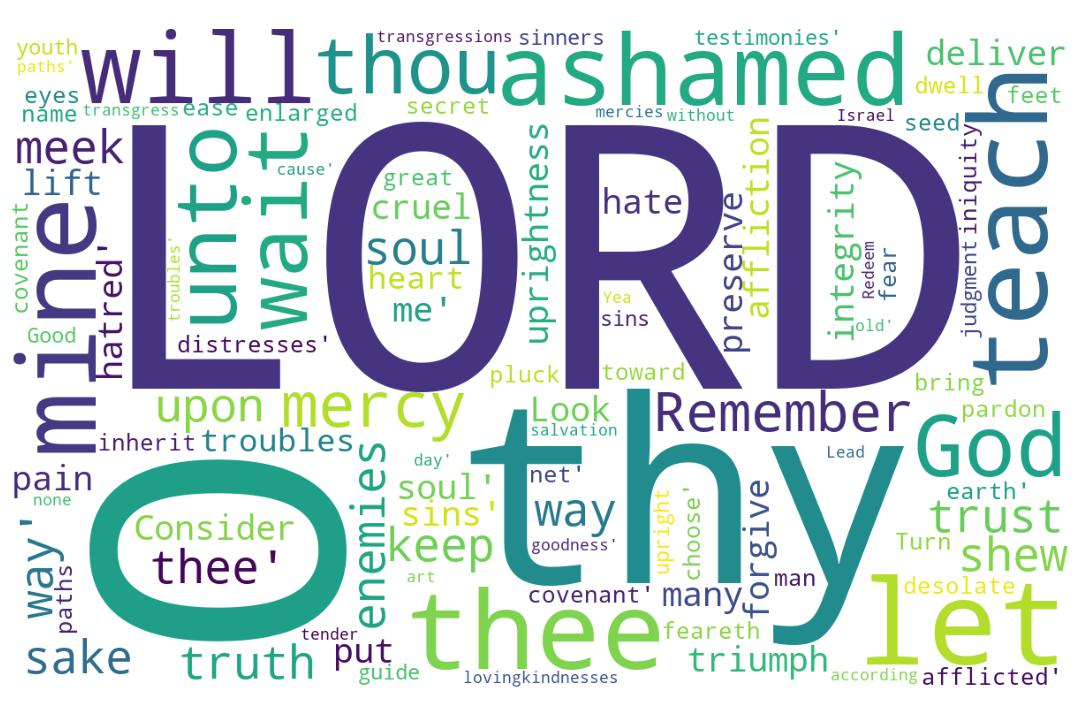
\includegraphics[width=\linewidth]{19OT-Psalms/Psalm25-WordCloud.jpg}
  \caption{Psalm 25 Word Cloud}
  \label{fig:Psalm 25 word Cloud}
\end{figure}

\marginpar{\scriptsize \centering \fcolorbox{bone}{lime}{\textbf{DAVID'S PRAYER}}\\ (Psalm 25:16--22) \begin{compactenum}[I.][8]
     \item \textbf{Turn unto Me}  \index[scripture]{Psalms!Psa 025:16}(Psa 25:16)
    \item \textbf{Bring Me out of Distress} \index[scripture]{Psalms!Psa 025:17}(Psa 25:17)
    \item \textbf{Attend to My Affliction}  \index[scripture]{Psalms!Psa 025:18}(Psa 25:18)
    \item \textbf{Take Care of My Enemies}  \index[scripture]{Psalms!Psa 025:19}(Psa 25:19)
    \item \textbf{Deliver Me}
    \item \textbf{Preserve Me} \index[scripture]{Psalms!Psa 025:21}(Psa 25:21)
    \item \textbf{Redeem Me} \index[scripture]{Psalms!Psa 025:22}(Psa 25:22)
\end{compactenum}}

\footnote{\textcolor[cmyk]{0.99998,1,0,0}{\hyperlink{TOC}{Return to end of Table of Contents.}}}\footnote{\href{https://www.audioverse.org/english/audiobibles/books/ENGKJV/O/Ps/1}{\textcolor[cmyk]{0.99998,1,0,0}{Psalms Audio}}}\textcolor[cmyk]{0.99998,1,0,0}{\emph{A Psalm} of David.}\\
\\
\textcolor[cmyk]{0.99998,1,0,0}{Unto thee, O LORD, do I lift up my soul.}
[2] \textcolor[cmyk]{0.99998,1,0,0}{O my God, I trust in thee: let me not be ashamed, let not mine enemies triumph over me.}
[3] \textcolor[cmyk]{0.99998,1,0,0}{Yea, let none that wait on thee be ashamed: let them be ashamed which transgress without cause.}
[4] \textcolor[cmyk]{0.99998,1,0,0}{Shew me thy ways, O LORD; teach me thy paths.}
[5] \textcolor[cmyk]{0.99998,1,0,0}{Lead me in thy truth, and teach me: for thou \emph{art} the God of my salvation; on thee do I wait all the day.}
[6] \textcolor[cmyk]{0.99998,1,0,0}{Remember, O LORD, thy tender mercies and thy lovingkindnesses; for they \emph{have} \emph{been} ever of old.}
[7] \textcolor[cmyk]{0.99998,1,0,0}{Remember not the sins of my youth, nor my transgressions: according to thy mercy remember thou me for thy goodness' sake, O LORD.}
[8] \textcolor[cmyk]{0.99998,1,0,0}{Good and upright \emph{is} the LORD: therefore will he teach sinners in the way.}
[9] \textcolor[cmyk]{0.99998,1,0,0}{The meek will he guide in judgment: and the meek will he teach his way.}
[10] \textcolor[cmyk]{0.99998,1,0,0}{All the paths of the LORD \emph{are} mercy and truth unto such as keep his covenant and his testimonies.}
[11] \textcolor[cmyk]{0.99998,1,0,0}{For thy name's sake, O LORD, pardon mine iniquity; for it \emph{is} great.}
[12] \textcolor[cmyk]{0.99998,1,0,0}{What man \emph{is} he that feareth the LORD? him shall he teach in the way \emph{that} he shall choose.}
[13] \textcolor[cmyk]{0.99998,1,0,0}{His soul shall dwell at ease; and his seed shall inherit the earth.}
[14] \textcolor[cmyk]{0.99998,1,0,0}{The secret of the LORD \emph{is} with them that fear him; and he will shew them his covenant.}
[15] \textcolor[cmyk]{0.99998,1,0,0}{Mine eyes \emph{are} ever toward the LORD; for he shall pluck my feet out of the net.}
[16] \textcolor[cmyk]{0.99998,1,0,0}{\fcolorbox{bone}{lime}{Turn thee} unto me, and have mercy upon me; for I \emph{am} desolate and afflicted.}
[17] \textcolor[cmyk]{0.99998,1,0,0}{The troubles of my heart are enlarged: \emph{O} bring thou me out of \fcolorbox{bone}{lime}{my distresses}.}\footnote{\textbf{Isaiah 6:10} -- Make the heart of this people fat, and make their ears heavy, and shut their eyes; lest they see with their eyes, and hear with their ears, and understand with their heart, and convert, and be healed.}
[18] \textcolor[cmyk]{0.99998,1,0,0}{Look \fcolorbox{bone}{lime}{upon mine affliction} and my pain; and forgive all my sins.}
[19] \textcolor[cmyk]{0.99998,1,0,0}{Consider \fcolorbox{bone}{lime}{mine enemies}; for they are many; and they hate me with cruel hatred.}
[20] \textcolor[cmyk]{0.99998,1,0,0}{O keep my soul, and deliver me: let me not be ashamed; for I put my trust in thee.}
[21] \textcolor[cmyk]{0.99998,1,0,0}{Let integrity and uprightness \fcolorbox{bone}{lime}{preserve me}; for I wait on thee.}
[22] \textcolor[cmyk]{0.99998,1,0,0}{\fcolorbox{bone}{lime}{Redeem Israel}, O God, out of all his troubles.}

\section{Psalm 25 Comments}

\subsection{Numeric Nuggets}
Verses Psalm 24:11 and 24:13 have 13 words.

%%% Ruckman notes
%%  This is by far the simplest Psalm we have had to deal with yet. It contains more purely devotional material than any one of the preceding twenty-four. Yet even in this one, we find an ending inserted that says “Redeem Israel, O God, out of all his troubles,” which lands us right back into Daniel’s Seventieth Week again. But there are twentyone verses that any saint in any dispensation could profitably apply to his own condition and circumstances. Any saint’s soul should “wait” on God (vs. 3), trust in God (vs. 2), and look up to God (vs. 1). If the Lord shows you His “ways” and teaches you His “paths” (vs. 4), then you will rightly divide the word of truth (2 Tim. 2:15) and not be “ashamed” (vs. 3). No one can find 2 Timothy 2:15 in any English Bible any more unless he goes by the “King James Only,” to cite the Alexandrian Cult’s terminology, for God’s preservation of this unique truth is not found in the ASV, NASV, NIV, RSV, NRSV, RV, or NKJV. “Let not mine enemies triumph over me” is a legitimate prayer for any saint endangered by enemies, although the “grounds” for getting this prayer answered differ as much as David’s case differs from Paul’s. “Them...which transgress without cause” is very interesting for it shows that some folks have a CAUSE or REASON for transgressing even if God doesn’t accept it. Whosoever is angry with his brother “without a cause” (Matt. 5:22) is in danger, but Paul says that if there is a CAUSE, “Be ye angry” (Eph. 4:26). The transgression here means a trespass against the speaker, when the speaker (David) has done nothing to warrant the trespass. An exact case is Saul when he hunts him down to kill him. There are four requests in the prayer: 1. SHEW ME (vs. 4). 2. TEACH ME (vs. 4). 3. LEAD ME (vs. 5). 4. REMEMBER ME (vs. 7). In line with the last request, the Lord “remembered Noah” (Gen. 8:1), but not for his drinking. Noah is pictured in Hebrews 11:7 without fault. The Lord “remembered Rachel” (Gen. 30:22), but did not “remember” the “sins of her youth.” He doesn’t mention Rachel stealing her daddy’s “gods” in the New Testament (Matt. 2:18). God’s “tender mercies” and “loving kindnesses” are manifest throughout the Scriptures and then are manifest in the lives of New Testament Christians for centuries. It is true that many of the saints taste the hellish circumstances of Hebrews 11:36–37, but these are the chosen “elect” for the martyr’s crown. Millions of Christians have come and gone off the face of this earth with no moresorrow and pain than that experienced by all of their unsaved neighbors around them, and these saints had the benefits of eternal security, the presence of Christ, the comfort of the Holy Spirit, and “handfuls of purpose” (Ruth 2:16) dumped out to them while they were going through the trials. 

%% There is nothing “Messianic” about verses 7 and 11. This is David. He is praying for forgiveness of sin in verse 18. God will teach because He is good (vs. 8), but it must be “in the way” (vs. 8) because He is “the way, the truth, and the life” (John 14:6). This means that “the way” must be “his way” (vs. 9). Notice how Rebekah, a type of the Bride of Christ, has to go “his way” (Gen. 24:61)— Eliezer’s way, who is a type of the Holy Spirit. The instruction is promised to only one kind of a Christian: a meek Christian (vs. 9). This is one of the fruits of the Holy Spirit found in Galatians 5:23; it has to do with the heart attitude of the saint in relation to God— NOT MAN. Observe that the man who was “meek above all the men” upon the earth (Num. 12:3) was a KILLER (Ex. 2:12), who lost his temper on more than one occasion (Ex. 32:19; Num. 20:10–11). You see, these modern, humanistic liberals have been teaching Christians a lie, and they have repeated their little “turn the cheek” bit so often that modern Christians think that a Christian is a milk sop who lies down flat on his face every time a jackass walks into the house, or who kisses and hugs every Biblerejecting, Christ-denying, God-hating hellcat on earth. That is not what the word “meek” means in the book. Observe, in verse 9, that you cannot “guide” a bucking bronco or a stubborn ass anywhere. When a horse got his rear foot caught in the stirrup while trying to scratch himself, his rider said, “Listen bud, they’re ain’t room for two of us up here, and if you’re going to drive, I’m gettin’ off!” “His covenant and his testimonies” land us back on Israel again in the works and faith setup of the Old Testament, but still there is spiritual truth if you want to talk about a Christian “living for the Lord.” All the paths of the Lord are TRUTH even when the path is dark and thorny, or going uphill. None of the Lord’s paths are crooked (see Prov. 2:13, 15, 20). The prayers of David for forgiveness (see vss. 11, 18) are a “no-no” to the Dry Cleaners (Stam, Baker, O’Hair, Bullinger, Ballard, Watkins, Moore, Brock, Sharpe, et al.), for these Antinomians who are wrongly dividing the word of truth assume that you “make the cross of none effect” or become an “enemy of the cross of Christ” if you ask for forgiveness AFTER salvation because Calvary “covers it all.” The dry cleaned “idjits” don’t realize that sin can break your fellowship with the Lord, no matter if ALL of them were paid for eternally. Their thinking is that you can get back into fellowship with the Lord without apologizing for lying to the Holy Spirit (Acts 5:3), grieving the Holy Spirit (Eph. 4:30), and quenching the Holy Spirit (1 Thess. 5:19). The hyper-dispensational “grace position” (Bullinger, Baker, and Stam were all five point TULIP hyper-Calvinists) is that a son can stay in fellowship with a father after tearing the curtains down, cutting up the rug, burning the bed sheets, and dumping ink on the pillow cases, by saying, “Thank you for taking care of this at Calvary.” It doesn’t work that way. Christians who take that “grace” position are WEAK spiritually and SICK physically, and many are DEAD (1 Cor. 11:30). If you want to know why no dry cleaning “Hyper” ever did one really spiritual work for God in a century it is because God will not honor this attitude about sin. He dumps them.


%\input{19OT-Psalms/Psalm25WordIndex}
\section{Psalm 25 Outlines}

\subsection{My Outlines}

\subsubsection{David's Prayer}

\index[speaker]{Keith Anthony!Psalm 025 (David's Prayer)}
\index[series]{Psalms (Keith Anthony)!Psalm 025 (David's Prayer)}
\index[date]{2016/07/01!Psalm 025 (David's Prayer) (Keith Anthony)}

\begin{compactenum}[I.]
     \item \textbf{Turn unto Me}  \index[scripture]{Psalms!Psa 025:16}(Psa 25:16)
    \item \textbf{Bring Me out of Distress} \index[scripture]{Psalms!Psa 025:17}(Psa 25:17)
    \item \textbf{Attend to My Affliction}  \index[scripture]{Psalms!Psa 025:18}(Psa 25:18)
    \item \textbf{Take Care of My Enemies}  \index[scripture]{Psalms!Psa 025:19}(Psa 25:19)
    \item \textbf{Deliver Me}
    \item \textbf{Preserve Me} \index[scripture]{Psalms!Psa 025:21}(Psa 25:21)
    \item \textbf{Redeem Me} \index[scripture]{Psalms!Psa 025:22}(Psa 25:22)
\end{compactenum}



\subsection{Outlines from Others}



%\section{Psalm 25 Statistics}

%%%%%%%%%%%%%%%%%%%%%%%%%%%
%%%%%Word Statistics
%%%%%%%%%%%%%%%%%%%%%%%%%%%


\normalsize



\subsection{Chapter Word Statistics}


%%%%%%%%%%
%%%%%%%%%%
 
\begin{center}
\begin{longtable}{l|c|c|c|c}
\caption[Stats for Psalm 25]{Stats for Psalm 25} \label{table:Stats for Psalm 25} \\ 
\hline \multicolumn{1}{|c|}{\textbf{Verse(s)}} & \multicolumn{1}{|c|}{\textbf{Count}} & \multicolumn{1}{|c|}{\textbf{Unique}} & \multicolumn{1}{|c|}{\textbf{Italics}} & \multicolumn{1}{|c|}{\textbf{Uniq Italic}}  \\ \hline 
\endfirsthead
 
\multicolumn{5}{c}
{{\bfseries \tablename\ \thetable{} -- continued from previous page}} \\  
\hline \multicolumn{1}{|c|}{\textbf{Verse(s)}} & \multicolumn{1}{|c|}{\textbf{Count}} & \multicolumn{1}{|c|}{\textbf{Unique}} & \multicolumn{1}{|c|}{\textbf{Italics}} & \multicolumn{1}{|c|}{\textbf{Uniq Italic}}  \\ \hline 
\endhead
 
\hline \multicolumn{5}{|r|}{{Continued if needed}} \\ \hline
\endfoot 
1 & 10 & 10 & 0 & 0\\ \hline
2 & 19 & 16 & 0 & 0\\ \hline
3 & 17 & 14 & 0 & 0\\ \hline
4 & 10 & 8 & 0 & 0\\ \hline
5 & 24 & 22 & 1 & 1\\ \hline
6 & 16 & 15 & 2 & 2\\ \hline
7 & 23 & 21 & 0 & 0\\ \hline
8 & 14 & 13 & 1 & 1\\ \hline
9 & 15 & 12 & 0 & 0\\ \hline
10 & 19 & 16 & 1 & 1\\ \hline
11 & 13 & 13 & 1 & 1\\ \hline
12 & 19 & 15 & 2 & 2\\ \hline
13 & 13 & 12 & 0 & 0\\ \hline
14 & 18 & 17 & 1 & 1\\ \hline
15 & 17 & 16 & 1 & 1\\ \hline
16 & 15 & 13 & 1 & 1\\ \hline
17 & 15 & 13 & 1 & 1\\ \hline
18 & 12 & 10 & 0 & 0\\ \hline
19 & 14 & 13 & 0 & 0\\ \hline
20 & 19 & 17 & 0 & 0\\ \hline
21 & 11 & 11 & 0 & 0\\ \hline
22 & 9 & 9 & 0 & 0\\ \hline
\hline \hline
Total & 342 & 149 & 12 & 8



\end{longtable}
\end{center}

%%%%%%%%%%
%%%%%%%%%%
 
\subsection{Words by Frequency}

\begin{center}
\begin{longtable}{l|r}
\caption[Word Frequencies in Psalm 25]{Word Frequencies in Psalm 25} \label{table:WordsIn-Psalm-25} \\ 
\hline \multicolumn{1}{|c|}{\textbf{Word}} & \multicolumn{1}{c|}{\textbf{Frequency}} \\ \hline 
\endfirsthead
 
\multicolumn{2}{c}
{{\bfseries \tablename\ \thetable{} -- continued from previous page}} \\ 
\hline \multicolumn{1}{|c|}{\textbf{Word}} & \multicolumn{1}{c|}{\textbf{Frequency}} \\ \hline 
\endhead
 
\hline \multicolumn{2}{|r|}{{Continued if needed}} \\ \hline
\endfoot
 
\hline \hline
\endlastfoot
and & 15 \\ \hline
me & 14 \\ \hline
the & 14 \\ \hline
my & 12 \\ \hline
LORD & 10 \\ \hline
for & 9 \\ \hline
of & 9 \\ \hline
O & 8 \\ \hline
thy & 8 \\ \hline
he & 8 \\ \hline
thee & 7 \\ \hline
I & 6 \\ \hline
in & 6 \\ \hline
his & 6 \\ \hline
let & 5 \\ \hline
teach & 5 \\ \hline
shall & 5 \\ \hline
not & 4 \\ \hline
be & 4 \\ \hline
ashamed & 4 \\ \hline
mine & 4 \\ \hline
\emph{is} & 4 \\ \hline
will & 4 \\ \hline
soul & 3 \\ \hline
God & 3 \\ \hline
that & 3 \\ \hline
wait & 3 \\ \hline
on & 3 \\ \hline
them & 3 \\ \hline
thou & 3 \\ \hline
all & 3 \\ \hline
they & 3 \\ \hline
mercy & 3 \\ \hline
way & 3 \\ \hline
The & 3 \\ \hline
out & 3 \\ \hline
do & 2 \\ \hline
trust & 2 \\ \hline
enemies & 2 \\ \hline
paths & 2 \\ \hline
truth & 2 \\ \hline
Remember & 2 \\ \hline
ever & 2 \\ \hline
sins & 2 \\ \hline
sake & 2 \\ \hline
meek & 2 \\ \hline
\emph{are} & 2 \\ \hline
unto & 2 \\ \hline
keep & 2 \\ \hline
covenant & 2 \\ \hline
him & 2 \\ \hline
with & 2 \\ \hline
upon & 2 \\ \hline
troubles & 2 \\ \hline
are & 2 \\ \hline
Unto & 1 \\ \hline
lift & 1 \\ \hline
up & 1 \\ \hline
triumph & 1 \\ \hline
over & 1 \\ \hline
Yea & 1 \\ \hline
none & 1 \\ \hline
which & 1 \\ \hline
transgress & 1 \\ \hline
without & 1 \\ \hline
cause & 1 \\ \hline
Shew & 1 \\ \hline
ways & 1 \\ \hline
Lead & 1 \\ \hline
\emph{art} & 1 \\ \hline
salvation & 1 \\ \hline
day & 1 \\ \hline
tender & 1 \\ \hline
mercies & 1 \\ \hline
lovingkindnesses & 1 \\ \hline
\emph{have} & 1 \\ \hline
\emph{been} & 1 \\ \hline
old & 1 \\ \hline
youth & 1 \\ \hline
nor & 1 \\ \hline
transgressions & 1 \\ \hline
according & 1 \\ \hline
to & 1 \\ \hline
remember & 1 \\ \hline
goodness' & 1 \\ \hline
Good & 1 \\ \hline
upright & 1 \\ \hline
therefore & 1 \\ \hline
sinners & 1 \\ \hline
guide & 1 \\ \hline
judgment & 1 \\ \hline
All & 1 \\ \hline
such & 1 \\ \hline
as & 1 \\ \hline
testimonies & 1 \\ \hline
For & 1 \\ \hline
name's & 1 \\ \hline
pardon & 1 \\ \hline
iniquity & 1 \\ \hline
it & 1 \\ \hline
great & 1 \\ \hline
What & 1 \\ \hline
man & 1 \\ \hline
feareth & 1 \\ \hline
\emph{that} & 1 \\ \hline
choose & 1 \\ \hline
His & 1 \\ \hline
dwell & 1 \\ \hline
at & 1 \\ \hline
ease & 1 \\ \hline
seed & 1 \\ \hline
inherit & 1 \\ \hline
earth & 1 \\ \hline
secret & 1 \\ \hline
fear & 1 \\ \hline
shew & 1 \\ \hline
Mine & 1 \\ \hline
eyes & 1 \\ \hline
toward & 1 \\ \hline
pluck & 1 \\ \hline
feet & 1 \\ \hline
net & 1 \\ \hline
Turn & 1 \\ \hline
have & 1 \\ \hline
\emph{am} & 1 \\ \hline
desolate & 1 \\ \hline
afflicted & 1 \\ \hline
heart & 1 \\ \hline
enlarged & 1 \\ \hline
\emph{O} & 1 \\ \hline
bring & 1 \\ \hline
distresses & 1 \\ \hline
Look & 1 \\ \hline
affliction & 1 \\ \hline
pain & 1 \\ \hline
forgive & 1 \\ \hline
Consider & 1 \\ \hline
many & 1 \\ \hline
hate & 1 \\ \hline
cruel & 1 \\ \hline
hatred & 1 \\ \hline
deliver & 1 \\ \hline
put & 1 \\ \hline
Let & 1 \\ \hline
integrity & 1 \\ \hline
uprightness & 1 \\ \hline
preserve & 1 \\ \hline
Redeem & 1 \\ \hline
Israel & 1 \\ \hline
\end{longtable}
\end{center}



\normalsize



\subsection{Words Alphabetically}

\begin{center}
\begin{longtable}{l|r}
\caption[Word Alphabetically in Psalm 25]{Word Alphabetically in Psalm 25} \label{table:WordsIn-Psalm-25} \\ 
\hline \multicolumn{1}{|c|}{\textbf{Word}} & \multicolumn{1}{c|}{\textbf{Frequency}} \\ \hline 
\endfirsthead
 
\multicolumn{2}{c}
{{\bfseries \tablename\ \thetable{} -- continued from previous page}} \\ 
\hline \multicolumn{1}{|c|}{\textbf{Word}} & \multicolumn{1}{c|}{\textbf{Frequency}} \\ \hline 
\endhead
 
\hline \multicolumn{2}{|r|}{{Continued if needed}} \\ \hline
\endfoot
 
\hline \hline
\endlastfoot
All & 1 \\ \hline
Consider & 1 \\ \hline
For & 1 \\ \hline
God & 3 \\ \hline
Good & 1 \\ \hline
His & 1 \\ \hline
I & 6 \\ \hline
Israel & 1 \\ \hline
LORD & 10 \\ \hline
Lead & 1 \\ \hline
Let & 1 \\ \hline
Look & 1 \\ \hline
Mine & 1 \\ \hline
O & 8 \\ \hline
Redeem & 1 \\ \hline
Remember & 2 \\ \hline
Shew & 1 \\ \hline
The & 3 \\ \hline
Turn & 1 \\ \hline
Unto & 1 \\ \hline
What & 1 \\ \hline
Yea & 1 \\ \hline
\emph{O} & 1 \\ \hline
\emph{am} & 1 \\ \hline
\emph{are} & 2 \\ \hline
\emph{art} & 1 \\ \hline
\emph{been} & 1 \\ \hline
\emph{have} & 1 \\ \hline
\emph{is} & 4 \\ \hline
\emph{that} & 1 \\ \hline
according & 1 \\ \hline
afflicted & 1 \\ \hline
affliction & 1 \\ \hline
all & 3 \\ \hline
and & 15 \\ \hline
are & 2 \\ \hline
as & 1 \\ \hline
ashamed & 4 \\ \hline
at & 1 \\ \hline
be & 4 \\ \hline
bring & 1 \\ \hline
cause & 1 \\ \hline
choose & 1 \\ \hline
covenant & 2 \\ \hline
cruel & 1 \\ \hline
day & 1 \\ \hline
deliver & 1 \\ \hline
desolate & 1 \\ \hline
distresses & 1 \\ \hline
do & 2 \\ \hline
dwell & 1 \\ \hline
earth & 1 \\ \hline
ease & 1 \\ \hline
enemies & 2 \\ \hline
enlarged & 1 \\ \hline
ever & 2 \\ \hline
eyes & 1 \\ \hline
fear & 1 \\ \hline
feareth & 1 \\ \hline
feet & 1 \\ \hline
for & 9 \\ \hline
forgive & 1 \\ \hline
goodness' & 1 \\ \hline
great & 1 \\ \hline
guide & 1 \\ \hline
hate & 1 \\ \hline
hatred & 1 \\ \hline
have & 1 \\ \hline
he & 8 \\ \hline
heart & 1 \\ \hline
him & 2 \\ \hline
his & 6 \\ \hline
in & 6 \\ \hline
inherit & 1 \\ \hline
iniquity & 1 \\ \hline
integrity & 1 \\ \hline
it & 1 \\ \hline
judgment & 1 \\ \hline
keep & 2 \\ \hline
let & 5 \\ \hline
lift & 1 \\ \hline
lovingkindnesses & 1 \\ \hline
man & 1 \\ \hline
many & 1 \\ \hline
me & 14 \\ \hline
meek & 2 \\ \hline
mercies & 1 \\ \hline
mercy & 3 \\ \hline
mine & 4 \\ \hline
my & 12 \\ \hline
name's & 1 \\ \hline
net & 1 \\ \hline
none & 1 \\ \hline
nor & 1 \\ \hline
not & 4 \\ \hline
of & 9 \\ \hline
old & 1 \\ \hline
on & 3 \\ \hline
out & 3 \\ \hline
over & 1 \\ \hline
pain & 1 \\ \hline
pardon & 1 \\ \hline
paths & 2 \\ \hline
pluck & 1 \\ \hline
preserve & 1 \\ \hline
put & 1 \\ \hline
remember & 1 \\ \hline
sake & 2 \\ \hline
salvation & 1 \\ \hline
secret & 1 \\ \hline
seed & 1 \\ \hline
shall & 5 \\ \hline
shew & 1 \\ \hline
sinners & 1 \\ \hline
sins & 2 \\ \hline
soul & 3 \\ \hline
such & 1 \\ \hline
teach & 5 \\ \hline
tender & 1 \\ \hline
testimonies & 1 \\ \hline
that & 3 \\ \hline
the & 14 \\ \hline
thee & 7 \\ \hline
them & 3 \\ \hline
therefore & 1 \\ \hline
they & 3 \\ \hline
thou & 3 \\ \hline
thy & 8 \\ \hline
to & 1 \\ \hline
toward & 1 \\ \hline
transgress & 1 \\ \hline
transgressions & 1 \\ \hline
triumph & 1 \\ \hline
troubles & 2 \\ \hline
trust & 2 \\ \hline
truth & 2 \\ \hline
unto & 2 \\ \hline
up & 1 \\ \hline
upon & 2 \\ \hline
upright & 1 \\ \hline
uprightness & 1 \\ \hline
wait & 3 \\ \hline
way & 3 \\ \hline
ways & 1 \\ \hline
which & 1 \\ \hline
will & 4 \\ \hline
with & 2 \\ \hline
without & 1 \\ \hline
youth & 1 \\ \hline
\end{longtable}
\end{center}



\normalsize



\subsection{Word Lengths in Chapter}
\normalsize
\begin{longtable}{l|p{3.75in}}
\caption[Words by Length in Psalm 25]{Words by Length in Psalm 25} \label{table:WordsIn-Psalm-25} \\ 
\hline \multicolumn{1}{|c|}{\textbf{Length}} & \multicolumn{1}{c|}{\textbf{Words}} \\ \hline 
\endfirsthead
 
\multicolumn{2}{c}
{{\bfseries \tablename\ \thetable{} -- continued from previous page}} \\ 
\hline \multicolumn{1}{|c|}{\textbf{Length}} & \multicolumn{1}{c|}{\textbf{Words}} \\ \hline 
\endhead
 
\hline \multicolumn{2}{|r|}{{Continued if needed}} \\ \hline
\endfoot
 
\hline \hline
\endlastfoot
1 & O, I, \emph{O} \\ \hline
2 & do, up, my, in, me, be, on, of, to, \emph{is}, he, as, it, at, \emph{am} \\ \hline
3 & God, let, not, Yea, thy, and, for, \emph{art}, the, all, day, old, nor, way, The, his, All, \emph{are}, For, man, him, His, out, net, are, put, Let \\ \hline
4 & Unto, thee, LORD, lift, soul, mine, over, none, that, wait, them, Shew, ways, Lead, thou, they, \emph{have}, \emph{been}, ever, sins, sake, Good, will, meek, unto, such, keep, What, \emph{that}, ease, seed, with, fear, shew, Mine, eyes, feet, Turn, have, upon, Look, pain, many, hate \\ \hline
5 & trust, which, cause, teach, paths, truth, youth, mercy, guide, great, shall, dwell, earth, pluck, heart, bring, cruel \\ \hline
6 & tender, name's, pardon, choose, secret, toward, hatred, Redeem, Israel \\ \hline
7 & ashamed, enemies, triumph, without, mercies, upright, sinners, feareth, inherit, forgive, deliver \\ \hline
8 & Remember, remember, judgment, covenant, iniquity, desolate, troubles, enlarged, Consider, preserve \\ \hline
9 & salvation, according, goodness', therefore, afflicted, integrity \\ \hline
10 & transgress, distresses, affliction \\ \hline
11 & testimonies, uprightness \\ \hline
14 & transgressions \\ \hline
16 & lovingkindnesses \\ \hline
\end{longtable}






%%%%%%%%%%
%%%%%%%%%%
 



%%%%%%%%%%
%%%%%%%%%%
\subsection{Verses with 13 Words in Chapter}
\normalsize
\begin{longtable}{l|p{3.75in}}
\caption[Verses with 13 Words  in Psalm 25]{Verses with 13 Words  in Psalm 25} \label{table:Verses with 13 Words in-Psalm-25} \\ 
\hline \multicolumn{1}{|c|}{\textbf{Reference}} & \multicolumn{1}{c|}{\textbf{Verse}} \\ \hline 
\endfirsthead
 
\multicolumn{2}{c}
{{\bfseries \tablename\ \thetable{} -- continued from previous page}} \\ 
\hline \multicolumn{1}{|c|}{\textbf{Reference}} & \multicolumn{1}{c|}{\textbf{Verse}} \\ \hline 
\endhead
 
\hline \multicolumn{2}{|r|}{{Continued if needed}} \\ \hline
\endfoot
 
\hline \hline
\endlastfoot
Psalms 025:11 & For thy name's sake, O LORD, pardon mine iniquity; for it \emph{is} great. \\ \hline
Psalms 025:13 & His soul shall dwell at ease; and his seed shall inherit the earth. \\ \hline
\end{longtable}






%%%%%%%%%%
%%%%%%%%%%
 



%%%%%%%%%%
%%%%%%%%%%
\subsection{Verses with 18 Words in Chapter}
\normalsize
\begin{longtable}{l|p{3.75in}}
\caption[Verses with 18 Words  in Psalm 25]{Verses with 18 Words  in Psalm 25} \label{table:Verses with 18 Words in-Psalm-25} \\ 
\hline \multicolumn{1}{|c|}{\textbf{Reference}} & \multicolumn{1}{c|}{\textbf{Verse}} \\ \hline 
\endfirsthead
 
\multicolumn{2}{c}
{{\bfseries \tablename\ \thetable{} -- continued from previous page}} \\ 
\hline \multicolumn{1}{|c|}{\textbf{Reference}} & \multicolumn{1}{c|}{\textbf{Verse}} \\ \hline 
\endhead
 
\hline \multicolumn{2}{|r|}{{Continued if needed}} \\ \hline
\endfoot
 
\hline \hline
\endlastfoot
Psalms 025:14 & The secret of the LORD \emph{is} with them that fear him; and he will shew them his covenant. \\ \hline
\end{longtable}






%%%%%%%%%%
%%%%%%%%%%
\subsection{Psalm 25 Repeated Phrases}


%%%%%%%%%%
%%%%%%%%%%
\normalsize
 
\begin{center}
\begin{longtable}{|p{3.0in}|p{0.5in}|}
\caption[Psalm 25 Repeated Phrases]{Psalm 25 Repeated Phrases}\label{table:Repeated Phrases Psalm 5} \\
\hline \multicolumn{1}{|c|}{\textbf{Phrase}} & \multicolumn{1}{c|}{\textbf{Frequency}} \\ \hline 
\endfirsthead
 
\multicolumn{2}{c}
{{\bfseries \tablename\ \thetable{} -- continued from previous page}} \\  
\hline \multicolumn{1}{|c|}{\textbf{Phrase}} & \multicolumn{1}{c|}{\textbf{Frequency}} \\ \hline 
\endhead
 
\hline \multicolumn{2}{c}{{ }} \\ \hline
\endfoot 
O LORD & 5\\ \hline 
the LORD & 5\\ \hline 
be ashamed & 4\\ \hline 
me for & 4\\ \hline 
of my & 4\\ \hline 
on thee & 3\\ \hline 
will he & 3\\ \hline 
he teach & 3\\ \hline 
of the & 3\\ \hline 
out of & 3\\ \hline 
for I & 3\\ \hline 
\end{longtable}
\end{center}



%%%%%%%%%%
%%%%%%%%%%






%\input{Template}
\scriptsize

\chapter{Indices}

\printindex[DOCTRINES]
\printindex[scripture]

\printindex[speaker]
%\printindex[series]

\printindex[FACEBOOK]
\printindex[LOCATION]

\printindex[AWIP]


\printbibliography
\end{document}

